\documentclass[12pt,chapterheads,oneside]{ucsd}

\usepackage{amsmath, amscd, amssymb, amsthm}
\usepackage{graphicx}
\usepackage{xfrac}
\usepackage{color}
\usepackage{multirow}
\usepackage{multicol}
\usepackage{ifthen}
\usepackage{xspace}
\usepackage{calc}
\usepackage{slashbox}
\usepackage{subfig}
\usepackage[T1]{fontenc}
\usepackage{mathptmx}
\usepackage{makeidx}
\usepackage[bottom]{footmisc}
\usepackage[hyphens]{url}
\usepackage[color=red!40,textwidth=24mm,textsize=footnotesize]{todonotes}
\usepackage[hidelinks,linktocpage,breaklinks]{hyperref}                                  
\usepackage{rotating}
\usepackage{afterpage}
\usepackage{xparse}
\usepackage{lineno}
\usepackage{slashed}
\usepackage{bm}

\hypersetup{ pdfauthor   = {Kelley, Ryan},
             pdftitle    = {Search for New Physics in a Final State with Same-Sign Dileptons and Jets with 8 TeV Center of Mass Energy},
             pdfkeywords = {LHC CERN CMS SUSY Same-Sign Ryan Kelley},
             pdfcreator  = {LaTeX with hyperref package},
             pdfproducer = {LaTeX} }

%%%%%%%%%%%%%%%%%%%%%%%%%%%%%%%%%%%%%%%%%%%%%%%%%%%%%%%%%%%%%%%%%%%%
%
%  CMS Common definitions style file
%
%  N.B. use of \newcommand rather than \newcommand means
%       that a definition is ignored if already specified
%
%                                              L. Taylor 18 Feb 2005
%%%%%%%%%%%%%%%%%%%%%%%%%%%%%%%%%%%%%%%%%%%%%%%%%%%%%%%%%%%%%%%%%%%%

% Some shorthand
% turn off italics
\newcommand {\etal}{\mbox{et al.}\xspace} %et al. - no preceding comma
\newcommand {\ie}{\mbox{i.e.}\xspace}     %i.e.
\newcommand {\eg}{\mbox{e.g.}\xspace}     %e.g.
\newcommand {\etc}{\mbox{etc.}\xspace}     %etc.
\newcommand {\vs}{\mbox{\sl vs.}\xspace}      %vs.
\newcommand {\mdash}{\ensuremath{\mathrm{-}}} % for use within formulas

% some terms whose definition we may change
\newcommand {\Lone}{Level-1\xspace} % Level-1 or L1 ?
\newcommand {\Ltwo}{Level-2\xspace}
\newcommand {\Lthree}{Level-3\xspace}

% Some software programs (alphabetized)
\newcommand{\ACERMC} {\textsc{AcerMC}\xspace}
\newcommand{\ALPGEN} {{\textsc{alpgen}}\xspace}
\newcommand{\CHARYBDIS} {{\textsc{charybdis}}\xspace}
\newcommand{\CMKIN} {\textsc{cmkin}\xspace}
\newcommand{\CMSIM} {{\textsc{cmsim}}\xspace}
\newcommand{\CMSSW} {{\textsc{cmssw}}\xspace}
\newcommand{\COBRA} {{\textsc{cobra}}\xspace}
\newcommand{\COCOA} {{\textsc{cocoa}}\xspace}
\newcommand{\COMPHEP} {\textsc{CompHEP}\xspace}
\newcommand{\CTTEN} {\textsc{cteq10}\xspace}
\newcommand{\EVTGEN} {{\textsc{evtgen}}\xspace}
\newcommand{\FAMOS} {{\textsc{famos}}\xspace}
\newcommand{\GARCON} {\textsc{garcon}\xspace}
\newcommand{\GARFIELD} {{\textsc{garfield}}\xspace}
\newcommand{\GEANE} {{\textsc{geane}}\xspace}
\newcommand{\GEANTfour} {{\textsc{geant4}}\xspace}
\newcommand{\GEANTthree} {{\textsc{geant3}}\xspace}
\newcommand{\GEANT} {{\textsc{geant}}\xspace}
\newcommand{\HDECAY} {\textsc{hdecay}\xspace}
\newcommand{\HERWIG} {{\textsc{herwig}}\xspace}
\newcommand{\HIGLU} {{\textsc{higlu}}\xspace}
\newcommand{\HIJING} {{\textsc{hijing}}\xspace}
\newcommand{\IGUANA} {\textsc{iguana}\xspace}
\newcommand{\ISAJET} {{\textsc{isajet}}\xspace}
\newcommand{\ISAPYTHIA} {{\textsc{isapythia}}\xspace}
\newcommand{\ISASUGRA} {{\textsc{isasugra}}\xspace}
\newcommand{\ISASUSY} {{\textsc{isasusy}}\xspace}
\newcommand{\ISAWIG} {{\textsc{isawig}}\xspace}
\newcommand{\JIMMY} {{\textsc{jimmy}}\xspace}
\newcommand{\MADGRAPH} {\textsc{MadGraph}\xspace}
\newcommand{\MSTW} {\textsc{mstw2008}\xspace}
\newcommand{\NNPDF} {\textsc{nnpdf}\xspace}
\newcommand{\GGTWW}  {{\textsc{gg2ww}}\xspace}
\newcommand{\POWHEG} {\textsc{powheg}\xspace}
\newcommand{\HqT} {\textsc{HqT}\xspace}
\newcommand{\MCATNLO} {\textsc{mc@nlo}\xspace}
\newcommand{\MCFM} {\textsc{mcfm}\xspace}
\newcommand{\FEWZ} {\textsc{fewz}\xspace}
\newcommand{\MILLEPEDE} {{\textsc{millepede}}\xspace}
\newcommand{\ORCA} {{\textsc{orca}}\xspace}
\newcommand{\OSCAR} {{\textsc{oscar}}\xspace}
\newcommand{\PHOTOS} {\textsc{photos}\xspace}
\newcommand{\PROSPINO} {\textsc{prospino}\xspace}
\newcommand{\PYTHIA} {{\textsc{pythia}}\xspace}
\newcommand{\SHERPA} {{\textsc{sherpa}}\xspace}
\newcommand{\TAUOLA} {\textsc{tauola}\xspace}
\newcommand{\TOPREX} {\textsc{TopReX}\xspace}
\newcommand{\XDAQ} {{\textsc{xdaq}}\xspace}


%  Experiments
\newcommand {\DZERO}{D0\xspace}     %etc.


% Measurements and units...

\newcommand{\de}{\ensuremath{^\circ}}
\newcommand{\ten}[1]{\ensuremath{\times \text{10}^\text{#1}}}
\newcommand{\unit}[1]{\ensuremath{\text{\,#1}}\xspace}
\newcommand{\mum}{\ensuremath{\,\mu\text{m}}\xspace}
\newcommand{\micron}{\ensuremath{\,\mu\text{m}}\xspace}
\newcommand{\cm}{\ensuremath{\,\text{cm}}\xspace}
\newcommand{\cmcm}{\ensuremath{\,\text{cm^2}}\xspace}
\newcommand{\s}{\ensuremath{\,\text{s}}\xspace}
\newcommand{\ns}{\ensuremath{\,\text{ns}}\xspace}
% \newcommand{\mm}{\ensuremath{\,\text{mm}}\xspace}
\newcommand{\mus}{\ensuremath{\,\mu\text{s}}\xspace}
\newcommand{\keV}{\ensuremath{\,\text{ke\hspace{-.08em}V}}\xspace}
\newcommand{\MeV}{\ensuremath{\,\text{Me\hspace{-.08em}V}}\xspace}
\newcommand{\GeV}{\ensuremath{\,\text{Ge\hspace{-.08em}V}}\xspace}
\newcommand{\gev}{\GeV}
\newcommand{\TeV}{\ensuremath{\,\text{Te\hspace{-.08em}V}}\xspace}
\newcommand{\PeV}{\ensuremath{\,\text{Pe\hspace{-.08em}V}}\xspace}
\newcommand{\keVc}{\ensuremath{{\,\text{ke\hspace{-.08em}V\hspace{-0.16em}/\hspace{-0.08em}}c}}\xspace}
\newcommand{\MeVc}{\ensuremath{{\,\text{Me\hspace{-.08em}V\hspace{-0.16em}/\hspace{-0.08em}}c}}\xspace}
\newcommand{\GeVc}{\ensuremath{{\,\text{Ge\hspace{-.08em}V\hspace{-0.16em}/\hspace{-0.08em}}c}}\xspace}
\newcommand{\TeVc}{\ensuremath{{\,\text{Te\hspace{-.08em}V\hspace{-0.16em}/\hspace{-0.08em}}c}}\xspace}
\newcommand{\keVcc}{\ensuremath{{\,\text{ke\hspace{-.08em}V\hspace{-0.16em}/\hspace{-0.08em}}c^\text{2}}}\xspace}
\newcommand{\MeVcc}{\ensuremath{{\,\text{Me\hspace{-.08em}V\hspace{-0.16em}/\hspace{-0.08em}}c^\text{2}}}\xspace}
\newcommand{\GeVcc}{\ensuremath{{\,\text{Ge\hspace{-.08em}V\hspace{-0.16em}/\hspace{-0.08em}}c^\text{2}}}\xspace}
\newcommand{\TeVcc}{\ensuremath{{\,\text{Te\hspace{-.08em}V\hspace{-0.16em}/\hspace{-0.08em}}c^\text{2}}}\xspace}

\newcommand{\barn} {\mbox{\ensuremath{\,\text{b}}}\xspace}
\newcommand{\binv} {\mbox{\ensuremath{\,\text{b}^\text{$-$1}}}\xspace}
\newcommand{\pb} {\mbox{\ensuremath{\,\text{pb}}}\xspace}
\newcommand{\fb} {\mbox{\ensuremath{\,\text{fb}}}\xspace}
\newcommand{\pbinv} {\mbox{\ensuremath{\,\text{pb}^\text{$-$1}}}\xspace}
\newcommand{\fbinv} {\mbox{\ensuremath{\,\text{fb}^\text{$-$1}}}\xspace}
\newcommand{\usedLumi} {\mbox{\ensuremath{19.5\,\text{fb}^\text{$-$1}}}\xspace}
\newcommand{\nbinv} {\mbox{\ensuremath{\,\text{nb}^\text{$-$1}}}\xspace}
\newcommand{\percms}{\ensuremath{\,\text{cm}^\text{$-$2}\,\text{s}^\text{$-$1}}\xspace}
\newcommand{\lumi}{\ensuremath{\mathcal{L}}\xspace}
\newcommand{\Lumi}{\ensuremath{\mathcal{L}}\xspace}%both upper and lower
%
% Need a convention here:
\newcommand{\LvLow}  {\ensuremath{\mathcal{L}=\text{10}^\text{32}\,\text{cm}^\text{$-$2}\,\text{s}^\text{$-$1}}\xspace}
\newcommand{\LLow}   {\ensuremath{\mathcal{L}=\text{10}^\text{33}\,\text{cm}^\text{$-$2}\,\text{s}^\text{$-$1}}\xspace}
\newcommand{\lowlumi}{\ensuremath{\mathcal{L}=\text{2}\times \text{10}^\text{33}\,\text{cm}^\text{$-$2}\,\text{s}^\text{$-$1}}\xspace}
\newcommand{\LMed}   {\ensuremath{\mathcal{L}=\text{2}\times \text{10}^\text{33}\,\text{cm}^\text{$-$2}\,\text{s}^\text{$-$1}}\xspace}
\newcommand{\LHigh}  {\ensuremath{\mathcal{L}=\text{10}^\text{34}\,\text{cm}^\text{$-$2}\,\text{s}^\text{$-$1}}\xspace}
\newcommand{\hilumi} {\ensuremath{\mathcal{L}=\text{10}^\text{34}\,\text{cm}^\text{$-$2}\,\text{s}^\text{$-$1}}\xspace}

% Physics symbols ...

\newcommand{\dzero}{\ensuremath{d_{\mathrm{0}}}\xspace}
\newcommand{\dz}{\ensuremath{d_{\mathrm{z}}}\xspace}
\newcommand{\PT}{\ensuremath{p_{\mathrm{T}}}\xspace}
\newcommand{\pt}{\ensuremath{p_{\mathrm{T}}}\xspace}
\newcommand{\ET}{\ensuremath{E_{\mathrm{T}}}\xspace}
\newcommand{\HT}{\ensuremath{H_{\mathrm{T}}}\xspace}
\newcommand{\et}{\ensuremath{E_{\mathrm{T}}}\xspace}
\newcommand{\Em}{\ensuremath{E\hspace{-0.6em}/}\xspace}
\newcommand{\Pm}{\ensuremath{p\hspace{-0.5em}/}\xspace}
\newcommand{\PTm}{\ensuremath{{p}_\mathrm{T}\hspace{-1.02em}/}\xspace}
\newcommand{\PTslash}{\ensuremath{{p}_\mathrm{T}\hspace{-1.02em}/}\xspace}
\newcommand{\ETm}{\ensuremath{E_{\mathrm{T}}^{\text{miss}}}\xspace}
\newcommand{\MET}{\ETm}
\newcommand{\ETmiss}{\ETm}
\newcommand{\ETslash}{\ensuremath{E_{\mathrm{T}}\hspace{-1.1em}/\kern0.45em}\xspace}
\newcommand{\VEtmiss}{\ensuremath{{\vec E}_{\mathrm{T}}^{\text{miss}}}\xspace}

% roman face derivative
\newcommand{\dd}[2]{\ensuremath{\frac{\mathrm{d} #1}{\mathrm{d} #2}}}
\newcommand{\ddinline}[2]{\ensuremath{\mathrm{d} #1/\mathrm{d} #2}}
% absolute value
\newcommand{\abs}[1]{\ensuremath{\lvert #1 \rvert}}

% SS definintions
\newcommand{\hpt}{high \ensuremath{p_{T}}\xspace}
\newcommand{\lpt}{low \ensuremath{p_{T}}\xspace}
\newcommand{\vpt}{very low \ensuremath{p_{T}}\xspace}


% \ifthenelse{\boolean{cms@italic}}{\newcommand{\cmsSymbolFace}{\relax}}{\newcommand{\cmsSymbolFace}{\mathrm}}
\newcommand{\cmsSymbolFace}{\relax}                                            
% \newcommand{\cmsSymbolFace}{\mathrm}                                           

% Extensions for missing names in PENNAMES % note no xspace, to match syntax in PENNAMES
\newcommand{\Paq}{\ensuremath{\cmsSymbolFace{\overline{q}}}}
\newcommand{\Pq}{\ensuremath{\cmsSymbolFace{q}}}
\newcommand{\PWm}{\ensuremath{{\cmsSymbolFace{W^-}}}}
\newcommand{\PWp}{\ensuremath{{\cmsSymbolFace{W^+}}}}
\newcommand{\Pp}{\ensuremath{\cmsSymbolFace{p}}}
\newcommand{\cPgn}{\ensuremath{\nu}} % generic neutrino
\newcommand{\cPagn}{\ensuremath{\overline{\nu}}} % generic neutrino
\newcommand{\cPgg}{\ensuremath{\gamma}} % gamma
\newcommand{\cPJgy}{\ensuremath{\cmsSymbolFace{J}\hspace{-.08em}/\hspace{-.14em}\psi}} % J/Psi (no mass)
\newcommand{\cPZ}{\ensuremath{\cmsSymbolFace{Z}}} % plain Z (no superscript 0)
\newcommand{\cPZpr}{\ensuremath{\cmsSymbolFace{Z}^\prime}} % plain Z'
\newcommand{\cPqt}{\ensuremath{\cmsSymbolFace{t}}} % t for t quark
\newcommand{\cPqb}{\ensuremath{\cmsSymbolFace{b}}} % b for b quark
\newcommand{\cPqc}{\ensuremath{\cmsSymbolFace{c}}} % c for c quark
\newcommand{\cPqs}{\ensuremath{\cmsSymbolFace{s}}} % s for s quark
\newcommand{\cPqu}{\ensuremath{\cmsSymbolFace{u}}} % u for u quark
\newcommand{\cPqd}{\ensuremath{\cmsSymbolFace{d}}} % d for d quark
\newcommand{\cPq}{\ensuremath{\cmsSymbolFace{q}}} % generic quark
\newcommand{\cPg}{\ensuremath{\cmsSymbolFace{g}}} % generic gluon
\newcommand{\cPG}{\ensuremath{\cmsSymbolFace{G}}} % Graviton
\newcommand{\cPaqt}{\ensuremath{\overline{\cmsSymbolFace{t}}}} % t for t anti-quark
\newcommand{\cPaqb}{\ensuremath{\overline{\cmsSymbolFace{b}}}} % b for b anti-quark
\newcommand{\cPaqc}{\ensuremath{\overline{\cmsSymbolFace{c}}}} % c for c anti-quark
\newcommand{\cPaqs}{\ensuremath{\overline{\cmsSymbolFace{s}}}} % s for s anti-quark
\newcommand{\cPaqu}{\ensuremath{\overline{\cmsSymbolFace{u}}}} % u for u anti-quark
\newcommand{\cPaqd}{\ensuremath{\overline{\cmsSymbolFace{d}}}} % d for d anti-quark
\newcommand{\cPaq}{\ensuremath{\overline{\cmsSymbolFace{q}}}} % generic anti-quark
% future symbols from heppennames
% \providecommand{\PH}{\ensuremath{\cmsSymbolFace{H}}\xspace} % plain Higgs
% \providecommand{\PJGy}{\ensuremath{\cmsSymbolFace{J}\hspace{-.08em}/\hspace{-.14em}\psi}\xspace} % J/Psi (no mass)
% \providecommand{\PBzs}{\ensuremath{\cmsSymbolFace{B}^0_\cmsSymbolFace{s}}\xspace} % B^0_s
\newcommand{\relIso}{\ensuremath{Iso}\xspace}

% Particle names which track the italic/non-italic face convention
\newcommand{\zp}{\ensuremath{\cmsSymbolFace{Z}^\prime}\xspace} % plain Z'
\newcommand{\JPsi}{\ensuremath{\cmsSymbolFace{J}\hspace{-.08em}/\hspace{-.14em}\psi}\xspace} % J/Psi (no mass)
\newcommand{\Z}{\ensuremath{\cmsSymbolFace{Z}}\xspace} % plain Z (no superscript 0)
\newcommand{\epem}{\ensuremath{\cmsSymbolFace{e^{+}e^{-}}}\xspace} % e+e- 
\newcommand{\tW}{\ensuremath{\cmsSymbolFace{t}\cmsSymbolFace{W}}\xspace} % t-tbar
\newcommand{\PH}{\ensuremath{\cmsSymbolFace{H}}\xspace} % plain Higgs
\newcommand{\Pe}{\ensuremath{\cmsSymbolFace{e}}\xspace} % plain Higgs
\newcommand{\WW}{\ensuremath{\cmsSymbolFace{WW}}\xspace} 
\newcommand{\WpWm}{\ensuremath{\W^+\W^-}\xspace} 
\newcommand{\HWW}{\ensuremath{\PH\to\WpWm}\xspace} 
\newcommand{\HWWllnn}{\ensuremath{\PH\to\WpWm\to\ell\nu\ell^\prime\overline{\nu}}\xspace} 
\newcommand{\Wgamma}{\ensuremath{\cmsSymbolFace{W}\gamma}\xspace} 
\newcommand{\HZZ}{\ensuremath{\PH\to\ZZ}\xspace} 
\newcommand{\Hgg}{\ensuremath{\PH\to\gamma\gamma}\xspace} 
\newcommand{\ggWW}{\ensuremath{\cmsSymbolFace{gg}\to\cmsSymbolFace{WW}}\xspace} 
\newcommand{\ggH}{\ensuremath{\cmsSymbolFace{gg}\to\cmsSymbolFace{H}}\xspace} 

\newcommand{\ee}{\ensuremath{\cmsSymbolFace{ee}}\xspace} 
\newcommand{\mm}{\ensuremath{\cmsSymbolFace{\mu\mu}}\xspace} 
\renewcommand{\em}{\ensuremath{\cmsSymbolFace{e\mu}}\xspace} 
\newcommand{\me}{\ensuremath{\cmsSymbolFace{\mu e}}\xspace} 
\renewcommand{\ll}{\ensuremath{\cmsSymbolFace{\ell\ell}}\xspace} 
\newcommand{\bj}{\ensuremath{\cmsSymbolFace{b}}-tagged jet\xspace} 
\newcommand{\bjs}{\ensuremath{\cmsSymbolFace{b}}-tagged jets\xspace} 
\newcommand{\bqs}{\ensuremath{\cmsSymbolFace{b}}-quarks\xspace} 
\newcommand{\bq}{\ensuremath{\cmsSymbolFace{b}}-quark\xspace} 
\newcommand{\njets}{\ensuremath{\#} jets\xspace} 
\newcommand{\nbtags}{\ensuremath{\#} \bjs\xspace} 
\newcommand{\btag}{\ensuremath{\cmsSymbolFace{b}}-tag\xspace} 
\newcommand{\btagged}{\ensuremath{\cmsSymbolFace{b}}-tagged\xspace} 
\newcommand{\tnp}{tag-and-probe\xspace} 
\newcommand{\dmc}{data-to-simulation\xspace} 

\newcommand{\ttbar}{\ensuremath{\cmsSymbolFace{t}\overline{\cmsSymbolFace{t}}}\xspace} % t-tbar
\newcommand{\ttdil}{\ensuremath{\ttbar\to\ell\ell X}}               % t-tbar --> 2 x lnb
\newcommand{\ttslb}{\ensuremath{\ttbar\to\ell(b\to\ell) X}}         % t-tbar --> lnb + jjb
\newcommand{\ttslo}{\ensuremath{\ttbar\to\ell(b\!\!\!/\to\ell) X}}  % t-tbar --> not lnb + jjb 
\newcommand{\ttslq}{\ensuremath{\ttbar\to\ell(q\to\ell) X}}         % t-tbar --> lnb + jjb
\newcommand{\tthad}{\ensuremath{\ttbar\to\rm{hadronic}}}            % t-tbar --> hadronic
\newcommand{\ttZ}{\ensuremath{\cmsSymbolFace{t}\overline{\cmsSymbolFace{t}}\cmsSymbolFace{Z}}\xspace} % t-tbar Z
\newcommand{\ttW}{\ensuremath{\cmsSymbolFace{t}\overline{\cmsSymbolFace{t}}\cmsSymbolFace{W}}\xspace} % t-tbar W
\newcommand{\ttWW}{\ensuremath{\cmsSymbolFace{t}\overline{\cmsSymbolFace{t}}\cmsSymbolFace{W}\cmsSymbolFace{W}}\xspace} % t-tbar WW
\newcommand{\ttG}{\ensuremath{\cmsSymbolFace{t}\overline{\cmsSymbolFace{t}}\cmsSymbolFace{\gamma}}\xspace} % t-tbar G
\newcommand{\tbZ}{\ensuremath{\cmsSymbolFace{t}\overline{\cmsSymbolFace{b}}\cmsSymbolFace{Z}}\xspace} % t-bbar Z
\newcommand{\WWG}{\ensuremath{\cmsSymbolFace{WW\gamma}}\xspace} 
\newcommand{\WWW}{\ensuremath{\cmsSymbolFace{WWW}}\xspace} 
\newcommand{\WWZ}{\ensuremath{\cmsSymbolFace{WWZ}}\xspace} 
\newcommand{\WZZ}{\ensuremath{\cmsSymbolFace{WZZ}}\xspace} 
\newcommand{\ZZZ}{\ensuremath{\cmsSymbolFace{ZZZ}}\xspace} 
\newcommand{\WZ}{\ensuremath{\cmsSymbolFace{WZ}}\xspace} 
\newcommand{\ZZ}{\ensuremath{\cmsSymbolFace{ZZ}}\xspace} 
\newcommand{\qqWW}{\ensuremath{\cmsSymbolFace{qqW^{\pm}W^{\pm}}}\xspace} 
\newcommand{\qqWmWm}{\ensuremath{\cmsSymbolFace{qqW^{-}W^{-}}}\xspace} 
\newcommand{\qqWpWp}{\ensuremath{\cmsSymbolFace{qqW^{+}W^{+}}}\xspace} 
\newcommand{\WWdps}{\ensuremath{\cmsSymbolFace{W^{\pm}W^{\pm}}(DPS)}\xspace} 
\newcommand{\Wgs}{\ensuremath{\cmsSymbolFace{W}\gamma^{*}}\xspace} 
\newcommand{\Wgsmm}{\ensuremath{\cmsSymbolFace{W}\gamma^{*} \to \ell\nu\mu\mu}\xspace} 
\newcommand{\Wgsee}{\ensuremath{\cmsSymbolFace{W}\gamma^{*} \to \ell\nuee}\xspace} 
\newcommand{\Wgstt}{\ensuremath{\cmsSymbolFace{W}\gamma^{*} \to \ell\nu\tau\tau}\xspace} 
\newcommand{\HToZZ}{\ensuremath{WH, ZH, \ttbar H;\ H\to\ZZ}\xspace} 
\newcommand{\HToWW}{\ensuremath{WH, ZH, \ttbar H;\ H\to\WW}\xspace} 
\newcommand{\HToTauTau}{\ensuremath{WH, ZH, \ttbar H;\ H\to\tau\tau}\xspace} 

% SM (still to be classified)

\newcommand{\AFB}{\ensuremath{A_\text{FB}}\xspace}
\newcommand{\wangle}{\ensuremath{\sin^{2}\theta_{\text{eff}}^\text{lept}(M^2_\Z)}\xspace}
\newcommand{\stat}{\ensuremath{\,\text{(stat.)}}\xspace}
\newcommand{\syst}{\ensuremath{\,\text{(syst.)}}\xspace}
\newcommand{\kt}{\ensuremath{k_{\mathrm{T}}}\xspace}

\newcommand{\BC}{\ensuremath{\cmsSymbolFace{B_{c}}}\xspace}
\newcommand{\bbarc}{\ensuremath{\cPqb\cPaqc}\xspace}
\newcommand{\bbbar}{\ensuremath{\cPqb\cPaqb}\xspace}
\newcommand{\ccbar}{\ensuremath{\cPqc\cPaqc}\xspace}
\newcommand{\bspsiphi}{\ensuremath{\cmsSymbolFace{B_s} \to \JPsi\, \phi}\xspace}
\newcommand{\EE}{\ensuremath{\Pep\Pem}\xspace}
\newcommand{\MM}{\ensuremath{\Pgmp\Pgmm}\xspace}
\newcommand{\TT}{\ensuremath{\Pgt^{+}\Pgt^{-}}\xspace}

%%%  E-gamma definitions
% \newcommand{\HGG}{\ensuremath{\cmsSymbolFace{H}\to\gamma\gamma}\xspace}        
% \newcommand{\GAMJET}{\ensuremath{\gamma + \text{jet}}\xspace}                  
\newcommand{\gs}{\ensuremath{\gamma^{*}}\xspace}
\newcommand{\gj}{\ensuremath{\gamma + \text{jets}}\xspace}
\newcommand{\Wj}{\ensuremath{\W + \text{jets}}\xspace}
\newcommand{\Zj}{\ensuremath{\Z + \text{jets}}\xspace}
\newcommand{\Wlnu}{\ensuremath{\W \to \ell\bar{\nu}_{\ell}}\xspace}
\newcommand{\Wplpnu}{\ensuremath{\W^+ \to \ell^+\bar{\nu}_{\ell}}\xspace}
\newcommand{\Wmlmnu}{\ensuremath{\W^- \to \ell^-\bar{\nu}_{\ell}}\xspace}
\newcommand{\Wpmlpmnu}{\ensuremath{\W^{\pm} \to \ell^{\pm}\bar{\nu}_{\ell}}\xspace}
\newcommand{\Wqq}{\ensuremath{\W \to q\bar{q}}\xspace}
% \newcommand{\PPTOJETS}{\ensuremath{\Pp\Pp\to\text{jets}}\xspace}               
% \newcommand{\PPTOGG}{\ensuremath{\Pp\Pp\to\gamma\gamma}\xspace}                
% \newcommand{\PPTOGAMJET}{\ensuremath{\Pp\Pp\to\gamma + \mathrm{jet}}\xspace}   
% \newcommand{\MH}{\ensuremath{M_{\mathrm{H}}}\xspace}                           
% \newcommand{\RNINE}{\ensuremath{R_\mathrm{9}}\xspace}                          





%%%%%%
% From Albert
%

\newcommand{\ga}{\ensuremath{\gtrsim}}
\newcommand{\la}{\ensuremath{\lesssim}}
%
\newcommand{\swsq}{\ensuremath{\sin^2\theta_\cmsSymbolFace{W}}\xspace}
\newcommand{\cwsq}{\ensuremath{\cos^2\theta_\cmsSymbolFace{W}}\xspace}
\newcommand{\tanb}{\ensuremath{\tan\beta}\xspace}
\newcommand{\tanbsq}{\ensuremath{\tan^{2}\beta}\xspace}
\newcommand{\sidb}{\ensuremath{\sin 2\beta}\xspace}
\newcommand{\alpS}{\ensuremath{\alpha_S}\xspace}
\newcommand{\alpt}{\ensuremath{\tilde{\alpha}}\xspace}

\newcommand{\QL}{\ensuremath{\cmsSymbolFace{Q}_\cmsSymbolFace{L}}\xspace}
\newcommand{\sQ}{\ensuremath{\tilde{\cmsSymbolFace{Q}}}\xspace}
\newcommand{\sQL}{\ensuremath{\tilde{\cmsSymbolFace{Q}}_\cmsSymbolFace{L}}\xspace}
\newcommand{\ULC}{\ensuremath{\cmsSymbolFace{U}_\cmsSymbolFace{L}^\cmsSymbolFace{C}}\xspace}
\newcommand{\sUC}{\ensuremath{\tilde{\cmsSymbolFace{U}}^\cmsSymbolFace{C}}\xspace}
\newcommand{\sULC}{\ensuremath{\tilde{\cmsSymbolFace{U}}_\cmsSymbolFace{L}^\cmsSymbolFace{C}}\xspace}
\newcommand{\DLC}{\ensuremath{\cmsSymbolFace{D}_\cmsSymbolFace{L}^\cmsSymbolFace{C}}\xspace}
\newcommand{\sDC}{\ensuremath{\tilde{\cmsSymbolFace{D}}^\cmsSymbolFace{C}}\xspace}
\newcommand{\sDLC}{\ensuremath{\tilde{\cmsSymbolFace{D}}_\cmsSymbolFace{L}^\cmsSymbolFace{C}}\xspace}
\newcommand{\LL}{\ensuremath{\cmsSymbolFace{L}_\cmsSymbolFace{L}}\xspace}
\newcommand{\sL}{\ensuremath{\tilde{\cmsSymbolFace{L}}}\xspace}
\newcommand{\sLL}{\ensuremath{\tilde{\cmsSymbolFace{L}}_\cmsSymbolFace{L}}\xspace}
\newcommand{\ELC}{\ensuremath{\cmsSymbolFace{E}_\cmsSymbolFace{L}^\cmsSymbolFace{C}}\xspace}
\newcommand{\sEC}{\ensuremath{\tilde{\cmsSymbolFace{E}}^\cmsSymbolFace{C}}\xspace}
\newcommand{\sELC}{\ensuremath{\tilde{\cmsSymbolFace{E}}_\cmsSymbolFace{L}^\cmsSymbolFace{C}}\xspace}
\newcommand{\sEL}{\ensuremath{\tilde{\cmsSymbolFace{E}}_\cmsSymbolFace{L}}\xspace}
\newcommand{\sER}{\ensuremath{\tilde{\cmsSymbolFace{E}}_\cmsSymbolFace{R}}\xspace}
\newcommand{\sFer}{\ensuremath{\tilde{\cmsSymbolFace{f}}}\xspace}
\newcommand{\sQua}{\ensuremath{\tilde{\cmsSymbolFace{q}}}\xspace}
\newcommand{\sUp}{\ensuremath{\tilde{\cmsSymbolFace{u}}}\xspace}
\newcommand{\suL}{\ensuremath{\tilde{\cmsSymbolFace{u}}_\cmsSymbolFace{L}}\xspace}
\newcommand{\suR}{\ensuremath{\tilde{\cmsSymbolFace{u}}_\cmsSymbolFace{R}}\xspace}
\newcommand{\sDw}{\ensuremath{\tilde{\cmsSymbolFace{d}}}\xspace}
\newcommand{\sdL}{\ensuremath{\tilde{\cmsSymbolFace{d}}_\cmsSymbolFace{L}}\xspace}
\newcommand{\sdR}{\ensuremath{\tilde{\cmsSymbolFace{d}}_\cmsSymbolFace{R}}\xspace}
\newcommand{\sTop}{\ensuremath{\tilde{\cmsSymbolFace{t}}}\xspace}
\newcommand{\stL}{\ensuremath{\tilde{\cmsSymbolFace{t}}_\cmsSymbolFace{L}}\xspace}
\newcommand{\stR}{\ensuremath{\tilde{\cmsSymbolFace{t}}_\cmsSymbolFace{R}}\xspace}
\newcommand{\stone}{\ensuremath{\tilde{\cmsSymbolFace{t}}_1}\xspace}
\newcommand{\sttwo}{\ensuremath{\tilde{\cmsSymbolFace{t}}_2}\xspace}
\newcommand{\sBot}{\ensuremath{\tilde{\cmsSymbolFace{b}}}\xspace}
\newcommand{\sbL}{\ensuremath{\tilde{\cmsSymbolFace{b}}_\cmsSymbolFace{L}}\xspace}
\newcommand{\sbR}{\ensuremath{\tilde{\cmsSymbolFace{b}}_\cmsSymbolFace{R}}\xspace}
\newcommand{\sbone}{\ensuremath{\tilde{\cmsSymbolFace{b}}_1}\xspace}
\newcommand{\sbtwo}{\ensuremath{\tilde{\cmsSymbolFace{b}}_2}\xspace}
\newcommand{\sLep}{\ensuremath{\tilde{\cmsSymbolFace{l}}}\xspace}
\newcommand{\sLepC}{\ensuremath{\tilde{\cmsSymbolFace{l}}^\cmsSymbolFace{C}}\xspace}
\newcommand{\sEl}{\ensuremath{\tilde{\cmsSymbolFace{e}}}\xspace}
\newcommand{\sElC}{\ensuremath{\tilde{\cmsSymbolFace{e}}^\cmsSymbolFace{C}}\xspace}
\newcommand{\seL}{\ensuremath{\tilde{\cmsSymbolFace{e}}_\cmsSymbolFace{L}}\xspace}
\newcommand{\seR}{\ensuremath{\tilde{\cmsSymbolFace{e}}_\cmsSymbolFace{R}}\xspace}
\newcommand{\snL}{\ensuremath{\tilde{\nu}_L}\xspace}
\newcommand{\sMu}{\ensuremath{\tilde{\mu}}\xspace}
\newcommand{\sNu}{\ensuremath{\tilde{\nu}}\xspace}
\newcommand{\sTau}{\ensuremath{\tilde{\tau}}\xspace}
\newcommand{\Glu}{\ensuremath{\cmsSymbolFace{g}}\xspace}
\newcommand{\sGlu}{\ensuremath{\tilde{\cmsSymbolFace{g}}}\xspace}
\newcommand{\Wpm}{\ensuremath{\cmsSymbolFace{W}^{\pm}}\xspace}
\newcommand{\sWpm}{\ensuremath{\tilde{\cmsSymbolFace{W}}^{\pm}}\xspace}
\newcommand{\Wz}{\ensuremath{\cmsSymbolFace{W}^{0}}\xspace}
\newcommand{\sWz}{\ensuremath{\tilde{\cmsSymbolFace{W}}^{0}}\xspace}
\newcommand{\sWino}{\ensuremath{\tilde{\cmsSymbolFace{W}}}\xspace}
\newcommand{\Bz}{\ensuremath{\cmsSymbolFace{B}^{0}}\xspace}
\newcommand{\sBz}{\ensuremath{\tilde{\cmsSymbolFace{B}}^{0}}\xspace}
\newcommand{\sBino}{\ensuremath{\tilde{\cmsSymbolFace{B}}}\xspace}
\newcommand{\Zz}{\ensuremath{\cmsSymbolFace{Z}^{0}}\xspace}
\newcommand{\sZino}{\ensuremath{\tilde{\cmsSymbolFace{Z}}^{0}}\xspace}
\newcommand{\sGam}{\ensuremath{\tilde{\gamma}}\xspace}
\newcommand{\chiz}{\ensuremath{\tilde{\chi}^{0}}\xspace}
\newcommand{\chip}{\ensuremath{\tilde{\chi}^{+}}\xspace}
\newcommand{\chim}{\ensuremath{\tilde{\chi}^{-}}\xspace}
\newcommand{\chipm}{\ensuremath{\tilde{\chi}^{\pm}}\xspace}
\newcommand{\Hone}{\ensuremath{\cmsSymbolFace{H}_\cmsSymbolFace{d}}\xspace}
\newcommand{\sHone}{\ensuremath{\tilde{\cmsSymbolFace{H}}_\cmsSymbolFace{d}}\xspace}
\newcommand{\Htwo}{\ensuremath{\cmsSymbolFace{H}_\cmsSymbolFace{u}}\xspace}
\newcommand{\sHtwo}{\ensuremath{\tilde{\cmsSymbolFace{H}}_\cmsSymbolFace{u}}\xspace}
\newcommand{\sHig}{\ensuremath{\tilde{\cmsSymbolFace{H}}}\xspace}
\newcommand{\sHa}{\ensuremath{\tilde{\cmsSymbolFace{H}}_\cmsSymbolFace{a}}\xspace}
\newcommand{\sHb}{\ensuremath{\tilde{\cmsSymbolFace{H}}_\cmsSymbolFace{b}}\xspace}
\newcommand{\sHpm}{\ensuremath{\tilde{\cmsSymbolFace{H}}^{\pm}}\xspace}
\newcommand{\hz}{\ensuremath{\cmsSymbolFace{h}^{0}}\xspace}
\newcommand{\Hz}{\ensuremath{\cmsSymbolFace{H}^{0}}\xspace}
\newcommand{\Az}{\ensuremath{\cmsSymbolFace{A}^{0}}\xspace}
\newcommand{\Hpm}{\ensuremath{\cmsSymbolFace{H}^{\pm}}\xspace}
\newcommand{\sGra}{\ensuremath{\tilde{\cmsSymbolFace{G}}}\xspace}
%
\newcommand{\mtil}{\ensuremath{\tilde{m}}\xspace}
%
\newcommand{\rpv}{\ensuremath{\rlap{\kern.2em/}R}\xspace}
\newcommand{\LLE}{\ensuremath{LL\bar{E}}\xspace}
\newcommand{\LQD}{\ensuremath{LQ\bar{D}}\xspace}
\newcommand{\UDD}{\ensuremath{\overline{UDD}}\xspace}
\newcommand{\Lam}{\ensuremath{\lambda}\xspace}
\newcommand{\Lamp}{\ensuremath{\lambda'}\xspace}
\newcommand{\Lampp}{\ensuremath{\lambda''}\xspace}
%
\newcommand{\spinbd}[2]{\ensuremath{\bar{#1}_{\dot{#2}}}\xspace}

\newcommand{\MD}{\ensuremath{{M_\mathrm{D}}}\xspace}% ED mass
\newcommand{\Mpl}{\ensuremath{{M_\mathrm{Pl}}}\xspace}% Planck mass
\newcommand{\Rinv} {\ensuremath{{R}^{-1}}\xspace}



% mwl
\newcommand{\W}{\ensuremath{\cmsSymbolFace{W}}\xspace} % plain W (no superscript 0)
%\newcommand{\eta}{\ensuremath{\eta}\xspace}                                  
\newcommand{\aeta}{\ensuremath{\left|\eta\right|}\xspace}                                  
\newcommand{\sieie}{\ensuremath{\sigma_{\mathrm{i}\eta\mathrm{i}\eta}}\xspace} 
\newcommand{\sipip}{\ensuremath{\sigma_{\mathrm{i}\phi\mathrm{i}\phi}}\xspace} 
\newcommand{\DR}{\ensuremath{\Delta R}\xspace}
\newcommand{\met}{\ensuremath{E_{\mathrm{T}}\hspace{-1.0em}/\kern0.45em}\xspace}
\newcommand{\pfmet}{\ensuremath{\text{pf}\met}\xspace}
\newcommand{\tkmet}{\ensuremath{\text{tk}\met}\xspace}
\newcommand{\pmet}{\ensuremath{\text{proj--}\met}\xspace}
\newcommand{\mmet}{\ensuremath{\text{min--}\met}\xspace}
\newcommand{\ppfmet}{\ensuremath{\text{proj--}\pfmet}\xspace}
\newcommand{\ptkmet}{\ensuremath{\text{proj--}\tkmet}\xspace}
\newcommand{\Ht}{\ensuremath{H_{\mathrm{T}}}\xspace}
\newcommand{\Et}{\ensuremath{E_{\mathrm{T}}}\xspace}
\newcommand{\Mt}{\ensuremath{M_{\mathrm{T}}}\xspace}
\newcommand{\rarr}{\ensuremath{\rightarrow}\xspace}
\newcommand{\Zgs}{\ensuremath{\cmsSymbolFace{Z}/\gamma^*}\xspace} 
\newcommand{\Zgll}{\ensuremath{\Zgs\to\ell\ell}\xspace} 
\newcommand{\Zll}{\ensuremath{\Z\to\ell\ell}\xspace} 
\newcommand{\Gll}{\ensuremath{\gamma\to\ell\ell}\xspace} 
\newcommand{\Zlplm}{\ensuremath{\Z\to\ell^+\ell^-}\xspace} 
\newcommand{\Glplm}{\ensuremath{\gamma\to\ell^+\ell^-}\xspace} 
\newcommand{\Zgtt}{\ensuremath{\Zgs\to\tau\tau}\xspace} 
\newcommand{\DY}{Drell-Yan\xspace}
\newcommand{\mh}[1]{\ensuremath{m_\mathrm{H}=#1}\xspace}
\newcommand{\ep}[2][~]{\ensuremath{\epsilon_\mathrm{#2}^\mathrm{#1}}\xspace}
\newcommand{\ept}[2][~]{\ensuremath{\epsilon_\mathrm{#2}\left(\eta_\mathrm{#1},p_{\mathrm{T}#1}\right)}\xspace}
\newcommand{\N}[2][~]{\ensuremath{N^\mathrm{#1}_\mathrm{#2}}\xspace}
\newcommand{\siggt}[2][~]{\ensuremath{\sigma^\mathrm{#1}_{\geq \mathrm{#2}}}\xspace}
\newcommand{\kapgt}[2][~]{\ensuremath{\kappa^\mathrm{#1}_{\geq \mathrm{#2}}}\xspace}
\newcommand{\nvtx}{\ensuremath{\N{vtx}}\xspace}
\newcommand{\mH}{\ensuremath{m_\mathrm{H}}\xspace}
\newcommand{\mll}{\ensuremath{m_{\ell\ell}}\xspace}
\newcommand{\mee}{\ensuremath{m_{ee}}\xspace}
\newcommand{\dphill}{\ensuremath{\Delta\phi_{\ell\ell}}\xspace}
\newcommand{\mtll}{\ensuremath{m_{T}^{\ell\ell}}\xspace}
\newcommand{\ptll}{\ensuremath{p_{T}^{\ell\ell}}\xspace}
\newcommand{\drll}{\ensuremath{\Delta R_{\ell\ell}}\xspace}
\newcommand{\ptmax}{\ensuremath{\pt^{\ell,\text{max}}}\xspace}
\newcommand{\ptmin}{\ensuremath{\pt^{\ell,\text{min}}}\xspace}
\newcommand{\mjj}{\ensuremath{m_{jj}}\xspace}
\newcommand{\mt}{\ensuremath{m_T}\xspace}
\newcommand{\mth}{\ensuremath{m_T^{H}}\xspace}
\newcommand{\deta}{\ensuremath{\Delta\eta}\xspace}
\newcommand{\detajj}{\ensuremath{\deta_{jj}}\xspace}
\newcommand{\detall}{\ensuremath{\deta_{\ell\ell}}\xspace}
\newcommand{\dphi}{\ensuremath{\Delta\phi}\xspace}
\newcommand{\m}{\ensuremath{\,\text{m}}\xspace}
\newcommand{\um}{\ensuremath{\,\mu\text{m}}\xspace}
\newcommand{\pbw}{\ensuremath{\mathrm{PbWO}_4}\xspace}
\newcommand{\ak}{anti-\ensuremath{k_T}\xspace}
\newcommand{\sqs}{\ensuremath{\sqrt{s}=7\TeV}\xspace}

\newcommand{\dyRMC}{\ensuremath{R^{\mathrm{out/in}}_{\mathrm{sim}}}\xspace}

\newcommand{\eM} {\ensuremath{\cmsSymbolFace{e}^{-}}}
\newcommand{\eP} {\ensuremath{\cmsSymbolFace{e}^{+}}}
\newcommand{\ePM}{\ensuremath{\cmsSymbolFace{e}^{\pm}}}
\newcommand{\eMP}{\ensuremath{\cmsSymbolFace{e}^{\mp}}}
\newcommand{\mM} {\ensuremath{\mu^{-}}}
\newcommand{\mP} {\ensuremath{\mu^{+}}}
\newcommand{\mPM}{\ensuremath{\mu^{\pm}}}
\newcommand{\mMP}{\ensuremath{\mu^{\mp}}}
\newcommand{\mPMeMP}{\mPM\eMP}
\newcommand{\OF}{\ensuremath{\Pe\mu/\mu\Pe}}
\newcommand{\SF}{\ensuremath{\Pe\Pe/\mu\mu}}
\newcommand{\dxy}{\ensuremath{d_0}\xspace}

\newcommand{\bx}{\ensuremath{\bm{x}}\xspace}
\newcommand{\bt}{\ensuremath{\bm{\theta}}\xspace}
\newcommand{\CL}{\ensuremath{\mathrm{CL}}\xspace}
\newcommand{\cl}{CL\xspace}
\newcommand{\pdf}{p.d.f.\xspace}
\newcommand{\pdfs}{p.d.f.s\xspace}
\newcommand{\spb}{signal\ensuremath{+}background\xspace}
\newcommand{\bo}{background-only\xspace}
\newcommand{\pr}{pseudorapidity\xspace}

\endinput 
                                                        
\includeonly{include/frontmatter}                                                    

\setlength{\parindent}{0.5in}
\setcounter{secnumdepth}{2}
\setcounter{tocdepth}{2}

\makeindex
\synctex=1

\hyphenation{back-ground-only}

\begin{document}
\graphicspath{
{figs/}
{intro/figs/}
{cms/figs/}
{ss/figs/}
{bkgd/figs/}
{eff/figs/}
{results/figs/}
{results/yields/high_pt/exclusive}
{results/yields/low_pt/exclusive}
}

% No symbols, formulas, superscripts, or Greek letters are allowed
% in your title.
\title{Search for New Physics in Proton-Proton Collisions at 8 TeV Center of Mass Energy with a Final State of Same-Sign Dileptons and Jets}

\author{Ryan Ward Kelley}
\degreeyear{2013}

% Master's Degree theses will NOT be formatted properly with this file.
\degreetitle{Doctor of Philosophy} 

\field{Physics}
\chair{Professor Avraham Yagil}

%  The rest of the committee members  must be alphabetized by last name.
\othermembers{
Professor Claudio Campagnari\\ 
Professor Robert Continetti\\
Professor Aneesh Manohar\\
Professor Frank W\"urthwein\\
}
\numberofmembers{5} % |chair| + |cochair| + |othermembers|


\begin{frontmatter}
\makefrontmatter                                                               

%% ----------------------------------------------------------------------- %%
%% DEDICATION
%% ----------------------------------------------------------------------- %%

\begin{dedication}                                                             
  I dedicate this thesis to Jennifer, my beautiful wife, for her endless patience, love, and support.  We did it -- Swipe swipe!
%    Add dedication
\end{dedication}                                                               
\clearpage 

%% ----------------------------------------------------------------------- %%
%% EPIGRAPH
%% ----------------------------------------------------------------------- %%

%  The same choices that applied to the dedication apply here.
% \begin{epigraph} % The style file will position the text for you.              
%   \it{Mon seul d\'esir est de m'enrichir de nouvelles pens\'ees exaltantes.} \\
%   ---Ren\'e Magritte
% \end{epigraph}                                                                 
\begin{myepigraph} % You position the text yourself.                           
  \vfil                                                                        
  \vfil 
  \hfill {\it perfer et obdura; dolor hic tibi proderit olim.} \\
  \vfil 
  \noindent {\it Be patient and tough; some day this pain will be useful to you.} \hfill \\
  \vfil 
  \hfill ---old latin saying
  \vfil 
\end{myepigraph}                                                               

\tableofcontents
\listoffigures  % Uncomment if you have any Figures                            
\listoftables   % Uncomment if you have any Tables                             

\begin{acknowledgements}                                                       
% Acknowledgements\ldots
Particle physics turned out to be harder that I expected. It's a huge
undertaking with many people and a huge amount of technical
knowledge to absorb. This does not include actually learning particle physics
itself. There were many times where I didn't think I would make it to this
point and without the support of my friends, family, and collogues, I wouldn't
have. Thank you!

To make this possible, I must thank my little brother Mike. He helped me
relearn and expand my programming skills to a level I didn't even know existed.
His willingness to get dirty with me and talk out all sorts of design and
technical issues was a huge help! Mike, if you ever need to know particle
physics, I'll try to return the favor -- thanks dude\ldots

UCSD would not have been nearly as much fun without my crew: Jeff, Whit, Alex,
Bourge, Frank, Toby and Diego. You guys worked and played hard and I will never
forget those time. I loved the fact that we formed a winning IM soccer team
with a bunch of grad students. Now if I can only stop yelling at the referee\ldots

I'd like to thank my advisor, Professor Avi Yagil, for giving me the opportunity to
return to school and finish what I started. I will never forget that.

Frank, I will not forget our intense moments in the trenches of this analysis
and then forgetting about it over a nice IPA. I couldn't have done this without
you dude. Furthermore, I will never forget your cross that I headed to Randy to
finish. For one rare moment, we looked like Premier League quality.

To my twin brother, Randy, I appreciate your patience and encouragement. This
was difficult undertaking but I couldn't have done it without the ``twin''
factor. Now that I'm at the end, I will actually miss our physics discussions.

Finally, to Jennifer, my wife. She has been through the whole analysis from
beginning to end. She stood by me during it all. You're love and patience was
the only way I really got through this. I can't wait to start the next chapter
with you\ldots
\end{acknowledgements}                                                         

\begin{vitapage}                                                               
\begin{vita}                                                                   
  \item[2000] B.~S. in Electrical Engineering, University of Virginia
  \item[2007] M.~S. in Physics, University of California, San Diego
  \item[2013] Ph.~D. in Physics, University of California, San Diego       
\end{vita}                                                                     
\begin{publications}                                                           
  \item Search for new physics in events with same-sign dileptons and b jets in pp collisions at $\sqrt{s} = 8$ TeV, {\it CMS Collaboration}, JHEP 1303 (2013) 037 [arXiv:1212.6194 [hep-ex]] % HCP
  %\item 2013!!!Search for new physics in events with same-sign dileptons and b jets in pp collisions at $\sqrt{s} = 8$ TeV, {\it CMS Collaboration}, JHEP 1303 (2013) 037 [arXiv:1212.6194 [hep-ex]] % 2013
\end{publications}                                                             
\end{vitapage}                                                                 
                                                                               

%% ABSTRACT
%  Doctoral dissertation abstracts should not exceed 350 words. 
%   The abstract may continue to a second page if necessary.
\begin{abstract}

A search for new physics is performed using events with isolated same-sign
leptons and jets in the final state. Results are based on the full sample
of proton-proton collisions collected from the Large Hadron Collider at a
center-of-mass energy of 8 TeV with the CMS detector and corresponding to
an integrated luminosity of 19.5 \fbinv. No excess above the standard model
background is observed and constraints on a number of new physics models are
set. 
%Information on acceptance and efficiencies is also provided so that the results can be used to confront an even broader class of new physics models.

\end{abstract}


\end{frontmatter}

% \linenumbers

% --------------------------------------------------------------------------- %
% --------------------------------------------------------------------------- %
\chapter{Introduction}
\label{ch:intro}
% --------------------------------------------------------------------------- %
% --------------------------------------------------------------------------- %

The goal of particle physics it to understand the basic laws governing the
nature of matter and its interactions. Throughout the twentieth century,
particle physics experiments and theoretical work have culminated in a model
that governs the electromagnetic, weak and strong nuclear interactions, which
mediate the dynamics of the known subatomic particles. Since then, discoveries
of the bottom quark, the W and Z bosons, the top quark and the tau neutrino
have given support to this model. Because of its success in explaining a wide
variety of experimental results, this theory is regarded as the "Standard
Model" (SM).

The latest particle accelerator, the Large Hadron Collider (LHC), was built to
explore the predictions of different theories of particle physics, particularly
to provide evidence for the existence of the theorized Higgs Boson and a large
family of new particles predicted by "Supersymmetric" theories~\cite{lhcgoal}.
The LHC is a proton-proton collider built along the Franco-Swiss border
that will eventually operate at a design energy seven times larger than the
previous generation accelerator. Built to observe the high energy proton-proton
collisions delivered by the LHC, the Compact Muon Solenoid (CMS) is a
general-purpose particle detector used to investigate a wide range of physics,
including the search for the Higgs boson, extra dimensions, Supersymmetry, and
particles that make up dark matter.

The goal of this thesis is to perform one of these general searches for new
physics using the final state with two leptons with the same electric charge
that arise from the decay of gauge bosons. It uses the full dataset of 8 \TeV
collisions collected by CMS during the 2012 run and corresponds to 19.5 \fbinv
of integrated luminosity. This is a promising signature because the expected
Standard Model backgrounds are relatively rare and any new physics with this
final state would show up an excess of collision events. The results of this
thesis expand on results previously published using 10.5 \fbinv of the 2012
data~\cite{sspaper2012}. Several changes have been made with respect to this
analysis including changes to the lepton selection and expanded search regions
to achieve maximum sensitivity.

This thesis is organized into eight chapters. First, I will present
a brief review of the standard model and motivate the analysis in
Chapter~\ref{ch:intro}. An overview of the LHC followed by a discussion of
the CMS detector along with the algorithms it uses to reconstruct the decay
products of the proton-proton collisions is given in Chapter~\ref{ch:cms}. In
Chapter~\ref{ch:ss}, I present a discussion of the main sources of backgrounds
in this analysis from the Standard Model and briefly discuss other sources
of background due to algorithmic effects. The main analysis is shown in the
next four chapters with the event selection (Chapter~\ref{ch:evtsel}), the
background estimation (Chapter~\ref{ch:bkgd}), the efficiency measurements
(Chapter~\ref{ch:eff}) and finally the results (Chapter~\ref{ch:results}). The
last chapter concludes the thesis.

% --------------------------------------------------------------------------- %
% --------------------------------------------------------------------------- %
\section{Standard Model of Particle Physics}
\label{sec:intro_sm}
% --------------------------------------------------------------------------- %
% --------------------------------------------------------------------------- %

Starting with the beginning of the twentieth century, our understanding of
matter has progressed from little knowledge of the structure of matter
to a theoretical framework that predicts, to very high accuracy, many of the
observed particle interactions from experiments performed throughout the
previous century. Currently, matter and energy are best understood in terms of
the kinematics and interactions of elementary particles. The laws governing
the behavior and interaction of all known forms of matter and energy have been
reduced to a small subset of fundamental theories. The Standard Model represents
a theory that predicts the interactions of all known particles through the
electromagnetic, weak, and strong nuclear forces.

The SM has 61 elementary particles which are summarized in the
Figure~\ref{fig:intro_particles} below and fall into two
categories -- fermions and bosons~\cite{halzen}.

% --------------------------------------------------------------------------- %
\begin{figure}[tbhp]
\centering
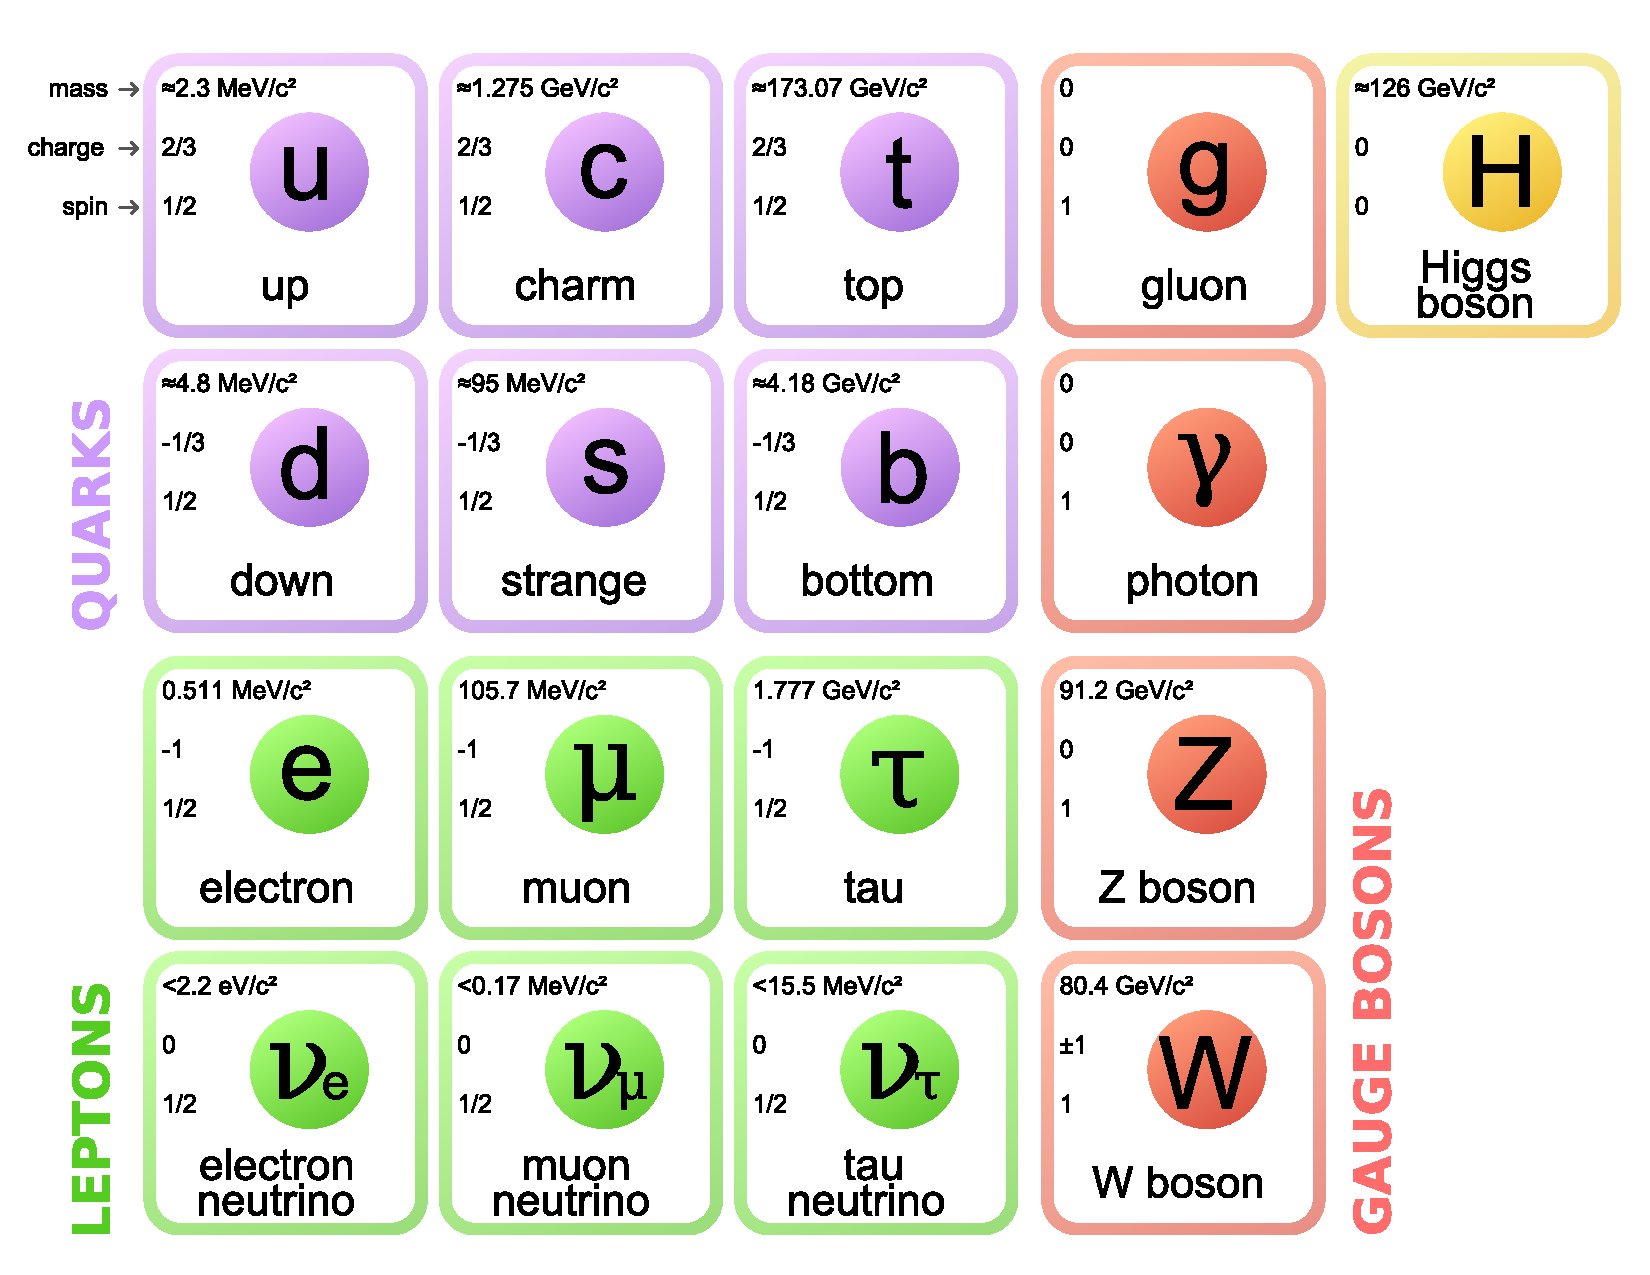
\includegraphics[width=0.8\textwidth]{particles.pdf}
\caption[The list of fundamental Standard Model particles broken down by particle type]
{\label{fig:intro_particles}
The list of fundamental Standard Model particles broken down by particle type:
quarks in purple, leptons in green, gauge bosons in red, and the Higgs boson in
yellow. The anti-quarks and anti-leptons are not shown~\cite{wikiparticles}.
}
\end{figure}
% --------------------------------------------------------------------------- %

% --------------------------------------------------------------------------- %
\subsubsection{Fermions}
\label{sec:intro_sm_fermions}
% --------------------------------------------------------------------------- %
The SM includes twelve spin-$\rm{\frac{1}{2}}$ elementary particles known as
fermions that make up all known matter in the universe. These fermions respect
the Pauli exclusion principle and each has a corresponding anti-particle. The
SM classifies the fermions according to how they interact through the quantum
numbers they carry. There are six quarks each assigned a different flavor
quantum number: up, down, charm, strange, top, and bottom. The remaining six
fermions are the leptons which are also identified by their flavor: electron,
electron neutrino, muon, muon neutrino, tau, and tau neutrino. Pairs from each
are classified and grouped together to form generations, which correspond to
particles exhibiting similar physical behavior.

The major property of the quarks is that they carry the color charge and
interact via the strong interaction. A phenomenon called color confinement
results in quarks being bound to one another, forming color neutral composite
particles called hadrons. Hadrons fall into two main categories: mesons which
are quark and antiquark bound states and baryons which are bound states of
three quarks (or three antiquarks). The familiar proton and the neutron are the
two baryons with the lowest mass. Quarks also carry electric and weak charges
and hence, they interact with all fermions via both the electromagnetic and
weak interactions.

The other main category of fermions, the leptons, do not carry color charge
and do not participate in the strong interaction. The three neutrinos do not
carry electric charge either, so they are only influenced by the weak nuclear
force. This property leads neutrinos to be notoriously difficult to detect
experimentally. However, the remaining three leptons do carry electric charge:
the electron, muon and tau all interact electromagnetically.

All 12 fermions are grouped into three generations where each member of
a generation has a greater mass than the corresponding particle in lower
generations. The first generation of quarks and leptons do not decay; hence
all ordinary matter is made up of such particles. Specifically, all atoms
consisting of electrons orbiting the nucleus which is made up of up and down
quarks. Second and third generations particles are very short lived and are
only produced in very high-energy environments (such as the LHC). Neutrinos
of all generations also do not decay and very rarely interact with matter.

% --------------------------------------------------------------------------- %
\subsubsection{Bosons}
\label{sec:intro_sm_bosons}
% --------------------------------------------------------------------------- %
In the SM, gauge bosons play the roll as the ``force carriers'' and are the
mediators of the strong, weak and electromagnetic fundamental forces or
interactions. The SM explains such forces as resulting from matter particles
exchanging these bosons, known as force mediators. At a macroscopic level, the
effect is equivalent to a force field influencing both of them; however, when
looking at the microscopic level, a gauge boson has been exchanged. The gauge
bosons of the SM all have spin-1, and as a result, they do not follow the Pauli
exclusion principle that constrains fermions and thus have no limit on their
spatial density. The different types of gauge bosons are described below:
% --------------------------------------------------------------------------- %
\begin{itemize}
\item Photons ($\gamma$) mediate the electromagnetic interaction between
charged particles. The photon is massless and is described by the subset of the
SM known as quantum electrodynamics.
\item The $W^+$, $W^-$, and Z gauge bosons mediate the weak interactions
between particles of different flavors (all quarks and leptons). They are
massive with the $W^{\pm}$ and Z bosons being 80.4 \GeVcc and 90.2 \GeVcc,
respectively~\cite{pdg}. The $W^+$ and $W^-$ bosons carry an electric charge
(indicated by the superscript) and the Z boson is electrically neutral. The
final characteristic is that the W bosons decay weakly into final states of
either two quarks or two leptons. In the case of the two quark final state, one
quark must be a up-type quark (up, charm) and the other a down type anti-quark
(down, strange, or bottom). The W does not decay via a top quark due to
kinematic constraints imposed by the much more massive top quark. In the case
where the W boson decays to a lepton pair, one lepton must be a charged lepton
(electron, muon, or tau) and the other must be a neutrino (electron neutrino,
muon neutrino, or tau neutrino). Finally, the Z boson must decay to a fermion
and its anti-particle. For example $\Zlplm$ or $Z \to q\bar{q}$ where $q$
represent a quark, $\bar{q}$ represents an antiquark, and $\ell$ represents a
charged lepton.
\item The eight gluons (g) mediate the strong interactions between color
charged particles (the quarks). Gluons are massless. The eightfold multiplicity
of gluons is labeled by a combination of color and anticolor charge, and
because gluons themselves carry a color charge, they can interact
among themselves. The gluons and their interactions are described by the theory
of chromodynamics.
\end{itemize}

% --------------------------------------------------------------------------- %
The final boson in the SM is the Higgs boson and is a key building block
in the underlying structure of the theory. It has no intrinsic spin
(scalar), is massive at 125.7 \GeVcc~\cite{higgstwiki}, and plays a unique roll by
explaining why other elementary particles, except the photon and gluon, are
massive~\cite{discovery}. In particular, they explain why the photon has no
mass, while the W and Z bosons do. Also, in electroweak theory, the Higgs
boson generates the masses of the leptons and quarks. Finally, as the Higgs is
massive, it must interact with itself.

The following Figure~\ref{fig:intro_int} shows a summary of all the allowed
interaction between particle types in the Standard Model.
% --------------------------------------------------------------------------- %
\begin{figure}[!hbt]
\centering
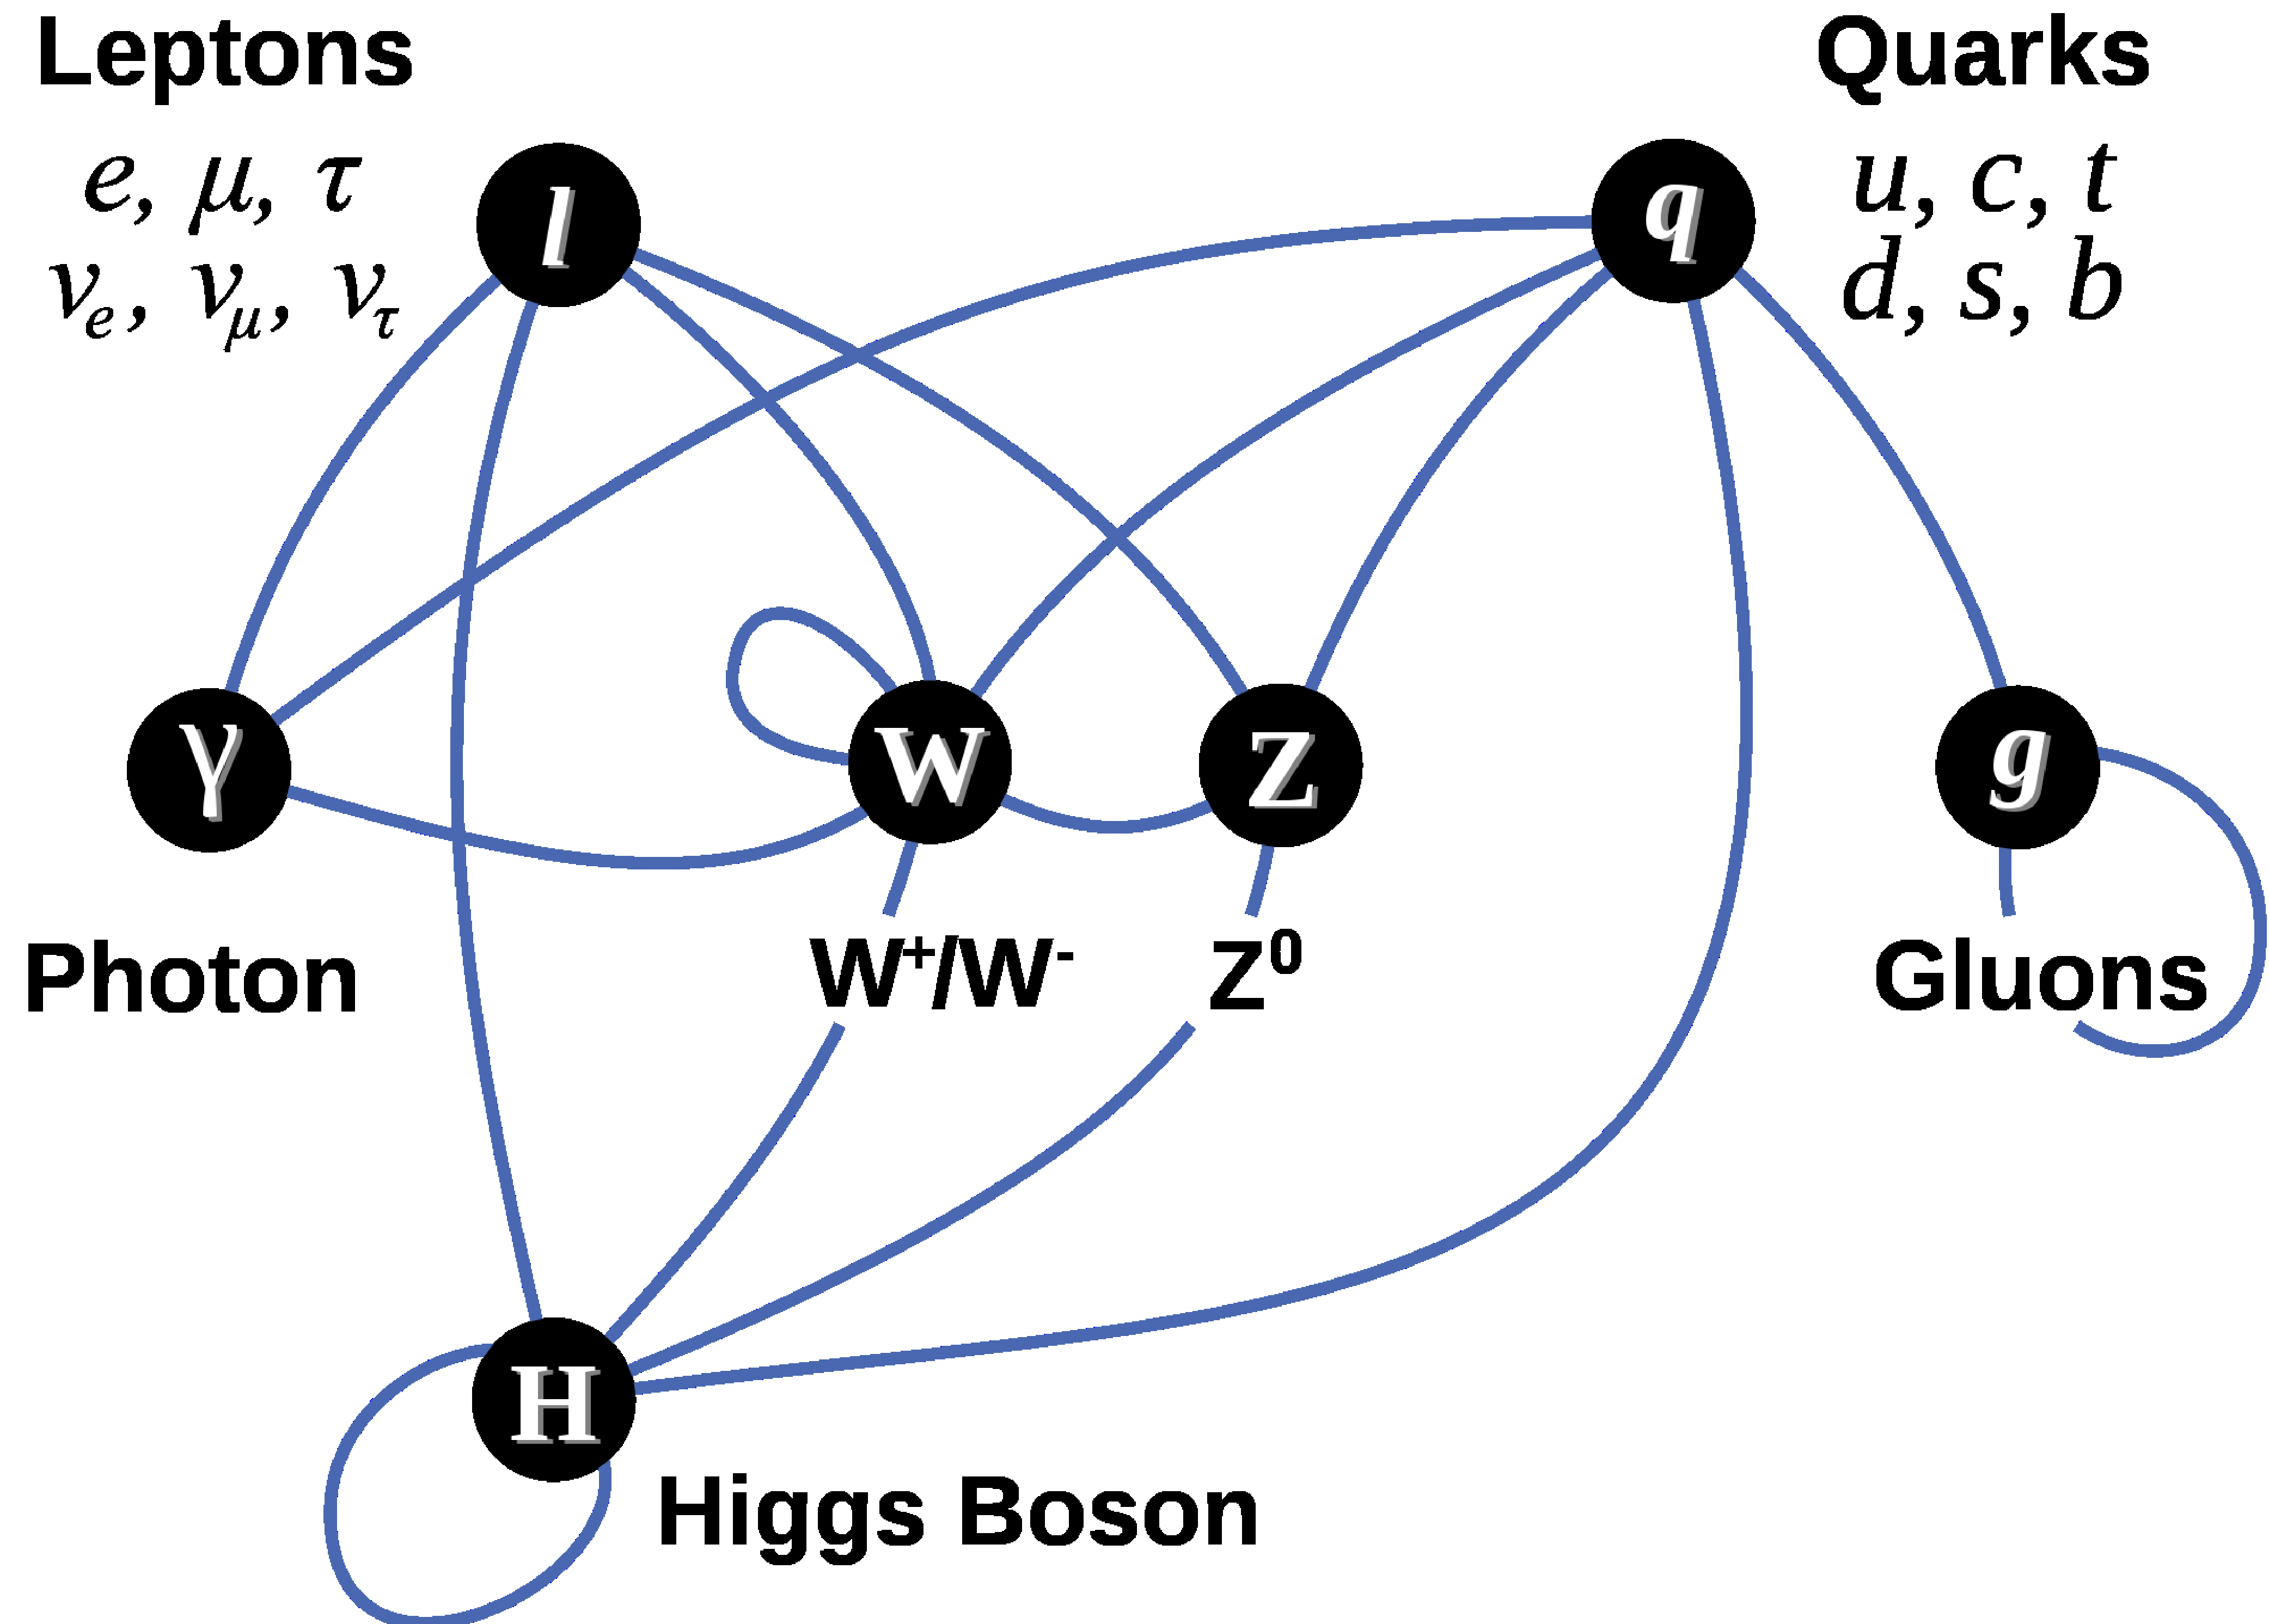
\includegraphics[width=0.6\textwidth]{interactions.pdf}
\caption[A summary of the allowed interactions between particle types in the Standard Model]
{\label{fig:intro_int}
A summary of the allowed interactions between particle types in the
Standard Model. A line connecting two particles indicates coupling occurs
between those particles. A line from one particle to itself indicates
that this particular particle self-couples~\cite{wikiinteractions}.
}
\end{figure}
% --------------------------------------------------------------------------- %

% --------------------------------------------------------------------------- %
\subsubsection{Known deficiencies of the SM}
\label{sec:intro_sm_issues}
% --------------------------------------------------------------------------- %
The Standard Model is not considered a complete theory. Some of the major
issues are outlined below:
% --------------------------------------------------------------------------- %
\begin{itemize}
\item The SM does not provide a mechanism to explain gravitation. Attempts have
been made to find a quantum theory of gravity that is also consistent with
general relativity; however, these theories break down before reaching the
Planck scale and therefore are not satisfactory.
\item The SM is considered {\it ad hoc} and inelegant since it requires many
numerical constants that seem arbitrary and unrelated.
\item The Higgs mechanism gives rise to the hierarchy problem if any new
symmetries or particle interactions are present at a high energy scale. In
order for the weak scale to be much smaller than the Planck scale, severe fine
tuning of the SM parameters is required.
\end{itemize}
% --------------------------------------------------------------------------- %
Also there are many questions in physics that are unanswered by the SM. Some of
these issues include:
% --------------------------------------------------------------------------- %
\begin{itemize}
\item Why do particle masses and coupling constants have the values that we measure?
\item Why are there three generations of particles?
\item Why is there more matter than antimatter observed in the universe?
\item Where does dark matter fit into the model?
\item Where does dark energy fit into the model?
\end{itemize}
% --------------------------------------------------------------------------- %
Clearly the SM does not provide the final explanation of all the observed
interactions in nature.

% --------------------------------------------------------------------------- %
% --------------------------------------------------------------------------- %
\section{Proton-Proton Collisions}
\label {sec:intro_collider}
% --------------------------------------------------------------------------- %
% --------------------------------------------------------------------------- %
To probe some of the unanswered question from the SM posed in the previous
Section (Section~\ref{sec:intro_sm}), protons are collided at high energy and
their debris is studied in detail. In particle physics, the probability for an
interaction to occur is given by the cross section ($\sigma$), which represents
the effective area presented by the target to an incoming particle. The units
for cross section are given in terms of a barn (b) where $1\ \barn = 10^{-24}\
\rm{\cm^2}$. The total number of interactions is given by the relation
% --------------------------------------------------------------------------- %
\begin{equation}
    N = \Lumi \cdot \sigma,
\end{equation}
% --------------------------------------------------------------------------- %
where $N$ is the number of interactions occurring in an instantaneous
luminosity of \lumi for a process with an interaction cross section $\sigma$.
The total amount of data collected is traditionally reported as the total
integrated luminosity reported by the above relation. The integrated luminosity
has units of inverse barns (\binv); however, due to the inconvenience of the
scale of this unit, it is customary to report the units in either inverse
picobarns (\pbinv = $10^{12}$ \binv) or inverse femtobarns (\fbinv = $10^{15}$
\binv).

The difficulty of producing and storing antiprotons led to the decision to use
proton-proton (pp) collisions at the LHC~\cite{lhcmachine}. The cross section
for a typical pp collision $\approx 100$ mb~\cite{qcdprimer}. This however,
combines both elastic collisions, where the two colliding protons remain whole,
and inelastic collisions, where the proton breaks apart into its constituent
quarks or gluons (partons). For inelastic collisions, QCD does not allow for
a quantitative calculation of the exact kinematics of the partons that make
up the proton. Instead, one has to appeal to a series of experiments designed
to create an empirical model of the kinematic distributions of these partons.
This is done with deep inelastic scattering experiments where a high energy
electron is collided with the proton~\cite{halzen}. By measuring the resulting
momentum and angular distributions of the proton's debris, one can determine of
the fraction of energy carried by the partons which make up the proton. As an
example, Figure \ref{fig:intro_partons} shows the fraction of energy carried by
gluons and quarks for two different energy protons. Notice that while the up
and down quarks and the gluons are the dominant high momentum carriers, there
is still significant momentum from the other partons (sea quarks).

% --------------------------------------------------------------------------- %
\begin{figure}[tbhp]
\centering
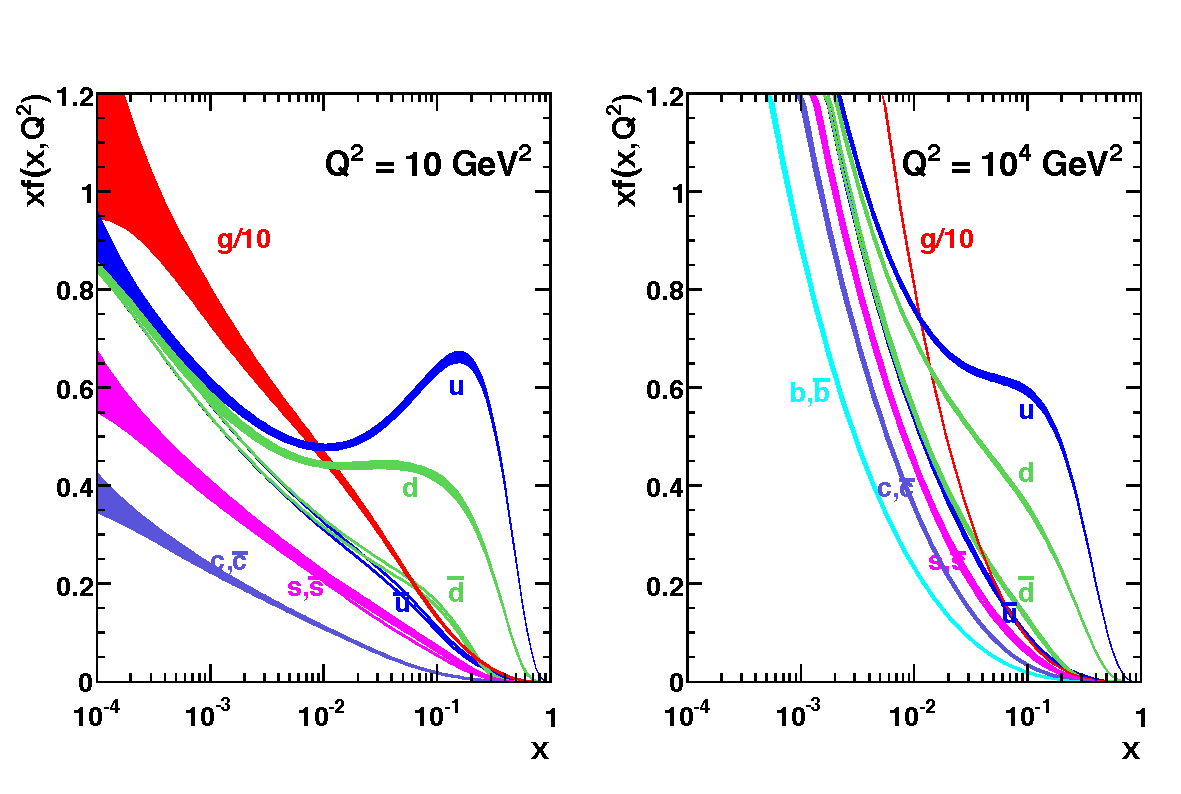
\includegraphics[width=0.8\textwidth]{partons}
\caption[Parton distribution functions for protons at $Q^2=10~\GeV^2$ and $Q^2=10000~\GeV^2$] 
{\label{fig:intro_partons}
The parton distribution functions and their associated error
for a proton at a momentum transfer scale of $Q^2=10~\GeV^2$ (left) and
$Q^2=10000~\GeV^2$ (right) as a function of $x$, the fraction of the proton's
momentum carried by the parton~\cite{partons}.
}
\end{figure}
% --------------------------------------------------------------------------- %

% --------------------------------------------------------------------------- %
% --------------------------------------------------------------------------- %
\section{Motivation for Same-Sign Dilepton Signature}
\label {sec:intro_ss}
% --------------------------------------------------------------------------- %
% --------------------------------------------------------------------------- %
One of the purposes of the LHC and CMS is to search for physics beyond
the Standard Model (BSM). As mentioned in Section~\ref{sec:intro_sm},
astrophysical evidence for dark matter suggests that the SM is incomplete.
Although direct detection experiments have yet to make an observation,
indirect measurements are pointing to dark matter being related to the weak
interaction~\cite{darkmatter,baer}. It is clear that the SM is not the full
story describing particle interactions. The physics analysis discussed in this
thesis attempts to take advantage of the strengths in lepton reconstruction
to search for previously unobserved physics.

Figure~\ref{fig:intro_smxsec} shows the production cross section for a number of SM
processes as a function of the center-of-mass energy of the colliding beams.
% --------------------------------------------------------------------------- %
\begin{figure}[tbhp]
\centering
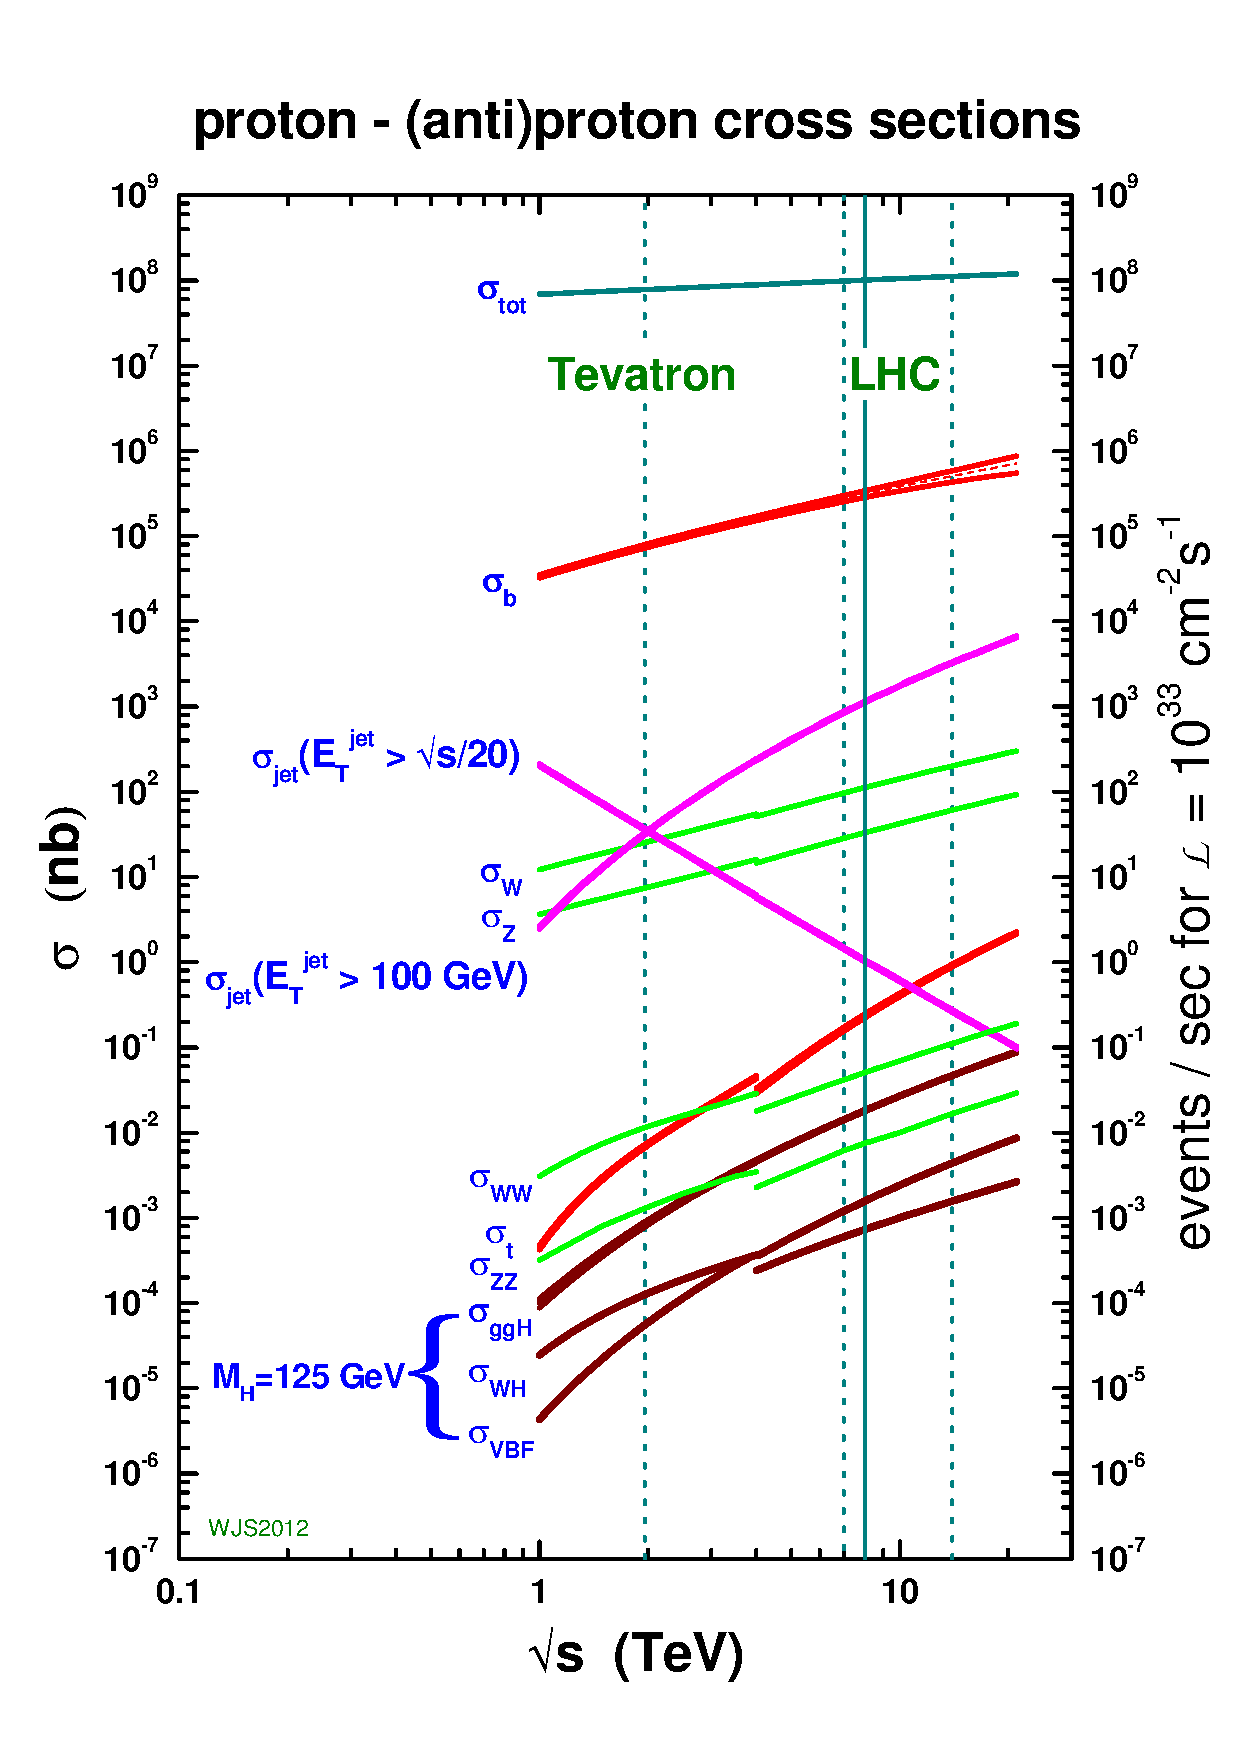
\includegraphics[width=0.8\textwidth]{smxsec}
\caption[Cross sections for some Standard Model process vs center-of-mass energy] 
{\label{fig:intro_smxsec}
Cross sections for some Standard Model processes vs center-of-mass energy.
The cross sections of SM process giving final state leptons are many orders of
magnitude smaller than QCD cross sections. From~\cite{smxsec}.
}
\end{figure}
% --------------------------------------------------------------------------- %
Comparing the relative size of the total inelastic collisions cross section,
contaminated by QCD processes, with that for W boson production, it is apparent
that these electroweak processes are rare in the SM. Subsequent leptonic
decays of the W boson occurs at the rate of $\approx 30\%$, making leptons
originating from a W boson even more rare. Sources of dilepton final states
are significantly more rare with the dominant source being \Zlplm. Additional
sources of dileptons include \ttbar, \WW, \WZ, and \ZZ production, all
with smaller production cross sections. Most of the dilepton pairs from these
have opposite electric charge (+/-). Since these lepton are both prompt and
relatively isolated, they provide an extremely clean experimental signature
in the detector since they are simpler to reconstruct with smaller rates of
mis-measurement. The combined effect is much smaller backgrounds for searches
in dilepton final states, particularly same-sign dilepton final states ({+}{+}
or {-}{-}), compared to single lepton and fully hadronic analyses.

From the above discussion, it is clear that a signature with two prompt and
isolated leptons with the same electric charge (same-signed dileptons) is a
rare occurrence in the SM relative to other processes. As a result, searches
for anomalous production of same-sign dileptons can be very sensitive to new
physics contributions. These include
% --------------------------------------------------------------------------- %
\begin{itemize}
\item supersymmetry (SUSY) \cite{ss::barnett,ss:baer,ss:guchait},
\item universal extra dimensions \cite{ss:cheng}
\item pair production of $T_{5/3}$ particles (fermionic parters of the top quark) \cite{ss:contino}, 
\item heavy Majorana neutrinos \cite{ss:almeida},
\item and same-sign top pair production \cite{ss::sstop}.
\end{itemize}
% --------------------------------------------------------------------------- %
New physics signatures with large cross sections are likely to be produced
by strong interactions, and we thus expect significant hadronic activity in
conjunction with the two leptons. Additionally, SUSY models with R-parity
conservation and astrophysical evidence for dark matter suggest considering
final states with undetectable particles that leads to a significant amount
of missing transverse energy (\met)~\cite{AMS,Bertone:2004pz}. With the above
considerations, in this analysis, we search for new physics with events
containing:
% --------------------------------------------------------------------------- %
\begin{itemize}
\item same-sign dileptons (electrons and muons), 
\item hadronic jets (with and without b-tagging), 
\item and accompanying missing transverse energy.
\end{itemize}
% --------------------------------------------------------------------------- %
The exact event selection will be discussed in Chapter~\ref{ch:evtsel}.

The basic idea is to count the number of observed collision events that have
the above signature and compare this to the number of events that were expected
assuming the SM only. This comparison is done using statistical techniques
to be discussed in Section \ref{sec:results_int}. If there is a significant
excess of events above your expected SM background, then this gives evidence
that new physics exists beyond the SM. It is important to get the most accurate
background prediction possible to ensure maximum sensitivity to an anomalous
excess of events. The specific details of the background estimation techniques
can be found in the following chapters. Finally, in Chapter \ref{ch:results},
we show the results of this search along with some interpretations with respect
to some selected new physics models.

% --------------------------------------------------------------------------- %
% --------------------------------------------------------------------------- %
\chapter{The LHC Accelerator and CMS Experiment}
\label {ch:cms}

The Compact Muon Solenoid (CMS) experiment is a collaboration of scientists
working together to investigate the data streaming from the Large Hadron
Collider (LHC). This chapter will give an overview of the experimental setup
used by the nearly 3,000 CMS collaborators to analyze this data. First 
we give a short discussion of the Large Hadron Collider followed by
the Compact Muon Solenoid detector itself. Finally, we will give a brief
description of the algorithms used to measure the particles traversing the CMS
detector used by the various analyses.

% --------------------------------------------------------------------------- %
% --------------------------------------------------------------------------- %
\section{The Large Hadron Collider}
\label {sec:cms_lhc}
% --------------------------------------------------------------------------- %
% --------------------------------------------------------------------------- %

As previously discussed in Chapter~\ref{ch:intro}, the Standard Model of
particle physics (SM) is the de facto theory that currently describes all
known particle interactions save gravity. The aim of the Large Hadron Collider
(LHC) is to invesitage the possibility of physics beyond the Standard Model.
Completed in 2008, it is approximately 27 km in circumference, sits 170
meters underground and was designed to accelerate protons to 7 \TeV~each and
collide them at four interaction points. Each interaction point has a detector
positioned there to record the outcome of these proton-proton collisions: the
two general purpose detectors CMS and ATLAS, and the other two specialized
detectors ALICE and LHC-b. Figure \ref{fig:cms_underground}~shows a cartoon of
the LHC and the four particle detectors which is located on the outskirts of
Geneva, Switzerland.

% --------------------------------------------------------------------------- %
\begin{figure}[tbhp]
\centering
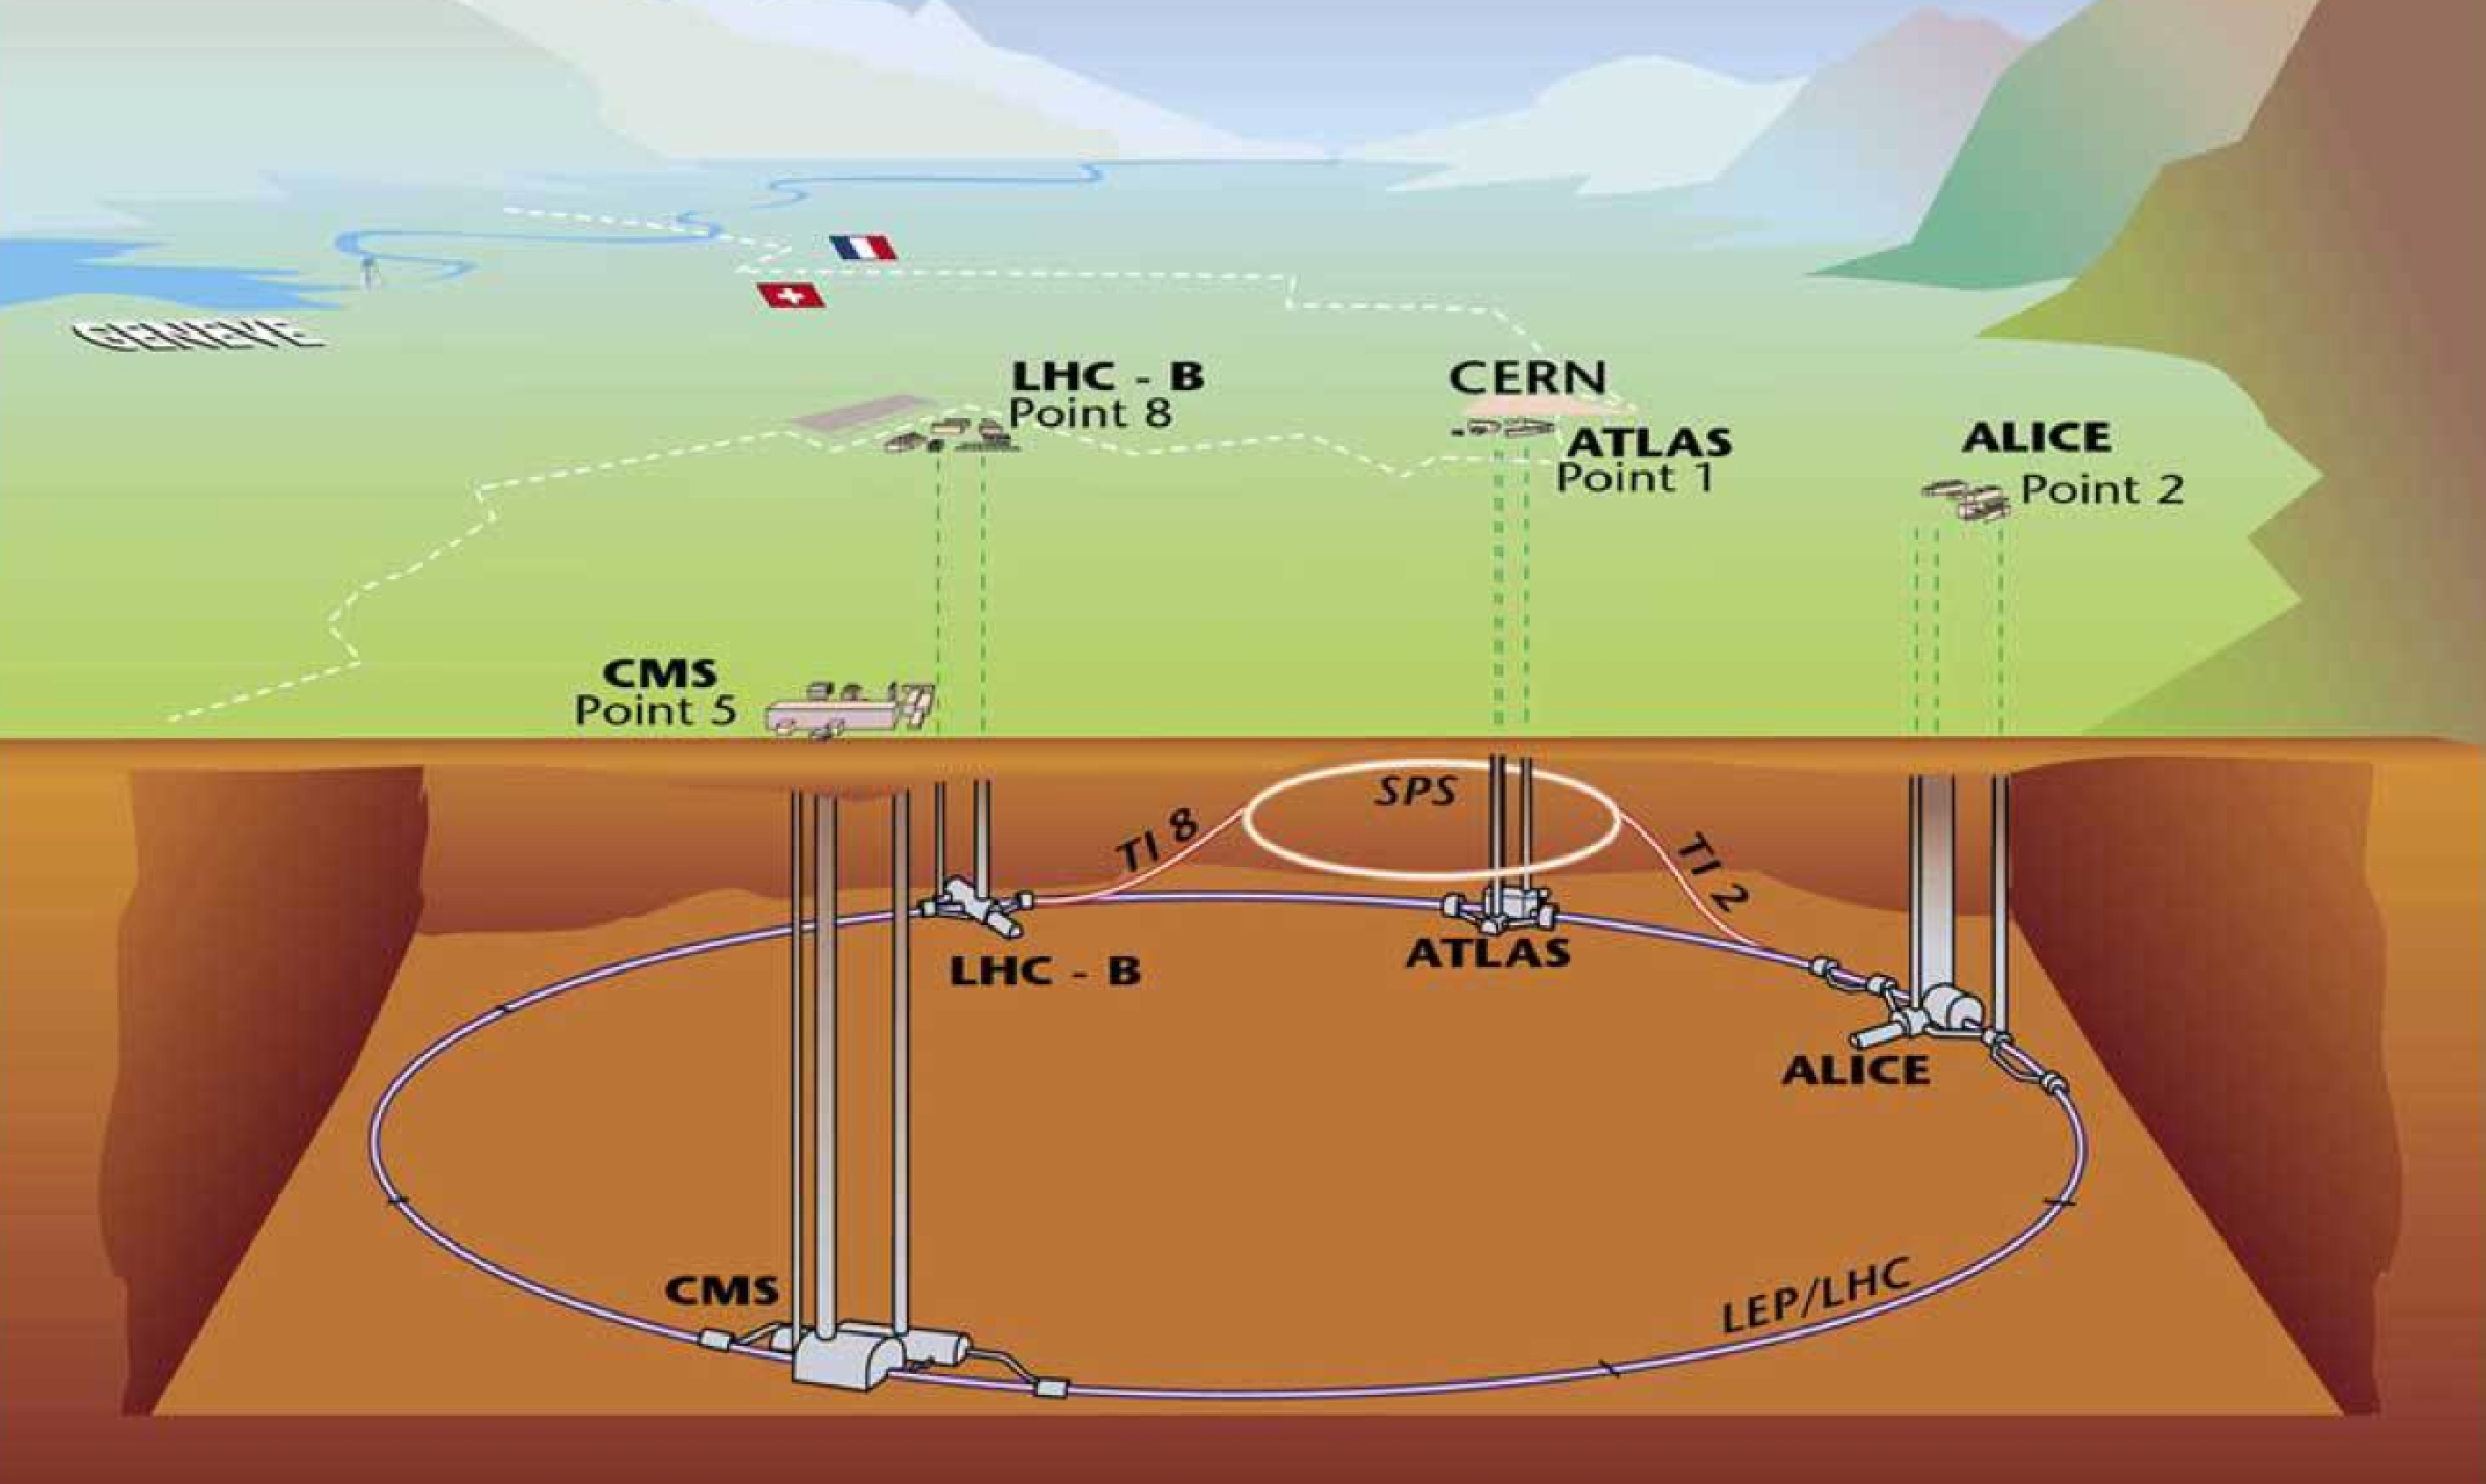
\includegraphics[width=0.9\textwidth]{underground.pdf}
\caption[The Large Hadron complex seen underground on the outskirts of  Geneva, Switzerland]
{\label{fig:cms_underground}
The Large Hadron complex seen underground on the
outskirts of Geneva, Switzerland. The four detectors main detectors are also shown -- LHC-B, ATLAS, ALICE, and, most
relevant to this analysis, CMS at Point 5~\cite{lhcmachine}.
}
\end{figure}
% --------------------------------------------------------------------------- %

The search for the Higgs boson carried a large influence on the design of
the Large Hadron Collider (LHC) and the CMS detector. The previously unknown
mass of the Higgs boson combined with its small production cross section
required building a machine capable of high energy collisions at a high rate.
This design leads to approximately 1 billion proton-proton collisions per
second~\cite{lhcmachine}. Rather than continuous beams, the protons will be
``bunched'' together, into 2,808 bunches, 115 billion protons in each bunch so
that interactions between the two beams will take place at discrete intervals
never shorter than 25 nanoseconds (ns) apart. The design luminosity of the LHC
is $10^{34} \rm{cm^{−2}s^{−1}}$, providing a bunch collision rate of 40 MHz.

Although the design center-of-mass energy ($\sqrt{s}$) is 14 TeV, the data 
collected from 2011 and 2012 was at $\sqrt{s} = 7\ \TeV$ and $8\ \TeV$, respectively.
The data used for this thesis is the full dataset recorded from 2012 at 
$\sqrt{s} = 8\ \TeV$. The LHC plans to continue collisions in 2015 at $\sqrt{s}
= 13\ \TeV$.

% --------------------------------------------------------------------------- %
% --------------------------------------------------------------------------- %
\section{The Compact Muon Solenoid Detector}
\label {sec:cms_cms}
% --------------------------------------------------------------------------- %
% --------------------------------------------------------------------------- %
The Compact Muon Solenoid (CMS) is one of the two general purpose detectors
situated along the beam line of the LHC. The name ``compact'' comes from
the fact that the detector is relatively small when compared to it's
sister experiment known as A Toroidal LHC Apparatus (ATLAS); however, CMS
is by no means small. Weighing in at over 12,000 tons, cylindrical in
shape, it is over 21 meters in length and 14 meters in diameter. It sits
$\sim$100 meters underground at LHC Point 5 near Cessy, France (see Figure
\ref{fig:cms_underground}). An overview of the CMS detector can be seen in
Figure \ref{fig:cms_diag}.
% --------------------------------------------------------------------------- %
\begin{figure}[tbhp]
\centering
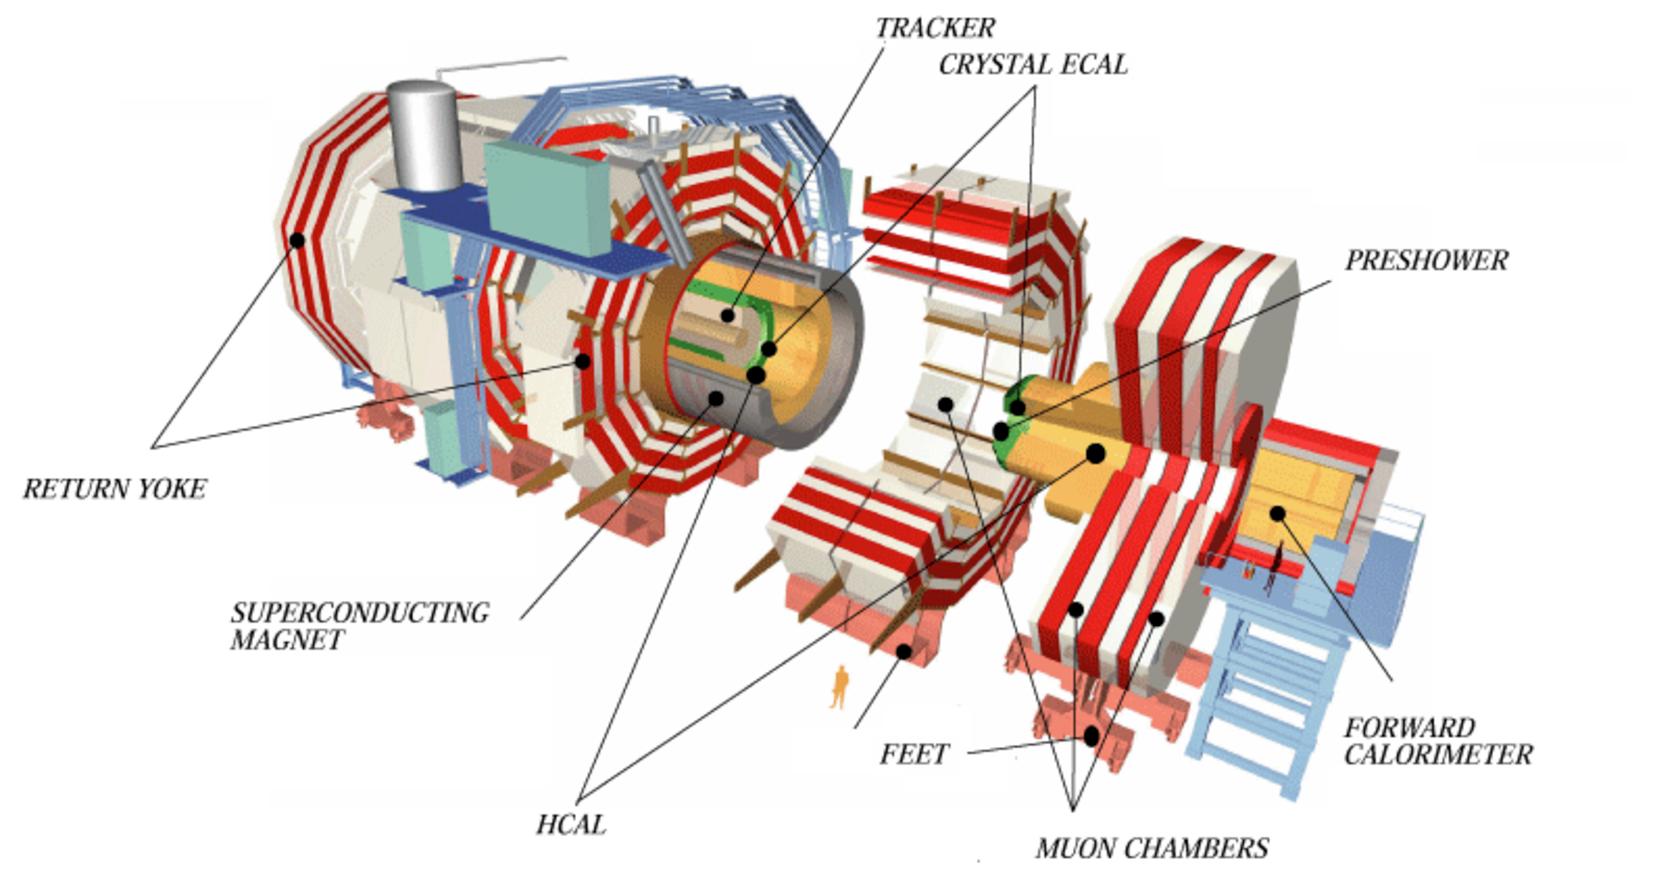
\includegraphics[width=0.9\textwidth]{cms_diag.pdf}
\caption[Overview of the Compact Muon Solenoid detector]
{\label{fig:cms_diag}
Overview of the Compact Muon Solenoid detector~\cite{cmspic}.
}
\end{figure}
% --------------------------------------------------------------------------- %
CMS was designed to allow for the study of many different unanswered questions
in particle physics. To achieve this broad objective, CMS is capable of
measuring with high precision, the trajectory, momentum and energy of many
different types of particles. In addition, it is able to handle the challenging
conditions presented by the high luminosity and high energy collisions from
the LHC. To deal with the approximately one billion interactions per second
expected from the LHC at its design luminosity, CMS is a very high granular
detector, and hence has many electronic channels, each with excellent time
resolution and is designed to be radiation hard to deal with the multitude of
particles produced during each bunch crossing.

CMS contains a strong magnetic field produced by a superconducting solenoid.
An inner field strength of 3.8 Tesla ensures that even the highest momentum
particles propagating through the detector have enough curvature to ensure a
precise momentum measurement. Inside the solenoid sit both the silicon and
pixel tracker systems and both the electromagnetic (ECAL) and hadronic
calorimeters (HCAL). The larger number of channels in the pixel tracker
ensure a precise measurement of the origin of particles both produced near
the beamline and those with longer lifetimes decaying at larger diameters.
The silicon strip detector has at least 10 layers along any particles' path
allowing precise particle ``tracking'' and momentum measurements. The ECAL,
with over 75,000 lead-tungstate (\pbw) scintillating crystals, gives
excellent energy measurements of the particles which interact primarily
electromagnetically, namely electrons and photons. The HCAL, a sampling
calorimeter made of brass, completes the sub-detectors existing inside of the
solenoid and gives respectable energy resolution for particles that interact
primarily hadronically (e.g. pions and kaons).

Outside of the solenoid rests the final major sub-detector, the muon detector.
Made up of three separate components, the muon chambers are placed between the large
iron frame (yoke) that serves two purposes. First, they prevent particles
other than muons from reaching the outermost muon chambers and hence allow for
excellent muon identification. Secondly, the yoke allows for a strong return
magnetic field to fill the entirety of the muon detector system which allows
for better momentum resolution.

The coordinate system of CMS is centered at the nominal interaction point at
the center of CMS's cylindrical shape. We define the y-axis to point upwards
(away from the center of the earth), the x-axis the points towards the center
of the LHC ring and hence, the z-axis points along the beamline, counter
clockwise around the LHC. The azimuthal angle, $\phi$, is measured from the
zero position of the x-axis in the x-y plane while the polar angle, $\theta$, is
measured from the positive z-axis.

Finally, we should introduce now two important quantities used in hadronic
collider physics. While we know precisely the center-of-momentum frame
and individual momenta of the two colliding protons, we do not know the
center-of-momentum frame for the two colliding partons. For this reason, we
define two quantities that are invariant under a boost in the direction of the
proton's momentum. The first quantity is the partons' momentum in the plane
normal to the collision -- i.e. the transverse plane, the transverse momentum
(\pt) can be defined and is, to first order, conserved. The second quantity,
pseudorapidity ($\eta$) is a transformation from the polar angle into an
invariant quantity with respect to the frame of the collision:

% ---------------------------------------------------------------------------
\begin{equation}
    \eta = - \rm{ln} \left[\rm{tan}\left(\frac{\theta}{2}\right)\right],
\end{equation}
% ---------------------------------------------------------------------------
where $\theta$ is the angle between the incoming proton and the outgoing
particle. These two quantities, \pt and $\eta$, are used extensively at the
LHC to describe the kinematics of the out going particles from a proton-proton
collision and will be used throughout this analysis as well.

A complete description of the CMS detector can be found in Reference~\cite{jinst},
from which all information in this section is derived, unless explicitly
stated. The following subsections give a more detailed description of the various
pieces that make up the CMS detector. This is not meant to be a full detector
description; however, we do highlight details that are important to the
analysis in this thesis.

% --------------------------------------------------------------------------- %
% --------------------------------------------------------------------------- %
\subsection{The Superconducting Solenoid}
\label {sec:cms_solenoid}
% --------------------------------------------------------------------------- %
% --------------------------------------------------------------------------- %
Charged particles in an electromagnetic field experience a force given by
\[
\mathbf{F} = q\left(\mathbf{E} + \mathbf{v}\times\mathbf{B}\right),
\]
where q is the charge of the paricle, $\mathbf{E}$ is the electric field,
$\mathbf{v}$ is the velocity of the charged particle and $\mathbf{B}$ is
the magnetic field. Therefore, for a uniform magnetic field, the radius of
curvature, r, of a charge particles is directly proportional to the particle's
momentum and inversely proportional to the magnetic field strength,
\[
r = \frac{\pt}{q |\mathbf{B}|},
\]
where \pt is the particles transverse momentum with respect to the direction
of the magnetic field. With $\sim$3 meters from the nominal interaction point
to the inside edge of the solenoid, CMS must have a strong magnetic field to
achieve the maximum possible curvature for the charged particles. This ensures
the most precise measurement of the momentum and this is achieved with CMS's
superconducting solenoid.

Made up of Niobium-Titanium ($\rm NbTi$), the solenoid was designed to operate
with a magnetic field strength of 4 Tesla, yet due to safety considerations,
is operated at 3.8 Tesla. At maximum strength, the solenoid stores over 2
Gigajoules of energy and far exceeds the design strength of all other particle
detectors.

To allow for this stronger magnetic field, and hence better momentum
measurement, for the muon chambers, the outside of the solenoid has been
designed with iron yokes which offer integral support, provide additional
stopping power for non-muons and propagates the magnetic field. The yokes can
be seen in red in Figure~\ref{fig:cms_diag}.

% --------------------------------------------------------------------------- %
% --------------------------------------------------------------------------- %
\subsection{The Silicon Detector}
\label {sec:cms_silicon}
% --------------------------------------------------------------------------- %
% --------------------------------------------------------------------------- %
The innermost portion of the CMS detector is comprised of a silicon based
particle tracking system (tracker). Doped and negatively biased, when charged
particles traverse the active region of the silicon, electric current is
induced and measured. This gives a positional measurement of the charged
particles and is recorded for later reconstruction (hits). Combining the
multiple positional measurements, the curvature of a charged particle is
measured, and thus, using the known magnetic field strength, the particle's
momentum. The tracker was designed to have a high efficiency to properly
reconstruct the trajectory, good momentum resolution and be able to identify
secondary vertices from longer lived particles such as b-flavored hadrons.

Many aspects of the tracker were specifically tailored to achieve the design
considerations discussed above and to physically fit within the CMS solenoid.
First, in order to deal with large particle multiplicities, the detector needed
to be radiation hard, have a high granularity and a fast electronic response
time. The high granularity was achieved by using a pixel silicon detector in the
inner most region. Outside of the pixel detector, silicon strips are used as
the particle multiplicity density decreases as the square of the radius from
the interaction point. This design achieves the desired position, momentum
and vertex resolution while keeping the occupancy down to a manageable 1\%
throughout. An overview of the layout of the silicon tracker can be see in
Figure~\ref{fig:cms_tracker} with the following subsections discussing the
pixel and strip detectors, respectively.
% --------------------------------------------------------------------------- %
\begin{figure}[tbhp]
\begin{center}
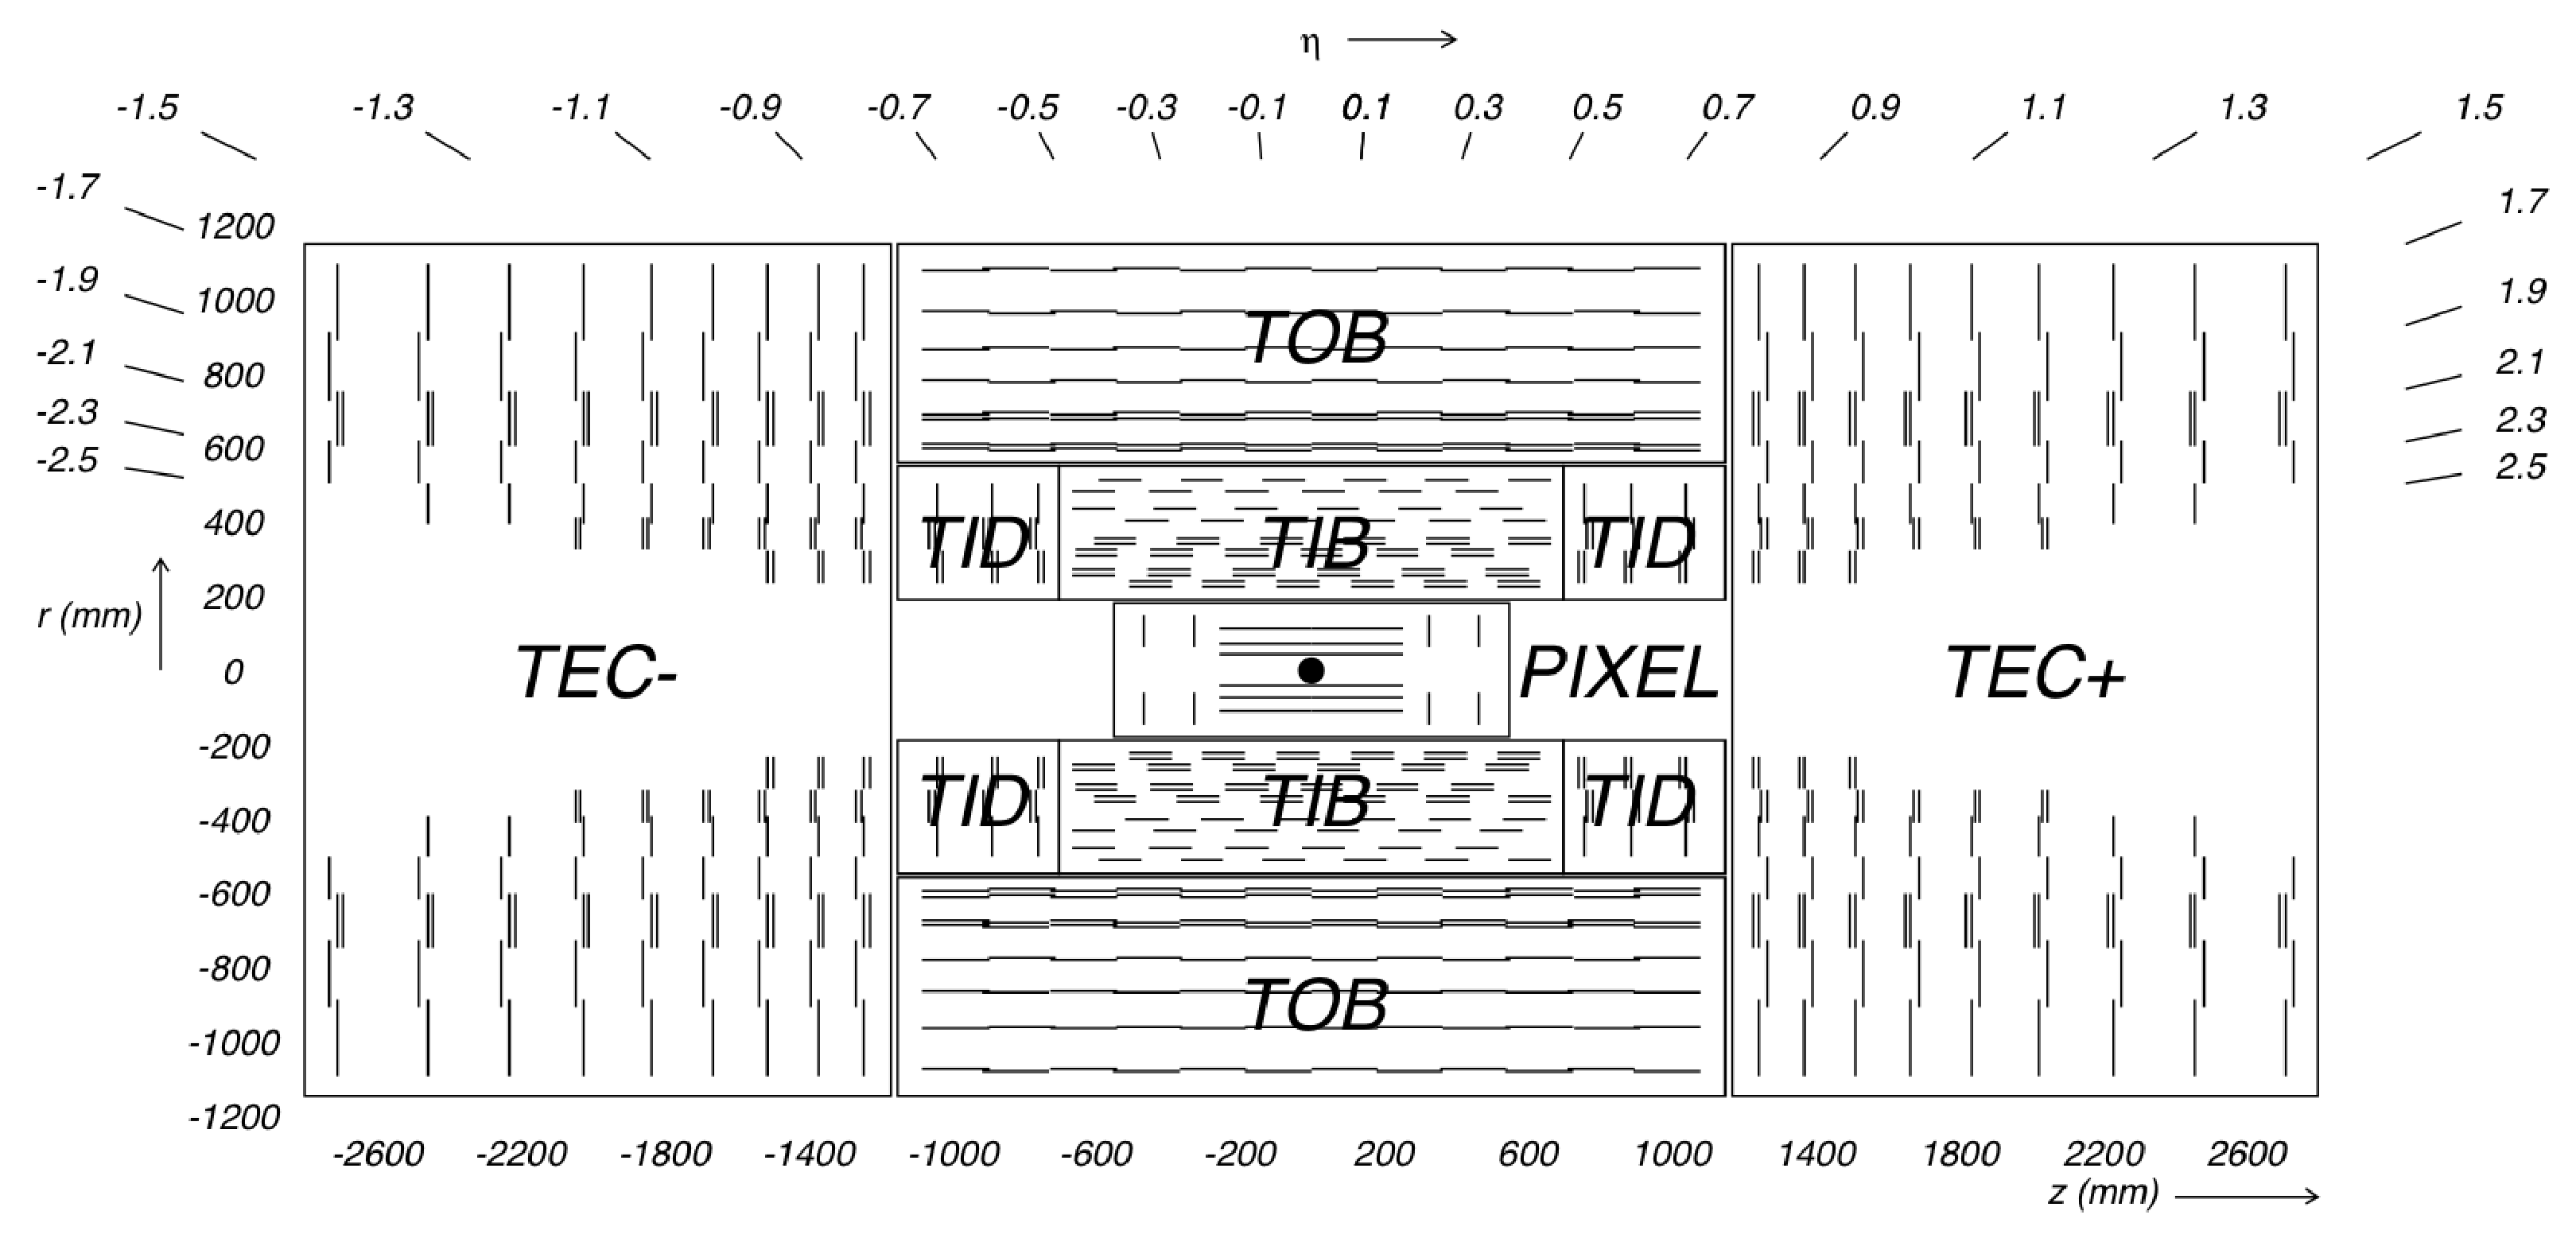
\includegraphics[width=0.95\textwidth]{tklayout.pdf}
\caption[Layout of the tracking system projected into the $rz$ plane]
{\label{fig:cms_tracker}
Layout of the tracking system projected into the $rz$ plane. Modules are
shown as lines and modules with back-to-back labels appear as double parallel
lines~\cite{trackingperformance}.
}
\end{center}
\end{figure}
% --------------------------------------------------------------------------- %

\subsubsection{The Pixel Detector}
\label {sec:cms_silicon_pixel}

In order to achieve the 1\% occupancy nearest the beam line, pixel silicon
detectors are used within a radius of $\sim$10 \cm. The CMS pixel detector
consists of three concentric cylindrical layers at 4.4, 7.4 and 10.2 \cm in
the radial direction with two disks at 34.5 and 45.6 \cm on each side along
the z-coordinate. Together, the ``barrel'' and ``endcap'' pixel detectors
cover a pseudorapidity range up to $\aeta < 2.5$. The pixels themselves
are approximately square with a size of 100 to 150 \um per side and have a
spatial resolution of 10 \um in the $r - \phi$ direction and 200 \um in the
z direction. Besides allowing for low occupancy, the pixel detectors are
also be made radiation hard and are designed to give precise vertex position
measurements.

\subsubsection{The Strip Detector}
\label {sec:cms_silicon_strip}

Outside of the pixel detector sits the silicon strip detector. At these
distances from the interaction point, a lower density of sensors can be
used to obtain the same occupancy. Strip detectors (long rectangular
active regions) are significantly cheaper to manufacture than pixel detectors
while still providing the desired momentum resolution and channel occupancy.
The strip detector can be divided into four different regions: the tracker
inner barrel (TIB), the tracker inner disks (TID), the tracker outer
barrel (TOB) and the tracker endcaps (TEC). Each region can be seen in
Figure~\ref{fig:cms_tracker}. The TIB consists of four cylindrical layers
in the barrel and is surrounded on each side by three disks from the TID. The
TIB and TID extend out to a radius of approximately 55 \cm and provide
position measurement resolution of between 23 and 35 \um. The TOB surrounds the
TIB and TID and provides another 6 cylindrical layers and provides slightly
less resolution of around 35 to 53 \um. Finally, the TEC extends out into the
z-direction by providing an additional 9 disk layers with resolution between 97
and 184 \um. The silicon strip detector also provides a pseudorapidity coverage
inside $\aeta < 2.5$. Some of the layers in the strip detector, namely the first
two layers in each TIB, TID, TOB and TEC as well as layer five in the TEC,
carry an additional offset detector mounted at a slight angle. This allows not
just for additional positional measurement but an additional measurement in the
``non-strip'' direction (z in the barrel and r in the endcaps).

\subsubsection{The Tracker}
\label {sec:cms_silicon_tracker}

With over 200 square meters of silicon, the CMS Tracker is the largest silicon
detector in the world. Unfortunately, material comes at a performance cost.
The silicon must all the powered, and in turn, the powered units must all
be cooled (operating temperate is $-10\ ^{\circ}\mathrm{C}$). The amount
of material in the CMS tracker is shown in units of radiation length in
Figure~\ref{fig:cms_material}. A radiation length is a characteristic of a
material and describes the distance over which electrons and photons lose
energy and is the length at which an electron, on average, will lose all but
$1/e$ of its initial energy via bremsstrahlung. All of this material inside CMS
causes a few complications. First, particle momentum resolution is degraded as
each particle has a higher probability for nuclear interaction and multiple
scattering as it traverses the detector. Second, electrons and photons have higher
probabilities to bremsstrahlung and pair create, respectively, causing issues
measuring their energy in the electromagnetic calorimeter (see next section).
% --------------------------------------------------------------------------- %
\begin{figure}[!htb]
\begin{center}
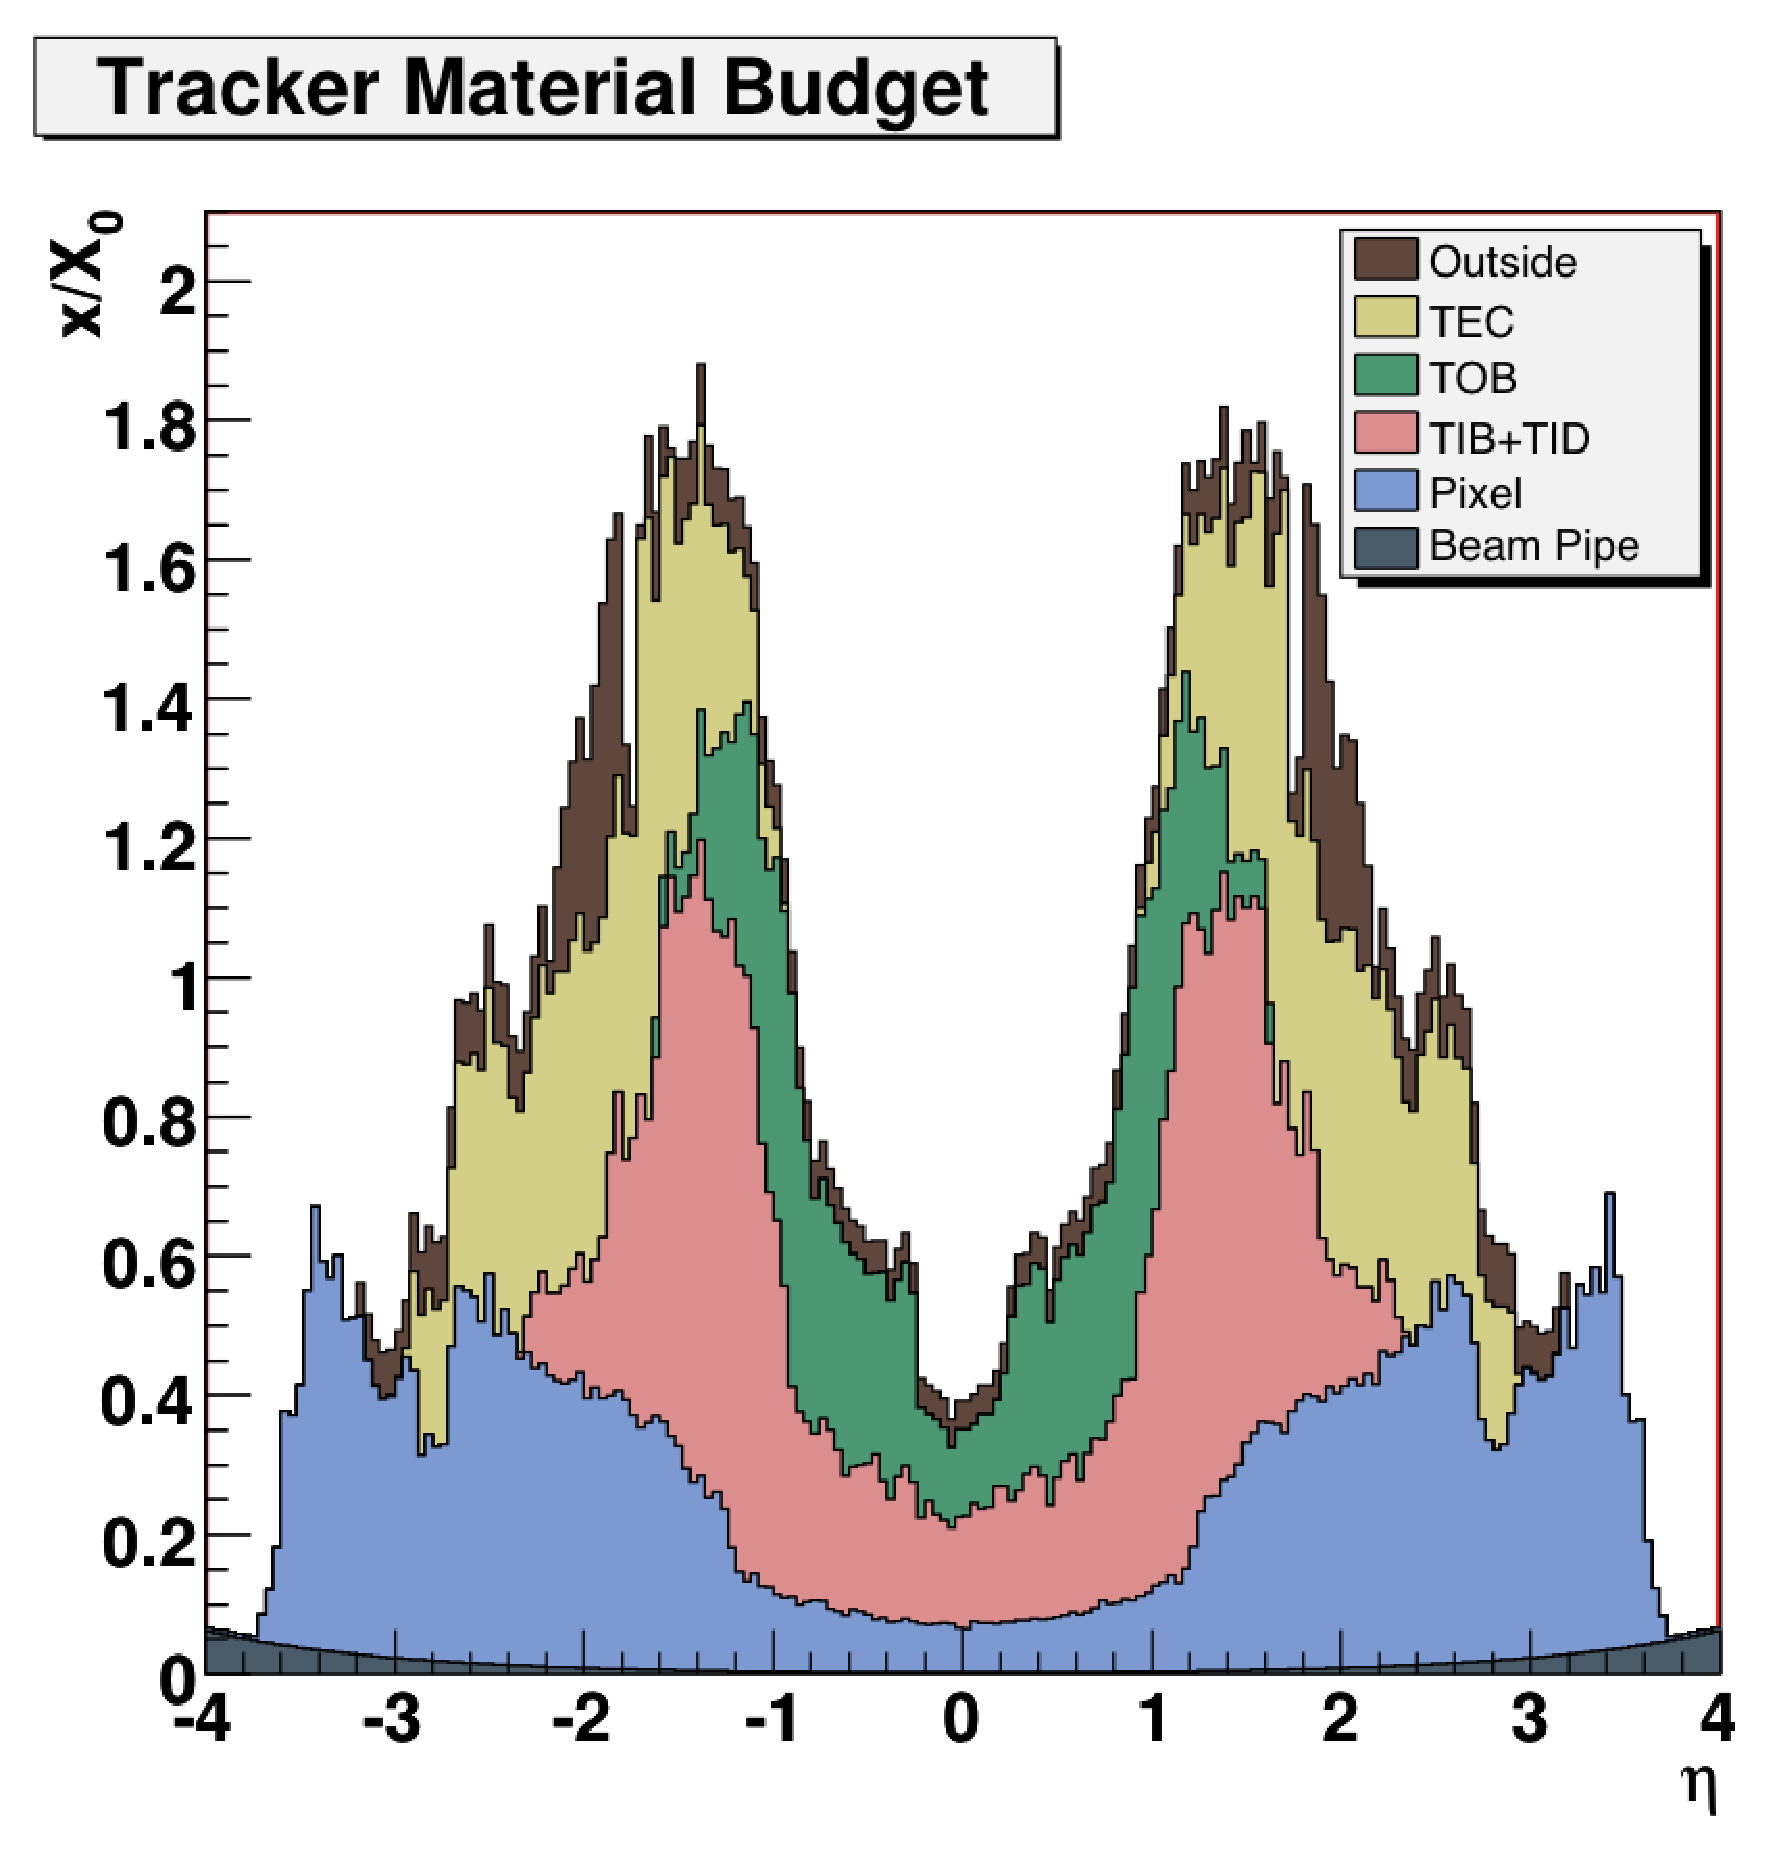
\includegraphics[width=0.4\textwidth]{material.pdf}
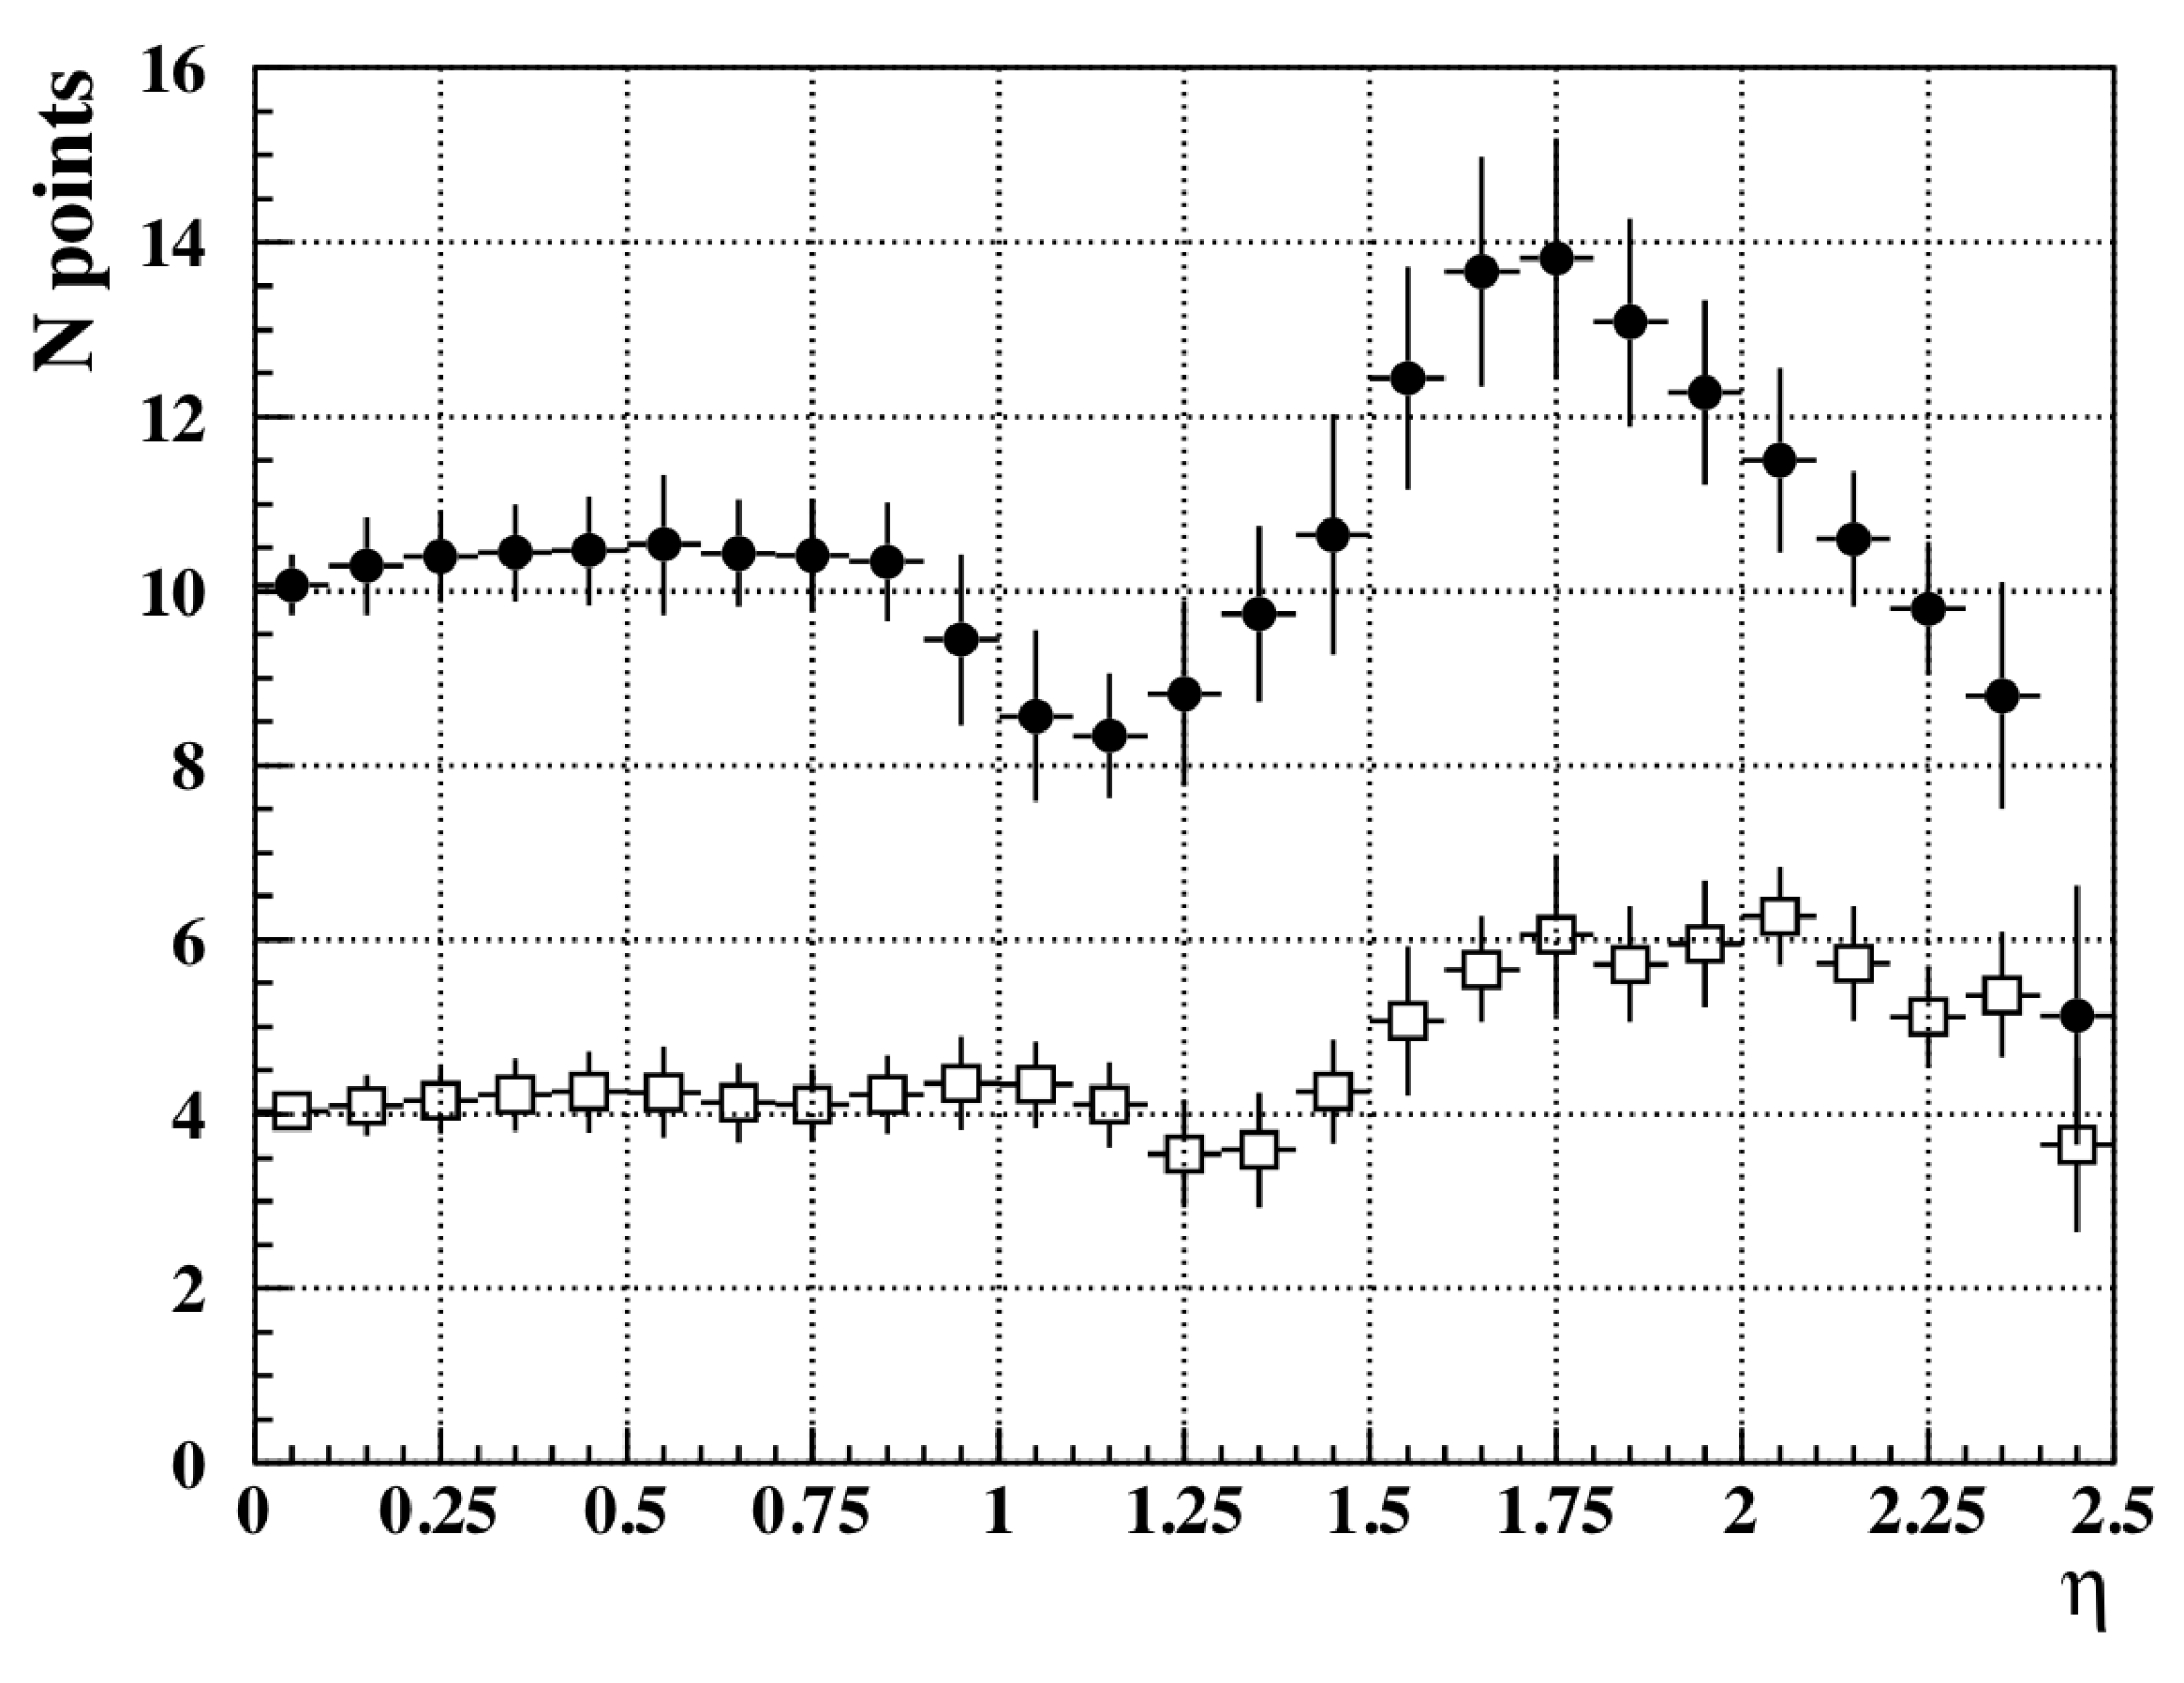
\includegraphics[width=0.55\textwidth]{nhits.pdf}
\caption[
Radiation length and number of layers crossed in the CMS tracker as a function
of pseudorapidity.
]{ \label{fig:cms_material}
Radiation length of the CMS tracker as a function of pseudorapidity
(left). Number of layers passed as a function of
pseudorapidity (right). Black circles represent total layers while hollow
squares represent the number of layers with a stereo measurement~\cite{trackingperformance}.
}
\end{center}
\end{figure}
% --------------------------------------------------------------------------- %

The tracker provides at least ten particle position measurement for any
possible particle trajectory within the tracker's acceptance region
which is about $\aeta < 2.5$. Figure~\ref{fig:cms_material} shows the
number of measurements as a function of $\aeta$. Some of the tracker's
silicon layers have duel layers with a slight offset to facilite a more
accurate positional measured. The number of these stereo layers are also
shown in Figure~\ref{fig:cms_material}. The overall initial transverse
position (traverse impact parameter, \dzero) and the momentum resolution
is shown in Figure~\ref{fig:cms_tkres}. The overall charged particle
reconstruction efficiency, calculated using standard tag and probe
techniques (see Section~\ref{sec:eff_tnp}), is on average greater than
99\%~\cite{trackingperformance}.

% --------------------------------------------------------------------------- %
\begin{figure}[!htb]
\begin{center}
\subfloat{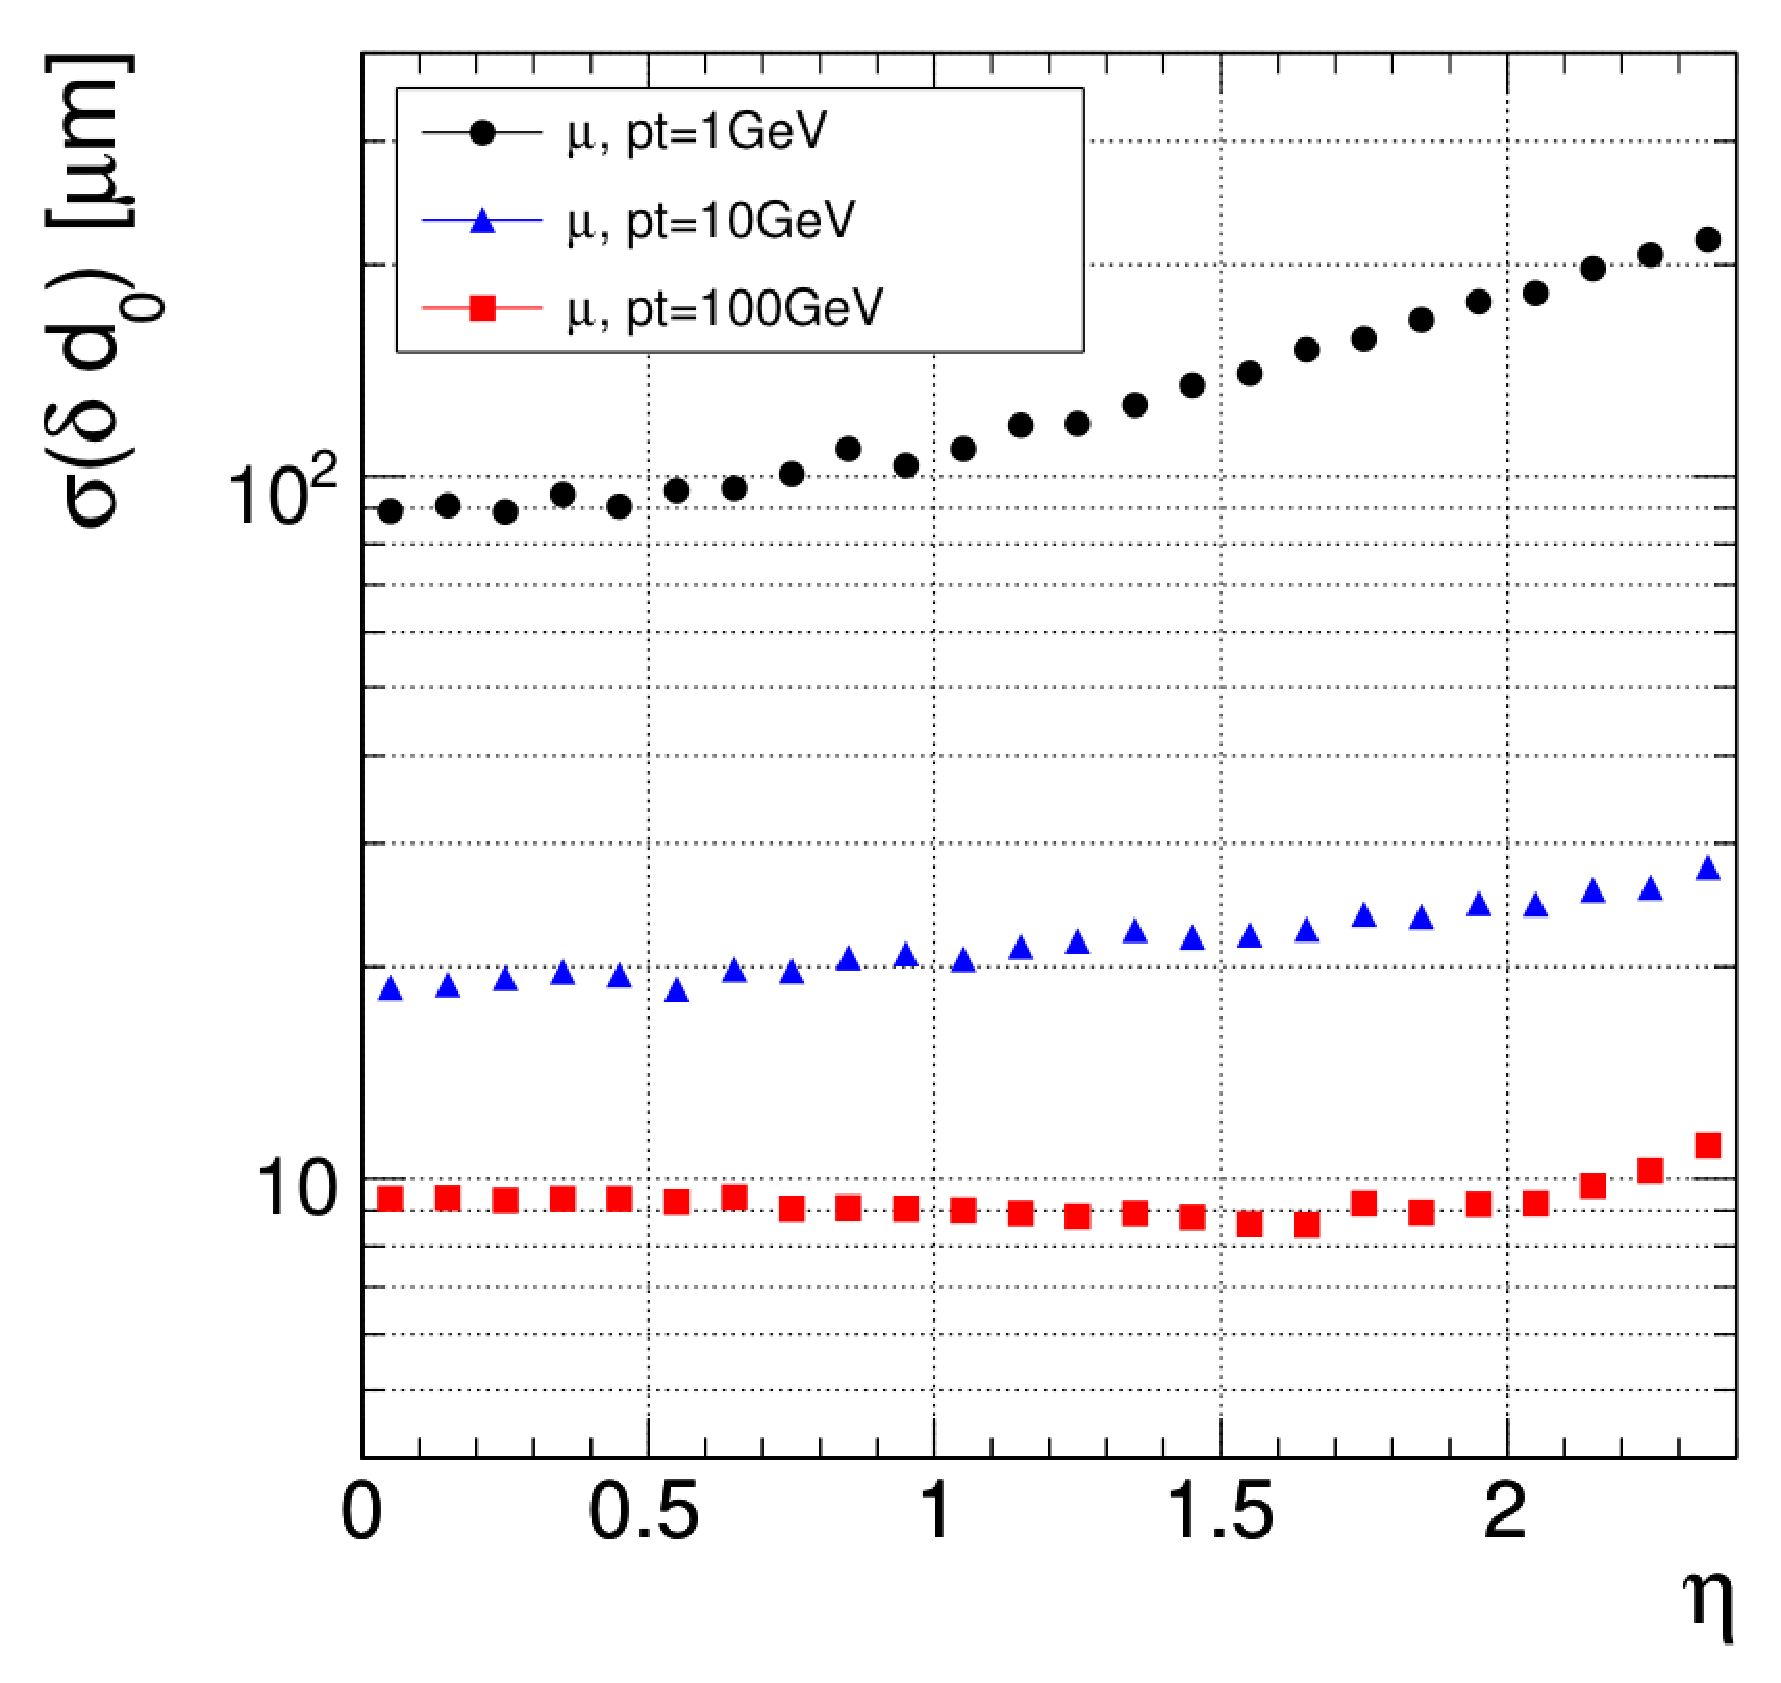
\includegraphics[width=0.45\textwidth]{d0resveta.pdf}} 
\subfloat{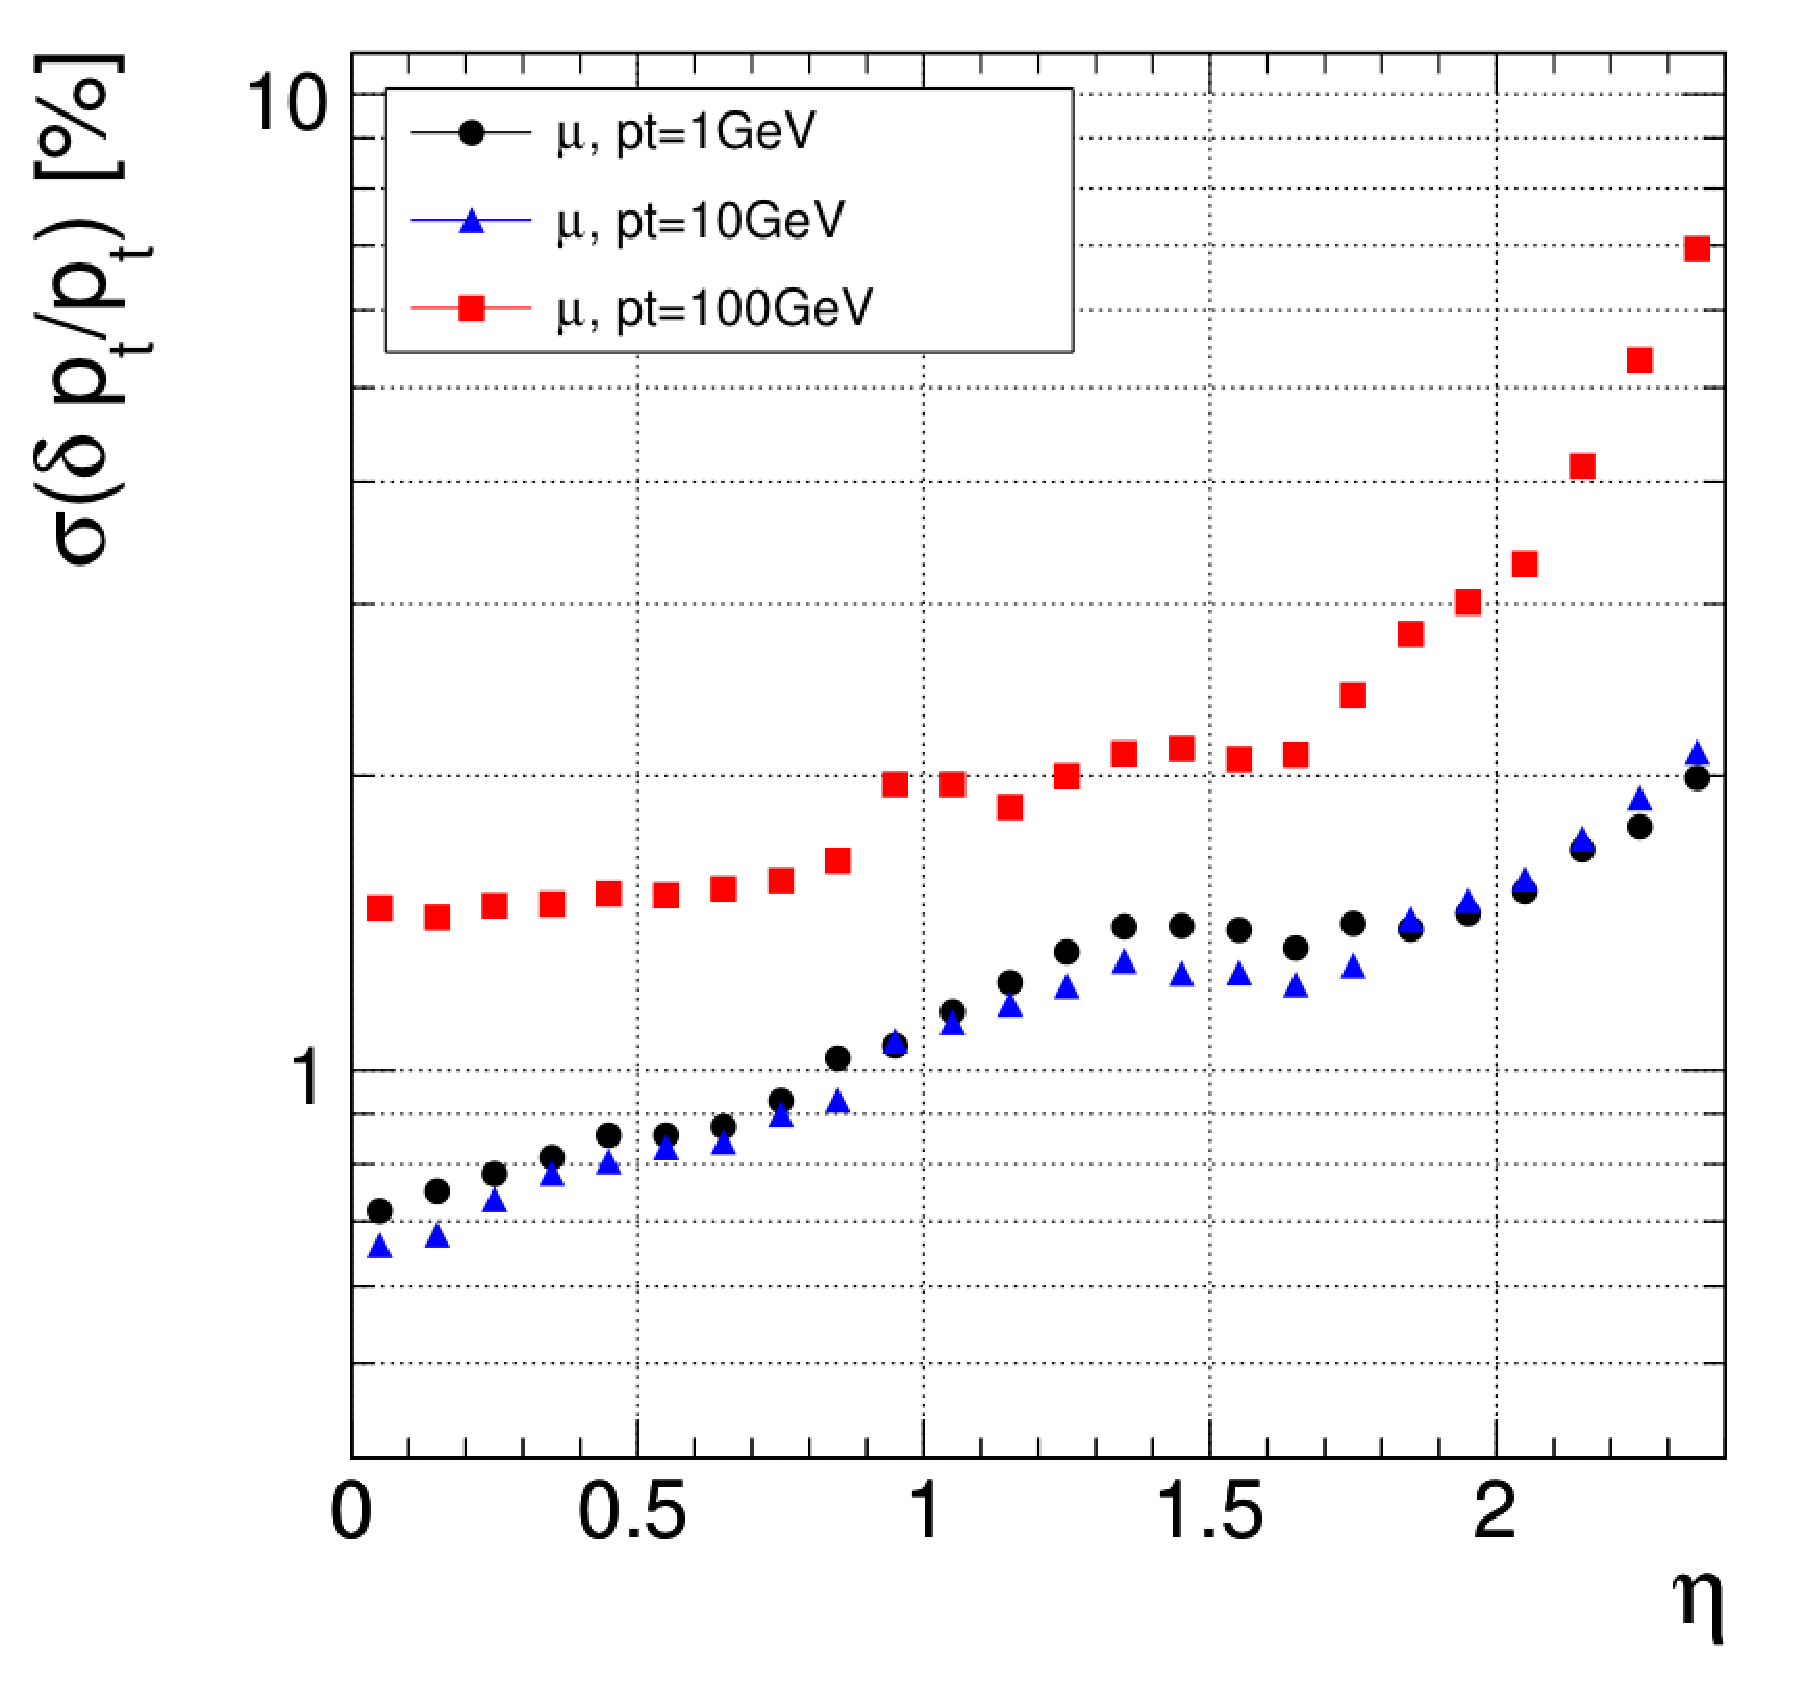
\includegraphics[width=0.45\textwidth]{ptresveta.pdf}}
\caption[
Muon transverse impact parameter resolution and transverse momentum
resolution as a function of pseudorapidity
]{\label{fig:cms_tkres}
Muon transverse impact parameter
resolution (left) and transverse momentum resolution as a function of
pseudorapidity for various muon momenta: 1 \GeV as circles, 10 \GeV as
triangles and 100 \GeV as squares~\cite{trackingperformance}.
}
\end{center}
\end{figure} 
% --------------------------------------------------------------------------- %

% --------------------------------------------------------------------------- %
% --------------------------------------------------------------------------- %
\subsection{The Calorimeters}
\label {sec:cms_calo}
% --------------------------------------------------------------------------- %
% --------------------------------------------------------------------------- %
CMS has two calorimetry detectors, both situated inside the solenoid. The
first, directly behind the silicon tracker, is the electromagnetic calorimeter
(ECAL), designed to measure the energy of particles which interact primarily
electromagnetically, i.e. electrons and photons. The second, directly behind
the ECAL, is the hadronic calorimeter (HCAL), designed to measure particles
interacting predominately by the strong interaction. Both sub-detectors were
designed to be fully hermetic, have good energy resolution over a large
area of the detector, and hence be able to accurately reconstruct the total
amount of energy released for each proton-proton interaction. Combined, the
calorimeters allow for the detection of neutrinos escaping from the CMS
detector by measuring an energy imbalance in the transverse plane. In addition,
the calorimeters are designed to be thick enough to prevent most particles
from pushing through the solenoid and into the muon chambers. To achieve these
features, both detectors had to be composed of dense and highly segmented
material.

\subsubsection{Electromagnetic Calorimeter}
\label {sec:cms_ecal}

Lead Tungstate (\pbw) crystals were chosen to comprise the fully hermetic and
homogeneous ECAL. \pbw satisfies the needs imposed by the LHC environment: the
radiation resistance allows for long lifetime and the high density satisfies
the space constraints as well as allows for fine granularity and quick read
out times. The homogeneity of the detector allows for good overall energy
resolution. \pbw has a radiation length ($X_0$) of 0.89 \cm and a Moli\`ere
radius of 2.2 \cm. The Moli\`ere radius is a measure of the spread of energy
from showering electrons and photons and is defined as the radius which
contains 90\% of the showering energy. Having a small Moli\`ere radius also
allows for the use of smaller crystals and hence gives higher segmentation.
Finally, \pbw has a quick scintillation decay time which allows for read out
times fast enough to deal with the signed 25 ns interaction spacing of the LHC.

The ECAL barrel (EB) contains 61,200 \pbw crystals arranged in a cylindrical
formation around the silicon tracker. Each crystal is rectangular in shape, 240
mm long ($\sim 26 X_0$), $22 \times 22$ $\rm{mm^2}$ on the front surface and
$26 \times 26$ $\rm{mm^2}$ on the near surface. The EB cover a pseudorapidity
range $\aeta < 1.479$ with each crystal having a size in $\eta - \phi$ space of
$0.0174 \times 0.0174$.

The ECAL endcaps (EE+ and EE-) each contain 7,324 \pbw crystals and cover
pseudorapidity range of $1.479 < \aeta < 3.0$. Each EE is split into an upper
and lower disk, ``dees'' which arrange the crystals in an $x - y$ pattern while
situating the crystal face to point in the direction of the nominal interaction
point. The crystals are approximately $30 \times 30$ mm on their face with a
length of 220 $\rm{mm^2}$ ($\sim 25 X_0$).

In addition to the EB and EE, there is an additional electromagnetic calorimeter
stationed on each side directly in front of the EE. Called the preshower (ES),
this sub-detector gives additional radiation lengths and helps differentiate
electrons and photons from pions. A full schematic of the ECAL system can be
seen in Figure~\ref{fig:cms_ecal}.

% --------------------------------------------------------------------------- %
\begin{figure}[!htb]
\begin{center}
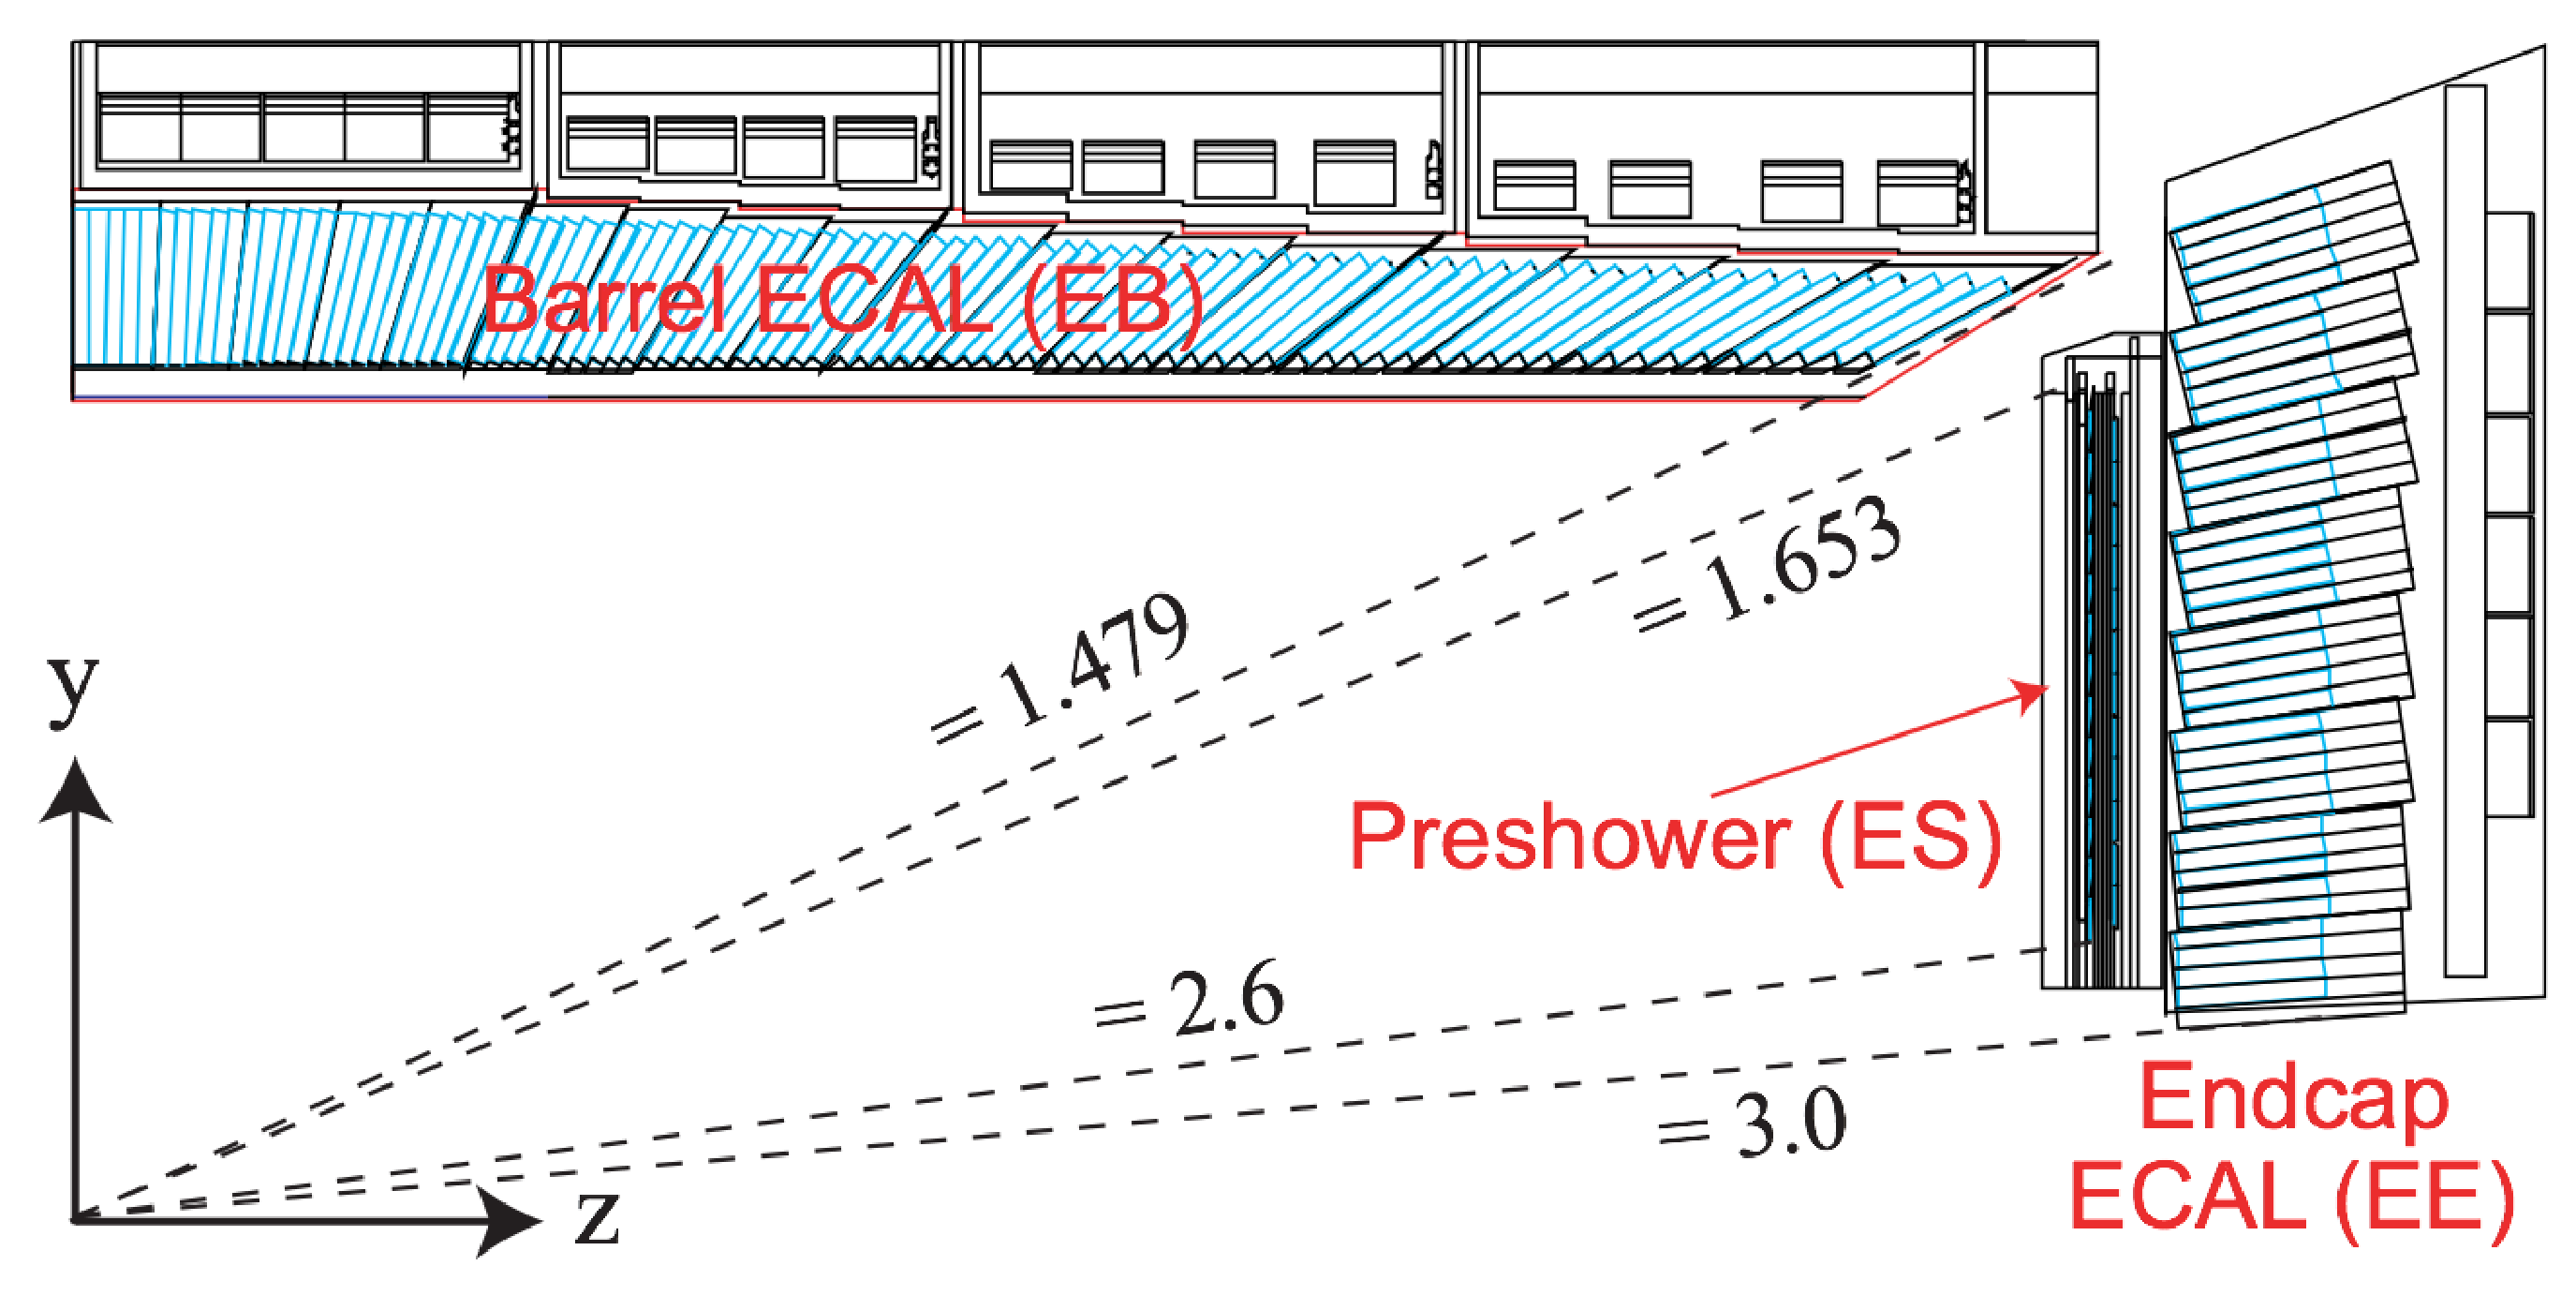
\includegraphics[width=0.8\textwidth]{ecal.pdf}
\caption{\label{fig:cms_ecal}
One quarter of the electromagnetic calorimeter system projected into the $y-z$
plane~\cite{tdr1}.
}
\end{center}
\end{figure}
% --------------------------------------------------------------------------- %

To convert the light created in the crystals to an electrical signal, silicon
avalanche diodes (APDs) and vacuum phototriodes (VPDs) are used in the barrel
and endcap, respectively. Both photo-detectors were designed to be fast, have a
high radiation tolerance and be able to operate in the presence of CMS's strong
magnetic field. In addition, the photo-detectors have to be able to withstand
the bombardment of hadronic particles passing through their active area without
too much disruption and to be able to amplify the low light output of the \pbw
crystals.

\subsubsection{Hadronic Calorimeter}
\label {sec:cms_hcal}

The HCAL sits between the ECAL and the solenoid and is important for the
identification and reconstruction of hadronic energy~\cite{hcalperformance}.
The HCAL is comprised of four different sets of sub-detectors, the HCAL barrel
(HB), the HCAL endcaps (HE), the outer HCAL (HO), and the forward HCAL (HF). A
full schematic of the HCAL system can be seen in Figure~\ref{fig:cms_hcal}.

% --------------------------------------------------------------------------- %
\begin{figure}[!htb]
\begin{center}
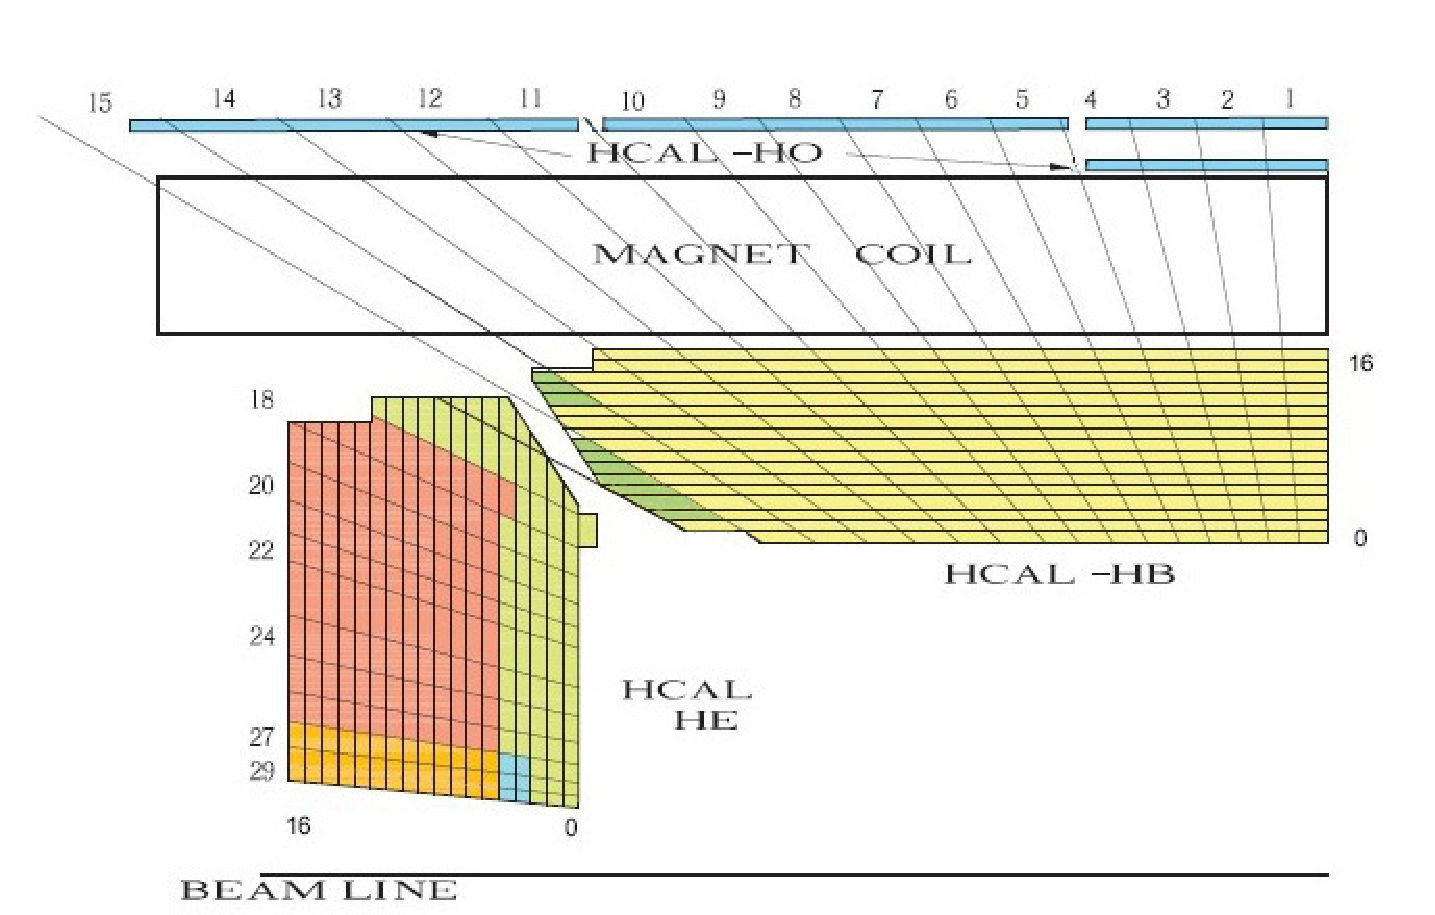
\includegraphics[width=0.9\textwidth]{hcal.pdf}
\caption{\label{fig:cms_hcal}
One quarter of the hadronic calorimeter system projected into the $y-z$
plane~\cite{hcalperformance}.
}
\end{center}
\end{figure}
% --------------------------------------------------------------------------- %

The HB and HE both use brass alloy (70\% Cu, 30\% Zn), which has an interaction
length ($\lambda_I$) of 15 \cm. This ensures as much hadronic showering as
possible while still falling within the spatial and monetary constraints. The
HB covers the \pr range of $\aeta < 1.3$ and contains 36 wedge shaped blocks of
material (18 around the cylinder and each half of the HB). Each wedge consists
of a flat brass absorber plate that runs parallel to the beam axis with plastic
scintillators interspersed throughout, which convert the hadronizing energy
into light for detection. The scintillators are distributed to give a spacial
segmentation of $0.087 \times 0.087$ in $\eta - \phi$ space. The interaction
length of the HB varies from 5.92 to 10.6 $\lambda_I$, depending on the \pr.
The HE takes over where the HB leaves off and covers a \pr range of $1.3 <
\aeta < 3.0$. The granularity in this region allows for positional measurements
with a size of $0.087 \times 0.087$ up to $\eta < 1.6$ and $0.17 \times 0.17$
beyond $\aeta > 1.6$. The total depth of the HE is nine interaction lengths.
Both the HB and HE utilize multipixel hybrid photodiodes (HPD), which operate
well in strong magnetic fields, to convert the scintillator light to an
electric signal.

Between $3.0 < \aeta < 5.0$ sits the HF which, instead of brass, uses steel to
absorb the hadronic particles. Due to the very large particle fluxes in this
region, scintillators were replaced by more radiation hard quartz fibers.
These quartz fibers emit Cherenkov radiation which is then channeled to the
readout photodiodes. The segmentation of the HF gives the approximate size
of each readout channel as $0.18 \times 0.18$ in $\eta - \phi$ space.

Finally, to supplement the energy measurement in the barrel, the region with
the lowest interaction length, the HO sits outside the solenoid. In fact,
it uses the solenoid as an extra absorber material, which gives at least
1.5 interaction lengths, depending on the \pr. The HO utilizes scintillator
material directly behind the solenoid to measure the energy of any particle
which hadronizes inside the solenoid. With the ECAL giving approximately one
interaction length, the total interaction length of CMS is always greater
than 11.8, giving $< 0.1\%$ chance of a hadron punching through to the muon
detectors.

% --------------------------------------------------------------------------- %
% --------------------------------------------------------------------------- %
\subsection{The Muon Detectors}
\label {sec:cms_musys}
% --------------------------------------------------------------------------- %
% --------------------------------------------------------------------------- %
The Compact Muon Solenoid was designed to efficiently and precisely detect
muons. Muons, unlike the much lighter and radiative electrons, interact very
minimally with matter, traversing even the densest parts of CMS (the ECAL and
HCAL) with relative ease while at the same time depositing very little of its
energy. Muons are also relatively long lived and their lifetime allows them to
be measured by the CMS detector before it decays. It is for these reasons that
the muon detectors are situated outside the solenoid, far from the interaction
point.

The muon system employs three different gas-based particle detectors which
allow for excellent muon measuring capabilities. In addition to positional
measurements, the muon detectors also provide muon identification, momentum
and triggering (see Section~\ref{sec:cms_daq}). The chambers sit inside CMS's
iron return yoke which acts as an absorbing material for hadrons and other
non-muon particles which try to penetrate through the solenoid. In the barrel,
the drift tube (DT) sub-detector sits cylindrically concentric. The endcap
houses cathode strip chambers (CSC) which consist of four layers on each side
of the barrel. Finally, interspersed through the barrel and endcap, is the
resistive plate chambers (RPC) used to enhance the timing resolution of the
detection of muons. A graphical overview of the CMS muon system is shown in
Figure~\ref{fig:cms_musys}.

% --------------------------------------------------------------------------- %
\begin{figure}[!hbt]
\begin{center}
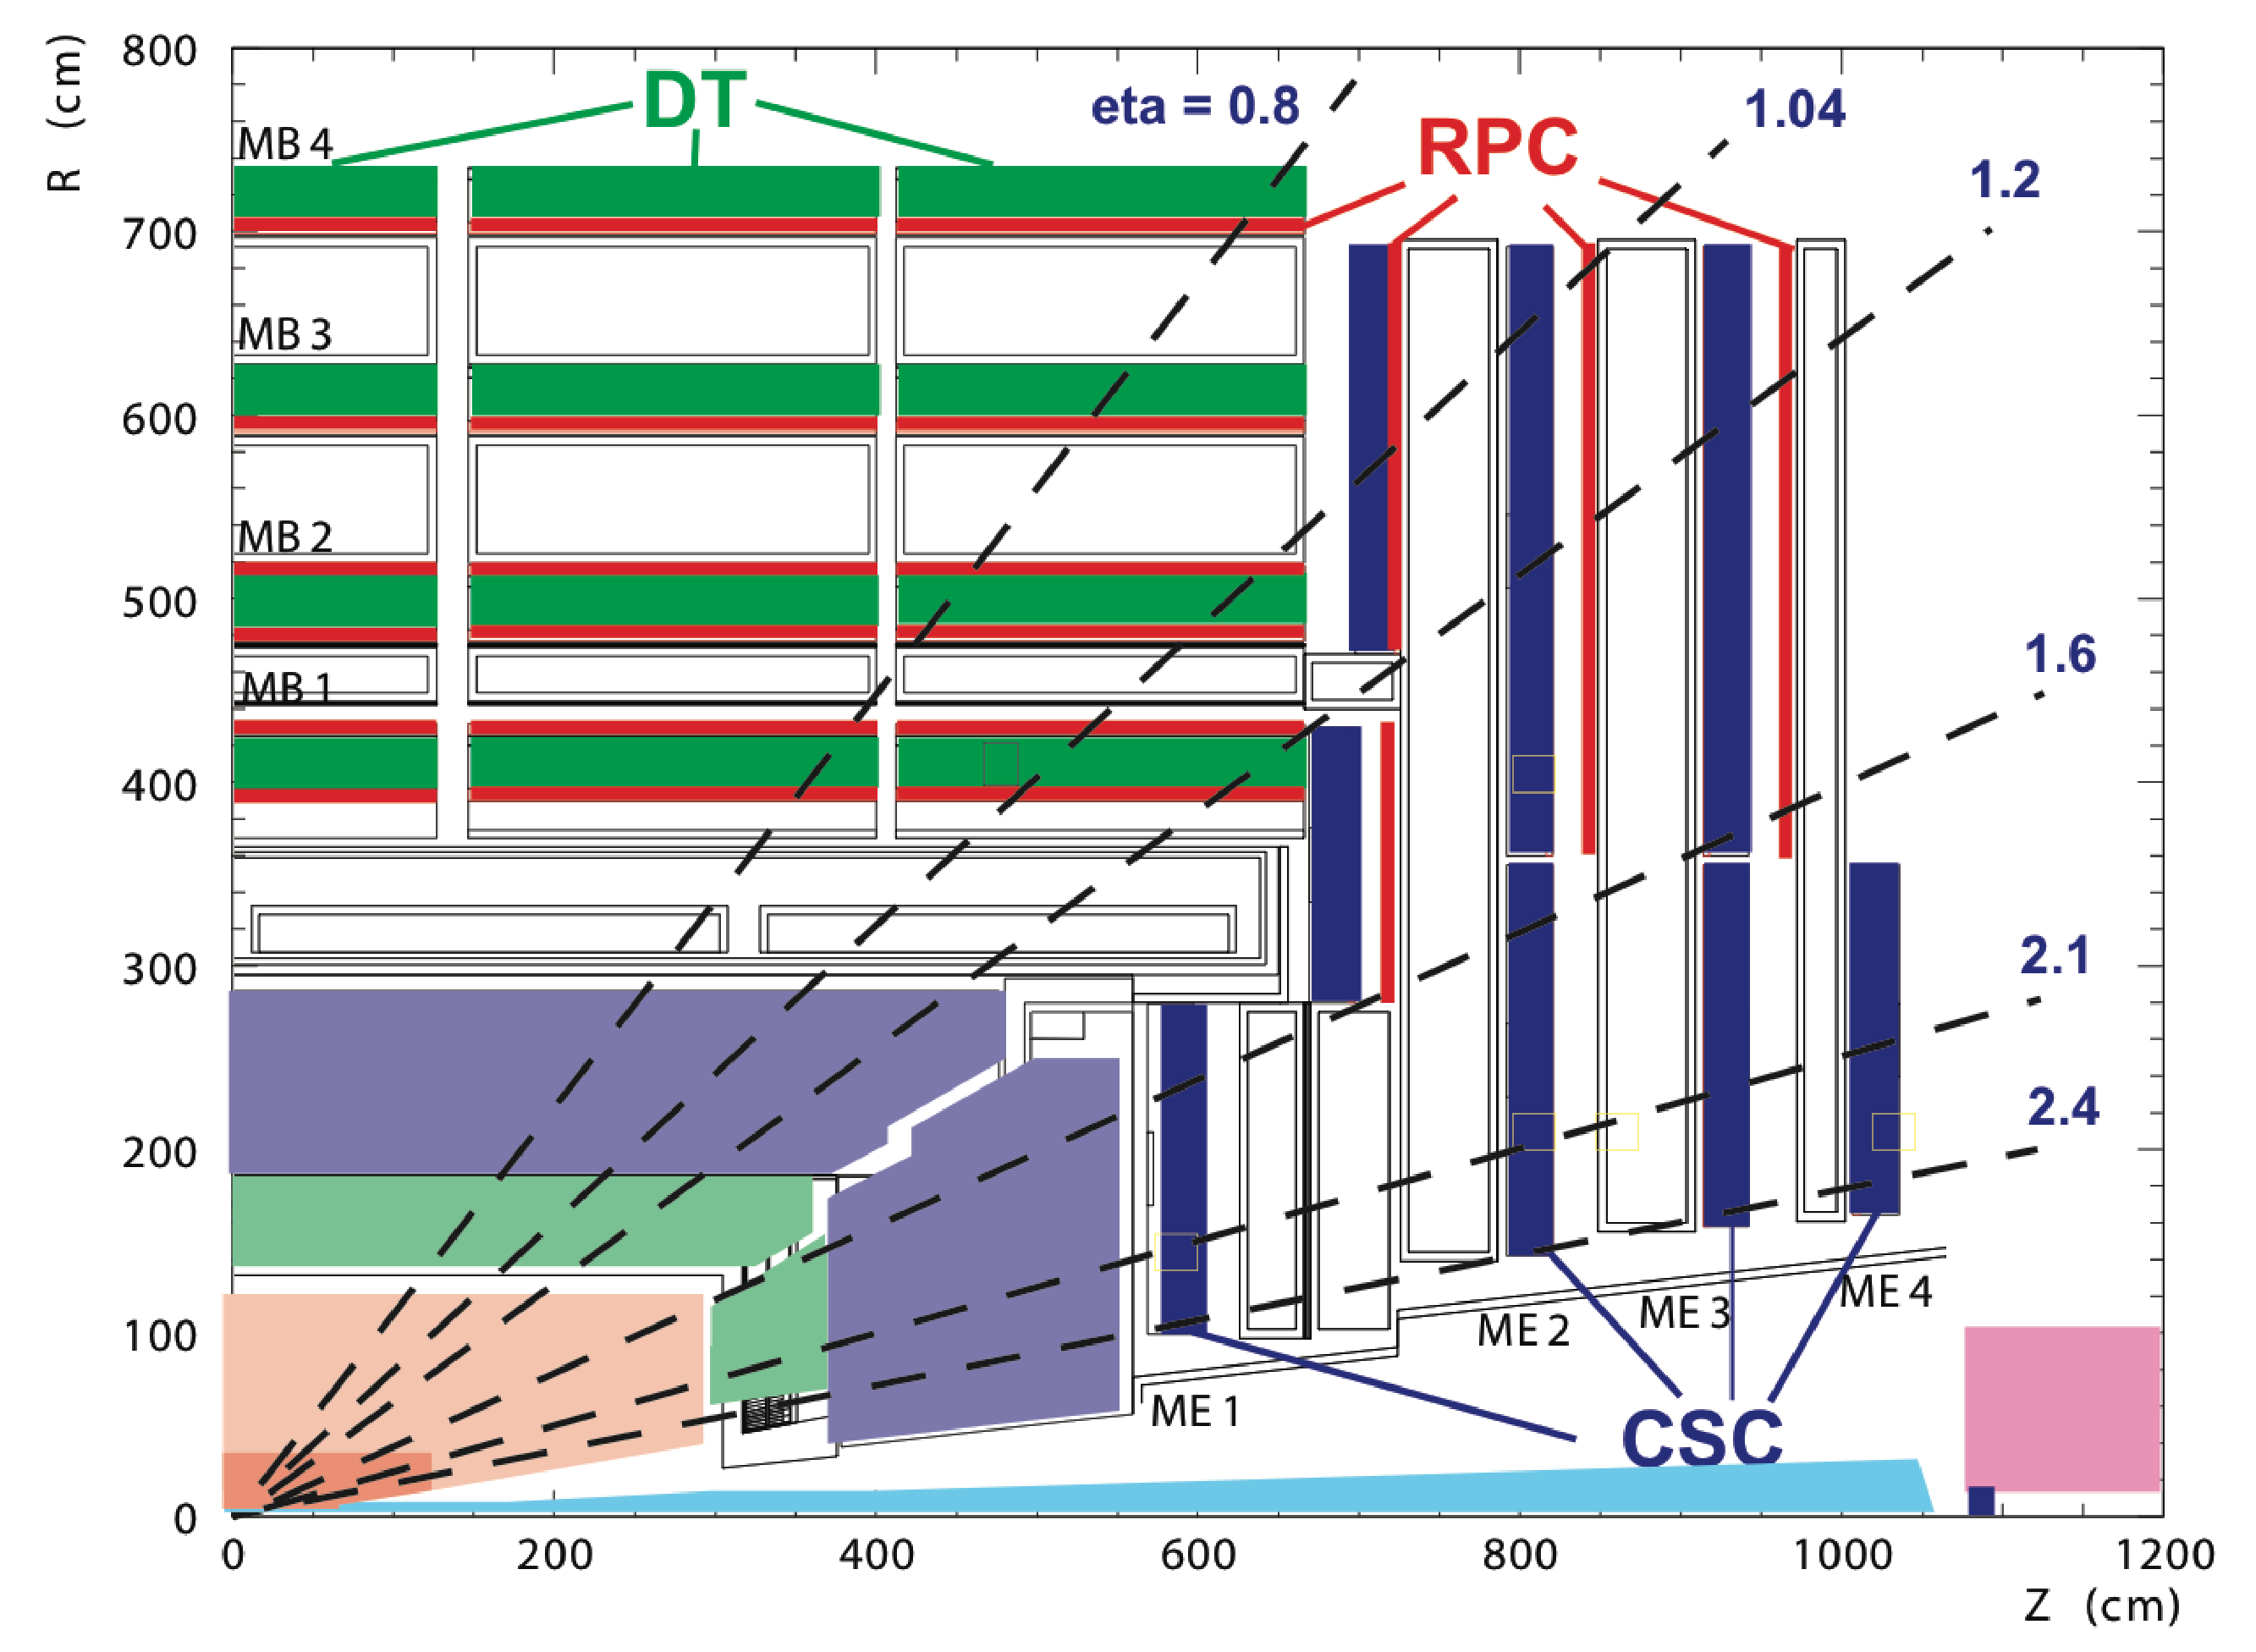
\includegraphics[width=0.8\textwidth]{musys.pdf}
\caption[Overview of the CMS muon subdetector system]
{\label{fig:cms_musys}
Overview of the CMS muon sub-detector system. The drift tubes, situated in the
barrel region, are shown in green, the cathode strip chambers, situated in the
endcap region, are shown in blue and the resistive plate chambers, situated
throughout, are shown in red~\cite{muontdr}.
}
\end{center}
\end{figure}
% --------------------------------------------------------------------------- %

\subsubsection{Drift Tubes}
\label {sec:cms_musys_dt}

Drift tubes are long cylindrical tubes filled with gas and threaded with an
equally long conductive wire (the anode). The inside of the cylinder is also
lined with a conductive material (the cathode). The gas, a mixture of noble gas
with full set of valence electrons, relinquishes electrons as charged particles
traverse through it. A bias voltage is applied across the wire and the cylinder
causing the electrons to flow one way and particle detection is achieved through
measuring the amount of induced current.

The DT system sits in the barrel region outside the solenoid and
covers a \pr range $\aeta < 1.2$. Each set of drift tubes are arranged as a
rectangular chamber and staggered throughout the return yoke. There are 250
chambers arranged in four concentric cylinders of chambers (stations) divided
by five rings (wheels) of the return yoke. The chambers have a slight overlap
to ensure the hermeticity in 12 different sectors of each ring and wheel, each
covering $30^{\circ}$ in azimuthal angle. The four stations and two and a half
of the wheels can be seen in green in Figure~\ref{fig:cms_musys}.

Each chamber except the last has three sets (superlayers) of four planes
of drift tubes. Tow of the superlayers in each chamber run parallel to the
beam direction to measure the $r-\phi$ position. The third superlayer in the
first three chambers have drift tubes that run perpendicular to the beam line
allowing an additional measurement in the z-direction.

In all, there are over 172,000 drift tubes in the DT system each with an
approximate length of 2.5 m. This length, coupled with the low background and
muon rates and the uniform magnetic field in this region of the detector allow
for the one-dimensional position measurements of the DT system. The DT's give a
time resolution of $\sim$25 ns, well within the timing constraints of the LHC,
and a global resolution in the $r-\phi$ direction of 100 \um.

\subsubsection{Cathode Strip Chambers}
\label {sec:cms_musys_csc}

A cathode strip chamber is similar to a drift tube chamber in that it is
a gaseous detector filled with anode wires; however, instead of a wire
tube per cathode tube, the anode wires are stretched in parallel and are
surrounded on either side by a plan of cathode material. One plane of the
cathode is segmented into strips which run perpendicular to the anode wires.
The induced charge distribution on the wires and strips gives a fully
two-dimensional measurement of a passing particle (in addition to the third
known position given by the position of the chamber). In addition to giving a
three-dimensional positional measurements, the CSCs were also designed with a
fast response time, fine segmentation and to be radiation hard in order to deal
with increased background and muon rates and the non-uniform magnetic field in
the endcap region (as opposed to the lower rates in the barrel where positional
ambiguity can be tolerated).

The CSCs operate in the \pr region $0.9 < \aeta < 2.4$. Similar to the
barrel, there are four stations in each endcap region, arranged in radial
disks perpendicular to the beam line. There are 468 chambers in total, each
trapezoidal in shape and arranged side-by-side circularly around the beam line
in two concentric circles. The anode wires run along the azimuthal direction
and provide the radial measurement while the strips run lengthwise in a radial
direction and give a measurement in $\phi$. The overall positional resolution
of the CSC is between 75 and 150 \um. The CSC system is shown in blue in
Figure~\ref{fig:cms_musys}.

\subsubsection{Resistive Plate Chambers}
\label {sec:cms_musys_rpc}

The goal of the RPC muon detector system is to compliment the CSCs and DTs
by adding faster readout times at the expense of position resolution. The
RPC chambers consist of two gaseous regions separated by a common
strip readout anode plane which gives adequate positional resolution.
Operating with a time resolution well below the minimum of 25 ns,
the RPCs are ideal detectors to be used to ``trigger'', the CMS detector
(see Section~\ref{sec:cms_daq}). The RPC system covers a \pr range of
$\aeta < 1.6$. Originally designed to cover the full range, it will be
completed during the next upgrade. The RPC chambers can be seen in red in
Figure~\ref{fig:cms_musys}. Running along the beam direction (and hence
measuring the azimuthal angle), six (three) layers of chambers exist in the
barrel (endcap) with over 480 chambers in total each approximately 2.5 meters
in length.

\subsubsection{Summary}
\label {sec:cms_musys_summary}

Overall, the muon system was designed to have an efficiency of over 95\% for
detecting muons with a resolution of less that 10\% for muons up to $\pt =
200 GeV$, increasing with resolution between 15\% and 40\% for 200 \GeV to 1
\TeV muons (depending on \aeta). Using the tracker as an additional set of
measurements on the muon, the expected resolution improves to around 1\% for
lower \pt muons and down to approximately 5\% for muon in the TeV range. The
expected resolution on the transverse momentum measurement can be seen for two
different \pr ranges in Figure~\ref{fig:cms_mures}.

% --------------------------------------------------------------------------- %
\begin{figure}[tbhp]
\begin{center}
\subfloat{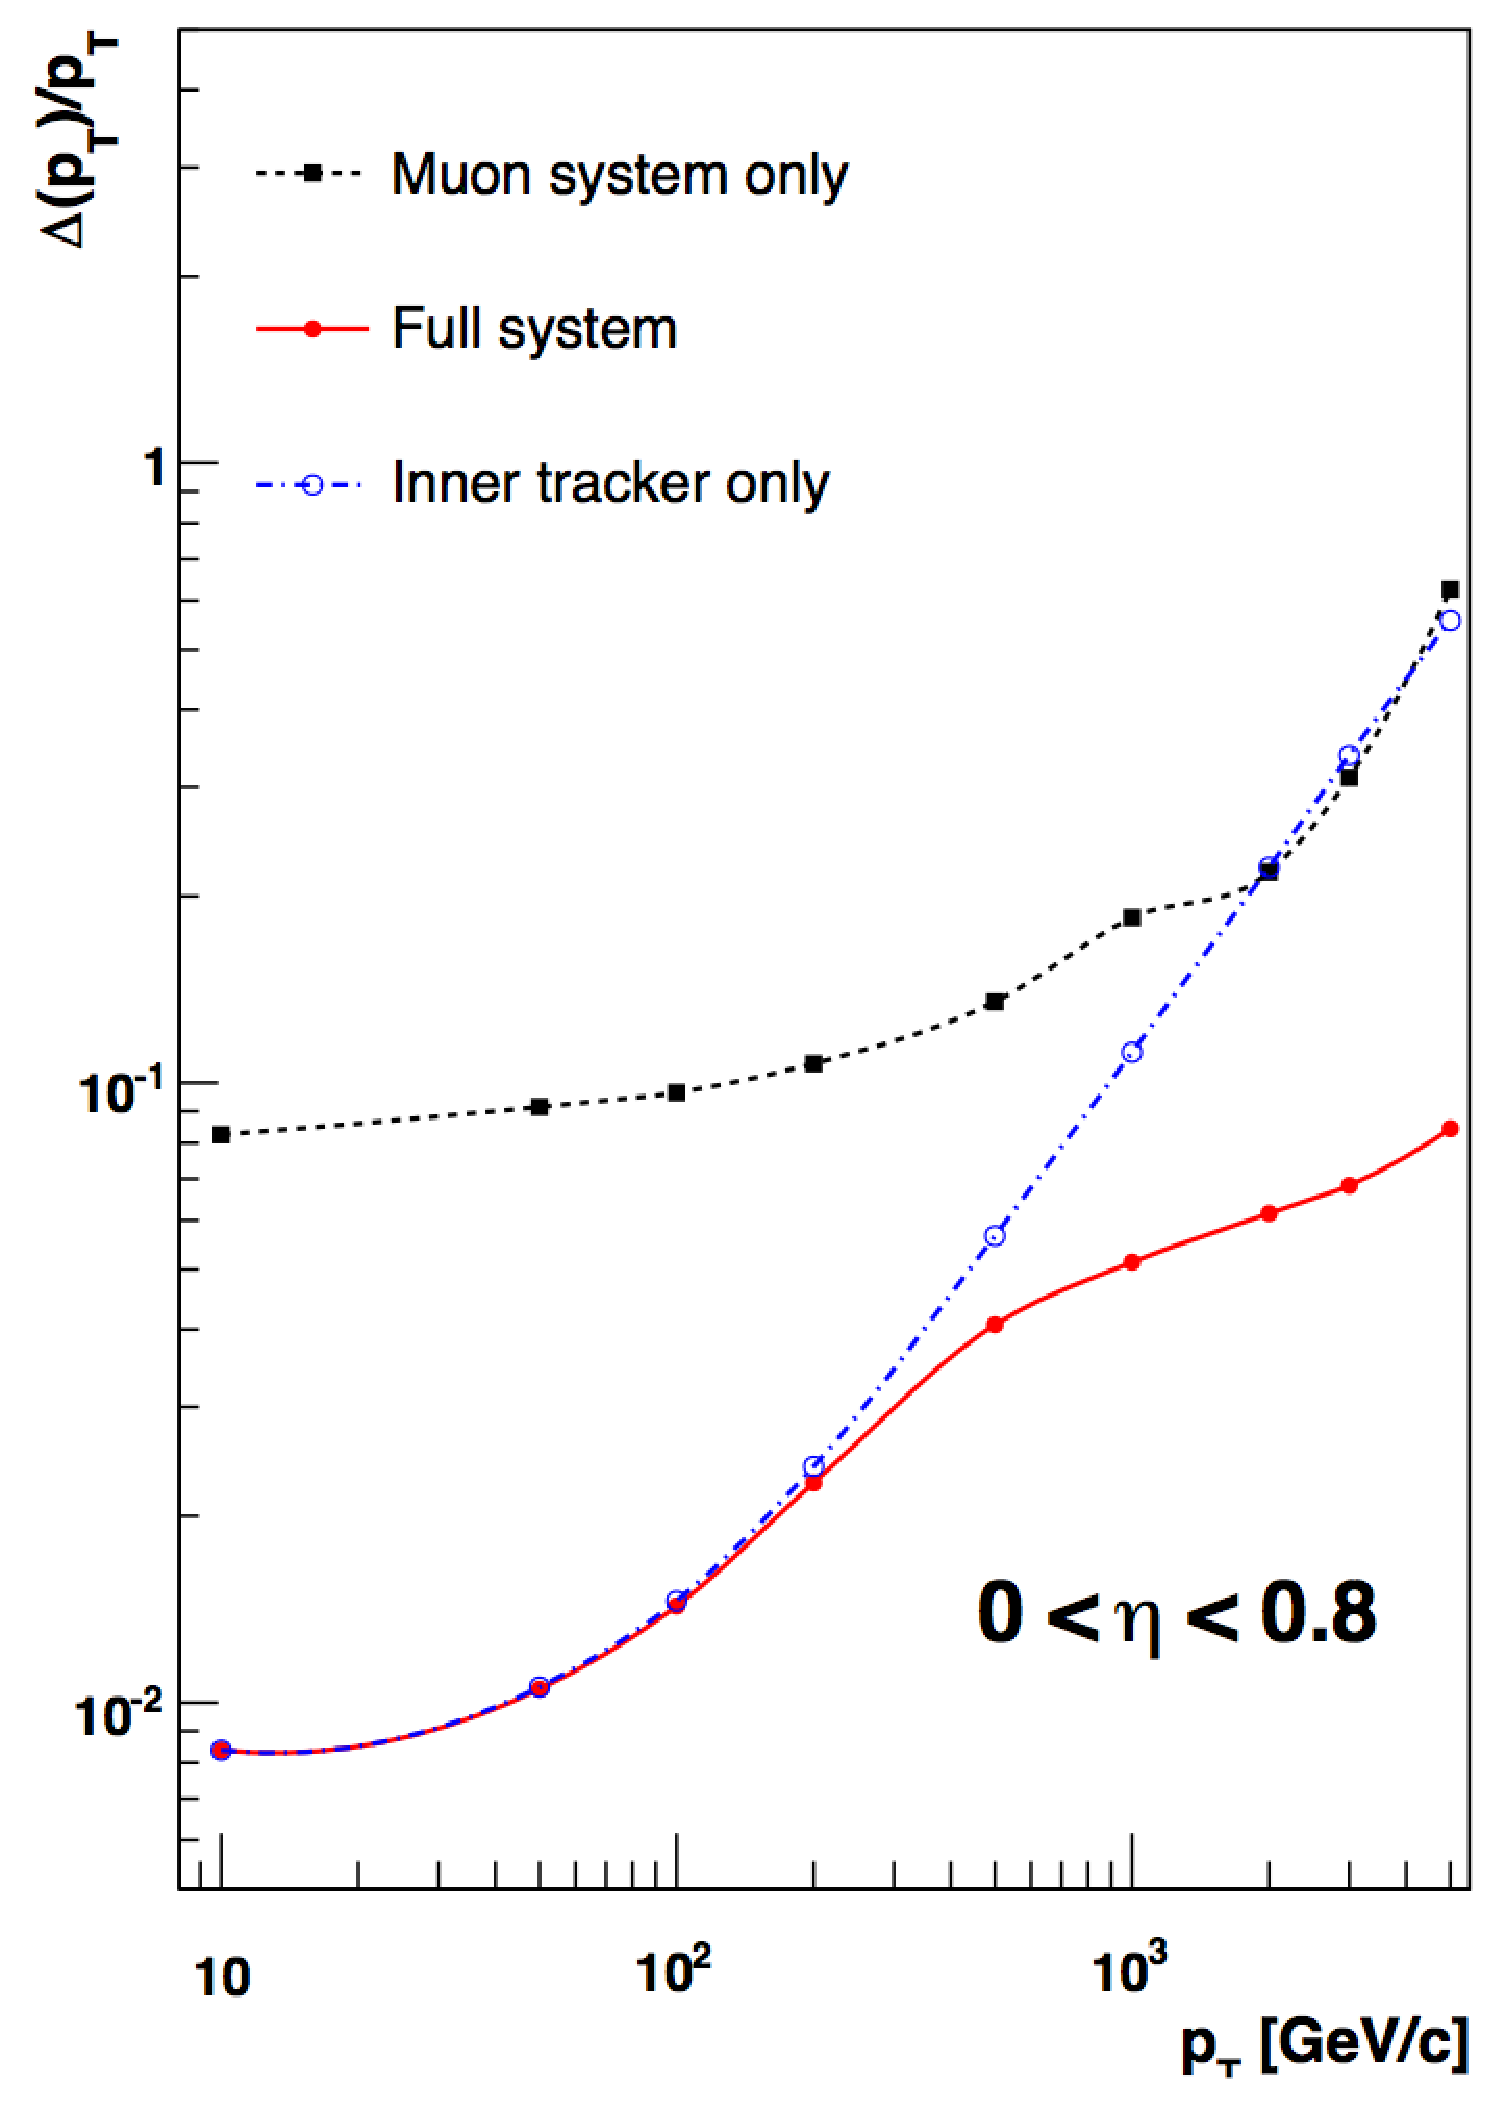
\includegraphics[width=0.40\textwidth]{muresloweta.pdf}} \hspace{5mm}
\subfloat{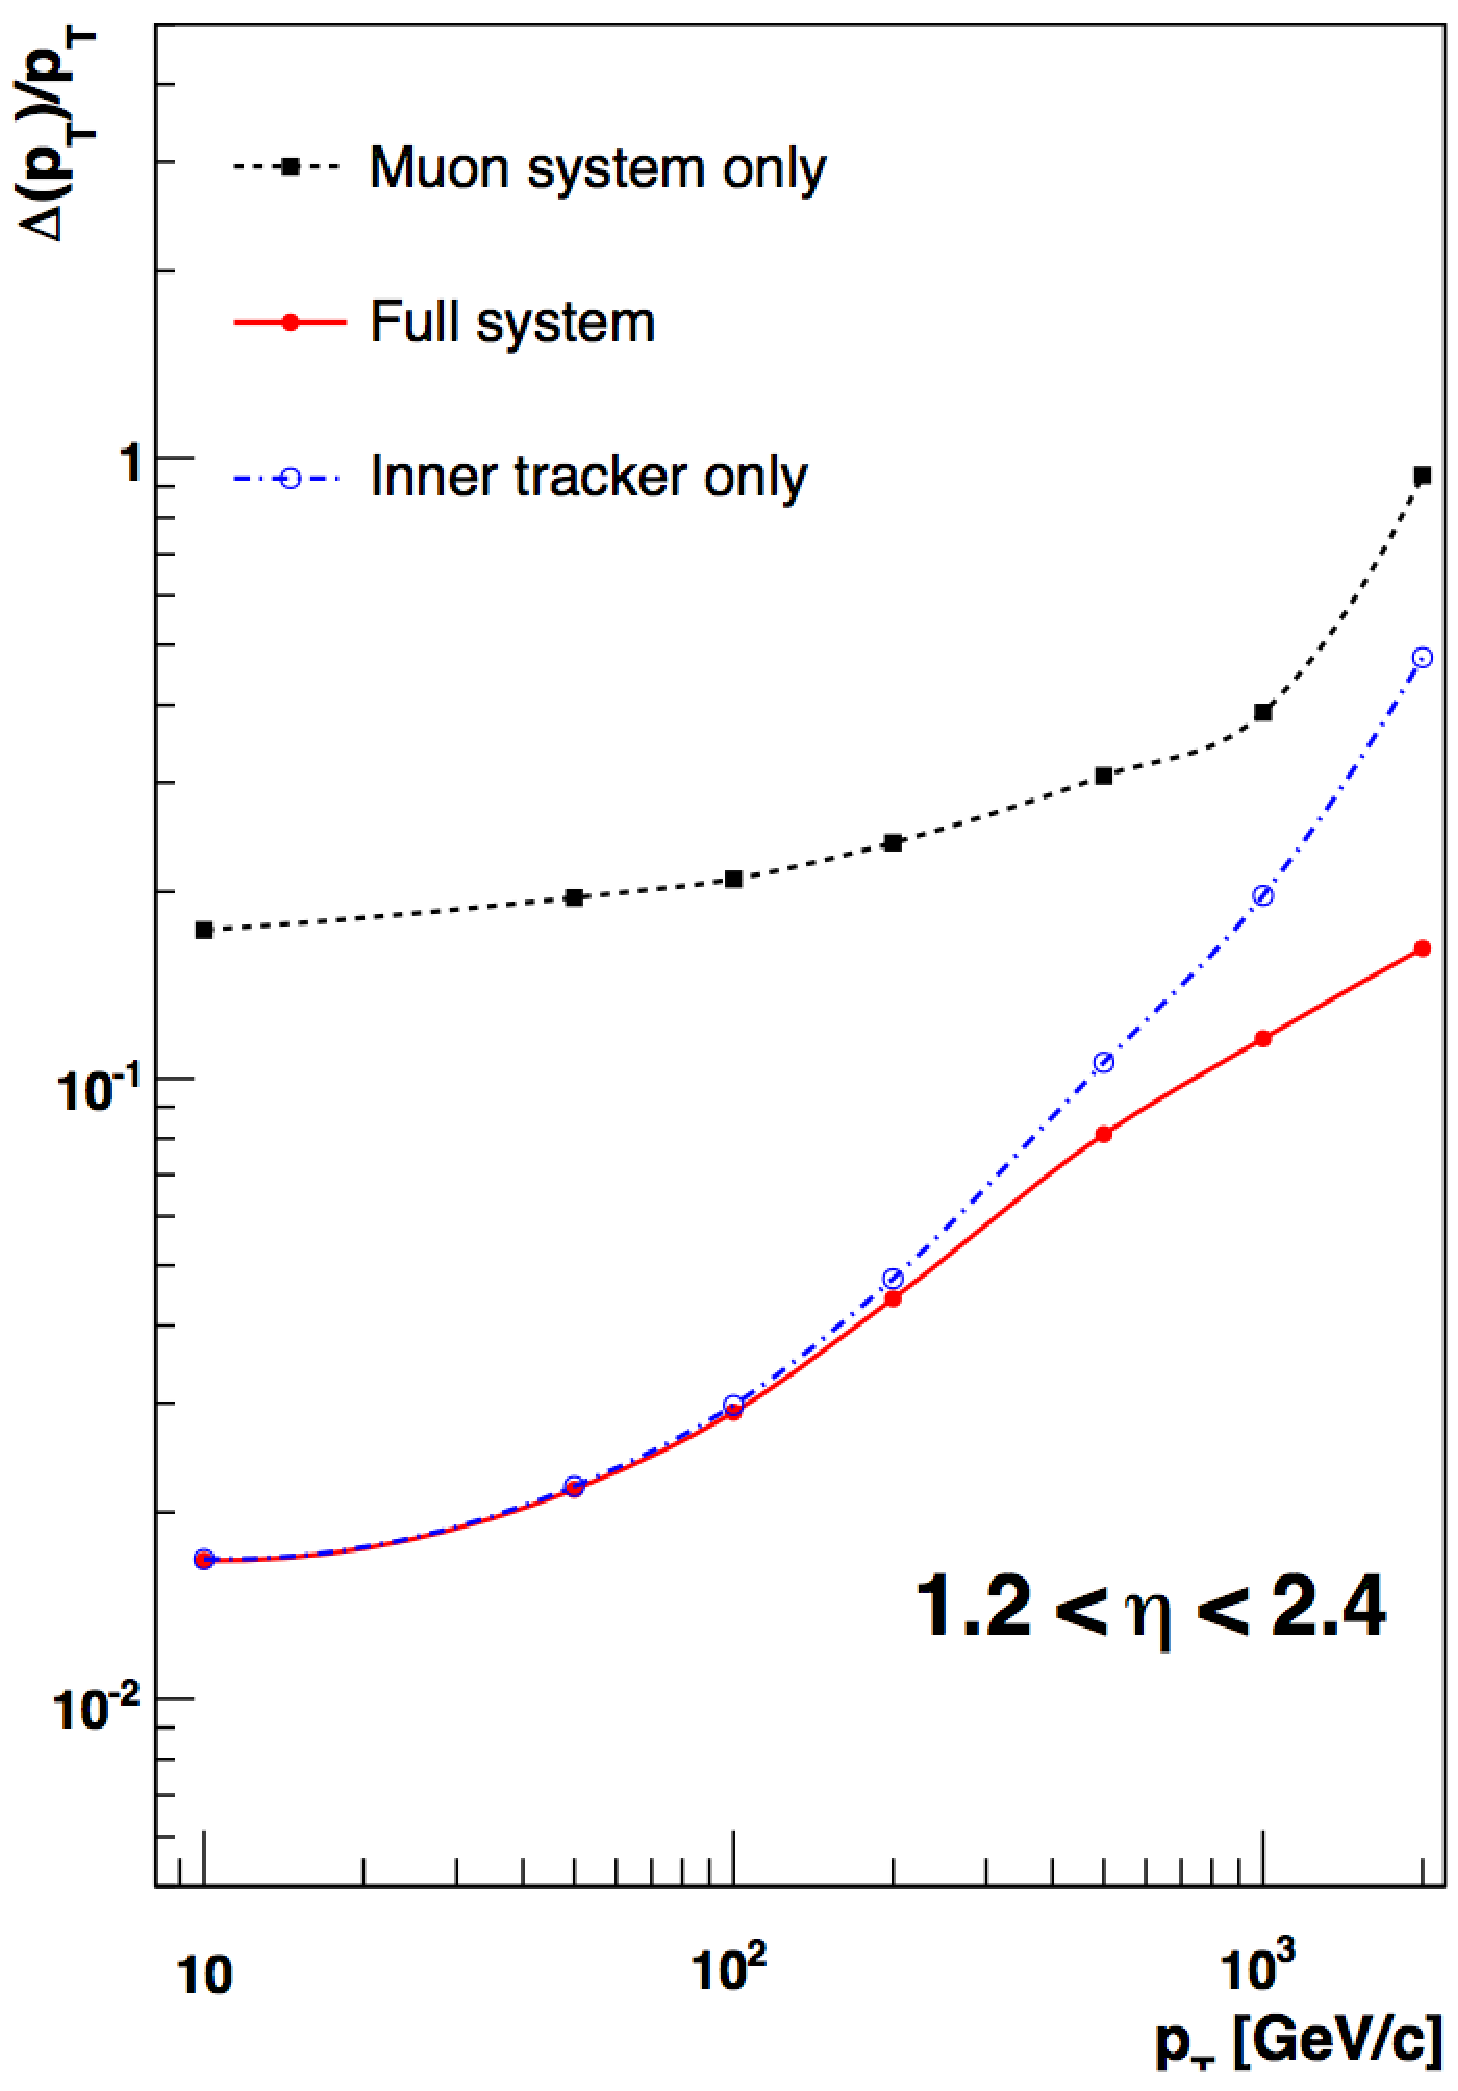
\includegraphics[width=0.39\textwidth]{mureshigheta.pdf}} \\
\caption[Muon momentum resolution for two different pseudorapidity regions]
{\label{fig:cms_mures}
Muon momentum resolution for two different pseudorapidity regions, $0< \aeta
<0.8$ (left) $1.2< \aeta <2.4$ and (right), as a function of transverse
momentum using only the muon system (black), only the inner tracker (blue) and
the combined muon and tracker detectors (red)~\cite{tdr1}.
}
\end{center}
\end{figure} 
% --------------------------------------------------------------------------- %

% --------------------------------------------------------------------------- %
% --------------------------------------------------------------------------- %
\section{Integrated Luminosity Calculation}             \label {sec:cms_lumi}
% --------------------------------------------------------------------------- %
% --------------------------------------------------------------------------- %
CMS uses two different techniques to measure the instantaneous luminosity,
and subsequently the total integrated luminosity~\cite{lumi11, lumi12,
lumi12up}. Both methods employ the use of Van der Meer scans~\cite{vdm},
modulation of the two beam positions until maximum overlap is achieved to
determine the maximum instantaneous luminosity.

The first method uses HF calorimeters which are forward at $\aeta
> 3.0$ and measures the average fraction of empty calorimeter readouts when
triggering on zero-bias events defined by random triggers which are completely
agnostic of activities in the detector. This fraction is converted into a
cross section measurement which can be used to measure the instantaneous
luminosity~\cite{lumi11}.

The non-linear HF response as a function of the instantaneous luminosity, among
other problems, led to the creation and use of the second method~\cite{lumi12,
lumi12up}. This method relies on the fine granularity of the pixel detector.
With a very small fraction ($\sim 0.1\%$) of particles leaving deposits in the
same pixel, the number of pixel clusters during a bunch crossing is found to
be directly related to the proton-proton cross section, which can be related to
the luminosity.

The data used in this analysis was taken over the course of 2012, during which
time the LHC delivered approximately 23.3 \fbinv. Between April and December
of that year, CMS was able to record 21.8 \fbinv of this data of which 19.5
\fbinv was certified by the CMS collaboration as usable for this analysis. The
uncertainty from the luminosity measurement used for all analyses using 2012
data in CMS is 4.4\%. This error must be taken into account for any process
which is estimated from simulation. Figure~\ref{fig:cms_lumi} shows the amount
of data delivered by the LHC and recorded by the CMS detector as a function of
time in 2012.
% --------------------------------------------------------------------------- %
\begin{figure}[!tbh]
\begin{center}
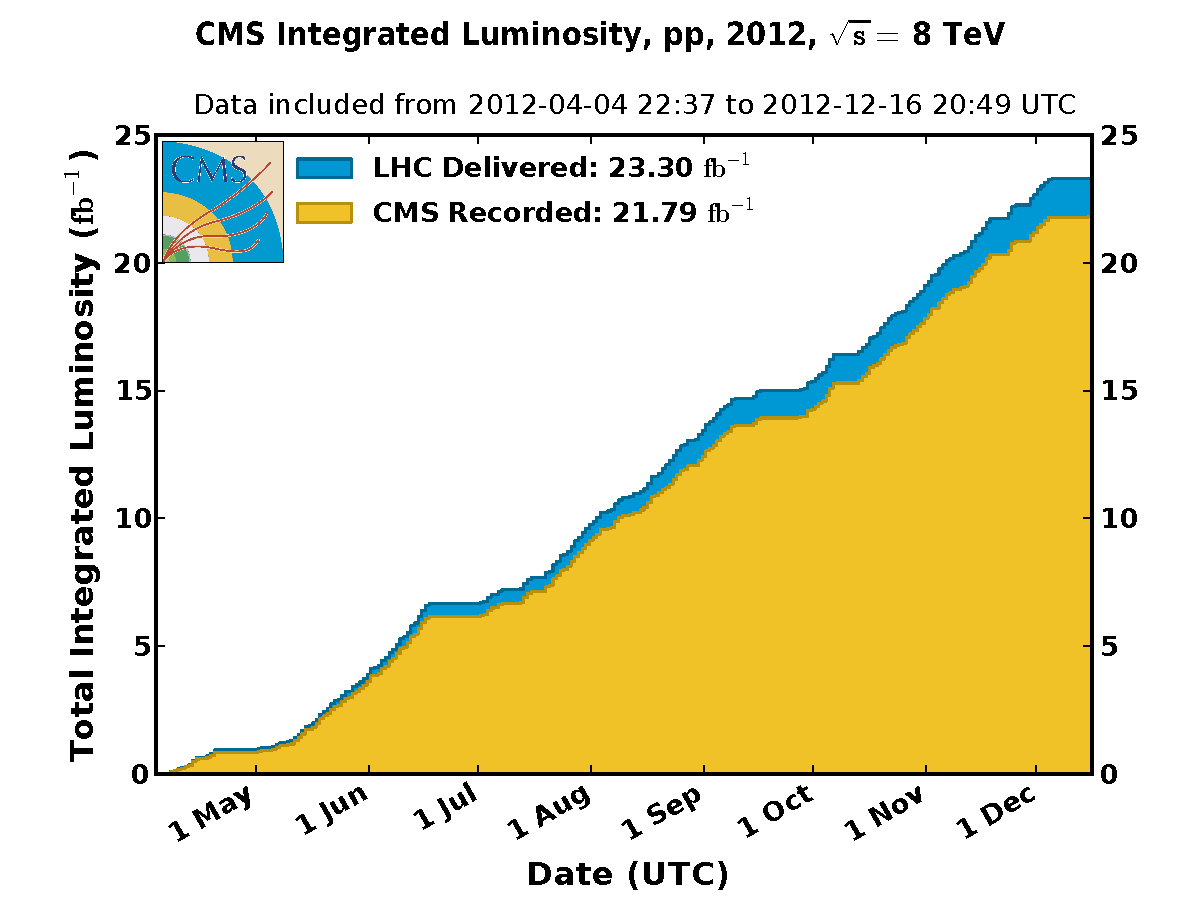
\includegraphics[width=0.8\textwidth]{lumi.pdf}
\caption[Summary of the amount of data delivered by the LHC and collected by CMS in 2012]
{\label{fig:cms_lumi}
The amount of data delivered by the LHC (red) and the amount of data
collected by the CMS detector (blue) as a function of date in the year 2012~\cite{lumitwiki}.
}
\end{center}
\end{figure}
% --------------------------------------------------------------------------- %

% --------------------------------------------------------------------------- %
% --------------------------------------------------------------------------- %
\section{Data Acquisition and Triggering}               \label {sec:cms_daq}
% --------------------------------------------------------------------------- %
% --------------------------------------------------------------------------- %
With nearly 80 million channels, and a bunch crossing every 25 ns having up to
40 proton-proton interactions per crossing, a huge amount of data is produced
by the CMS detector when the LHC is running at or near design luminosity.
At approximately 100 kilobytes of data per interaction, computing design
constraints limit the number of interactions that can be written to disk to
$\sim1000$ per second. The 25 ns between bunches give an interaction rate of 40
MHz resulting in a data reduction requirement of $\sim 10^5$. To accomplish
this, CMS has designed a data acquisition (DAQ) and trigger system which
utilizes a massive computing infrastructure and custom hardware. It is designed
to keep the most interesting interactions across a broad range of physics
goals. If a proton-proton interaction (an event), doesn't pass the trigger
system, it is lost forever.

Triggering occurs in two stages, the first of which is called Level
1 (L1) and has the task of reducing the load from 40 MHz down to 100
kHz~\cite{triggertdr1}. To do so, it employs a farm of custom electronics using
only coarse and lower resolution data to make decisions while storing the rest
of the event data in pipelines awaiting processing. Here, only calorimetric
and muon chamber information is available to make decisions based on the
energy and quantity of depositions in the detector. The data from the events
passing the L1 trigger are processed, compressed and zero-suppressed and sent
for handling by the DAQ. The DAQ then stores and processes the information and
sends it along to the second trigger phase. The High Level Trigger (HLT) is
a farm of standard CPUs running parallel that can run a more complete event
reconstruction to facilitate more informed decisions on whether to keep the
event. The object reconstruction algorithms used are simplified version of the
algorithms described in the following Section. A cartoon representation of the
trigger and DAQ chain can be seen in Figure~\ref{fig:cms_daq}. Between these
two trigger systems, the desired data reduction is achieved.

% --------------------------------------------------------------------------- %
\begin{figure}[tbhp]
\begin{center}
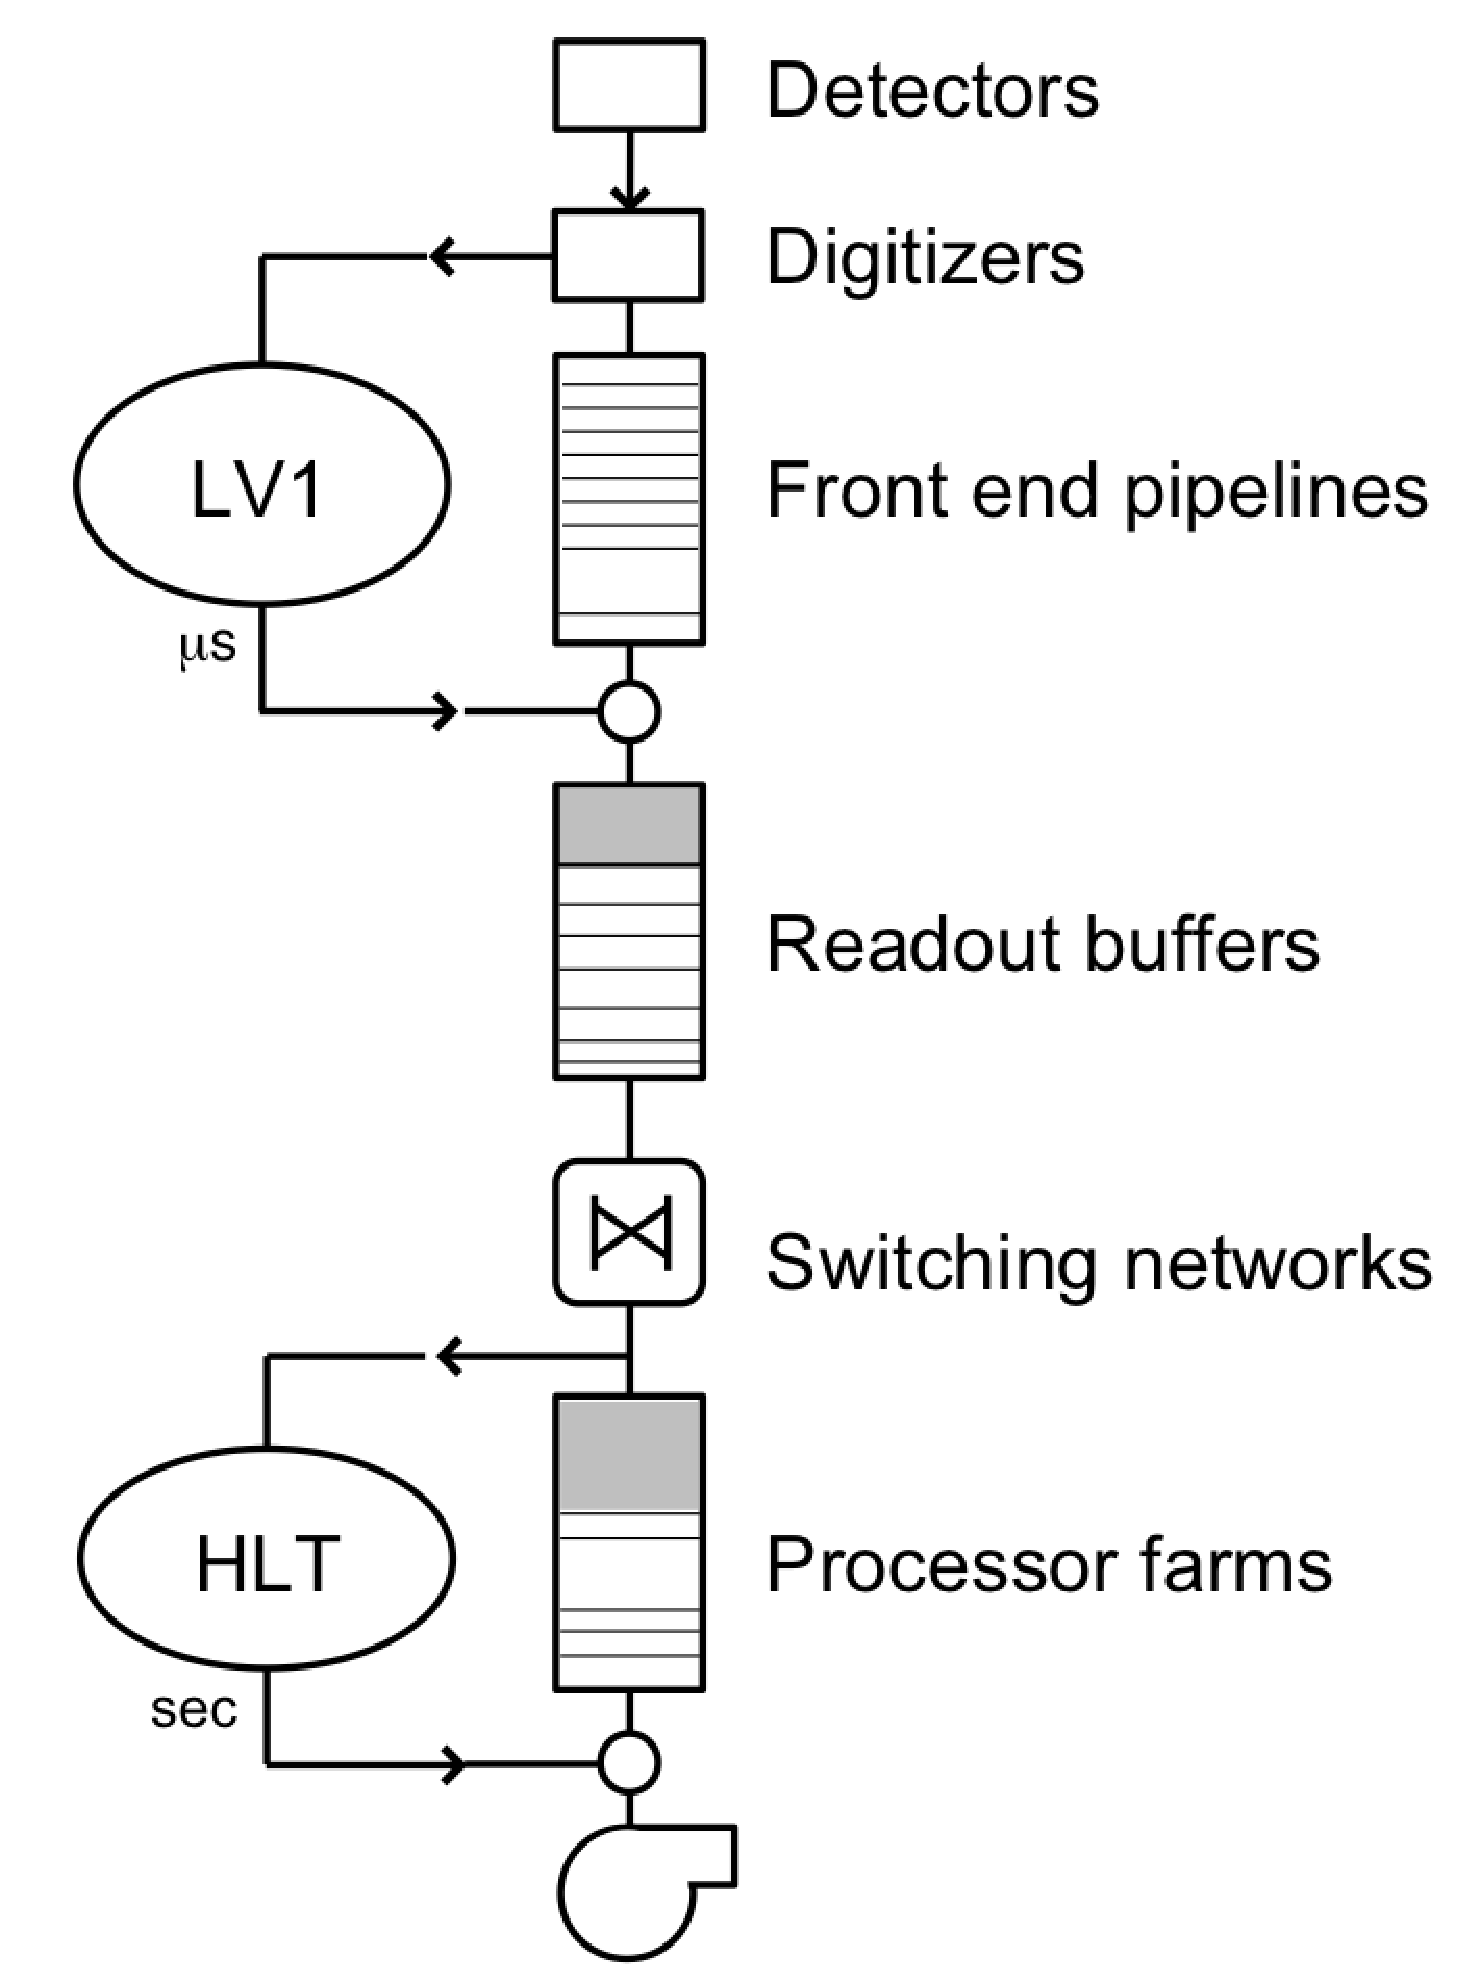
\includegraphics[width=0.4\textwidth]{daq_and_trig.pdf}
\caption{\label{fig:cms_daq}
Pictorial representation of the data acquisition system and
the flow of data from the CMS detector through both trigger levels~\cite{bourge}.
}
\end{center}
\end{figure}
% --------------------------------------------------------------------------- %

% --------------------------------------------------------------------------- %
% --------------------------------------------------------------------------- %
\section{Particle Reconstruction and Identification}
\label {sec:cms_reco}
% --------------------------------------------------------------------------- %
% --------------------------------------------------------------------------- %

The digitization of the events selected by the trigger only constitute
raw ingredients that need to be further processed in order to a give a
complete description of the particles present as the result of a proton-proton
collision. Many algorithms have been developed by the CMS collaboration to
reconstruct these particles; however, only the reconstruction algorithms used
in this thesis will be described here with a full description given in the
references. In this section we discuss charged particle, electron, muon, jet
and missing transverse energy reconstruction; which are the important objects
used in this analysis.

% --------------------------------------------------------------------------- %
% --------------------------------------------------------------------------- %
\subsection{Charged Particle Reconstruction}
\label {sec:cms_tracking}
% --------------------------------------------------------------------------- %
% --------------------------------------------------------------------------- %
Charged particles traversing the CMS detector first deposit energy in the
CMS tracker, leaving thousands of positional measurements to interpret
per bunch crossing. Determining the trajectory of these charged particles
amongst this collection of ``hits'' is an exercise in patter recognition.
Each charged particle can be described using five parameters that model
its trajectory as it is bent through the magnetic field. ``Tracking''
is the process of finding these ``tracks'' through the CMS tracking
system~\cite{pixel,mangano,trackingperformance}.

Individual silicon strip and pixel channels with a threshold above the
signal-to-noise ratio are clustered together based on proximity producing a
collection of positional measurements (along with the associated uncertainty).
These ``hits'' in the inner portion of the detector are used to seed multiple
tracking steps, each designed to find tracks from charged particles with
different properties. Each step takes an initial trajectory measurement
from the seed and propagates the trajectory from the inside to the outside
of the tracker using a combinatorial Kalman filter (CKF)~\cite{ckf}. After
propagation ends, the tracks are measured for quality and hits on high quality
tracks are removed from consideration before creating the seeds for the next
tracking step. The tracks produced with each step are then merged into a single
collection, eliminating duplicate tracks by comparing shared hits and keeping
tracks with higher quality.

The seeding step searches for combinations of two or three hits near the
beam line compatible with a particle trajectory with an energy above a given
threshold coming from the interaction point. The initial particle trajectory
is estimated using either a seed triplet or a seed pair and the beam spot.
There are seven tracking steps. The thresholds in each step is lowered
so that the initial steps have less background of seed candidates that lead
to tracks reconstructed for non-existent particles (fakes). The first two
steps are seeded using only triplets from the pixel detector, the second step
dropping the \pt threshold after the earlier higher \pt step. The third step
uses pairs of pixel hits to gain additional efficiency. The fourth step again
uses pixel triplets, but with a looser requirement on the compatibility with
the interaction point to search for displaced tracks and particles with longer
lifetimes. The fifth step again uses triplets, but allows for combinations
of hits in both the pixel and strip detectors. This allows for seeding of
particles which have slightly longer decay lengths or have a missed pixel hit
(due to detector inefficiency). The final two steps use pairs and triplets of
hits at further radii in the strip detector to search for particles which have
a large displacement.

In each step, after the seeds have been created, the initial trajectory
estimate is propagated inside-out, layer-by-layer through the detector using
the CKM algorithm. The algorithm accounts for losses of energy as the particle
traverse the material in the detector as well as the possibility of multiple
scatter. At each layer, the position of the trajectory is estimated and any
hits compatible with the position are added to the track. If more than one
compatible hit is found, multiple trajectories are kept and further propagated.
In addition, for each layer, a new trajectory is created assuming there is
no hit in the current layer to allow for detector inefficiency. The process
continues until either too many layers have been crossed without a hit or the
trajectory reaches the last layer of the tracker.

After the trajectories have been propagated, a final trajectory fit to the
collected hits is performed. Any outlying hits that fall too far from the
overall fit are removed. This gives a final accurate measurement of the tracks'
parameters. Vertex compatibility, number of hits in the track and the $\chi^2$
of the fit are used as quality control selections. Hits from tracks passing
tight quality selections are removed from consideration in subsequent tracking
steps.

After all seven steps have been performed, the resulting tracks from each step
are merged into a single collection. To ensure that no charged particles have
been reconstructed twice, any tracks that share a large fraction of its hists
are compared and only the best quality track is kept.

% --------------------------------------------------------------------------- %
% --------------------------------------------------------------------------- %
\subsection{Vertex Reconstruction}
\label {sec:cms_vertex}
% --------------------------------------------------------------------------- %
% --------------------------------------------------------------------------- %
In the high multiplicity environment of the LHC, it is essential to measure
the number of proton-proton interactions for each bunch crossing. Typically,
only one of the these interactions is responsible for the high \pt process
that triggered the event, and measuring the lepton impact parameters with
respect to the correct vertex is essential for the rejection of muons from
semi-leptonic flavor decays and electrons from photon conversions. Thus, a high
vertex reconstruction efficiency, a low fake vertex rate and the ability to
differentiate nearby interactions are all requirements needed for CMS's vertex
reconstruction.

Vertex reconstruction is performed in two steps. First, tracks are clustered
together using the deterministic annealing algorithm~\cite{davtx,dacms}. The
algorithm iteratively clusters tracks with nearby impact parameters first with
large windows and allowing a single track to be clustered multiple times.
Each iteration tightens the clustering window until a stopping condition is
met. Tracks are not allowed to cluster to vertices if their transverse impact
parameter is larger than 3 cm or the longitudinal impact parameter is larger
than 4 cm. The deterministic annealing algorithm was specifically choses due to
its high clustering efficiency even when faced with the noisy LHC environment.
Studies on the vertex efficiency show that the vertex reconstruction response
as a function of the number of interactions is linear.

The second step takes each cluster of tracks and fits the vertex position using
the adaptive vertex fitting algorithm \cite{vertexing,vtxfit}.  This algorithm
weighs tracks in the cluster based on compatibility with the vertex position
(and un-weights the tracks that are more incompatible) giving a good vertex
resolution of less than 50 \um depending on the number of tracks present in the
cluster.  More vertex reconstruction performance results can be found in
Reference~\cite{vtxtkres}.

% --------------------------------------------------------------------------- %
% --------------------------------------------------------------------------- %
\subsection{Electron Reconstruction}
\label {sec:cms_electron}
% --------------------------------------------------------------------------- %
% --------------------------------------------------------------------------- %

It is important to reconstruct and identify electrons efficiently and to
know their energy to a high precision. Electrons interact primarily via
the electromagnetic force and hence deposit a majority of their energy
in the ECAL. However, due to the large amount of material the electron
must traverse in the silicon tracker, the electron radiates a significant
amount of energy via bremsstrahlung and hence the ``footprint'' of the
electron's energy distribution is very complex. In addition, other particles
also leave a significant amount of energy in the ECAL, namely hadrons,
in particular the $\pi^0$, which decays predominantly to two photons .
Therefore, strong rejection of reconstructed electrons originating from
sources other than true electrons from the hard interaction (fakes) is needed
in the form of electron identification. The identification of electrons and
rejection of fake electrons are left to be presented in the context of this
analysis in Section~\ref{sec:evtsel_el} while the reconstruction algorithm is
summarized below. More information about electron reconstruction can be found
in References~\cite{baffiReco,egmReco,egm2013}.

The first step of electron reconstruction is to identify clusters of energy in
the ECAL, i.e. areas where many crystals in close proximity have large energy
deposits. As the electron travels through the silicon tracker, bremsstrahlung
causes losses of energy through radiated photons which then also deposit
energy in the ECAL. The strong magnetic field bends the electron in the
azimuthal direction and it will radiate energy, in the form of photons, which
will spread energy along $\phi$ in the ECAL. Therefore the footprint
of the electron is such that it is long in $\phi$ and narrow in $\eta$ and
multiple deposits of energy need to be clustered together to form a ``Super
Cluster (SC)'' containing the full amount of energy originally possessed by the
electron.

After all SCs have been assembled, electron reconstruction continues by
searching for the footprint of the electron in the tracker. Hits in the pixel
detector compatible with the energy-weighted center of the SC are
identified allowing for both positive and negative charge hypotheses. If two
or three compatible pixel hits are discovered, they are used to seed a track
building algorithm similar to that described in Section~\ref{sec:cms_tracking}.
The sole difference in the case of electrons is that track fitting is done with
a Gaussian sum filter (GSF)~\cite{gsf} algorithm which can handle the large
changes in electron trajectory due to bremsstrahlung.

In addition to this approach seeded by SCs, a separate algorithm is run in
parallel. This is a ``particle-flow'' based approach which will be described
in full in Section~\ref{sec:cms_pf}. Instead of first building a SC, the
algorithm searches for pixels seeds for all clustered energy. For each found
seed, the algorithm completes the trajectory building and then searches for
clusters to add to the electron. At each layer in the tracker along the
electron track, the position in the ECAL pointed to by the electron's current
momentum is used to search for additional compatible clusters that originate
from a radiated photon. After both algorithms are complete, the two collections
of electrons are merged. The SC seeded algorithm dominates at higher energies
($>20 \GeV$) while the track-seeded algorithm adds significant efficiency at
lower energies as well as in crowded environments such as near or inside a jet.
A graphic showing the different pieces of the two algorithms can be seen in
Figure~\ref{fig:cms_elereco}.

% --------------------------------------------------------------------------- %
\begin{figure}[tbhp]
\begin{center}
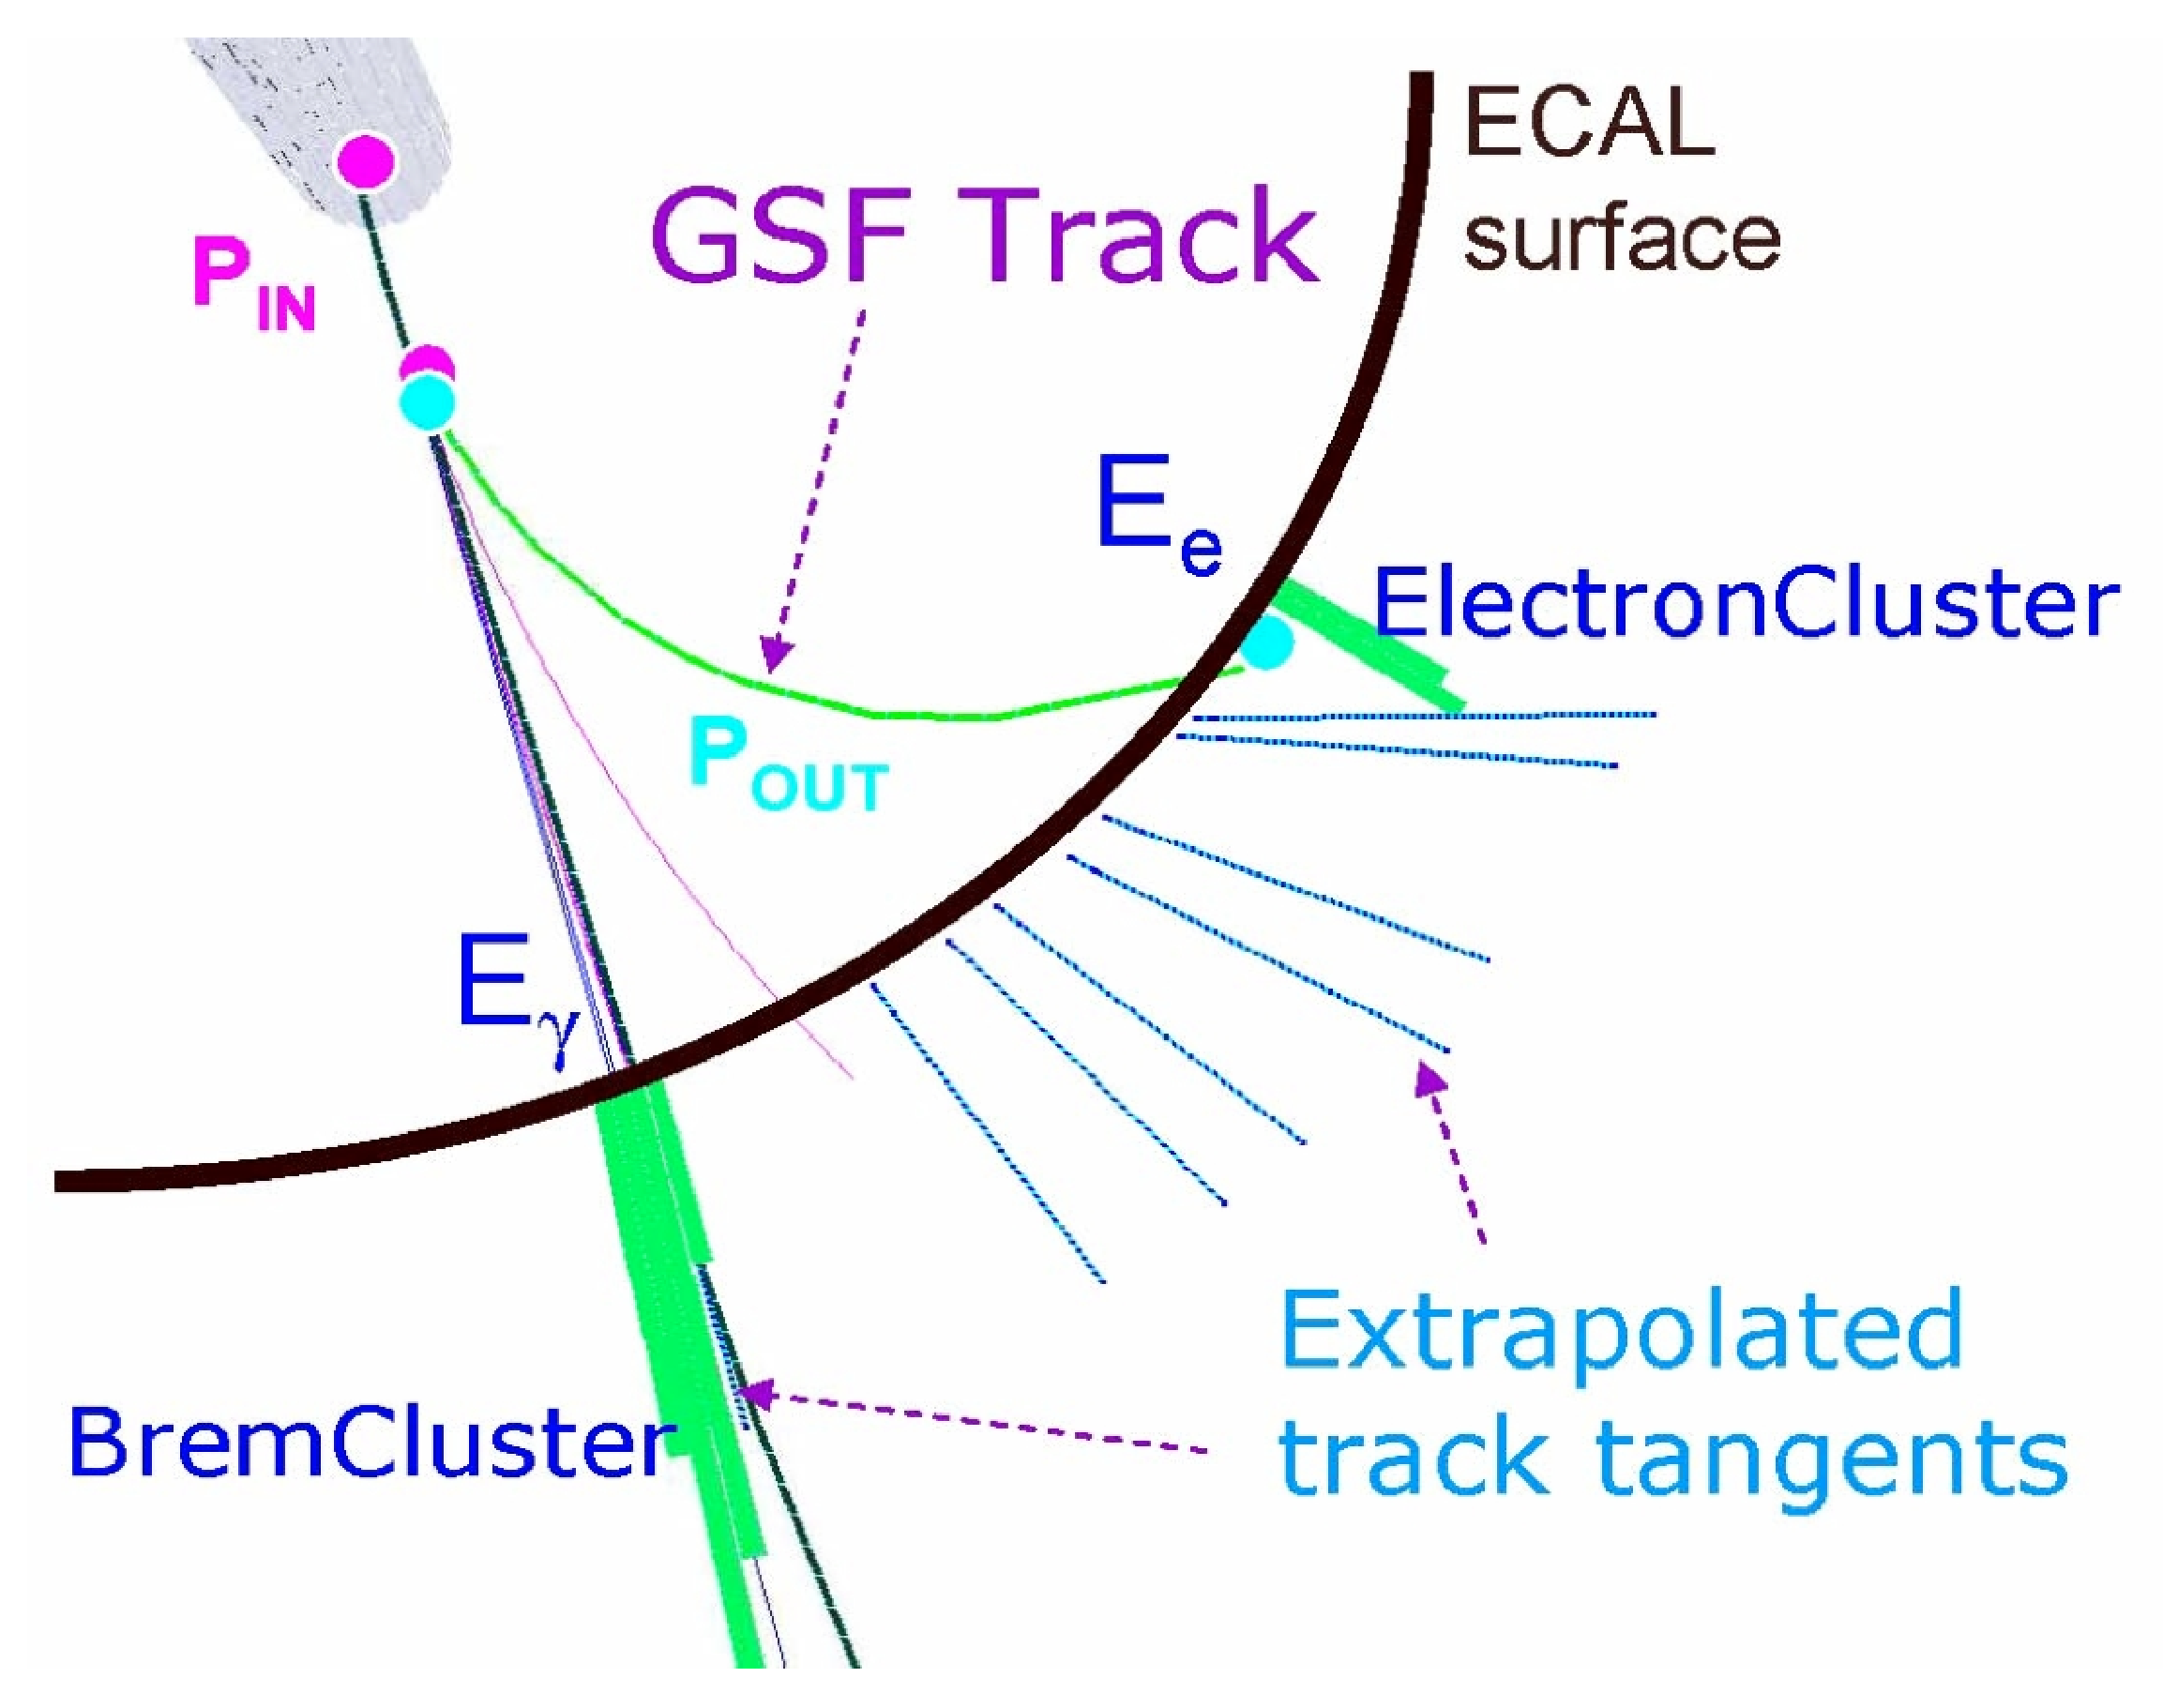
\includegraphics[width=0.6\textwidth]{elereco.pdf}
\caption[Depiction of the different portions of the electron reconstruction algorithm]
{\label{fig:cms_elereco}
Depiction of the different portions of the electron reconstruction algorithm.
Here the electron radiated a photon with a significant amount of energy early
in its traversal of the tracker and therefore there are two large clusters
(depicted in green) of energy present in the ECAL (depicted in black)~\cite{bourge}.
}
\end{center}
\end{figure}
% --------------------------------------------------------------------------- %

% --------------------------------------------------------------------------- %
% --------------------------------------------------------------------------- %
\subsection{Muon Reconstruction}
\label {sec:cms_muon}
% --------------------------------------------------------------------------- %
% --------------------------------------------------------------------------- %
Muons, in contrast to electrons, penetrate through to the outer regions of
the CMS detector due to their much higher mass and hence have a smaller
background contamination. Objects mis-reconstructed as muons in this
analysis come mostly from high energy hadrons which ``punch-through'' the
dense calorimeters and leave deposits in the muon detector. Another source
of background muons come from semi-leptonic decays of pions and kaons to
real muons. Reconstruction efficiency for muons is quite high and we can
therefore apply tight identification requirements to reduce these backgrounds
for this analysis. This is discussed in Section~\ref{sec:evtsel_mu}. The muon
reconstruction algorithm is discussed below, with more detailed information
available in References~\cite{muontdr,muonReco}.

Muon reconstruction begins by building segments in the muon sub-detector.
Positions of hits in the DT and CSCs are matched together to form small
segments compatible with a single particle passing through each chamber. Using
these segments (as well as hits in the RPCs) as positional measurements,
tracking is performed starting from the inside of the muon chamber and working
out to the outer edge of the muon system. Here, the Kalman Filter is used
to propagate and fit the muon tracks accounting for the loss of energy and
multiple scattering as the muon passes through the iron yoke. These tracks
built in the muon system are called ``Stand-Alone'' muons (SAM).

Since muons first passed through the CMS tracker, the SAMs are used to look
for tracks built in the silicon tracker matching the expected trajectory and
energy. Matched tracks are combined with the muon-only tracks and a global
refit is performed (again with the Kalman Filter algorithm). The resulting
muons are called ``global muons.''

In addition, another muon reconstruction algorithm is used to build muons
with information from the both the tracker and the muon system. ``Tracker''
muons are seeded from the tracks built in the silicon tracker. Each track is
extrapolated through both the ECAL and HCAL taking into account the expected
trajectory and uncertainty based on the magnetic field and the amount of
material it traverses. The energy deposited in the ECAL and HCAL at the expected
position of the muon's trajectory is checked to ensure compatibility with the
expectation from the minimum ionizing particle. The expected muon trajectory
is then extended into the muon system checking for matching segments. This
algorithm gives higher efficiency for lower \pt muons at the expense of a
larger background; however, muon identification selections can be applied for
further suppression.

% --------------------------------------------------------------------------- %
% --------------------------------------------------------------------------- %
\subsection{Particle Flow Reconstruction}
\label {sec:cms_pf}
% --------------------------------------------------------------------------- %
% --------------------------------------------------------------------------- %
The algorithms discussed up to this point have been the so-called
``detector-based'' algorithms. That is, reconstruction in each of the local
sub-detectors drives the higher level reconstruction of particles that leave their
signature in the respective sub-detectors. The ``particle-flow'' (PF) algorithm
is a paradigm shift from this type of algorithm in that it uses the very fine
segmentation of the CMS detector to search for an individual particle across
all the sub-detectors. For example, a charged hadron will leave a track in the
silicon tracker, a small amount of energy in the ECAL and will be deposited in
the HCAL, dissipating most of its energy. PF is used to identify particles in
this manner. When complete, the algorithm aims to have produced a list of all
the particles produced during the collision.

One large disadvantage of detector-based methods is the fact that energy
could be double counted, while with the PF algorithm, a global reconstruction
of the event is done on a particle-by-particle basis ensuring that double
counted energy is minimized. The resulting list of particles produced
by this algorithm is used extensively across many analyses at CMS. The
calculation of missing transverse energy (\met), jet reconstruction, and $\tau$
reconstruction are among the most important. The following briefly describes
the particle flow algorithm; however, a complete description can be found in
References~\cite{pfReco,pfComm}.

Before the PF reconstruction begins, local reconstruction in each of the
sub-detectors is completed and provides tracks from the silicon detector
(Section~\ref{sec:cms_tracking}), clustered energy in both the ECAL and HCAL
(similar to those discussed in Section~\ref{sec:cms_electron}) and the local
reconstruction product in the muon system (Section~\ref{sec:cms_muon}). The
general strategy is then to ``link'' these different inputs together to form
the complete picture of particles traversing through the detector. Objects
from each of the sub-detectors in close proximity are first grouped together
in blocks. Each block usually contains a few different inputs from each of the
detectors, i.e. a track pointing to an ECAL cluster, or an ECAL and HCAL energy
cluster adjacent to each other. Any blocks linked to signatures from isolated
muons or electrons are removed, as these have a very clean signature with very
little background. The blocks belonging to these particles (including the
clusters from radiated products as discussed in Section~\ref{sec:cms_electron})
are then removed from the list of unidentified blocks and added the list of PF
muons and electrons. Next, the momentum of any track pointing to calorimetric
clusters is compared to the energy contained in the ECAL or HCAL clusters.
If the energy and momentum of the two are compatible, the object is labeled
as a charged hadron, its energy is estimated as a weighted sum from both
objects, and its constituents are removed from the list and added to the list
of PF charged hadrons. If there is significantly more energy in the track
than is deposited in the calorimeter, a secondary muon identification is
performed searching for non-isolated lower \pt muons. If identified, again,
these constituents are removed and added to the PF muon list. If no muon is
found, tighter track requirements are applied to reject mis-reconstructed
tracks. If there is significantly more energy in the calorimeters, neutral
hadrons and photons are created comprising the energy unaccounted for by the
track. At this point, only unlinked clusters remain and all ECAL clusters are
hypothesized to be photons with all HCAL clusters hypothesized to be neutral
hadrons and added to their respective lists.

% --------------------------------------------------------------------------- %
% --------------------------------------------------------------------------- %
\subsection{Calculation of Missing Transverse Energy}
\label {sec:cms_met}
% --------------------------------------------------------------------------- %
% --------------------------------------------------------------------------- %
Neutrinos and other non-interacting particles from BSM theories, such
as neutralinos from supersymmetry, leave no signature as they traverse
the detector. Yet, we can infer their existence, transverse direction and
energy by looking at the sum of all of the transverse energy in the event.
As the two protons collide, all of their momentum is in the $z$-direction
(and negative-$z$), with no momentum transverse to the beam line. Momentum
conservation then requires that the transverse vectorial sum of all energy in
the event should sum to zero. If this calculation is performed and an imbalance
(missing transverse energy, \met) is detected, a non-interacting particle is
hypothesized to have escaped from the detector.

The \met reconstruction algorithm used by this analysis takes as input the full
collection of particle flow candidates and produces the negative vectorial sum.
Particle flow \met is defined as
\[
{\bf\met} =  - \displaystyle\sum_{i} {\bf \pt}^{i},
\]
where the summation is over all particles reconstructed with the particle
flow algorithm described in the previous section. Further information about
\met may be found in Reference \cite{metPerformance}.

% --------------------------------------------------------------------------- %
% --------------------------------------------------------------------------- %
\subsection{Jet Reconstruction}
\label {sec:cms_jets}
% --------------------------------------------------------------------------- %
% --------------------------------------------------------------------------- %
Jets are the experimental signatures of quarks and gluons produced in
high-energy processes such as proton-proton collisions. As quarks
and gluons have a net color charge and cannot exist freely due to
color-confinement, they are not directly observed in Nature. Instead, they
come together to form color-neutral hadrons, a process called hadronization
that leads to a collimated spray of hadrons called a jet.

Jet reconstruction is done by clustering nearby reconstructed PF
candidates. Starting with the highest \pt candidates as seeds, clustering is
done using the anti-$k_T$ algorithm~\cite{antikt} with a distance parameter of
$\DR=0.5$, defined in the $\eta-\phi$ plan. This clustering algorithm
uses a distance measurement inversely proportional to the square of each
particle's \pt and thus gives stability in the cases of infrared or collinear
radiation.

The use of PF candidates gives good jet energy response due to the high
reconstruction efficiencies of charged hadrons and photons which make up about
90\% of the jet's energy. However, some corrections are still applied to 
the jet energy with these energy scale corrections factorized into three steps.
First, an offset correction is applied to reduce the energy of the jet based on
the amount of pile-up in the event. A pile-up density is calculated using the
FastJet method~\cite{fastjet} to compute mean energy of jets in the event and
the ghost particle method for calculating jet areas~\cite{jetarea}.

Next, corrections for the detector response are made as a function of jet
\pt and $\eta$. The first portion of this correction is applied based on
measurements of simulated jet energies. The last correction is made to account
for the differences in the true CMS response between the physical and simulated
detector. The differences are measured by looking at jet energies in di-jet,
\gj and \Zj events where the object recoiling against the jet can be used to
measure the true jet energy. The uncertainty on this method is less that 5\%,
smaller than the overall jet energy resolution which ranges from 8\% to 15\%,
depending on the jet \pt and $\eta$. The remaining differences are explicitly
corrected for in data in the residual correction step, which completes the
jet energy correction chain. A full picture of jet reconstruction and energy
corrections can be found in Reference~\cite{cmsjetcal}.

% --------------------------------------------------------------------------- %
% --------------------------------------------------------------------------- %
\subsection{b-Jet Identification}                       \label {sec:cms_btags}
% --------------------------------------------------------------------------- %
% --------------------------------------------------------------------------- %

The identification of b-jets will be a major handle to select possible signal
event. One of the design requirements of the tracker was to find displaced
vertices of the long lived hadrons produced by b-quarks. Many algorithms were
designed to identify displaced vertices present in b flavored jets (b-jets);
however, we only discuss the one algorithm that is used in this analysis, the
Combined Secondary Vertex method (CSV)~\cite{btagging}.

The presence of a secondary vertex and the kinematic variables associated with
this vertex can be used to discriminate between a b and non-b jet. Two of these
variables are the distance and direction between the primary and secondary
vertices (the flight distance and direction). The significance of the flight
distance (the ratio of the flight distance to its estimated uncertainty) can be
used as a discriminating variable. In the CSV algorithm, the flight distance
information is combined with track-based lifetime information. By using this
additional information, the algorithm provides discrimination also in cases
where no secondary vertices are found, increasing the efficiency with respect
to using the secondary vertex information alone. The vertex category is defined
as
\begin{itemize}
  \item real: There exists a secondary vertex.
  \item pseudo: When no real vertex is found, tracks with a high impact parameter
significance ($S_{IP}$, the impact parameter divided by its uncertainty) are used
to create a ``pseudo'' vertex.
  \item no vertex: When no real or pseudo vertex is found.
\end{itemize}
In addition to the vertex category, the following variables are used to form a
discriminating variable (in the ``no vertex'' category, only the last two are
used):
\begin{itemize}
  \item the flight distance significance in the transverse plane (``2D'');
  \item the vertex mass;
  \item the number of tracks at the vertex;
  \item the ratio of the energy carried by the tracks at the vertex with respect to all tracks in the jet;
  \item the \pr of the tracks at the vertex with respect to the jet axis;
  \item the 2D $S_{IP}$ of the first track that raises the invariant mass above the charm threshold of 1.5\GeVcc;
  \item the number of tracks in the jet;
  \item the 3D $S_{IP}$ for each track in the jet.
\end{itemize}
A likelihood ratio is built from these variables. It is used to discriminate
between b and c jets and between b and light-parton jets. The distribution
of the CSV discriminator is shown in Figure~\ref{fig:cms_btag_disc}. In
this analysis, we use the ``medium'' working point, which is any jet with a
discriminator value greater than 0.679 is ``tagged'' as a b-jet.
% --------------------------------------------------------------------------- %
\begin{figure}[!hbt]
\begin{center}
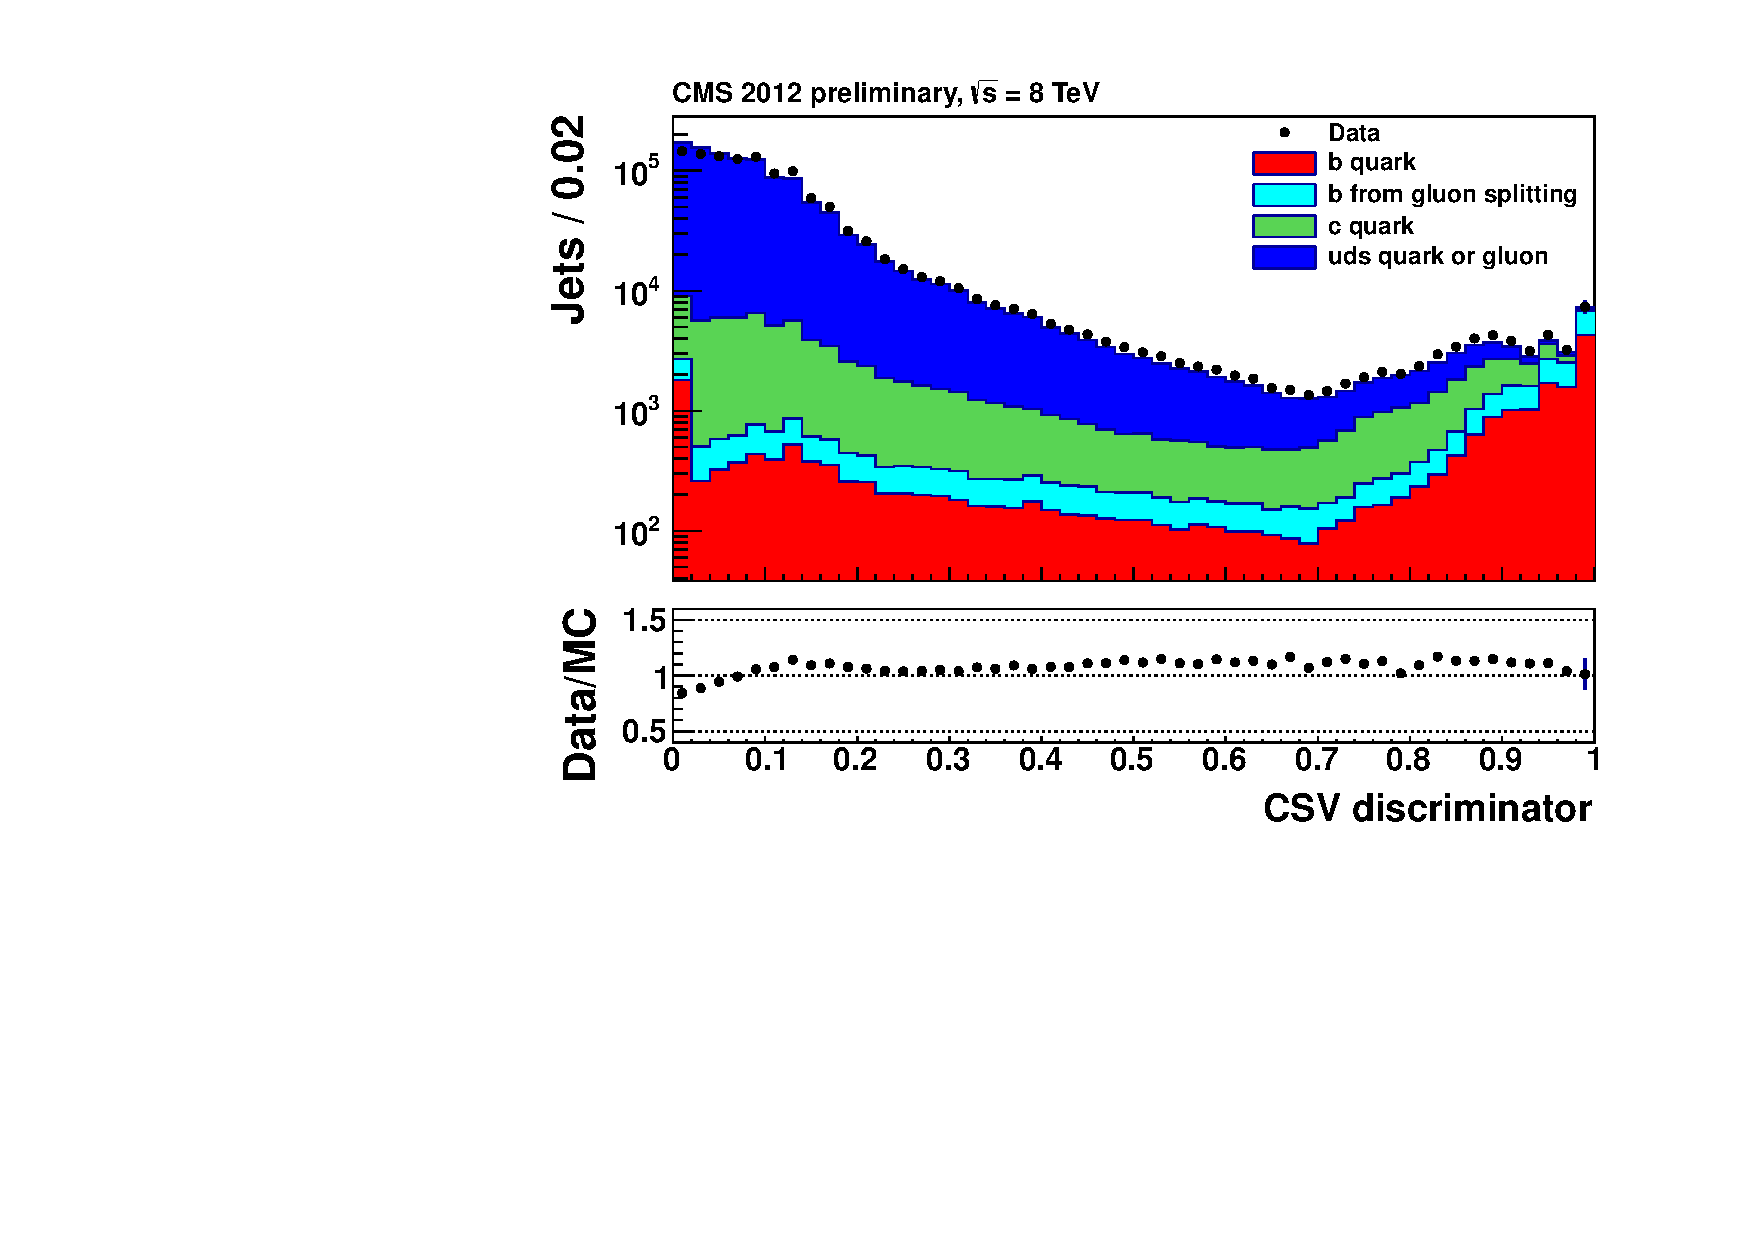
\includegraphics[width=0.7\textwidth]{btag_disc.pdf}
\caption[Combined Secondary Vertex algorithm discriminant for data and simulation.]
{\label{fig:cms_btag_disc}
Combined Secondary Vertex algorithm  discriminant for
data (black points) and compared to simulation of lighter flavor jets (green
and blue) as well as b-jets (cyan and red).  Larger values of the discriminant
are more indicative of heavy flavor jets.  The ratio between data and simulation
is shown at bottom~\cite{btagging}.
}
\end{center}
\end{figure} 
% --------------------------------------------------------------------------- %

% --------------------------------------------------------------------------- %
% \begin{figure}[!hbt]
% \begin{center}
% 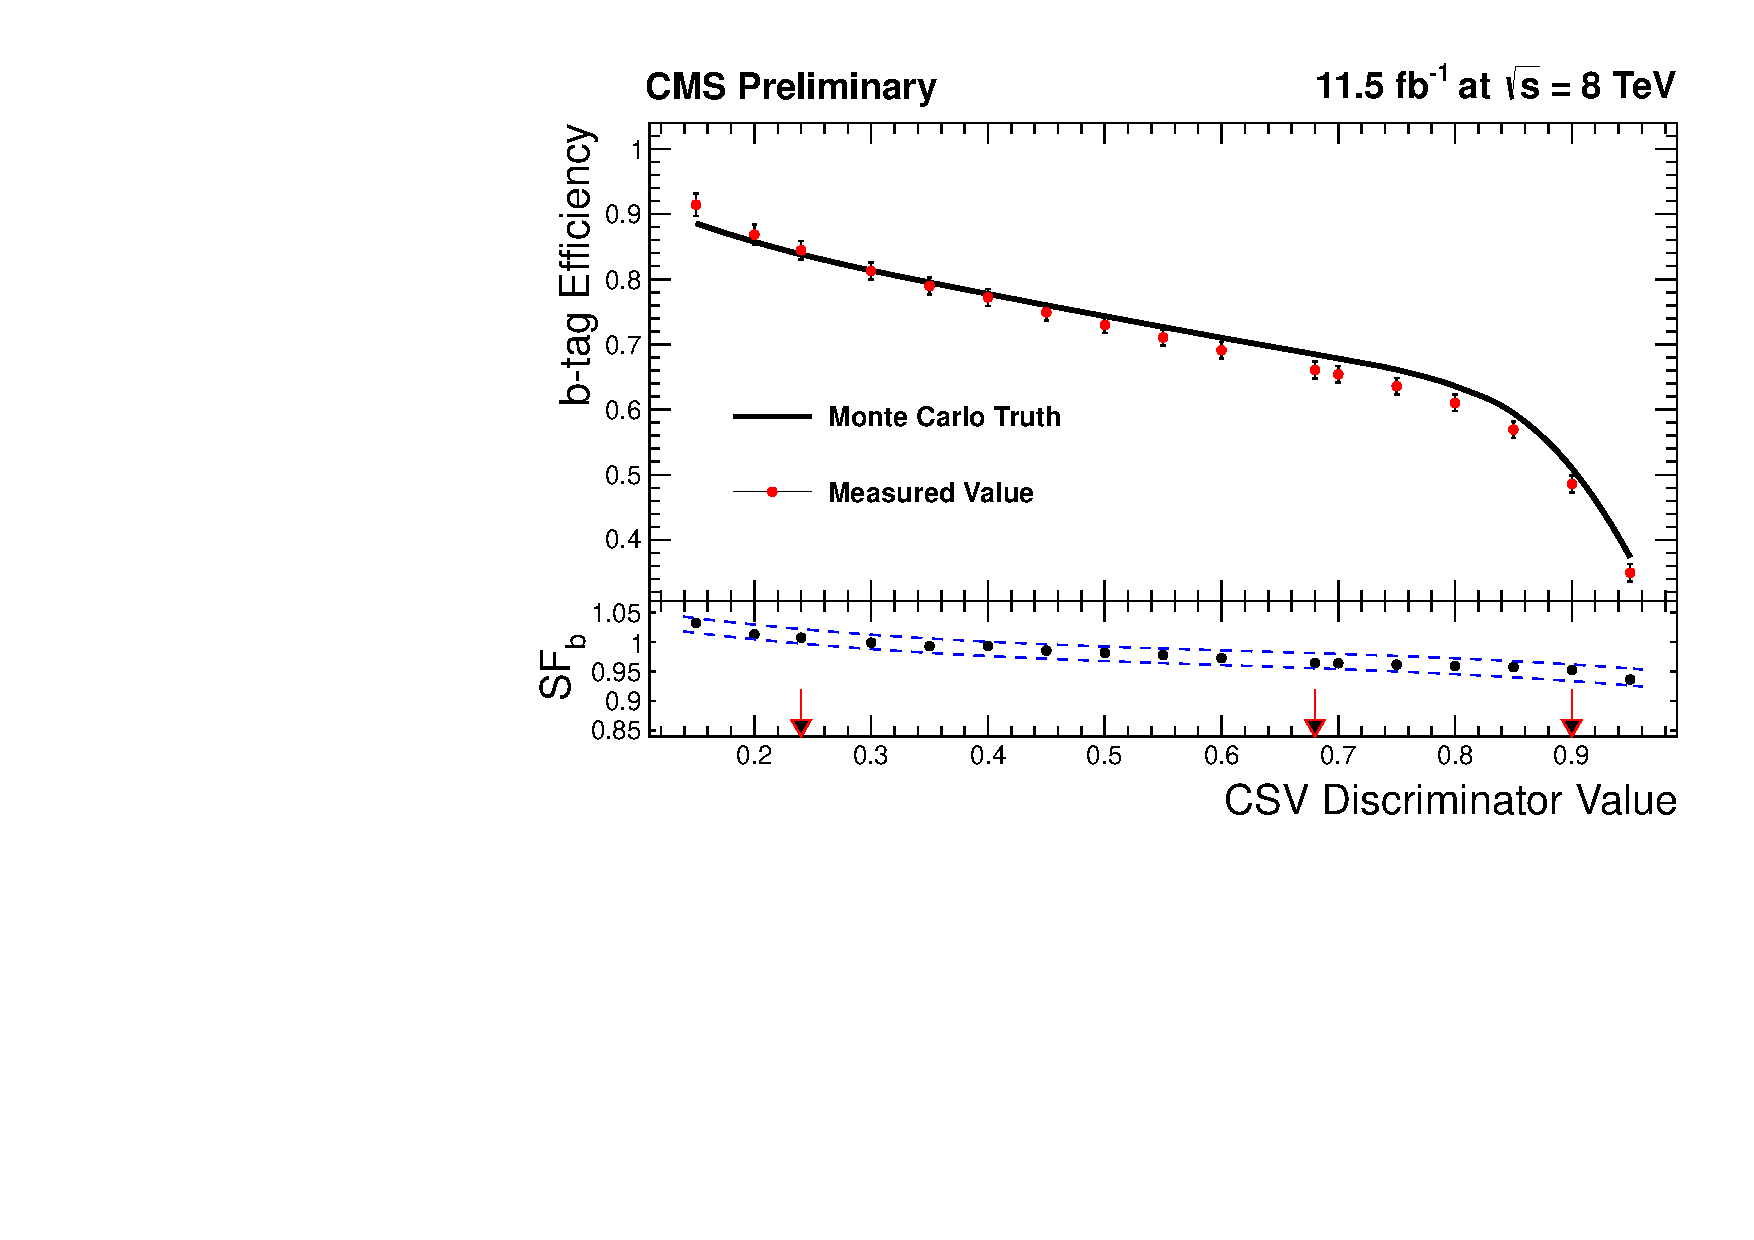
\includegraphics[width=0.7\textwidth]{btag_eff.pdf}
% \caption[b-jet efficiency for the track counting high effeciency b-tagging algorithm.]
% {\label{fig:cms_btag_eff}
% b-jet efficiency for the CSV algorithm in data (red points) and simulation
% (black line) as a function of the track counting high efficiency algorithm
% output discriminant. The ratio of data to simulation is plotted below with the
% blue band indicating the uncertainty on the measurement~\cite{btagging}.
% }
% \end{center}
% \end{figure} 
% --------------------------------------------------------------------------- %


% --------------------------------------------------------------------------- %
% --------------------------------------------------------------------------- %
\chapter{Same-Sign Dilepton Signature}
\label {ch:ss}

As discussed in Section~\ref{sec:intro_ss}, there are many models that predict
same-sign dileptons, hadronic jets, and \met. In order to determine if there is
an excess of events, an accurate prediction of the expected background to this
signature must be performed. In this chapter, a brief description will be given
for the SM background processes that give genuine same-sign dileptons that are
both prompt and isolated (rare SM). These constitute an irreducible background
to the analysis that must be accounted for. These processes are discussed in
Section~\ref{sec:ss_rare}.

The other two major sources of background include objects mis-identified as
selected leptons (fakes) and leptons with a mis-identified charge and from
genuine opposite-sign pairs (charge flips). These backgrounds sources are a
result of the failure of the selection to properly classify these events and
these sources are discussed in Section~\ref{sec:ss_bkgd}.

% --------------------------------------------------------------------------- %
% --------------------------------------------------------------------------- %
\section{Rare Standard Model Processes}
\label{sec:ss_rare}
% --------------------------------------------------------------------------- %
% --------------------------------------------------------------------------- %

As discussed previously, the main source of irreducible background is processes
that produced genuine prompt and isolated same-sign leptons in the final state.
In this section, we provide a brief description of the main processes that the
SM predicts and are included in this analysis.

% --------------------------------------------------------------------------- %
\subsection{Top Processes}
\label{sec:ss_rare_top}
% --------------------------------------------------------------------------- %

Processes involving top production with an associated gauge boson is are a
significant source of same-sign dileptons. This can be seen by the example Feynman
diagram shown in Figure \ref{fig:feyn_ttw}.
% --------------------------------------------------------------------------- %
\begin{figure}[!htb]
\begin{center}
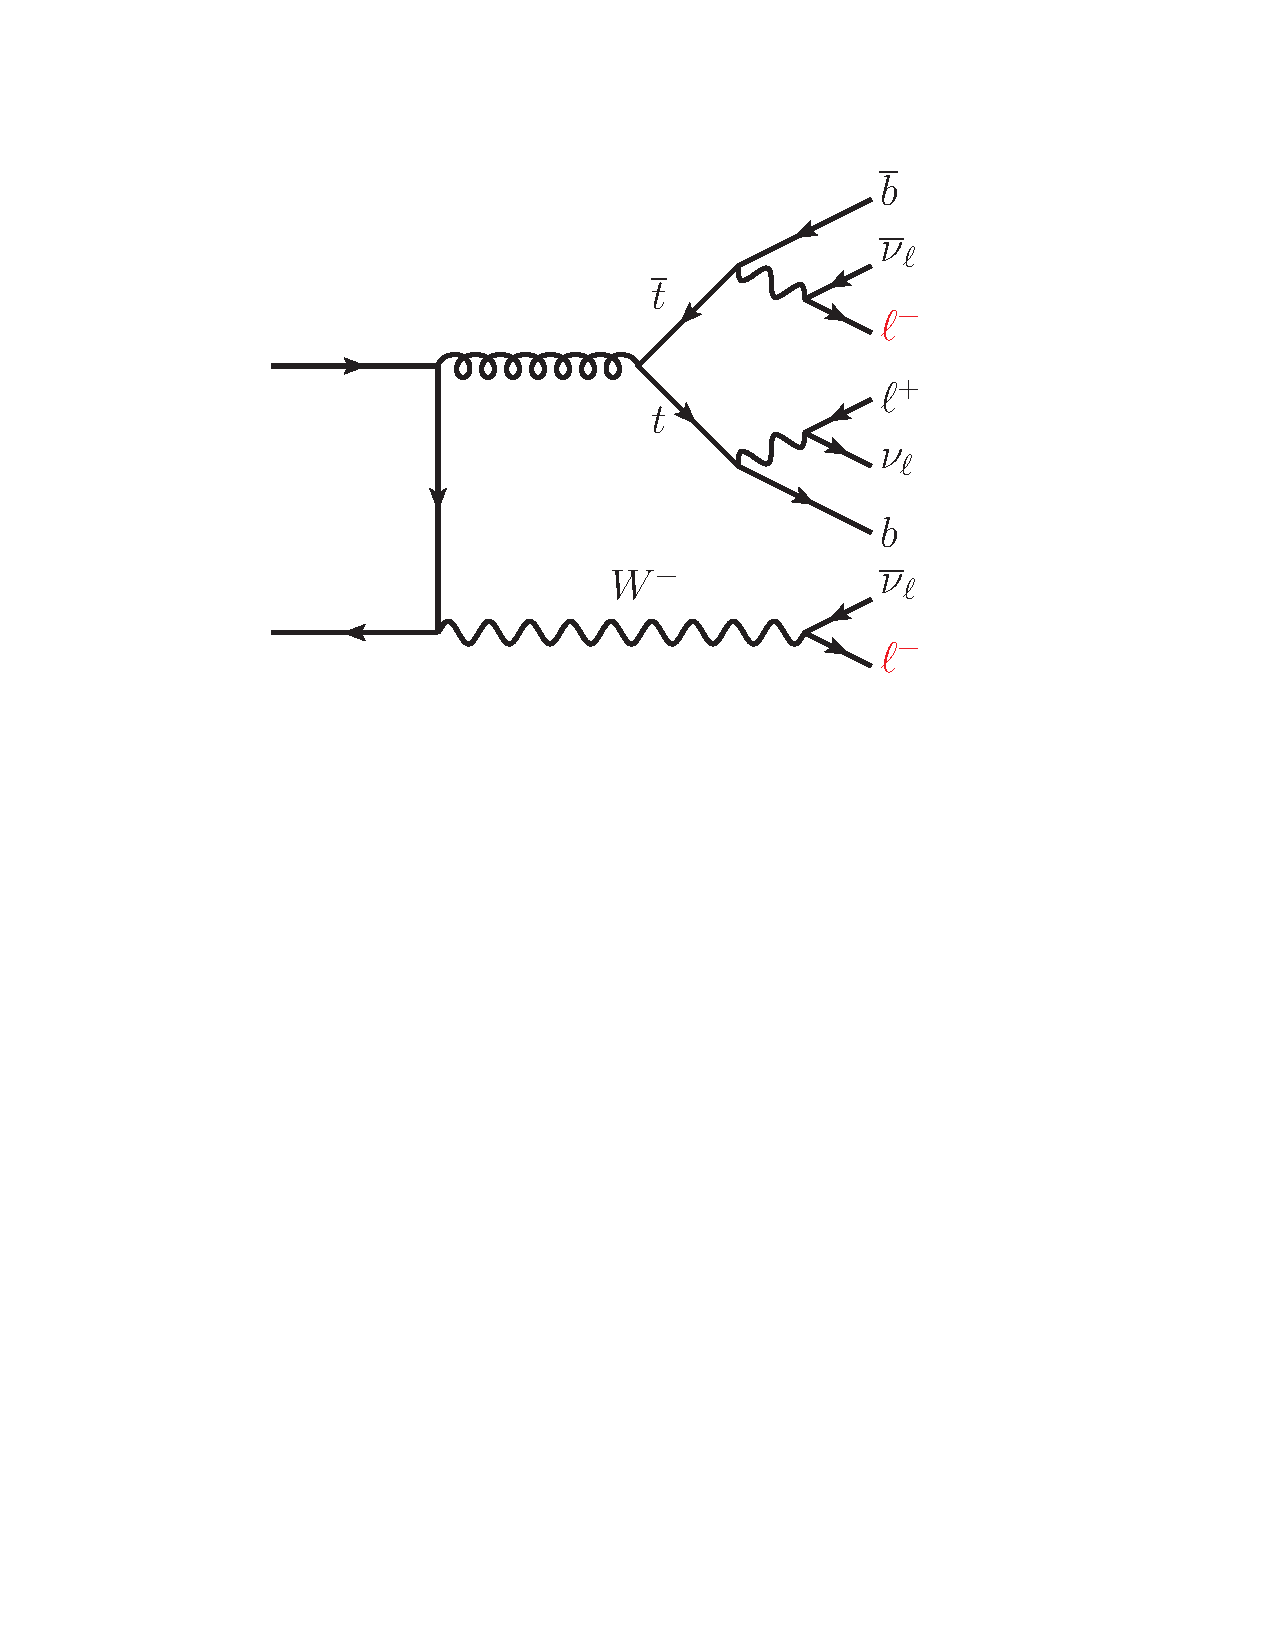
\includegraphics[width=0.8\textwidth, clip = true, trim = 1in 6.5in 1in 1in]{ttw.pdf}
\caption[Feynman diagram for \ttW]
{\label{fig:feyn_ttw}
Example leading order Feynman diagram for $pp \to \ttW \to 3\ell\nu + X$.
}
\end{center}
\end{figure}
% --------------------------------------------------------------------------- %
Top processes that are considered in this analysis are listed below:
\begin{itemize}
\item \ttW: The \W decays leptonically and the top quark with the same charge as the \W also decays leptonically ($t \to \ell^{\pm}\nu b$ and $W^{\pm} \to \ell^{\pm}\nu$).
\item \ttZ: The \Z decays leptonically and at least one of the top quarks also decays leptonically ($t \to \ell^{\pm}\nu b$ and \Zlplm).
\item \ttG: The $\gamma$ decays leptonically and at least one of the top quarks also decays leptonically ($t \to \ell^{\pm}\nu b$ and \Glplm).
\item \tbZ: The \Z decays leptonically and the top quarks also decays leptonically ($t\bar{b} \to \ell^-\nu \bar{b}$ and \Zlplm).
\item \ttWW: At least one of the \W's decay leptonically and one of the top quarks with the same sign also decays leptonically ($t \to \ell^{\pm}\nu b$ and $W^{\pm} \to \ell^{\pm}\nu$).
\end{itemize}

% --------------------------------------------------------------------------- %
\subsection{Two Gauge Boson Processes}
\label{sec:ss_rare_diboson}
% --------------------------------------------------------------------------- %
 
Processes involving the production of two electroweak bosons in the same event
can easily produce same-sign leptons. What makes them rare is their actual
production is quite low due to the mass of these bosons. A typical
example can be seen from the Feynman diagram shown in Figure~\ref{fig:feyn_wz}
below:
% --------------------------------------------------------------------------- %
\begin{figure}[!htb]
\begin{center}
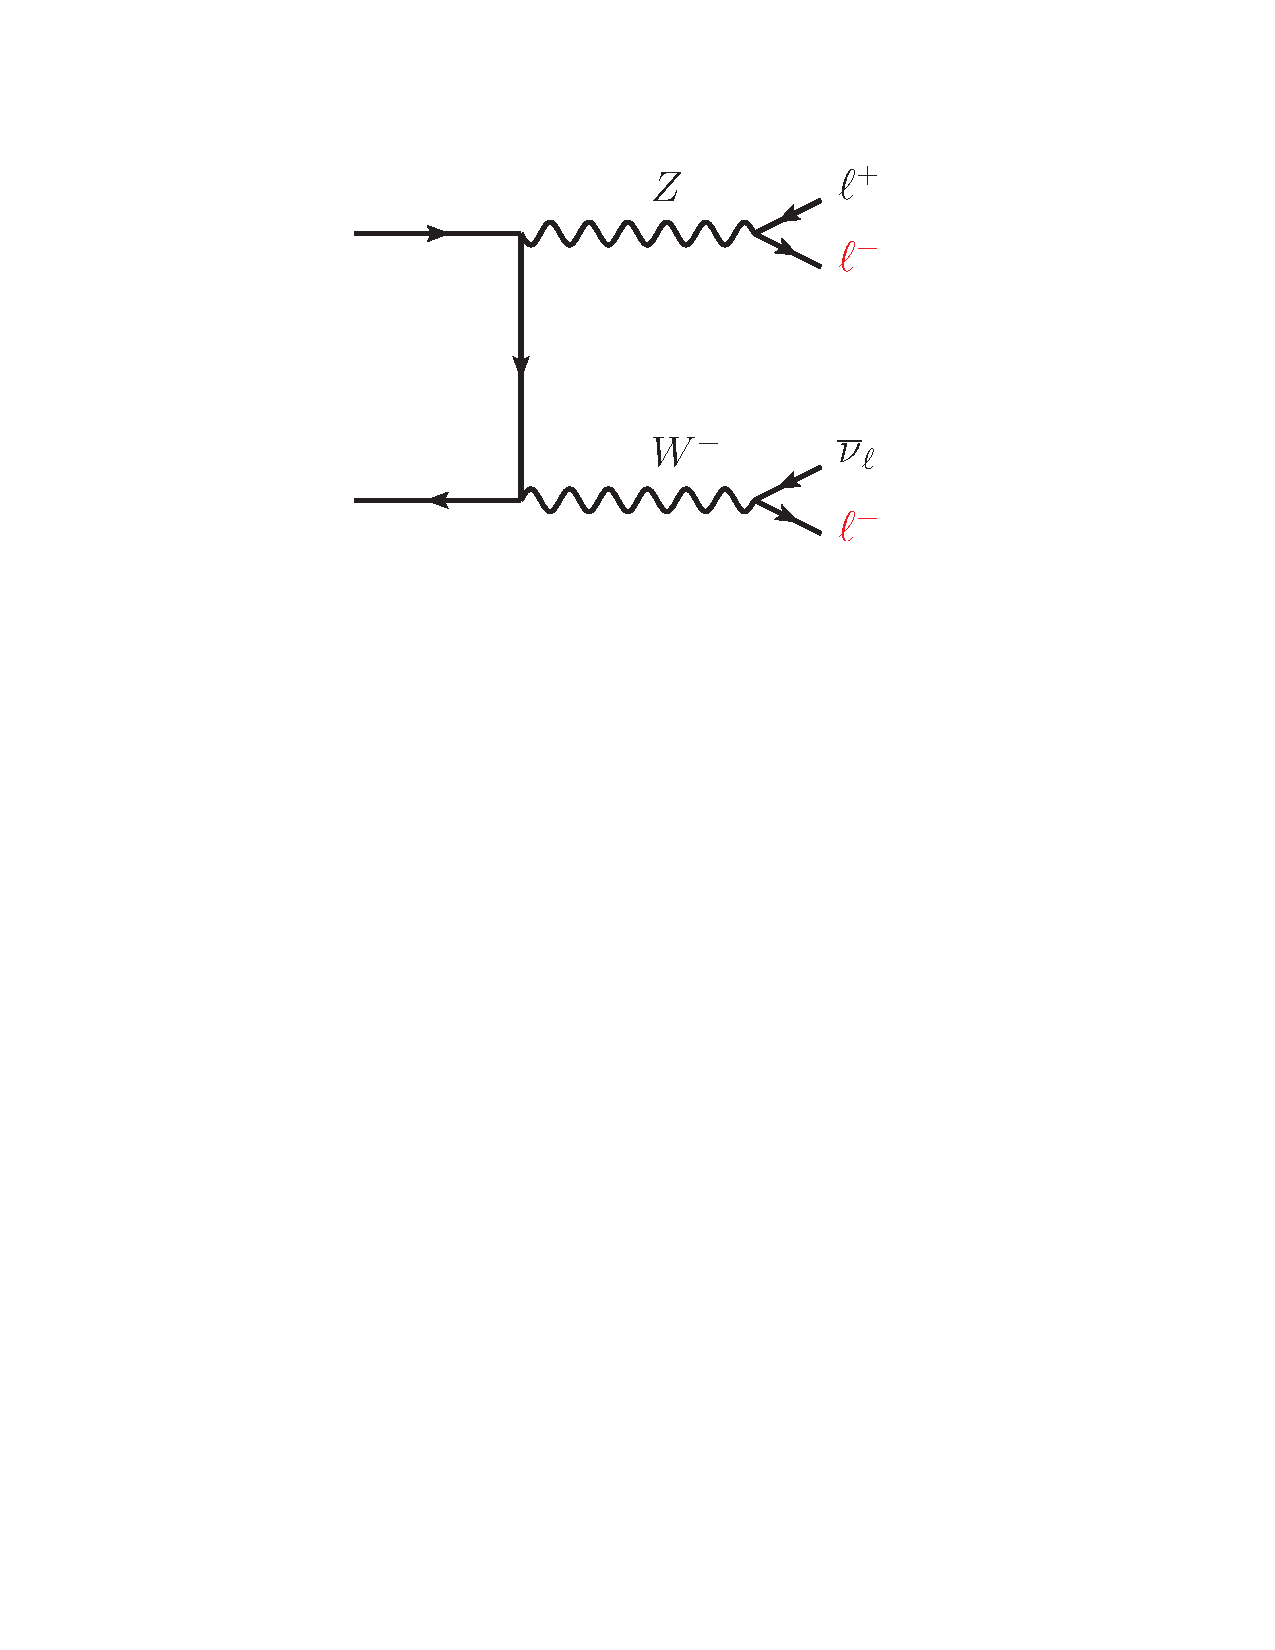
\includegraphics[width=0.8\textwidth, clip = true, trim = 1in 7.0in 1in 1in]{wz.pdf}
\caption[Feynman diagram for \WZ]
{\label{fig:feyn_wz}
Example leading order Feynman diagram for $pp \to \WZ \to 3\ell\nu + X$.
}
\end{center}
\end{figure}
% --------------------------------------------------------------------------- %
Processes than involve diboson production considered in this analysis are
listed below:
\begin{itemize}
\item \Wgamma: The $W$ and $\gamma$ decay leptonically ($W^{\pm} \to \ell^{\pm}\nu$ and $\Glplm$).
\item \WZ: The $W$ and $Z$ decay leptonically ($W^{\pm} \to \ell^{\pm}\nu$ and $\Zlplm$).
\item \ZZ: Both $Z$'s decay leptonically ($2 \times \Zlplm$).
\end{itemize}
 
% --------------------------------------------------------------------------- %
\subsection{Triple Gauge Boson Processes}
\label{sec:ss_rare_triboson}
% --------------------------------------------------------------------------- %

Processes involving the production of three electroweak bosons in the same
event can easily produce same-sign leptons. Producing three gauge boson is
considerably suppressed with respect to processes with two bosons since this
requires even more energy to produce due to the additional mass of the extra
boson. A typical example can be seen from the Feynman diagram shown in Figure
\ref{fig:feyn_vvv}.
% --------------------------------------------------------------------------- %
\begin{figure}[tbhp]
\begin{center}
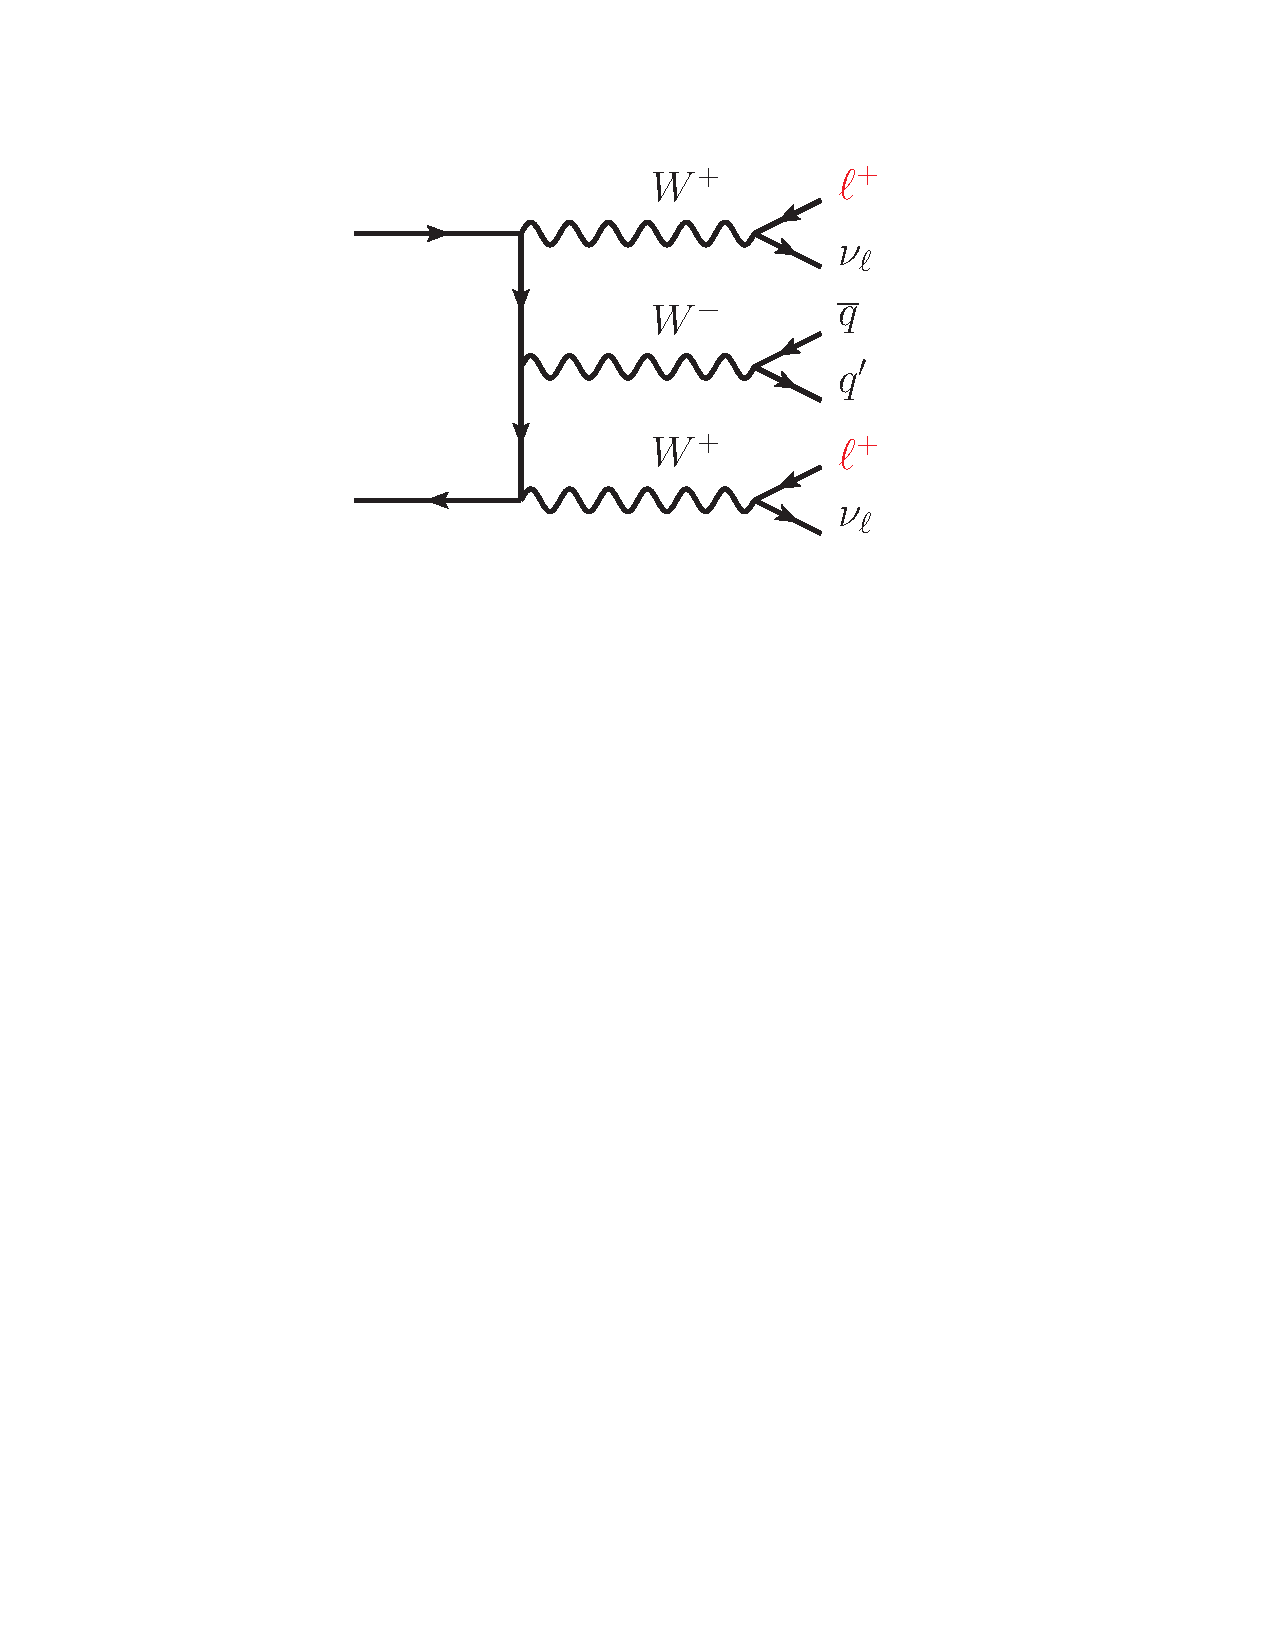
\includegraphics[width=0.8\textwidth, clip = true, trim = 1in 7.0in 1in 1in]{www.pdf}
\caption[Feynman diagram for \WZ]
{\label{fig:feyn_vvv}
Example leading order Feynman diagram for $pp \to \WWW$.
}
\end{center}
\end{figure}
% --------------------------------------------------------------------------- %
Processes that involve triboson production considered in this analysis are
listed below:
\begin{itemize}
\item \WWG: One or both $W$ bosons decay leptonically and the $\gamma$ decays leptonically ($\Wpmlpmnu$ and $\Glplm$).
\item \WWW: Two of the $W$ bosons with the same sign decay leptonically ($2 \times W^{+} \to \ell^{+}\nu_{\ell}$ or the charge conjugate).
\item \WWZ: One of the $W$ bosons and the $Z$ boson decay leptonically ($\Wpmlpmnu$ and $\Zlplm$).
\item \WZZ: Either the $W$ boson and at least one of the $Z$ bosons decay leptonically or both $Z$ bosons decay leptonically ($\Wpmlpmnu$ and at least one $\Zlplm$ or $2 \times \Zlplm$).
\item \ZZZ: At least two of the $Z$ bosons decay leptonically ($2\ \rm{or}\ 3 \times \Zlplm$).
\end{itemize}

% --------------------------------------------------------------------------- %
\subsection{Higgs Boson Processes}
\label{sec:ss_rare_higgs}
% --------------------------------------------------------------------------- %

Processes involving the Higgs boson production in conjunction with a $W$ or $Z$ boson or a top quark pair.
The Higgs can decay to W or Z bosons or tau leptons which can lead to same sign dileptons.
A typical example can be seen from the Feynman diagram shown in Figure \ref{fig:feyn_higgs} below:
% --------------------------------------------------------------------------- %
\begin{figure}[tbhp]
\begin{center}
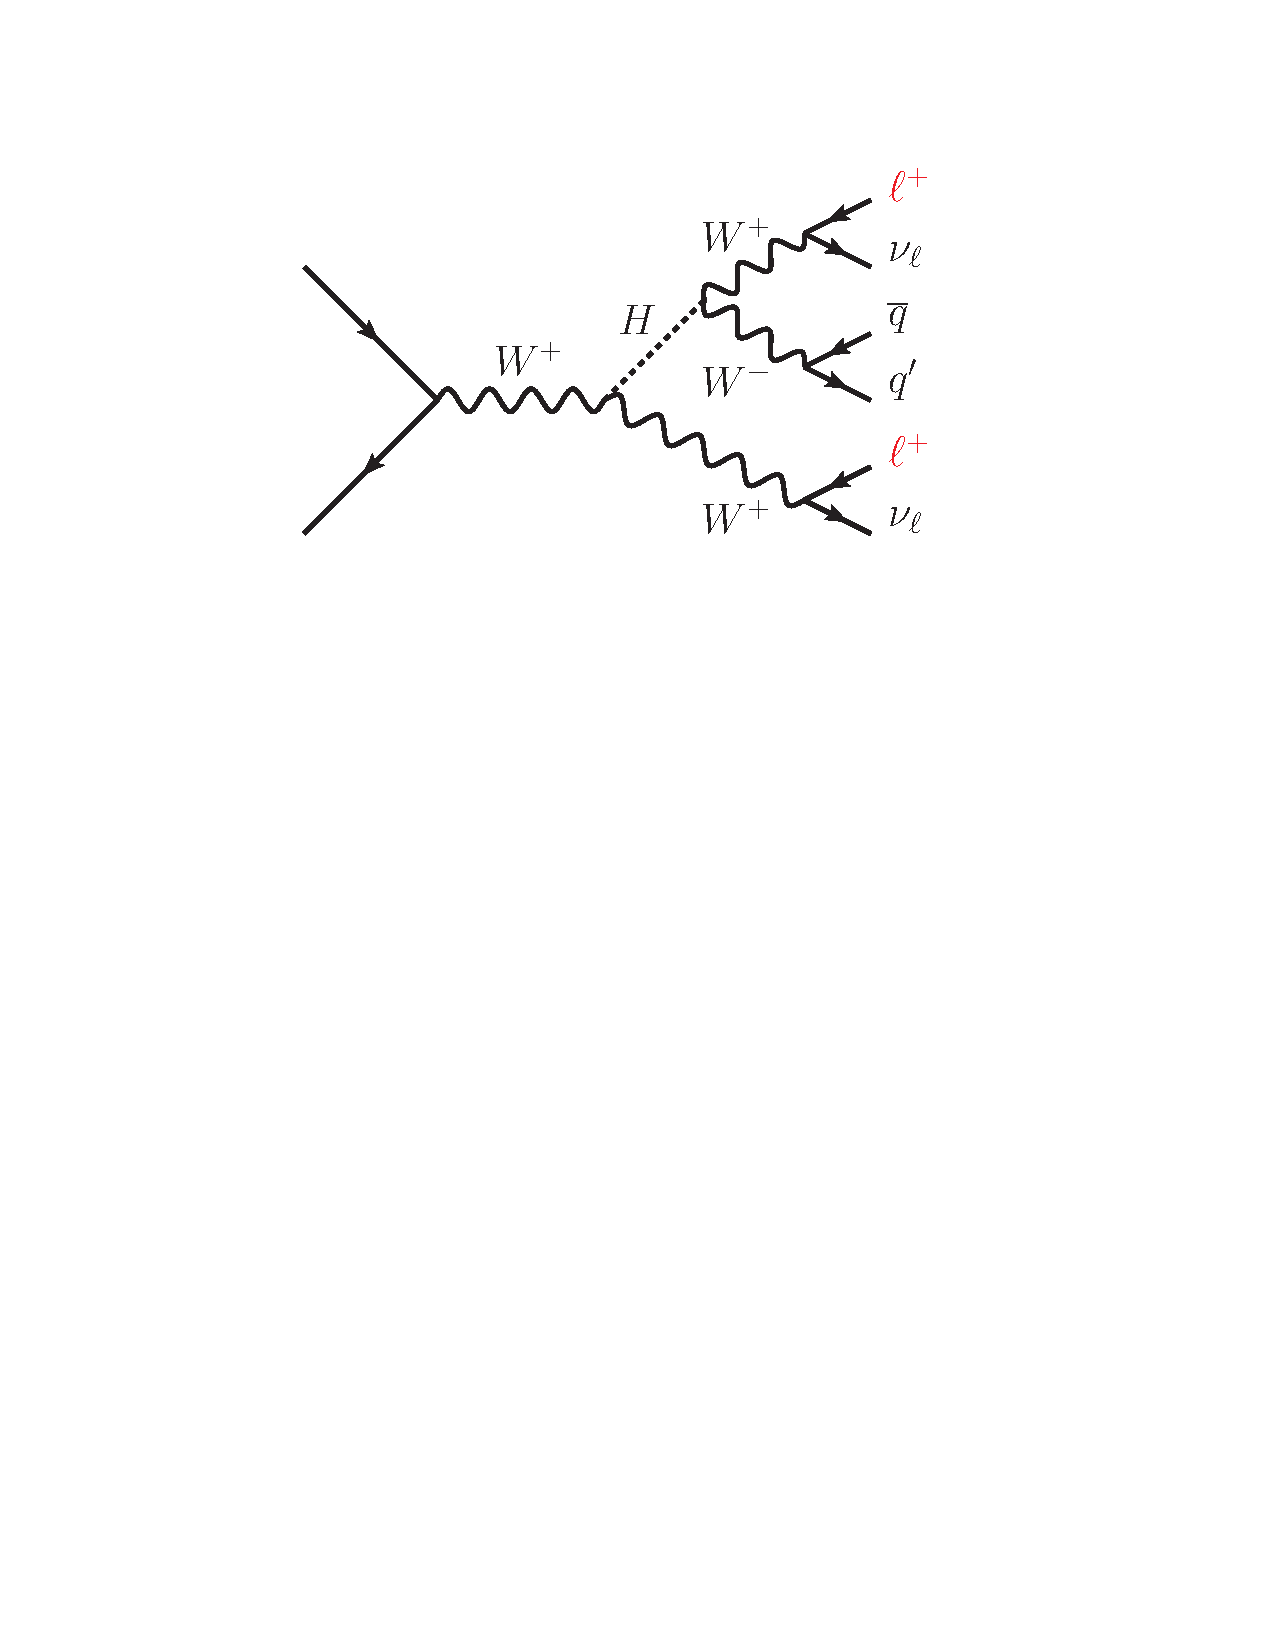
\includegraphics[width=0.8\textwidth, clip = true, trim = 1in 7.0in 1in 1in]{wh_hww.pdf}
\caption[Feynman diagram for \WZ]
{\label{fig:feyn_higgs} 
Example leading order Feynman diagram for $pp \to WH; H \to W^+W^-$.
}
\end{center}
\end{figure}
% --------------------------------------------------------------------------- %
Processes than involve associated Higgs Boson production considered in this analysis are
listed below:
\begin{itemize}
\item \HToWW: One lepton comes from the decay of the associated $W$, $Z$ or $\ttbar$ pair.  The other lepton comes from a leptonically decaying $W$ boson.
\item \HToZZ: One lepton comes from the decay of the associated $W$, $Z$ or $\ttbar$ pair.  The other lepton comes from a leptonically decaying $Z$ boson.
\item \HToTauTau: One lepton comes from the decay of the associated $W$, $Z$ or $\ttbar$ pair.  The other lepton comes from a leptonically decaying $\tau$ lepton.
\end{itemize}

% --------------------------------------------------------------------------- %
\subsection{Same-Sign W Boson Pair Production}
\label{sec:ss_rare_ssww}
% --------------------------------------------------------------------------- %

Processes involving the production of two bosons with the same electric charge
where both W's decay leptonically will also produce same-sign dileptons. The
two processes we consider for this situation include double parton scattering
(DPS) and $\qqWW$.
% --------------------------------------------------------------------------- %
\begin{figure}[tbhp]
\begin{center}
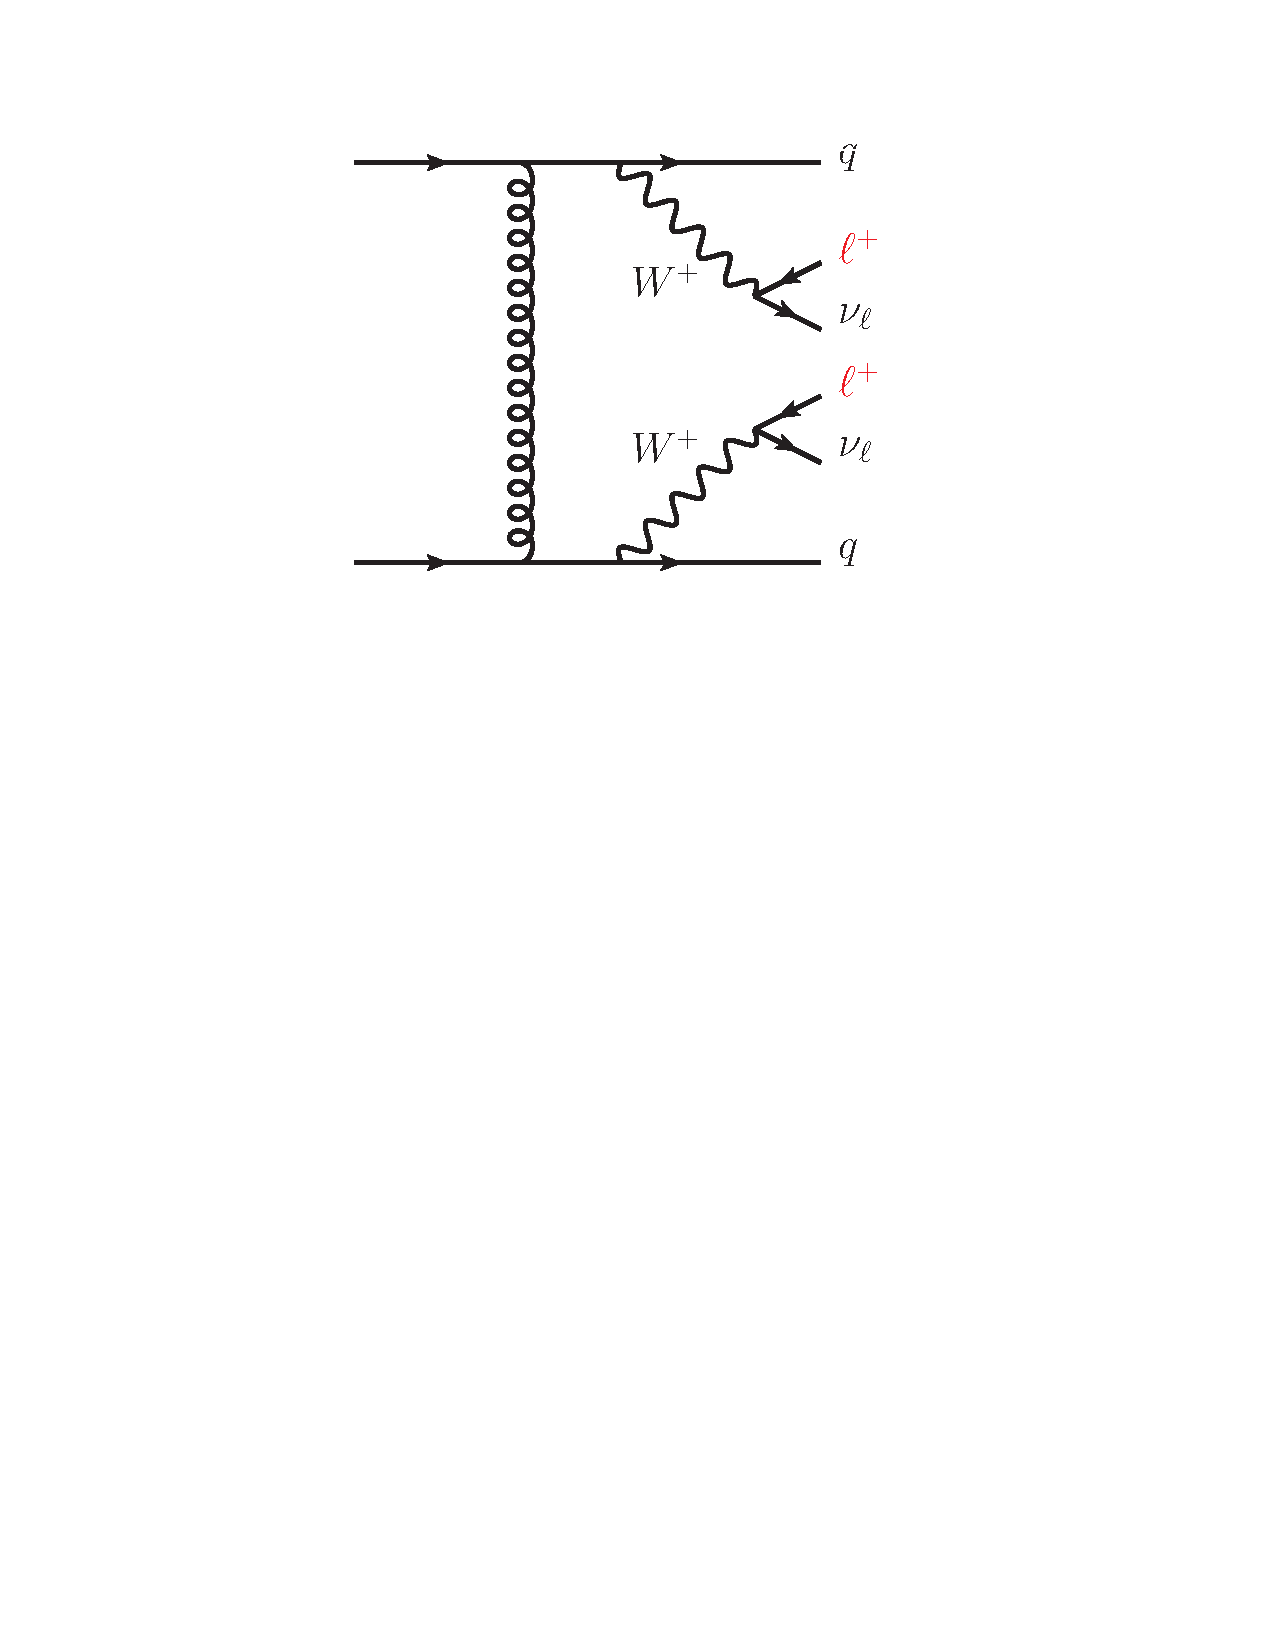
\includegraphics[width=0.8\textwidth, clip = true, trim = 1in 7.0in 1in 0.9in]{qqww.pdf}
\caption[Feynman diagram for \qqWW]
{\label{fig:feyn_ssww} 
Example leading order Feynman diagram for $\qqWW \to \ell^{\pm}\nu_{\ell}\ell^{\pm}\nu_{\ell} + qq$.
}
\end{center}
\end{figure}
% --------------------------------------------------------------------------- %
Processes than involve same-sign W pair production considered in this analysis are
listed below:
\begin{itemize}
\item \qqWW: Two same signed quarks are produced and each radiates a W boson which both decay leptonically ($pp \to qqWW$). 
\item \WWdps: Two independent hard parton collisions that both produce W bosons which both decay leptonically ($pp \to 2 \times \Wlnu$).
\end{itemize}

% --------------------------------------------------------------------------- %
% --------------------------------------------------------------------------- %
\section{Other Sources of Backgrounds}
\label{sec:ss_bkgd}
% --------------------------------------------------------------------------- %
% --------------------------------------------------------------------------- %
In the previous subsection, we discussed SM process that give rise to events
that posses genuine same-sign dileptons in the final state. In an ideal
scenario, this is all we would need to consider; however, there are two other
major sources of background that are caused by our inability to select the
correct events with 100\% certainty. The first of these is the non-negligible
situation when an electron or muon is reconstructed and mis-identified as a
prompt and isolated lepton. The second situation is less significant than the
first but nevertheless is still important and is accounted for. This is the
case where a real electron is reconstructed and selected; however, its electric
charge is mis-reconstructed. The following subsections will give a brief
discussion of these two cases, respectively.

% --------------------------------------------------------------------------- %
\subsection{Fake Leptons}
\label{sec:ss_bkgd_fakes}
% --------------------------------------------------------------------------- %

The dominant source of same-sign dileptons are events where one lepton is from
$\Wlnu$ and the other originates from a semi-leptonic b-quark decay. We refer
to leptons that originate from a electroweak boson or something with similar
properties (such as a super-symmetric object) as ``real leptons'' since these
give rise to true prompt and isolated leptons. For leptons that originate from
other sources, we refer to this as a ``fake lepton'' since this is not the
lepton we are interested in.

By far, the dominant source of fake leptons is $\ttbar$ events. A
representative diagram of this sort of event can be seen in the figure below
(Figure~\ref{fig:feyn_ttbar_fakes}).
% --------------------------------------------------------------------------- %
\begin{figure}[tbhp]
\begin{center}
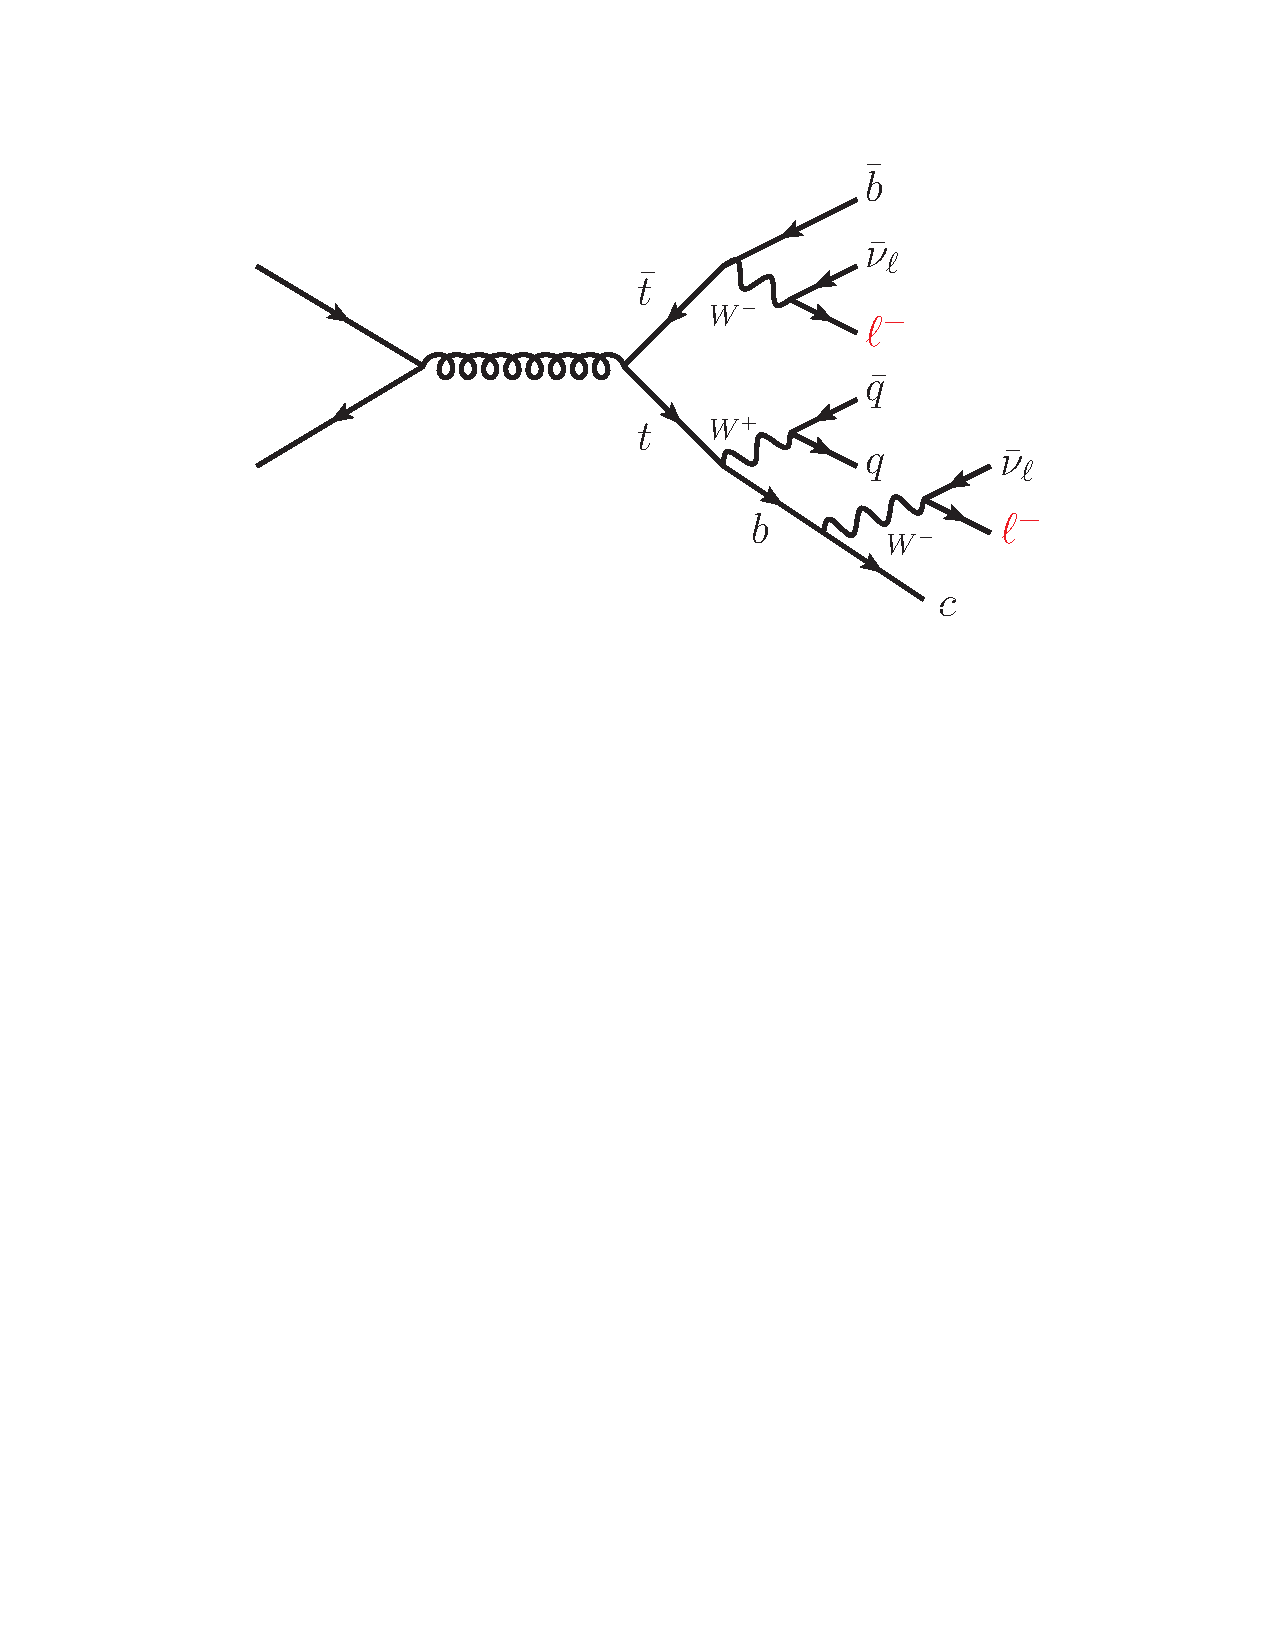
\includegraphics[width=0.8\textwidth, clip = true, trim = 1in 6.7in 1in 1in]{tt_fake.pdf}
\caption[Feynman diagram for fakes from \ttbar]
{\label{fig:feyn_ttbar_fakes} 
Diagram for \ttbar decays giving rise to same-sign dileptons final state.
}
\end{center}
\end{figure}
% --------------------------------------------------------------------------- %
Here we get a same-sign dilepton final state by having one of the leptons
from a top quark decaying leptonically from $\Wlnu$ and the other from
a ``fake'' lepton from the semi-leptonic b-quark decay from the other
top~\cite{an_ssb2011}. Anther important but sub-dominant source of fake lepton
background is from $pp \to \Wlnu + \text{jets}$ events where the jet decays
semi-leptonically.

The actual rate that the fake lepton will pass your analysis selection is
dependent on the details of the analysis. In Section \ref{sec:bkgd_fakes}, we
give a prediction on the number of same-sign dilepton event containing these
fake leptons.

% --------------------------------------------------------------------------- %
\subsection{Charge Flips}
\label{sec:ss_bkgd_flips}
% --------------------------------------------------------------------------- %

The measurement of a lepton's charge is determined from the curvature of the
reconstructed track as is travels through the magnetic field. The rate at which
the charge is mis-measured is negligibly small for muons at the W/Z momentum
scale; however, for electrons it is significant. Bremsstrahlung is emitted as
electrons are deflected by the silicon-based material of the track. A radiated
photon has a significant probability to covert into an \epem pair due to the
relatively large amount of material in the tracker~\cite{tdr1}. The combination
of the radiation of a hard photon and a subsequent asymmetric conversion (i.e.
when one of the two resulting electrons carries a significant fraction of the
momentum of the original photon) can result in the reconstruction of a track
that combines hits from the original electron with those from the converted
photon. As a result, the reconstructed track may have a curvature opposite to
that of the prompt electron, resulting in an incorrect charge assignment.

We estimate the rate that an electron that passes the analysis selection but
has an incorrect charge measurement to be $\sim 0.01\%$~\cite{an_ssb2013}.
The actual rate has been measured and will be fully discussed in Section
\ref{sec:bkgd_flips}.

% --------------------------------------------------------------------------- %
% --------------------------------------------------------------------------- %
\chapter{Analysis Selections}
\label{ch:evtsel}
% --------------------------------------------------------------------------- %
% --------------------------------------------------------------------------- %
In Chapter~\ref{ch:ss}, we discussed the motivation for selecting same-sign
dilepton pairs. In this Chapter, we discuss the specific selections used to
carry out the analysis. We consider a number of final states characterized
by the number of jets, number of b-tagged jets, scalar sum \pt~of selected
jets (\Ht) and the missing transverse energy (\met). To provide coverage for
a wide-range of generic signatures, we provide separate results for different
lepton \pt~requirements. Specifically, we perform a \hpt~analysis where we
select leptons with a \pt~requirement of 20 \GeV~(\hpt~analysis) as is common
for leptons from $W/Z$ and in many scenarios of stop/sbottom production. We
separately consider dilepton pairs where the \pt~requirement is lowered to 10
\GeV~(\lpt~analysis). This slightly looser selection provides sensitivity to
scenarios with a (partially) compressed spectrum, where at least one lepton
is expected to come from the decay of an off-shell $W/Z$. Finally, we define
search region in bins of \njets, \nbtags, \Ht and \met in order to improve
statistical sensitivity.

This chapter begins with a discussion on the collision and simulated data used
for this thesis. This is followed by the definitions of the selections for
all the physics objects used; and finally, this chapter concludes with the
discussion on the various search regions used in the analysis.

% --------------------------------------------------------------------------- %
% --------------------------------------------------------------------------- %
\section{Data Samples}
\label{sec:evtsel_samples}
% --------------------------------------------------------------------------- %
% --------------------------------------------------------------------------- %

% --------------------------------------------------------------------------- %
\subsection{Collision Data}
\label{sec:evtsel_samples_data}
% --------------------------------------------------------------------------- %
This analysis uses data collected during the 2012 run at $\sqrt{s} = 8\ \TeV$.
Dilepton events are selected from primary datasets collected using electron and
muon trigger paths. Only runs and luminosity sections from good data taking
periods are used, where such periods are defined using the flags delivered by
the CMS data quality monitoring, detector, and physics validation teams. The
datasets used in this analysis are listed in Tables~\ref{tab:evtsel_datasets_hpt},
and \ref{tab:evtsel_datasets_lpt} with the integrated luminosity corresponding to
\usedLumi.

% --------------------------------------------------------------------------- %
\begin{table}[hbt!]
\begin{center}
\caption[Primary datasets used by the \hpt analysis along with the relevant run-ranges]
{\label{tab:evtsel_datasets_hpt}
Primary datasets used by the \hpt analysis along with the relevant run-ranges.
}
\end{center}
\resizebox{0.78\textwidth}{!}{\begin{minipage}{\textwidth}
\begin{tabular}{lc}\hline\hline
Name                                                    & Run Range                          \\ \hline
{\tt /DoubleMu/Run2012A-13Jul2012-v1/AOD              } & 190456-193621                      \\ 
{\tt /DoubleMu/Run2012B-13Jul2012-v1/AOD              } & 193834-196531                      \\ 
{\tt /DoubleMu/Run2012A-recover-06Aug2012-v1/AOD      } & 190949 190945 190906 190895 190782 \\ 
{\tt /DoubleMu/Run2012C-24Aug2012-v1/AOD              } & 198022-198523                      \\ 
{\tt /DoubleMu/Run2012C-PromptReco-v2/AOD             } & 198934-203755                      \\ 
{\tt /DoubleMu/Run2012D-PromptReco-v1/AOD             } & 203773-208913                      \\ 
{\tt /DoubleElectron/Run2012A-13Jul2012-v1/AOD        } & 190456-193621                      \\ 
{\tt /DoubleElectron/Run2012B-13Jul2012-v1/AOD        } & 193834-196531                      \\ 
{\tt /DoubleElectron/Run2012A-recover-06Aug2012-v1/AOD} & 190949 190945 190906 190895 190782 \\ 
{\tt /DoubleElectron/Run2012C-24Aug2012-v1/AOD        } & 198022-198523                      \\ 
{\tt /DoubleElectron/Run2012C-PromptReco-v2/AOD       } & 198934-203755                      \\ 
{\tt /DoubleElectron/Run2012D-PromptReco-v1/AOD       } & 203773-208913                      \\ 
{\tt /MuEG/Run2012A-13Jul2012-v1/AOD                  } & 190456-193621                      \\ 
{\tt /MuEG/Run2012B-13Jul2012-v1/AOD                  } & 193834-196531                      \\ 
{\tt /MuEG/Run2012A-recover-06Aug2012-v1/AOD          } & 190949 190945 190906 190895 190782 \\ 
{\tt /MuEG/Run2012C-24Aug2012-v1/AOD                  } & 198022-198523                      \\ 
{\tt /MuEG/Run2012C-PromptReco-v2/AOD                 } & 198934-203755                      \\ 
{\tt /MuEG/Run2012D-PromptReco-v1/AOD                 } & 203773-208913                      \\ 
\hline\hline
\end{tabular}
\end{minipage} 
}
\end{table}
% --------------------------------------------------------------------------- %
\begin{table}[hbt]
\begin{center}
\caption[Primary datasets used by the \lpt analysis along with the relevant run-ranges]
{\label{tab:evtsel_datasets_lpt}
Primary datasets used by the \lpt analysis along with the relevant run-ranges.
}
\end{center}
\resizebox{0.8\textwidth}{!}{\begin{minipage}{\textwidth}
\begin{tabular}{lc}\hline
Name                                                 & Run Range                          \\ \hline
{\tt /MuHad/Run2012A-13Jul2012-v1/AOD              } & 190456-193621                      \\ 
{\tt /MuHad/Run2012B-13Jul2012-v1/AOD              } & 193834-196531                      \\ 
{\tt /MuHad/Run2012A-recover-06Aug2012-v1/AOD      } & 190949 190945 190906 190895 190782 \\ 
{\tt /MuHad/Run2012C-24Aug2012-v1/AOD              } & 198022-198523                      \\ 
{\tt /MuHad/Run2012C-PromptReco-v2/AOD             } & 198934-203755                      \\ 
{\tt /MuHad/Run2012D-PromptReco-v1/AOD             } & 203773-208913                      \\ 
{\tt /ElectronHad/Run2012A-13Jul2012-v1/AOD        } & 190456-193621                      \\ 
{\tt /ElectronHad/Run2012B-13Jul2012-v1/AOD        } & 193834-196531                      \\ 
{\tt /ElectronHad/Run2012A-recover-06Aug2012-v1/AOD} & 190949 190945 190906 190895 190782 \\ 
{\tt /ElectronHad/Run2012C-24Aug2012-v1/AOD        } & 198022-198523                      \\ 
{\tt /ElectronHad/Run2012C-PromptReco-v2/AOD       } & 198934-203755                      \\ 
{\tt /ElectronHad/Run2012D-PromptReco-v1/AOD       } & 203773-208913                      \\ 
\hline\hline
\end{tabular}
\end{minipage} 
}
\end{table}

% --------------------------------------------------------------------------- %
\subsection{Simulated Data}
\label{sec:evtsel_samples_mc}
% --------------------------------------------------------------------------- %
The analysis uses simulated data samples for candidate signal models and the
relevant backgrounds. The contributions for real same-sign dilepton events are
estimated directly from simulated data. These ``rare'' processes were discussed
in Chapter~\ref{sec:ss_rare} and constitute an irreducible background for
this analysis. Simulated samples of \Zgs, \Wj, and \ttbar processes are used to
cross-check the partially data-driven estimate of the background contribution
from charge mis-reconstruction, as well as systematic uncertainties of
the lepton selection. The data-driven technique developed to estimate the
background from fake leptons is applied to simulated \ttbar and \Wj samples
as part of the systematic uncertainty studies on these methods. Simulated SUSY
samples are used for the study of the systematic uncertainties as well as to
develop a model of the selection efficiencies. These samples are also used
in the extraction of upper limits on the observed and expected cross section
for these models. The contribution from double fakes from QCD processes is
determined using a data-driven method, but the available simulated samples
are used to study some dependencies of the fake lepton prediction method.
Simulated data samples are normalized to an integrated luminosity of \usedLumi,
unless otherwise stated. Details of the simulated samples can be found in
Tables~\ref{tab:evtsel_datasets_rare} and ~\ref{tab:evtsel_datasets_fake}.

% --------------------------------------------------------------------------- %
\begin{table}[!hbt]
\begin{center}
\caption[Sources of true same-sign dileptons from Standard Model processes]
{\label{tab:evtsel_datasets_rare}
Sources of true same-sign dileptons from Standard Model processes. Cross
sections are next-to-leading order. The equivalent integrated luminosity
of these simulated events is listed in the column on the far right. The
contributions from these process to the background is taken directly from
simulation.
}
\footnotesize{
    \begin{tabular}{lccc}
    \hline\hline
    Sample     & Cross Section (pb) & Equivalent Luminosity (\fbinv) \\ \hline
    \ttZ       & 0.208              & 1021                           \\
    \ttW       & 0.232              & 845                            \\
    \ttWW      & 0.00204            & 106931                         \\
    \ttG       & 2.17               & 33                             \\
    \tbZ       & 0.0114             & 13026                          \\
    \ZZZ       & 0.00554            & 40692                          \\
    \WWW       & 0.0822             & 2737                           \\
    \WWG       & 0.528              & 407                            \\
    \WZZ       & 0.0192             & 12946                          \\
    \WWZ       & 0.0580             & 3832                           \\
    \ZZ        & 0.177              & 27177                          \\
    \WZ        & 1.058              & 1908                           \\
    \qqWmWm    & 0.0889             & 1084                           \\
    \qqWpWp    & 0.248              & 402                            \\
    \WWdps     & 0.588              & 1418                           \\
    \Wgsmm     & 1.91               & 156                            \\
    \Wgstt     & 0.336              & 148                            \\
    \HToWW     & 0.260              & 769                            \\
    \HToZZ     & 0.0320             & 15652                          \\
    \HToTauTau & 0.0177             & 5478                           \\
    \hline\hline
    \end{tabular}
}
\end{center}
\end{table}
% --------------------------------------------------------------------------- %

% --------------------------------------------------------------------------- %
\begin{table}[!hbt]
\begin{center}
\caption[Sources of ``false`` same-sign dileptons from Standard Model processes]
{\label{tab:evtsel_datasets_fake}
Sources of ``fake`` same-sign dileptons from Standard Model processes. Cross
sections are next-to-leading order. The equivalent integrated luminosity
of these simulated events is listed in the column on the far right. The
contributions from these process to the background is taken directly from
simulation.
}
\footnotesize{
    \begin{tabular}{lccc}
    \hline\hline
    Sample                    & Cross Section (pb) & Equivalent Luminosity (\fbinv) \\ \hline
    \ttbar                    & 225                & 30                             \\
    \ttdil                    & 25                 & 493                            \\
    \ttslq                    & 103                & 248                            \\
    \tthad                    & 107                & 292                            \\
    $t$, s-channel            & 3.89               & 69                             \\
    $\overline{t}$, s-channel & 1.76               & 80                             \\
    $t$, s-channel            & 55.5               & 66                             \\
    $\overline{t}$, s-channel & 30.0               & 63                             \\
    $tW$                      & 11.2               & 45                             \\
    $overline{t}W$            & 11.2               & 44                             \\
    \Zgll                     & 3533               & 8.62                           \\
    \Wj                       & 37509              & varies                         \\
    \WW                       & 5.81               & 332                            \\
    \hline\hline
    \end{tabular}
}
\end{center}
\end{table}
% --------------------------------------------------------------------------- %

% --------------------------------------------------------------------------- %
\section{Event Selections}
\label{sec:evtsel_evt}
% --------------------------------------------------------------------------- %
% --------------------------------------------------------------------------- %
The event selection consists of the following general requirements with
amplifying details in the following sub-sections:
\begin{itemize}
\item we require a dilepton trigger;
\item we select events with two good same sign isolated leptons; the \hpt
analysis requires both leptons to have $\pt > 20~\GeV$ and the \lpt analysis
requires the leptons to have $\pt > 10~\GeV$.
\item $\m_{\ell\ell} > 8 \GeV$ to reject low mass resonances.
\item For most search regions, a significant amount of \met to reduce SM
backgrounds, particularly that from charge mis-measurement in \Zll events.
\item We require a significant amount of hadronic energy to reduce standard
model backgrounds, particularly mi-identified leptons in \Wj events.
\item We veto events if the invariant mass of either hypothesis lepton and a
third good lepton in the event is consistent with the Z mass. This requirement
is chosen to suppress the irreducible background from \WZ and \ZZ events.
\item We veto events if the invariant mass of either hypothesis lepton and a
third good lepton in the event is $< 12~\GeV$. This requirement is chosen to
suppress the irreducible background from \gs and low mass resonances.
\end{itemize}

To reject known machine background resulting in high activity in the pixel
layers, we require that no fewer than 25\% of the tracks in event are high
purity in events having 10 or more tracks. Also, to ensure that there was a
reconstructed collision, we require that at least on one good primary vertex
(PV). A good PV is selected by requiring:
\begin{itemize}
\item the PV is not considered a fake,
\item the number of degrees of freedom > 4,
\item $|\rho| < 2~\cm$,
\item $|z| < 24~\cm$.
\end{itemize}

% --------------------------------------------------------------------------- %
\subsection{Trigger Selection}
\label{sec:evtsel_trig}
% --------------------------------------------------------------------------- %
We use a handful of double lepton trigger paths to select events in data. An
event in the \ee final state is required to pass the relevant double electron
trigger, a \mm event must pass the double muon trigger and an \em event is
required to pass one of the electron-muon cross triggers. Because of the
rapidly changing trigger menu, many trigger paths were not implemented in the
simulation and thus no trigger requirement is made here. Instead, as discussed
in Section~\ref{sec:eff_trig}, a weight is applied to each event, based on the
trigger efficiencies measured from data. A list of trigger paths used to select
signal-like events can be found in in the following table:

% --------------------------------------------------------------------------- %
\begin{table}[!hbt]
\begin{center}
\caption[The trigger paths used for the \hpt and \lpt analyses]
{\label{tab:evtsel_trig}
The trigger paths used for the \hpt and \lpt analyses. Note that for the \hpt
triggers, {\tt XXLstr} stands for {\tt CaloIdT\_CaloIsoVL\_TrkIdVL\_TrkIsoVL}
which is explained in the text below. For the \lpt triggers, {\tt PFHT175} refers to
particle flow based $\Ht > 175 \GeV$.
}
\begin{tabular}{l|c|c}
\hline\hline
Analysis Type         & Channel & Trigger                                                   \\ \hline
\multirow{3}{*}{\hpt} & \ee & {\tt HLT\_Ele17\_XXLstr\_Ele8\_XXLstr}                        \\
                      & \em & {\tt HLT\_Mu17\_Ele8\_XXLstr} or {\tt HLT\_Mu8\_Ele17\_XXLstr}\\
                      & \mm & {\tt HLT\_Mu17\_Mu8}                                          \\ \hline
\multirow{3}{*}{\lpt} & \ee & {\tt HLT\_DoubleEle8\_CaloIdT\_TrkIdVL\_Mass8\_PFHT175}       \\
                      & \em & {\tt HLT\_Mu8\_Ele8\_CaloIdT\_TrkIdVL\_Mass8\_PFHT175}        \\
                      & \mm & {\tt HLT\_DoubleMu8\_Mass8\_PFHT175}                          \\
\hline\hline
\end{tabular}
\end{center}
\end{table}

% --------------------------------------------------------------------------- %
The \hpt analysis select event with two leptons having $\pt > 20\ \GeV$.
Dielectron events in the \hpt triggers are selected using triggers with
\Et requirements of 17 and 8 \GeV on the two legs. Triggers with electron
legs impose online calorimeter and tracker identification and isolating
requirements. The online selections are sufficiently loose compared to the
analysis isolation selection that little inefficiency is introduced. However,
care must be taken in the data-driven background estimate so that a bias is not
introduced. This issue was studied in detail elsewhere and found to not be a
significant concern~\cite{an_ufl2013}. The electron-muon cross triggers have
muon \pt requirements of 17 \GeV (8 \GeV) and corresponding \Et requirements of
8 \GeV (17 \GeV). The dimuon triggers have only a \pt requirement of
17 and 8 \GeV on the two legs.

The trigger paths used for the \lpt analyses have lower \pt
requirements due to the lower threshold on the lepton (i.e.~$\pt > 10\ \GeV$);
however, they impose an additional \HT requirement to keep the rate within the
allotted bandwidth. The online \HT requirement was 175 \GeV using particle flow
based jets. Later runs also imposed a pile-up correcting to the \HT calculation.
All three channels use triggers that also impose a dilepton invariant mass of
8 \GeV. The dielectron triggers have an \Et requirement of 8 \GeV on both
lets. Unlike the \hpt triggers, the electron legs impose only calorimeter
and tracker identification requirements -- no isolation requirement. The
electron-muon cross triggers require the same identification requirements on
the electron leg and select electrons with $\Et > 8\ \GeV$ and muons with $\pt
> 8\ GeV$. The \pt requirement in the dimuon trigger is 8 \GeV on both legs.

% --------------------------------------------------------------------------- %
\subsection{Muon Selection}
\label{sec:evtsel_mu}
% --------------------------------------------------------------------------- %
Muon reconstruction was discussed previously in Section~\ref{sec:cms_muon}. To reject
fakes with relatively little loss in efficiency, we require muons to be
reconstructed as both global muons and particle flow muons. To further
reject fakes and poorly reconstructed muons we apply the following quality
requirements~\cite{an_ssb2013,muonidtwiki}:
% --------------------------------------------------------------------------- %
\begin{itemize}
\item We require the muon to have $\pt > 20\ \GeV$ and $\pt > 10\ \GeV$ for the
\hpt and \lpt analysis, respectively.
\item We require the muon to have $|\eta| < 2.4$ which is the edge of the
muon detector coverage. Due to the finite luminous region, some muons can
have a track with $|\eta| > 2.4$; however, we do not consider these as the
inefficiency is relatively large.
\item We require that the global fit of the muon have $\chi^2/\rm{ndof} < 10$
to reject poorly reconstructed muons.
\item We require that at least one muon sub-detector hit is used in the global
fit.
\item We require that at least one hit is in the pixel layers.
\item We require that the muon have at least 6 layers in the silicon tracker,
to reject poorly reconstructed muons as well as muons originating late in the
tracker from decays in flight.
\item We require that the energy deposits in the veto cones are less that
4 \GeV in the ECAL and 6 \GeV in the HCAL. Veto deposits are calculated in
cones of size $\DR = 0.07,\ 0.1$ for the ECAL and HCAL, respectively. Vetoing
on the energy in the cones rejects fake muons produced when hadrons punch
through the calorimeter into the muon system. The requirement can introduce
an inefficiency for muons with \hpt or in a busy event environment such as a
\ttbar-like event~\cite{an_098_2008}.
\item We require the muon to have at least two segments in the muon chambers,
to reject reconstructed objects that are mis-identified as muons because they
punched through the calorimeter and interacted in the first layer of the
muons system (e.g. from kaons).
\item We require that the muon have transverse impact parameter (\dzero) $< 50\
\um$, where the \dzero has been calculated with respect to the primary vertex.
A tight selection reduces background muons from the decay of b-hadrons, as well
as decays in flight.
\item We require that the inner track $z$ be less than 1 mm from the first good
vertex, which we take to be the event vertex. This requirement helps reject
mis-reconstructed muons as well as those originating from pile-up interactions.
\end{itemize}
% --------------------------------------------------------------------------- %
The isolation follows the POG recommendation, using particle-flow based        
isolation with a $\Delta\beta$ correction for PU. However, a smaller cone      
size of \DR\ $=$ 0.3 is adopted due to the high hadronic activity expected in  
signal-like events. The isolation is calculated using                             
% --------------------------------------------------------------------------- %
$$
\relIso = [ \Sigma_{\rm ch} + {\rm max}(0, \Sigma_{\rm nh} + \Sigma_{\rm ph} - 0.5 \Delta\beta) ]/\pt,
$$
% --------------------------------------------------------------------------- %
where $\Sigma_{\rm ch, nh, ph}$ are the sums of the \pt of the charged hadron,
neutral hadron, and photon particle flow candidates, respectively. Here the
charged hadrons are matched to the PV and a 0.5~\GeV threshold is applied
on neutral hadrons and photons. The $\Delta\beta$ correction is determined
from the sum \pt\ of charged hadrons not matched to the PV with a threshold of
0.5~\GeV\ in a cone of the same size as the isolation. The \relIso is required
to be less than 0.1~\cite{muonpfisotwiki}.
% --------------------------------------------------------------------------- %
\subsection{Electron Selection}
\label{sec:evtsel_el}
% --------------------------------------------------------------------------- %
Electrons in this analysis are reconstructed using the Gaussian Sum Filter
(GSF) algorithm as was discussed in Section~\ref{sec:cms_electron}. For this analysis we
require the GSF electrons to passed the additional requirements:
% --------------------------------------------------------------------------- %
\begin{itemize}
\item We require the electron to have $\pt > 20\ \GeV$ and $\pt > 10\ \GeV$ for
the \hpt and \lpt analyses, respectively.
\item We require the electron to have $|\eta| < 2.4$.
\item We require the number of missing expected inner hits to be zero.
\item We require the $H/E < 0.1\ (0.075)$ in the barrel (endcap) to match the
requirements on the trigger.
\item We require that the electron have a $|\dzero| < 100\ \um$, where the
\dzero has been calculated with respect to the primary vertex. A tight
selection on the impact parameter reduces background from fake electrons and
electrons from photon conversions in the tracker.
\item We require that there is no muon within a cone of $\DR = 0.1$ about the
electron. Only muons passing the selection in Section~\ref{sec:evtsel_mu} are
considered. This veto rejects the situation where a muon is mis-reconstructed
as an electron.
\item We require the electron to pass the VBTF80 identification (see
Table~\ref{tab:evtsel_elid}).
\item We reject electrons with a supercluster \aeta in the transition region
between the barrel and endcap of the ECAL ($1.4442 < |\eta_{SC}| < 1.566$).
Electrons in this region are poorly reconstructed.
\item We require that the GSF track $z$ be less than 1 mm from the first
good vertex, which we take to be the event vertex. This requirement helps
reject mis-reconstructed electrons as well as those originating from pile-up
interactions.
\item We require that all three charge measurements for an electron agree.
One charge comes from the curvature of the GSF track. A second comes form the
curvature of the associated CTF track. We require all electrons to have an
associated CTF track. The last charge, the so-called supercluster charge, is
determined using the relative position of the supercluster with respect to the
projected track from the pixel seed.
\item To reject conversions, we apply a veto of a good reconstructed conversion
vertex. A conversion vertex is considered good if it has no tracker hits
towards the beam, has a fit probability above $10^{-6}$, has a displacement of
more than 2 \cm, and the CTF track matching to the electron should be a part
of the conversion vertex. No requirement is made on the vertex quality flag
corresponding to merging and arbitration.
\end{itemize}
% --------------------------------------------------------------------------- %
The isolation follows the POG recommendation, using particle-flow based
isolation with a cone size of $\DR = 0.3$~\cite{egammapfisotwiki}. In the
endcap, an inner veto of \DR\ $=$ 0.015 (0.08) is imposed for charged hadrons
(photons). The isolation is corrected for PU by subtracting from the neutral
isolation components a term defined by the product of the average event energy
density and the effective area of the isolation cone~\cite{egammaisorhoaeff}.
The neutral component after correction is required to be non-negative. The
isolation relative to the electron \pt\ is required to be less than 0.09.

The VBTF80 identification uses the selection from Table~\ref{tab:evtsel_elid}.
CMS defines the barrel/endcap transition to be at $|\eta_{SC}| = 1.479$.
The selection values are chosen to have approximately 80\% efficiency for
the electrons from W and Z decays. The values reported are from CMS
recommended values~\cite{egammaidtwiki}.
% --------------------------------------------------------------------------- %

\begin{table}[!hbt]
\begin{center}
\caption[Details of the modified VBTF80 electron identification]
{\label{tab:evtsel_elid}
Details of the modified VBTF80 electron identification.
}
\begin{tabular}{l|c|c}
\hline\hline
Selection Variable & Selection Value (barrel) & Selection Value (endcap) \\ \hline
\sieie             & < 0.01                   & < 0.03                   \\ 
$\dphi_{in}$       & < 0.06                   & < 0.03                   \\ 
$\eta{in}$         & < 0.004                  & < 0.007                  \\ 
$H/E$              & < 0.1                    & < 0.075                  \\ \cline{2-3}
$(1/E - 1/P)$      & \multicolumn{2}{c}{> 0.05}                          \\ 
\hline\hline
\end{tabular}
\end{center}
\end{table}
% --------------------------------------------------------------------------- %
The \sieie variable cuts on the energy deposits in the ECAL, electrons have
a characteristic shower shape that is narrow in $\eta$ but wide in
$\phi$, the latter due to the bremsstrahlung in the tracker of the electrons.
The $\dphi_{in}$ and $\deta_{int}$ variables are cut on the track-to-cluster
matching. The final variable, $H/E$, is calculated as a ratio of energies in
the ECAL and HCAL veto cones. An electron is expected to deposit nearly all of
its energy in the ECAL, while a hadron usually deposits significant energy in
the HCAL, as well.

% --------------------------------------------------------------------------- %
\subsection{Lepton Pair Disambiguation}
\label{sec:evtsel_pair}
% --------------------------------------------------------------------------- %
In events with multiple same-sign lepton pairs passing the selection above,
only one pair is selected according to the following prescription:
\begin{itemize}
\item We give preference to \mm pairs over \em, which are chosen over \ee pairs.
\item If multiple candidates remain, the pair with the highest scalar sum \pt is chosen.  
\end{itemize}

% --------------------------------------------------------------------------- %
\subsection{Jet Selection}
\label{sec:evtsel_jets}
% --------------------------------------------------------------------------- %
We require the presence of energetic hadronic activity in the event as new
physics with a large cross section is expected to be produced via the strong
interaction. We choose to use jets built from particle-flow candidates, as
they provide the best scale and resolution for jets typical of those produced
in SM process such as \ttbar events. Particle-flow candidate reconstruction
was discussed in section Section~\ref{sec:cms_pf} and jet reconstruction was
discussed in Section~\ref{sec:cms_jets}.
% --------------------------------------------------------------------------- %

\begin{table}[!hbt]
\begin{center}
\caption[Details of the loose particle flow identification]
{\label{tab:evtsel_jetid}
Details of the loose particle flow identification. From~\cite{an_003_2010}.
}
\begin{tabular}{l|c|c}
\hline\hline
Selection Variable                           & Selection Value & Comment       \\ \hline
fraction of energy from neutral hadrons      & < 0.99          &               \\ 
fraction of energy from neutral EM particles & < 0.99          &               \\ 
number of particle flow candidates           & > 1             &               \\ 
fraction of energy from charged hadrons      & > 0             & $\aeta < 2.4$ \\ 
fraction of energy from charged EM particles & < 0.99          & $\aeta < 2.4$ \\ 
number of charged particle flow candidates   & > 0             & $\aeta < 2.4$ \\ 
\hline\hline
\end{tabular}
\end{center}
\end{table}
% --------------------------------------------------------------------------- %
Jets are reconstructed with the anti-$k_T$ algorithm with parameter $R =
0.5$. Jets in simulation have L1FastJetL2L3 corrections applied, as well as
jets in data have L2L3 residual corrections applied~\cite{jetcorrtwiki}.
Selected jets are required to pass the loose particle flow jet ID described
in Table~\ref{tab:evtsel_jetid}. These selections are very loose and are
primarily intended to reject jets that are unambiguously due to detector
noise. The inefficiency of this selection on simulation is less than
1\%~\cite{an_003_2010}. Additionally, jets are required to be separated by $\DR
> 0.4$ from any hypothesis leptons and other leptons passing the selection
above.

In the event, there must be at least two particle-flow jets with $\pt > 40\
\GeV$ and $\aeta < 2.4$. The fiducial cut coincides with the extent of the
tracker. In addition to counting jets, the analysis also makes a selection
based on the total hadronic activity in the event, \Ht. The \Ht is calculated
as the scalar sum of the \pt of all jets passing the jet counting criteria
discussed above. Even a modest \Ht requirement suppresses the background from
failures of lepton identification in \Wj events. Having two jets in the event
imposes a minimal \Ht requirement of 80 \GeV.

% --------------------------------------------------------------------------- %
\subsection{B-Tagging Selection}
\label{sec:evtsel_btag}
% --------------------------------------------------------------------------- %
Jets selected based on the requirements of Section~\ref{sec:evtsel_jets} are
b-tagged using the Combined Secondary Vertex method with the medium working
point (CSVM) tagger. This tagger identifies jets with discriminant larger
than 0.679 as b-tagged. The details of b-jet identification was discussed in
Section~\ref{sec:cms_btags}.

% --------------------------------------------------------------------------- %
\subsection{Missing Transverse Energy Selection}
\label{sec:evtsel_met}
% --------------------------------------------------------------------------- %
Missing transverse energy is a natural requirement for new physics searches.
Many models contain weakly interacting particles. For example, some of the
SUSY models considered produce leptons via decay chains ending in a lightest,
non-interacting particle (LSP). CMS uses three different \met reconstruction
algorithms; however, for this analysis, we use \met reconstructed from a
vector sum of the particle flow candidates which was discussed in detail in
Section\ref{sec:cms_met}. For almost all of the search scenarios, we impose a
minimum \met requirement of at least 30 \GeV. Event a modest \met requirement
is effective at suppressing background from Drell-Yan process in the \ee and
\em final states where the charge on one of the final state electrons is
mis-reconstructed.

% --------------------------------------------------------------------------- %
\subsection{Z and $\gamma$* veto}
%[Z and Gamma* veto]
\label{sec:evtsel_zveto}
% --------------------------------------------------------------------------- %
One of the primary irreducible backgrounds to the same-sign dilepton search
comes from \WZ and \ZZ production, where the bosons both decay to leptons.
A natural same sign hypothesis is formed using a lepton from each of the
two bosons. In the case of the \WZ, the lepton from the $W$ comes together
with a neutrino of the same flavor providing a natural source of \met. To
reduce this background, we reject events for which one of the hypothesis
leptons and a third lepton in the event have an invariant mass consistent
with the $Z$, defined to be between 76 and 106 \GeV. Along the same lines, to
reject events with a virtual photon, we also require the invariant mass to
be less than 12 \GeV. We require the third lepton to be the same flavor and
opposite sign and to pass the identification and isolation criteria described
in Sections~\ref{sec:evtsel_el} and~\ref{sec:evtsel_mu}.

% --------------------------------------------------------------------------- %
% --------------------------------------------------------------------------- %
\section{Search Regions}
\label{sec:evtsel_sr}
% --------------------------------------------------------------------------- %
% --------------------------------------------------------------------------- %
As in previous versions of this
analysis~\cite{an_ssb2011,an_ssb2012,an_ssb2012hcp}, there is a minimal
baseline selection asking for a same-sign lepton pair and at least two jets
(or b-tagged jets). Here, we define separately a control region (baseline)
selection for each of the two lepton selections (\hpt and \lpt) in the
following b-tagged categories:
% --------------------------------------------------------------------------- %
\begin{itemize}
\item no \bj requirement,
\item require exactly one \bj,
\item require two or more \bjs.
\end{itemize}
% --------------------------------------------------------------------------- %
In the baseline regions, a relatively low \met requirement is made in an
effort to be inclusive to a wide variety of signatures such as same-sign top
productions or models with R-parity violation. Specifically, for R-parity
violating models we expect events that have many high \pt jets. Thus a
relatively high $\Ht>500\ \GeV$ requirement is required when searching for
this signature and any \met requirement is relaxed. Many of the viable models,
however, involve leptons arising from $W$ decays and thus naturally have \met
from the accompanying neutrino. To improve sensitivity to these signatures,
a region with $\met > 30 \GeV$ is introduced when $\Ht<500\ \GeV$. Table
\ref{tab:evtsel_srbl} summarizes the baseline search regions used in this
analysis where we define baselines for each of the analysis types. There are
a total of six baseline regions. For convenience, each search region is a
assigned a number, given in the far right column.

% --------------------------------------------------------------------------- %
\begin{table}[htb!]
\begin{center}
\caption[Summary of the baseline search regions considered in the \hpt and \lpt analysis]
{\label{tab:evtsel_srbl}
Summary of the baseline search regions considered in the \hpt and \lpt analysis.
}
\end{center}
\resizebox{0.7\textwidth}{!}{\begin{minipage}{\textwidth}
\begin{tabular}{c|c|c|c|c|c|c}
\hline\hline
Analysis              & min lepton \pt ($\mu$, e) (\GeV) & \Ht (\GeV)           & \met (\GeV)                               & \njets             & \nbtags & Search Region \# \\ \hline
\multirow{3}{*}{\hpt} & \multirow{3}{*}{20, 20}          & \multirow{3}{*}{80}  & \multirow{3}{*}{30 if $\Ht < 500$ else 0} & \multirow{3}{*}{2} & $\ge$ 0 & SR0              \\ \cline{6-7}
                      &                                  &                      &                                           &                    & = 1     & SR10             \\ \cline{6-7}
                      &                                  &                      &                                           &                    & $\ge$ 2 & SR20             \\ \hline
\multirow{3}{*}{\lpt} & \multirow{3}{*}{10, 10}          & \multirow{3}{*}{250} & \multirow{3}{*}{30 if $\Ht < 500$ else 0} & \multirow{3}{*}{2} & $\ge$ 0 & SR0              \\ \cline{6-7}
                      &                                  &                      &                                           &                    & = 1     & SR10             \\ \cline{6-7}
                      &                                  &                      &                                           &                    & $\ge$ 2 & SR20             \\ \hline
\end{tabular}
\end{minipage}
}
\end{table}  

% --------------------------------------------------------------------------- %
In contrast from the fall analysis, this analysis is performed as a
simultaneous counting experiment in multiple independent bins or search
regions. The search regions are defined by event selections on the lepton
\pt, \Ht, \met, \njets, and \nbtags. To improve sensitivity to SUSY scenarios
involving top and bottom squark production, we define regions with tighter \Ht
and \met requirements. The \met-\Ht plane is divided into 4 major regions:
% --------------------------------------------------------------------------- %
\begin{itemize}
	\item Low-\Ht~Low-\met~region: $200\ \GeV < \Ht < 400\ \GeV$, $50\ \GeV < \met < 120\ \GeV$.
	\item Low-\Ht~high-\met~region: $200\ \GeV < \Ht < 400\ \GeV$, $\met > 120\ \GeV$.
	\item high-\Ht~Low-\met~region: $\Ht > 400\ \GeV$, $50\ \GeV < \met < 120\ \GeV$.
	\item High-\Ht~high-\met~region: $\Ht > 400\ \GeV$, $\met > 120\ \GeV$.
\end{itemize}

% --------------------------------------------------------------------------- %
As will be discussed in Section~\ref{sec:results_int} all of the SUSY scenarios that we
consider explicitly have at least two quarks, zero to four b-quarks, up to two
hadronically decaying W bosons, and at least two neutrinos and two LSPs. Thus,
in all search regions, we require at least 2 jets but the \njets requirement is
broken into two categories:
% --------------------------------------------------------------------------- %
\begin{itemize}
\item two to three jets
\item four or more jets 
\end{itemize}
% --------------------------------------------------------------------------- %
Additionally, the SUSY inspired search regions also have exclusively defined
values on the \nbtags with exactly zero, exactly one and two or more b-tagged
jets.
% --------------------------------------------------------------------------- %
The search regions for the \hpt analysis are summarized in
Table~\ref{tab:evtsel_sr_hpt}.

\begin{table}[!htb]
\begin{center}
\caption[Search regions selected for the high \pt analysis]
{\label{tab:evtsel_sr_hpt}
Search regions selected for the high \pt search where we require $\Ht>200\ \GeV$.
}
\begin{tabular}{c|c|c|c|c}
\hline\hline
\nbtags                   & \met                    & \njets   & \Ht[200-400] & \Ht[$>400$] \\ \hline
\multirow{4}{*}{$=0$}     & \multirow{2}{*}{50-120} & 2-3      & SR1          & SR2         \\ \cline{3-5}
                          &                         & $\geq 4$ & SR3          & SR4         \\ \cline{2-5}
                          & \multirow{2}{*}{$>120$} & 2-3      & SR5          & SR6         \\ \cline{3-5}
                          &                         & $\geq 4$ & SR7          & SR8         \\ \hline
\multirow{4}{*}{$=1$}     & \multirow{2}{*}{50-120} & 2-3      & SR11         & SR12        \\ \cline{3-5}
                          &                         & $\geq 4$ & SR13         & SR14        \\ \cline{2-5}
                          & \multirow{2}{*}{$>120$} & 2-3      & SR15         & SR16        \\ \cline{3-5}
                          &                         & $\geq 4$ & SR17         & SR18        \\ \hline
\multirow{4}{*}{$\geq 2$} & \multirow{2}{*}{50-120} & 2-3      & SR21         & SR22        \\ \cline{3-5}
                          &                         & $\geq 4$ & SR23         & SR24        \\ \cline{2-5}
                          & \multirow{2}{*}{$>120$} & 2-3      & SR25         & SR26        \\ \cline{3-5}
                          &                         & $\geq 4$ & SR27         & SR28        \\ \hline\hline
\end{tabular}
\end{center}
\end{table}

% --------------------------------------------------------------------------- %
The search regions for the \lpt analysis are essentially the same as the
\hpt analysis with one change. In order to avoid the threshold effect from
the $\Ht>175\ \GeV$ requirement from the triggers used in \lpt analysis, the
minimum \Ht requirement is raised to 250 \GeV. The search regions for the \lpt
analysis are summarized in Table~\ref{tab:evtsel_sr_lpt}.
% --------------------------------------------------------------------------- %
\begin{table}[!htb]
\begin{center}
\caption[Search regions selected for the low \pt~analysis]
{\label{tab:evtsel_sr_lpt}
Search regions selected for the \lpt search where we require
$\Ht>250\ \GeV$.
}
\begin{tabular}{c|c|c|c|c}
\hline\hline
\nbtags                   & \met                    & \njets   & \Ht[250-400] & \Ht[$>400$] \\ \hline
\multirow{4}{*}{$=0$}     & \multirow{2}{*}{50-120} & 2-3      & SR1          & SR2         \\ \cline{3-5}
                          &                         & $\geq 4$ & SR3          & SR4         \\ \cline{2-5}
                          & \multirow{2}{*}{$>120$} & 2-3      & SR5          & SR6         \\ \cline{3-5}
                          &                         & $\geq 4$ & SR7          & SR8         \\ \hline
\multirow{4}{*}{$=1$}     & \multirow{2}{*}{50-120} & 2-3      & SR11         & SR12        \\ \cline{3-5}
                          &                         & $\geq 4$ & SR13         & SR14        \\ \cline{2-5}
                          & \multirow{2}{*}{$>120$} & 2-3      & SR15         & SR16        \\ \cline{3-5}
                          &                         & $\geq 4$ & SR17         & SR18        \\ \hline
\multirow{4}{*}{$\geq 2$} & \multirow{2}{*}{50-120} & 2-3      & SR21         & SR22        \\ \cline{3-5}
                          &                         & $\geq 4$ & SR23         & SR24        \\ \cline{2-5}
                          & \multirow{2}{*}{$>120$} & 2-3      & SR25         & SR26        \\ \cline{3-5}
                          &                         & $\geq 4$ & SR27         & SR28        \\ \hline\hline
\end{tabular}
\end{center}
\end{table}  

% --------------------------------------------------------------------------- %

% --------------------------------------------------------------------------- %
% --------------------------------------------------------------------------- %
\chapter{Background Estimation Methods}
\label {ch:bkgd}
% --------------------------------------------------------------------------- %
% --------------------------------------------------------------------------- %
In Chapter~\ref{ch:ss}, we described the different sources of background events
in this analysis. Chapter~\ref{ch:evtsel} described the actual selections
used to differentiate interesting events from background. Even after these
selections, which were designed to isolate the "real" leptons, a non-trivial
amount of background leptons still remain. Same-sign dilepton events
formed from non genuine same-sign processes come from two main
sources: failures of the identification (fakes) and failure to properly
reconstruct the electron's charge (charge flips).

Fake leptons can be the dominant background to this analysis depending on the
search region. The term fake leptons here will refer to leptons from heavy
flavor decays and decays in flight as well as jets that leave a lepton-like
signature in the detector (see Chapter~\ref{ch:ss}). In either case, fake
leptons originate from jets. For the fake lepton to pass identification and
isolation selections, the underlying parton must have showered, or fragmented,
in such an unlikely way as to leave a lepton-like signature. This scenario may
not be well modeled by the simulation. Thus, data-driven methods to estimate
these backgrounds are needed.

A typical fake muon comes from the decay of a heavy flavor parton. For example,
a bound state containing a b-quark decays semi-leptonically ($b \to W +
c;\ \Wlnu$). A bit more than 20\% of the time, the $W$ decays to an electron
or muon. As this is a real lepton, the muon will pass the identification
requirement most of the time -- as expected. However, because of the boost of
the b hadron system, the lepton from the virtual W will frequently have a small
separation from the original hadron's (and remaining fragments') trajectory.
Isolation was designed to be a handle against leptons from this type of scenario
since prompt leptons tend to be relatively well separated spatially from other
objects in the collision.

Fake electrons come from heavy flavor decays, in a manner similar to muons
as well as from light flavor jets. Details of the electron reconstruction
algorithm make it less likely to reconstruct an electron embedded in a \hpt jet
as compared to a muon. Despite this, fake electrons are relatively common.
A representative example is a light flavor jet that fragments
to a $\pi^0$ and a charged pion. The $\pi^0$ will deposit its energy in the
ECAL, and if the track from the charged pion is matched to the supercluster
reconstructed from the $\pi^0$, an electron object can be constructed. Electron
identification described in Section~\ref{sec:evtsel_el} is a powerful tool
for rejecting this scenario; however, it is not perfect and fake electrons
remain. If, however, an electron comes from a heavy flavor decay, isolation
remains the best handle for rejection.

Leptons that originate from heavy flavor decays (bottom or charm hadrons), for
which isolation is the best handle to differential these from leptons from
electroweak processes, pass the full selection with a probability that depends
on the momentum of the parent parton. If the lepton carries a large fraction of
the momentum of the original parton or is emitted at a large relative angle,
the lepton has a non-negligible chance of being isolated. The larger the
difference between the trajectory of the originating parton and the daughter
lepton, the more ambient energy there is potentially surrounding the lepton
and the less likely the lepton is to pass the isolation requirement. Thus, the
probability for a lepton of a given momentum to pass the analysis selection is
dependent upon the underlying parton kinematics.

We attempt to estimate the probability for a reconstructed lepton passing some
loose requirement to also pass the full analysis selections by measuring a
ratio of these two in a statistically independent sample. We assume that a jet
is sufficiently similar in all samples and the likelihood for a jet to fake
a lepton is largely independent of the underlying process and kinematics --
that is, the fake rate is universal. The validity of this assumption is tested
in simulation and the measured dependence on the sample composition and the
underlying kinematics is taken as a systematic uncertainty on the method.

Lepton charge is primarily determined from the curvature of the reconstructed
trajectory in the form of a track. The rate to mis-measure the charge for
a muon is negligibly small at the W/Z momentum scale. Yet, the charge
mis-reconstruction rate for electrons is significant enough to warrant
attention. Bremsstrahlung is emitted as electrons interact with the silicon
atoms from the layers of the tracker. A radiated photon has a significant
probability to convert into an \epem pair due the large amount of material
in the tracking system. The combination of the radiation of a hard photon and
a subsequent asymmetric conversion (specifically when one of the two
resulting electrons carries a significant fraction of the momentum of the
original photon) can result in the reconstruction of a track that combines
hits from the original electron and those from the converted photon. As
a result, the reconstructed track may have a curvature opposite to that
of the prompt electron, resulting in an incorrect charge assignment. We
estimate the background from this source by determining the electron charge
mis-reconstruction rate using a simulated sample of Drell-Yan and \ttbar
events. We apply that rate to data to events passing the full analysis
selection described in Chapter~\ref{ch:evtsel}, but with the same sign electric
charge requirement placed by an opposite sign requirement.

Standard model source of prompt, same-sign dileptons are rare and contribute
between 25-60\%, depending on the search region. The remaining contributions
from the two data-driven estimates are significant at the 40-75\% level, also
depending on the search region. This chapter is broken into three sections.
The first describes the details of the data-driven method to estimate the
number of events with ``fake'' leptons, still one of the dominant sources
of backgrounds for this analysis. The second describes the method that uses
information from both data and simulation to estimate the number of prompt
electrons with a mis-reconstructed charge. Finally, the chapter concludes with
a brief discussion of the irreducible estimates for the rare SM processes.

% --------------------------------------------------------------------------- %
% --------------------------------------------------------------------------- %
\section{Data-Driven method to estimate the fake rate}
\label {sec:bkgd_fakes}
% --------------------------------------------------------------------------- %
% --------------------------------------------------------------------------- %
In this section, we discuss the method used to estimate the background
from fake leptons. An overview of the method is provided, followed by a
determination of the fake rate in an independent sample. The fake rates
themselves are given, followed by a study of the systematic uncertainties
associated with this method using simulation to perform a closure test.

% --------------------------------------------------------------------------- %
\subsection{The Fake Rate Method}
\label {sec:bkgd_fakes_method}
% --------------------------------------------------------------------------- %T
The concept of the fake rate (FR) method is that multijet data is used to
measure a lepton FR as a function of the lepton's \pt and \aeta. The multijet
data will mostly be from QCD processes. The fake rate is defined as the
probability for a lepton candidate passing a loose lepton selection to also
pass the tight, full analysis selection. Leptons passing the loose but not the
tight selection are called ``fakeable objects'' (FO). The fake rate is used to
estimate the background from fake leptons as follows:
\begin{itemize}
\item Events are selected using all analysis cuts, except the lepton selection.
Events with one lepton passing the tight selection and one failing it, but
passing the looser selection, are used to estimate the background to dilepton
final states from one fake lepton (single fakes). Backgrounds with two fake
leptons are estimated by requiring both leptons to pass the loose selection and
fail the full analysis selection (double fakes).
\item The background from a single fake lepton is estimated by weighing
each tight-FO pair by factor of $\epsilon_{FR}/(1 - \epsilon_{FR})$, where
$\epsilon_{FR}$ is the value of the fake rate for the chosen FO's \pt and
\aeta.
\item The background from two fake leptons is estimated by weighting each FO-FO pair
by the product of two factors of $\epsilon_{FR}/(1 - \epsilon_{FR})$, where the
value of $\epsilon_{FR}$ is determined separately for each of the two FOs.
\item The combination of the two weights over the selected events is the background estimate.
\end{itemize}
Note that the estimate of single fakes for a pure sample of two fake leptons
overestimates the background by a factor of two
\footnote{
The reason for the over prediction is due to fact that a single fake
event can have contributions from real single fake events (e.g. \Wj) and
real double fake events where one fake leptons fluctuates to passes the full
selection and the other is still a FO. See~\cite{an_ss2011} for more details.
}.
Implicit in the above description is two assumptions upon which the method
relies:
\begin{enumerate}
\item The lepton fake rate measured in a inclusive QCD sample represents the
lepton fake rate in the signal sample (universality).
\item The lepton fake rate is independent for the two leptons. Specifically, to
predict the contribution to an \em event, we consider the electron and muon
fakes separately assuming no correlations between the two estimates (locality).
\end{enumerate}
The validity of these two assumptions is tested as part of the study of the
systematic uncertainty of the method.

% --------------------------------------------------------------------------- %
\subsection{Fakeable Object Definition}
\label {sec:bkgd_fakes_fo}
% --------------------------------------------------------------------------- %
The fake rate method uses an extrapolation from the analysis lepton
requirements to a looser lepton selection. A lepton passing the full analysis
selection (or tight selection) is referred to as a ``numerator'' lepton.
Similarly, a lepton passing the loose selection is defined as a ``denominator''
object. The fake rate itself is determined by the ratio of the number to
denominator lepton counts in bins of the \pt and \aeta of the leptons. As
described in the Section~\ref{sec:bkgd_fakes_method}, the estimation of the
background counts leptons that pass the denominator selection but fails the
numerator. We refer to these as non-numerator leptons.

The numerator selections were described in Chapter~\ref{ch:evtsel}. The
denominator selections are described below specifying only the looser
selections. The muon denominator definition is to relax the following muon
requirements from Section~\ref{sec:evtsel_mu}:
% --------------------------------------------------------------------------- %
\begin{itemize}
\item global fit $\chi^{2}/\rm{ndof} < 50$ (numerator cut is < 10);
\item transverse impact parameter with respect to the selected vertex is $< 2\
\rm{mm}$ (numerator cut $< 50 \um$);
\item the MIP-like requirement on deposits in the ECAL and HCAL is removed
[numerator cut was ECAL(HCAL) $<$ 4(6) \GeV];
\item \relIso is set to $\relIso < 0.4$ (numerator cut is < 0.10).
\end{itemize}

% --------------------------------------------------------------------------- %
The electron denominator definition is to relax the following requirements from
Section~\ref{sec:evtsel_el}:
\begin{itemize}
\item transverse impact parameter cut is removed (numerator cut $< 100 \um$);
\item \relIso is set to $\relIso < 0.6$ (numerator cut is < 0.09).
\end{itemize}

% --------------------------------------------------------------------------- %
We thus use an extrapolation in isolation and impact parameter to estimate the
fake lepton backgrounds for electrons and muons. Based on simulation, we expect
that the background is comprised of by \ttbar events, where the fake leptons is
predominantly a real lepton from the leptonic decay of a b-quark. In
this scenario, relaxing the isolation and impact parameter requirements, while
keeping the identification tight, provides sufficient lever arm while keeping
roughly the same composition in events with denominator leptons.

% --------------------------------------------------------------------------- %
\subsection{Fake Rate Datasets}
\label {sec:bkgd_fakes_datasets}
% --------------------------------------------------------------------------- %

The fake rate is measured in a multi-jet sample. Since the single jet triggers
are heavily pre-scaled, we select a sample using single lepton triggers. The
triggers are chosen so that the online lepton requirements coincide as closely
as possible with the possible with those used in the dileptons triggers. A list
of primary datasets is given in Table~\ref{tab:bkgd_fakes_datasets} and for the
simulated datasets in Table~\ref{tab:bkgd_fakes_mc}.
% --------------------------------------------------------------------------- %
\begin{table}[!hbt]
\begin{center}
\caption[Datasets used to measure the lepton fake rates]
{\label{tab:bkgd_fakes_datasets}
Datasets used to measure the lepton fake rates.
}
\end{center}
\resizebox{0.8\textwidth}{!}{\begin{minipage}{\textwidth}
\begin{tabular}{lc}\hline\hline
Name                                                    & Run Range                          \\ \hline
{\tt /DoubleMu/Run2012A-13Jul2012-v1/AOD              } & 190456-193621                      \\ 
{\tt /DoubleMu/Run2012B-13Jul2012-v1/AOD              } & 193834-196531                      \\ 
{\tt /DoubleMu/Run2012A-recover-06Aug2012-v1/AOD      } & 190949 190945 190906 190895 190782 \\ 
{\tt /DoubleMu/Run2012C-24Aug2012-v1/AOD              } & 198022-198523                      \\ 
{\tt /DoubleMu/Run2012C-PromptReco-v2/AOD             } & 198934-203755                      \\ 
{\tt /DoubleMu/Run2012D-PromptReco-v1/AOD             } & 203773-208913                      \\ 
{\tt /DoubleElectron/Run2012A-13Jul2012-v1/AOD        } & 190456-193621                      \\ 
{\tt /DoubleElectron/Run2012B-13Jul2012-v1/AOD        } & 193834-196531                      \\ 
{\tt /DoubleElectron/Run2012A-recover-06Aug2012-v1/AOD} & 190949 190945 190906 190895 190782 \\ 
{\tt /DoubleElectron/Run2012C-24Aug2012-v1/AOD        } & 198022-198523                      \\ 
{\tt /DoubleElectron/Run2012C-PromptReco-v2/AOD       } & 198934-203755                      \\ 
{\tt /DoubleElectron/Run2012D-PromptReco-v1/AOD       } & 203773-208913                      \\ 
{\tt /SingleMu/Run2012A-13Jul2012-v1/AOD              } & 190456-193621                      \\ 
{\tt /SingleMu/Run2012B-13Jul2012-v1/AOD              } & 193834-196531                      \\ 
{\tt /SingleMu/Run2012A-recover-06Aug2012-v1/AOD      } & 190949 190945 190906 190895 190782 \\ 
{\tt /SingleMu/Run2012C-24Aug2012-v1/AOD              } & 198022-198523                      \\ 
{\tt /SingleMu/Run2012C-PromptReco-v2/AOD             } & 198934-203755                      \\ 
{\tt /SingleMu/Run2012D-PromptReco-v1/AOD             } & 203773-208913                      \\ 
\hline\hline
\end{tabular}
\end{minipage}
}
\end{table}
% --------------------------------------------------------------------------- %
% --------------------------------------------------------------------------- %
\begin{table}[!hbt]
\begin{center}
\caption[Simulated samples used to measure the lepton fake rates]
{\label{tab:bkgd_fakes_mc}
Simulated samples used to measure the lepton fake rates. The common part of
each dataset name {\tt Summer12\_DR53X-PU\_S10\_START53\_V7A} is replaced with
a shorthand {\tt Su12}. All datasets are in the AODSIM data tier.
}
\end{center}
\resizebox{0.8\textwidth}{!}{\begin{minipage}{\textwidth}
\begin{tabular}{lc}\hline\hline
Name                                                                      & Cross section, pb \\ \hline
{\tt TT\_CT10\_TuneZ2star\_8TeV-powheg-tauola/Su12-v2                   } & 334               \\
{\tt TT\_CT10\_TuneZ2star\_8TeV-powheg-tauola/Su12-v1                   } & 334               \\
{\tt TTJets\_SemiLeptMGDecays\_8TeV-madgraph/Su12-v2                    } & 102.50            \\
% {\tt WJetsToLNu\_TuneZ2Star\_8TeV-madgraph-tarball/Su12-v1            } & 37509             \\
% {\tt WJetsToLNu\_TuneZ2Star\_8TeV-madgraph-tarball/Su12-v2            } & 37509             \\
{\tt W1JetsToLNu\_TuneZ2Star\_8TeV-madgraph/Su12-v1                     } & 6663              \\
{\tt W2JetsToLNu\_TuneZ2Star\_8TeV-madgraph/Su12-v1                     } & 2159              \\
{\tt W3JetsToLNu\_TuneZ2Star\_8TeV-madgraph/Su12-v1                     } & 640               \\
{\tt W4JetsToLNu\_TuneZ2Star\_8TeV-madgraph/Su12-v1                     } & 264               \\
{\tt QCD\_Pt-5to15\_TuneZ2star\_8TeV\_pythia6/Su12-v1                   } & 4.2639499e10      \\
{\tt QCD\_Pt-15to30\_TuneZ2star\_8TeV\_pythia6/Su12-v2                  } & 9.8828742e8       \\
{\tt QCD\_Pt-30to50\_TuneZ2star\_8TeV\_pythia6/Su12-v2                  } & 6.6285328e7       \\
{\tt QCD\_Pt-50to80\_TuneZ2star\_8TeV\_pythia6/Su12-v2                  } & 8148778.0         \\
{\tt QCD\_Pt-80to120\_TuneZ2star\_8TeV\_pythia6/Su12-v3                 } & 1033680.0         \\
{\tt QCD\_Pt-120to170\_TuneZ2star\_8TeV\_pythia6/Su12-v3                } & 156293.3          \\
{\tt QCD\_Pt-170to300\_TuneZ2star\_8TeV\_pythia6/Su12-v2                } & 34138.15          \\
{\tt QCD\_Pt-15to20\_MuEnrichedPt5\_TuneZ2star\_8TeV\_pythia6/Su12-v2   } & 7.022e8           \\
{\tt QCD\_Pt-20to30\_MuEnrichedPt5\_TuneZ2star\_8TeV\_pythia6/Su12-v1   } & 2.87e8            \\
{\tt QCD\_Pt-30to50\_MuEnrichedPt5\_TuneZ2star\_8TeV\_pythia6/Su12-v1   } & 6.609e7           \\
{\tt QCD\_Pt-50to80\_MuEnrichedPt5\_TuneZ2star\_8TeV\_pythia6/Su12-v1   } & 8082000.0         \\
{\tt QCD\_Pt-80to120\_MuEnrichedPt5\_TuneZ2star\_8TeV\_pythia6/Su12-v1  } & 1024000.0         \\
{\tt QCD\_Pt-120to170\_MuEnrichedPt5\_TuneZ2star\_8TeV\_pythia6/Su12-v1 } & 157800.0          \\
{\tt QCD\_Pt\_20\_MuEnrichedPt\_15\_TuneZ2star\_8TeV\_pythia6/Su12-v3   } & 3.64e8            \\
\hline\hline
\end{tabular}
\end{minipage}
}
\end{table}

% --------------------------------------------------------------------------- %
Events are required to have a lepton passing the denominator requirement
discussed in Section~\ref{sec:bkgd_fakes_fo}. To enrich the sample in fakes,
we require an away jet separated from the lepton by $\DR > 1$. Here a jet is
a particle-flow jet that is required to pass the loose particle-flow jet ID
listed in Table~\ref{tab:evtsel_jetid}. The jet is further required to have
a $\pt > 40\ \GeV$ and $\aeta < 2.4$. The jet \pt is corrected using the methods
described in Section~\ref{sec:cms_jets}. To reject a known machine background
resulting in high activity in the pixel layers, we require that no fewer than
25\% of track are high purity in events having 10 or more tracks. Also, to
ensure that there was a reconstructed collision, we require at least one good
vertex. Only runs and luminosity sections certified as good are used in the
fake rate determination.

The muon fake rate was measured using a combination of the single muon
triggers that had various \pt and jet requirements. These triggers have
various pre-scales but there was sufficient statistics to calculate the fake rate.
The \hpt and \lpt analysis uses the same triggers and they are listed in
Table~\ref{tab:bkgd_fakes_trig}.

The \hpt and \lpt analyses each require a different electron fake rates. The
\hpt analysis uses dilepton triggers with an online isolation requirement,
as listed in Table~\ref{sec:evtsel_trig}. For consistency, we measure the
fake rate using the single lepton triggers with the same isolation and
identification requirements. In order to increase the statistics, we use the
trigger with the same \Et, isolation and identification requirements but
have an additional jet requirement of $> 30\ \GeV$. For the \lpt
analysis, we require the electrons to be $> 10\ \GeV$. Since these dilepton
triggers don't have isolation, we use the corresponding single leptons triggers
without the isolation requirement. The list of electron triggers used for the
fake rate measurements is shown in Table~\ref{tab:bkgd_fakes_trig}.
% --------------------------------------------------------------------------- %
\begin{table}[!hbt]
\begin{center}
\caption[The trigger paths used for the \hpt and \lpt analyses to calculate the Fake Rate]
{\label{tab:bkgd_fakes_trig}
The trigger paths used for the \hpt and \lpt analyses to calculate the
Fake Rate. Note that for the \hpt triggers, {\tt XXLstr} stands for {\tt
CaloIdT\_CaloIsoVL\_TrkIdVL\_TrkIsoVL} which is explained in the text below.
For the \lpt triggers, {\tt PFHT175} refers to particle flow based $\HT > 175
\GeV$.
}
\end{center}
\resizebox{0.8\textwidth}{!}{\begin{minipage}{\textwidth}
\begin{tabular}{l|c|c}
\hline\hline
Lepton Type                & Analysis Type                     & Trigger                                                       \\ \hline
\multirow{6}{*}{muons}     & \multirow{6}{*}{high and low \pt} & {\tt HLT\_Mu5}                                                \\
                           &                                   & {\tt HLT\_Mu8}                                                \\
                           &                                   & {\tt HLT\_Mu12}                                               \\
                           &                                   & {\tt HLT\_Mu17}                                               \\
                           &                                   & {\tt HLT\_Mu24\_eta2p1}                                       \\
                           &                                   & {\tt HLT\_Mu30\_eta2p1}                                       \\ \hline
\multirow{4}{*}{electrons} & \multirow{4}{*}{\hpt}             & {\tt HLT\_Ele17\_CaloIdT\_CaloIsoVL\_TrkIdVL\_TrkIsoVL}       \\
                           &                                   & {\tt HLT\_Ele17\_CaloIdT\_CaloIsoVL\_TrkIdVL\_TrkIsoVL\_Jet30}\\
                           &                                   & {\tt HLT\_Ele8\_CaloIdT\_CaloIsoVL\_TrkIdVL\_TrkIsoVL}        \\ \hline
                           &                                   & {\tt HLT\_Ele8\_CaloIdT\_CaloIsoVL\_TrkIdVL\_TrkIsoVL\_Jet30} \\
\multirow{2}{*}{electrons} & \multirow{2}{*}{\hpt}             & {\tt HLT\_Ele8\_CaloIdT\_CaloIsoVL\_TrkIdVL}                  \\
                           &                                   & {\tt HLT\_Ele8\_CaloIdT\_CaloIsoVL\_TrkIdVL\_Jet30}           \\
\hline\hline
\end{tabular}
\end{minipage}
}
\end{table}
% --------------------------------------------------------------------------- %

% --------------------------------------------------------------------------- %
\subsection{Fake Rate Contamination from Prompt Leptons}
\label {sec:bkgd_fakes_lepcont}
% --------------------------------------------------------------------------- %
Even after the away jet requirement on the event, there is a contamination
from leptons from \W and \Z boson decays. These events are further pruned of
the contamination from the electroweak processes with \W or \Z production.
The \W events are suppressed by a requirement that \met is below 20 \GeV and
the transverse mass $\Mt < 25~\GeV$. The \Z events are initially suppressed
by removing dielectron and dimuon events with another lepton passing the
denominator requirement and forming a pair with an invariant mass between 71 to
111 \GeV (events are removed only with dileptons with both $\pt > 20~\GeV$ and
the other lepton passing a looser ID and isolation selection. Further stringent
suppression of remaining source of genuine, prompt leptons is achieved by
vetoing events satisfying the following conditions,

% --------------------------------------------------------------------------- %
\begin{itemize}
\item for electrons:
\begin{itemize}
\item other fakeable objects with $\pt>10\ \GeV$ are present;
\item there is a GSF track making an opposite-sign pair with the fakeable
object and an invariant mass of 76 -- 106 \GeV;
\item the away jet has an EM-fraction higher than 0.8. 
\end{itemize}
% --------------------------------------------------------------------------- %
\item for muons:
\begin{itemize}
\item other fakeable objects with $\pt>10~\GeV$ are present;
\item there is another muon (no ID requirement) with $\pt>10~\GeV$ making a
opposite-sign pair with the fakeable object with an invariant mass of 76 --
106~GeV;
\item there is another muon (no ID requirement) with $\pt>10~\GeV$ making a
opposite-sign pair with the fakeable object with an invariant mass between 8
and 12~GeV to additionally suppress Upsilon production contribution.
\end{itemize}
\end{itemize}
% --------------------------------------------------------------------------- %

Despite the above requirements, there still is some contamination from the \W/\Z
events that contribute to the fake rate. In order to subtract this effect, we
use simulation to estimate and subtract this contamination in the
data derived fake rate. The procedure is a follows:
% --------------------------------------------------------------------------- %
\begin{itemize}
\item Normalize \Zgll~and \Wlnu~ simulated events to the effective luminosity from each
pre-scaled trigger from~\ref{tab:bkgd_fakes_trig},
\item apply all FO selections except the \met and \Mt selections;
\item select a region enriched in prompt leptons from data and simulation:
\begin{itemize}
\item apply a $\met > 30\ GeV$ to selected event (apply truth matching for
simulation),
\item require the \Mt to be inside a window of 60-100 \GeV,
\end{itemize}
\item Extract a data-to-MC scale factor from the lepton selections per \pt and
\aeta bin,
\item apply the data-to-MC scale factor as a function of \pt and \aeta to the MC
count of selected leptons in this \Mt window. This represents an estimation of the
true prompt leptons that are contaminating the fake rate measurement,
\item subtract this binned count from the measured fake rate from data. This is
the corrected fake rate that is used in the analysis.
\end{itemize}

% --------------------------------------------------------------------------- %
The following plots in Figure~\ref{fig:bkgd_fakes_fr_mufr_ewkcont} show that
the difference in the \pt projection of the fake rate is fairly small for muons
and increases with \pt for electrons.
% --------------------------------------------------------------------------- %
\begin{figure}[tbhp]
\begin{center}
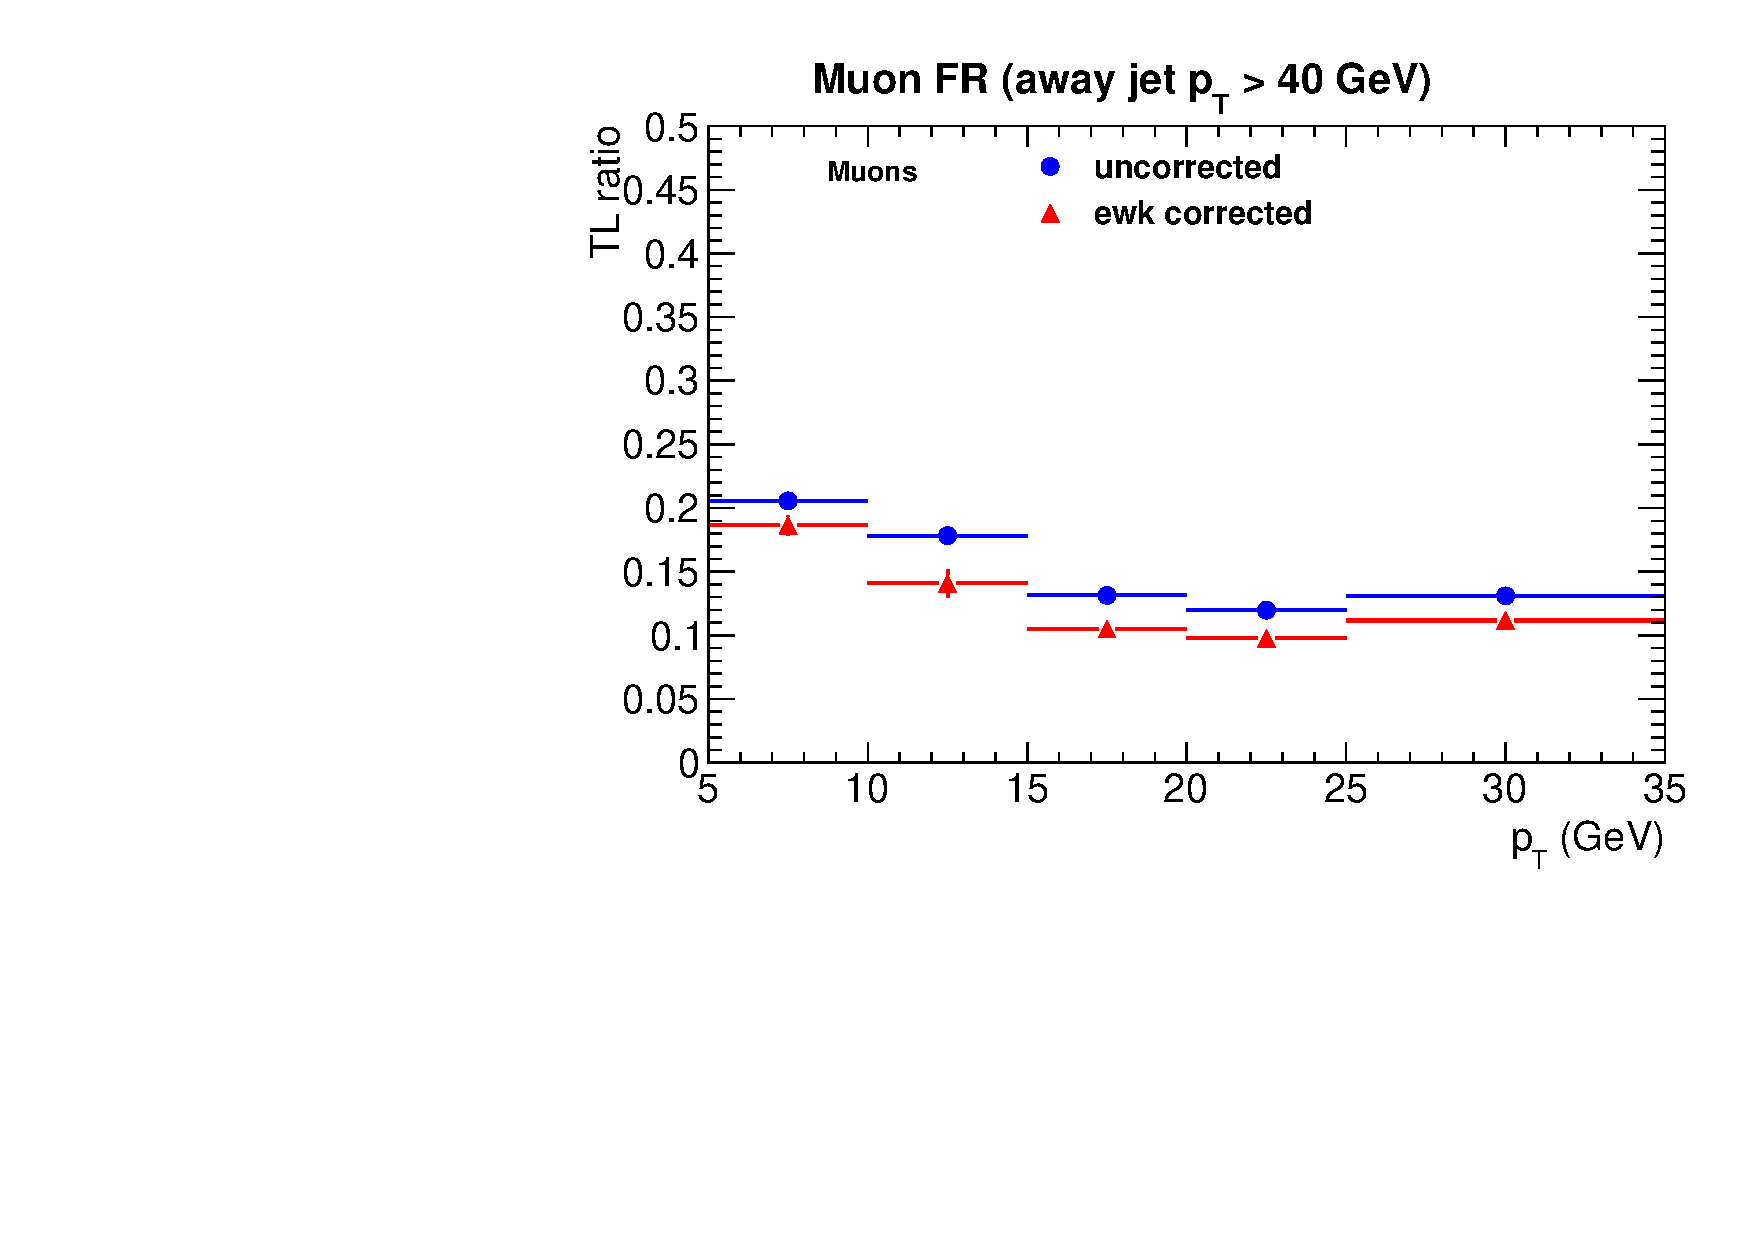
\includegraphics[width=0.48\textwidth]{p_mufr40c_vs_pt_compare_ewkcor}
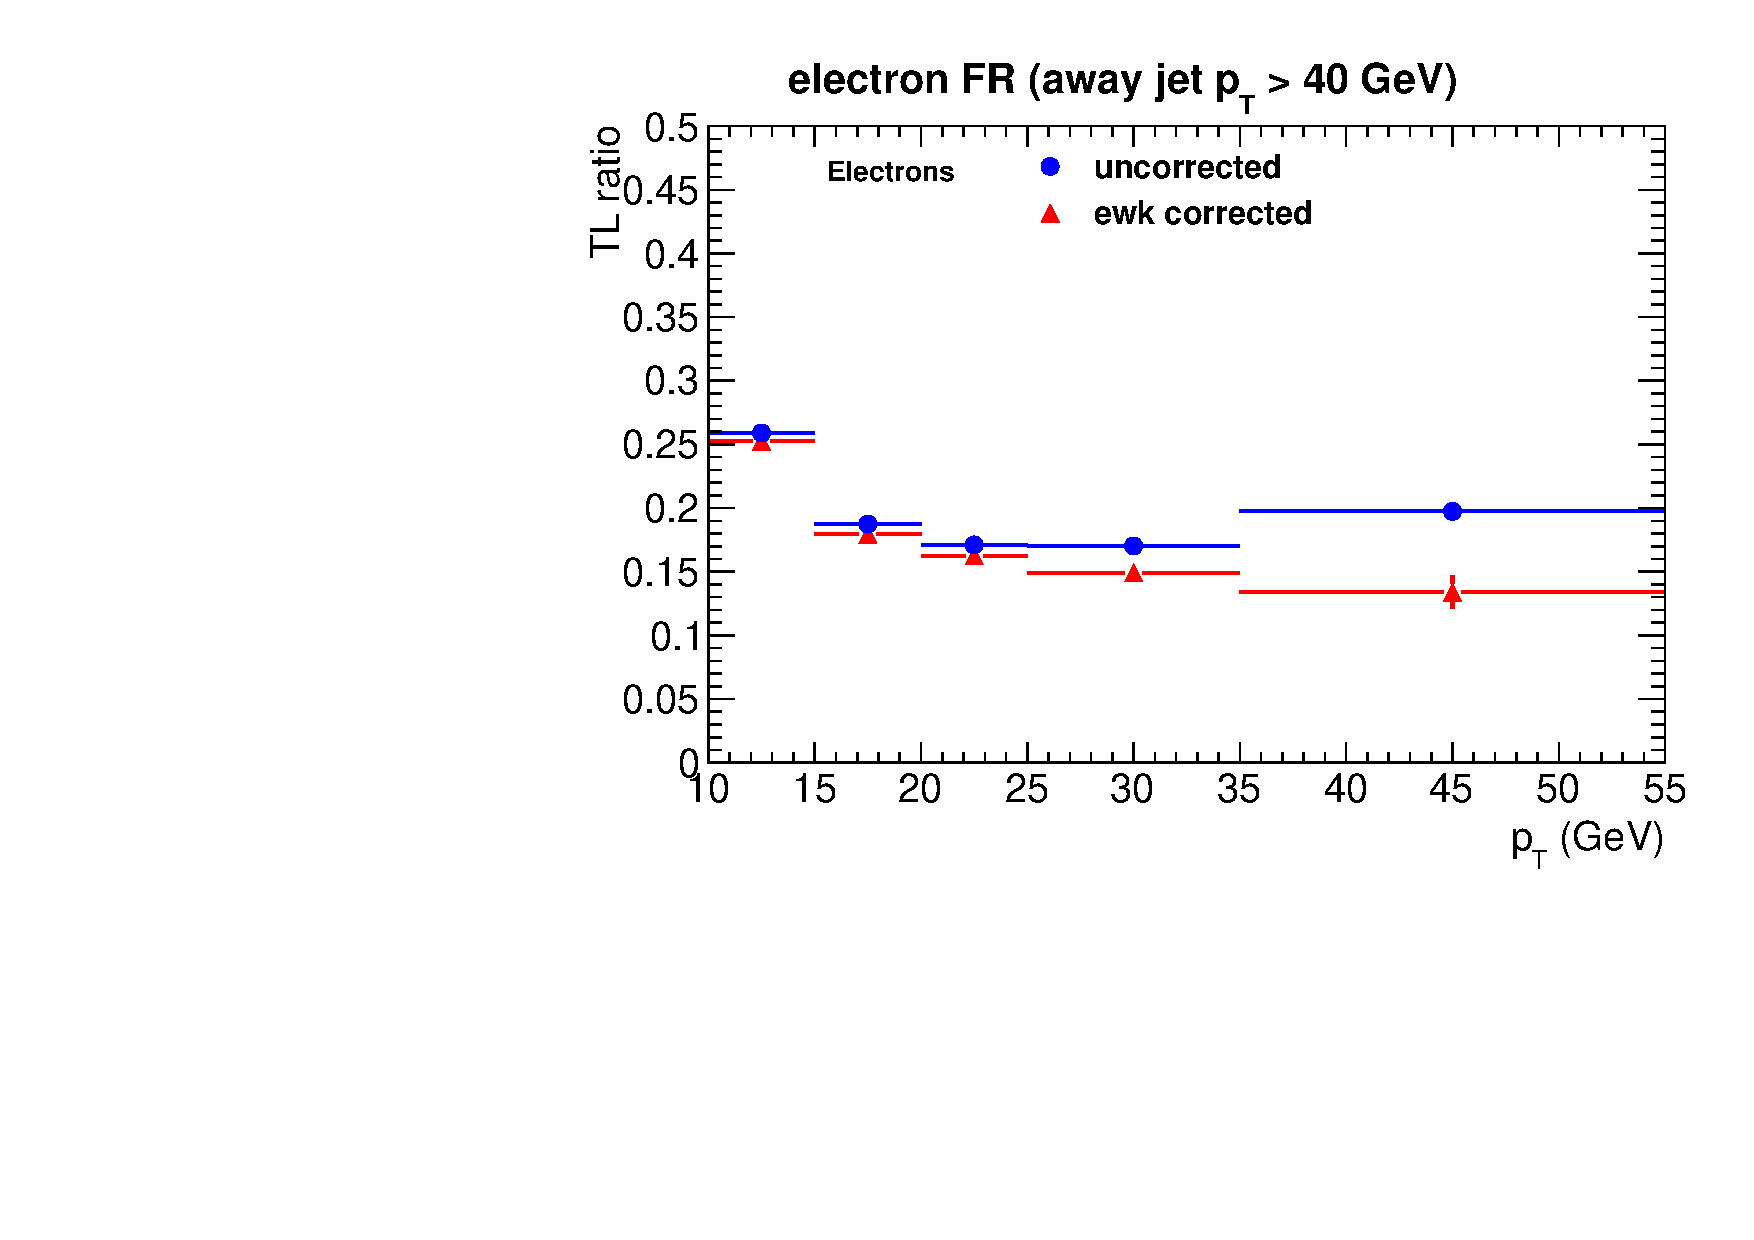
\includegraphics[width=0.48\textwidth]{p_elfr40c_vs_pt_compare_ewkcor}
\caption[The measured fake rate vs \pt before and after the electroweak corrections]
{\label{fig:bkgd_fakes_fr_mufr_ewkcont}
Projection of the muon (left) and electron (right) fake rate in data vs \pt.
The blue plot is the fake rate before the EWK correction and the red plot is
after.
}
\end{center}
\end{figure}
% --------------------------------------------------------------------------- %

% --------------------------------------------------------------------------- %
\subsection{Fake Rates for Electrons and Muons}
\label {sec:bkgd_fakes_fr}
% --------------------------------------------------------------------------- %
The fake rate is measured using the selections described
in Section~\ref{sec:bkgd_fakes_method}. As discussed in
Section~\ref{sec:bkgd_fakes_datasets}, the electron fake rates are
measured separately for the triggers with and without an online
isolation requirement. The results of the measurement for electrons are
summarized in Tables~\ref{tab:fr_elfr_hpt} and~\ref{tab:fr_elfr_lpt}.
The muon fake rates are measured using the single-muon triggers described
in Section~\ref{sec:bkgd_fakes_datasets}. The results are summarized in
Table~\ref{tab:fr_mufr}.

Figure~\ref{fig:bkgd_fakes_fr_mufr} shows the \pt, \aeta, and \nvtx projections
of the fake rate as measured in data. The fake rate is approximately flat in
\aeta. The FR decreases with increasing \pt, from a value of approximately 0.2
at 5 \GeV to about 0.13 at \hpt. The highest \pt bin shows a slight increase
in the fake rate that may be an indication that \W contamination is present,
but the increase is not significant enough to warrant considerable attentions
at this point. We assume that the fake rate is mostly constant above a $\pt >
35~\GeV$ so we assume this value in the last bin for all leptons greater than 35
\GeV.

Figure~\ref{fig:bkgd_fakes_fr_elfr} shows the \pt, \aeta, and \nvtx projections
for the electron fake rate measured with and without an online isolation
requirement. The fake rate is relatively stable, although it does show a slight
upward trend at \hpt. This is more pronounced in the fake rate with the online
isolation. Overall, the fake rate without the isolation requirement is higher
than with it, which is expected since this allows more non-prompt leptons to be
considered (due to higher denominator lepton counts). We assume that the fake
rate is mostly constant above a $\pt > 55~\GeV$ so we assume this value in the
last bin for all leptons greater than 55 \GeV.
% --------------------------------------------------------------------------- %
\begin{figure}[!hbt]
\begin{center}
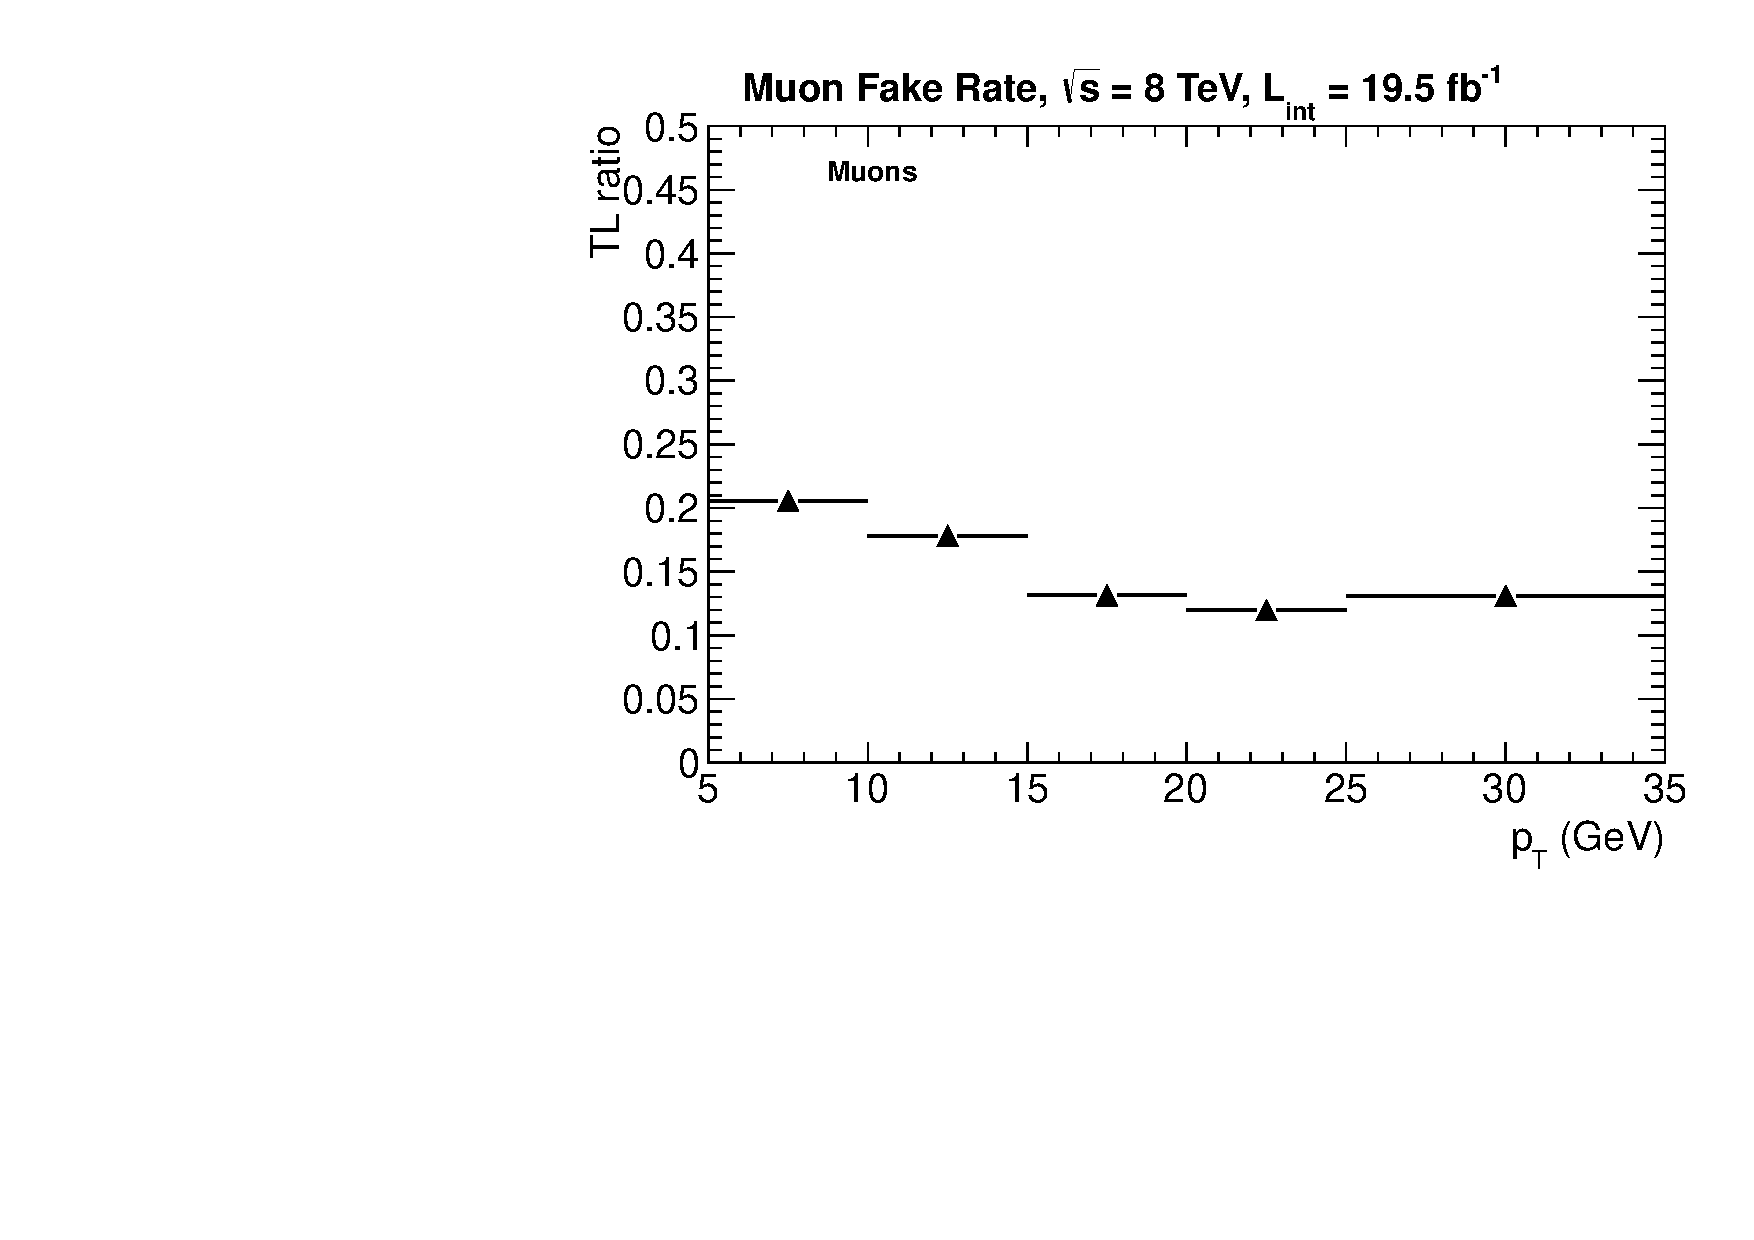
\includegraphics[width=0.48\textwidth]{p_mufr_aj40_vs_pt}
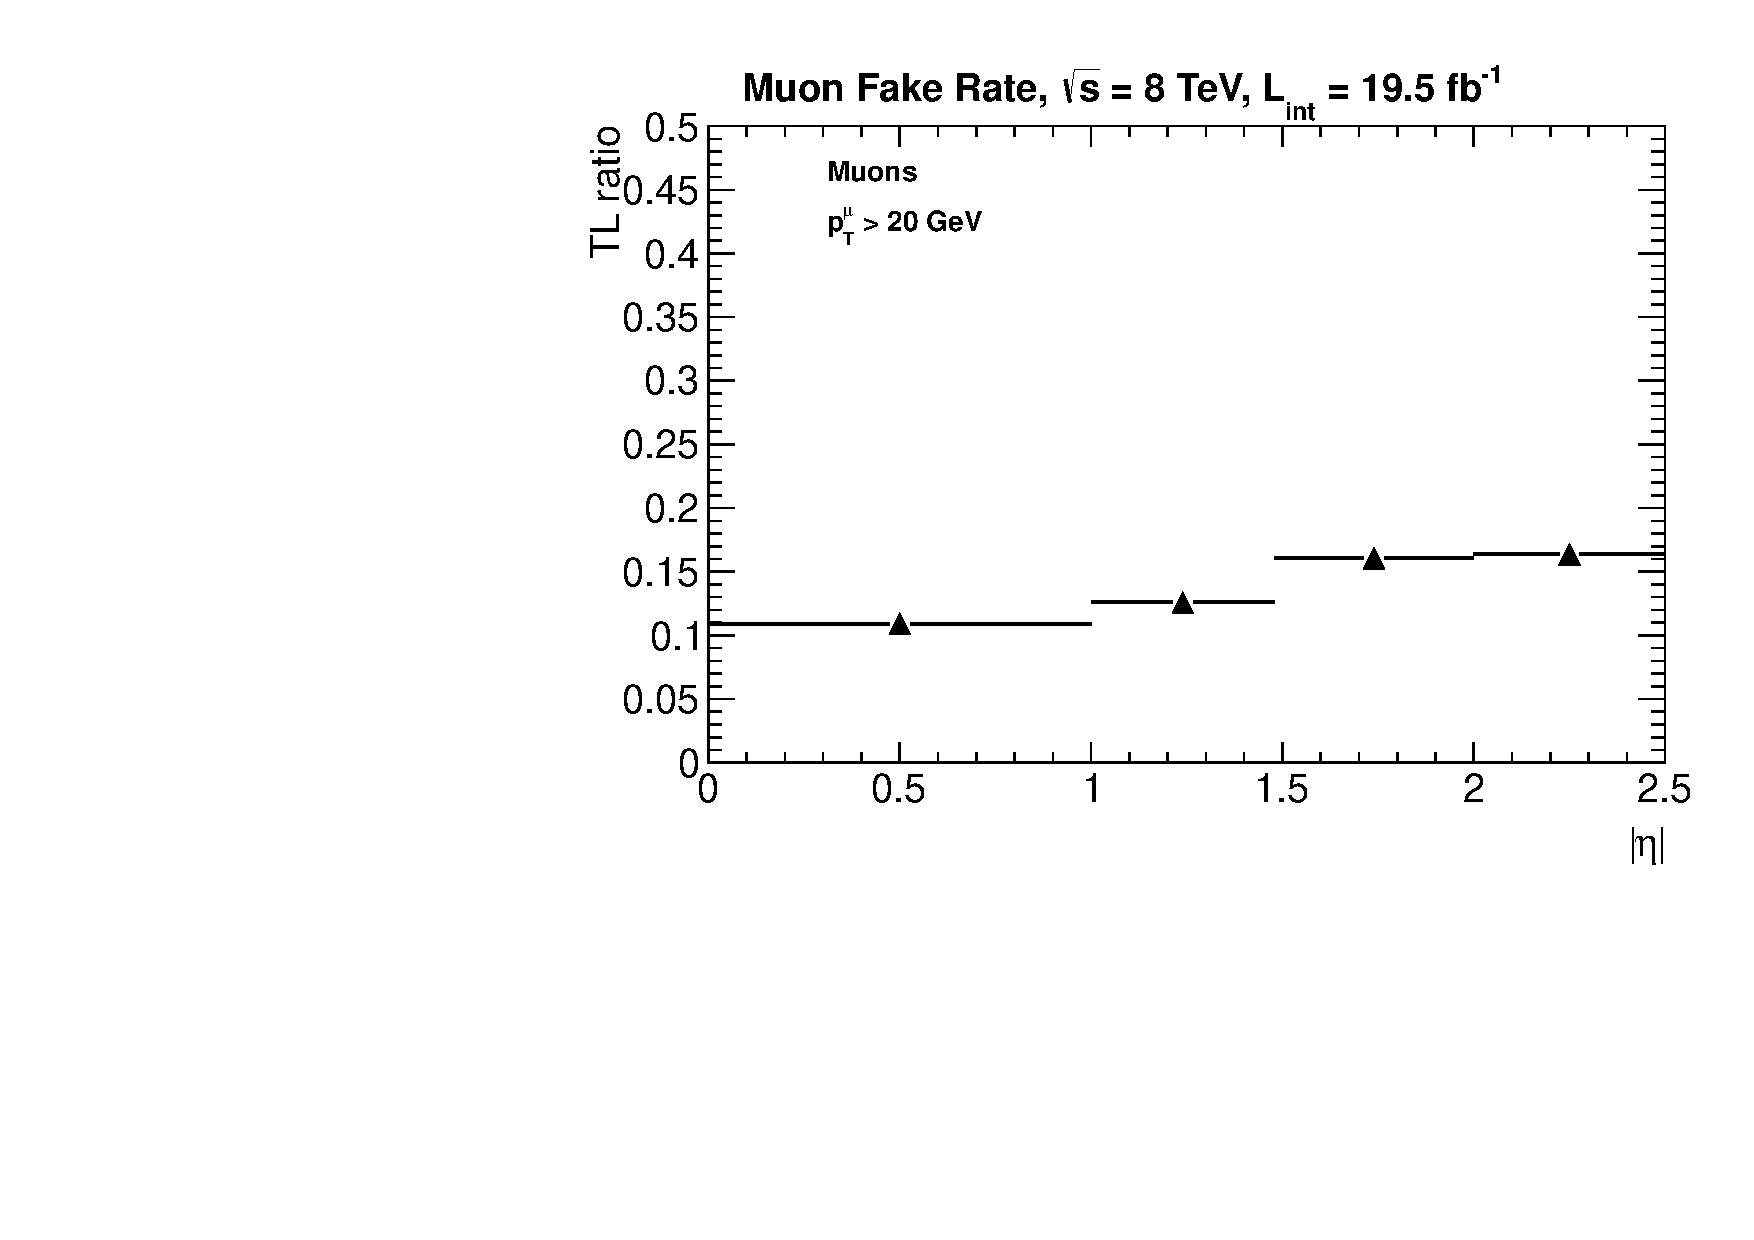
\includegraphics[width=0.48\textwidth]{p_mufr_aj40_vs_eta}
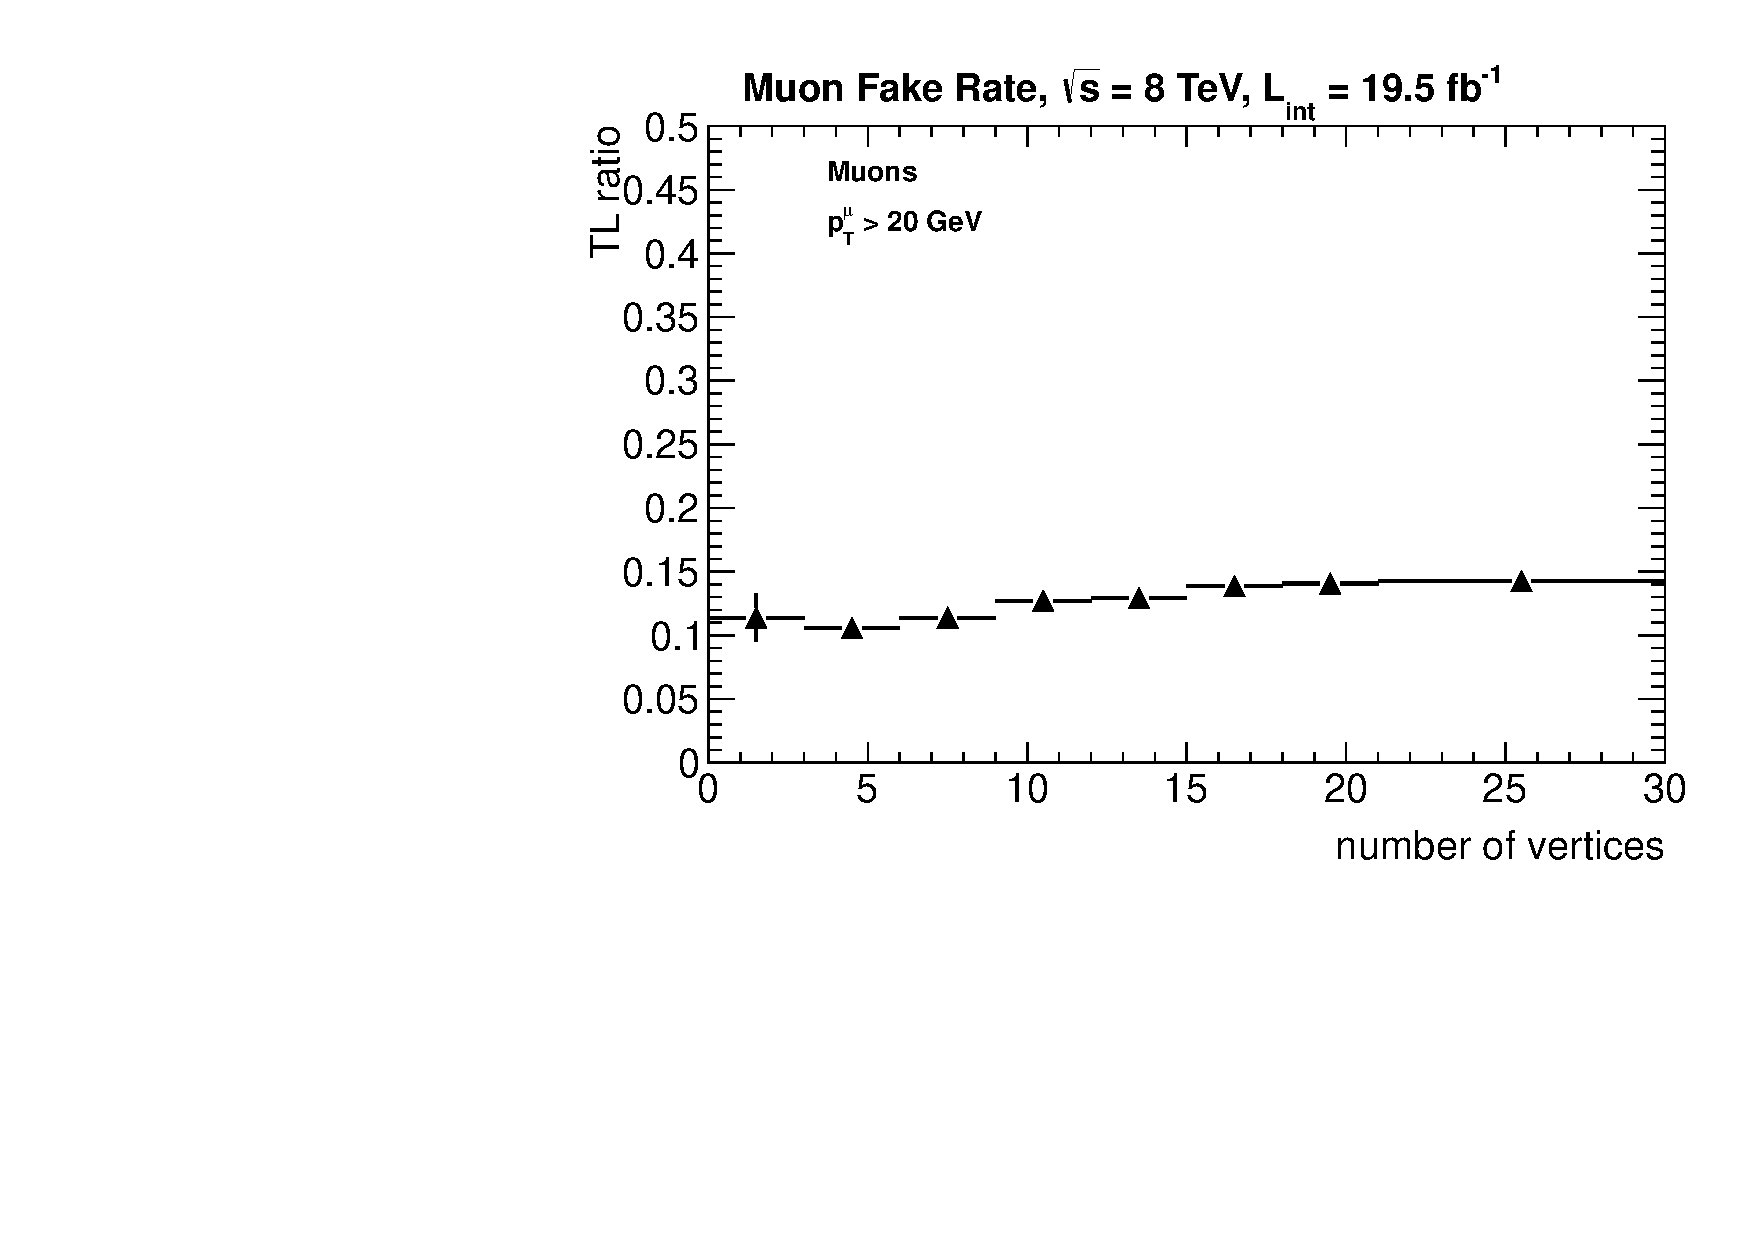
\includegraphics[width=0.48\textwidth]{p_mufr_aj40_vs_nvtxs}
\caption[Muon Fake Rate vs \pt, \aeta, and number of vertices]
{\label{fig:bkgd_fakes_fr_mufr_aj}
Projection of the muon fake rate in data vs \aeta, \pt, and the number of
vertices. This fake rate is use for both the \hpt and \lpt analysis.
}
\end{center}
\end{figure}
% --------------------------------------------------------------------------- %

% --------------------------------------------------------------------------- %
\begin{figure}[!hbt]
\begin{center}
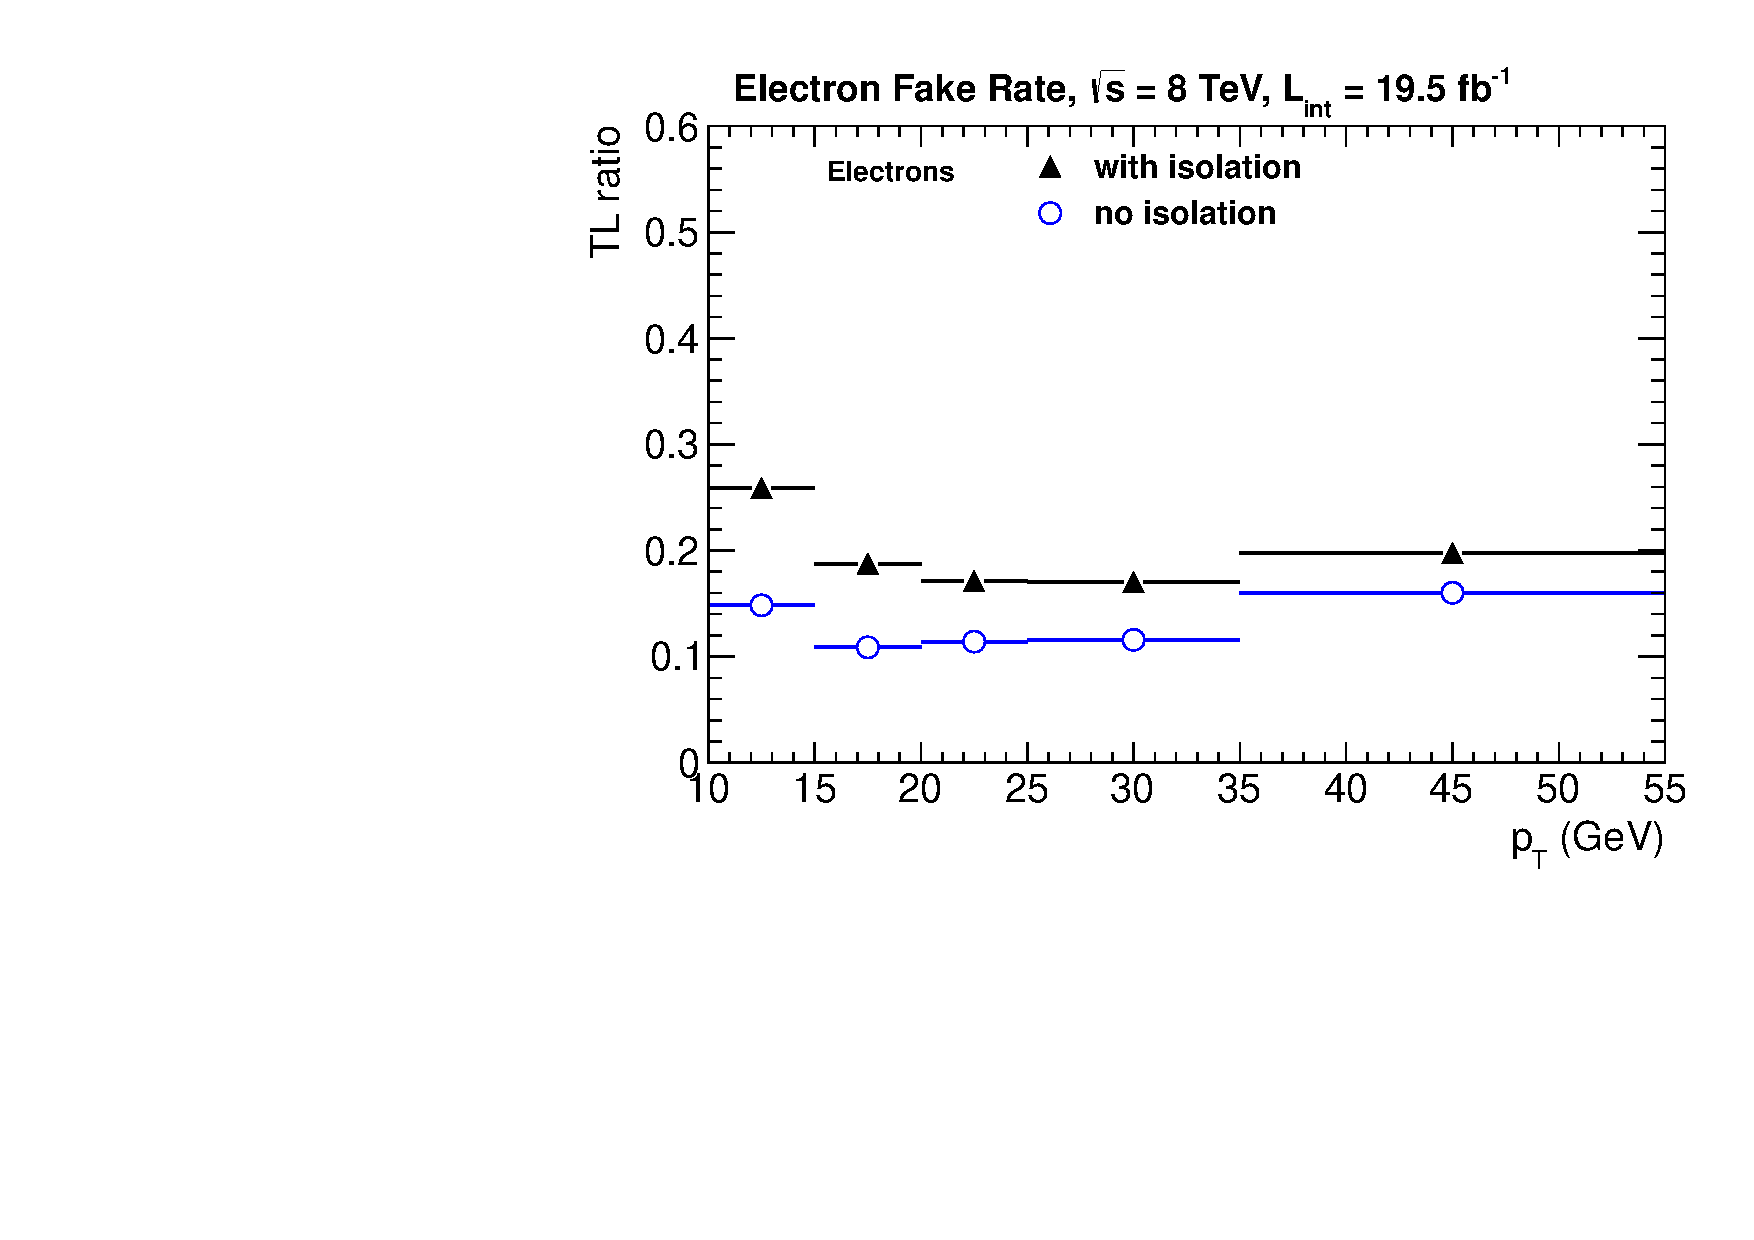
\includegraphics[width=0.48\textwidth]{p_elfr_aj40_vs_pt}
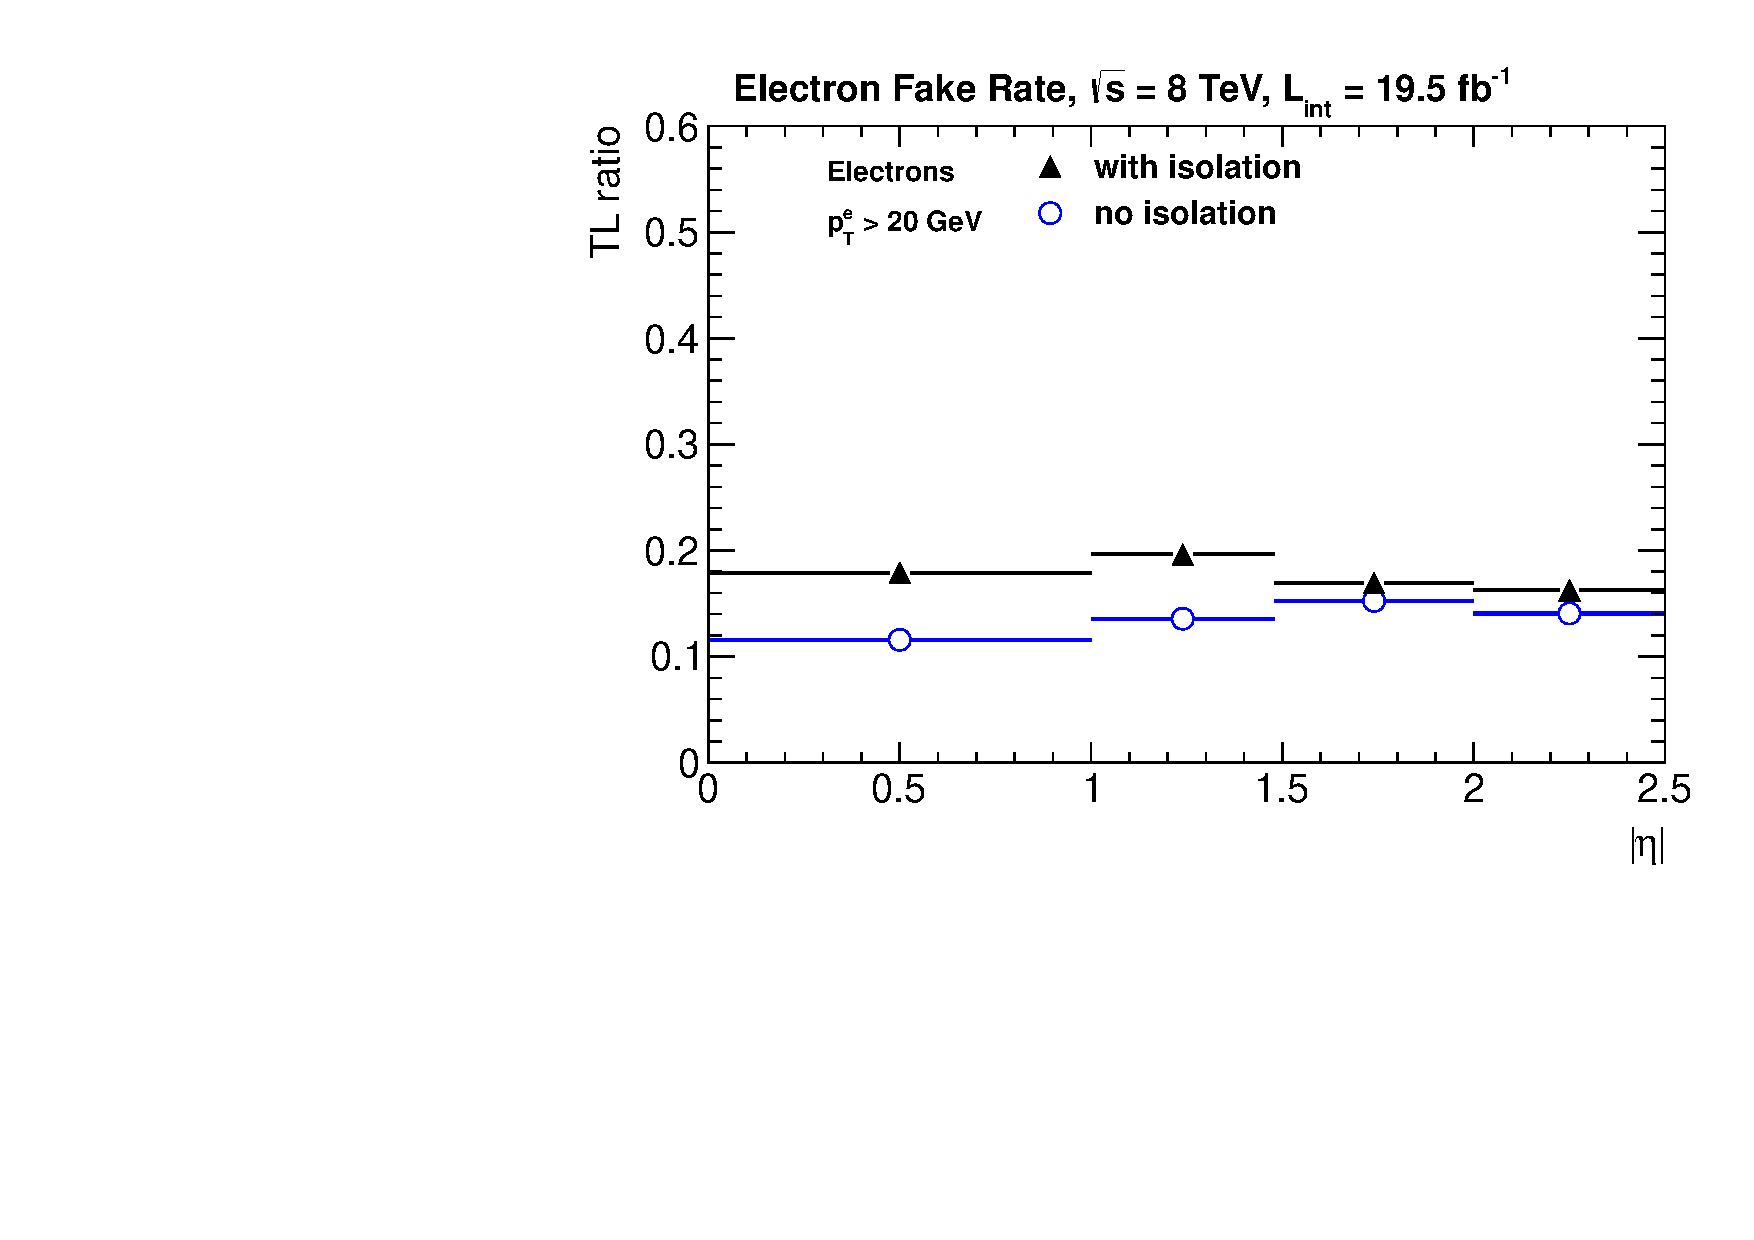
\includegraphics[width=0.48\textwidth]{p_elfr_aj40_vs_eta}
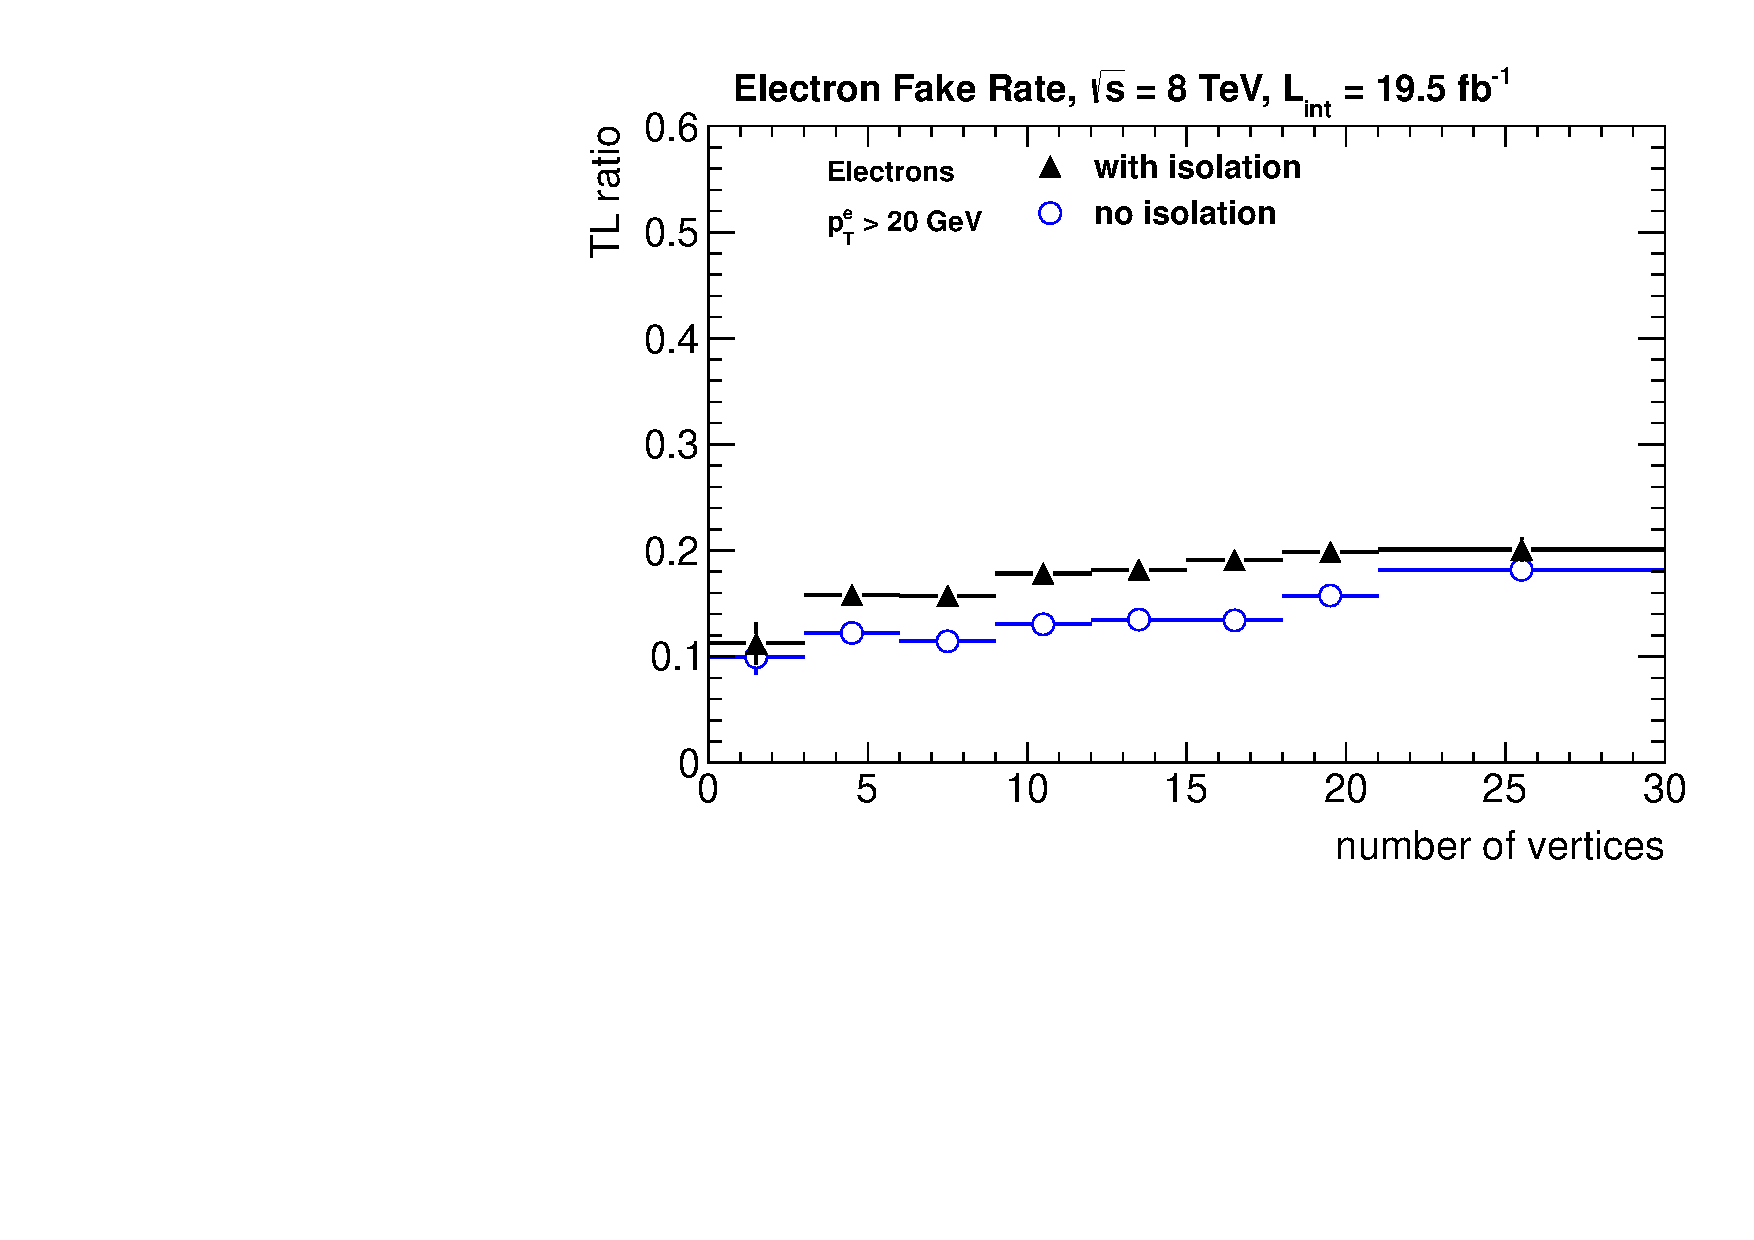
\includegraphics[width=0.48\textwidth]{p_elfr_aj40_vs_nvtxs}
\caption[Electron Fake Rate vs \pt, \aeta, and number of vertices]
{\label{fig:bkgd_fakes_fr_elfr_aj}
Projection of the electron fake rate in data vs \aeta, \pt, and the number
of vertices with (triangles) and without (open circles) an online isolation
requirement. The fake rate measured with an online isolation requirement
is used for the \hpt analysis. The triggers without the online isolation
requirement are used in the fake rate for the \lpt analysis.
}
\end{center}
\end{figure}
% --------------------------------------------------------------------------- %
% 
% --------------------------------------------------------------------------- %
\subsection{Study of Fake Rate Dependencies}
\label {sec:bkgd_fakes_frstudy}
% --------------------------------------------------------------------------- %
Several studies are performed in data and simulation to assess the dependence
of the fake rate on the kinematics. Studies of the contaminations of
the fake rate in data due to prompt leptons was already considered in
Section~\ref{sec:bkgd_fakes_lepcont}. Here we perform the following two
studies:
\begin{itemize}
\item Measurement of the fake rate dependence on the away-side jet \pt, as a
measure of the dependence of the parent parton momentum.
\item Closure test are performed using simulated QCD, \Wj, and \ttbar samples.
\end{itemize}

% --------------------------------------------------------------------------- %
\subsubsection{Fake Rate Dependence on Away Jet \pt}
\label {sec:bkgd_fakes_frstudy_aj}
% --------------------------------------------------------------------------- %
The lepton fake rates are dependent upon the away-jet requirement because
of the extrapolation in isolation. Lepton candidates in \hpt jets have a
smaller probability to pass an isolation requirement than a similar \pt lepton
candidate in a \lpt jet. The difference can be understood by considering the
relative size of the lepton \pt and the difference between the parent parton's
\pt with the lepton's \pt ($|\pt^{parton} - \pt^{lepton}|$). The latter is a
measure of the maximum transverse energy that can be deposited in the isolation
cone. Thus, for a given lepton \pt, the higher the \pt of the originating
parton, the less likely it is for this lepton to pass the numerator isolation
criteria. The probability levels off when the momentum of the parton because
much larger than that of the lepton candidate.

Figures~\ref{fig:bkgd_fakes_fr_mufr}-\ref{fig:bkgd_fakes_fr_elfr_noiso} show
the \aeta and \pt projections for the muon and electron fake rates measured in
the data with \pt $>20$, 40, and 60 \GeV away-jet requirements. The range of
jet \pt considered was determined by looking at the typical \pt spectrum of
\bqs with FO daughters in simulated \ttbar events. The dependence of the muon
fake rate on the away-jet \pt requirement is $\sim 30\%$. The dependence is
flat in \aeta, but increases with \pt for the muon candidate. The dependence of
the electron fake rates on the away-jet \pt is similarly $\sim 30\%$. There is
not a strong trend in either \aeta or \pt. The dependence appears similar for
electron fake rates measured with and without an isolation requirement.

% --------------------------------------------------------------------------- %
\begin{figure}[!hbt]
\begin{center}
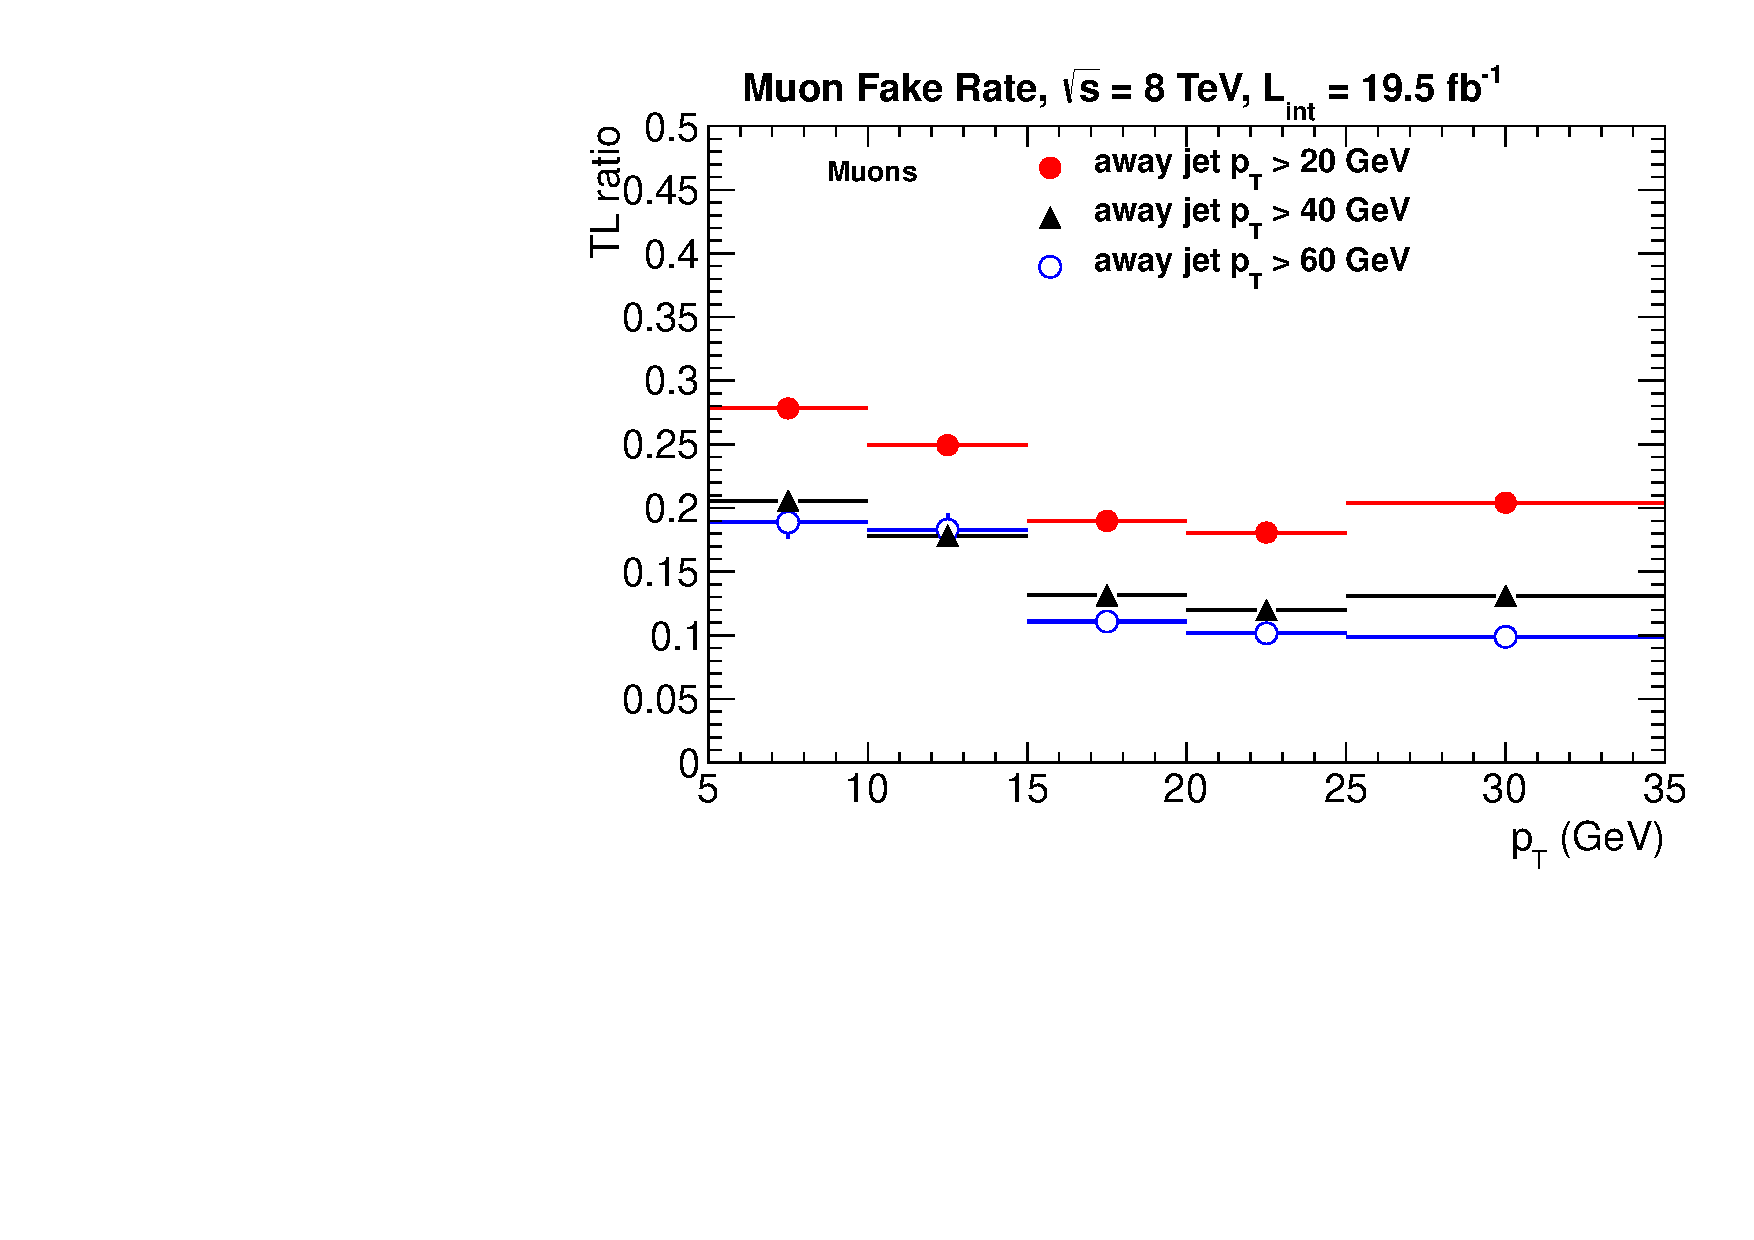
\includegraphics[width=0.48\textwidth]{p_mufr_vs_pt}
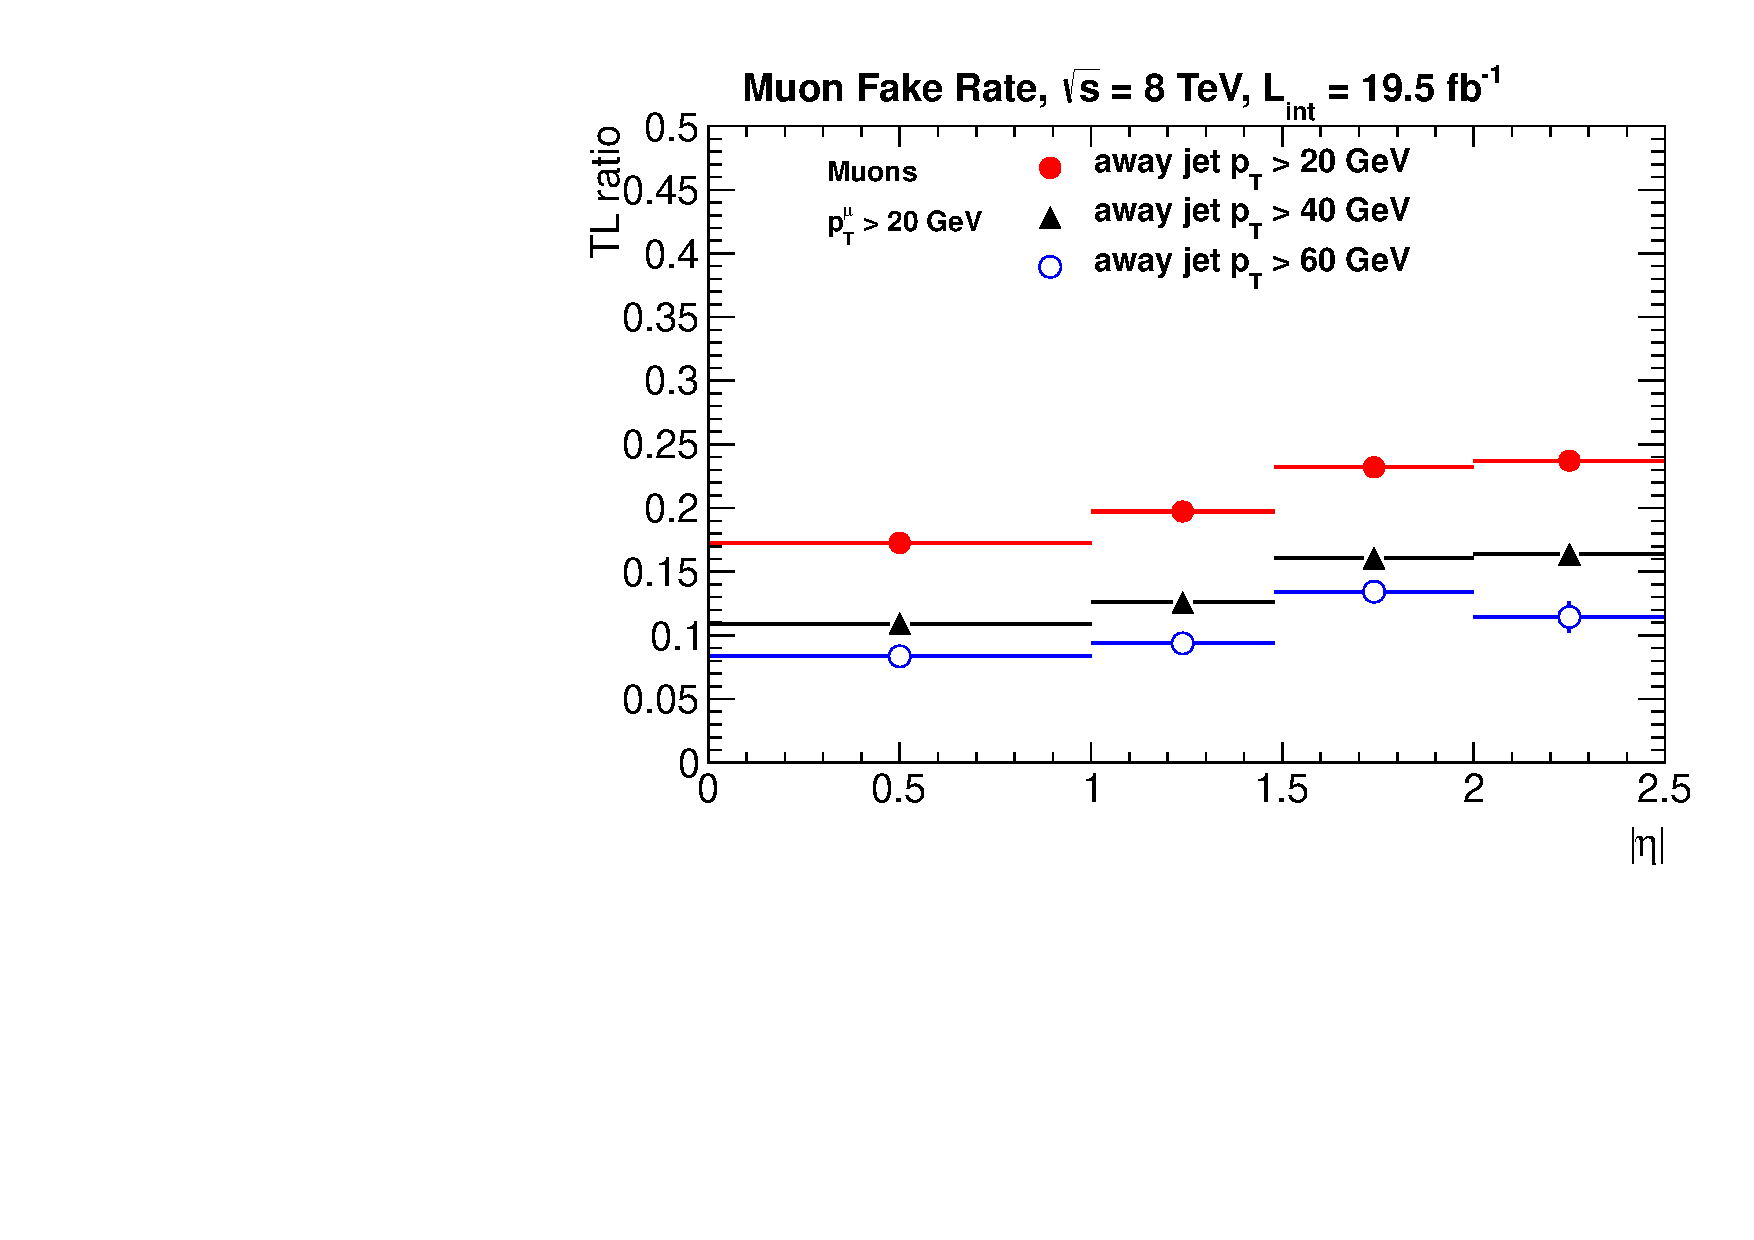
\includegraphics[width=0.48\textwidth]{p_mufr_vs_eta}
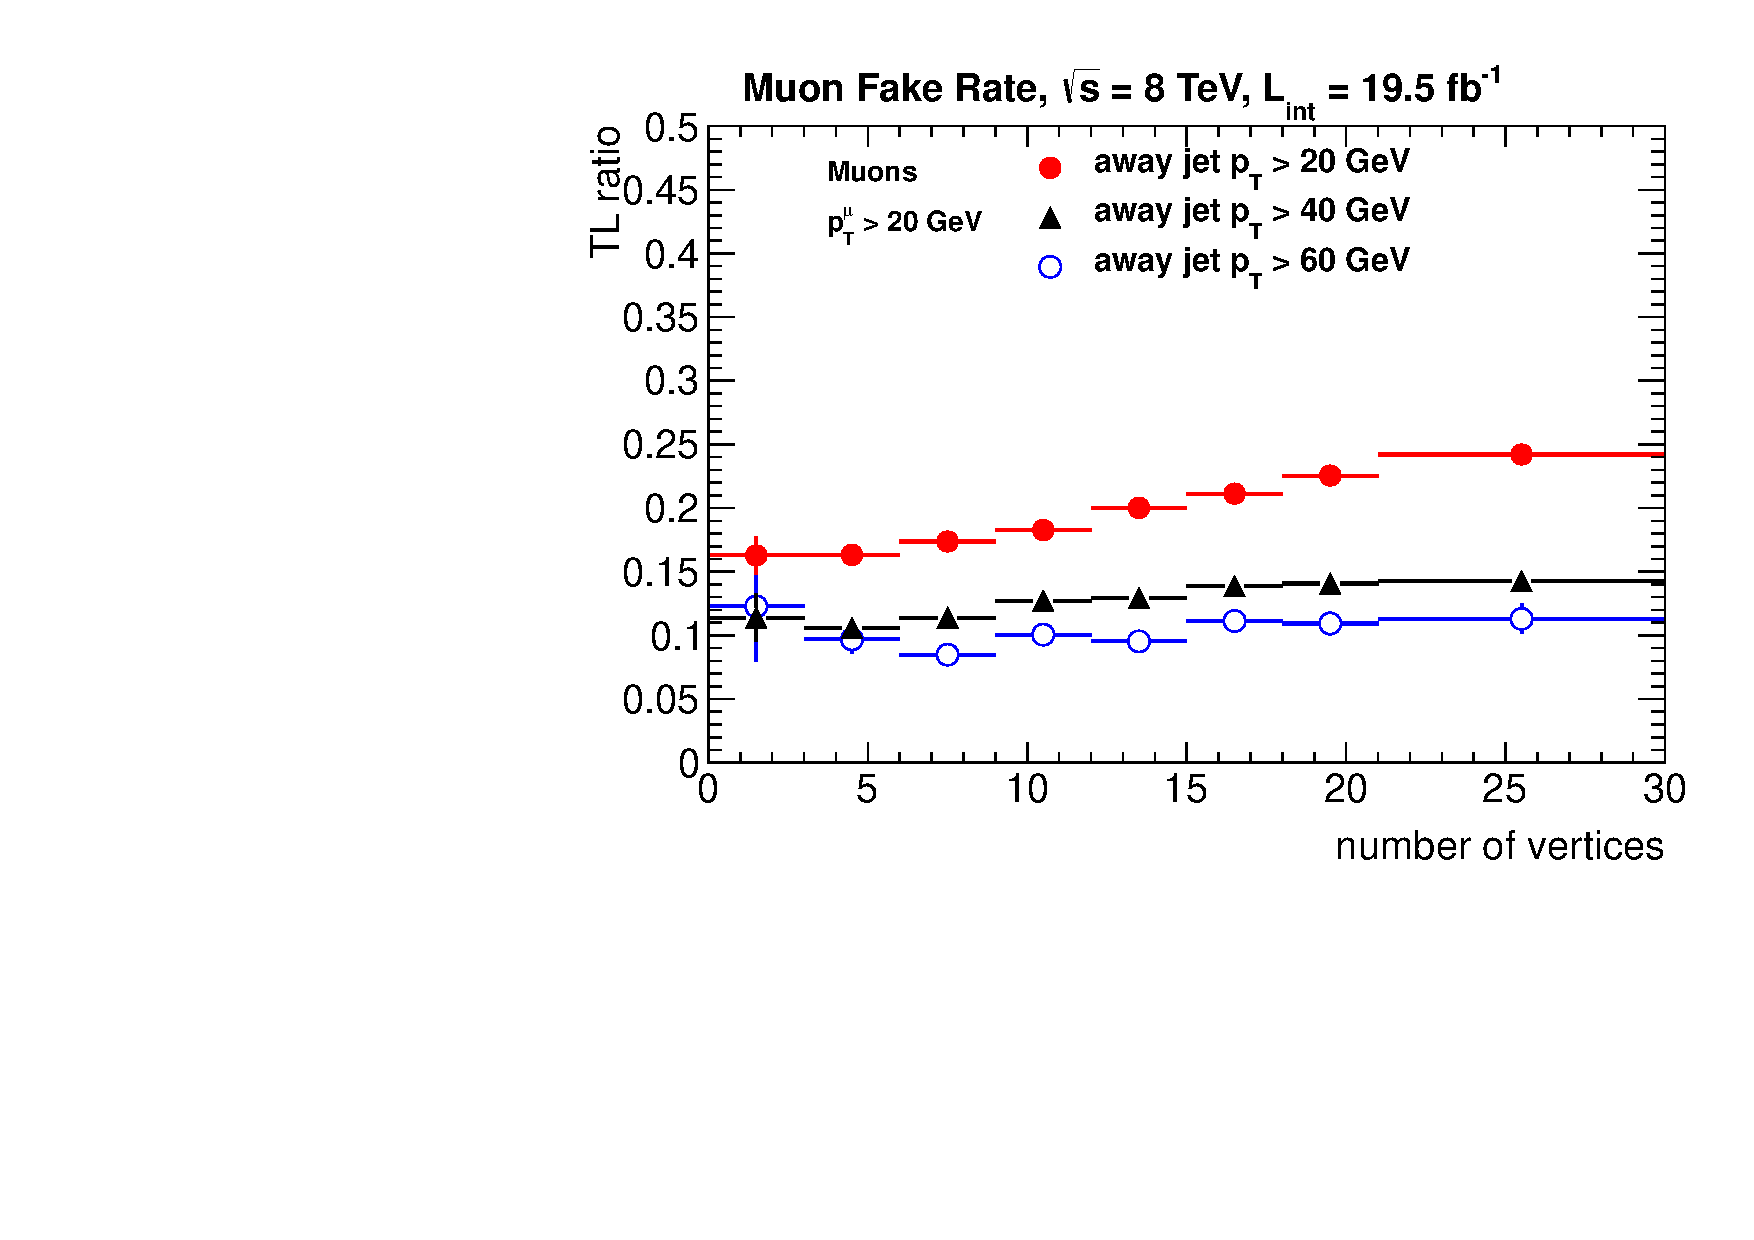
\includegraphics[width=0.48\textwidth]{p_mufr_vs_nvtxs}
\caption[Muon Fake Rate vs \pt, \aeta, and number of vertices for different away jet \pt requirements]
{\label{fig:bkgd_fakes_fr_mufr}
Projection of the muon fake rate in data vs \aeta, \pt, and \nvtx for different
away jet \pt requirements. The away jet is a corrected particle flow jet and is
required to be $\DR > 0.1$ away from the muon candidate.
}
\end{center}
\end{figure}
% --------------------------------------------------------------------------- %

% --------------------------------------------------------------------------- %
\begin{figure}[!hbt]
\begin{center}
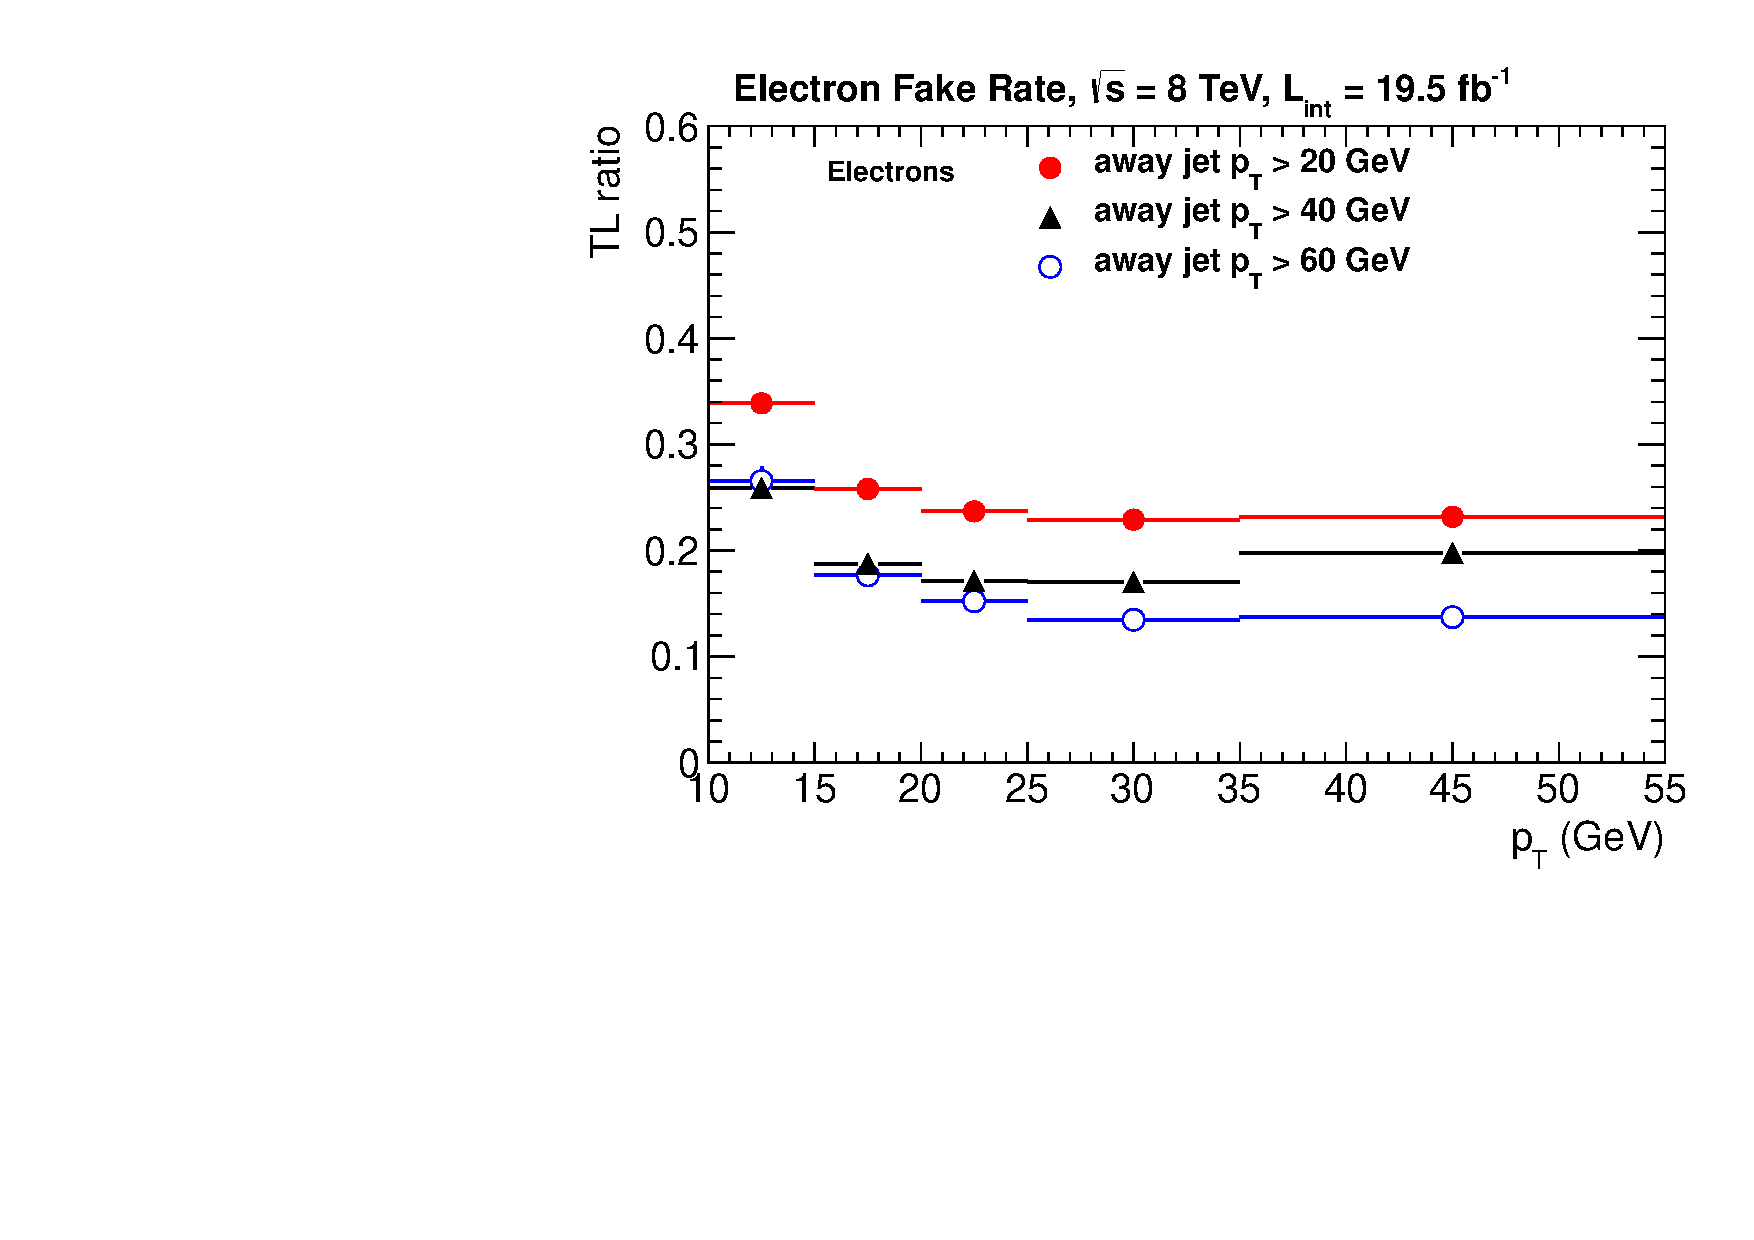
\includegraphics[width=0.48\textwidth]{p_elfr_vs_pt}
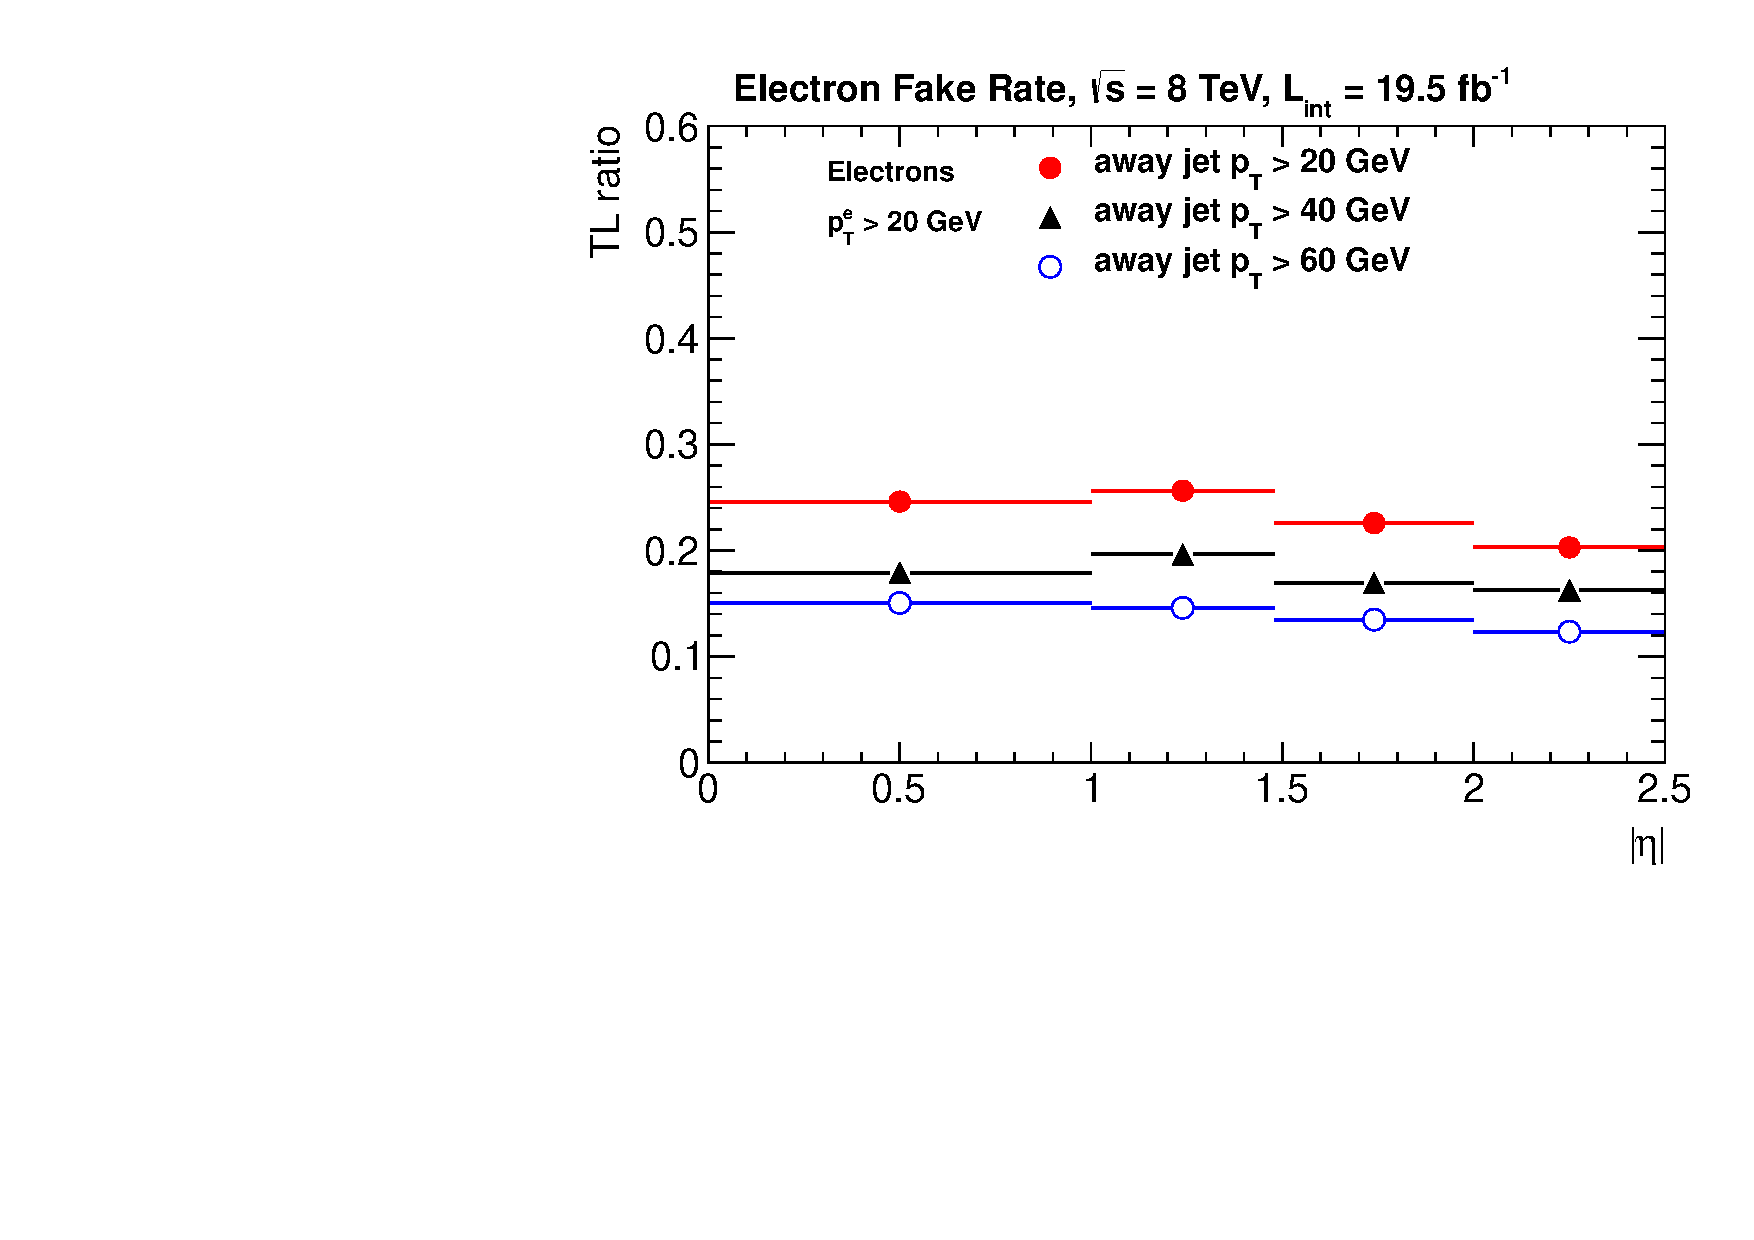
\includegraphics[width=0.48\textwidth]{p_elfr_vs_eta}
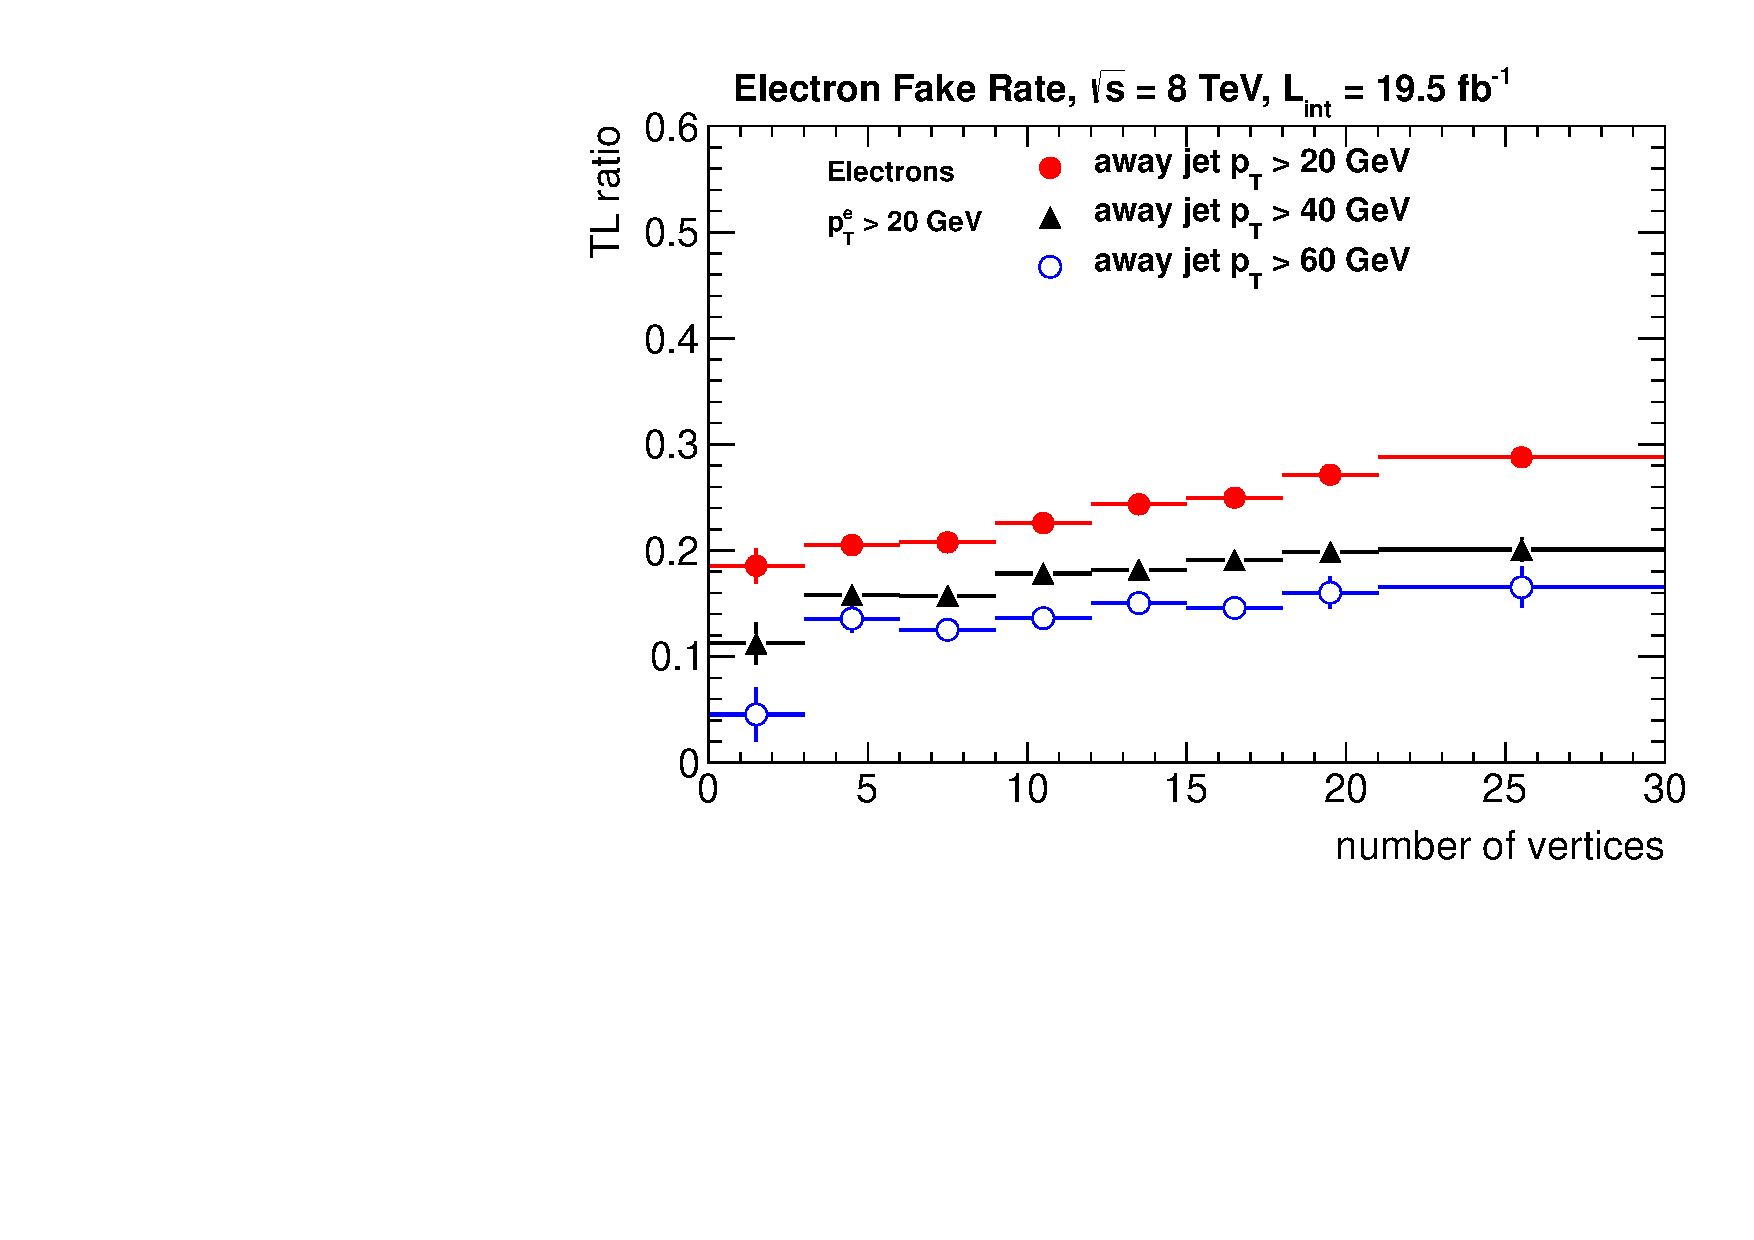
\includegraphics[width=0.48\textwidth]{p_elfr_vs_nvtxs}
\caption[Electron Fake Rate vs \pt, \aeta, and number of vertices for different away jet \pt requirements (with online isolation requirement)]
{\label{fig:bkgd_fakes_fr_elfr}
Projection of the electron fake rate in data vs \aeta, \pt, and \nvtx for
different away jet \pt requirements. The away jet is a corrected particle
flow jet and is required to be $\DR > 0.1$ away from the electron candidate.
The electron fake rate is measured using triggers with an online isolation
requirement.
}
\end{center}
\end{figure}
% --------------------------------------------------------------------------- %

% --------------------------------------------------------------------------- %
\begin{figure}[!hbt]
\begin{center}
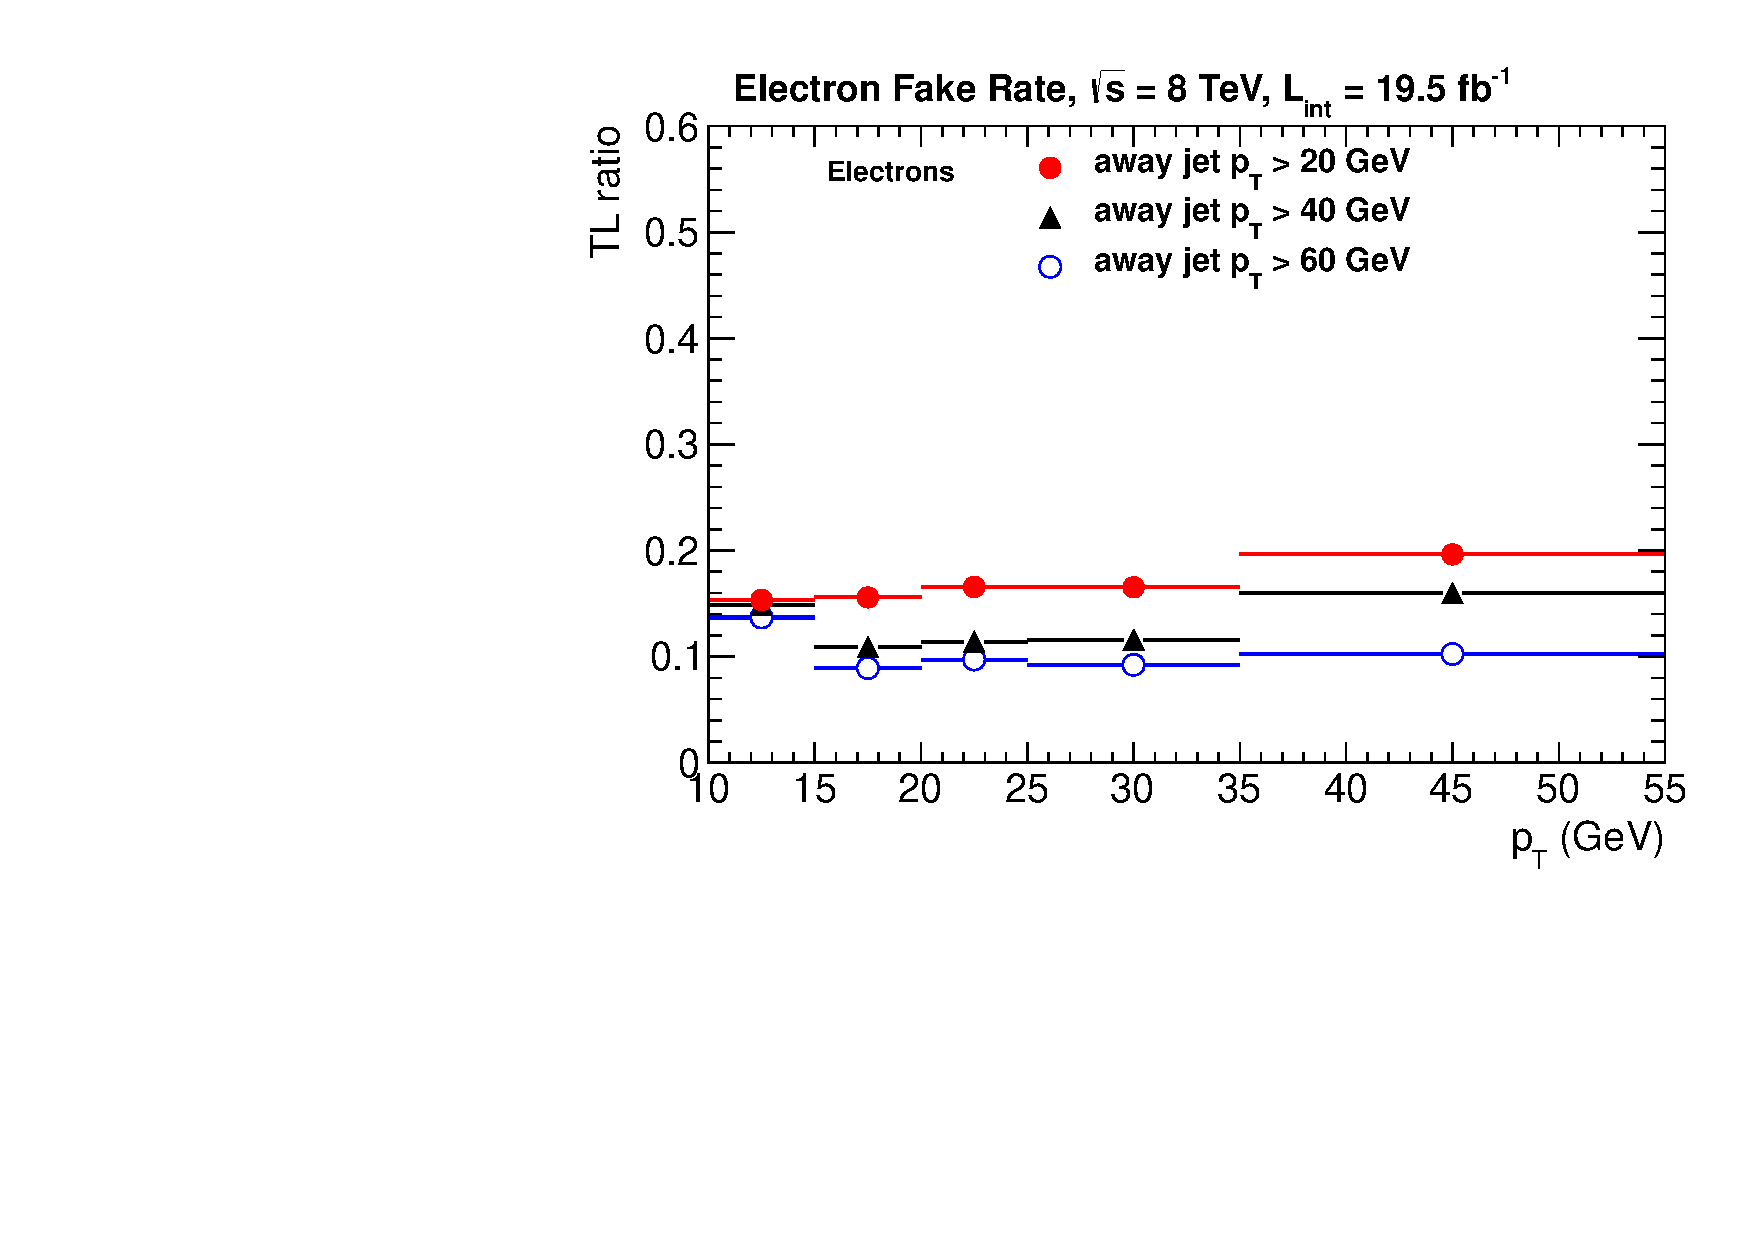
\includegraphics[width=0.48\textwidth]{p_elfr_trig_noiso_vs_pt}
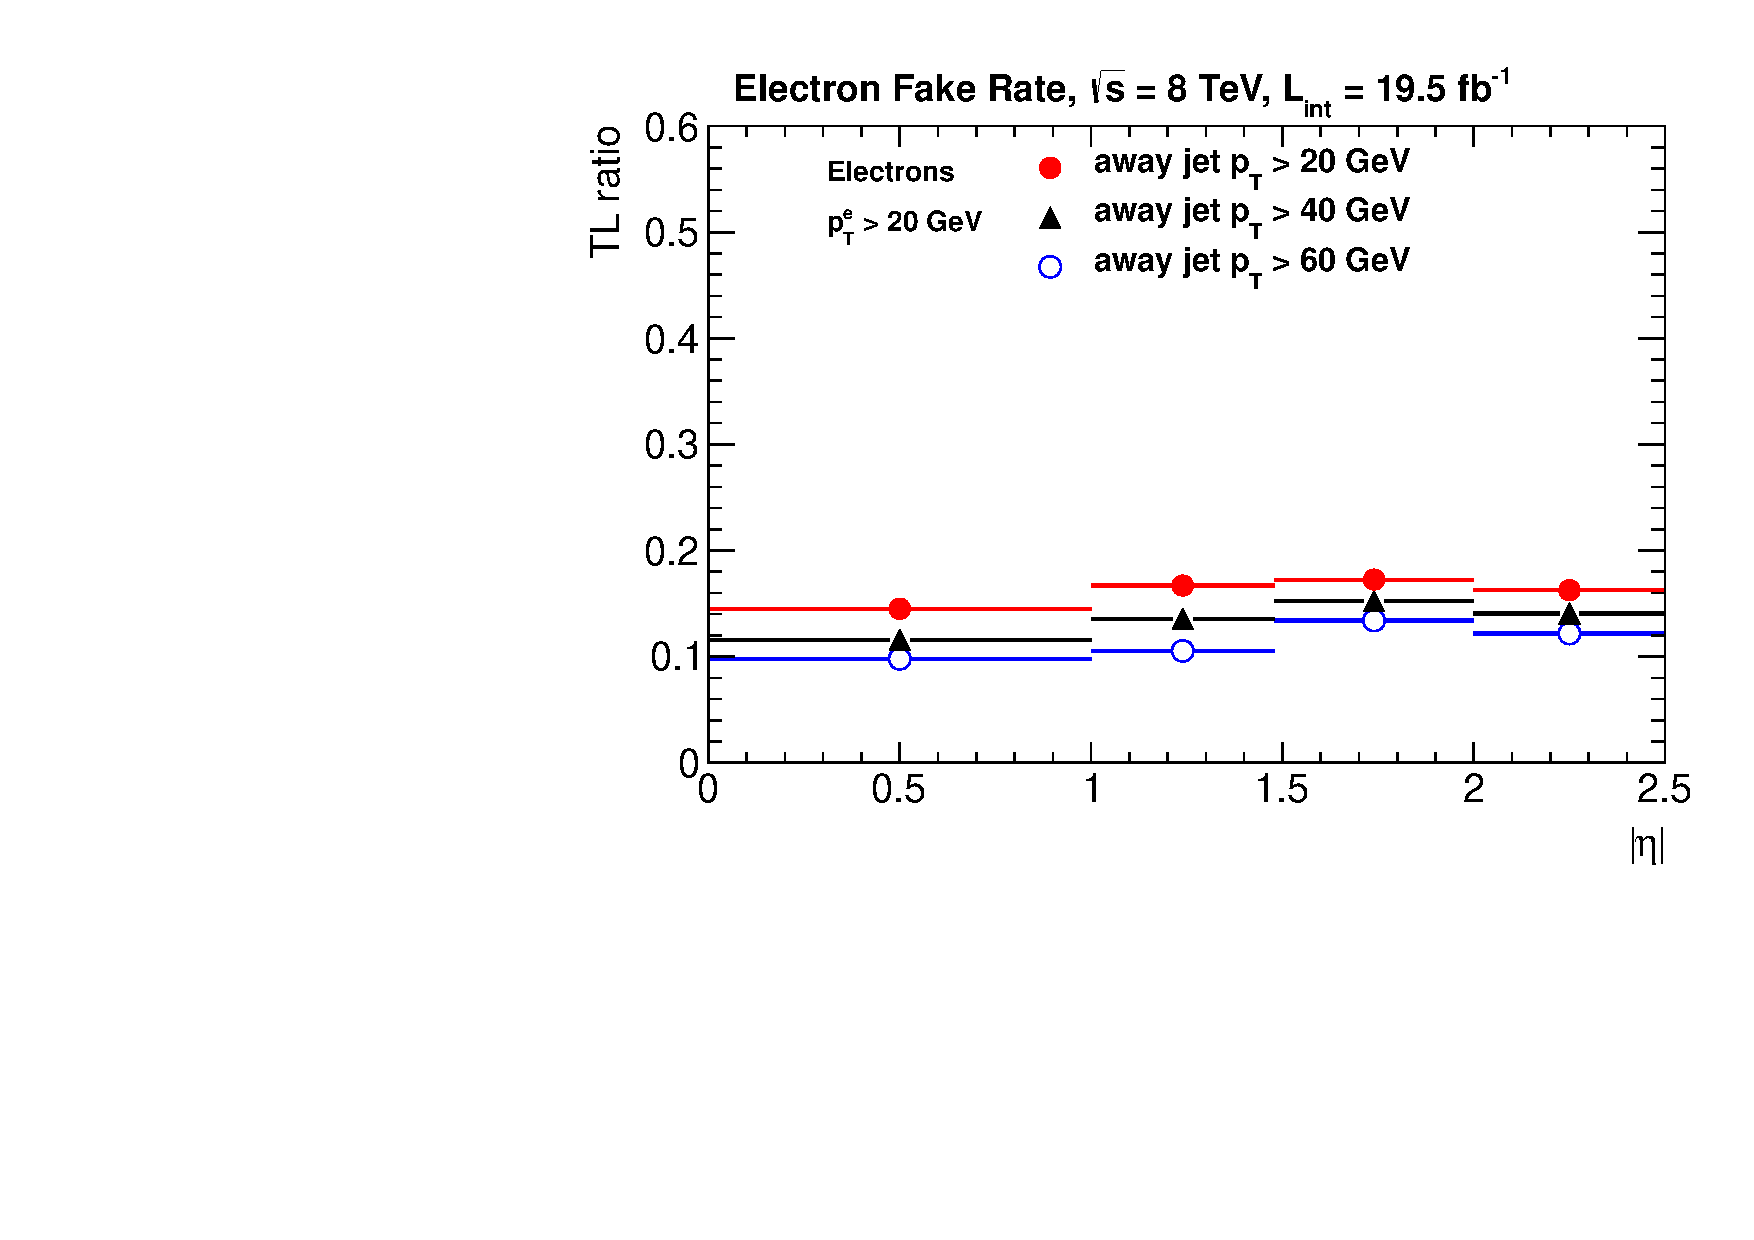
\includegraphics[width=0.48\textwidth]{p_elfr_trig_noiso_vs_eta}
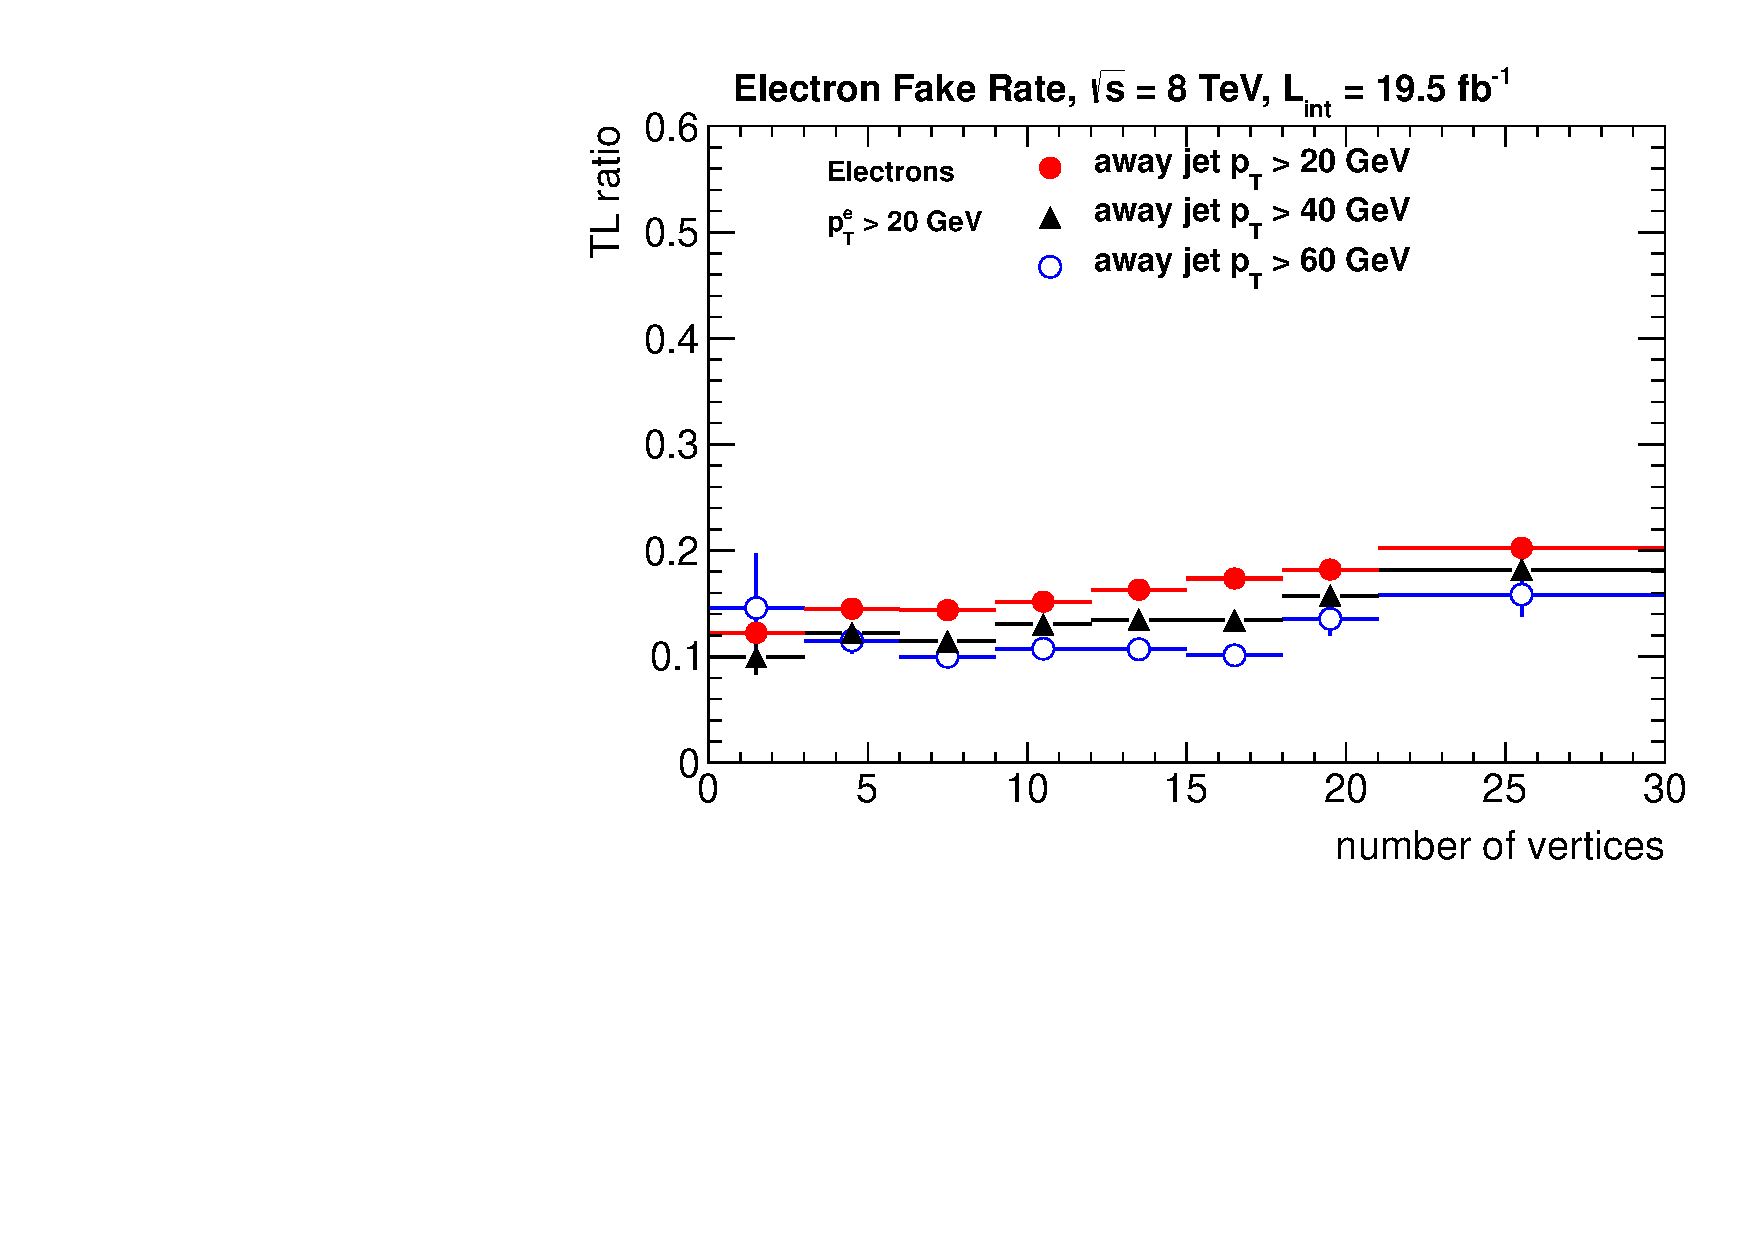
\includegraphics[width=0.48\textwidth]{p_elfr_trig_noiso_vs_nvtxs}
\caption[Electron Fake Rate vs \pt, \aeta, and number of vertices for different away jet \pt requirements (no online isolation requirement)]
{\label{fig:bkgd_fakes_fr_elfr_noiso}
Projection of the electron fake rate in data vs \aeta, \pt, and \nvtx for
different away jet \pt requirements. The away jet is a corrected particle
flow jet and is required to be $\DR > 0.1$ away from the electron candidate.
The electron fake rate is measured using triggers without an online isolation
requirement.
}
\end{center}
\end{figure}
% --------------------------------------------------------------------------- %

% --------------------------------------------------------------------------- %
\subsubsection{Fake Rate Closure Tests}
\label {sec:bkgd_fakes_frstudy_closure}
% --------------------------------------------------------------------------- %

We test that the fake rates measured in QCD are applicable to the dilepton
samples by performing a closure test on a simulated \ttbar and \Wj sample. The
closure test uses QCD MC to derive the fake rate itself and applied events
selected from \ttbar and \Wj MC sample. See Table~\ref{tab:bkgd_fakes_mc}
for the MC samples used for this test. Other dilepton processes with fakes,
such as QCD with two fakes, are expected to contribute negligibly to the events
selected in this analysis. First we describe the results of the closure test
using \ttbar and \Wj events with the QCD derived fake rate. The following selections
are applied to events entering the \ttbar and \Wj closure tests:
% --------------------------------------------------------------------------- %
\begin{enumerate}
\item Select events that pass the baseline selections (SR0, SR10, SR20). For
\Wj, the statistics was too low so only the SR0 is considered.
\item Require at truth level that for \ttbar events, the top-quark pairs decay
semi-leptonically (i.e. one $\Wlnu$ and the other $\Wqq$).
\item Require that one lepton (real) is matched to the leptonic W decay and
the other (fake) lepton is not matched to the leptonic W decay and passes the
denominator but {\bf not} the full lepton selections.  This is the FO count.
\item Scale the FO count by $\epsilon_{FR}/(1-\epsilon_{FR})$ where
$\epsilon_{FR}$ is the QCD MC derived fake rate as a function of the fake
lepton \pt~and \aeta\ -- this is the prediction of the number of fakes passing
the full lepton selections.
\item Require that one lepton (real) is matched to the leptonic W decay and the
other (fake) lepton is not matched to the leptonic W decay and passes the full
lepton selections -- this is the observed number of fake events.
\item Compare the predicted and observed number of fake events.
\end{enumerate}
% --------------------------------------------------------------------------- %
% The number of events with fake leptons in \ttbar events is consistently
% overestimated for both electrons and muons by as much as 70\%. The observations
% are consistent with studies performed during previous version of this analysis
% ~\cite{an_ss2011,an_ssb2011}.

Table~\ref{tab:bkgd_fakes_closure} shows the results of the closure test.
As in past iterations of this analysis, there is an over-prediction in
the \ttbar~MC~\cite{sspaper2010,sspaper2011}. The systematic uncertainty
of $\pm50\%$ per fake lepton is estimated for the fake rate method. Our
understanding of the these results is that the main underlying cause
is the dependence of the fake rate on the parent parton momentum. The
momentum spectrum of partons from ISR/FSR differs from that of the b-jets
or light-flavor-quark jets (\Wqq) arising from $t\to W b$ decays. The
mix of the spectra varies, but the range of the fake rate variation can
be tested in data QCD used to measure the fake rate by applying varying
threshold to the away jet as illustrated in Fig.~\ref{fig:bkgd_fakes_fr_mufr}
and~\ref{fig:bkgd_fakes_fr_elfr_noiso}.

We compute the contributions from double-fake and single-fake events separately
and based on the results of the closure test, we assign a 50\% systematic
uncertainty on the combined estimate.

% --------------------------------------------------------------------------- %
\subsubsection{Contamination from Signal Events}
\label {sec:bkgd_fakes_sc}
% --------------------------------------------------------------------------- %

Signal contamination enters when there is a significant source of two ``real''
leptons, with one or both failing the numerator selections, but passing the
denominator cuts and comprising a significant fraction of the total number of
single fake or double fake counts. An additional simulation based correction
is applied where simulated truth information is used to select events with
two real same-sign dileptons failing the numerator selections but passing the
denominator selection. These datasets correspond to the rare SM samples discussed
in Section~\ref{sec:ss_rare}. These events are weighted using the same fake rate
as we apply to data and then subtracted from the data driven prediction for
fake events. This corrected fake prediction is then used in the analysis.

% --------------------------------------------------------------------------- %
\begin{table}[!htb]
\begin{center}
\caption[Fake rate closure tests on \ttbar and \Wj events from simulation applied to a fake derived from QCD simulation]
{\label{tab:bkgd_fakes_closure}
Fake rate closure tests on \ttbar and \Wj events from simulation applied to a
fake derived from QCD simulation. The \ttbar closure test shows results for
the baseline search regions with exactly zero, exactly one and at least two
\bjs (SR0, SR10, SR20). Due to limited statistics, the \Wj closure test is only
performed on the baseline search region with a \bj veto applied (SR0).
``p'' and ``o'' refer to the predicted and the observed counts, respectively.
}
\end{center}
\resizebox{0.8\textwidth}{!}{\begin{minipage}{\textwidth}
\begin{tabular}{l|c|l|cccc}
\hline\hline
Sample                   & search region         & result   & \ee                 & \mm                & \em                  & $\ll$                \\ \hline
\multirow{12}{*}{\ttbar} & \multirow{4}{*}{SR0}  & pred     & 756.8 $\pm$ 194.8   & 830.9 $\pm$ 13.0   & 1592.7 $\pm$ 230.0   & 3180.5 $\pm$ 301.6   \\
                         &                       & obs      & 339                 & 318                & 656                  & 1313                 \\
                         &                       & pred/obs & 2.23 $\pm$ 0.59     & 2.61 $\pm$ 0.15    & 2.43 $\pm$ 0.36      & 2.42 $\pm$ 0.24      \\
                         &                       & (p-o)/p  & 0.55 $\pm$ 0.12     & 0.62 $\pm$ 0.02    & 0.59 $\pm$ 0.06      & 0.59 $\pm$ 0.04      \\ \cline{2-7}
                         & \multirow{4}{*}{SR10} & pred     & 381.3  $\pm$ 99.1   & 420.3  $\pm$ 7.9   & 804.4  $\pm$ 116.3   & 1606.0  $\pm$ 153.0  \\
                         &                       & obs      & 167                 & 177                & 354                  & 698                  \\
                         &                       & pred/obs & 2.28 $\pm$ 0.62     & 2.37 $\pm$ 0.18    & 2.27 $\pm$ 0.35      & 2.30 $\pm$ 0.24      \\
                         &                       & (p-o)/p  & 0.56 $\pm$ 0.12     & 0.58 $\pm$ 0.03    & 0.56 $\pm$ 0.07      & 0.57 $\pm$ 0.04      \\ \cline{2-7}
                         & \multirow{4}{*}{SR20} & pred     & 59.0  $\pm$ 14.9    & 45.3  $\pm$ 2.1    & 99.0  $\pm$ 13.7     & 203.4  $\pm$ 20.3    \\
                         &                       & obs      & 34                  & 23                 & 53                   & 110                  \\
                         &                       & pred/obs & 1.74 $\pm$ 0.53     & 1.97 $\pm$ 0.42    & 1.87 $\pm$ 0.36      & 1.85 $\pm$ 0.26      \\
                         &                       & (p-o)/p  & 0.42 $\pm$ 0.18     & 0.49 $\pm$ 0.11    & 0.46 $\pm$ 0.10      & 0.46 $\pm$ 0.07      \\ \hline
\multirow{4}{*}{\Wj}     & \multirow{4}{*}{SR0}  & pred     & 23.7  $\pm$ 5.9     & 4.5  $\pm$ 0.7     & 33.7  $\pm$ 7.3      & 61.9  $\pm$ 9.4      \\
                         &                       & obs      & 29                  & 4                  & 21                   & 54                   \\
                         &                       & pred/obs & 0.82 $\pm$ 0.25     & 1.13 $\pm$ 0.59    & 1.60 $\pm$ 0.49      & 1.15 $\pm$ 0.23      \\
                         &                       & (p-o)/p  & -0.22 $\pm$ 0.38    & 0.12 $\pm$ 0.46    & 0.38 $\pm$ 0.19      & 0.13 $\pm$ 0.18      \\
\hline\hline
\end{tabular}
\end{minipage}
}
\end{table}
% --------------------------------------------------------------------------- %

% --------------------------------------------------------------------------- %
% --------------------------------------------------------------------------- %
\section{Estimation of the Charge Mis-measurement Rate}
\label {sec:bkgd_flips}
% --------------------------------------------------------------------------- %
% --------------------------------------------------------------------------- %
As discussed in the Section~\ref{sec:ss_bkgd_flips} and the beginning of this
chapter, a possible source of background is lepton charge mis-measurement. As
with the fake leptons from the previous section, this may not be well modeled
by simulation, so we use a data-driven method to estimate this background.

We define a charge flip as an electron whose charge is mis-reconstructed.
We do not consider muons, as we have found previously that muon charge
flips are several orders of magnitude smaller than electron charge
flips~\cite{an_ss2010}. Further, it is difficult to correctly reconstruct
the muon \pt while incorrectly reconstructing the charge, as both come from
the track (this effect is not present in electrons since the electron \pt is
determined by the ECAL).

We expect the charge flip rate to depend on \pt and \aeta. Events with a higher
\pt will have a straighter track, and with less curvature, the charge will be
more difficult to measure. Similarly, bremsstrahlung photons in events with
higher \aeta~will be more likely to convert, since there is more material at
higher \aeta.
 
It is difficult to find a charge flip enriched data sample with kinematics
similar to our search regions. Z events give the most charge flips, but
have a very limited \pt distribution. We therefore choose to measure
the flip rate in simulation, and to test the flip rate on data. We
choose a combination of Drell-Yan and \ttbar simulated events because
these samples have good statistics and a reasonable range of \pt, see
Figure~\ref{fig:bkgd_flips_vs_pt}.

% --------------------------------------------------------------------------- %
\begin{figure}[!hbt]
\begin{center}
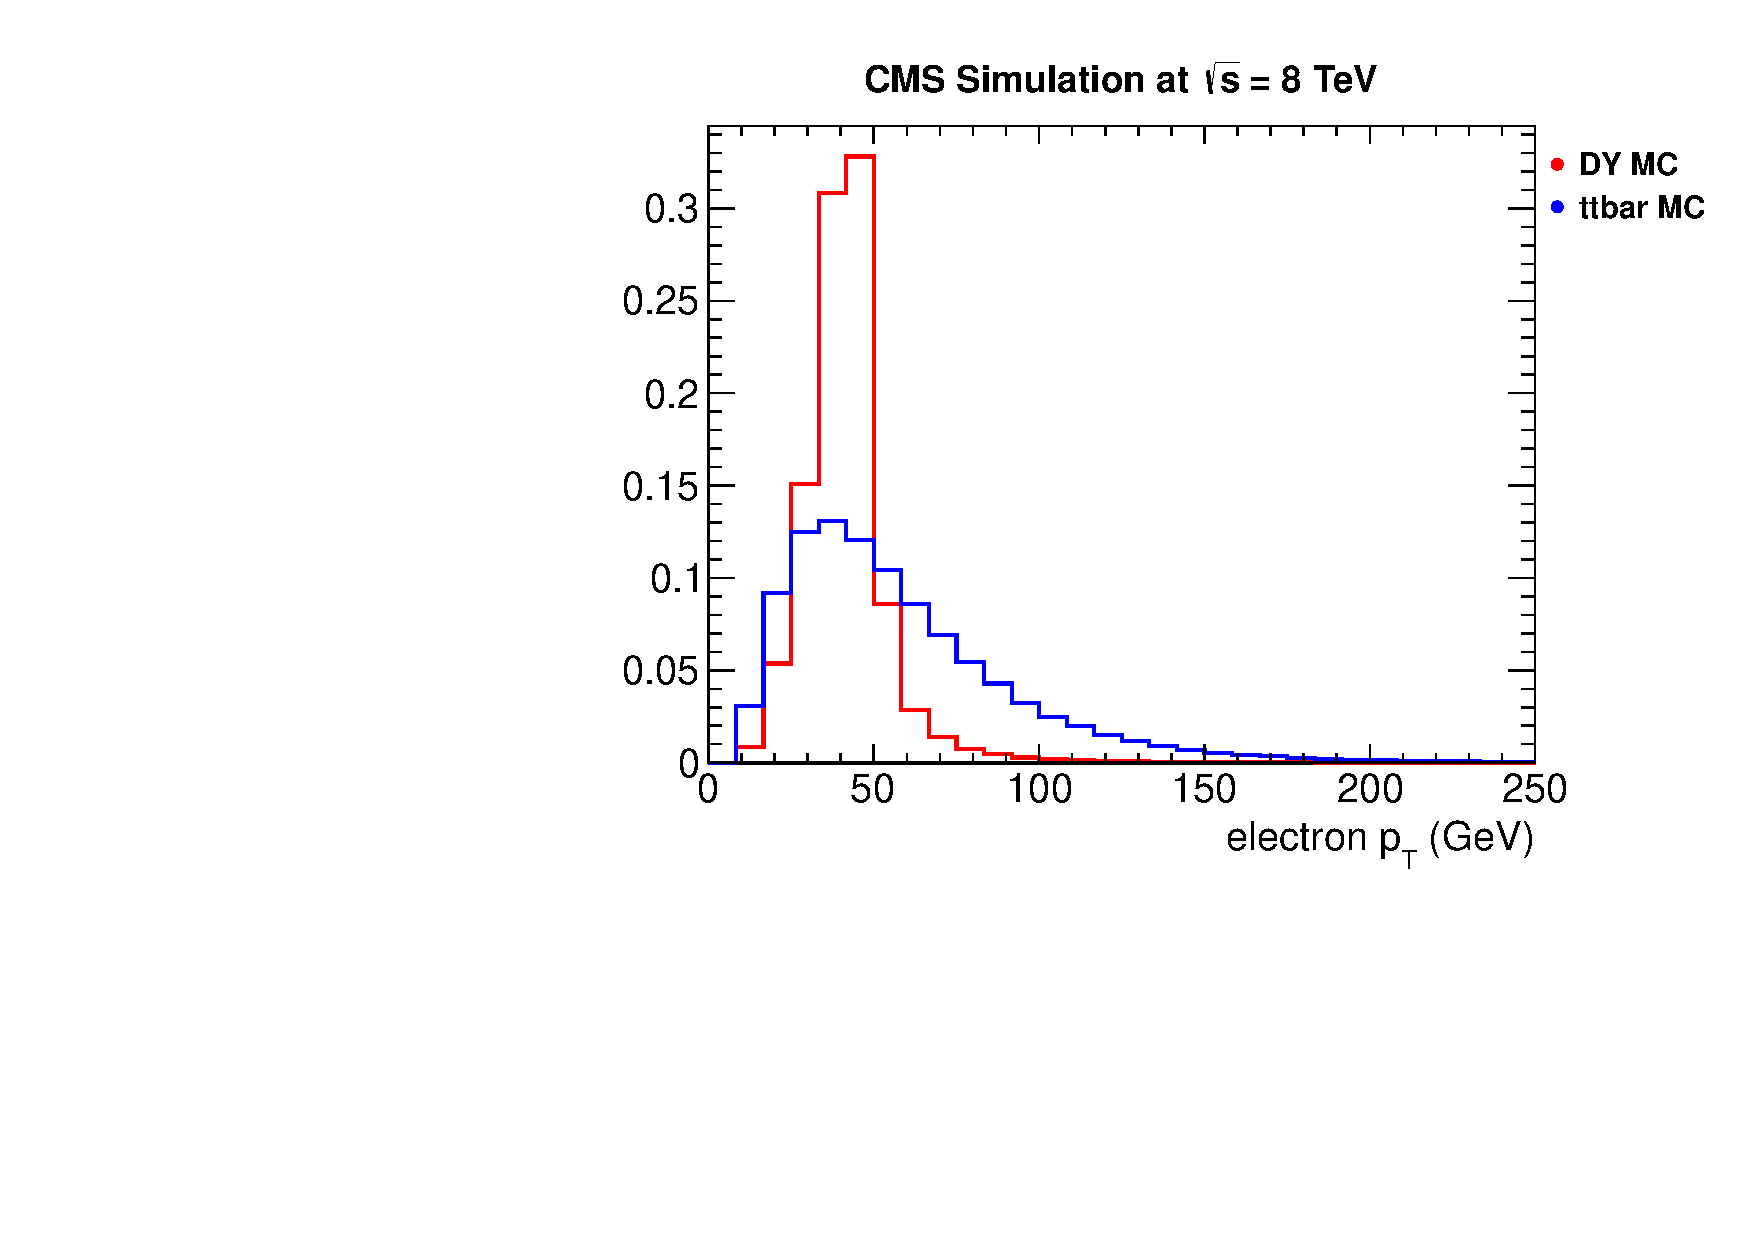
\includegraphics[width=0.8\textwidth]{p_flips_vs_pt}
\caption[The \pt distribution for electrons that pass the analysis selections]
{\label{fig:bkgd_flips_vs_pt}
The \pt distribution for electrons that pass the selections from
Section~\ref{sec:evtsel_el} for Drell-Yan and \ttbar simulated events.
}
\end{center}
\end{figure}

% --------------------------------------------------------------------------- %
We calculate the flip rate as a fraction. The denominator is the
number of electrons that pass the full selection requirements (see
Section~\ref{sec:evtsel_el}). The numerator is the number of denominator
electrons with an incorrectly reconstructed charge sign according to truth
information from the simulation. We further calculate this in bins of \pt and
\aeta. The result is shown in table \ref{tab:bkgd_flips_rate}. Notice that the
flip rate has a very significant dependence on both \pt and \aeta.
% --------------------------------------------------------------------------- %
\begin{table}[hbt!]
\begin{center}
\caption[Electron charge-flip rate as a function of \pt and \aeta]
{\label{tab:bkgd_flips_rate}
Electron charge-flip rate as a function of \pt and \aeta.
}
\end{center}
\resizebox{0.55\textwidth}{!}{\begin{minipage}{\textwidth}
\begin{tabular}{c|ccccc}
\hline\hline
\backslashbox{$|\eta|$}{$p_T$} & 0-20 \GeV                         & 20-40 \GeV                        & 40-60 \GeV                        & 60-80 \GeV                        & 80-200 \GeV                       \\ \hline
0.0-1.0                        & $2.52\ten{-05} \pm 2.52\ten{-05}$ & $3.44\ten{-05} \pm 6.18\ten{-06}$ & $2.06\ten{-05} \pm 4.38\ten{-06}$ & $1.03\ten{-04} \pm 3.27\ten{-05}$ & $9.16\ten{-05} \pm 4.58\ten{-05}$ \\
1.0-2.0                        & $1.67\ten{-04} \pm 6.29\ten{-05}$ & $1.81\ten{-04} \pm 1.82\ten{-05}$ & $2.16\ten{-04} \pm 1.94\ten{-05}$ & $5.31\ten{-04} \pm 1.00\ten{-04}$ & $9.87\ten{-04} \pm 2.06\ten{-04}$ \\
2.0-2.4                        & $0.00\ten{+00} \pm 4.52\ten{-05}$ & $2.96\ten{-04} \pm 4.52\ten{-05}$ & $3.96\ten{-04} \pm 5.49\ten{-05}$ & $1.34\ten{-03} \pm 3.34\ten{-04}$ & $8.79\ten{-04} \pm 4.39\ten{-04}$ \\
\hline\hline
\end{tabular}
\end{minipage}
}
\end{table}

% --------------------------------------------------------------------------- %
We validate by making a prediction and an observation using the flip rate
applied to data. We start by selecting electron pairs that pass the analysis
\pt, \aeta, and electron ID and isolation requirements which are listed
in Section \ref{sec:evtsel_el}. Also, these events must pass the dilepton
trigger (for data) from Section~\ref{sec:evtsel_trig}, and the dilepton
invariant mass should be between 76 \GeV and 106 \GeV for exactly one pair of
electrons. The observation is then simply the number of same sign dilepton
events occurring in the above dilepton selection. For the prediction, the flip
rate (which was derived in simulation) is applied to this selection: we select the
opposite-sign dielectron events in the sample, weighting each one with a factor
of
% --------------------------------------------------------------------------- %
\[ 
\frac{\epsilon_{fl,1}}{1 - \epsilon_{fl,1}} + \frac{\epsilon_{fl,2}}{1 - \epsilon_{fl,2}}
\]
% --------------------------------------------------------------------------- %
where the flip rate for the nth electron, $\epsilon_{fl, n}$, is taken from
table \ref{tab:bkgd_flips_rate}. The denominator is necessary because we are
not summing over the same-sign dielectron pairs.
 
In data, we predict 944 same-sign events and observe 1561 events. The
invariant mass distribution for these 1561 events is shown in figure
\ref{fig:bkgd_flips_ss_mee}. However, we must investigate the possibility of
non-Z events occurring in the data sample, causing our observation to be
artificially high.
% --------------------------------------------------------------------------- %
\begin{figure}[!hbt]
\begin{center}
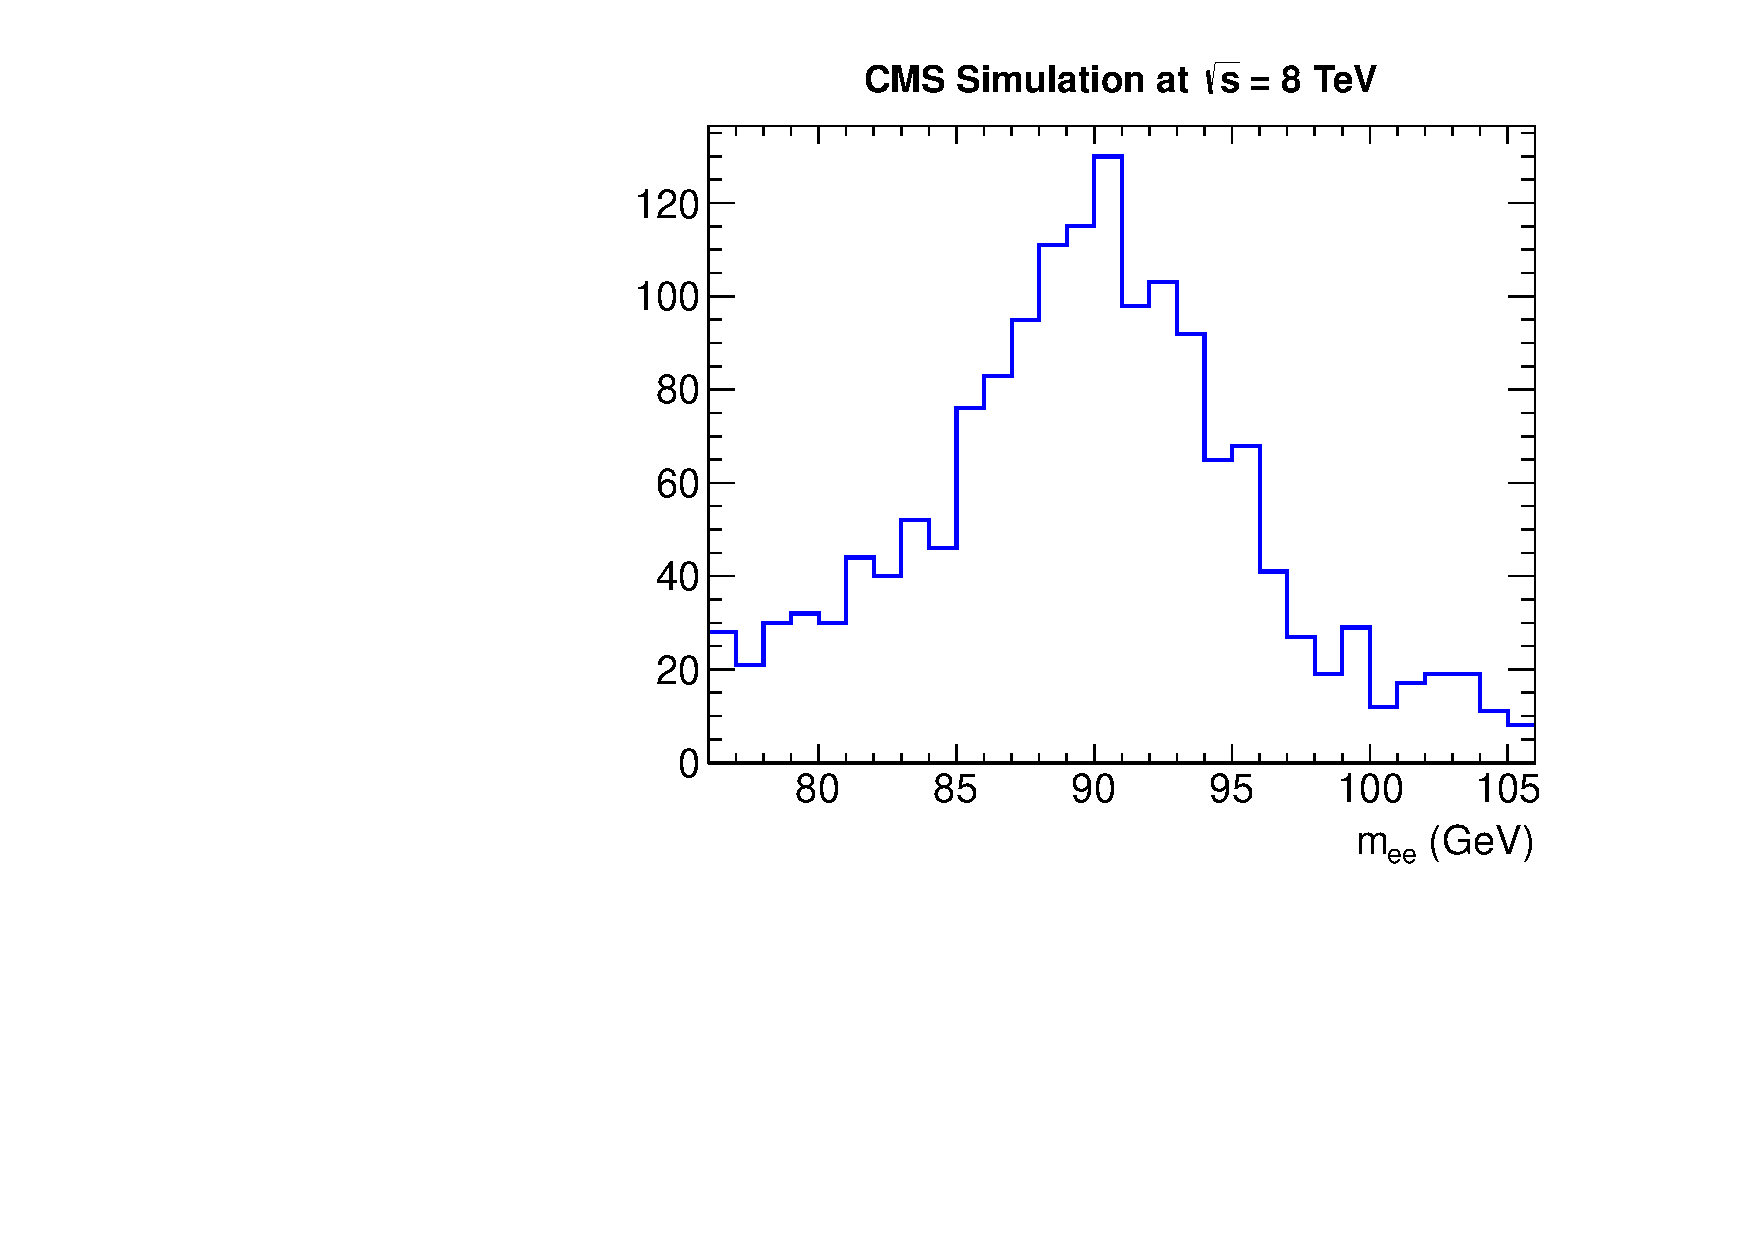
\includegraphics[width=0.8\textwidth]{p_ss_mee}
\caption[The \mee distribution for same-sign electron pairs in data]
{\label{fig:bkgd_flips_ss_mee}
The \mee distribution for same-sign electron pairs in data.
}
\end{center}
\end{figure}

% --------------------------------------------------------------------------- %
We consider the upper sidebands in the dilepton mass plot of the data charge
flips ($106\ \GeV < \mee < 121\ \GeV$). Figure \ref{fig:bkgd_flips_mee} shows
that events in this region are unlikely to be flips from high mass Zs, and
so we may assume as an approximation that everything in this region is a
contamination. Figure \ref{fig:bkgd_flips_ss_mee} shows that a significant
number of electrons are indeed predicted in this region. In order to compare
with the prediction from simulation, we subtract these events from the full
data prediction. We extrapolate from this figure that about 16\% of the
observed flips are actually contamination rather than charge flips. We use this
factor to adjust our number of observed charge flips.
% --------------------------------------------------------------------------- %
\begin{figure}[!hbt]
\begin{center}
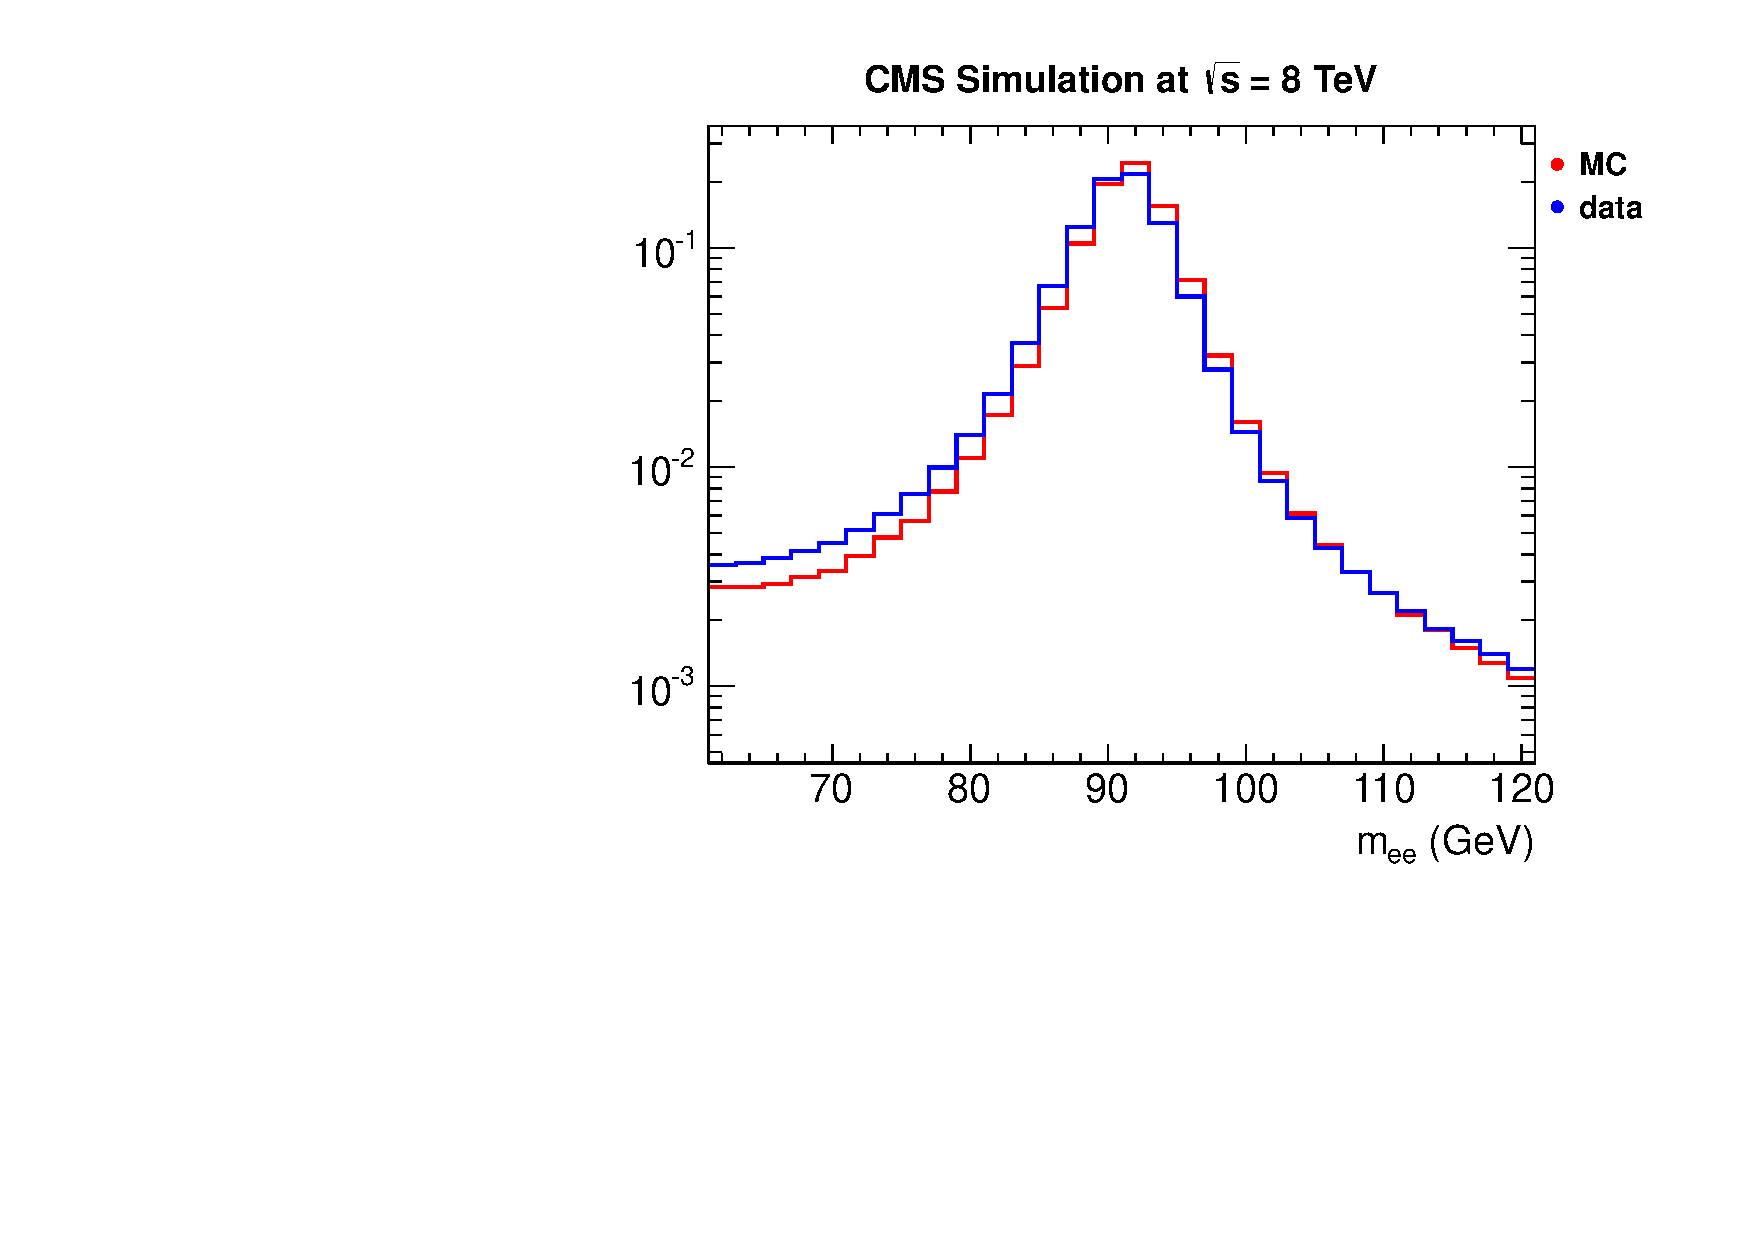
\includegraphics[width=0.8\textwidth]{p_os_mee}
\caption[The \mee distribution for opposite-sign electron pairs in data]
{\label{fig:bkgd_flips_mee}
The \mee distribution for opposite-sign electron pairs in data.
}
\end{center}
\end{figure}

% --------------------------------------------------------------------------- %
The result is that we expect 944 charge flips, and we observe 1311. We
reconcile these two differences with a scale factor:
\[ SF = \textrm{observed/predicted} = 1.39 \]
So the flip rates in Table~\ref{tab:bkgd_flips_rate}, multiplied by the scale
factor, should give a good approximation of the overall flip rate.

This remaining discrepancy, coupled with the kinematic limitation of the       
control sample, allow for considerable error in our estimation of the charge   
flip background. We therefore assign an overall systematic of $\pm\ 30\%$ to   
allow for these.                                                               

% --------------------------------------------------------------------------- %
% --------------------------------------------------------------------------- %
\section{Rare SM background estimation}
\label {sec:bkgd_rare}
% --------------------------------------------------------------------------- %
% --------------------------------------------------------------------------- %
Backgrounds arising from failures of lepton identification and electron charge
mis-reconstruction together account for 40-70\% of the estimated background in
a given search region. The remaining 30-60\% of the background is irreducible
and is taken directly from simulation. A list of the process and associated
cross sections is provided in Table~\ref{tab:evtsel_datasets_rare} and repeated
here for convenience. Note that we neglect contributions from $W\gamma^{*}
\rightarrow \ell \nu ee$ because the simulated dataset was known to be faulty
and this process contributes less than a percent to the irreducible background
total.
% --------------------------------------------------------------------------- %
%\begin{landscape}
\begin{table}[!hbt]
\begin{center}
\caption[Sources of true same-sign dileptons from Standard Model processes]
{\label{tab:bkgd_datasets_mc}
Sources of true same-sign dileptons from Standard Model processes. Cross
sections are next-to-leading order. The equivalent integrated luminosity
of these simulated events is listed in the column on the far right. The
contributions from these process to the background is taken directly from
simulation.
}
\footnotesize{
    \begin{tabular}{lccc}
    \hline\hline
    Sample     & Cross Section (pb) & Equivalent Luminosity (\fbinv) \\ \hline
    \ttZ       & 0.208              & 1021                           \\
    \ttW       & 0.232              & 845                            \\
    \ttWW      & 0.00204            & 106931                         \\
    \ttG       & 2.17               & 33                             \\
    \tbZ       & 0.0114             & 13026                          \\
    \ZZZ       & 0.00554            & 40692                          \\
    \WWW       & 0.0822             & 2737                           \\
    \WWG       & 0.528              & 407                            \\
    \WZZ       & 0.0192             & 12946                          \\
    \WWZ       & 0.0580             & 3832                           \\
    \ZZ        & 0.177              & 27177                          \\
    \WZ        & 1.058              & 1908                           \\
    \qqWmWm    & 0.0889             & 1084                           \\
    \qqWpWp    & 0.248              & 402                            \\
    \WWdps     & 0.588              & 1418                           \\
    \Wgsmm     & 1.91               & 156                            \\
    \Wgstt     & 0.336              & 148                            \\
    \HToWW     & 0.260              & 769                            \\
    \HToZZ     & 0.0320             & 15652                          \\
    \HToTauTau & 0.0177             & 5478                           \\
    \hline\hline
    \end{tabular}
}
\end{center}
\end{table}

% --------------------------------------------------------------------------- %
Most of the background involving rare SM process have never been measured
before. The cross sections used for these processes are next-to-leading (NLO)
order and are used to normalize the rare predictions. The cross section values
used for the most relevant processes, \ttW and \ttZ, are 232 \fb and 208 \fb,
respectively~\cite{ttw,ttz}. The systematic uncertainty for the rare SM
backgrounds accounts for the theoretical uncertainty on the cross sections as
well as for the ratio between LO (as in simulation) and NLO cross-sections being
non-uniform as a function of jet multiplicity, \Ht and \met. Due to this, a
50\% systematic uncertainty for the prediction from these rare SM processes is
assigned.

% --------------------------------------------------------------------------- %
% --------------------------------------------------------------------------- %
\chapter{Selection Efficiencies}
\label {ch:eff}
% --------------------------------------------------------------------------- %
% --------------------------------------------------------------------------- %
Selection efficiencies is one of the ingredients needed to measure a cross
section or set an exclusion limit. The combined selection efficiency represents
the fraction of events within the acceptance that are also reconstructed and
pass the analysis selections. Acceptances here is defined as the probability
for a generated object from simulation to actually traverse through the
detector. It is customary to measure the efficiency for the various aspects of
the selections and then combine them as a measure of the total efficiency of
the analysis.

To determine where a specific model is consistent with the data, the same
analysis selections are applied to a simulated sample of this model. Here, the
simulation has been generated with a Monte Carlo generator that has been
passed through the detector simulation and then the full off-line reconstruction.
No trigger requirement is made in the simulation. Instead, we scale the
simulated events by the trigger efficiency measured for the relevant signature.
Similarly, differences exist in the efficiency of the lepton identification
and isolation requirements, as well as the b-tagging efficiency between data
and simulation. Scale factors are measured and then applied to simulation to
account for these differences.

In this chapter we describe the techniques used to measure the selection
efficiencies and acceptances. The first section describes the measurement of
the lepton efficiencies using the \tnp method and its associated uncertainties.
The next section discusses the efficiencies for the various trigger
requirements. Finally, the \dmc scale factor for b-tagged jets is shown and the
procedure used to apply it is discussed.

% --------------------------------------------------------------------------- %
% --------------------------------------------------------------------------- %
\section{Lepton Efficiencies}
\label {sec:eff_lep}
% --------------------------------------------------------------------------- %
% --------------------------------------------------------------------------- %
The efficiencies of the lepton isolation and identification requirements
(including all quality requirements) are measured with the \tnp~method
in dilepton Z events using the full 2012 dataset. The efficiency of the
identification requirements is a property of the lepton itself and is directly
applicable to the leptons in signal events. The efficiency of the isolation
requirement, however, is a strong function of all other (mainly hadronic)
activity in the event. 

In this section, the lepton efficiencies are measured and their \dmc scale
factors are computed. The systematic uncertainty for this method is assigned
for both the \tnp method itself and due to the fact that the efficiency is
measured in Z events; however, our signal events will have more hadronic
activity and are more like \ttbar events. To account for this, a short study
is also done to show the validity of measuring the efficiency in Z events and
applying them to signal-like events.

% --------------------------------------------------------------------------- %
\subsection{Tag-and-Probe Method}
\label {sec:eff_tnp}
% --------------------------------------------------------------------------- %
The basic \tnp method essentially takes advantage of the fact that we can
reconstructed \Zll events with high accuracy. We select \Zlplm events from a
lepton triggered sample by requiring opposite-sign, same-flavor leptons in
a window around the nominal Z mass, $|m_Z - \mll| < 15~\GeV$. Out of window
events are not used to extract efficiencies but are retained as sidebands to
monitor the contaminations from backgrounds. Contributions from \W and QCD
processes are found to be small. An event is ``tagged'' by requiring one lepton
to pass the full lepton selection described in Chapter~\ref{ch:evtsel} and to
be matched to an online trigger object by requiring $\DR < 0.1$ to that object.
Tagged events are classified by the other ``probe'' leptons as either
% --------------------------------------------------------------------------- %
\begin{itemize}
\item Pass: The probe passes the full selection.
\item Fail: The probe fails the full selection but passes a looser criteria
chosen to not bias the selection under study.
\end{itemize}
% --------------------------------------------------------------------------- %
The ratio of the count of the passing probe leptons to the total number of
tagged events (both passing and failing probes) is the measured efficiency. The
efficiency is extracted in bins of \pt and \aeta for both electrons and muons
separately.

% --------------------------------------------------------------------------- %
\subsubsection{Tag-and-Probe Results for Electrons}
\label {sec:eff_tnp_el}
% --------------------------------------------------------------------------- %
The electron selection efficiencies are measured in events passing the
trigger, which require one well-identified electron passing the WP80
electron ID and with $\pt>27\ \GeV$ (see Table \ref{tab:evtsel_elid}). The
tag electron is required to match the well-identified electron from the
\verb=HLT_Ele27_WP80= trigger and also to pass all the electron requirements
described in Section~\ref{sec:evtsel_el}. Additionally, the tag electron is
chosen to have a $\pt>32\ \GeV$ to eliminate turn-on effects from the trigger
efficiency. The probe electron is required to pass a simple loose selection as
follows

\begin{itemize}
\item reconstructed electron
\item $\pt > 10\ \GeV$,
\item $\aeta < 2.4$, 
\item excluding electrons with a supercluster between $1.4442 < |\eta_{SC}| < 1.566$.
\end{itemize}

The isolation efficiency is measured with the probes passing all electron
selections described in Section~\ref{sec:evtsel_el}, except for the isolation
itself. The identification efficiency is measured with probes passing the
isolation requirement. The overall efficiency is measured with probes passing
only the nominal requirements above. Results of the measurement are summarized
in Table~\ref{tab:eff_tnp_el}. The contribution from the Z events in data is
based on fitting the mass range 60-120 \GeVcc~using a simultaneous fit of
various models for the signal and backgrounds. The models used are summarized
in the following Table~\ref{tab:eff_tnp_models}. Since the kinematics of the
background shape varies in the different $\pt-\aeta$ bins, different background
shapes were chosen on a bin-by-bin basis in order to get the best fits. The
results of the \tnp show a strong dependence on the lepton \pt and a weaker but
non-negligible dependence on \aeta.
% --------------------------------------------------------------------------- %
\begin{table}[!htb]
\caption[Models used for measuring the signal or the background contribution in the \tnp~method]
{\label{tab:eff_tnp_models}
Models used for measuring the signal or the background contribution in the \tnp~method.
}
\begin{center}
\begin{tabular}{l|l}
\hline\hline
Model                                              & Usage      \\ \hline
Breit-Wigner function $\ast$ Crystal-Ball function & Signal     \\
MC-based template function                         & Signal     \\ \hline
Exponential                                        & Background \\
Exponential $\ast$ error function                  & Background \\
Polynomial                                         & Background \\
Polynomial $\times$ exponential function           & Background \\
Chebyshev Polynomial                               & Background \\
\hline\hline
\end{tabular}
\end{center}
\end{table}
% --------------------------------------------------------------------------- %
\begin{table}[!hbt]
\begin{center}
\caption[Electron efficiencies measured using the \tnp~method]
{\label{tab:eff_tnp_el}
Electron efficiencies measured using the \tnp~method.  The uncertainties are statistical only.
}
\end{center}
\resizebox{0.65\textwidth}{!}{\begin{minipage}{\textwidth}
\begin{tabular}{c|c|c|c|c|c|c|c}
\hline\hline
\backslashbox{\aeta}{\pt}     &         & $10-15$ \GeV      & $15-20$ \GeV      & $20-30$ \GeV      & $30-40$ \GeV      & $40-50$ \GeV      & $50-200$ \GeV     \\ \hline \hline
\multirow{3}{*}{$0.0-0.8$}    & MC      & 0.363 $\pm$ 0.004 & 0.503 $\pm$ 0.002 & 0.646 $\pm$ 0.001 & 0.764 $\pm$ 0.000 & 0.819 $\pm$ 0.000 & 0.841 $\pm$ 0.001 \\
                              & Data    & 0.303 $\pm$ 0.003 & 0.462 $\pm$ 0.002 & 0.617 $\pm$ 0.001 & 0.733 $\pm$ 0.000 & 0.796 $\pm$ 0.000 & 0.815 $\pm$ 0.001 \\
                              & Data/MC & 0.834 $\pm$ 0.012 & 0.918 $\pm$ 0.006 & 0.954 $\pm$ 0.002 & 0.960 $\pm$ 0.001 & 0.972 $\pm$ 0.001 & 0.969 $\pm$ 0.001 \\ \hline
\multirow{3}{*}{$0.8-1.4442$} & MC      & 0.379 $\pm$ 0.004 & 0.480 $\pm$ 0.003 & 0.600 $\pm$ 0.001 & 0.736 $\pm$ 0.001 & 0.809 $\pm$ 0.000 & 0.830 $\pm$ 0.001 \\
                              & Data    & 0.369 $\pm$ 0.008 & 0.435 $\pm$ 0.003 & 0.554 $\pm$ 0.001 & 0.688 $\pm$ 0.001 & 0.772 $\pm$ 0.000 & 0.794 $\pm$ 0.001 \\
                              & Data/MC & 0.973 $\pm$ 0.023 & 0.906 $\pm$ 0.009 & 0.923 $\pm$ 0.003 & 0.935 $\pm$ 0.001 & 0.955 $\pm$ 0.001 & 0.956 $\pm$ 0.001 \\ \hline
\multirow{3}{*}{$1.566-2.0$}  & MC      & 0.206 $\pm$ 0.004 & 0.344 $\pm$ 0.003 & 0.482 $\pm$ 0.002 & 0.615 $\pm$ 0.001 & 0.681 $\pm$ 0.001 & 0.697 $\pm$ 0.001 \\
                              & Data    & 0.197 $\pm$ 0.004 & 0.313 $\pm$ 0.003 & 0.444 $\pm$ 0.002 & 0.569 $\pm$ 0.001 & 0.647 $\pm$ 0.001 & 0.693 $\pm$ 0.001 \\
                              & Data/MC & 0.954 $\pm$ 0.028 & 0.909 $\pm$ 0.012 & 0.921 $\pm$ 0.005 & 0.924 $\pm$ 0.002 & 0.950 $\pm$ 0.001 & 0.995 $\pm$ 0.002 \\ \hline
\multirow{3}{*}{$2.0-2.4$}    & MC      & 0.199 $\pm$ 0.004 & 0.321 $\pm$ 0.004 & 0.419 $\pm$ 0.002 & 0.515 $\pm$ 0.001 & 0.576 $\pm$ 0.001 & 0.593 $\pm$ 0.002 \\
                              & Data    & 0.223 $\pm$ 0.005 & 0.303 $\pm$ 0.004 & 0.416 $\pm$ 0.000 & 0.494 $\pm$ 0.001 & 0.558 $\pm$ 0.001 & 0.575 $\pm$ 0.002 \\
                              & Data/MC & 1.119 $\pm$ 0.036 & 0.944 $\pm$ 0.015 & 0.993 $\pm$ 0.004 & 0.959 $\pm$ 0.003 & 0.968 $\pm$ 0.002 & 0.969 $\pm$ 0.004 \\ \hline \hline
\end{tabular}
\end{minipage}
}
\end{table}
% --------------------------------------------------------------------------- %

The following sources of systematic uncertainty are attributed to this
measurement: variation in the models used to fit the signal and background
distributions and measuring the isolation (Iso) and identification (ID)
components simultaneously (ID+Iso) as opposed to a factorized measurement
(ID*Iso). Varying the models for signal and backgrounds seems to make the
most significant difference to the data-to-MC scale factors in the lowest \pt
bins where the backgrounds are the largest and least understood. The effect
was sub-dominant to the difference in factorization scheme (using ID+Iso vs
ID*Iso). To show the difference between the data-to-MC scale factors using
different factorization schemes, the relative difference of the data-to-MC
scale factors when measured using ID+Iso versus ID*Iso is shown in the
following Table~\ref{tab:eff_tnp_el_fac}. As you move to lower \pt~and higher
\aeta, we see relatively larger differences between the two factorization
schemes with some differences as high as~$\sim 25\%$. The two methods offer a
trade off with the ID+Iso method accounting for the correlation between the
ID and isolation; whereas, the ID*Iso does not account for the correlation
but has a smaller background. This leads to differences in the efficiencies
between the two methods. At higher \pt~and lower \aeta, we see this effect is
mitigated with relative differences on the order of a few percent. To account
for these differences, we apply at 10\% systematic uncertainty for electrons
with $\pt<15\ \GeV$ where we saw larger differences and 5\% above where the
differences settle out.
% --------------------------------------------------------------------------- %
\begin{table}[!hbt]
\begin{center}
\caption[Electron efficiency data-to-mc scale factors measured using the \tnp~method]
{\label{tab:eff_tnp_el_fac}
Electron efficiency data-to-MC scale factors measured using the \tnp~method in
different factorization schemes. ``rel diff'' refers to the relative difference
between the two factorization schemes. The uncertainties are statistical only.
}
\end{center}
\resizebox{0.65\textwidth}{!}{\begin{minipage}{\textwidth}
\begin{tabular}{c|c|c|c|c|c|c|c}
\hline\hline
\backslashbox{\aeta}{\pt}     &          & $10-15$ \GeV      & $15-20$ \GeV       & $20-30$ \GeV       & $30-40$ \GeV       & $40-50$ \GeV       & $50-200$ \GeV      \\ \hline \hline
\multirow{3}{*}{$0.0-0.8$}    & ID*Iso   & 0.787 $\pm$ 0.022 & 0.943 $\pm$ 0.010  & 0.963 $\pm$ 0.002  & 0.969 $\pm$ 0.001  & 0.975 $\pm$ 0.000  & 0.973 $\pm$ 0.001  \\
                              & ID+Iso   & 0.834 $\pm$ 0.012 & 0.918 $\pm$ 0.006  & 0.954 $\pm$ 0.002  & 0.960 $\pm$ 0.001  & 0.972 $\pm$ 0.001  & 0.969 $\pm$ 0.001  \\
                              & rel diff & 0.055 $\pm$ 0.030 & -0.028 $\pm$ 0.013 & -0.009 $\pm$ 0.003 & -0.010 $\pm$ 0.001 & -0.004 $\pm$ 0.001 & -0.004 $\pm$ 0.002 \\ \hline
\multirow{3}{*}{$0.8-1.4442$} & ID*Iso   & 0.861 $\pm$ 0.015 & 0.910 $\pm$ 0.011  & 0.921 $\pm$ 0.002  & 0.943 $\pm$ 0.001  & 0.956 $\pm$ 0.001  & 0.950 $\pm$ 0.002  \\
                              & ID+Iso   & 0.973 $\pm$ 0.023 & 0.906 $\pm$ 0.009  & 0.923 $\pm$ 0.003  & 0.935 $\pm$ 0.001  & 0.955 $\pm$ 0.001  & 0.956 $\pm$ 0.001  \\
                              & rel diff & 0.115 $\pm$ 0.029 & -0.005 $\pm$ 0.015 & 0.003 $\pm$ 0.004  & -0.009 $\pm$ 0.001 & -0.001 $\pm$ 0.001 & 0.006 $\pm$ 0.003  \\ \hline
\multirow{3}{*}{$1.566-2.0$}  & ID*Iso   & 0.798 $\pm$ 0.028 & 0.886 $\pm$ 0.026  & 0.910 $\pm$ 0.005  & 0.928 $\pm$ 0.002  & 0.948 $\pm$ 0.001  & 0.964 $\pm$ 0.002  \\
                              & ID+Iso   & 0.954 $\pm$ 0.028 & 0.909 $\pm$ 0.012  & 0.921 $\pm$ 0.005  & 0.924 $\pm$ 0.002  & 0.950 $\pm$ 0.001  & 0.995 $\pm$ 0.002  \\
                              & rel diff & 0.164 $\pm$ 0.042 & 0.025 $\pm$ 0.031  & 0.012 $\pm$ 0.008  & -0.004 $\pm$ 0.003 & 0.002 $\pm$ 0.002  & 0.031 $\pm$ 0.003  \\ \hline
\multirow{3}{*}{$2.0-2.4$}    & ID*Iso   & 0.866 $\pm$ 0.027 & 0.929 $\pm$ 0.015  & 0.935 $\pm$ 0.005  & 0.954 $\pm$ 0.002  & 0.962 $\pm$ 0.002  & 0.955 $\pm$ 0.004  \\
                              & ID+Iso   & 1.119 $\pm$ 0.036 & 0.944 $\pm$ 0.015  & 0.993 $\pm$ 0.004  & 0.959 $\pm$ 0.003  & 0.968 $\pm$ 0.002  & 0.969 $\pm$ 0.004  \\
                              & rel diff & 0.226 $\pm$ 0.041 & 0.016 $\pm$ 0.023  & 0.058 $\pm$ 0.007  & 0.006 $\pm$ 0.004  & 0.006 $\pm$ 0.003  & 0.015 $\pm$ 0.006  \\ \hline \hline
\end{tabular}
\end{minipage}
}
\end{table}

% --------------------------------------------------------------------------- %
\subsubsection{Tag-and-Probe Results for Muons}
\label {sec:eff_tnp_mu}
% --------------------------------------------------------------------------- %
For muons, the technique for electrons is essentially repeated with appropriate
modifications for muon specific selections. The muon selection efficiencies are
measured using events that pass the \verb=HLT_IsoMu24_eta2p1= trigger which
require one isolated muon with a $\pt>24\ \GeV$. In the \tnp~analysis, the
tag muon is required to match the well-identified muon from the trigger and
also to pass all the muon requirements described in Section~\ref{sec:evtsel_mu}.
Additionally, the tag muon is chosen to have a $\pt>30\ \GeV$ to eliminate
turn-on effects from the trigger efficiency. The probe muon is required to have
% --------------------------------------------------------------------------- %
\begin{itemize}
  \item $\pt > 10\ \GeV$
  \item $\aeta < 2.4$
  \item have both the global and the particle-flow muon types.
\end{itemize}
% --------------------------------------------------------------------------- %
The isolation efficiency is measured with the probes passing all muon
selections described in Section~\ref{sec:evtsel_mu}, except for the isolation
itself. The identification efficiency is measured with probes passing the
isolation requirement. The overall efficiency is measured with probes passing
only the nominal requirements above. Results of the measurement are summarized
in Table~\ref{tab:eff_tnp_mu}. The contribution from the Z events in data
is based on fitting the mass range of 60-120 \GeVcc~using a simultaneous
fit of various models for the signal and backgrounds. The models used are
the same as those used by the electrons and are summarized in the same
Table~\ref{tab:eff_tnp_models}. Since the kinematics of the background shape
varied in the different $\pt-\aeta$ bins, different models were chosen on a
bin-by-bin basis in order to get the best fits.
% --------------------------------------------------------------------------- %
\begin{table}[hb]
\begin{center}
\caption[Muon efficiencies measured using the \tnp~method]
{\label{tab:eff_tnp_mu}
Muon efficiencies measured using the \tnp~method. The uncertainties are
statistical only.
}
\end{center}
\resizebox{0.65\textwidth}{!}{\begin{minipage}{\textwidth}
\begin{tabular}{c|c|c|c|c|c|c|c}
\hline\hline
\backslashbox{\aeta}{\pt}  &         & $10-15$ \GeV      & $15-20$ \GeV      & $20-30$ \GeV      & $30-40$ \GeV      & $40-50$ \GeV      & $50-200$ \GeV     \\ \hline\hline
\multirow{3}{*}{$0.0-1.2$} & MC      & 0.582 $\pm$ 0.003 & 0.644 $\pm$ 0.002 & 0.754 $\pm$ 0.001 & 0.857 $\pm$ 0.000 & 0.901 $\pm$ 0.000 & 0.900 $\pm$ 0.000 \\
                           & Data    & 0.556 $\pm$ 0.005 & 0.617 $\pm$ 0.002 & 0.727 $\pm$ 0.001 & 0.832 $\pm$ 0.000 & 0.881 $\pm$ 0.000 & 0.877 $\pm$ 0.001 \\
                           & Data/MC & 0.956 $\pm$ 0.010 & 0.957 $\pm$ 0.004 & 0.964 $\pm$ 0.001 & 0.971 $\pm$ 0.000 & 0.978 $\pm$ 0.000 & 0.974 $\pm$ 0.001 \\ \hline
\multirow{3}{*}{$1.2-2.4$} & MC      & 0.646 $\pm$ 0.003 & 0.682 $\pm$ 0.002 & 0.763 $\pm$ 0.001 & 0.861 $\pm$ 0.000 & 0.907 $\pm$ 0.000 & 0.895 $\pm$ 0.001 \\
                           & Data    & 0.620 $\pm$ 0.010 & 0.662 $\pm$ 0.003 & 0.731 $\pm$ 0.001 & 0.843 $\pm$ 0.000 & 0.892 $\pm$ 0.000 & 0.875 $\pm$ 0.001 \\
                           & Data/MC & 0.960 $\pm$ 0.016 & 0.971 $\pm$ 0.005 & 0.959 $\pm$ 0.001 & 0.978 $\pm$ 0.001 & 0.984 $\pm$ 0.000 & 0.977 $\pm$ 0.001 \\ \hline\hline
\end{tabular}
\end{minipage}
}
\end{table}

% --------------------------------------------------------------------------- %
Since the technique for the muons is the same as the electrons, we consider
the same sources of systematic uncertainties. As with the electrons, varying
the fitting models showed the most difference in the lower \pt~bins for the
same reason. Also, the factorization scheme was varied with the results shown
in Table~\ref{tab:eff_tnp_mu_fac}. As you move to lower \pt~and higher \aeta,
we see differences between the two factorization schemes of~$\sim
5\%$. At higher \pt~and lower \aeta, we see this effect is much smaller being
a few percent or less. To account for these differences, we apply at 5\%
systematic uncertainty for muons with $\pt<15\ \GeV$ where we saw larger
differences and 3\% above where the differences settle out.

\begin{table}[hb]
\begin{center}
\caption[Muon efficiency data-to-mc scale factors measured using the \tnp~method]
{\label{tab:eff_tnp_mu_fac}
Muon efficiency data-to-MC scale factors measured using the \tnp~method in
different factorization schemes. ``rel diff'' refers to the relative difference
between the two factorization schemes. The uncertainties are statistical only.
}
\end{center}
\resizebox{0.65\textwidth}{!}{\begin{minipage}{\textwidth}
\begin{tabular}{c|c|c|c|c|c|c|c}
\hline\hline
\backslashbox{\aeta}{\pt}  &          & $10-15$ \GeV       & $15-20$ \GeV       & $20-30$ \GeV       & $30-40$ \GeV       & $40-50$ \GeV       & $50-200$ \GeV      \\ \hline\hline
\multirow{3}{*}{$0.0-1.2$} & ID*Iso   & 0.918 $\pm$ 0.017  & 0.955 $\pm$ 0.008  & 0.965 $\pm$ 0.001  & 0.972 $\pm$ 0.000  & 0.979 $\pm$ 0.000  & 0.974 $\pm$ 0.001  \\
                           & ID+Iso   & 0.956 $\pm$ 0.010  & 0.957 $\pm$ 0.004  & 0.964 $\pm$ 0.001  & 0.971 $\pm$ 0.000  & 0.978 $\pm$ 0.000  & 0.974 $\pm$ 0.001  \\
                           & rel diff & 0.040 $\pm$ 0.021  & 0.003 $\pm$ 0.009  & -0.001 $\pm$ 0.002 & -0.001 $\pm$ 0.001 & -0.001 $\pm$ 0.000 & -0.000 $\pm$ 0.001 \\ \hline
\multirow{3}{*}{$1.2-2.5$} & ID*Iso   & 0.962 $\pm$ 0.011  & 1.034 $\pm$ 0.006  & 0.972 $\pm$ 0.001  & 0.980 $\pm$ 0.001  & 0.985 $\pm$ 0.000  & 0.980 $\pm$ 0.001  \\
                           & ID+Iso   & 0.960 $\pm$ 0.016  & 0.971 $\pm$ 0.005  & 0.959 $\pm$ 0.001  & 0.978 $\pm$ 0.001  & 0.984 $\pm$ 0.000  & 0.977 $\pm$ 0.001  \\
                           & rel diff & -0.003 $\pm$ 0.020 & -0.065 $\pm$ 0.008 & -0.013 $\pm$ 0.002 & -0.002 $\pm$ 0.001 & -0.001 $\pm$ 0.001 & -0.003 $\pm$ 0.001 \\ \hline\hline
\end{tabular}
\end{minipage}
}
\end{table}

% --------------------------------------------------------------------------- %
\subsection{Lepton Composition}
\label {sec:eff_comp}
% --------------------------------------------------------------------------- %
In the previous sub-sections, we saw there there is an uncertainty associated
with the \dmc scale factors on the lepton efficiency. Another source of
uncertainty in the efficiencies measured above stems from the fact that the
efficiency is extracted from Drell-Yan (DY) events; however, the individual
efficiencies for ID and isolation for non-DY events may differ. A Monte
Carlo study was done to measure the ID and isolation efficiencies in \Zll
with respect to $\ttbar \rightarrow \ell\nu q \ell\nu q$ events. The exact
datasets used are listed in Appendix~\ref{sec:mc_details_sm}. The denominator
selection for these efficiencies was any generator-level e/$\mu$/$\tau$ ($\tau
\rightarrow e/\mu$) which is truth matched to a W/Z boson decay at the parton
level (Pythia6 status 3) within the acceptance and $\pt > 10\ \GeV$. The
numerator selection requires that this generated level lepton is truth matched
to a reconstructed lepton of the appropriate flavor which passes the full
analysis selection outlined in Chapter~\ref{ch:evtsel}. The results from this
study are shown in Figures~\ref{fig:eff_comp_el}, \ref{fig:eff_comp_mu} and in
Tables~\ref{tab:eff_comp_el}, \ref{tab:eff_comp_mu} for electrons and muons,
respectively.
% --------------------------------------------------------------------------- %
\begin{table}[!hbt]
\begin{center}
\caption[The electron efficiency relative differences between DY and \ttbar]
{\label{tab:eff_comp_el}
The electron efficiency relative differences between DY and \ttbar~
($(\epsilon_{DY} - \epsilon_{\ttbar})/\epsilon_{DY}$). The uncertainties are
statistical only.
}
\begin{tabular}{c|c|c}
\hline\hline
\backslashbox{\pt}{\aeta} & 0.00 - 1.44       & 1.57 - 2.50        \\\hline
10 - 20 \GeV              & 0.080 $\pm$ 0.021 &  0.094 $\pm$ 0.051 \\
20 - 30 \GeV              & 0.056 $\pm$ 0.011 &  0.021 $\pm$ 0.033 \\
30 - 40 \GeV              & 0.068 $\pm$ 0.009 &  -0.013 $\pm$ 0.030\\
40 - 50 \GeV              & 0.025 $\pm$ 0.009 &  -0.003 $\pm$ 0.030\\
50 - 70 \GeV              & 0.034 $\pm$ 0.007 &  0.038 $\pm$ 0.025 \\
70 - 100 \GeV             & 0.012 $\pm$ 0.010 &  0.033 $\pm$ 0.032 \\
100- 200 \GeV             & 0.021 $\pm$ 0.014 &  -0.027 $\pm$ 0.049\\ 
\hline\hline
\end{tabular}
\end{center}
\end{table}
% --------------------------------------------------------------------------- %
\begin{figure}[!hbt]
\begin{center}
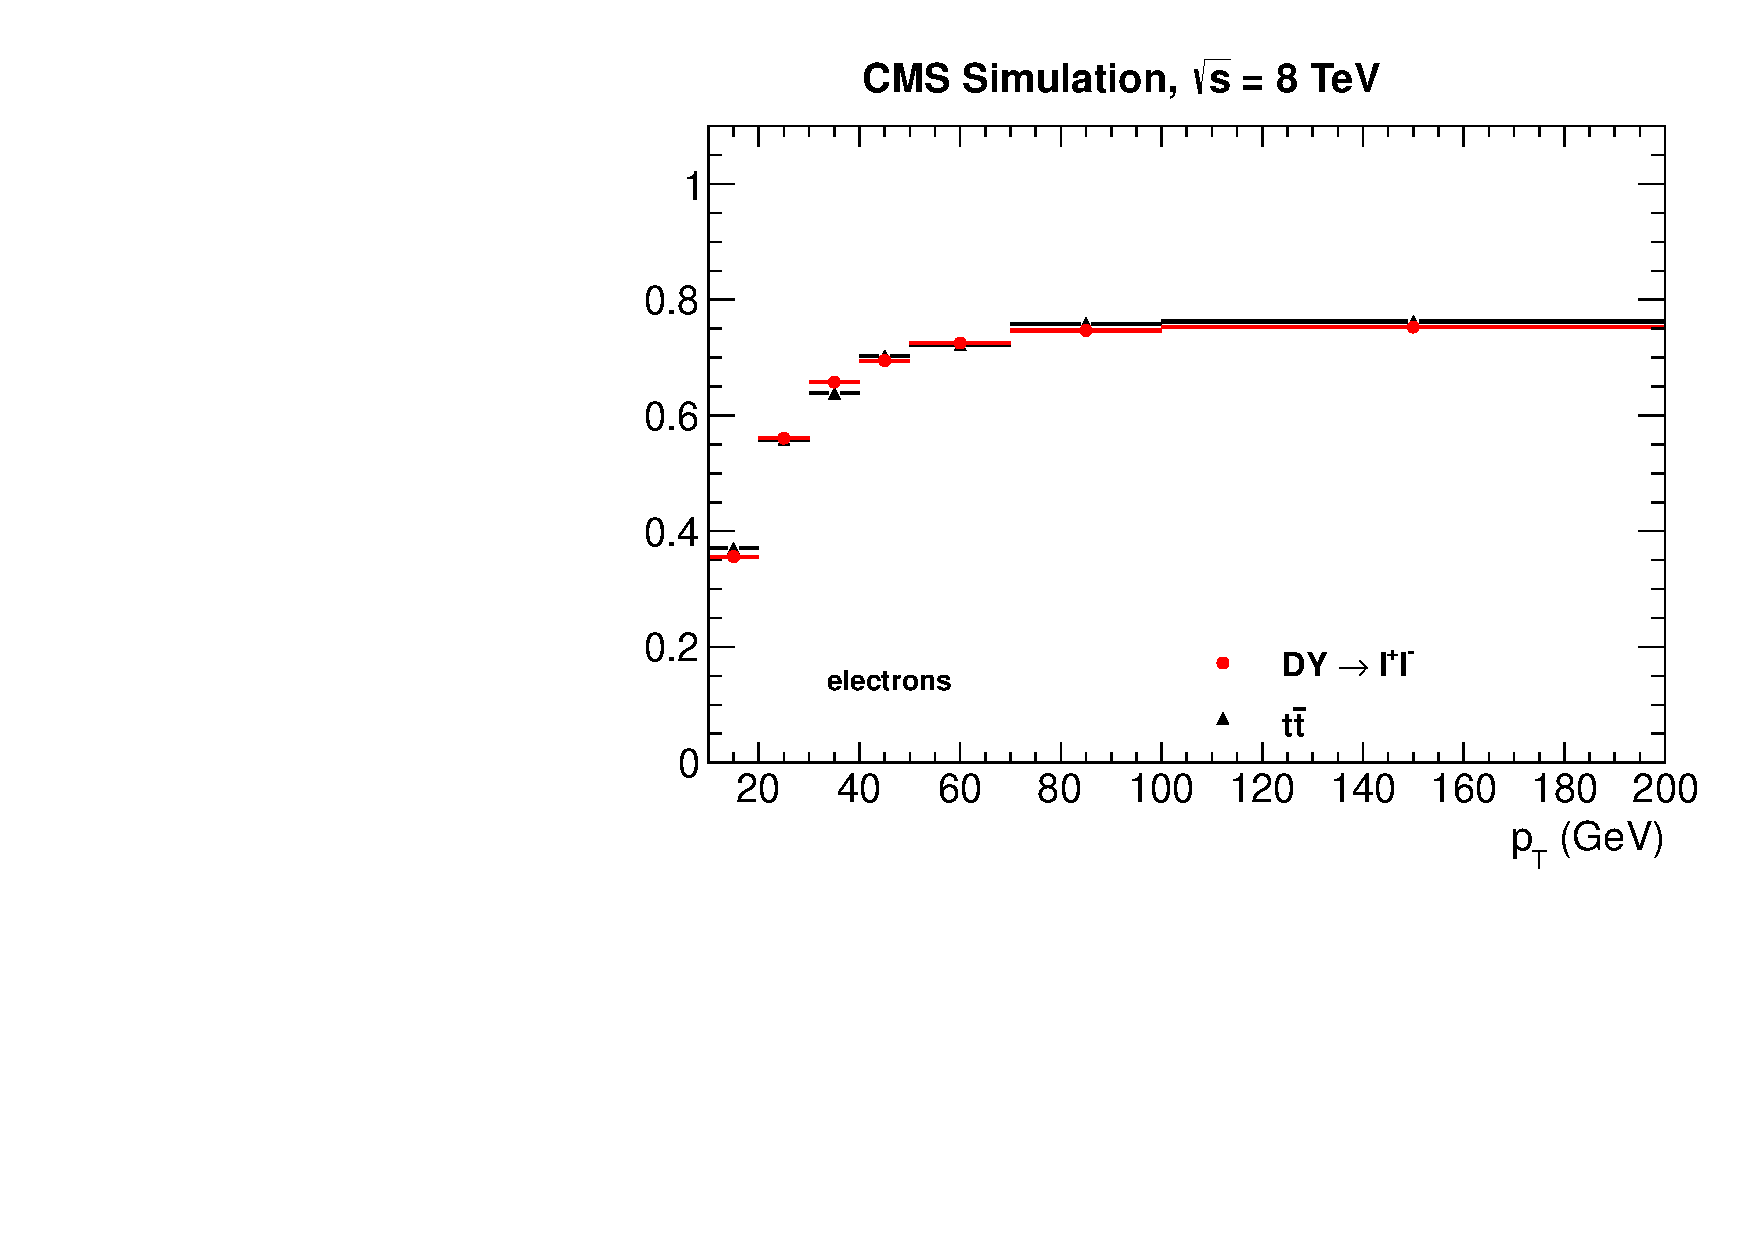
\includegraphics[width=0.49\linewidth]{p_eff_el_vs_pt}
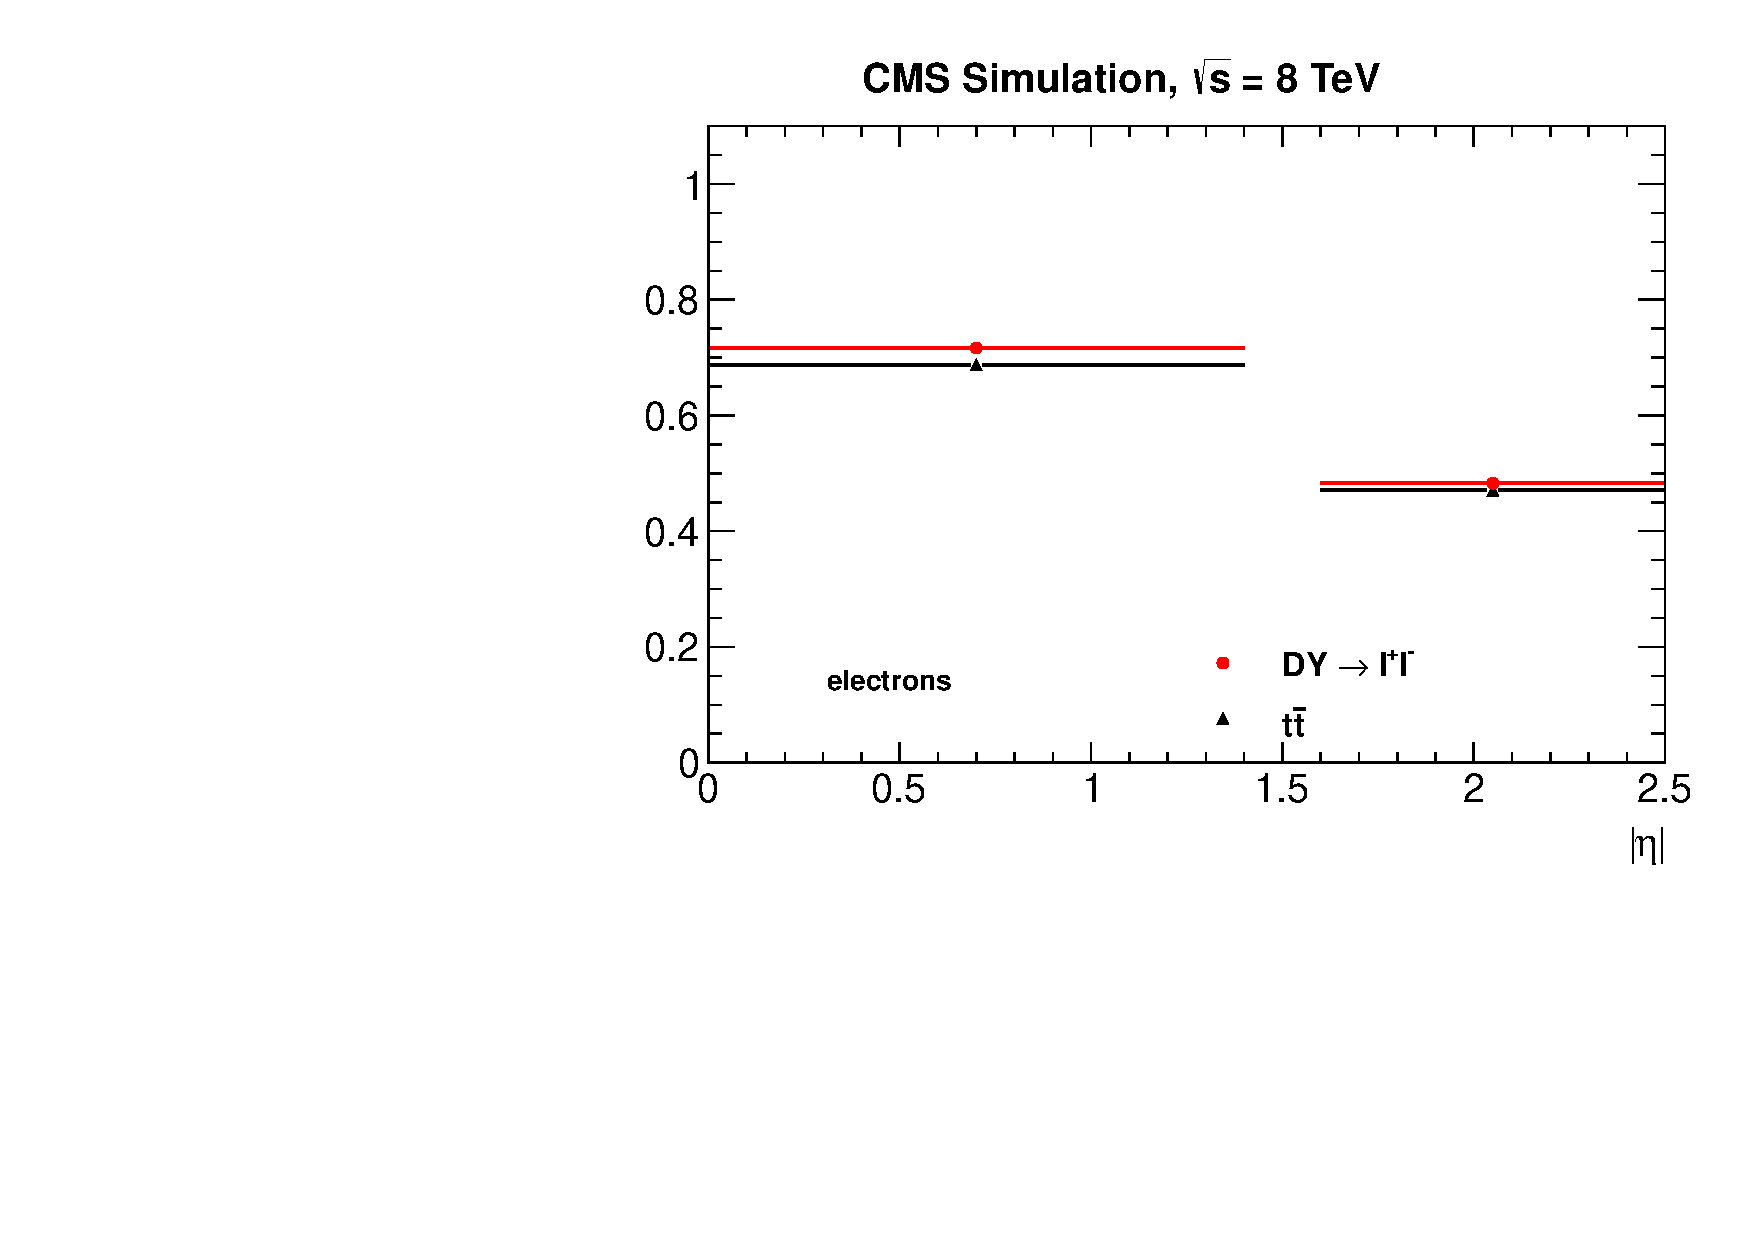
\includegraphics[width=0.49\linewidth]{p_eff_el_vs_eta}
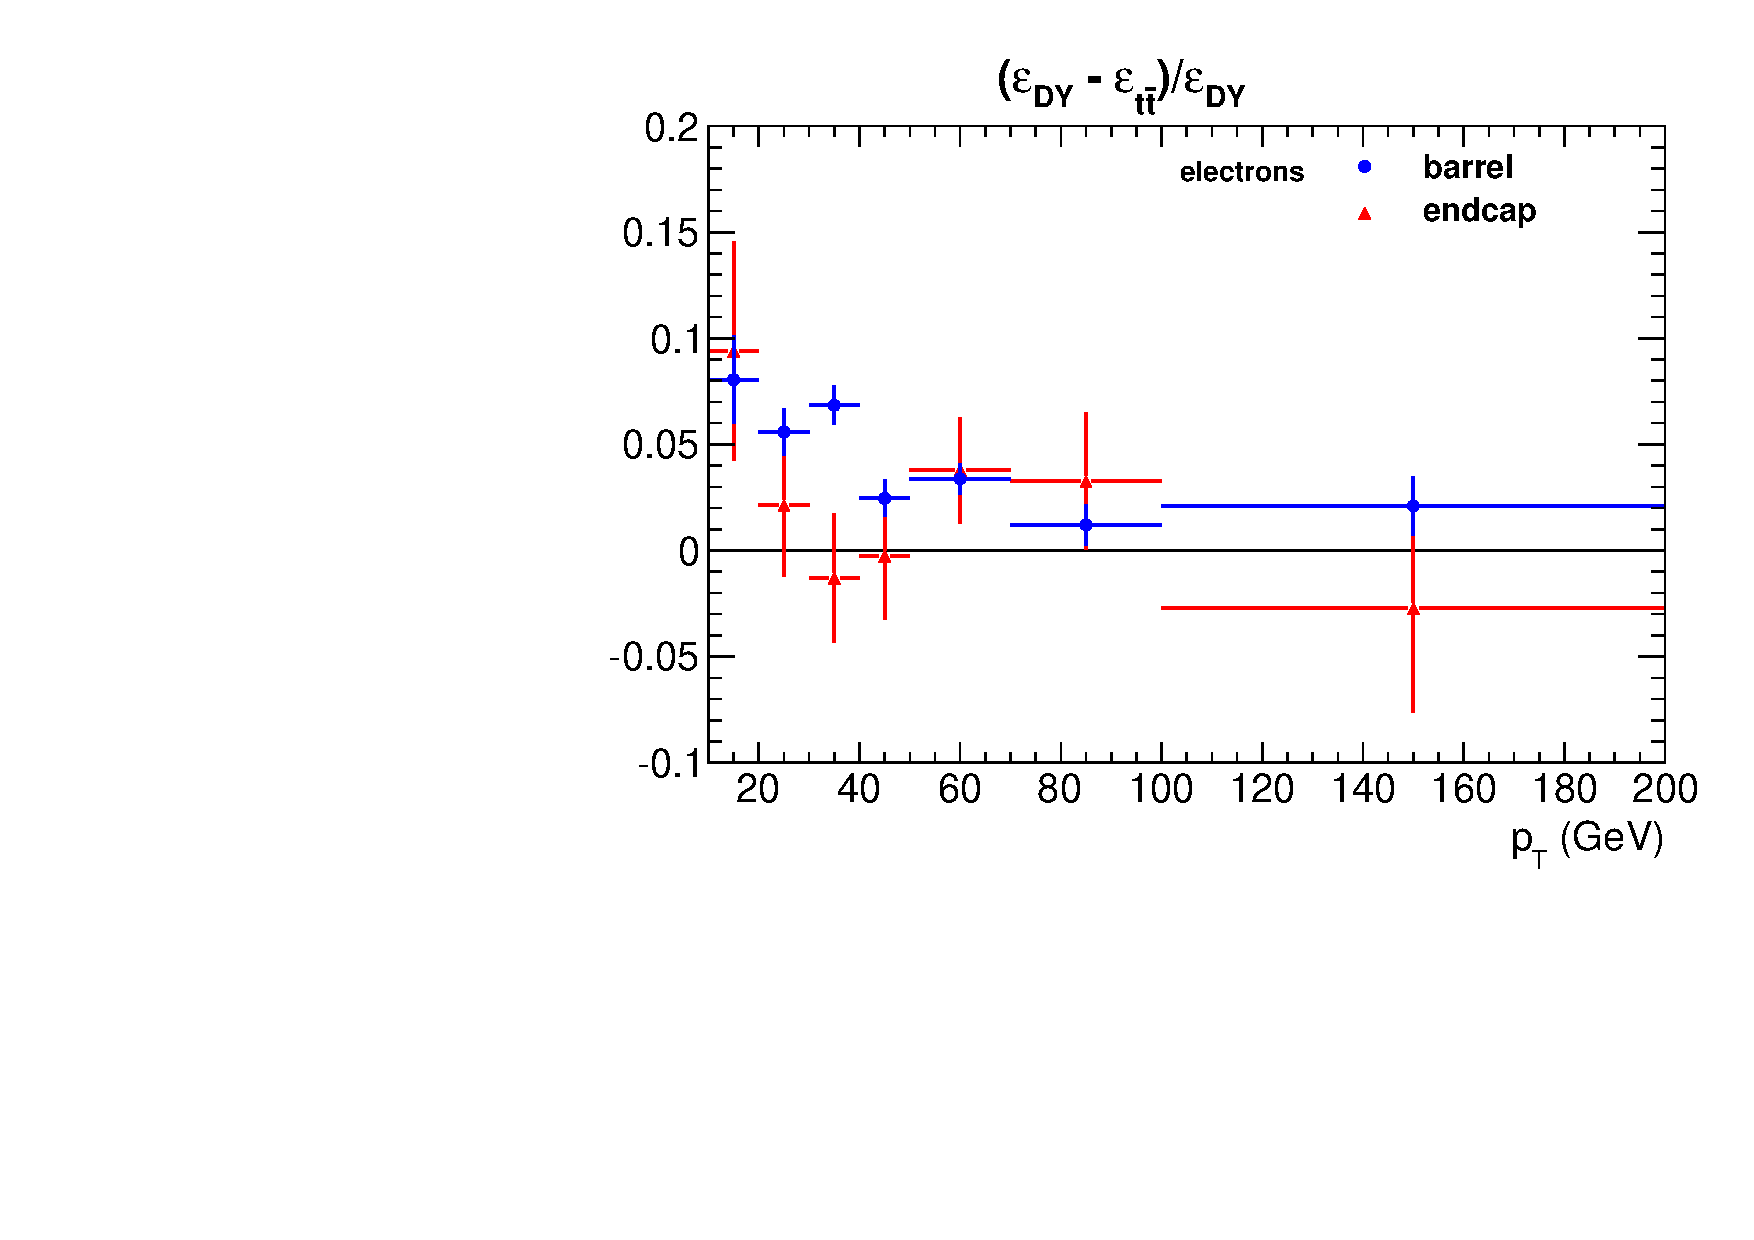
\includegraphics[width=0.49\linewidth]{p_eff_el_rel_diff_vs_pt_compare}
\includegraphics[width=0.49\linewidth]{p_eff_el_rel_diff_vs_eta}
\caption[The electron efficiency measured vs \pt~and \aeta]
{\label{fig:eff_comp_el}
The electron efficiency measured using DY (red) and \ttbar~MC (black). The
top two plots are the efficiencies projected vs \pt~and \aeta, respectively.
The bottom two plots are the relative differences between DY and \ttbar~ also
projected vs \pt~and \aeta.}
\end{center}
\end{figure}
% --------------------------------------------------------------------------- %
\begin{table}[!hbt]
\caption[The muon efficiency relative differences between DY and \ttbar]
{\label{tab:eff_comp_mu}
The muon efficiency relative differences between DY and \ttbar~
($(\epsilon_{DY} - \epsilon_{\ttbar})/\epsilon_{DY}$). The uncertainties are
statistical only.
}
\begin{center}
\begin{tabular}{c|c|c}
\hline\hline
\backslashbox{\pt}{\aeta} & 0.00 - 1.20       & 1.20 - 2.50       \\\hline
10 - 20 \GeV              & 0.113 $\pm$ 0.014 & 0.104 $\pm$ 0.016 \\
20 - 30 \GeV              & 0.109 $\pm$ 0.009 & 0.078 $\pm$ 0.012 \\
30 - 40 \GeV              & 0.084 $\pm$ 0.007 & 0.067 $\pm$ 0.011 \\
40 - 50 \GeV              & 0.075 $\pm$ 0.007 & 0.058 $\pm$ 0.011 \\
50 - 70 \GeV              & 0.047 $\pm$ 0.006 & 0.026 $\pm$ 0.009 \\
70 - 100 \GeV             & 0.036 $\pm$ 0.009 & 0.012 $\pm$ 0.013 \\
100- 200 \GeV             & 0.026 $\pm$ 0.014 & 0.042 $\pm$ 0.020 \\ \hline\hline
\end{tabular}
\end{center}
\end{table}
% --------------------------------------------------------------------------- %
\begin{figure}[!hbt]
\begin{center}
\includegraphics[width=0.49\linewidth]{p_eff_mu_vs_pt}
\includegraphics[width=0.49\linewidth]{p_eff_mu_vs_eta}
\includegraphics[width=0.49\linewidth]{p_eff_mu_rel_diff_vs_pt_compare}
\includegraphics[width=0.49\linewidth]{p_eff_mu_rel_diff_vs_eta}
\caption[The muon efficiency measured vs \pt~and \aeta]
{\label{fig:eff_comp_mu}
The muon efficiency measured using DY (red) and \ttbar~MC (black). The top two
plots are the efficiencies projected vs \pt~and \aeta, respectively. The bottom
two plots are the relative differences between DY and \ttbar~ also projected vs
\pt~and \aeta.
}
\end{center}
\end{figure}
 
% --------------------------------------------------------------------------- %
Here we see that the majority of the differences come at low \pt~where we
see relative differences on the order of 10\% for muons and 5\% for the
electrons. As we move to higher \pt~the differences are only on the order
of a few percent. To account for these differences we assign a systematic
uncertainty which is roughly half the relative difference stated in
tables~\ref{tab:eff_comp_el},~\ref{tab:eff_comp_mu}:
% --------------------------------------------------------------------------- %
\begin{itemize}
  \item muons: 5\% for $\pt < 30\ $\GeV~ and 3\% for $\pt > 30\ \GeV$
  \item electrons: 3\%
\end{itemize}

% --------------------------------------------------------------------------- %
To account for the differences in the efficiency between data and
simulation, the scale factors reported in Tables~\ref{tab:eff_comp_el}
and~\ref{tab:eff_comp_mu} are applied to each MC sample used in the prediction
with Table~\ref{tab:eff_lepsyst} summarizing the various systematic
uncertainties taken.
% --------------------------------------------------------------------------- %
\begin{table}[ht!]
\caption[The systematic uncertainties applied to the data-to-MC efficiency scale factors]
{\label{tab:eff_lepsyst}
The systematic uncertainties applied to the data-to-MC efficiency scale factors.
}
\begin{center}
\begin{tabular}{c|c|c|c}
\hline\hline
\multirow{3}{*}{\tnp}        & lepton flavor & $p_T < 15\ GeV$ & $p_T > 15\ GeV$ \\ \hline
                             & electron      & $10\%$          & $5\%$           \\
                             & muon          & $5\%$           & $3\%$           \\ \hline \hline
\multirow{3}{*}{composition} &               & $p_T < 30\ GeV$ & $p_T > 30\ GeV$ \\ \hline
                             & electron      & $3\%$           & $3\%$           \\
                             & muon          & $5\%$           & $3\%$           \\ \hline\hline
\end{tabular}
\end{center}
\end{table}
% --------------------------------------------------------------------------- %

% --------------------------------------------------------------------------- %
% --------------------------------------------------------------------------- %
\section{Trigger Efficiencies}
\label {sec:eff_trig}
% --------------------------------------------------------------------------- %
% --------------------------------------------------------------------------- %
The trigger efficiencies and data-to-MC scale factor is calculated for
every trigger and is applied \pt and \aeta dependent for each lepton.
Details on how the scale factors have been studied and calculated can be
found in~\cite{an_ufl2013}. The value of those scale factors is shown in
Table~\ref{tab:eff_trig}.
% --------------------------------------------------------------------------- %
\begin{table}[!hbt]
\begin{center}
\caption[Scale factors from trigger inefficiencies applied to Monte Carlo predictions from the rare backgrounds]
{\label{tab:eff_trig}
Scale factors from trigger inefficiencies applied to Monte Carlo predictions
from the \emph{irreducible} backgrounds. For some channels, scale factors are
parametrized by the trailing lepton \pt or \aeta.
}
\begin{tabular}{|l|c|l|c|} \hline\hline
Low-$\pt$            & Scale Factor & High-$\pt$           & Scale Factor  \\ \hline \hline
$\mu\mu$, $|\eta|<1$ & 0.94         & $\mu\mu$, $|\eta|<1$ & 0.90          \\ \hline
$\mu\mu$, $|\eta|>1$ & 0.90         & $\mu\mu$, $|\eta|>1$ & 0.81          \\ \hline
$e\mu$               & 0.93         & $e\mu$               & 0.93          \\ \hline
$ee$                 & 0.93         & $ee$, $\pt<30$       & 0.92          \\ \hline
                     &              & $ee$, $\pt>30$       & 0.96          \\ \hline\hline
\end{tabular}
\end{center}
\end{table}

% --------------------------------------------------------------------------- %
% --------------------------------------------------------------------------- %
\section{B-tagging Efficiency}
\label {sec:eff_btag}
% --------------------------------------------------------------------------- %
% --------------------------------------------------------------------------- %
Since the b-tagging efficiencies measured in data are somewhat different than
those measured by simulation, a scale factor is applied to simulated events to
take this difference into account. The CMS B-tagging and Vertex Group (BTV) has
measured the b-tagging scale factors between data and MC. The scale factors in
general depend on the jet flavor, \pt, and \aeta and the details are described
by the BTV in~\cite{beff_2012,btvtwiki}. These scale factors were measured on
muon-jet and \ttbar~ data and are documented in~\cite{btvtwiki}. In contrast to
the previous iterations of this analysis where the scale factor was applied as
an additional event weight, the scale factor will now be used to update the
b-tagging status on a jet-by-jet basis. A full description is provided in the
stated reference; however, we provide a short summary of the method here. In
this method, scale factors are used to update the b-tagging status on each jet
individually. In order to upgrade or downgrade the b-tagging status of each
individual jet, a random number generator is used. This gives the advantage
that the yields from MC can be treated the same way as data. The method in our
case is relatively simple since we only have one operating point. If $SF < 1$,
then the fraction of $f = 1 - SF$ b-tagged jets from the ``tagged'' collection
are to be downgraded to the ``non-tagged'' status and in this case, it is
not necessary to know the MC b-tagging efficiency. The situation gets more
complicated when $SF > 1$. It is necessary to upgrade the b-tagging status of
some of the untagged jets and the fraction of such jets that needs to be upgraded
is
% --------------------------------------------------------------------------- %
\[
  f = \frac{1 - SF}{1 - 1/\varepsilon_{MC}}.
\]
% --------------------------------------------------------------------------- %
Using this relationship and a random number, we recount the number of b-tagged
jets on all events and use the count of this new collection in all selections
regarding the \nbtags. To estimate the systematic uncertainty on the b-tagging
efficiency scale factor, the uncertainty is scaled up or down and then
the above procedure is repeated. The difference between the unscaled and
the scaled acceptance efficiency is used in determining the systematic
uncertainty. These are considered fully correlated between the search regions.
Figure~\ref{fig:eff_nbtags} shows the effect of the this rescaling procedure on the
\nbtags distribution on a \ttW MC sample which is required to pass the baseline
selections (SR0).
% --------------------------------------------------------------------------- %
\begin{figure}[!htb]
\begin{center}
\includegraphics[width=0.8\linewidth]{p_nbtags.pdf}
\end{center}
\caption[\nbtags~distribution for \ttW~MC sample to illustrate the effect of the b-tag rescaling procedure]
{\label{fig:eff_nbtags}
\nbtags~distribution for \ttW~MC sample to illustrate the effect of the b-tag
rescaling procedure on the number of b-tagged jets.
}
\end{figure}
% --------------------------------------------------------------------------- %

% --------------------------------------------------------------------------- %
% --------------------------------------------------------------------------- %
\chapter{Results}
\label {ch:results}
% --------------------------------------------------------------------------- %
% --------------------------------------------------------------------------- %
% captions for the SRs
% --------------------------------------------------------------------------- %
% --------------------------------------------------------------------------- %

% caption used for the exclusive yields
\newcommand{\exclcaption}{
compared to expectations from simulation alone, and from the data-driven
methods. The upper part of the table is based on simulation only and is used
only as a reference. The lower part is the main result of the analysis. The
SF (DF) contributions are for events with one (two) fake leptons. The {\em MC
Pred} contribution includes contributions from genuine same-sign lepton pairs
(a sum of the rows from \Wgamma down to the Higgs samples). The statistical
uncertainties on the MC contribution are calculated using the Clopper-Pearson
method. Systematic uncertainties (the second uncertainty if present) are
displayed only for the final combined type of background, no systematic
uncertainty is added for estimates with zero entries. Systematic uncertainties
are 100\% correlated among the channels.
}

% high pt
% --------------------------------------------------------------------------- %

\newcommand{\exclhptnamerZERO      } {{\bf Baseline with 0 btags (Signal Region 0): } Observed event yields in the \hpt~baseline                            } 
\newcommand{\exclhptnamerONE       } {{\bf Exclusive \hpt~Signal Region 1:       } Observed event yields in the low-\met, low-\Ht, and low-\njets~region    } 
\newcommand{\exclhptnamerTWO       } {{\bf Exclusive \hpt~Signal Region 2:       } Observed event yields in the low-\met, high-\Ht, and low-\njets~region   } 
\newcommand{\exclhptnamerTHREE     } {{\bf Exclusive \hpt~Signal Region 3:       } Observed event yields in the low-\met, low-\Ht, and high-\njets~region   } 
\newcommand{\exclhptnamerFOUR      } {{\bf Exclusive \hpt~Signal Region 4:       } Observed event yields in the low-\met, high-\Ht, and high-\njets~region  } 
\newcommand{\exclhptnamerFIVE      } {{\bf Exclusive \hpt~Signal Region 5:       } Observed event yields in the high-\met, low-\Ht, and low-\njets~region   } 
\newcommand{\exclhptnamerSIX       } {{\bf Exclusive \hpt~Signal Region 6:       } Observed event yields in the high-\met, high-\Ht, and low-\njets~region  } 
\newcommand{\exclhptnamerSEVEN     } {{\bf Exclusive \hpt~Signal Region 7:       } Observed event yields in the high-\met, low-\Ht, and high-\njets~region  } 
\newcommand{\exclhptnamerEIGHT     } {{\bf Exclusive \hpt~Signal Region 8:       } Observed event yields in the high-\met, high-\Ht, and high-\njets~region } 
\newcommand{\exclhptnamerONEZERO   } {{\bf Baseline with 1 btag (Signal Region 10): } Observed event yields in the \hpt~baseline                            } 
\newcommand{\exclhptnamerONEONE    } {{\bf Exclusive \hpt~Signal Region 11:      } Observed event yields in the low-\met, low-\Ht, and low-\njets~region    } 
\newcommand{\exclhptnamerONETWO    } {{\bf Exclusive \hpt~Signal Region 12:      } Observed event yields in the low-\met, high-\Ht, and low-\njets~region   } 
\newcommand{\exclhptnamerONETHREE  } {{\bf Exclusive \hpt~Signal Region 13:      } Observed event yields in the low-\met, low-\Ht, and high-\njets~region   } 
\newcommand{\exclhptnamerONEFOUR   } {{\bf Exclusive \hpt~Signal Region 14:      } Observed event yields in the low-\met, high-\Ht, and high-\njets~region  } 
\newcommand{\exclhptnamerONEFIVE   } {{\bf Exclusive \hpt~Signal Region 15:      } Observed event yields in the high-\met, low-\Ht, and low-\njets~region   } 
\newcommand{\exclhptnamerONESIX    } {{\bf Exclusive \hpt~Signal Region 16:      } Observed event yields in the high-\met, high-\Ht, and low-\njets~region  } 
\newcommand{\exclhptnamerONESEVEN  } {{\bf Exclusive \hpt~Signal Region 17:      } Observed event yields in the high-\met, low-\Ht, and high-\njets~region  } 
\newcommand{\exclhptnamerONEEIGHT  } {{\bf Exclusive \hpt~Signal Region 18:      } Observed event yields in the high-\met, high-\Ht, and high-\njets~region } 
\newcommand{\exclhptnamerTWOZERO   } {{\bf Baseline with 2 btag (Signal Region 20): } Observed event yields in the \hpt~baseline                            } 
\newcommand{\exclhptnamerTWOONE    } {{\bf Exclusive \hpt~Signal Region 21:      } Observed event yields in the low-\met, low-\Ht, and low-\njets~region    } 
\newcommand{\exclhptnamerTWOTWO    } {{\bf Exclusive \hpt~Signal Region 22:      } Observed event yields in the low-\met, high-\Ht, and low-\njets~region   } 
\newcommand{\exclhptnamerTWOTHREE  } {{\bf Exclusive \hpt~Signal Region 23:      } Observed event yields in the low-\met, low-\Ht, and high-\njets~region   } 
\newcommand{\exclhptnamerTWOFOUR   } {{\bf Exclusive \hpt~Signal Region 24:      } Observed event yields in the low-\met, high-\Ht, and high-\njets~region  } 
\newcommand{\exclhptnamerTWOFIVE   } {{\bf Exclusive \hpt~Signal Region 25:      } Observed event yields in the high-\met, low-\Ht, and low-\njets~region   } 
\newcommand{\exclhptnamerTWOSIX    } {{\bf Exclusive \hpt~Signal Region 26:      } Observed event yields in the high-\met, high-\Ht, and low-\njets~region  } 
\newcommand{\exclhptnamerTWOSEVEN  } {{\bf Exclusive \hpt~Signal Region 27:      } Observed event yields in the high-\met, low-\Ht, and high-\njets~region  } 
\newcommand{\exclhptnamerTWOEIGHT  } {{\bf Exclusive \hpt~Signal Region 28:      } Observed event yields in the high-\met, high-\Ht, and high-\njets~region } 
\newcommand{\exclhptnamerTHREEZERO } {{\bf High \pt~Signal Region 30:            } Observed event yields in the minimal region                              } 
\newcommand{\exclhptnamerTHREEONE  } {{\bf High \pt~Signal Region 31:            } Observed event yields in the minimal ``++'' region used for same-sign top} 
\newcommand{\exclhptnamerTHREETWO  } {{\bf High \pt~Signal Region 32:            } Observed event yields in the R-parity violation search region            } 
\newcommand{\exclhptnamerTHREETHREE} {{\bf High \pt~Signal Region 33:            } Observed event yields in the R-parity violation search region            } 
\newcommand{\exclhptnamerTHREEFOUR } {{\bf High \pt~Signal Region 34:            } Observed event yields in the minimal region                              } 
\newcommand{\exclhptnamerTHREEFIVE } {{\bf High \pt~Signal Region 35:            } Observed event yields in the minimal ``++'' region used for same-sign top} 

\newcommand{\exclhptcutsrZERO      } {(lepton \pt~$>$ 20/20 GeV, \Ht~$>$ 80 GeV, \met~$>$ 30 GeV if \Ht~$<$ 500 GeV (otherise no \met~cut), at least 2 jets with \pt~$>$ 40 GeV)                                           } 
\newcommand{\exclhptcutsrONE       } {($50\ \GeV < \met < 120\ \GeV$, $200\ \GeV < \Ht < 400\ \GeV$, between two and three jets with \pt~$>$ 40 GeV, and no b-tagged jets using CSVM)                                      } 
\newcommand{\exclhptcutsrTWO       } {($50\ \GeV < \met < 120\ \GeV$, $\Ht > 400\ \GeV$, between two and three jets with \pt~$>$ 40 GeV, and no b-tagged jets using CSVM)                                                  } 
\newcommand{\exclhptcutsrTHREE     } {($50\ \GeV < \met < 120\ \GeV$, $200\ \GeV < \Ht < 400\ \GeV$, greater than three jets with \pt~$>$ 40 GeV, and no b-tagged jets using CSVM)                                         } 
\newcommand{\exclhptcutsrFOUR      } {($50\ \GeV < \met < 120\ \GeV$, $\Ht > 400\ \GeV$, greater than three jets with \pt~$>$ 40 GeV, and no b-tagged jets using CSVM)                                                     } 
\newcommand{\exclhptcutsrFIVE      } {($\met > 120\ \GeV$, $200\ \GeV < \Ht < 400\ \GeV$, between two and three jets with \pt~$>$ 40 GeV, and no b-tagged jets using CSVM)                                                 } 
\newcommand{\exclhptcutsrSIX       } {($\met > 120\ \GeV$, $\Ht > 400\ \GeV$, between two and three jets with \pt~$>$ 40 GeV, and no b-tagged jets using CSVM)                                                             } 
\newcommand{\exclhptcutsrSEVEN     } {($\met > 120\ \GeV$, $200\ \GeV < \Ht < 400\ \GeV$, greater than three jets with \pt~$>$ 40 GeV, and no b-tagged jets using CSVM)                                                    } 
\newcommand{\exclhptcutsrEIGHT     } {($\met > 120\ \GeV$, $\Ht > 400\ \GeV$, greater than three jets with \pt~$>$ 40 GeV)                                                                                                 } 
\newcommand{\exclhptcutsrONEZERO   } {(lepton \pt~$>$ 20/20 GeV, \Ht~$>$ 80 GeV, \met~$>$ 30 GeV if \Ht~$<$ 500 GeV (otherise no \met~cut), at least 2 jets with \pt~$>$ 40 GeV and exactly one b-tagged jet using CSVM)   } 
\newcommand{\exclhptcutsrONEONE    } {($50\ \GeV < \met < 120\ \GeV$, $200\ \GeV < \Ht < 400\ \GeV$, between two and three jets with \pt~$>$ 40 GeV and exactly one b-tagged jet using CSVM)                               } 
\newcommand{\exclhptcutsrONETWO    } {($50\ \GeV < \met < 120\ \GeV$, $\Ht > 400\ \GeV$, between two and three jets with \pt~$>$ 40 GeV and exactly one b-tagged jet using CSVM)                                           } 
\newcommand{\exclhptcutsrONETHREE  } {($50\ \GeV < \met < 120\ \GeV$, $200\ \GeV < \Ht < 400\ \GeV$, greater than three jets with \pt~$>$ 40 GeV and exactly one b-tagged jet using CSVM)                                  } 
\newcommand{\exclhptcutsrONEFOUR   } {($50\ \GeV < \met < 120\ \GeV$, $\Ht > 400\ \GeV$, greater than three jets with \pt~$>$ 40 GeV and exactly one b-tagged jet using CSVM)                                              } 
\newcommand{\exclhptcutsrONEFIVE   } {($\met > 120\ \GeV$, $200\ \GeV < \Ht < 400\ \GeV$, between two and three jets with \pt~$>$ 40 GeV and exactly one b-tagged jet using CSVM)                                          } 
\newcommand{\exclhptcutsrONESIX    } {($\met > 120\ \GeV$, $\Ht > 400\ \GeV$, between two and three jets with \pt~$>$ 40 GeV and exactly one b-tagged jet using CSVM)                                                      } 
\newcommand{\exclhptcutsrONESEVEN  } {($\met > 120\ \GeV$, $200\ \GeV < \Ht < 400\ \GeV$, greater than three jets with \pt~$>$ 40 GeV and exactly one b-tagged jet using CSVM)                                             } 
\newcommand{\exclhptcutsrONEEIGHT  } {($\met > 120\ \GeV$, $\Ht > 400\ \GeV$, greater than three jets with \pt~$>$ 40 GeV and exactly one b-tagged jet using CSVM)                                                         } 
\newcommand{\exclhptcutsrTWOZERO   } {(lepton \pt~$>$ 20/20 GeV, \Ht~$>$ 80 GeV, \met~$>$ 30 GeV if \Ht~$<$ 500 GeV (otherise no \met~cut), at least 2 jets with \pt~$>$ 40 GeV and at least two b-tagged jets using CSVM) } 
\newcommand{\exclhptcutsrTWOONE    } {($50\ \GeV < \met < 120\ \GeV$, $200\ \GeV < \Ht < 400\ \GeV$, between two and three jets with \pt~$>$ 40 GeV and at least two b-tagged jets using CSVM)                             } 
\newcommand{\exclhptcutsrTWOTWO    } {($50\ \GeV < \met < 120\ \GeV$, $\Ht > 400\ \GeV$, between two and three jets with \pt~$>$ 40 GeV and at least two b-tagged jets using CSVM)                                         } 
\newcommand{\exclhptcutsrTWOTHREE  } {($50\ \GeV < \met < 120\ \GeV$, $200\ \GeV < \Ht < 400\ \GeV$, greater than three jets with \pt~$>$ 40 GeV and at least two b-tagged jets using CSVM)                                } 
\newcommand{\exclhptcutsrTWOFOUR   } {($50\ \GeV < \met < 120\ \GeV$, $\Ht > 400\ \GeV$, greater than three jets with \pt~$>$ 40 GeV and at least two b-tagged jets using CSVM)                                            } 
\newcommand{\exclhptcutsrTWOFIVE   } {($\met > 120\ \GeV$, $200\ \GeV < \Ht < 400\ \GeV$, between two and three jets with \pt~$>$ 40 GeV and at least two b-tagged jets using CSVM)                                        } 
\newcommand{\exclhptcutsrTWOSIX    } {($\met > 120\ \GeV$, $\Ht > 400\ \GeV$, between two and three jets with \pt~$>$ 40 GeV and at least two b-tagged jets using CSVM)                                                    } 
\newcommand{\exclhptcutsrTWOSEVEN  } {($\met > 120\ \GeV$, $200\ \GeV < \Ht < 400\ \GeV$, greater than three jets with \pt~$>$ 40 GeV and at least two b-tagged jets using CSVM)                                           } 
\newcommand{\exclhptcutsrTWOEIGHT  } {($\met > 120\ \GeV$, $\Ht > 400\ \GeV$, greater than three jets with \pt~$>$ 40 GeV and at least two b-tagged jets using CSVM)                                                       } 
\newcommand{\exclhptcutsrTHREEZERO } {($\met > 30\ \GeV$, at least two jets with \pt~$>$ 40 GeV and at least two b-tagged jets using CSVM)                                                                                 } 
\newcommand{\exclhptcutsrTHREEONE  } {($\met > 30\ \GeV$, dilepton charge is ``++'', at least two jets with \pt~$>$ 40 GeV and at least two b-tagged jets using CSVM)                                                      } 
\newcommand{\exclhptcutsrTHREETWO  } {($\Ht > 500\ \GeV$, at least two jets with \pt~$>$ 40 GeV and no requirement on the number of b-tagged jets                                                                          } 
\newcommand{\exclhptcutsrTHREETHREE} {($\Ht > 500\ \GeV$, at least two jets with \pt~$>$ 40 GeV and at least two b-tagged jets using CSVM)                                                                                 } 
\newcommand{\exclhptcutsrTHREEFOUR } {($\met > 30\ \GeV$, at least two jets with \pt~$>$ 40 GeV and exactly one b-tagged jets using CSVM)                                                                                  } 
\newcommand{\exclhptcutsrTHREEFIVE } {($\met > 30\ \GeV$, dilepton charge is ``++'', at least two jets with \pt~$>$ 40 GeV and exactly one b-tagged jets using CSVM)                                                       } 

% \begin{table}[h] \begin{center} {\footnotesize \begin{tabular}{l|cccc} \hline\hline
source & $ee$ & $\mu\mu$ & $e\mu$ & $\ell\ell $ \\
\hline
$t\overline{t} \rightarrow \ell \ell X$ &  6.40 $\pm$  2.90 &  0.00 $\pm$  1.21 &  5.81 $\pm$  2.80 & 12.21 $\pm$  3.71 \\
$t\overline{t} \rightarrow \ell (b \rightarrow \ell) X$ & 13.86 $\pm$  3.98 & 10.25 $\pm$  3.56 & 22.25 $\pm$  4.78 & 46.36 $\pm$  6.65 \\
$t\overline{t} \rightarrow \ell (\slashed b \rightarrow \ell) X$ &  3.47 $\pm$  2.35 &  0.51 $\pm$  1.51 &  6.95 $\pm$  2.99 & 10.93 $\pm$  3.56 \\
        $t\overline{t}\ \rm{other}$ &  0.00 $\pm$  1.21 &  0.00 $\pm$  1.21 &  0.00 $\pm$  1.21 &  0.00 $\pm$  1.21 \\
\hline
                       t, s-channel &  0.00 $\pm$  0.52 &  0.00 $\pm$  0.52 &  0.00 $\pm$  0.52 &  0.00 $\pm$  0.52 \\
                       t, t-channel &  0.27 $\pm$  0.68 &  0.75 $\pm$  0.86 &  1.55 $\pm$  1.05 &  2.56 $\pm$  1.25 \\
                                 tW &  0.76 $\pm$  1.14 &  0.71 $\pm$  1.14 &  2.26 $\pm$  1.55 &  3.72 $\pm$  1.85 \\
\hline
         $DY \rightarrow \ell \ell$ & 18.03 $\pm$  9.25 &  0.00 $\pm$  4.14 &  5.81 $\pm$  6.57 & 23.85 $\pm$ 10.26 \\
      $W+jets \rightarrow \ell \nu$ &  0.00 $\pm$ 73.20 &  0.00 $\pm$ 73.20 &  0.00 $\pm$ 73.20 &  0.00 $\pm$ 73.20 \\
                                 WW &  0.00 $\pm$  0.11 &  0.00 $\pm$  0.11 &  0.00 $\pm$  0.11 &  0.00 $\pm$  0.11 \\
\hline
$W\gamma^{*} \rightarrow \ell \nu \mu\mu$ &  0.00 $\pm$  0.23 &  0.20 $\pm$  0.33 &  0.22 $\pm$  0.33 &  0.42 $\pm$  0.39 \\
$W\gamma^{*} \rightarrow \ell \nu \tau\tau$ &  0.11 $\pm$  0.30 &  0.22 $\pm$  0.34 &  0.00 $\pm$  0.24 &  0.33 $\pm$  0.38 \\
                                 WZ & 18.53 $\pm$  0.47 & 17.10 $\pm$  0.47 & 36.72 $\pm$  0.66 & 72.35 $\pm$  0.93 \\
                                 ZZ &  1.19 $\pm$  0.03 &  0.90 $\pm$  0.03 &  2.22 $\pm$  0.04 &  4.31 $\pm$  0.06 \\
\hline
              $t\overline{t}\gamma$ &  0.53 $\pm$  1.35 &  0.00 $\pm$  1.08 &  3.07 $\pm$  2.10 &  3.60 $\pm$  2.21 \\
                   $t\overline{t}W$ & 10.61 $\pm$  0.55 & 14.72 $\pm$  0.66 & 26.55 $\pm$  0.85 & 51.88 $\pm$  1.19 \\
                   $t\overline{t}Z$ &  2.80 $\pm$  0.26 &  3.16 $\pm$  0.29 &  6.25 $\pm$  0.39 & 12.20 $\pm$  0.54 \\
    $tbZ (Z \rightarrow \ell \ell)$ &  0.44 $\pm$  0.03 &  0.34 $\pm$  0.03 &  0.82 $\pm$  0.04 &  1.59 $\pm$  0.05 \\
                  $t\overline{t}WW$ &  0.22 $\pm$  0.01 &  0.29 $\pm$  0.01 &  0.51 $\pm$  0.01 &  1.01 $\pm$  0.01 \\
                         $WW\gamma$ &  0.00 $\pm$  0.09 &  0.00 $\pm$  0.09 &  0.00 $\pm$  0.09 &  0.00 $\pm$  0.09 \\
                                WWW &  1.84 $\pm$  0.13 &  2.44 $\pm$  0.15 &  4.17 $\pm$  0.19 &  8.45 $\pm$  0.27 \\
                                WWZ &  0.40 $\pm$  0.05 &  0.32 $\pm$  0.05 &  0.80 $\pm$  0.07 &  1.52 $\pm$  0.10 \\
                                WZZ &  0.08 $\pm$  0.01 &  0.08 $\pm$  0.01 &  0.19 $\pm$  0.02 &  0.36 $\pm$  0.03 \\
                                ZZZ &  0.01 $\pm$  0.00 &  0.00 $\pm$  0.00 &  0.01 $\pm$  0.00 &  0.02 $\pm$  0.00 \\
                 $qqW^{\pm}W^{\pm}$ &  8.07 $\pm$  0.66 & 11.04 $\pm$  0.79 & 20.11 $\pm$  1.01 & 39.22 $\pm$  1.40 \\
                            WW(DPS) &  0.10 $\pm$  0.06 &  0.19 $\pm$  0.07 &  0.31 $\pm$  0.08 &  0.60 $\pm$  0.11 \\
WH, ZH, $t\bar{t}H$; $H \rightarrow WW$ &  2.72 $\pm$  0.31 &  2.97 $\pm$  0.33 &  5.94 $\pm$  0.44 & 11.63 $\pm$  0.61 \\
WH, ZH, $t\bar{t}H$; $H \rightarrow ZZ$ &  0.12 $\pm$  0.01 &  0.15 $\pm$  0.02 &  0.29 $\pm$  0.02 &  0.55 $\pm$  0.03 \\
WH, ZH, $t\bar{t}H$; $H \rightarrow \tau\tau$ &  0.40 $\pm$  0.04 &  0.44 $\pm$  0.05 &  0.74 $\pm$  0.06 &  1.58 $\pm$  0.08 \\
\hline\hline
                           Total MC & 90.94 $\pm$ 74.03 & 66.77 $\pm$ 73.48 & 153.54 $\pm$ 73.85 & 311.24 $\pm$ 74.51 \\
\hline
                                 SF & 90.86 $\pm$  8.69 & 92.64 $\pm$  5.45 & 200.91 $\pm$ 11.00 & 384.41 $\pm$ 15.04 \\
                                 DF &  5.89 $\pm$  0.48 &  4.09 $\pm$  0.29 &  9.72 $\pm$  0.55 & 19.69 $\pm$  0.79 \\
                                 SC &  2.30 $\pm$  0.53 &  2.24 $\pm$  0.50 &  4.59 $\pm$  1.04 &  9.14 $\pm$  2.00 \\
                            SF + DF & 96.75 $\pm$  8.65 & 96.73 $\pm$  5.43 & 210.62 $\pm$ 10.96 & 404.10 $\pm$ 14.98 \\
\hline
                       SF + DF - SC & 94.44 $\pm$  8.66 $\pm$ 47.22 & 94.49 $\pm$  5.45 $\pm$ 47.24 & 206.03 $\pm$ 11.01 $\pm$ 103.02 & 394.96 $\pm$ 15.11 $\pm$ 197.48 \\
\hline\hline
                       Charge Flips & 23.44 $\pm$  1.16 $\pm$  7.03 &  0.00 $\pm$  0.00 $\pm$  0.00 &  5.22 $\pm$  0.45 $\pm$  1.57 & 28.66 $\pm$  1.24 $\pm$  8.60 \\
\hline
                            MC Pred & 48.15 $\pm$  1.77 $\pm$ 24.08 & 54.56 $\pm$  1.71 $\pm$ 27.28 & 108.91 $\pm$  2.68 $\pm$ 54.46 & 211.62 $\pm$  3.20 $\pm$ 105.81 \\
\hline
                         Total Pred & 166.04 $\pm$  8.92 $\pm$ 53.47 & 149.04 $\pm$  5.71 $\pm$ 54.55 & 320.17 $\pm$ 11.34 $\pm$ 116.53 & 635.24 $\pm$ 15.50 $\pm$ 224.21 \\
\hline\hline
                               Data &   146 &   111 &   220 &   477 \\
\hline\hline
\end{tabular}

} \end{center} \caption{\label{tab:yield_excl_hpt_sr0} \exclhptnamerZERO       \exclhptcutsrZERO       \exclcaption} \end{table} \clearpage
% \begin{table}[h] \begin{center} {\footnotesize \begin{tabular}{l|cccc} \hline\hline
source & $ee$ & $\mu\mu$ & $e\mu$ & $\ell\ell $ \\
\hline
$t\overline{t} \rightarrow \ell \ell X$ &  0.61 $\pm$  1.51 &  0.00 $\pm$  1.21 &  0.60 $\pm$  1.51 &  1.21 $\pm$  1.73 \\
$t\overline{t} \rightarrow \ell (b \rightarrow \ell) X$ &  2.21 $\pm$  2.07 &  0.00 $\pm$  1.21 &  1.70 $\pm$  1.91 &  3.91 $\pm$  2.47 \\
$t\overline{t} \rightarrow \ell (\slashed b \rightarrow \ell) X$ &  0.00 $\pm$  1.21 &  0.00 $\pm$  1.21 &  0.00 $\pm$  1.21 &  0.00 $\pm$  1.21 \\
        $t\overline{t}\ \rm{other}$ &  0.00 $\pm$  1.21 &  0.00 $\pm$  1.21 &  0.00 $\pm$  1.21 &  0.00 $\pm$  1.21 \\
\hline
                       t, s-channel &  0.00 $\pm$  0.52 &  0.00 $\pm$  0.52 &  0.00 $\pm$  0.52 &  0.00 $\pm$  0.52 \\
                       t, t-channel &  0.00 $\pm$  0.54 &  0.00 $\pm$  0.54 &  0.00 $\pm$  0.54 &  0.00 $\pm$  0.54 \\
                                 tW &  0.39 $\pm$  1.00 &  0.00 $\pm$  0.80 &  0.00 $\pm$  0.80 &  0.39 $\pm$  1.00 \\
\hline
         $DY \rightarrow \ell \ell$ &  2.07 $\pm$  5.18 &  0.00 $\pm$  4.14 &  0.00 $\pm$  4.14 &  2.07 $\pm$  5.18 \\
      $W+jets \rightarrow \ell \nu$ &  0.00 $\pm$ 73.20 &  0.00 $\pm$ 73.20 &  0.00 $\pm$ 73.20 &  0.00 $\pm$ 73.20 \\
                                 WW &  0.00 $\pm$  0.11 &  0.00 $\pm$  0.11 &  0.00 $\pm$  0.11 &  0.00 $\pm$  0.11 \\
\hline
$W\gamma^{*} \rightarrow \ell \nu \mu\mu$ &  0.00 $\pm$  0.23 &  0.00 $\pm$  0.23 &  0.00 $\pm$  0.23 &  0.00 $\pm$  0.23 \\
$W\gamma^{*} \rightarrow \ell \nu \tau\tau$ &  0.00 $\pm$  0.24 &  0.00 $\pm$  0.24 &  0.00 $\pm$  0.24 &  0.00 $\pm$  0.24 \\
                                 WZ &  2.92 $\pm$  0.19 &  2.62 $\pm$  0.19 &  6.39 $\pm$  0.28 & 11.93 $\pm$  0.39 \\
                                 ZZ &  0.12 $\pm$  0.01 &  0.11 $\pm$  0.01 &  0.24 $\pm$  0.01 &  0.47 $\pm$  0.02 \\
\hline
              $t\overline{t}\gamma$ &  0.10 $\pm$  0.24 &  0.00 $\pm$  1.08 &  0.56 $\pm$  0.38 &  0.65 $\pm$  0.40 \\
                   $t\overline{t}W$ &  0.37 $\pm$  0.12 &  0.64 $\pm$  0.16 &  1.07 $\pm$  0.19 &  2.08 $\pm$  0.26 \\
                   $t\overline{t}Z$ &  0.15 $\pm$  0.08 &  0.13 $\pm$  0.07 &  0.32 $\pm$  0.10 &  0.59 $\pm$  0.13 \\
    $tbZ (Z \rightarrow \ell \ell)$ &  0.04 $\pm$  0.01 &  0.02 $\pm$  0.01 &  0.07 $\pm$  0.01 &  0.13 $\pm$  0.02 \\
                  $t\overline{t}WW$ &  0.01 $\pm$  0.00 &  0.01 $\pm$  0.00 &  0.02 $\pm$  0.00 &  0.03 $\pm$  0.00 \\
                         $WW\gamma$ &  0.00 $\pm$  0.09 &  0.00 $\pm$  0.09 &  0.00 $\pm$  0.09 &  0.00 $\pm$  0.09 \\
                                WWW &  0.33 $\pm$  0.06 &  0.34 $\pm$  0.06 &  0.58 $\pm$  0.08 &  1.25 $\pm$  0.11 \\
                                WWZ &  0.06 $\pm$  0.02 &  0.04 $\pm$  0.02 &  0.08 $\pm$  0.03 &  0.18 $\pm$  0.04 \\
                                WZZ &  0.01 $\pm$  0.01 &  0.01 $\pm$  0.01 &  0.03 $\pm$  0.01 &  0.05 $\pm$  0.01 \\
                                ZZZ &  0.00 $\pm$  0.00 &  0.00 $\pm$  0.00 &  0.00 $\pm$  0.00 &  0.00 $\pm$  0.00 \\
                 $qqW^{\pm}W^{\pm}$ &  1.48 $\pm$  0.32 &  1.96 $\pm$  0.36 &  4.26 $\pm$  0.48 &  7.70 $\pm$  0.64 \\
                            WW(DPS) &  0.00 $\pm$  0.03 &  0.02 $\pm$  0.04 &  0.01 $\pm$  0.03 &  0.03 $\pm$  0.04 \\
WH, ZH, $t\bar{t}H$; $H \rightarrow WW$ &  0.09 $\pm$  0.08 &  0.25 $\pm$  0.11 &  0.24 $\pm$  0.11 &  0.58 $\pm$  0.16 \\
WH, ZH, $t\bar{t}H$; $H \rightarrow ZZ$ &  0.01 $\pm$  0.00 &  0.01 $\pm$  0.01 &  0.02 $\pm$  0.01 &  0.05 $\pm$  0.01 \\
WH, ZH, $t\bar{t}H$; $H \rightarrow \tau\tau$ &  0.03 $\pm$  0.02 &  0.02 $\pm$  0.01 &  0.07 $\pm$  0.02 &  0.13 $\pm$  0.03 \\
\hline\hline
                           Total MC & 10.99 $\pm$ 73.46 &  6.19 $\pm$ 73.38 & 16.24 $\pm$ 73.39 & 33.41 $\pm$ 73.49 \\
\hline
                                 SF &  6.70 $\pm$  1.33 &  6.14 $\pm$  0.97 & 15.38 $\pm$  1.83 & 28.23 $\pm$  2.46 \\
                                 DF &  0.35 $\pm$  0.10 &  0.24 $\pm$  0.06 &  0.92 $\pm$  0.15 &  1.51 $\pm$  0.19 \\
                                 SC &  0.32 $\pm$  0.09 &  0.29 $\pm$  0.08 &  0.50 $\pm$  0.13 &  1.11 $\pm$  0.28 \\
                            SF + DF &  7.05 $\pm$  1.31 &  6.38 $\pm$  0.97 & 16.30 $\pm$  1.82 & 29.73 $\pm$  2.44 \\
\hline
                       SF + DF - SC &  6.73 $\pm$  1.32 $\pm$  3.37 &  6.09 $\pm$  0.97 $\pm$  3.04 & 15.80 $\pm$  1.82 $\pm$  7.90 & 28.62 $\pm$  2.46 $\pm$ 14.31 \\
\hline\hline
                       Charge Flips &  1.31 $\pm$  0.09 $\pm$  0.39 &  0.00 $\pm$  0.00 $\pm$  0.00 &  0.25 $\pm$  0.03 $\pm$  0.08 &  1.56 $\pm$  0.10 $\pm$  0.47 \\
\hline
                            MC Pred &  5.71 $\pm$  0.59 $\pm$  2.86 &  6.19 $\pm$  1.23 $\pm$  3.09 & 13.94 $\pm$  0.80 $\pm$  6.97 & 25.84 $\pm$  0.98 $\pm$ 12.92 \\
\hline
                         Total Pred & 13.76 $\pm$  1.45 $\pm$  4.43 & 12.27 $\pm$  1.56 $\pm$  4.34 & 29.99 $\pm$  1.99 $\pm$ 10.54 & 56.02 $\pm$  2.65 $\pm$ 19.28 \\
\hline\hline
                               Data &    15 &    11 &    22 &    48 \\
\hline\hline
\end{tabular}

} \end{center} \caption{\label{tab:yield_excl_hpt_sr1 } \exclhptnamerONE        \exclhptcutsrONE        \exclcaption} \end{table} \clearpage
% \begin{table}[h] \begin{center} {\footnotesize \begin{tabular}{l|cccc} \hline\hline
source & $ee$ & $\mu\mu$ & $e\mu$ & $\ell\ell $ \\
\hline
$t\overline{t} \rightarrow \ell \ell X$ &  0.00 $\pm$  1.21 &  0.00 $\pm$  1.21 &  0.00 $\pm$  1.21 &  0.00 $\pm$  1.21 \\
$t\overline{t} \rightarrow \ell (b \rightarrow \ell) X$ &  0.00 $\pm$  1.21 &  0.00 $\pm$  1.21 &  0.00 $\pm$  1.21 &  0.00 $\pm$  1.21 \\
$t\overline{t} \rightarrow \ell (\slashed b \rightarrow \ell) X$ &  0.00 $\pm$  1.21 &  0.00 $\pm$  1.21 &  0.00 $\pm$  1.21 &  0.00 $\pm$  1.21 \\
        $t\overline{t}\ \rm{other}$ &  0.00 $\pm$  1.21 &  0.00 $\pm$  1.21 &  0.00 $\pm$  1.21 &  0.00 $\pm$  1.21 \\
\hline
                       t, s-channel &  0.00 $\pm$  0.52 &  0.00 $\pm$  0.52 &  0.00 $\pm$  0.52 &  0.00 $\pm$  0.52 \\
                       t, t-channel &  0.00 $\pm$  0.54 &  0.00 $\pm$  0.54 &  0.00 $\pm$  0.54 &  0.00 $\pm$  0.54 \\
                                 tW &  0.00 $\pm$  0.80 &  0.00 $\pm$  0.80 &  0.00 $\pm$  0.80 &  0.00 $\pm$  0.80 \\
\hline
         $DY \rightarrow \ell \ell$ &  0.00 $\pm$  4.14 &  0.00 $\pm$  4.14 &  0.00 $\pm$  4.14 &  0.00 $\pm$  4.14 \\
      $W+jets \rightarrow \ell \nu$ &  0.00 $\pm$ 73.20 &  0.00 $\pm$ 73.20 &  0.00 $\pm$ 73.20 &  0.00 $\pm$ 73.20 \\
                                 WW &  0.00 $\pm$  0.11 &  0.00 $\pm$  0.11 &  0.00 $\pm$  0.11 &  0.00 $\pm$  0.11 \\
\hline
$W\gamma^{*} \rightarrow \ell \nu \mu\mu$ &  0.00 $\pm$  0.23 &  0.00 $\pm$  0.23 &  0.00 $\pm$  0.23 &  0.00 $\pm$  0.23 \\
$W\gamma^{*} \rightarrow \ell \nu \tau\tau$ &  0.00 $\pm$  0.24 &  0.00 $\pm$  0.24 &  0.00 $\pm$  0.24 &  0.00 $\pm$  0.24 \\
                                 WZ &  0.50 $\pm$  0.09 &  0.57 $\pm$  0.10 &  1.06 $\pm$  0.12 &  2.13 $\pm$  0.17 \\
                                 ZZ &  0.02 $\pm$  0.01 &  0.02 $\pm$  0.01 &  0.05 $\pm$  0.01 &  0.09 $\pm$  0.01 \\
\hline
              $t\overline{t}\gamma$ &  0.01 $\pm$  0.02 &  0.00 $\pm$  1.08 &  0.05 $\pm$  0.03 &  0.05 $\pm$  0.03 \\
                   $t\overline{t}W$ &  0.04 $\pm$  0.06 &  0.11 $\pm$  0.08 &  0.20 $\pm$  0.10 &  0.36 $\pm$  0.12 \\
                   $t\overline{t}Z$ &  0.02 $\pm$  0.04 &  0.01 $\pm$  0.04 &  0.07 $\pm$  0.06 &  0.10 $\pm$  0.07 \\
    $tbZ (Z \rightarrow \ell \ell)$ &  0.01 $\pm$  0.01 &  0.01 $\pm$  0.01 &  0.01 $\pm$  0.01 &  0.02 $\pm$  0.01 \\
                  $t\overline{t}WW$ &  0.00 $\pm$  0.00 &  0.00 $\pm$  0.00 &  0.00 $\pm$  0.00 &  0.01 $\pm$  0.00 \\
                         $WW\gamma$ &  0.00 $\pm$  0.09 &  0.00 $\pm$  0.09 &  0.00 $\pm$  0.09 &  0.00 $\pm$  0.09 \\
                                WWW &  0.08 $\pm$  0.03 &  0.16 $\pm$  0.05 &  0.20 $\pm$  0.05 &  0.44 $\pm$  0.07 \\
                                WWZ &  0.02 $\pm$  0.02 &  0.01 $\pm$  0.01 &  0.04 $\pm$  0.02 &  0.07 $\pm$  0.03 \\
                                WZZ &  0.00 $\pm$  0.00 &  0.00 $\pm$  0.00 &  0.01 $\pm$  0.01 &  0.01 $\pm$  0.01 \\
                                ZZZ &  0.00 $\pm$  0.00 &  0.00 $\pm$  0.00 &  0.00 $\pm$  0.00 &  0.00 $\pm$  0.00 \\
                 $qqW^{\pm}W^{\pm}$ &  0.50 $\pm$  0.20 &  0.71 $\pm$  0.25 &  1.73 $\pm$  0.34 &  2.94 $\pm$  0.43 \\
                            WW(DPS) &  0.00 $\pm$  0.03 &  0.00 $\pm$  0.03 &  0.00 $\pm$  0.03 &  0.00 $\pm$  0.03 \\
WH, ZH, $t\bar{t}H$; $H \rightarrow WW$ &  0.00 $\pm$  0.05 &  0.02 $\pm$  0.06 &  0.04 $\pm$  0.07 &  0.06 $\pm$  0.07 \\
WH, ZH, $t\bar{t}H$; $H \rightarrow ZZ$ &  0.00 $\pm$  0.00 &  0.00 $\pm$  0.00 &  0.00 $\pm$  0.00 &  0.00 $\pm$  0.00 \\
WH, ZH, $t\bar{t}H$; $H \rightarrow \tau\tau$ &  0.01 $\pm$  0.01 &  0.00 $\pm$  0.01 &  0.01 $\pm$  0.01 &  0.01 $\pm$  0.01 \\
\hline\hline
                           Total MC &  1.20 $\pm$ 73.37 &  1.64 $\pm$ 73.38 &  3.46 $\pm$ 73.37 &  6.30 $\pm$ 73.37 \\
\hline
                                 SF &  1.21 $\pm$  0.47 &  0.58 $\pm$  0.29 &  1.27 $\pm$  0.44 &  3.07 $\pm$  0.71 \\
                                 DF &  0.03 $\pm$  0.03 &  0.05 $\pm$  0.03 &  0.03 $\pm$  0.02 &  0.12 $\pm$  0.05 \\
                                 SC &  0.06 $\pm$  0.02 &  0.06 $\pm$  0.02 &  0.12 $\pm$  0.04 &  0.24 $\pm$  0.07 \\
                            SF + DF &  1.24 $\pm$  0.46 &  0.64 $\pm$  0.29 &  1.31 $\pm$  0.44 &  3.18 $\pm$  0.70 \\
\hline
                       SF + DF - SC &  1.18 $\pm$  0.47 $\pm$  0.59 &  0.58 $\pm$  0.29 $\pm$  0.29 &  1.18 $\pm$  0.44 $\pm$  0.59 &  2.94 $\pm$  0.71 $\pm$  1.47 \\
\hline\hline
                       Charge Flips &  0.34 $\pm$  0.04 $\pm$  0.10 &  0.00 $\pm$  0.00 $\pm$  0.00 &  0.03 $\pm$  0.01 $\pm$  0.01 &  0.37 $\pm$  0.04 $\pm$  0.11 \\
\hline
                            MC Pred &  1.20 $\pm$  0.42 $\pm$  0.60 &  1.64 $\pm$  1.17 $\pm$  0.82 &  3.46 $\pm$  0.52 $\pm$  1.73 &  6.30 $\pm$  0.60 $\pm$  3.15 \\
\hline
                         Total Pred &  2.72 $\pm$  0.63 $\pm$  0.85 &  2.22 $\pm$  1.21 $\pm$  0.87 &  4.67 $\pm$  0.68 $\pm$  1.83 &  9.61 $\pm$  0.93 $\pm$  3.48 \\
\hline\hline
                               Data &     6 &     0 &     5 &    11 \\
\hline\hline
\end{tabular}

} \end{center} \caption{\label{tab:yield_excl_hpt_sr2 } \exclhptnamerTWO        \exclhptcutsrTWO        \exclcaption} \end{table} \clearpage
% \begin{table}[h] \begin{center} {\footnotesize \begin{tabular}{l|cccc} \hline\hline
source & $ee$ & $\mu\mu$ & $e\mu$ & $\ell\ell $ \\
\hline
$t\overline{t} \rightarrow \ell \ell X$ &  0.00 $\pm$  1.21 &  0.00 $\pm$  1.21 &  0.00 $\pm$  1.21 &  0.00 $\pm$  1.21 \\
$t\overline{t} \rightarrow \ell (b \rightarrow \ell) X$ &  0.00 $\pm$  1.21 &  1.06 $\pm$  1.73 &  0.00 $\pm$  1.21 &  1.06 $\pm$  1.73 \\
$t\overline{t} \rightarrow \ell (\slashed b \rightarrow \ell) X$ &  0.00 $\pm$  1.21 &  0.00 $\pm$  1.21 &  0.55 $\pm$  1.51 &  0.55 $\pm$  1.51 \\
        $t\overline{t}\ \rm{other}$ &  0.00 $\pm$  1.21 &  0.00 $\pm$  1.21 &  0.00 $\pm$  1.21 &  0.00 $\pm$  1.21 \\
\hline
                       t, s-channel &  0.00 $\pm$  0.52 &  0.00 $\pm$  0.52 &  0.00 $\pm$  0.52 &  0.00 $\pm$  0.52 \\
                       t, t-channel &  0.00 $\pm$  0.54 &  0.00 $\pm$  0.54 &  0.00 $\pm$  0.54 &  0.00 $\pm$  0.54 \\
                                 tW &  0.00 $\pm$  0.80 &  0.00 $\pm$  0.80 &  0.00 $\pm$  0.80 &  0.00 $\pm$  0.80 \\
\hline
         $DY \rightarrow \ell \ell$ &  0.00 $\pm$  4.14 &  0.00 $\pm$  4.14 &  0.00 $\pm$  4.14 &  0.00 $\pm$  4.14 \\
      $W+jets \rightarrow \ell \nu$ &  0.00 $\pm$ 73.20 &  0.00 $\pm$ 73.20 &  0.00 $\pm$ 73.20 &  0.00 $\pm$ 73.20 \\
                                 WW &  0.00 $\pm$  0.11 &  0.00 $\pm$  0.11 &  0.00 $\pm$  0.11 &  0.00 $\pm$  0.11 \\
\hline
$W\gamma^{*} \rightarrow \ell \nu \mu\mu$ &  0.00 $\pm$  0.23 &  0.00 $\pm$  0.23 &  0.00 $\pm$  0.23 &  0.00 $\pm$  0.23 \\
$W\gamma^{*} \rightarrow \ell \nu \tau\tau$ &  0.00 $\pm$  0.24 &  0.00 $\pm$  0.24 &  0.00 $\pm$  0.24 &  0.00 $\pm$  0.24 \\
                                 WZ &  0.24 $\pm$  0.06 &  0.14 $\pm$  0.05 &  0.37 $\pm$  0.08 &  0.75 $\pm$  0.11 \\
                                 ZZ &  0.01 $\pm$  0.00 &  0.01 $\pm$  0.00 &  0.02 $\pm$  0.01 &  0.04 $\pm$  0.01 \\
\hline
              $t\overline{t}\gamma$ &  0.05 $\pm$  0.13 &  0.00 $\pm$  1.08 &  0.30 $\pm$  0.20 &  0.35 $\pm$  0.21 \\
                   $t\overline{t}W$ &  0.12 $\pm$  0.08 &  0.24 $\pm$  0.11 &  0.22 $\pm$  0.10 &  0.58 $\pm$  0.15 \\
                   $t\overline{t}Z$ &  0.03 $\pm$  0.05 &  0.08 $\pm$  0.06 &  0.12 $\pm$  0.07 &  0.23 $\pm$  0.09 \\
    $tbZ (Z \rightarrow \ell \ell)$ &  0.01 $\pm$  0.00 &  0.00 $\pm$  0.00 &  0.01 $\pm$  0.01 &  0.02 $\pm$  0.01 \\
                  $t\overline{t}WW$ &  0.00 $\pm$  0.00 &  0.01 $\pm$  0.00 &  0.01 $\pm$  0.00 &  0.02 $\pm$  0.00 \\
                         $WW\gamma$ &  0.00 $\pm$  0.09 &  0.00 $\pm$  0.09 &  0.00 $\pm$  0.09 &  0.00 $\pm$  0.09 \\
                                WWW &  0.06 $\pm$  0.03 &  0.05 $\pm$  0.03 &  0.04 $\pm$  0.03 &  0.15 $\pm$  0.04 \\
                                WWZ &  0.01 $\pm$  0.01 &  0.00 $\pm$  0.01 &  0.00 $\pm$  0.01 &  0.02 $\pm$  0.02 \\
                                WZZ &  0.00 $\pm$  0.00 &  0.00 $\pm$  0.00 &  0.00 $\pm$  0.00 &  0.00 $\pm$  0.00 \\
                                ZZZ &  0.00 $\pm$  0.00 &  0.00 $\pm$  0.00 &  0.00 $\pm$  0.00 &  0.00 $\pm$  0.00 \\
                 $qqW^{\pm}W^{\pm}$ &  0.04 $\pm$  0.11 &  0.04 $\pm$  0.11 &  0.09 $\pm$  0.06 &  0.18 $\pm$  0.14 \\
                            WW(DPS) &  0.00 $\pm$  0.03 &  0.01 $\pm$  0.03 &  0.00 $\pm$  0.03 &  0.01 $\pm$  0.03 \\
WH, ZH, $t\bar{t}H$; $H \rightarrow WW$ &  0.02 $\pm$  0.06 &  0.08 $\pm$  0.08 &  0.07 $\pm$  0.07 &  0.17 $\pm$  0.10 \\
WH, ZH, $t\bar{t}H$; $H \rightarrow ZZ$ &  0.00 $\pm$  0.00 &  0.00 $\pm$  0.00 &  0.00 $\pm$  0.00 &  0.01 $\pm$  0.00 \\
WH, ZH, $t\bar{t}H$; $H \rightarrow \tau\tau$ &  0.00 $\pm$  0.01 &  0.00 $\pm$  0.01 &  0.00 $\pm$  0.01 &  0.01 $\pm$  0.01 \\
\hline\hline
                           Total MC &  0.61 $\pm$ 73.37 &  1.73 $\pm$ 73.39 &  1.82 $\pm$ 73.38 &  4.16 $\pm$ 73.39 \\
\hline
                                 SF &  1.21 $\pm$  0.55 &  0.95 $\pm$  0.36 &  3.48 $\pm$  0.78 &  5.65 $\pm$  0.98 \\
                                 DF &  0.00 $\pm$  0.14 &  0.04 $\pm$  0.02 &  0.10 $\pm$  0.05 &  0.14 $\pm$  0.05 \\
                                 SC &  0.07 $\pm$  0.03 &  0.02 $\pm$  0.01 &  0.06 $\pm$  0.02 &  0.15 $\pm$  0.04 \\
                            SF + DF &  1.21 $\pm$  0.47 &  0.99 $\pm$  0.36 &  3.58 $\pm$  0.78 &  5.79 $\pm$  0.98 \\
\hline
                       SF + DF - SC &  1.14 $\pm$  0.48 $\pm$  0.57 &  0.97 $\pm$  0.36 $\pm$  0.49 &  3.52 $\pm$  0.78 $\pm$  1.76 &  5.64 $\pm$  0.98 $\pm$  2.82 \\
\hline\hline
                       Charge Flips &  0.11 $\pm$  0.01 $\pm$  0.03 &  0.00 $\pm$  0.00 $\pm$  0.00 &  0.02 $\pm$  0.00 $\pm$  0.01 &  0.13 $\pm$  0.01 $\pm$  0.04 \\
\hline
                            MC Pred &  0.61 $\pm$  0.41 $\pm$  0.30 &  0.67 $\pm$  1.15 $\pm$  0.33 &  1.27 $\pm$  0.44 $\pm$  0.63 &  2.54 $\pm$  0.49 $\pm$  1.27 \\
\hline
                         Total Pred &  1.86 $\pm$  0.63 $\pm$  0.65 &  1.64 $\pm$  1.21 $\pm$  0.59 &  4.82 $\pm$  0.89 $\pm$  1.87 &  8.32 $\pm$  1.10 $\pm$  3.09 \\
\hline\hline
                               Data &     2 &     1 &     2 &     5 \\
\hline\hline
\end{tabular}

} \end{center} \caption{\label{tab:yield_excl_hpt_sr3 } \exclhptnamerTHREE      \exclhptcutsrTHREE      \exclcaption} \end{table} \clearpage
% \begin{table}[h] \begin{center} {\footnotesize \begin{tabular}{l|cccc} \hline\hline
source & $ee$ & $\mu\mu$ & $e\mu$ & $\ell\ell $ \\
\hline
$t\overline{t} \rightarrow \ell \ell X$ &  0.00 $\pm$  1.21 &  0.00 $\pm$  1.21 &  0.00 $\pm$  1.21 &  0.00 $\pm$  1.21 \\
$t\overline{t} \rightarrow \ell (b \rightarrow \ell) X$ &  0.59 $\pm$  1.51 &  0.00 $\pm$  1.21 &  0.57 $\pm$  1.51 &  1.16 $\pm$  1.73 \\
$t\overline{t} \rightarrow \ell (\slashed b \rightarrow \ell) X$ &  0.00 $\pm$  1.21 &  0.00 $\pm$  1.21 &  0.00 $\pm$  1.21 &  0.00 $\pm$  1.21 \\
        $t\overline{t}\ \rm{other}$ &  0.00 $\pm$  1.21 &  0.00 $\pm$  1.21 &  0.00 $\pm$  1.21 &  0.00 $\pm$  1.21 \\
\hline
                       t, s-channel &  0.00 $\pm$  0.52 &  0.00 $\pm$  0.52 &  0.00 $\pm$  0.52 &  0.00 $\pm$  0.52 \\
                       t, t-channel &  0.00 $\pm$  0.54 &  0.00 $\pm$  0.54 &  0.00 $\pm$  0.54 &  0.00 $\pm$  0.54 \\
                                 tW &  0.00 $\pm$  0.80 &  0.00 $\pm$  0.80 &  0.00 $\pm$  0.80 &  0.00 $\pm$  0.80 \\
\hline
         $DY \rightarrow \ell \ell$ &  0.00 $\pm$  4.14 &  0.00 $\pm$  4.14 &  0.00 $\pm$  4.14 &  0.00 $\pm$  4.14 \\
      $W+jets \rightarrow \ell \nu$ &  0.00 $\pm$ 73.20 &  0.00 $\pm$ 73.20 &  0.00 $\pm$ 73.20 &  0.00 $\pm$ 73.20 \\
                                 WW &  0.00 $\pm$  0.11 &  0.00 $\pm$  0.11 &  0.00 $\pm$  0.11 &  0.00 $\pm$  0.11 \\
\hline
$W\gamma^{*} \rightarrow \ell \nu \mu\mu$ &  0.00 $\pm$  0.23 &  0.00 $\pm$  0.23 &  0.00 $\pm$  0.23 &  0.00 $\pm$  0.23 \\
$W\gamma^{*} \rightarrow \ell \nu \tau\tau$ &  0.00 $\pm$  0.24 &  0.00 $\pm$  0.24 &  0.00 $\pm$  0.24 &  0.00 $\pm$  0.24 \\
                                 WZ &  0.15 $\pm$  0.05 &  0.16 $\pm$  0.06 &  0.25 $\pm$  0.06 &  0.56 $\pm$  0.09 \\
                                 ZZ &  0.01 $\pm$  0.00 &  0.01 $\pm$  0.00 &  0.02 $\pm$  0.00 &  0.03 $\pm$  0.01 \\
\hline
              $t\overline{t}\gamma$ &  0.03 $\pm$  0.07 &  0.00 $\pm$  1.08 &  0.16 $\pm$  0.11 &  0.18 $\pm$  0.11 \\
                   $t\overline{t}W$ &  0.16 $\pm$  0.09 &  0.17 $\pm$  0.09 &  0.32 $\pm$  0.12 &  0.66 $\pm$  0.16 \\
                   $t\overline{t}Z$ &  0.02 $\pm$  0.04 &  0.05 $\pm$  0.06 &  0.10 $\pm$  0.07 &  0.16 $\pm$  0.08 \\
    $tbZ (Z \rightarrow \ell \ell)$ &  0.00 $\pm$  0.00 &  0.00 $\pm$  0.00 &  0.01 $\pm$  0.01 &  0.02 $\pm$  0.01 \\
                  $t\overline{t}WW$ &  0.00 $\pm$  0.00 &  0.01 $\pm$  0.00 &  0.01 $\pm$  0.00 &  0.02 $\pm$  0.00 \\
                         $WW\gamma$ &  0.00 $\pm$  0.09 &  0.00 $\pm$  0.09 &  0.00 $\pm$  0.09 &  0.00 $\pm$  0.09 \\
                                WWW &  0.03 $\pm$  0.02 &  0.05 $\pm$  0.03 &  0.09 $\pm$  0.04 &  0.17 $\pm$  0.05 \\
                                WWZ &  0.00 $\pm$  0.01 &  0.01 $\pm$  0.01 &  0.02 $\pm$  0.02 &  0.04 $\pm$  0.02 \\
                                WZZ &  0.01 $\pm$  0.01 &  0.00 $\pm$  0.00 &  0.01 $\pm$  0.01 &  0.02 $\pm$  0.01 \\
                                ZZZ &  0.00 $\pm$  0.00 &  0.00 $\pm$  0.00 &  0.00 $\pm$  0.00 &  0.00 $\pm$  0.00 \\
                 $qqW^{\pm}W^{\pm}$ &  0.26 $\pm$  0.17 &  0.33 $\pm$  0.19 &  0.44 $\pm$  0.20 &  1.03 $\pm$  0.28 \\
                            WW(DPS) &  0.00 $\pm$  0.03 &  0.00 $\pm$  0.03 &  0.00 $\pm$  0.03 &  0.00 $\pm$  0.03 \\
WH, ZH, $t\bar{t}H$; $H \rightarrow WW$ &  0.02 $\pm$  0.06 &  0.00 $\pm$  0.05 &  0.07 $\pm$  0.07 &  0.09 $\pm$  0.08 \\
WH, ZH, $t\bar{t}H$; $H \rightarrow ZZ$ &  0.00 $\pm$  0.00 &  0.00 $\pm$  0.00 &  0.00 $\pm$  0.00 &  0.01 $\pm$  0.00 \\
WH, ZH, $t\bar{t}H$; $H \rightarrow \tau\tau$ &  0.00 $\pm$  0.01 &  0.00 $\pm$  0.01 &  0.00 $\pm$  0.01 &  0.00 $\pm$  0.01 \\
\hline\hline
                           Total MC &  1.29 $\pm$ 73.38 &  0.80 $\pm$ 73.38 &  2.07 $\pm$ 73.38 &  4.15 $\pm$ 73.38 \\
\hline
                                 SF &  0.52 $\pm$  0.37 &  0.36 $\pm$  0.23 &  1.44 $\pm$  0.50 &  2.31 $\pm$  0.66 \\
                                 DF &  0.09 $\pm$  0.05 &  0.01 $\pm$  0.01 &  0.06 $\pm$  0.03 &  0.16 $\pm$  0.06 \\
                                 SC &  0.05 $\pm$  0.02 &  0.03 $\pm$  0.01 &  0.07 $\pm$  0.02 &  0.14 $\pm$  0.03 \\
                            SF + DF &  0.61 $\pm$  0.36 &  0.37 $\pm$  0.22 &  1.49 $\pm$  0.49 &  2.47 $\pm$  0.65 \\
\hline
                       SF + DF - SC &  0.56 $\pm$  0.36 $\pm$  0.28 &  0.34 $\pm$  0.23 $\pm$  0.17 &  1.43 $\pm$  0.49 $\pm$  0.71 &  2.33 $\pm$  0.65 $\pm$  1.16 \\
\hline\hline
                       Charge Flips &  0.13 $\pm$  0.02 $\pm$  0.04 &  0.00 $\pm$  0.00 $\pm$  0.00 &  0.01 $\pm$  0.00 $\pm$  0.00 &  0.15 $\pm$  0.02 $\pm$  0.04 \\
\hline
                            MC Pred &  0.70 $\pm$  0.41 $\pm$  0.35 &  0.80 $\pm$  1.16 $\pm$  0.40 &  1.49 $\pm$  0.44 $\pm$  0.75 &  2.99 $\pm$  0.51 $\pm$  1.50 \\
\hline
                         Total Pred &  1.39 $\pm$  0.55 $\pm$  0.45 &  1.14 $\pm$  1.18 $\pm$  0.43 &  2.94 $\pm$  0.66 $\pm$  1.03 &  5.47 $\pm$  0.83 $\pm$  1.90 \\
\hline\hline
                               Data &     0 &     0 &     2 &     2 \\
\hline\hline
\end{tabular}

} \end{center} \caption{\label{tab:yield_excl_hpt_sr4 } \exclhptnamerFOUR       \exclhptcutsrFOUR       \exclcaption} \end{table} \clearpage
% \begin{table}[h] \begin{center} {\footnotesize \begin{tabular}{l|cccc} \hline\hline
source & $ee$ & $\mu\mu$ & $e\mu$ & $\ell\ell $ \\
\hline
$t\overline{t} \rightarrow \ell \ell X$ &  0.00 $\pm$  1.21 &  0.00 $\pm$  1.21 &  0.00 $\pm$  1.21 &  0.00 $\pm$  1.21 \\
$t\overline{t} \rightarrow \ell (b \rightarrow \ell) X$ &  0.56 $\pm$  1.51 &  0.00 $\pm$  1.21 &  0.00 $\pm$  1.21 &  0.56 $\pm$  1.51 \\
$t\overline{t} \rightarrow \ell (\slashed b \rightarrow \ell) X$ &  0.00 $\pm$  1.21 &  0.00 $\pm$  1.21 &  0.00 $\pm$  1.21 &  0.00 $\pm$  1.21 \\
        $t\overline{t}\ \rm{other}$ &  0.00 $\pm$  1.21 &  0.00 $\pm$  1.21 &  0.00 $\pm$  1.21 &  0.00 $\pm$  1.21 \\
\hline
                       t, s-channel &  0.00 $\pm$  0.52 &  0.00 $\pm$  0.52 &  0.00 $\pm$  0.52 &  0.00 $\pm$  0.52 \\
                       t, t-channel &  0.00 $\pm$  0.54 &  0.00 $\pm$  0.54 &  0.00 $\pm$  0.54 &  0.00 $\pm$  0.54 \\
                                 tW &  0.00 $\pm$  0.80 &  0.00 $\pm$  0.80 &  0.00 $\pm$  0.80 &  0.00 $\pm$  0.80 \\
\hline
         $DY \rightarrow \ell \ell$ &  0.00 $\pm$  4.14 &  0.00 $\pm$  4.14 &  0.00 $\pm$  4.14 &  0.00 $\pm$  4.14 \\
      $W+jets \rightarrow \ell \nu$ &  0.00 $\pm$ 73.20 &  0.00 $\pm$ 73.20 &  0.00 $\pm$ 73.20 &  0.00 $\pm$ 73.20 \\
                                 WW &  0.00 $\pm$  0.11 &  0.00 $\pm$  0.11 &  0.00 $\pm$  0.11 &  0.00 $\pm$  0.11 \\
\hline
$W\gamma^{*} \rightarrow \ell \nu \mu\mu$ &  0.00 $\pm$  0.23 &  0.00 $\pm$  0.23 &  0.00 $\pm$  0.23 &  0.00 $\pm$  0.23 \\
$W\gamma^{*} \rightarrow \ell \nu \tau\tau$ &  0.00 $\pm$  0.24 &  0.00 $\pm$  0.24 &  0.00 $\pm$  0.24 &  0.00 $\pm$  0.24 \\
                                 WZ &  1.13 $\pm$  0.12 &  1.08 $\pm$  0.13 &  2.57 $\pm$  0.18 &  4.78 $\pm$  0.25 \\
                                 ZZ &  0.03 $\pm$  0.01 &  0.03 $\pm$  0.01 &  0.06 $\pm$  0.01 &  0.12 $\pm$  0.01 \\
\hline
              $t\overline{t}\gamma$ &  0.03 $\pm$  0.07 &  0.00 $\pm$  1.08 &  0.15 $\pm$  0.10 &  0.18 $\pm$  0.11 \\
                   $t\overline{t}W$ &  0.27 $\pm$  0.11 &  0.49 $\pm$  0.14 &  0.64 $\pm$  0.15 &  1.39 $\pm$  0.22 \\
                   $t\overline{t}Z$ &  0.02 $\pm$  0.04 &  0.08 $\pm$  0.06 &  0.13 $\pm$  0.07 &  0.23 $\pm$  0.09 \\
    $tbZ (Z \rightarrow \ell \ell)$ &  0.01 $\pm$  0.01 &  0.01 $\pm$  0.01 &  0.02 $\pm$  0.01 &  0.04 $\pm$  0.01 \\
                  $t\overline{t}WW$ &  0.01 $\pm$  0.00 &  0.01 $\pm$  0.00 &  0.01 $\pm$  0.00 &  0.03 $\pm$  0.00 \\
                         $WW\gamma$ &  0.00 $\pm$  0.09 &  0.00 $\pm$  0.09 &  0.00 $\pm$  0.09 &  0.00 $\pm$  0.09 \\
                                WWW &  0.25 $\pm$  0.05 &  0.29 $\pm$  0.06 &  0.53 $\pm$  0.07 &  1.06 $\pm$  0.10 \\
                                WWZ &  0.05 $\pm$  0.02 &  0.04 $\pm$  0.02 &  0.05 $\pm$  0.02 &  0.13 $\pm$  0.03 \\
                                WZZ &  0.01 $\pm$  0.01 &  0.01 $\pm$  0.01 &  0.01 $\pm$  0.01 &  0.03 $\pm$  0.01 \\
                                ZZZ &  0.00 $\pm$  0.00 &  0.00 $\pm$  0.00 &  0.00 $\pm$  0.00 &  0.00 $\pm$  0.00 \\
                 $qqW^{\pm}W^{\pm}$ &  1.15 $\pm$  0.29 &  1.05 $\pm$  0.28 &  2.19 $\pm$  0.37 &  4.39 $\pm$  0.51 \\
                            WW(DPS) &  0.00 $\pm$  0.03 &  0.00 $\pm$  0.03 &  0.02 $\pm$  0.04 &  0.02 $\pm$  0.04 \\
WH, ZH, $t\bar{t}H$; $H \rightarrow WW$ &  0.04 $\pm$  0.07 &  0.15 $\pm$  0.10 &  0.04 $\pm$  0.07 &  0.23 $\pm$  0.11 \\
WH, ZH, $t\bar{t}H$; $H \rightarrow ZZ$ &  0.01 $\pm$  0.00 &  0.01 $\pm$  0.00 &  0.01 $\pm$  0.01 &  0.02 $\pm$  0.01 \\
WH, ZH, $t\bar{t}H$; $H \rightarrow \tau\tau$ &  0.02 $\pm$  0.01 &  0.02 $\pm$  0.01 &  0.05 $\pm$  0.02 &  0.09 $\pm$  0.02 \\
\hline\hline
                           Total MC &  3.57 $\pm$ 73.38 &  3.24 $\pm$ 73.38 &  6.49 $\pm$ 73.37 & 13.31 $\pm$ 73.38 \\
\hline
                                 SF &  1.91 $\pm$  0.62 &  1.87 $\pm$  0.53 &  5.14 $\pm$  0.95 &  8.92 $\pm$  1.26 \\
                                 DF &  0.10 $\pm$  0.06 &  0.08 $\pm$  0.04 &  0.04 $\pm$  0.03 &  0.22 $\pm$  0.07 \\
                                 SC &  0.13 $\pm$  0.04 &  0.17 $\pm$  0.05 &  0.31 $\pm$  0.08 &  0.61 $\pm$  0.16 \\
                            SF + DF &  2.01 $\pm$  0.61 &  1.96 $\pm$  0.53 &  5.17 $\pm$  0.95 &  9.14 $\pm$  1.25 \\
\hline
                       SF + DF - SC &  1.88 $\pm$  0.61 $\pm$  0.94 &  1.79 $\pm$  0.53 $\pm$  0.89 &  4.87 $\pm$  0.96 $\pm$  2.43 &  8.53 $\pm$  1.26 $\pm$  4.27 \\
\hline\hline
                       Charge Flips &  0.09 $\pm$  0.01 $\pm$  0.03 &  0.00 $\pm$  0.00 $\pm$  0.00 &  0.10 $\pm$  0.01 $\pm$  0.03 &  0.19 $\pm$  0.02 $\pm$  0.06 \\
\hline
                            MC Pred &  3.01 $\pm$  0.49 $\pm$  1.51 &  3.24 $\pm$  1.19 $\pm$  1.62 &  6.49 $\pm$  0.58 $\pm$  3.25 & 12.74 $\pm$  0.73 $\pm$  6.37 \\
\hline
                         Total Pred &  4.98 $\pm$  0.79 $\pm$  1.77 &  5.03 $\pm$  1.31 $\pm$  1.85 & 11.46 $\pm$  1.12 $\pm$  4.06 & 21.47 $\pm$  1.46 $\pm$  7.67 \\
\hline\hline
                               Data &     3 &     5 &     4 &    12 \\
\hline\hline
\end{tabular}

} \end{center} \caption{\label{tab:yield_excl_hpt_sr5 } \exclhptnamerFIVE       \exclhptcutsrFIVE       \exclcaption} \end{table} \clearpage
% \begin{table}[h] \begin{center} {\footnotesize \begin{tabular}{l|cccc} \hline\hline
source & $ee$ & $\mu\mu$ & $e\mu$ & $\ell\ell $ \\
\hline
$t\overline{t} \rightarrow \ell \ell X$ &  0.00 $\pm$  1.21 &  0.00 $\pm$  1.21 &  0.00 $\pm$  1.21 &  0.00 $\pm$  1.21 \\
$t\overline{t} \rightarrow \ell (b \rightarrow \ell) X$ &  0.00 $\pm$  1.21 &  0.00 $\pm$  1.21 &  0.00 $\pm$  1.21 &  0.00 $\pm$  1.21 \\
$t\overline{t} \rightarrow \ell (\slashed b \rightarrow \ell) X$ &  0.00 $\pm$  1.21 &  0.00 $\pm$  1.21 &  0.00 $\pm$  1.21 &  0.00 $\pm$  1.21 \\
        $t\overline{t}\ \rm{other}$ &  0.00 $\pm$  1.21 &  0.00 $\pm$  1.21 &  0.00 $\pm$  1.21 &  0.00 $\pm$  1.21 \\
\hline
                       t, s-channel &  0.00 $\pm$  0.52 &  0.00 $\pm$  0.52 &  0.00 $\pm$  0.52 &  0.00 $\pm$  0.52 \\
                       t, t-channel &  0.00 $\pm$  0.54 &  0.00 $\pm$  0.54 &  0.00 $\pm$  0.54 &  0.00 $\pm$  0.54 \\
                                 tW &  0.00 $\pm$  0.80 &  0.00 $\pm$  0.80 &  0.00 $\pm$  0.80 &  0.00 $\pm$  0.80 \\
\hline
         $DY \rightarrow \ell \ell$ &  0.00 $\pm$  4.14 &  0.00 $\pm$  4.14 &  0.00 $\pm$  4.14 &  0.00 $\pm$  4.14 \\
      $W+jets \rightarrow \ell \nu$ &  0.00 $\pm$ 73.20 &  0.00 $\pm$ 73.20 &  0.00 $\pm$ 73.20 &  0.00 $\pm$ 73.20 \\
                                 WW &  0.00 $\pm$  0.11 &  0.00 $\pm$  0.11 &  0.00 $\pm$  0.11 &  0.00 $\pm$  0.11 \\
\hline
$W\gamma^{*} \rightarrow \ell \nu \mu\mu$ &  0.00 $\pm$  0.23 &  0.00 $\pm$  0.23 &  0.00 $\pm$  0.23 &  0.00 $\pm$  0.23 \\
$W\gamma^{*} \rightarrow \ell \nu \tau\tau$ &  0.00 $\pm$  0.24 &  0.00 $\pm$  0.24 &  0.00 $\pm$  0.24 &  0.00 $\pm$  0.24 \\
                                 WZ &  0.63 $\pm$  0.10 &  0.47 $\pm$  0.09 &  1.15 $\pm$  0.13 &  2.25 $\pm$  0.17 \\
                                 ZZ &  0.02 $\pm$  0.00 &  0.01 $\pm$  0.00 &  0.02 $\pm$  0.00 &  0.05 $\pm$  0.01 \\
\hline
              $t\overline{t}\gamma$ &  0.01 $\pm$  0.01 &  0.00 $\pm$  1.08 &  0.03 $\pm$  0.02 &  0.04 $\pm$  0.02 \\
                   $t\overline{t}W$ &  0.14 $\pm$  0.09 &  0.13 $\pm$  0.09 &  0.24 $\pm$  0.10 &  0.51 $\pm$  0.14 \\
                   $t\overline{t}Z$ &  0.03 $\pm$  0.05 &  0.02 $\pm$  0.04 &  0.02 $\pm$  0.04 &  0.07 $\pm$  0.06 \\
    $tbZ (Z \rightarrow \ell \ell)$ &  0.00 $\pm$  0.00 &  0.00 $\pm$  0.00 &  0.00 $\pm$  0.00 &  0.01 $\pm$  0.01 \\
                  $t\overline{t}WW$ &  0.00 $\pm$  0.00 &  0.00 $\pm$  0.00 &  0.01 $\pm$  0.00 &  0.02 $\pm$  0.00 \\
                         $WW\gamma$ &  0.00 $\pm$  0.09 &  0.00 $\pm$  0.09 &  0.00 $\pm$  0.09 &  0.00 $\pm$  0.09 \\
                                WWW &  0.19 $\pm$  0.05 &  0.21 $\pm$  0.05 &  0.26 $\pm$  0.05 &  0.66 $\pm$  0.08 \\
                                WWZ &  0.02 $\pm$  0.02 &  0.02 $\pm$  0.02 &  0.05 $\pm$  0.02 &  0.09 $\pm$  0.03 \\
                                WZZ &  0.00 $\pm$  0.00 &  0.00 $\pm$  0.00 &  0.01 $\pm$  0.01 &  0.02 $\pm$  0.01 \\
                                ZZZ &  0.00 $\pm$  0.00 &  0.00 $\pm$  0.00 &  0.00 $\pm$  0.00 &  0.00 $\pm$  0.00 \\
                 $qqW^{\pm}W^{\pm}$ &  0.86 $\pm$  0.25 &  1.16 $\pm$  0.30 &  1.60 $\pm$  0.34 &  3.62 $\pm$  0.47 \\
                            WW(DPS) &  0.00 $\pm$  0.03 &  0.00 $\pm$  0.03 &  0.00 $\pm$  0.03 &  0.00 $\pm$  0.03 \\
WH, ZH, $t\bar{t}H$; $H \rightarrow WW$ &  0.02 $\pm$  0.06 &  0.00 $\pm$  0.05 &  0.02 $\pm$  0.06 &  0.04 $\pm$  0.07 \\
WH, ZH, $t\bar{t}H$; $H \rightarrow ZZ$ &  0.00 $\pm$  0.00 &  0.00 $\pm$  0.00 &  0.00 $\pm$  0.00 &  0.00 $\pm$  0.00 \\
WH, ZH, $t\bar{t}H$; $H \rightarrow \tau\tau$ &  0.00 $\pm$  0.01 &  0.01 $\pm$  0.01 &  0.00 $\pm$  0.01 &  0.01 $\pm$  0.01 \\
\hline\hline
                           Total MC &  1.92 $\pm$ 73.37 &  2.03 $\pm$ 73.38 &  3.43 $\pm$ 73.37 &  7.38 $\pm$ 73.37 \\
\hline
                                 SF &  0.47 $\pm$  0.39 &  0.85 $\pm$  0.36 &  1.14 $\pm$  0.46 &  2.45 $\pm$  0.63 \\
                                 DF &  0.00 $\pm$  0.14 &  0.00 $\pm$  0.08 &  0.02 $\pm$  0.02 &  0.02 $\pm$  0.02 \\
                                 SC &  0.05 $\pm$  0.02 &  0.11 $\pm$  0.03 &  0.20 $\pm$  0.06 &  0.37 $\pm$  0.10 \\
                            SF + DF &  0.47 $\pm$  0.28 &  0.85 $\pm$  0.33 &  1.16 $\pm$  0.46 &  2.47 $\pm$  0.63 \\
\hline
                       SF + DF - SC &  0.41 $\pm$  0.28 $\pm$  0.21 &  0.74 $\pm$  0.33 $\pm$  0.37 &  0.96 $\pm$  0.46 $\pm$  0.48 &  2.11 $\pm$  0.63 $\pm$  1.05 \\
\hline\hline
                       Charge Flips &  0.04 $\pm$  0.01 $\pm$  0.01 &  0.00 $\pm$  0.00 $\pm$  0.00 &  0.02 $\pm$  0.01 $\pm$  0.01 &  0.06 $\pm$  0.01 $\pm$  0.02 \\
\hline
                            MC Pred &  1.92 $\pm$  0.45 $\pm$  0.96 &  2.03 $\pm$  1.18 $\pm$  1.02 &  3.43 $\pm$  0.52 $\pm$  1.71 &  7.38 $\pm$  0.64 $\pm$  3.69 \\
\hline
                         Total Pred &  2.38 $\pm$  0.53 $\pm$  0.98 &  2.77 $\pm$  1.23 $\pm$  1.08 &  4.41 $\pm$  0.69 $\pm$  1.78 &  9.55 $\pm$  0.90 $\pm$  3.84 \\
\hline\hline
                               Data &     1 &     4 &     6 &    11 \\
\hline\hline
\end{tabular}

} \end{center} \caption{\label{tab:yield_excl_hpt_sr6 } \exclhptnamerSIX        \exclhptcutsrSIX        \exclcaption} \end{table} \clearpage
% \begin{table}[h] \begin{center} {\footnotesize \begin{tabular}{l|cccc} \hline\hline
source & $ee$ & $\mu\mu$ & $e\mu$ & $\ell\ell $ \\
\hline
$t\overline{t} \rightarrow \ell \ell X$ &  0.00 $\pm$  1.21 &  0.00 $\pm$  1.21 &  0.00 $\pm$  1.21 &  0.00 $\pm$  1.21 \\
$t\overline{t} \rightarrow \ell (b \rightarrow \ell) X$ &  0.00 $\pm$  1.21 &  0.00 $\pm$  1.21 &  0.56 $\pm$  1.51 &  0.56 $\pm$  1.51 \\
$t\overline{t} \rightarrow \ell (\slashed b \rightarrow \ell) X$ &  0.00 $\pm$  1.21 &  0.00 $\pm$  1.21 &  0.59 $\pm$  1.51 &  0.59 $\pm$  1.51 \\
        $t\overline{t}\ \rm{other}$ &  0.00 $\pm$  1.21 &  0.00 $\pm$  1.21 &  0.00 $\pm$  1.21 &  0.00 $\pm$  1.21 \\
\hline
                       t, s-channel &  0.00 $\pm$  0.52 &  0.00 $\pm$  0.52 &  0.00 $\pm$  0.52 &  0.00 $\pm$  0.52 \\
                       t, t-channel &  0.00 $\pm$  0.54 &  0.00 $\pm$  0.54 &  0.00 $\pm$  0.54 &  0.00 $\pm$  0.54 \\
                                 tW &  0.00 $\pm$  0.80 &  0.00 $\pm$  0.80 &  0.00 $\pm$  0.80 &  0.00 $\pm$  0.80 \\
\hline
         $DY \rightarrow \ell \ell$ &  0.00 $\pm$  4.14 &  0.00 $\pm$  4.14 &  0.00 $\pm$  4.14 &  0.00 $\pm$  4.14 \\
      $W+jets \rightarrow \ell \nu$ &  0.00 $\pm$ 73.20 &  0.00 $\pm$ 73.20 &  0.00 $\pm$ 73.20 &  0.00 $\pm$ 73.20 \\
                                 WW &  0.00 $\pm$  0.11 &  0.00 $\pm$  0.11 &  0.00 $\pm$  0.11 &  0.00 $\pm$  0.11 \\
\hline
$W\gamma^{*} \rightarrow \ell \nu \mu\mu$ &  0.00 $\pm$  0.23 &  0.00 $\pm$  0.23 &  0.00 $\pm$  0.23 &  0.00 $\pm$  0.23 \\
$W\gamma^{*} \rightarrow \ell \nu \tau\tau$ &  0.00 $\pm$  0.24 &  0.00 $\pm$  0.24 &  0.00 $\pm$  0.24 &  0.00 $\pm$  0.24 \\
                                 WZ &  0.03 $\pm$  0.03 &  0.02 $\pm$  0.03 &  0.11 $\pm$  0.05 &  0.16 $\pm$  0.05 \\
                                 ZZ &  0.00 $\pm$  0.00 &  0.00 $\pm$  0.00 &  0.00 $\pm$  0.00 &  0.00 $\pm$  0.00 \\
\hline
              $t\overline{t}\gamma$ &  0.01 $\pm$  0.02 &  0.00 $\pm$  1.08 &  0.05 $\pm$  0.04 &  0.06 $\pm$  0.04 \\
                   $t\overline{t}W$ &  0.02 $\pm$  0.05 &  0.04 $\pm$  0.06 &  0.18 $\pm$  0.09 &  0.24 $\pm$  0.10 \\
                   $t\overline{t}Z$ &  0.00 $\pm$  0.03 &  0.03 $\pm$  0.05 &  0.02 $\pm$  0.04 &  0.05 $\pm$  0.06 \\
    $tbZ (Z \rightarrow \ell \ell)$ &  0.00 $\pm$  0.00 &  0.00 $\pm$  0.00 &  0.00 $\pm$  0.00 &  0.00 $\pm$  0.00 \\
                  $t\overline{t}WW$ &  0.00 $\pm$  0.00 &  0.00 $\pm$  0.00 &  0.01 $\pm$  0.00 &  0.01 $\pm$  0.00 \\
                         $WW\gamma$ &  0.00 $\pm$  0.09 &  0.00 $\pm$  0.09 &  0.00 $\pm$  0.09 &  0.00 $\pm$  0.09 \\
                                WWW &  0.02 $\pm$  0.02 &  0.02 $\pm$  0.02 &  0.01 $\pm$  0.02 &  0.05 $\pm$  0.03 \\
                                WWZ &  0.00 $\pm$  0.01 &  0.00 $\pm$  0.01 &  0.02 $\pm$  0.02 &  0.02 $\pm$  0.02 \\
                                WZZ &  0.00 $\pm$  0.00 &  0.00 $\pm$  0.00 &  0.00 $\pm$  0.00 &  0.00 $\pm$  0.00 \\
                                ZZZ &  0.00 $\pm$  0.00 &  0.00 $\pm$  0.00 &  0.00 $\pm$  0.00 &  0.00 $\pm$  0.00 \\
                 $qqW^{\pm}W^{\pm}$ &  0.04 $\pm$  0.11 &  0.02 $\pm$  0.04 &  0.17 $\pm$  0.15 &  0.23 $\pm$  0.17 \\
                            WW(DPS) &  0.00 $\pm$  0.03 &  0.00 $\pm$  0.03 &  0.00 $\pm$  0.03 &  0.00 $\pm$  0.03 \\
WH, ZH, $t\bar{t}H$; $H \rightarrow WW$ &  0.00 $\pm$  0.05 &  0.00 $\pm$  0.05 &  0.02 $\pm$  0.06 &  0.02 $\pm$  0.06 \\
WH, ZH, $t\bar{t}H$; $H \rightarrow ZZ$ &  0.00 $\pm$  0.00 &  0.00 $\pm$  0.00 &  0.00 $\pm$  0.00 &  0.00 $\pm$  0.00 \\
WH, ZH, $t\bar{t}H$; $H \rightarrow \tau\tau$ &  0.00 $\pm$  0.01 &  0.00 $\pm$  0.01 &  0.01 $\pm$  0.01 &  0.01 $\pm$  0.01 \\
\hline\hline
                           Total MC &  0.13 $\pm$ 73.37 &  0.14 $\pm$ 73.38 &  1.76 $\pm$ 73.38 &  2.03 $\pm$ 73.38 \\
\hline
                                 SF &  0.31 $\pm$  0.36 &  0.16 $\pm$  0.14 &  0.88 $\pm$  0.45 &  1.36 $\pm$  0.48 \\
                                 DF &  0.00 $\pm$  0.14 &  0.01 $\pm$  0.01 &  0.00 $\pm$  0.10 &  0.01 $\pm$  0.01 \\
                                 SC &  0.02 $\pm$  0.01 &  0.01 $\pm$  0.00 &  0.03 $\pm$  0.01 &  0.06 $\pm$  0.02 \\
                            SF + DF &  0.31 $\pm$  0.23 &  0.18 $\pm$  0.14 &  0.88 $\pm$  0.40 &  1.38 $\pm$  0.48 \\
\hline
                       SF + DF - SC &  0.29 $\pm$  0.23 $\pm$  0.15 &  0.17 $\pm$  0.14 $\pm$  0.09 &  0.85 $\pm$  0.40 $\pm$  0.43 &  1.32 $\pm$  0.48 $\pm$  0.66 \\
\hline\hline
                       Charge Flips &  0.01 $\pm$  0.00 $\pm$  0.00 &  0.00 $\pm$  0.00 $\pm$  0.00 &  0.01 $\pm$  0.00 $\pm$  0.00 &  0.02 $\pm$  0.00 $\pm$  0.01 \\
\hline
                            MC Pred &  0.13 $\pm$  0.37 $\pm$  0.07 &  0.14 $\pm$  1.14 $\pm$  0.07 &  0.60 $\pm$  0.40 $\pm$  0.30 &  0.87 $\pm$  0.41 $\pm$  0.44 \\
\hline
                         Total Pred &  0.43 $\pm$  0.44 $\pm$  0.16 &  0.31 $\pm$  1.15 $\pm$  0.11 &  1.47 $\pm$  0.56 $\pm$  0.52 &  2.21 $\pm$  0.63 $\pm$  0.79 \\
\hline\hline
                               Data &     0 &     0 &     1 &     1 \\
\hline\hline
\end{tabular}

} \end{center} \caption{\label{tab:yield_excl_hpt_sr7 } \exclhptnamerSEVEN      \exclhptcutsrSEVEN      \exclcaption} \end{table} \clearpage
% \begin{table}[h] \begin{center} {\footnotesize \begin{tabular}{l|cccc} \hline\hline
source & $ee$ & $\mu\mu$ & $e\mu$ & $\ell\ell $ \\
\hline
$t\overline{t} \rightarrow \ell \ell X$ &  0.00 $\pm$  1.21 &  0.00 $\pm$  1.21 &  0.00 $\pm$  1.21 &  0.00 $\pm$  1.21 \\
$t\overline{t} \rightarrow \ell (b \rightarrow \ell) X$ &  0.00 $\pm$  1.21 &  0.00 $\pm$  1.21 &  0.00 $\pm$  1.21 &  0.00 $\pm$  1.21 \\
$t\overline{t} \rightarrow \ell (\slashed b \rightarrow \ell) X$ &  0.00 $\pm$  1.21 &  0.00 $\pm$  1.21 &  0.00 $\pm$  1.21 &  0.00 $\pm$  1.21 \\
        $t\overline{t}\ \rm{other}$ &  0.00 $\pm$  1.21 &  0.00 $\pm$  1.21 &  0.00 $\pm$  1.21 &  0.00 $\pm$  1.21 \\
\hline
                       t, s-channel &  0.00 $\pm$  0.52 &  0.00 $\pm$  0.52 &  0.00 $\pm$  0.52 &  0.00 $\pm$  0.52 \\
                       t, t-channel &  0.00 $\pm$  0.54 &  0.00 $\pm$  0.54 &  0.00 $\pm$  0.54 &  0.00 $\pm$  0.54 \\
                                 tW &  0.00 $\pm$  0.80 &  0.00 $\pm$  0.80 &  0.00 $\pm$  0.80 &  0.00 $\pm$  0.80 \\
\hline
         $DY \rightarrow \ell \ell$ &  0.00 $\pm$  4.14 &  0.00 $\pm$  4.14 &  0.00 $\pm$  4.14 &  0.00 $\pm$  4.14 \\
      $W+jets \rightarrow \ell \nu$ &  0.00 $\pm$ 73.20 &  0.00 $\pm$ 73.20 &  0.00 $\pm$ 73.20 &  0.00 $\pm$ 73.20 \\
                                 WW &  0.00 $\pm$  0.11 &  0.00 $\pm$  0.11 &  0.00 $\pm$  0.11 &  0.00 $\pm$  0.11 \\
\hline
$W\gamma^{*} \rightarrow \ell \nu \mu\mu$ &  0.00 $\pm$  0.23 &  0.00 $\pm$  0.23 &  0.00 $\pm$  0.23 &  0.00 $\pm$  0.23 \\
$W\gamma^{*} \rightarrow \ell \nu \tau\tau$ &  0.00 $\pm$  0.24 &  0.00 $\pm$  0.24 &  0.00 $\pm$  0.24 &  0.00 $\pm$  0.24 \\
                                 WZ &  0.09 $\pm$  0.04 &  0.13 $\pm$  0.05 &  0.29 $\pm$  0.07 &  0.50 $\pm$  0.09 \\
                                 ZZ &  0.00 $\pm$  0.00 &  0.00 $\pm$  0.00 &  0.01 $\pm$  0.00 &  0.01 $\pm$  0.00 \\
\hline
              $t\overline{t}\gamma$ &  0.01 $\pm$  0.03 &  0.00 $\pm$  1.08 &  0.07 $\pm$  0.05 &  0.08 $\pm$  0.05 \\
                   $t\overline{t}W$ &  0.06 $\pm$  0.07 &  0.26 $\pm$  0.11 &  0.30 $\pm$  0.11 &  0.62 $\pm$  0.15 \\
                   $t\overline{t}Z$ &  0.00 $\pm$  0.03 &  0.04 $\pm$  0.06 &  0.07 $\pm$  0.06 &  0.11 $\pm$  0.07 \\
    $tbZ (Z \rightarrow \ell \ell)$ &  0.00 $\pm$  0.00 &  0.00 $\pm$  0.00 &  0.00 $\pm$  0.00 &  0.00 $\pm$  0.00 \\
                  $t\overline{t}WW$ &  0.01 $\pm$  0.00 &  0.01 $\pm$  0.00 &  0.01 $\pm$  0.00 &  0.03 $\pm$  0.00 \\
                         $WW\gamma$ &  0.00 $\pm$  0.09 &  0.00 $\pm$  0.09 &  0.00 $\pm$  0.09 &  0.00 $\pm$  0.09 \\
                                WWW &  0.05 $\pm$  0.03 &  0.08 $\pm$  0.03 &  0.09 $\pm$  0.03 &  0.21 $\pm$  0.05 \\
                                WWZ &  0.02 $\pm$  0.02 &  0.01 $\pm$  0.01 &  0.01 $\pm$  0.01 &  0.04 $\pm$  0.02 \\
                                WZZ &  0.00 $\pm$  0.00 &  0.00 $\pm$  0.00 &  0.00 $\pm$  0.00 &  0.01 $\pm$  0.01 \\
                                ZZZ &  0.00 $\pm$  0.00 &  0.00 $\pm$  0.00 &  0.00 $\pm$  0.00 &  0.00 $\pm$  0.00 \\
                 $qqW^{\pm}W^{\pm}$ &  0.23 $\pm$  0.16 &  0.06 $\pm$  0.12 &  0.26 $\pm$  0.17 &  0.55 $\pm$  0.22 \\
                            WW(DPS) &  0.00 $\pm$  0.03 &  0.00 $\pm$  0.03 &  0.00 $\pm$  0.03 &  0.00 $\pm$  0.03 \\
WH, ZH, $t\bar{t}H$; $H \rightarrow WW$ &  0.04 $\pm$  0.07 &  0.00 $\pm$  0.05 &  0.20 $\pm$  0.10 &  0.24 $\pm$  0.11 \\
WH, ZH, $t\bar{t}H$; $H \rightarrow ZZ$ &  0.00 $\pm$  0.00 &  0.00 $\pm$  0.00 &  0.00 $\pm$  0.00 &  0.01 $\pm$  0.00 \\
WH, ZH, $t\bar{t}H$; $H \rightarrow \tau\tau$ &  0.00 $\pm$  0.01 &  0.00 $\pm$  0.01 &  0.00 $\pm$  0.01 &  0.00 $\pm$  0.01 \\
\hline\hline
                           Total MC &  0.52 $\pm$ 73.37 &  0.58 $\pm$ 73.38 &  1.31 $\pm$ 73.37 &  2.41 $\pm$ 73.37 \\
\hline
                                 SF &  0.31 $\pm$  0.36 &  0.32 $\pm$  0.22 &  1.40 $\pm$  0.47 &  2.03 $\pm$  0.57 \\
                                 DF &  0.00 $\pm$  0.14 &  0.02 $\pm$  0.02 &  0.04 $\pm$  0.03 &  0.06 $\pm$  0.03 \\
                                 SC &  0.03 $\pm$  0.01 &  0.04 $\pm$  0.02 &  0.06 $\pm$  0.02 &  0.12 $\pm$  0.03 \\
                            SF + DF &  0.31 $\pm$  0.23 &  0.34 $\pm$  0.22 &  1.44 $\pm$  0.47 &  2.09 $\pm$  0.56 \\
\hline
                       SF + DF - SC &  0.29 $\pm$  0.23 $\pm$  0.14 &  0.30 $\pm$  0.22 $\pm$  0.15 &  1.38 $\pm$  0.47 $\pm$  0.69 &  1.97 $\pm$  0.57 $\pm$  0.98 \\
\hline\hline
                       Charge Flips &  0.01 $\pm$  0.00 $\pm$  0.00 &  0.00 $\pm$  0.00 $\pm$  0.00 &  0.01 $\pm$  0.00 $\pm$  0.00 &  0.02 $\pm$  0.01 $\pm$  0.01 \\
\hline
                            MC Pred &  0.52 $\pm$  0.40 $\pm$  0.26 &  0.58 $\pm$  1.15 $\pm$  0.29 &  1.31 $\pm$  0.43 $\pm$  0.65 &  2.41 $\pm$  0.47 $\pm$  1.21 \\
\hline
                         Total Pred &  0.82 $\pm$  0.46 $\pm$  0.30 &  0.88 $\pm$  1.17 $\pm$  0.33 &  2.70 $\pm$  0.63 $\pm$  0.95 &  4.40 $\pm$  0.73 $\pm$  1.56 \\
\hline\hline
                               Data &     0 &     1 &     2 &     3 \\
\hline\hline
\end{tabular}

} \end{center} \caption{\label{tab:yield_excl_hpt_sr8 } \exclhptnamerEIGHT      \exclhptcutsrEIGHT      \exclcaption} \end{table} \clearpage
% \begin{table}[h] \begin{center} {\footnotesize \begin{tabular}{l|cccc} \hline\hline
source & $ee$ & $\mu\mu$ & $e\mu$ & $\ell\ell $ \\
\hline
$t\overline{t} \rightarrow \ell \ell X$ &  3.51 $\pm$  2.35 &  0.00 $\pm$  1.21 &  3.47 $\pm$  2.35 &  6.99 $\pm$  2.99 \\
$t\overline{t} \rightarrow \ell (b \rightarrow \ell) X$ &  6.13 $\pm$  2.90 &  5.39 $\pm$  2.80 & 11.45 $\pm$  3.64 & 22.96 $\pm$  4.89 \\
$t\overline{t} \rightarrow \ell (\slashed b \rightarrow \ell) X$ &  1.70 $\pm$  1.91 &  0.51 $\pm$  1.51 &  4.06 $\pm$  2.47 &  6.27 $\pm$  2.90 \\
        $t\overline{t}\ \rm{other}$ &  0.00 $\pm$  1.21 &  0.00 $\pm$  1.21 &  0.00 $\pm$  1.21 &  0.00 $\pm$  1.21 \\
\hline
                       t, s-channel &  0.00 $\pm$  0.52 &  0.00 $\pm$  0.52 &  0.00 $\pm$  0.52 &  0.00 $\pm$  0.52 \\
                       t, t-channel &  0.27 $\pm$  0.68 &  0.26 $\pm$  0.68 &  0.53 $\pm$  0.77 &  1.06 $\pm$  0.93 \\
                                 tW &  0.37 $\pm$  1.00 &  0.00 $\pm$  0.80 &  1.87 $\pm$  1.46 &  2.24 $\pm$  1.55 \\
\hline
         $DY \rightarrow \ell \ell$ &  8.11 $\pm$  7.12 &  0.00 $\pm$  4.14 &  1.97 $\pm$  5.18 & 10.08 $\pm$  7.61 \\
      $W+jets \rightarrow \ell \nu$ &  0.00 $\pm$ 73.20 &  0.00 $\pm$ 73.20 &  0.00 $\pm$ 73.20 &  0.00 $\pm$ 73.20 \\
                                 WW &  0.00 $\pm$  0.11 &  0.00 $\pm$  0.11 &  0.00 $\pm$  0.11 &  0.00 $\pm$  0.11 \\
\hline
$W\gamma^{*} \rightarrow \ell \nu \mu\mu$ &  0.00 $\pm$  0.23 &  0.00 $\pm$  0.23 &  0.00 $\pm$  0.23 &  0.00 $\pm$  0.23 \\
$W\gamma^{*} \rightarrow \ell \nu \tau\tau$ &  0.00 $\pm$  0.24 &  0.00 $\pm$  0.24 &  0.00 $\pm$  0.24 &  0.00 $\pm$  0.24 \\
                                 WZ &  1.41 $\pm$  0.14 &  1.21 $\pm$  0.13 &  2.63 $\pm$  0.19 &  5.26 $\pm$  0.26 \\
                                 ZZ &  0.09 $\pm$  0.01 &  0.08 $\pm$  0.01 &  0.18 $\pm$  0.01 &  0.35 $\pm$  0.02 \\
\hline
              $t\overline{t}\gamma$ &  0.26 $\pm$  0.67 &  0.00 $\pm$  1.08 &  1.52 $\pm$  1.04 &  1.78 $\pm$  1.10 \\
                   $t\overline{t}W$ &  5.63 $\pm$  0.41 &  7.36 $\pm$  0.48 & 13.35 $\pm$  0.61 & 26.33 $\pm$  0.86 \\
                   $t\overline{t}Z$ &  1.53 $\pm$  0.20 &  1.69 $\pm$  0.22 &  2.96 $\pm$  0.27 &  6.17 $\pm$  0.39 \\
    $tbZ (Z \rightarrow \ell \ell)$ &  0.22 $\pm$  0.02 &  0.17 $\pm$  0.02 &  0.43 $\pm$  0.03 &  0.82 $\pm$  0.04 \\
                  $t\overline{t}WW$ &  0.10 $\pm$  0.00 &  0.15 $\pm$  0.01 &  0.25 $\pm$  0.01 &  0.49 $\pm$  0.01 \\
                         $WW\gamma$ &  0.00 $\pm$  0.09 &  0.00 $\pm$  0.09 &  0.00 $\pm$  0.09 &  0.00 $\pm$  0.09 \\
                                WWW &  0.15 $\pm$  0.04 &  0.22 $\pm$  0.05 &  0.37 $\pm$  0.06 &  0.74 $\pm$  0.09 \\
                                WWZ &  0.05 $\pm$  0.02 &  0.08 $\pm$  0.03 &  0.12 $\pm$  0.03 &  0.24 $\pm$  0.04 \\
                                WZZ &  0.01 $\pm$  0.01 &  0.01 $\pm$  0.01 &  0.03 $\pm$  0.01 &  0.05 $\pm$  0.01 \\
                                ZZZ &  0.00 $\pm$  0.00 &  0.00 $\pm$  0.00 &  0.00 $\pm$  0.00 &  0.00 $\pm$  0.00 \\
                 $qqW^{\pm}W^{\pm}$ &  0.44 $\pm$  0.20 &  1.04 $\pm$  0.28 &  1.48 $\pm$  0.31 &  2.96 $\pm$  0.42 \\
                            WW(DPS) &  0.01 $\pm$  0.03 &  0.00 $\pm$  0.03 &  0.04 $\pm$  0.04 &  0.05 $\pm$  0.04 \\
WH, ZH, $t\bar{t}H$; $H \rightarrow WW$ &  1.34 $\pm$  0.22 &  1.12 $\pm$  0.21 &  2.89 $\pm$  0.31 &  5.35 $\pm$  0.42 \\
WH, ZH, $t\bar{t}H$; $H \rightarrow ZZ$ &  0.05 $\pm$  0.01 &  0.05 $\pm$  0.01 &  0.09 $\pm$  0.01 &  0.18 $\pm$  0.02 \\
WH, ZH, $t\bar{t}H$; $H \rightarrow \tau\tau$ &  0.11 $\pm$  0.02 &  0.13 $\pm$  0.03 &  0.24 $\pm$  0.03 &  0.48 $\pm$  0.05 \\
\hline\hline
                           Total MC & 31.49 $\pm$ 73.70 & 19.46 $\pm$ 73.43 & 49.92 $\pm$ 73.60 & 100.86 $\pm$ 73.93 \\
\hline
                                 SF & 41.00 $\pm$  4.36 & 45.33 $\pm$  3.19 & 91.84 $\pm$  5.69 & 178.17 $\pm$  7.84 \\
                                 DF &  1.53 $\pm$  0.23 &  1.57 $\pm$  0.17 &  2.97 $\pm$  0.28 &  6.07 $\pm$  0.40 \\
                                 SC &  0.65 $\pm$  0.19 &  0.56 $\pm$  0.16 &  1.14 $\pm$  0.29 &  2.35 $\pm$  0.59 \\
                            SF + DF & 42.53 $\pm$  4.34 & 46.90 $\pm$  3.17 & 94.81 $\pm$  5.67 & 184.24 $\pm$  7.81 \\
\hline
                       SF + DF - SC & 41.88 $\pm$  4.35 $\pm$ 20.94 & 46.34 $\pm$  3.18 $\pm$ 23.17 & 93.66 $\pm$  5.67 $\pm$ 46.83 & 181.89 $\pm$  7.83 $\pm$ 90.94 \\
\hline\hline
                       Charge Flips &  4.00 $\pm$  0.22 $\pm$  1.20 &  0.00 $\pm$  0.00 $\pm$  0.00 &  2.52 $\pm$  0.22 $\pm$  0.76 &  6.53 $\pm$  0.31 $\pm$  1.96 \\
\hline
                            MC Pred & 11.40 $\pm$  0.94 $\pm$  5.70 & 13.30 $\pm$  1.31 $\pm$  6.65 & 26.57 $\pm$  1.38 $\pm$ 13.29 & 51.27 $\pm$  1.63 $\pm$ 25.63 \\
\hline
                         Total Pred & 57.28 $\pm$  4.45 $\pm$ 21.74 & 59.64 $\pm$  3.43 $\pm$ 24.11 & 122.76 $\pm$  5.84 $\pm$ 48.69 & 239.68 $\pm$  8.01 $\pm$ 94.51 \\
\hline\hline
                               Data &    42 &    35 &    75 &   152 \\
\hline\hline
\end{tabular}

} \end{center} \caption{\label{tab:yield_excl_hpt_sr10} \exclhptnamerONEZERO    \exclhptcutsrONEZERO    \exclcaption} \end{table} \clearpage
% \begin{table}[h] \begin{center} {\footnotesize \begin{tabular}{l|cccc} \hline\hline
source & $ee$ & $\mu\mu$ & $e\mu$ & $\ell\ell $ \\
\hline
$t\overline{t} \rightarrow \ell \ell X$ &  1.19 $\pm$  1.73 &  0.00 $\pm$  1.21 &  0.00 $\pm$  1.21 &  1.19 $\pm$  1.73 \\
$t\overline{t} \rightarrow \ell (b \rightarrow \ell) X$ &  1.69 $\pm$  1.91 &  0.56 $\pm$  1.51 &  2.29 $\pm$  2.07 &  4.54 $\pm$  2.59 \\
$t\overline{t} \rightarrow \ell (\slashed b \rightarrow \ell) X$ &  0.00 $\pm$  1.21 &  0.00 $\pm$  1.21 &  0.58 $\pm$  1.51 &  0.58 $\pm$  1.51 \\
        $t\overline{t}\ \rm{other}$ &  0.00 $\pm$  1.21 &  0.00 $\pm$  1.21 &  0.00 $\pm$  1.21 &  0.00 $\pm$  1.21 \\
\hline
                       t, s-channel &  0.00 $\pm$  0.52 &  0.00 $\pm$  0.52 &  0.00 $\pm$  0.52 &  0.00 $\pm$  0.52 \\
                       t, t-channel &  0.00 $\pm$  0.54 &  0.00 $\pm$  0.54 &  0.53 $\pm$  0.77 &  0.53 $\pm$  0.77 \\
                                 tW &  0.00 $\pm$  0.80 &  0.00 $\pm$  0.80 &  0.00 $\pm$  0.80 &  0.00 $\pm$  0.80 \\
\hline
         $DY \rightarrow \ell \ell$ &  1.97 $\pm$  5.18 &  0.00 $\pm$  4.14 &  0.00 $\pm$  4.14 &  1.97 $\pm$  5.18 \\
      $W+jets \rightarrow \ell \nu$ &  0.00 $\pm$ 73.20 &  0.00 $\pm$ 73.20 &  0.00 $\pm$ 73.20 &  0.00 $\pm$ 73.20 \\
                                 WW &  0.00 $\pm$  0.11 &  0.00 $\pm$  0.11 &  0.00 $\pm$  0.11 &  0.00 $\pm$  0.11 \\
\hline
$W\gamma^{*} \rightarrow \ell \nu \mu\mu$ &  0.00 $\pm$  0.23 &  0.00 $\pm$  0.23 &  0.00 $\pm$  0.23 &  0.00 $\pm$  0.23 \\
$W\gamma^{*} \rightarrow \ell \nu \tau\tau$ &  0.00 $\pm$  0.24 &  0.00 $\pm$  0.24 &  0.00 $\pm$  0.24 &  0.00 $\pm$  0.24 \\
                                 WZ &  0.28 $\pm$  0.07 &  0.26 $\pm$  0.07 &  0.41 $\pm$  0.08 &  0.95 $\pm$  0.12 \\
                                 ZZ &  0.01 $\pm$  0.00 &  0.01 $\pm$  0.00 &  0.03 $\pm$  0.01 &  0.05 $\pm$  0.01 \\
\hline
              $t\overline{t}\gamma$ &  0.05 $\pm$  0.12 &  0.00 $\pm$  1.08 &  0.28 $\pm$  0.19 &  0.32 $\pm$  0.20 \\
                   $t\overline{t}W$ &  1.34 $\pm$  0.21 &  1.10 $\pm$  0.20 &  2.25 $\pm$  0.27 &  4.69 $\pm$  0.38 \\
                   $t\overline{t}Z$ &  0.22 $\pm$  0.09 &  0.30 $\pm$  0.10 &  0.51 $\pm$  0.13 &  1.03 $\pm$  0.17 \\
    $tbZ (Z \rightarrow \ell \ell)$ &  0.05 $\pm$  0.01 &  0.05 $\pm$  0.01 &  0.10 $\pm$  0.01 &  0.19 $\pm$  0.02 \\
                  $t\overline{t}WW$ &  0.01 $\pm$  0.00 &  0.02 $\pm$  0.00 &  0.04 $\pm$  0.00 &  0.07 $\pm$  0.00 \\
                         $WW\gamma$ &  0.00 $\pm$  0.09 &  0.00 $\pm$  0.09 &  0.00 $\pm$  0.09 &  0.00 $\pm$  0.09 \\
                                WWW &  0.02 $\pm$  0.02 &  0.04 $\pm$  0.03 &  0.06 $\pm$  0.03 &  0.12 $\pm$  0.04 \\
                                WWZ &  0.00 $\pm$  0.01 &  0.02 $\pm$  0.02 &  0.02 $\pm$  0.02 &  0.04 $\pm$  0.02 \\
                                WZZ &  0.00 $\pm$  0.00 &  0.00 $\pm$  0.00 &  0.00 $\pm$  0.00 &  0.01 $\pm$  0.01 \\
                                ZZZ &  0.00 $\pm$  0.00 &  0.00 $\pm$  0.00 &  0.00 $\pm$  0.00 &  0.00 $\pm$  0.00 \\
                 $qqW^{\pm}W^{\pm}$ &  0.05 $\pm$  0.05 &  0.26 $\pm$  0.17 &  0.37 $\pm$  0.18 &  0.68 $\pm$  0.23 \\
                            WW(DPS) &  0.01 $\pm$  0.03 &  0.00 $\pm$  0.03 &  0.00 $\pm$  0.03 &  0.01 $\pm$  0.03 \\
WH, ZH, $t\bar{t}H$; $H \rightarrow WW$ &  0.20 $\pm$  0.10 &  0.14 $\pm$  0.10 &  0.51 $\pm$  0.15 &  0.85 $\pm$  0.18 \\
WH, ZH, $t\bar{t}H$; $H \rightarrow ZZ$ &  0.01 $\pm$  0.01 &  0.00 $\pm$  0.00 &  0.01 $\pm$  0.01 &  0.03 $\pm$  0.01 \\
WH, ZH, $t\bar{t}H$; $H \rightarrow \tau\tau$ &  0.01 $\pm$  0.01 &  0.03 $\pm$  0.02 &  0.04 $\pm$  0.02 &  0.08 $\pm$  0.02 \\
\hline\hline
                           Total MC &  7.11 $\pm$ 73.46 &  2.79 $\pm$ 73.38 &  8.04 $\pm$ 73.40 & 17.94 $\pm$ 73.49 \\
\hline
                                 SF &  8.49 $\pm$  1.48 &  8.40 $\pm$  1.13 & 17.57 $\pm$  1.79 & 34.46 $\pm$  2.59 \\
                                 DF &  0.14 $\pm$  0.06 &  0.26 $\pm$  0.07 &  0.25 $\pm$  0.07 &  0.66 $\pm$  0.12 \\
                                 SC &  0.13 $\pm$  0.04 &  0.13 $\pm$  0.04 &  0.23 $\pm$  0.07 &  0.49 $\pm$  0.13 \\
                            SF + DF &  8.64 $\pm$  1.48 &  8.66 $\pm$  1.12 & 17.83 $\pm$  1.79 & 35.12 $\pm$  2.58 \\
\hline
                       SF + DF - SC &  8.50 $\pm$  1.48 $\pm$  4.25 &  8.53 $\pm$  1.12 $\pm$  4.27 & 17.59 $\pm$  1.79 $\pm$  8.80 & 34.63 $\pm$  2.58 $\pm$ 17.31 \\
\hline\hline
                       Charge Flips &  0.54 $\pm$  0.04 $\pm$  0.16 &  0.00 $\pm$  0.00 $\pm$  0.00 &  0.46 $\pm$  0.05 $\pm$  0.14 &  1.00 $\pm$  0.06 $\pm$  0.30 \\
\hline
                            MC Pred &  2.27 $\pm$  0.45 $\pm$  1.13 &  2.22 $\pm$  1.18 $\pm$  1.11 &  4.64 $\pm$  0.55 $\pm$  2.32 &  9.13 $\pm$  0.66 $\pm$  4.56 \\
\hline
                         Total Pred & 11.31 $\pm$  1.55 $\pm$  4.40 & 10.76 $\pm$  1.63 $\pm$  4.41 & 22.69 $\pm$  1.87 $\pm$  9.10 & 44.76 $\pm$  2.66 $\pm$ 17.91 \\
\hline\hline
                               Data &    12 &     8 &     9 &    29 \\
\hline\hline
\end{tabular}

} \end{center} \caption{\label{tab:yield_excl_hpt_sr11} \exclhptnamerONEONE     \exclhptcutsrONEONE     \exclcaption} \end{table} \clearpage
% \begin{table}[h] \begin{center} {\footnotesize \begin{tabular}{l|cccc} \hline\hline
source & $ee$ & $\mu\mu$ & $e\mu$ & $\ell\ell $ \\
\hline
$t\overline{t} \rightarrow \ell \ell X$ &  0.00 $\pm$  1.21 &  0.00 $\pm$  1.21 &  0.00 $\pm$  1.21 &  0.00 $\pm$  1.21 \\
$t\overline{t} \rightarrow \ell (b \rightarrow \ell) X$ &  0.00 $\pm$  1.21 &  0.00 $\pm$  1.21 &  0.00 $\pm$  1.21 &  0.00 $\pm$  1.21 \\
$t\overline{t} \rightarrow \ell (\slashed b \rightarrow \ell) X$ &  0.00 $\pm$  1.21 &  0.00 $\pm$  1.21 &  0.00 $\pm$  1.21 &  0.00 $\pm$  1.21 \\
        $t\overline{t}\ \rm{other}$ &  0.00 $\pm$  1.21 &  0.00 $\pm$  1.21 &  0.00 $\pm$  1.21 &  0.00 $\pm$  1.21 \\
\hline
                       t, s-channel &  0.00 $\pm$  0.52 &  0.00 $\pm$  0.52 &  0.00 $\pm$  0.52 &  0.00 $\pm$  0.52 \\
                       t, t-channel &  0.00 $\pm$  0.54 &  0.00 $\pm$  0.54 &  0.00 $\pm$  0.54 &  0.00 $\pm$  0.54 \\
                                 tW &  0.00 $\pm$  0.80 &  0.00 $\pm$  0.80 &  0.00 $\pm$  0.80 &  0.00 $\pm$  0.80 \\
\hline
         $DY \rightarrow \ell \ell$ &  1.98 $\pm$  5.18 &  0.00 $\pm$  4.14 &  0.00 $\pm$  4.14 &  1.98 $\pm$  5.18 \\
      $W+jets \rightarrow \ell \nu$ &  0.00 $\pm$ 73.20 &  0.00 $\pm$ 73.20 &  0.00 $\pm$ 73.20 &  0.00 $\pm$ 73.20 \\
                                 WW &  0.00 $\pm$  0.11 &  0.00 $\pm$  0.11 &  0.00 $\pm$  0.11 &  0.00 $\pm$  0.11 \\
\hline
$W\gamma^{*} \rightarrow \ell \nu \mu\mu$ &  0.00 $\pm$  0.23 &  0.00 $\pm$  0.23 &  0.00 $\pm$  0.23 &  0.00 $\pm$  0.23 \\
$W\gamma^{*} \rightarrow \ell \nu \tau\tau$ &  0.00 $\pm$  0.24 &  0.00 $\pm$  0.24 &  0.00 $\pm$  0.24 &  0.00 $\pm$  0.24 \\
                                 WZ &  0.05 $\pm$  0.04 &  0.03 $\pm$  0.03 &  0.12 $\pm$  0.05 &  0.20 $\pm$  0.06 \\
                                 ZZ &  0.00 $\pm$  0.00 &  0.00 $\pm$  0.00 &  0.01 $\pm$  0.00 &  0.01 $\pm$  0.00 \\
\hline
              $t\overline{t}\gamma$ &  0.00 $\pm$  0.01 &  0.00 $\pm$  1.08 &  0.02 $\pm$  0.02 &  0.03 $\pm$  0.02 \\
                   $t\overline{t}W$ &  0.29 $\pm$  0.11 &  0.29 $\pm$  0.11 &  0.58 $\pm$  0.15 &  1.16 $\pm$  0.20 \\
                   $t\overline{t}Z$ &  0.07 $\pm$  0.06 &  0.06 $\pm$  0.06 &  0.08 $\pm$  0.06 &  0.21 $\pm$  0.09 \\
    $tbZ (Z \rightarrow \ell \ell)$ &  0.01 $\pm$  0.01 &  0.00 $\pm$  0.00 &  0.01 $\pm$  0.01 &  0.02 $\pm$  0.01 \\
                  $t\overline{t}WW$ &  0.00 $\pm$  0.00 &  0.00 $\pm$  0.00 &  0.01 $\pm$  0.00 &  0.02 $\pm$  0.00 \\
                         $WW\gamma$ &  0.00 $\pm$  0.09 &  0.00 $\pm$  0.09 &  0.00 $\pm$  0.09 &  0.00 $\pm$  0.09 \\
                                WWW &  0.01 $\pm$  0.02 &  0.00 $\pm$  0.01 &  0.01 $\pm$  0.02 &  0.01 $\pm$  0.02 \\
                                WWZ &  0.01 $\pm$  0.01 &  0.00 $\pm$  0.01 &  0.00 $\pm$  0.01 &  0.01 $\pm$  0.01 \\
                                WZZ &  0.00 $\pm$  0.00 &  0.00 $\pm$  0.00 &  0.00 $\pm$  0.00 &  0.00 $\pm$  0.00 \\
                                ZZZ &  0.00 $\pm$  0.00 &  0.00 $\pm$  0.00 &  0.00 $\pm$  0.00 &  0.00 $\pm$  0.00 \\
                 $qqW^{\pm}W^{\pm}$ &  0.00 $\pm$  0.09 &  0.10 $\pm$  0.13 &  0.06 $\pm$  0.12 &  0.15 $\pm$  0.15 \\
                            WW(DPS) &  0.00 $\pm$  0.03 &  0.00 $\pm$  0.03 &  0.00 $\pm$  0.03 &  0.00 $\pm$  0.03 \\
WH, ZH, $t\bar{t}H$; $H \rightarrow WW$ &  0.02 $\pm$  0.06 &  0.02 $\pm$  0.06 &  0.13 $\pm$  0.09 &  0.18 $\pm$  0.10 \\
WH, ZH, $t\bar{t}H$; $H \rightarrow ZZ$ &  0.00 $\pm$  0.00 &  0.00 $\pm$  0.00 &  0.00 $\pm$  0.00 &  0.00 $\pm$  0.00 \\
WH, ZH, $t\bar{t}H$; $H \rightarrow \tau\tau$ &  0.00 $\pm$  0.01 &  0.00 $\pm$  0.01 &  0.00 $\pm$  0.01 &  0.00 $\pm$  0.01 \\
\hline\hline
                           Total MC &  2.45 $\pm$ 73.44 &  0.51 $\pm$ 73.38 &  1.03 $\pm$ 73.37 &  4.00 $\pm$ 73.44 \\
\hline
                                 SF &  0.59 $\pm$  0.42 &  0.70 $\pm$  0.34 &  0.58 $\pm$  0.35 &  1.87 $\pm$  0.58 \\
                                 DF &  0.00 $\pm$  0.14 &  0.04 $\pm$  0.03 &  0.05 $\pm$  0.03 &  0.09 $\pm$  0.04 \\
                                 SC &  0.02 $\pm$  0.01 &  0.01 $\pm$  0.01 &  0.06 $\pm$  0.02 &  0.08 $\pm$  0.03 \\
                            SF + DF &  0.59 $\pm$  0.31 &  0.75 $\pm$  0.33 &  0.63 $\pm$  0.34 &  1.96 $\pm$  0.57 \\
\hline
                       SF + DF - SC &  0.57 $\pm$  0.32 $\pm$  0.28 &  0.74 $\pm$  0.33 $\pm$  0.37 &  0.57 $\pm$  0.35 $\pm$  0.29 &  1.88 $\pm$  0.57 $\pm$  0.94 \\
\hline\hline
                       Charge Flips &  0.08 $\pm$  0.01 $\pm$  0.03 &  0.00 $\pm$  0.00 $\pm$  0.00 &  0.04 $\pm$  0.01 $\pm$  0.01 &  0.12 $\pm$  0.02 $\pm$  0.04 \\
\hline
                            MC Pred &  0.47 $\pm$  0.38 $\pm$  0.23 &  0.51 $\pm$  1.15 $\pm$  0.26 &  1.03 $\pm$  0.41 $\pm$  0.52 &  2.01 $\pm$  0.45 $\pm$  1.01 \\
\hline
                         Total Pred &  1.12 $\pm$  0.50 $\pm$  0.37 &  1.25 $\pm$  1.20 $\pm$  0.45 &  1.64 $\pm$  0.54 $\pm$  0.59 &  4.01 $\pm$  0.73 $\pm$  1.38 \\
\hline\hline
                               Data &     1 &     1 &     3 &     5 \\
\hline\hline
\end{tabular}

} \end{center} \caption{\label{tab:yield_excl_hpt_sr12} \exclhptnamerONETWO     \exclhptcutsrONETWO     \exclcaption} \end{table} \clearpage
% \begin{table}[h] \begin{center} {\footnotesize \begin{tabular}{l|cccc} \hline\hline
source & $ee$ & $\mu\mu$ & $e\mu$ & $\ell\ell $ \\
\hline
$t\overline{t} \rightarrow \ell \ell X$ &  0.00 $\pm$  1.21 &  0.00 $\pm$  1.21 &  0.00 $\pm$  1.21 &  0.00 $\pm$  1.21 \\
$t\overline{t} \rightarrow \ell (b \rightarrow \ell) X$ &  0.54 $\pm$  1.51 &  1.07 $\pm$  1.73 &  0.55 $\pm$  1.51 &  2.16 $\pm$  2.07 \\
$t\overline{t} \rightarrow \ell (\slashed b \rightarrow \ell) X$ &  0.00 $\pm$  1.21 &  0.00 $\pm$  1.21 &  0.00 $\pm$  1.21 &  0.00 $\pm$  1.21 \\
        $t\overline{t}\ \rm{other}$ &  0.00 $\pm$  1.21 &  0.00 $\pm$  1.21 &  0.00 $\pm$  1.21 &  0.00 $\pm$  1.21 \\
\hline
                       t, s-channel &  0.00 $\pm$  0.52 &  0.00 $\pm$  0.52 &  0.00 $\pm$  0.52 &  0.00 $\pm$  0.52 \\
                       t, t-channel &  0.00 $\pm$  0.54 &  0.00 $\pm$  0.54 &  0.00 $\pm$  0.54 &  0.00 $\pm$  0.54 \\
                                 tW &  0.00 $\pm$  0.80 &  0.00 $\pm$  0.80 &  0.36 $\pm$  1.00 &  0.36 $\pm$  1.00 \\
\hline
         $DY \rightarrow \ell \ell$ &  0.00 $\pm$  4.14 &  0.00 $\pm$  4.14 &  0.00 $\pm$  4.14 &  0.00 $\pm$  4.14 \\
      $W+jets \rightarrow \ell \nu$ &  0.00 $\pm$ 73.20 &  0.00 $\pm$ 73.20 &  0.00 $\pm$ 73.20 &  0.00 $\pm$ 73.20 \\
                                 WW &  0.00 $\pm$  0.11 &  0.00 $\pm$  0.11 &  0.00 $\pm$  0.11 &  0.00 $\pm$  0.11 \\
\hline
$W\gamma^{*} \rightarrow \ell \nu \mu\mu$ &  0.00 $\pm$  0.23 &  0.00 $\pm$  0.23 &  0.00 $\pm$  0.23 &  0.00 $\pm$  0.23 \\
$W\gamma^{*} \rightarrow \ell \nu \tau\tau$ &  0.00 $\pm$  0.24 &  0.00 $\pm$  0.24 &  0.00 $\pm$  0.24 &  0.00 $\pm$  0.24 \\
                                 WZ &  0.04 $\pm$  0.03 &  0.02 $\pm$  0.03 &  0.04 $\pm$  0.03 &  0.11 $\pm$  0.05 \\
                                 ZZ &  0.00 $\pm$  0.00 &  0.00 $\pm$  0.00 &  0.00 $\pm$  0.00 &  0.01 $\pm$  0.00 \\
\hline
              $t\overline{t}\gamma$ &  0.02 $\pm$  0.06 &  0.00 $\pm$  1.08 &  0.14 $\pm$  0.09 &  0.16 $\pm$  0.10 \\
                   $t\overline{t}W$ &  0.32 $\pm$  0.12 &  0.53 $\pm$  0.15 &  1.04 $\pm$  0.19 &  1.90 $\pm$  0.25 \\
                   $t\overline{t}Z$ &  0.20 $\pm$  0.09 &  0.18 $\pm$  0.09 &  0.26 $\pm$  0.10 &  0.65 $\pm$  0.14 \\
    $tbZ (Z \rightarrow \ell \ell)$ &  0.01 $\pm$  0.01 &  0.01 $\pm$  0.01 &  0.01 $\pm$  0.01 &  0.02 $\pm$  0.01 \\
                  $t\overline{t}WW$ &  0.01 $\pm$  0.00 &  0.01 $\pm$  0.00 &  0.02 $\pm$  0.00 &  0.05 $\pm$  0.00 \\
                         $WW\gamma$ &  0.00 $\pm$  0.09 &  0.00 $\pm$  0.09 &  0.00 $\pm$  0.09 &  0.00 $\pm$  0.09 \\
                                WWW &  0.00 $\pm$  0.01 &  0.00 $\pm$  0.01 &  0.01 $\pm$  0.02 &  0.01 $\pm$  0.02 \\
                                WWZ &  0.00 $\pm$  0.01 &  0.00 $\pm$  0.01 &  0.01 $\pm$  0.01 &  0.01 $\pm$  0.01 \\
                                WZZ &  0.00 $\pm$  0.00 &  0.00 $\pm$  0.00 &  0.00 $\pm$  0.00 &  0.00 $\pm$  0.00 \\
                                ZZZ &  0.00 $\pm$  0.00 &  0.00 $\pm$  0.00 &  0.00 $\pm$  0.00 &  0.00 $\pm$  0.00 \\
                 $qqW^{\pm}W^{\pm}$ &  0.00 $\pm$  0.09 &  0.04 $\pm$  0.11 &  0.04 $\pm$  0.11 &  0.08 $\pm$  0.13 \\
                            WW(DPS) &  0.00 $\pm$  0.03 &  0.00 $\pm$  0.03 &  0.00 $\pm$  0.03 &  0.00 $\pm$  0.03 \\
WH, ZH, $t\bar{t}H$; $H \rightarrow WW$ &  0.20 $\pm$  0.10 &  0.19 $\pm$  0.10 &  0.31 $\pm$  0.12 &  0.69 $\pm$  0.17 \\
WH, ZH, $t\bar{t}H$; $H \rightarrow ZZ$ &  0.00 $\pm$  0.00 &  0.01 $\pm$  0.01 &  0.01 $\pm$  0.00 &  0.02 $\pm$  0.01 \\
WH, ZH, $t\bar{t}H$; $H \rightarrow \tau\tau$ &  0.01 $\pm$  0.01 &  0.00 $\pm$  0.01 &  0.02 $\pm$  0.01 &  0.03 $\pm$  0.02 \\
\hline\hline
                           Total MC &  1.36 $\pm$ 73.38 &  2.07 $\pm$ 73.39 &  2.83 $\pm$ 73.38 &  6.26 $\pm$ 73.39 \\
\hline
                                 SF &  1.21 $\pm$  0.52 &  2.15 $\pm$  0.55 &  3.48 $\pm$  0.80 &  6.85 $\pm$  1.10 \\
                                 DF &  0.13 $\pm$  0.07 &  0.05 $\pm$  0.03 &  0.13 $\pm$  0.05 &  0.31 $\pm$  0.09 \\
                                 SC &  0.06 $\pm$  0.02 &  0.02 $\pm$  0.01 &  0.08 $\pm$  0.03 &  0.16 $\pm$  0.05 \\
                            SF + DF &  1.34 $\pm$  0.50 &  2.20 $\pm$  0.55 &  3.61 $\pm$  0.80 &  7.15 $\pm$  1.09 \\
\hline
                       SF + DF - SC &  1.28 $\pm$  0.51 $\pm$  0.64 &  2.18 $\pm$  0.55 $\pm$  1.09 &  3.54 $\pm$  0.80 $\pm$  1.77 &  7.00 $\pm$  1.09 $\pm$  3.50 \\
\hline\hline
                       Charge Flips &  0.09 $\pm$  0.01 $\pm$  0.03 &  0.00 $\pm$  0.00 $\pm$  0.00 &  0.07 $\pm$  0.01 $\pm$  0.02 &  0.16 $\pm$  0.02 $\pm$  0.05 \\
\hline
                            MC Pred &  0.82 $\pm$  0.40 $\pm$  0.41 &  1.00 $\pm$  1.16 $\pm$  0.50 &  1.92 $\pm$  0.45 $\pm$  0.96 &  3.73 $\pm$  0.51 $\pm$  1.87 \\
\hline
                         Total Pred &  2.19 $\pm$  0.65 $\pm$  0.76 &  3.17 $\pm$  1.28 $\pm$  1.20 &  5.52 $\pm$  0.91 $\pm$  2.01 & 10.89 $\pm$  1.21 $\pm$  3.97 \\
\hline\hline
                               Data &     2 &     3 &     1 &     6 \\
\hline\hline
\end{tabular}

} \end{center} \caption{\label{tab:yield_excl_hpt_sr13} \exclhptnamerONETHREE   \exclhptcutsrONETHREE   \exclcaption} \end{table} \clearpage
% \begin{table}[h] \begin{center} {\footnotesize \begin{tabular}{l|cccc} \hline\hline
source & $ee$ & $\mu\mu$ & $e\mu$ & $\ell\ell $ \\
\hline
$t\overline{t} \rightarrow \ell \ell X$ &  0.00 $\pm$  1.21 &  0.00 $\pm$  1.21 &  0.57 $\pm$  1.51 &  0.57 $\pm$  1.51 \\
$t\overline{t} \rightarrow \ell (b \rightarrow \ell) X$ &  0.00 $\pm$  1.21 &  0.55 $\pm$  1.51 &  0.00 $\pm$  1.21 &  0.55 $\pm$  1.51 \\
$t\overline{t} \rightarrow \ell (\slashed b \rightarrow \ell) X$ &  0.00 $\pm$  1.21 &  0.00 $\pm$  1.21 &  0.00 $\pm$  1.21 &  0.00 $\pm$  1.21 \\
        $t\overline{t}\ \rm{other}$ &  0.00 $\pm$  1.21 &  0.00 $\pm$  1.21 &  0.00 $\pm$  1.21 &  0.00 $\pm$  1.21 \\
\hline
                       t, s-channel &  0.00 $\pm$  0.52 &  0.00 $\pm$  0.52 &  0.00 $\pm$  0.52 &  0.00 $\pm$  0.52 \\
                       t, t-channel &  0.00 $\pm$  0.54 &  0.00 $\pm$  0.54 &  0.00 $\pm$  0.54 &  0.00 $\pm$  0.54 \\
                                 tW &  0.00 $\pm$  0.80 &  0.00 $\pm$  0.80 &  0.00 $\pm$  0.80 &  0.00 $\pm$  0.80 \\
\hline
         $DY \rightarrow \ell \ell$ &  0.00 $\pm$  4.14 &  0.00 $\pm$  4.14 &  0.00 $\pm$  4.14 &  0.00 $\pm$  4.14 \\
      $W+jets \rightarrow \ell \nu$ &  0.00 $\pm$ 73.20 &  0.00 $\pm$ 73.20 &  0.00 $\pm$ 73.20 &  0.00 $\pm$ 73.20 \\
                                 WW &  0.00 $\pm$  0.11 &  0.00 $\pm$  0.11 &  0.00 $\pm$  0.11 &  0.00 $\pm$  0.11 \\
\hline
$W\gamma^{*} \rightarrow \ell \nu \mu\mu$ &  0.00 $\pm$  0.23 &  0.00 $\pm$  0.23 &  0.00 $\pm$  0.23 &  0.00 $\pm$  0.23 \\
$W\gamma^{*} \rightarrow \ell \nu \tau\tau$ &  0.00 $\pm$  0.24 &  0.00 $\pm$  0.24 &  0.00 $\pm$  0.24 &  0.00 $\pm$  0.24 \\
                                 WZ &  0.02 $\pm$  0.03 &  0.01 $\pm$  0.02 &  0.05 $\pm$  0.04 &  0.08 $\pm$  0.04 \\
                                 ZZ &  0.00 $\pm$  0.00 &  0.00 $\pm$  0.00 &  0.00 $\pm$  0.00 &  0.01 $\pm$  0.00 \\
\hline
              $t\overline{t}\gamma$ &  0.01 $\pm$  0.03 &  0.00 $\pm$  1.08 &  0.07 $\pm$  0.05 &  0.08 $\pm$  0.05 \\
                   $t\overline{t}W$ &  0.30 $\pm$  0.11 &  0.62 $\pm$  0.16 &  0.95 $\pm$  0.18 &  1.87 $\pm$  0.25 \\
                   $t\overline{t}Z$ &  0.05 $\pm$  0.06 &  0.14 $\pm$  0.08 &  0.22 $\pm$  0.09 &  0.41 $\pm$  0.12 \\
    $tbZ (Z \rightarrow \ell \ell)$ &  0.01 $\pm$  0.01 &  0.00 $\pm$  0.00 &  0.01 $\pm$  0.01 &  0.01 $\pm$  0.01 \\
                  $t\overline{t}WW$ &  0.01 $\pm$  0.00 &  0.02 $\pm$  0.00 &  0.03 $\pm$  0.00 &  0.06 $\pm$  0.00 \\
                         $WW\gamma$ &  0.00 $\pm$  0.09 &  0.00 $\pm$  0.09 &  0.00 $\pm$  0.09 &  0.00 $\pm$  0.09 \\
                                WWW &  0.01 $\pm$  0.02 &  0.02 $\pm$  0.02 &  0.02 $\pm$  0.02 &  0.05 $\pm$  0.03 \\
                                WWZ &  0.00 $\pm$  0.01 &  0.00 $\pm$  0.01 &  0.00 $\pm$  0.01 &  0.00 $\pm$  0.01 \\
                                WZZ &  0.00 $\pm$  0.00 &  0.00 $\pm$  0.00 &  0.00 $\pm$  0.00 &  0.00 $\pm$  0.00 \\
                                ZZZ &  0.00 $\pm$  0.00 &  0.00 $\pm$  0.00 &  0.00 $\pm$  0.00 &  0.00 $\pm$  0.00 \\
                 $qqW^{\pm}W^{\pm}$ &  0.00 $\pm$  0.09 &  0.03 $\pm$  0.05 &  0.02 $\pm$  0.04 &  0.04 $\pm$  0.05 \\
                            WW(DPS) &  0.00 $\pm$  0.03 &  0.00 $\pm$  0.03 &  0.00 $\pm$  0.03 &  0.00 $\pm$  0.03 \\
WH, ZH, $t\bar{t}H$; $H \rightarrow WW$ &  0.15 $\pm$  0.10 &  0.04 $\pm$  0.07 &  0.15 $\pm$  0.10 &  0.35 $\pm$  0.13 \\
WH, ZH, $t\bar{t}H$; $H \rightarrow ZZ$ &  0.00 $\pm$  0.00 &  0.00 $\pm$  0.00 &  0.01 $\pm$  0.00 &  0.01 $\pm$  0.01 \\
WH, ZH, $t\bar{t}H$; $H \rightarrow \tau\tau$ &  0.00 $\pm$  0.01 &  0.00 $\pm$  0.01 &  0.01 $\pm$  0.01 &  0.01 $\pm$  0.01 \\
\hline\hline
                           Total MC &  0.57 $\pm$ 73.37 &  1.44 $\pm$ 73.38 &  2.11 $\pm$ 73.38 &  4.12 $\pm$ 73.38 \\
\hline
                                 SF &  0.98 $\pm$  0.50 &  0.54 $\pm$  0.31 &  2.71 $\pm$  0.73 &  4.24 $\pm$  0.89 \\
                                 DF &  0.00 $\pm$  0.14 &  0.05 $\pm$  0.03 &  0.10 $\pm$  0.05 &  0.16 $\pm$  0.06 \\
                                 SC &  0.04 $\pm$  0.02 &  0.04 $\pm$  0.02 &  0.05 $\pm$  0.02 &  0.12 $\pm$  0.04 \\
                            SF + DF &  0.98 $\pm$  0.42 &  0.60 $\pm$  0.30 &  2.81 $\pm$  0.72 &  4.39 $\pm$  0.89 \\
\hline
                       SF + DF - SC &  0.94 $\pm$  0.42 $\pm$  0.47 &  0.56 $\pm$  0.30 $\pm$  0.28 &  2.77 $\pm$  0.72 $\pm$  1.38 &  4.27 $\pm$  0.89 $\pm$  2.13 \\
\hline\hline
                       Charge Flips &  0.05 $\pm$  0.01 $\pm$  0.02 &  0.00 $\pm$  0.00 $\pm$  0.00 &  0.03 $\pm$  0.01 $\pm$  0.01 &  0.09 $\pm$  0.01 $\pm$  0.03 \\
\hline
                            MC Pred &  0.57 $\pm$  0.39 $\pm$  0.28 &  0.89 $\pm$  1.15 $\pm$  0.44 &  1.54 $\pm$  0.42 $\pm$  0.77 &  3.00 $\pm$  0.47 $\pm$  1.50 \\
\hline
                         Total Pred &  1.56 $\pm$  0.57 $\pm$  0.55 &  1.45 $\pm$  1.19 $\pm$  0.52 &  4.34 $\pm$  0.83 $\pm$  1.58 &  7.35 $\pm$  1.00 $\pm$  2.61 \\
\hline\hline
                               Data &     0 &     2 &     0 &     2 \\
\hline\hline
\end{tabular}

} \end{center} \caption{\label{tab:yield_excl_hpt_sr14} \exclhptnamerONEFOUR    \exclhptcutsrONEFOUR    \exclcaption} \end{table} \clearpage
% \begin{table}[h] \begin{center} {\footnotesize \begin{tabular}{l|cccc} \hline\hline
source & $ee$ & $\mu\mu$ & $e\mu$ & $\ell\ell $ \\
\hline
$t\overline{t} \rightarrow \ell \ell X$ &  0.59 $\pm$  1.51 &  0.00 $\pm$  1.21 &  1.17 $\pm$  1.73 &  1.76 $\pm$  1.91 \\
$t\overline{t} \rightarrow \ell (b \rightarrow \ell) X$ &  0.00 $\pm$  1.21 &  0.56 $\pm$  1.51 &  0.00 $\pm$  1.21 &  0.56 $\pm$  1.51 \\
$t\overline{t} \rightarrow \ell (\slashed b \rightarrow \ell) X$ &  0.00 $\pm$  1.21 &  0.00 $\pm$  1.21 &  0.59 $\pm$  1.51 &  0.59 $\pm$  1.51 \\
        $t\overline{t}\ \rm{other}$ &  0.00 $\pm$  1.21 &  0.00 $\pm$  1.21 &  0.00 $\pm$  1.21 &  0.00 $\pm$  1.21 \\
\hline
                       t, s-channel &  0.00 $\pm$  0.52 &  0.00 $\pm$  0.52 &  0.00 $\pm$  0.52 &  0.00 $\pm$  0.52 \\
                       t, t-channel &  0.00 $\pm$  0.54 &  0.00 $\pm$  0.54 &  0.00 $\pm$  0.54 &  0.00 $\pm$  0.54 \\
                                 tW &  0.00 $\pm$  0.80 &  0.00 $\pm$  0.80 &  0.38 $\pm$  1.00 &  0.38 $\pm$  1.00 \\
\hline
         $DY \rightarrow \ell \ell$ &  0.00 $\pm$  4.14 &  0.00 $\pm$  4.14 &  0.00 $\pm$  4.14 &  0.00 $\pm$  4.14 \\
      $W+jets \rightarrow \ell \nu$ &  0.00 $\pm$ 73.20 &  0.00 $\pm$ 73.20 &  0.00 $\pm$ 73.20 &  0.00 $\pm$ 73.20 \\
                                 WW &  0.00 $\pm$  0.11 &  0.00 $\pm$  0.11 &  0.00 $\pm$  0.11 &  0.00 $\pm$  0.11 \\
\hline
$W\gamma^{*} \rightarrow \ell \nu \mu\mu$ &  0.00 $\pm$  0.23 &  0.00 $\pm$  0.23 &  0.00 $\pm$  0.23 &  0.00 $\pm$  0.23 \\
$W\gamma^{*} \rightarrow \ell \nu \tau\tau$ &  0.00 $\pm$  0.24 &  0.00 $\pm$  0.24 &  0.00 $\pm$  0.24 &  0.00 $\pm$  0.24 \\
                                 WZ &  0.11 $\pm$  0.05 &  0.10 $\pm$  0.05 &  0.25 $\pm$  0.06 &  0.45 $\pm$  0.08 \\
                                 ZZ &  0.00 $\pm$  0.00 &  0.00 $\pm$  0.00 &  0.00 $\pm$  0.00 &  0.01 $\pm$  0.00 \\
\hline
              $t\overline{t}\gamma$ &  0.01 $\pm$  0.03 &  0.00 $\pm$  1.08 &  0.08 $\pm$  0.05 &  0.09 $\pm$  0.06 \\
                   $t\overline{t}W$ &  0.52 $\pm$  0.14 &  0.73 $\pm$  0.17 &  1.39 $\pm$  0.21 &  2.64 $\pm$  0.29 \\
                   $t\overline{t}Z$ &  0.08 $\pm$  0.06 &  0.16 $\pm$  0.08 &  0.30 $\pm$  0.10 &  0.54 $\pm$  0.13 \\
    $tbZ (Z \rightarrow \ell \ell)$ &  0.01 $\pm$  0.01 &  0.00 $\pm$  0.00 &  0.03 $\pm$  0.01 &  0.05 $\pm$  0.01 \\
                  $t\overline{t}WW$ &  0.01 $\pm$  0.00 &  0.02 $\pm$  0.00 &  0.02 $\pm$  0.00 &  0.05 $\pm$  0.00 \\
                         $WW\gamma$ &  0.00 $\pm$  0.09 &  0.00 $\pm$  0.09 &  0.00 $\pm$  0.09 &  0.00 $\pm$  0.09 \\
                                WWW &  0.03 $\pm$  0.02 &  0.06 $\pm$  0.03 &  0.02 $\pm$  0.02 &  0.10 $\pm$  0.04 \\
                                WWZ &  0.00 $\pm$  0.01 &  0.01 $\pm$  0.01 &  0.02 $\pm$  0.02 &  0.04 $\pm$  0.02 \\
                                WZZ &  0.00 $\pm$  0.00 &  0.00 $\pm$  0.00 &  0.00 $\pm$  0.00 &  0.00 $\pm$  0.00 \\
                                ZZZ &  0.00 $\pm$  0.00 &  0.00 $\pm$  0.00 &  0.00 $\pm$  0.00 &  0.00 $\pm$  0.00 \\
                 $qqW^{\pm}W^{\pm}$ &  0.08 $\pm$  0.12 &  0.11 $\pm$  0.14 &  0.25 $\pm$  0.16 &  0.43 $\pm$  0.20 \\
                            WW(DPS) &  0.00 $\pm$  0.03 &  0.00 $\pm$  0.03 &  0.01 $\pm$  0.03 &  0.01 $\pm$  0.03 \\
WH, ZH, $t\bar{t}H$; $H \rightarrow WW$ &  0.11 $\pm$  0.09 &  0.08 $\pm$  0.08 &  0.24 $\pm$  0.11 &  0.44 $\pm$  0.14 \\
WH, ZH, $t\bar{t}H$; $H \rightarrow ZZ$ &  0.00 $\pm$  0.00 &  0.01 $\pm$  0.00 &  0.01 $\pm$  0.01 &  0.02 $\pm$  0.01 \\
WH, ZH, $t\bar{t}H$; $H \rightarrow \tau\tau$ &  0.01 $\pm$  0.01 &  0.01 $\pm$  0.01 &  0.02 $\pm$  0.01 &  0.04 $\pm$  0.02 \\
\hline\hline
                           Total MC &  1.57 $\pm$ 73.38 &  1.85 $\pm$ 73.38 &  4.78 $\pm$ 73.39 &  8.20 $\pm$ 73.40 \\
\hline
                                 SF &  0.94 $\pm$  0.44 &  2.38 $\pm$  0.59 &  2.96 $\pm$  0.69 &  6.27 $\pm$  1.01 \\
                                 DF &  0.05 $\pm$  0.03 &  0.11 $\pm$  0.04 &  0.10 $\pm$  0.05 &  0.25 $\pm$  0.07 \\
                                 SC &  0.06 $\pm$  0.02 &  0.06 $\pm$  0.02 &  0.10 $\pm$  0.03 &  0.21 $\pm$  0.07 \\
                            SF + DF &  0.98 $\pm$  0.44 &  2.49 $\pm$  0.58 &  3.05 $\pm$  0.68 &  6.52 $\pm$  1.00 \\
\hline
                       SF + DF - SC &  0.92 $\pm$  0.44 $\pm$  0.46 &  2.44 $\pm$  0.58 $\pm$  1.22 &  2.96 $\pm$  0.68 $\pm$  1.48 &  6.31 $\pm$  1.00 $\pm$  3.16 \\
\hline\hline
                       Charge Flips &  0.16 $\pm$  0.02 $\pm$  0.05 &  0.00 $\pm$  0.00 $\pm$  0.00 &  0.17 $\pm$  0.02 $\pm$  0.05 &  0.33 $\pm$  0.03 $\pm$  0.10 \\
\hline
                            MC Pred &  0.98 $\pm$  0.41 $\pm$  0.49 &  1.29 $\pm$  1.16 $\pm$  0.64 &  2.64 $\pm$  0.47 $\pm$  1.32 &  4.91 $\pm$  0.54 $\pm$  2.45 \\
\hline
                         Total Pred &  2.07 $\pm$  0.60 $\pm$  0.68 &  3.72 $\pm$  1.30 $\pm$  1.38 &  5.76 $\pm$  0.83 $\pm$  1.98 & 11.55 $\pm$  1.14 $\pm$  4.00 \\
\hline\hline
                               Data &     3 &     1 &     7 &    11 \\
\hline\hline
\end{tabular}

} \end{center} \caption{\label{tab:yield_excl_hpt_sr15} \exclhptnamerONEFIVE    \exclhptcutsrONEFIVE    \exclcaption} \end{table} \clearpage
% \begin{table}[h] \begin{center} {\footnotesize \begin{tabular}{l|cccc} \hline\hline
source & $ee$ & $\mu\mu$ & $e\mu$ & $\ell\ell $ \\
\hline
$t\overline{t} \rightarrow \ell \ell X$ &  0.00 $\pm$  1.21 &  0.00 $\pm$  1.21 &  0.00 $\pm$  1.21 &  0.00 $\pm$  1.21 \\
$t\overline{t} \rightarrow \ell (b \rightarrow \ell) X$ &  0.00 $\pm$  1.21 &  0.00 $\pm$  1.21 &  0.00 $\pm$  1.21 &  0.00 $\pm$  1.21 \\
$t\overline{t} \rightarrow \ell (\slashed b \rightarrow \ell) X$ &  0.00 $\pm$  1.21 &  0.00 $\pm$  1.21 &  0.00 $\pm$  1.21 &  0.00 $\pm$  1.21 \\
        $t\overline{t}\ \rm{other}$ &  0.00 $\pm$  1.21 &  0.00 $\pm$  1.21 &  0.00 $\pm$  1.21 &  0.00 $\pm$  1.21 \\
\hline
                       t, s-channel &  0.00 $\pm$  0.52 &  0.00 $\pm$  0.52 &  0.00 $\pm$  0.52 &  0.00 $\pm$  0.52 \\
                       t, t-channel &  0.00 $\pm$  0.54 &  0.00 $\pm$  0.54 &  0.00 $\pm$  0.54 &  0.00 $\pm$  0.54 \\
                                 tW &  0.00 $\pm$  0.80 &  0.00 $\pm$  0.80 &  0.00 $\pm$  0.80 &  0.00 $\pm$  0.80 \\
\hline
         $DY \rightarrow \ell \ell$ &  0.00 $\pm$  4.14 &  0.00 $\pm$  4.14 &  0.00 $\pm$  4.14 &  0.00 $\pm$  4.14 \\
      $W+jets \rightarrow \ell \nu$ &  0.00 $\pm$ 73.20 &  0.00 $\pm$ 73.20 &  0.00 $\pm$ 73.20 &  0.00 $\pm$ 73.20 \\
                                 WW &  0.00 $\pm$  0.11 &  0.00 $\pm$  0.11 &  0.00 $\pm$  0.11 &  0.00 $\pm$  0.11 \\
\hline
$W\gamma^{*} \rightarrow \ell \nu \mu\mu$ &  0.00 $\pm$  0.23 &  0.00 $\pm$  0.23 &  0.00 $\pm$  0.23 &  0.00 $\pm$  0.23 \\
$W\gamma^{*} \rightarrow \ell \nu \tau\tau$ &  0.00 $\pm$  0.24 &  0.00 $\pm$  0.24 &  0.00 $\pm$  0.24 &  0.00 $\pm$  0.24 \\
                                 WZ &  0.02 $\pm$  0.03 &  0.01 $\pm$  0.02 &  0.14 $\pm$  0.05 &  0.17 $\pm$  0.06 \\
                                 ZZ &  0.00 $\pm$  0.00 &  0.00 $\pm$  0.00 &  0.00 $\pm$  0.00 &  0.00 $\pm$  0.00 \\
\hline
              $t\overline{t}\gamma$ &  0.00 $\pm$  0.01 &  0.00 $\pm$  1.08 &  0.02 $\pm$  0.01 &  0.02 $\pm$  0.01 \\
                   $t\overline{t}W$ &  0.20 $\pm$  0.10 &  0.42 $\pm$  0.13 &  0.70 $\pm$  0.16 &  1.33 $\pm$  0.21 \\
                   $t\overline{t}Z$ &  0.03 $\pm$  0.05 &  0.02 $\pm$  0.04 &  0.05 $\pm$  0.06 &  0.10 $\pm$  0.07 \\
    $tbZ (Z \rightarrow \ell \ell)$ &  0.01 $\pm$  0.01 &  0.00 $\pm$  0.00 &  0.01 $\pm$  0.01 &  0.02 $\pm$  0.01 \\
                  $t\overline{t}WW$ &  0.01 $\pm$  0.00 &  0.01 $\pm$  0.00 &  0.02 $\pm$  0.00 &  0.03 $\pm$  0.00 \\
                         $WW\gamma$ &  0.00 $\pm$  0.09 &  0.00 $\pm$  0.09 &  0.00 $\pm$  0.09 &  0.00 $\pm$  0.09 \\
                                WWW &  0.00 $\pm$  0.01 &  0.01 $\pm$  0.02 &  0.04 $\pm$  0.03 &  0.05 $\pm$  0.03 \\
                                WWZ &  0.01 $\pm$  0.01 &  0.00 $\pm$  0.01 &  0.01 $\pm$  0.01 &  0.03 $\pm$  0.02 \\
                                WZZ &  0.00 $\pm$  0.00 &  0.00 $\pm$  0.00 &  0.01 $\pm$  0.00 &  0.01 $\pm$  0.00 \\
                                ZZZ &  0.00 $\pm$  0.00 &  0.00 $\pm$  0.00 &  0.00 $\pm$  0.00 &  0.00 $\pm$  0.00 \\
                 $qqW^{\pm}W^{\pm}$ &  0.10 $\pm$  0.13 &  0.12 $\pm$  0.14 &  0.25 $\pm$  0.16 &  0.47 $\pm$  0.21 \\
                            WW(DPS) &  0.00 $\pm$  0.03 &  0.00 $\pm$  0.03 &  0.00 $\pm$  0.03 &  0.00 $\pm$  0.03 \\
WH, ZH, $t\bar{t}H$; $H \rightarrow WW$ &  0.04 $\pm$  0.07 &  0.04 $\pm$  0.07 &  0.00 $\pm$  0.05 &  0.09 $\pm$  0.08 \\
WH, ZH, $t\bar{t}H$; $H \rightarrow ZZ$ &  0.00 $\pm$  0.00 &  0.00 $\pm$  0.00 &  0.00 $\pm$  0.00 &  0.00 $\pm$  0.00 \\
WH, ZH, $t\bar{t}H$; $H \rightarrow \tau\tau$ &  0.01 $\pm$  0.01 &  0.01 $\pm$  0.01 &  0.00 $\pm$  0.01 &  0.02 $\pm$  0.01 \\
\hline\hline
                           Total MC &  0.44 $\pm$ 73.37 &  0.63 $\pm$ 73.38 &  1.25 $\pm$ 73.37 &  2.33 $\pm$ 73.37 \\
\hline
                                 SF &  0.56 $\pm$  0.43 &  0.09 $\pm$  0.18 &  1.15 $\pm$  0.44 &  1.80 $\pm$  0.56 \\
                                 DF &  0.00 $\pm$  0.14 &  0.00 $\pm$  0.08 &  0.02 $\pm$  0.02 &  0.02 $\pm$  0.02 \\
                                 SC &  0.03 $\pm$  0.01 &  0.03 $\pm$  0.01 &  0.05 $\pm$  0.02 &  0.11 $\pm$  0.04 \\
                            SF + DF &  0.56 $\pm$  0.34 &  0.09 $\pm$  0.09 &  1.17 $\pm$  0.44 &  1.82 $\pm$  0.56 \\
\hline
                       SF + DF - SC &  0.54 $\pm$  0.34 $\pm$  0.27 &  0.05 $\pm$  0.09 $\pm$  0.03 &  1.12 $\pm$  0.44 $\pm$  0.56 &  1.70 $\pm$  0.56 $\pm$  0.85 \\
\hline\hline
                       Charge Flips &  0.04 $\pm$  0.01 $\pm$  0.01 &  0.00 $\pm$  0.00 $\pm$  0.00 &  0.03 $\pm$  0.01 $\pm$  0.01 &  0.07 $\pm$  0.01 $\pm$  0.02 \\
\hline
                            MC Pred &  0.44 $\pm$  0.39 $\pm$  0.22 &  0.63 $\pm$  1.15 $\pm$  0.32 &  1.25 $\pm$  0.42 $\pm$  0.63 &  2.33 $\pm$  0.47 $\pm$  1.16 \\
\hline
                         Total Pred &  1.01 $\pm$  0.52 $\pm$  0.35 &  0.69 $\pm$  1.16 $\pm$  0.32 &  2.40 $\pm$  0.61 $\pm$  0.84 &  4.10 $\pm$  0.73 $\pm$  1.44 \\
\hline\hline
                               Data &     0 &     0 &     2 &     2 \\
\hline\hline
\end{tabular}

} \end{center} \caption{\label{tab:yield_excl_hpt_sr16} \exclhptnamerONESIX     \exclhptcutsrONESIX     \exclcaption} \end{table} \clearpage
% \begin{table}[h] \begin{center} {\footnotesize \begin{tabular}{l|cccc} \hline\hline
source & $ee$ & $\mu\mu$ & $e\mu$ & $\ell\ell $ \\
\hline
$t\overline{t} \rightarrow \ell \ell X$ &  0.00 $\pm$  1.21 &  0.00 $\pm$  1.21 &  0.00 $\pm$  1.21 &  0.00 $\pm$  1.21 \\
$t\overline{t} \rightarrow \ell (b \rightarrow \ell) X$ &  0.00 $\pm$  1.21 &  0.00 $\pm$  1.21 &  0.00 $\pm$  1.21 &  0.00 $\pm$  1.21 \\
$t\overline{t} \rightarrow \ell (\slashed b \rightarrow \ell) X$ &  0.00 $\pm$  1.21 &  0.00 $\pm$  1.21 &  0.00 $\pm$  1.21 &  0.00 $\pm$  1.21 \\
        $t\overline{t}\ \rm{other}$ &  0.00 $\pm$  1.21 &  0.00 $\pm$  1.21 &  0.00 $\pm$  1.21 &  0.00 $\pm$  1.21 \\
\hline
                       t, s-channel &  0.00 $\pm$  0.52 &  0.00 $\pm$  0.52 &  0.00 $\pm$  0.52 &  0.00 $\pm$  0.52 \\
                       t, t-channel &  0.00 $\pm$  0.54 &  0.00 $\pm$  0.54 &  0.00 $\pm$  0.54 &  0.00 $\pm$  0.54 \\
                                 tW &  0.00 $\pm$  0.80 &  0.00 $\pm$  0.80 &  0.00 $\pm$  0.80 &  0.00 $\pm$  0.80 \\
\hline
         $DY \rightarrow \ell \ell$ &  0.00 $\pm$  4.14 &  0.00 $\pm$  4.14 &  0.00 $\pm$  4.14 &  0.00 $\pm$  4.14 \\
      $W+jets \rightarrow \ell \nu$ &  0.00 $\pm$ 73.20 &  0.00 $\pm$ 73.20 &  0.00 $\pm$ 73.20 &  0.00 $\pm$ 73.20 \\
                                 WW &  0.00 $\pm$  0.11 &  0.00 $\pm$  0.11 &  0.00 $\pm$  0.11 &  0.00 $\pm$  0.11 \\
\hline
$W\gamma^{*} \rightarrow \ell \nu \mu\mu$ &  0.00 $\pm$  0.23 &  0.00 $\pm$  0.23 &  0.00 $\pm$  0.23 &  0.00 $\pm$  0.23 \\
$W\gamma^{*} \rightarrow \ell \nu \tau\tau$ &  0.00 $\pm$  0.24 &  0.00 $\pm$  0.24 &  0.00 $\pm$  0.24 &  0.00 $\pm$  0.24 \\
                                 WZ &  0.00 $\pm$  0.02 &  0.00 $\pm$  0.02 &  0.02 $\pm$  0.03 &  0.02 $\pm$  0.03 \\
                                 ZZ &  0.00 $\pm$  0.00 &  0.00 $\pm$  0.00 &  0.00 $\pm$  0.00 &  0.00 $\pm$  0.00 \\
\hline
              $t\overline{t}\gamma$ &  0.00 $\pm$  0.01 &  0.00 $\pm$  1.08 &  0.03 $\pm$  0.02 &  0.03 $\pm$  0.02 \\
                   $t\overline{t}W$ &  0.20 $\pm$  0.10 &  0.23 $\pm$  0.10 &  0.26 $\pm$  0.11 &  0.69 $\pm$  0.16 \\
                   $t\overline{t}Z$ &  0.03 $\pm$  0.05 &  0.05 $\pm$  0.06 &  0.08 $\pm$  0.06 &  0.16 $\pm$  0.08 \\
    $tbZ (Z \rightarrow \ell \ell)$ &  0.00 $\pm$  0.00 &  0.00 $\pm$  0.00 &  0.01 $\pm$  0.01 &  0.01 $\pm$  0.01 \\
                  $t\overline{t}WW$ &  0.01 $\pm$  0.00 &  0.01 $\pm$  0.00 &  0.01 $\pm$  0.00 &  0.02 $\pm$  0.00 \\
                         $WW\gamma$ &  0.00 $\pm$  0.09 &  0.00 $\pm$  0.09 &  0.00 $\pm$  0.09 &  0.00 $\pm$  0.09 \\
                                WWW &  0.00 $\pm$  0.01 &  0.00 $\pm$  0.01 &  0.02 $\pm$  0.02 &  0.02 $\pm$  0.02 \\
                                WWZ &  0.00 $\pm$  0.01 &  0.00 $\pm$  0.01 &  0.00 $\pm$  0.01 &  0.00 $\pm$  0.01 \\
                                WZZ &  0.00 $\pm$  0.00 &  0.00 $\pm$  0.00 &  0.00 $\pm$  0.00 &  0.00 $\pm$  0.00 \\
                                ZZZ &  0.00 $\pm$  0.00 &  0.00 $\pm$  0.00 &  0.00 $\pm$  0.00 &  0.00 $\pm$  0.00 \\
                 $qqW^{\pm}W^{\pm}$ &  0.00 $\pm$  0.09 &  0.04 $\pm$  0.11 &  0.00 $\pm$  0.09 &  0.04 $\pm$  0.11 \\
                            WW(DPS) &  0.00 $\pm$  0.03 &  0.00 $\pm$  0.03 &  0.00 $\pm$  0.03 &  0.00 $\pm$  0.03 \\
WH, ZH, $t\bar{t}H$; $H \rightarrow WW$ &  0.05 $\pm$  0.07 &  0.06 $\pm$  0.07 &  0.11 $\pm$  0.09 &  0.22 $\pm$  0.11 \\
WH, ZH, $t\bar{t}H$; $H \rightarrow ZZ$ &  0.00 $\pm$  0.00 &  0.00 $\pm$  0.00 &  0.00 $\pm$  0.00 &  0.01 $\pm$  0.00 \\
WH, ZH, $t\bar{t}H$; $H \rightarrow \tau\tau$ &  0.01 $\pm$  0.01 &  0.01 $\pm$  0.01 &  0.01 $\pm$  0.01 &  0.02 $\pm$  0.01 \\
\hline\hline
                           Total MC &  0.30 $\pm$ 73.37 &  0.40 $\pm$ 73.38 &  0.54 $\pm$ 73.37 &  1.24 $\pm$ 73.37 \\
\hline
                                 SF &  0.53 $\pm$  0.41 &  0.42 $\pm$  0.23 &  1.13 $\pm$  0.46 &  2.07 $\pm$  0.56 \\
                                 DF &  0.00 $\pm$  0.14 &  0.01 $\pm$  0.01 &  0.00 $\pm$  0.10 &  0.01 $\pm$  0.01 \\
                                 SC &  0.01 $\pm$  0.01 &  0.01 $\pm$  0.01 &  0.03 $\pm$  0.01 &  0.06 $\pm$  0.02 \\
                            SF + DF &  0.53 $\pm$  0.31 &  0.43 $\pm$  0.23 &  1.13 $\pm$  0.41 &  2.09 $\pm$  0.56 \\
\hline
                       SF + DF - SC &  0.52 $\pm$  0.31 $\pm$  0.26 &  0.42 $\pm$  0.23 $\pm$  0.21 &  1.09 $\pm$  0.41 $\pm$  0.55 &  2.03 $\pm$  0.56 $\pm$  1.02 \\
\hline\hline
                       Charge Flips &  0.02 $\pm$  0.00 $\pm$  0.00 &  0.00 $\pm$  0.00 $\pm$  0.00 &  0.02 $\pm$  0.00 $\pm$  0.01 &  0.04 $\pm$  0.01 $\pm$  0.01 \\
\hline
                            MC Pred &  0.30 $\pm$  0.38 $\pm$  0.15 &  0.40 $\pm$  1.15 $\pm$  0.20 &  0.54 $\pm$  0.39 $\pm$  0.27 &  1.24 $\pm$  0.42 $\pm$  0.62 \\
\hline
                         Total Pred &  0.83 $\pm$  0.49 $\pm$  0.30 &  0.82 $\pm$  1.17 $\pm$  0.29 &  1.65 $\pm$  0.57 $\pm$  0.61 &  3.31 $\pm$  0.70 $\pm$  1.19 \\
\hline\hline
                               Data &     0 &     0 &     3 &     3 \\
\hline\hline
\end{tabular}

} \end{center} \caption{\label{tab:yield_excl_hpt_sr17} \exclhptnamerONESEVEN   \exclhptcutsrONESEVEN   \exclcaption} \end{table} \clearpage
% \begin{table}[h] \begin{center} {\footnotesize \begin{tabular}{l|cccc} \hline\hline
source & $ee$ & $\mu\mu$ & $e\mu$ & $\ell\ell $ \\
\hline
$t\overline{t} \rightarrow \ell \ell X$ &  0.00 $\pm$  1.21 &  0.00 $\pm$  1.21 &  0.00 $\pm$  1.21 &  0.00 $\pm$  1.21 \\
$t\overline{t} \rightarrow \ell (b \rightarrow \ell) X$ &  0.00 $\pm$  1.21 &  0.00 $\pm$  1.21 &  0.00 $\pm$  1.21 &  0.00 $\pm$  1.21 \\
$t\overline{t} \rightarrow \ell (\slashed b \rightarrow \ell) X$ &  0.00 $\pm$  1.21 &  0.00 $\pm$  1.21 &  0.60 $\pm$  1.51 &  0.60 $\pm$  1.51 \\
        $t\overline{t}\ \rm{other}$ &  0.00 $\pm$  1.21 &  0.00 $\pm$  1.21 &  0.00 $\pm$  1.21 &  0.00 $\pm$  1.21 \\
\hline
                       t, s-channel &  0.00 $\pm$  0.52 &  0.00 $\pm$  0.52 &  0.00 $\pm$  0.52 &  0.00 $\pm$  0.52 \\
                       t, t-channel &  0.00 $\pm$  0.54 &  0.00 $\pm$  0.54 &  0.00 $\pm$  0.54 &  0.00 $\pm$  0.54 \\
                                 tW &  0.00 $\pm$  0.80 &  0.00 $\pm$  0.80 &  0.00 $\pm$  0.80 &  0.00 $\pm$  0.80 \\
\hline
         $DY \rightarrow \ell \ell$ &  0.00 $\pm$  4.14 &  0.00 $\pm$  4.14 &  0.00 $\pm$  4.14 &  0.00 $\pm$  4.14 \\
      $W+jets \rightarrow \ell \nu$ &  0.00 $\pm$ 73.20 &  0.00 $\pm$ 73.20 &  0.00 $\pm$ 73.20 &  0.00 $\pm$ 73.20 \\
                                 WW &  0.00 $\pm$  0.11 &  0.00 $\pm$  0.11 &  0.00 $\pm$  0.11 &  0.00 $\pm$  0.11 \\
\hline
$W\gamma^{*} \rightarrow \ell \nu \mu\mu$ &  0.00 $\pm$  0.23 &  0.00 $\pm$  0.23 &  0.00 $\pm$  0.23 &  0.00 $\pm$  0.23 \\
$W\gamma^{*} \rightarrow \ell \nu \tau\tau$ &  0.00 $\pm$  0.24 &  0.00 $\pm$  0.24 &  0.00 $\pm$  0.24 &  0.00 $\pm$  0.24 \\
                                 WZ &  0.04 $\pm$  0.03 &  0.02 $\pm$  0.03 &  0.05 $\pm$  0.04 &  0.11 $\pm$  0.05 \\
                                 ZZ &  0.00 $\pm$  0.00 &  0.00 $\pm$  0.00 &  0.00 $\pm$  0.00 &  0.00 $\pm$  0.00 \\
\hline
              $t\overline{t}\gamma$ &  0.01 $\pm$  0.01 &  0.00 $\pm$  1.08 &  0.03 $\pm$  0.02 &  0.04 $\pm$  0.02 \\
                   $t\overline{t}W$ &  0.28 $\pm$  0.11 &  0.35 $\pm$  0.12 &  0.92 $\pm$  0.18 &  1.55 $\pm$  0.23 \\
                   $t\overline{t}Z$ &  0.08 $\pm$  0.06 &  0.05 $\pm$  0.06 &  0.15 $\pm$  0.08 &  0.28 $\pm$  0.10 \\
    $tbZ (Z \rightarrow \ell \ell)$ &  0.00 $\pm$  0.00 &  0.00 $\pm$  0.00 &  0.00 $\pm$  0.00 &  0.01 $\pm$  0.01 \\
                  $t\overline{t}WW$ &  0.02 $\pm$  0.00 &  0.02 $\pm$  0.00 &  0.04 $\pm$  0.00 &  0.07 $\pm$  0.00 \\
                         $WW\gamma$ &  0.00 $\pm$  0.09 &  0.00 $\pm$  0.09 &  0.00 $\pm$  0.09 &  0.00 $\pm$  0.09 \\
                                WWW &  0.01 $\pm$  0.02 &  0.02 $\pm$  0.02 &  0.01 $\pm$  0.02 &  0.04 $\pm$  0.03 \\
                                WWZ &  0.01 $\pm$  0.01 &  0.00 $\pm$  0.01 &  0.00 $\pm$  0.01 &  0.02 $\pm$  0.02 \\
                                WZZ &  0.00 $\pm$  0.00 &  0.00 $\pm$  0.00 &  0.01 $\pm$  0.00 &  0.01 $\pm$  0.00 \\
                                ZZZ &  0.00 $\pm$  0.00 &  0.00 $\pm$  0.00 &  0.00 $\pm$  0.00 &  0.00 $\pm$  0.00 \\
                 $qqW^{\pm}W^{\pm}$ &  0.00 $\pm$  0.09 &  0.00 $\pm$  0.09 &  0.02 $\pm$  0.04 &  0.02 $\pm$  0.04 \\
                            WW(DPS) &  0.00 $\pm$  0.03 &  0.00 $\pm$  0.03 &  0.00 $\pm$  0.03 &  0.00 $\pm$  0.03 \\
WH, ZH, $t\bar{t}H$; $H \rightarrow WW$ &  0.09 $\pm$  0.08 &  0.06 $\pm$  0.07 &  0.13 $\pm$  0.09 &  0.28 $\pm$  0.12 \\
WH, ZH, $t\bar{t}H$; $H \rightarrow ZZ$ &  0.00 $\pm$  0.00 &  0.00 $\pm$  0.00 &  0.01 $\pm$  0.00 &  0.01 $\pm$  0.01 \\
WH, ZH, $t\bar{t}H$; $H \rightarrow \tau\tau$ &  0.01 $\pm$  0.01 &  0.00 $\pm$  0.01 &  0.00 $\pm$  0.01 &  0.01 $\pm$  0.01 \\
\hline\hline
                           Total MC &  0.55 $\pm$ 73.37 &  0.52 $\pm$ 73.38 &  1.98 $\pm$ 73.38 &  3.04 $\pm$ 73.38 \\
\hline
                                 SF &  0.20 $\pm$  0.34 &  0.28 $\pm$  0.23 &  0.87 $\pm$  0.38 &  1.35 $\pm$  0.46 \\
                                 DF &  0.00 $\pm$  0.14 &  0.00 $\pm$  0.08 &  0.01 $\pm$  0.01 &  0.01 $\pm$  0.01 \\
                                 SC &  0.03 $\pm$  0.01 &  0.03 $\pm$  0.01 &  0.04 $\pm$  0.01 &  0.10 $\pm$  0.03 \\
                            SF + DF &  0.20 $\pm$  0.20 &  0.28 $\pm$  0.16 &  0.89 $\pm$  0.38 &  1.37 $\pm$  0.46 \\
\hline
                       SF + DF - SC &  0.17 $\pm$  0.20 $\pm$  0.09 &  0.25 $\pm$  0.16 $\pm$  0.13 &  0.84 $\pm$  0.38 $\pm$  0.42 &  1.27 $\pm$  0.46 $\pm$  0.63 \\
\hline\hline
                       Charge Flips &  0.03 $\pm$  0.01 $\pm$  0.01 &  0.00 $\pm$  0.00 $\pm$  0.00 &  0.02 $\pm$  0.00 $\pm$  0.01 &  0.05 $\pm$  0.01 $\pm$  0.01 \\
\hline
                            MC Pred &  0.55 $\pm$  0.39 $\pm$  0.27 &  0.52 $\pm$  1.15 $\pm$  0.26 &  1.38 $\pm$  0.41 $\pm$  0.69 &  2.45 $\pm$  0.45 $\pm$  1.22 \\
\hline
                         Total Pred &  0.74 $\pm$  0.44 $\pm$  0.29 &  0.77 $\pm$  1.16 $\pm$  0.29 &  2.24 $\pm$  0.56 $\pm$  0.81 &  3.76 $\pm$  0.64 $\pm$  1.38 \\
\hline\hline
                               Data &     0 &     2 &     5 &     7 \\
\hline\hline
\end{tabular}

} \end{center} \caption{\label{tab:yield_excl_hpt_sr18} \exclhptnamerONEEIGHT   \exclhptcutsrONEEIGHT   \exclcaption} \end{table} \clearpage
% \begin{table}[h] \begin{center} {\footnotesize \begin{tabular}{l|cccc} \hline\hline
source & $ee$ & $\mu\mu$ & $e\mu$ & $\ell\ell $ \\
\hline
$t\overline{t} \rightarrow \ell \ell X$ &  1.16 $\pm$  1.73 &  0.00 $\pm$  1.21 &  1.74 $\pm$  1.91 &  2.89 $\pm$  2.22 \\
$t\overline{t} \rightarrow \ell (b \rightarrow \ell) X$ &  0.00 $\pm$  1.21 &  0.56 $\pm$  1.51 &  2.26 $\pm$  2.07 &  2.81 $\pm$  2.22 \\
$t\overline{t} \rightarrow \ell (\slashed b \rightarrow \ell) X$ &  1.16 $\pm$  1.73 &  0.00 $\pm$  1.21 &  0.00 $\pm$  1.21 &  1.16 $\pm$  1.73 \\
        $t\overline{t}\ \rm{other}$ &  0.00 $\pm$  1.21 &  0.00 $\pm$  1.21 &  0.00 $\pm$  1.21 &  0.00 $\pm$  1.21 \\
\hline
                       t, s-channel &  0.00 $\pm$  0.52 &  0.00 $\pm$  0.52 &  0.00 $\pm$  0.52 &  0.00 $\pm$  0.52 \\
                       t, t-channel &  0.00 $\pm$  0.54 &  0.00 $\pm$  0.54 &  0.77 $\pm$  0.86 &  0.77 $\pm$  0.86 \\
                                 tW &  0.00 $\pm$  0.80 &  0.00 $\pm$  0.80 &  0.00 $\pm$  0.80 &  0.00 $\pm$  0.80 \\
\hline
         $DY \rightarrow \ell \ell$ &  0.00 $\pm$  4.14 &  0.00 $\pm$  4.14 &  0.00 $\pm$  4.14 &  0.00 $\pm$  4.14 \\
      $W+jets \rightarrow \ell \nu$ &  0.00 $\pm$ 73.20 &  0.00 $\pm$ 73.20 &  0.00 $\pm$ 73.20 &  0.00 $\pm$ 73.20 \\
                                 WW &  0.00 $\pm$  0.11 &  0.00 $\pm$  0.11 &  0.00 $\pm$  0.11 &  0.00 $\pm$  0.11 \\
\hline
$W\gamma^{*} \rightarrow \ell \nu \mu\mu$ &  0.00 $\pm$  0.23 &  0.00 $\pm$  0.23 &  0.00 $\pm$  0.23 &  0.00 $\pm$  0.23 \\
$W\gamma^{*} \rightarrow \ell \nu \tau\tau$ &  0.00 $\pm$  0.24 &  0.00 $\pm$  0.24 &  0.00 $\pm$  0.24 &  0.00 $\pm$  0.24 \\
                                 WZ &  0.04 $\pm$  0.03 &  0.08 $\pm$  0.04 &  0.15 $\pm$  0.05 &  0.26 $\pm$  0.07 \\
                                 ZZ &  0.01 $\pm$  0.00 &  0.01 $\pm$  0.00 &  0.01 $\pm$  0.00 &  0.02 $\pm$  0.01 \\
\hline
              $t\overline{t}\gamma$ &  0.15 $\pm$  0.37 &  0.00 $\pm$  1.08 &  0.85 $\pm$  0.58 &  0.99 $\pm$  0.61 \\
                   $t\overline{t}W$ &  2.73 $\pm$  0.29 &  3.80 $\pm$  0.35 &  7.20 $\pm$  0.46 & 13.73 $\pm$  0.63 \\
                   $t\overline{t}Z$ &  0.70 $\pm$  0.14 &  0.69 $\pm$  0.15 &  1.78 $\pm$  0.22 &  3.17 $\pm$  0.28 \\
    $tbZ (Z \rightarrow \ell \ell)$ &  0.05 $\pm$  0.01 &  0.05 $\pm$  0.01 &  0.10 $\pm$  0.01 &  0.19 $\pm$  0.02 \\
                  $t\overline{t}WW$ &  0.06 $\pm$  0.00 &  0.07 $\pm$  0.00 &  0.14 $\pm$  0.01 &  0.27 $\pm$  0.01 \\
                         $WW\gamma$ &  0.00 $\pm$  0.09 &  0.00 $\pm$  0.09 &  0.00 $\pm$  0.09 &  0.00 $\pm$  0.09 \\
                                WWW &  0.01 $\pm$  0.02 &  0.02 $\pm$  0.02 &  0.04 $\pm$  0.03 &  0.07 $\pm$  0.03 \\
                                WWZ &  0.00 $\pm$  0.01 &  0.00 $\pm$  0.01 &  0.01 $\pm$  0.01 &  0.02 $\pm$  0.02 \\
                                WZZ &  0.01 $\pm$  0.00 &  0.00 $\pm$  0.00 &  0.01 $\pm$  0.00 &  0.01 $\pm$  0.01 \\
                                ZZZ &  0.00 $\pm$  0.00 &  0.00 $\pm$  0.00 &  0.00 $\pm$  0.00 &  0.00 $\pm$  0.00 \\
                 $qqW^{\pm}W^{\pm}$ &  0.00 $\pm$  0.09 &  0.03 $\pm$  0.05 &  0.07 $\pm$  0.12 &  0.10 $\pm$  0.12 \\
                            WW(DPS) &  0.00 $\pm$  0.03 &  0.00 $\pm$  0.03 &  0.00 $\pm$  0.03 &  0.00 $\pm$  0.03 \\
WH, ZH, $t\bar{t}H$; $H \rightarrow WW$ &  0.55 $\pm$  0.15 &  0.70 $\pm$  0.17 &  0.95 $\pm$  0.19 &  2.20 $\pm$  0.28 \\
WH, ZH, $t\bar{t}H$; $H \rightarrow ZZ$ &  0.02 $\pm$  0.01 &  0.03 $\pm$  0.01 &  0.06 $\pm$  0.01 &  0.12 $\pm$  0.01 \\
WH, ZH, $t\bar{t}H$; $H \rightarrow \tau\tau$ &  0.05 $\pm$  0.02 &  0.06 $\pm$  0.02 &  0.10 $\pm$  0.02 &  0.21 $\pm$  0.03 \\
\hline\hline
                           Total MC &  6.69 $\pm$ 73.39 &  6.09 $\pm$ 73.38 & 16.23 $\pm$ 73.41 & 29.02 $\pm$ 73.44 \\
\hline
                                 SF &  5.05 $\pm$  1.05 &  5.05 $\pm$  0.87 & 12.40 $\pm$  1.54 & 22.50 $\pm$  2.06 \\
                                 DF &  0.20 $\pm$  0.08 &  0.28 $\pm$  0.07 &  0.25 $\pm$  0.07 &  0.73 $\pm$  0.13 \\
                                 SC &  0.30 $\pm$  0.10 &  0.24 $\pm$  0.08 &  0.50 $\pm$  0.17 &  1.05 $\pm$  0.32 \\
                            SF + DF &  5.25 $\pm$  1.04 &  5.33 $\pm$  0.86 & 12.65 $\pm$  1.53 & 23.23 $\pm$  2.04 \\
\hline
                       SF + DF - SC &  4.95 $\pm$  1.04 $\pm$  2.48 &  5.09 $\pm$  0.87 $\pm$  2.54 & 12.15 $\pm$  1.54 $\pm$  6.07 & 22.18 $\pm$  2.07 $\pm$ 11.09 \\
\hline\hline
                       Charge Flips &  1.41 $\pm$  0.09 $\pm$  0.42 &  0.00 $\pm$  0.00 $\pm$  0.00 &  1.42 $\pm$  0.12 $\pm$  0.43 &  2.83 $\pm$  0.15 $\pm$  0.85 \\
\hline
                            MC Pred &  4.37 $\pm$  0.63 $\pm$  2.19 &  5.54 $\pm$  1.21 $\pm$  2.77 & 11.47 $\pm$  0.88 $\pm$  5.73 & 21.38 $\pm$  1.03 $\pm$ 10.69 \\
\hline
                         Total Pred & 10.74 $\pm$  1.22 $\pm$  3.33 & 10.62 $\pm$  1.49 $\pm$  3.76 & 25.03 $\pm$  1.78 $\pm$  8.36 & 46.39 $\pm$  2.32 $\pm$ 15.43 \\
\hline\hline
                               Data &    11 &    16 &    25 &    52 \\
\hline\hline
\end{tabular}

} \end{center} \caption{\label{tab:yield_excl_hpt_sr20} \exclhptnamerTWOZERO    \exclhptcutsrTWOZERO    \exclcaption} \end{table} \clearpage
% \begin{table}[h] \begin{center} {\footnotesize \begin{tabular}{l|cccc} \hline\hline
source & $ee$ & $\mu\mu$ & $e\mu$ & $\ell\ell $ \\
\hline
$t\overline{t} \rightarrow \ell \ell X$ &  0.00 $\pm$  1.21 &  0.00 $\pm$  1.21 &  0.00 $\pm$  1.21 &  0.00 $\pm$  1.21 \\
$t\overline{t} \rightarrow \ell (b \rightarrow \ell) X$ &  0.00 $\pm$  1.21 &  0.56 $\pm$  1.51 &  0.00 $\pm$  1.21 &  0.56 $\pm$  1.51 \\
$t\overline{t} \rightarrow \ell (\slashed b \rightarrow \ell) X$ &  0.00 $\pm$  1.21 &  0.00 $\pm$  1.21 &  0.00 $\pm$  1.21 &  0.00 $\pm$  1.21 \\
        $t\overline{t}\ \rm{other}$ &  0.00 $\pm$  1.21 &  0.00 $\pm$  1.21 &  0.00 $\pm$  1.21 &  0.00 $\pm$  1.21 \\
\hline
                       t, s-channel &  0.00 $\pm$  0.52 &  0.00 $\pm$  0.52 &  0.00 $\pm$  0.52 &  0.00 $\pm$  0.52 \\
                       t, t-channel &  0.00 $\pm$  0.54 &  0.00 $\pm$  0.54 &  0.00 $\pm$  0.54 &  0.00 $\pm$  0.54 \\
                                 tW &  0.00 $\pm$  0.80 &  0.00 $\pm$  0.80 &  0.00 $\pm$  0.80 &  0.00 $\pm$  0.80 \\
\hline
         $DY \rightarrow \ell \ell$ &  0.00 $\pm$  4.14 &  0.00 $\pm$  4.14 &  0.00 $\pm$  4.14 &  0.00 $\pm$  4.14 \\
      $W+jets \rightarrow \ell \nu$ &  0.00 $\pm$ 73.20 &  0.00 $\pm$ 73.20 &  0.00 $\pm$ 73.20 &  0.00 $\pm$ 73.20 \\
                                 WW &  0.00 $\pm$  0.11 &  0.00 $\pm$  0.11 &  0.00 $\pm$  0.11 &  0.00 $\pm$  0.11 \\
\hline
$W\gamma^{*} \rightarrow \ell \nu \mu\mu$ &  0.00 $\pm$  0.23 &  0.00 $\pm$  0.23 &  0.00 $\pm$  0.23 &  0.00 $\pm$  0.23 \\
$W\gamma^{*} \rightarrow \ell \nu \tau\tau$ &  0.00 $\pm$  0.24 &  0.00 $\pm$  0.24 &  0.00 $\pm$  0.24 &  0.00 $\pm$  0.24 \\
                                 WZ &  0.02 $\pm$  0.03 &  0.02 $\pm$  0.03 &  0.03 $\pm$  0.03 &  0.07 $\pm$  0.04 \\
                                 ZZ &  0.00 $\pm$  0.00 &  0.00 $\pm$  0.00 &  0.00 $\pm$  0.00 &  0.00 $\pm$  0.00 \\
\hline
              $t\overline{t}\gamma$ &  0.03 $\pm$  0.07 &  0.00 $\pm$  1.08 &  0.16 $\pm$  0.11 &  0.19 $\pm$  0.12 \\
                   $t\overline{t}W$ &  0.52 $\pm$  0.14 &  0.80 $\pm$  0.17 &  1.23 $\pm$  0.20 &  2.55 $\pm$  0.28 \\
                   $t\overline{t}Z$ &  0.10 $\pm$  0.07 &  0.17 $\pm$  0.08 &  0.30 $\pm$  0.10 &  0.57 $\pm$  0.13 \\
    $tbZ (Z \rightarrow \ell \ell)$ &  0.01 $\pm$  0.01 &  0.01 $\pm$  0.01 &  0.02 $\pm$  0.01 &  0.04 $\pm$  0.01 \\
                  $t\overline{t}WW$ &  0.01 $\pm$  0.00 &  0.01 $\pm$  0.00 &  0.02 $\pm$  0.00 &  0.03 $\pm$  0.00 \\
                         $WW\gamma$ &  0.00 $\pm$  0.09 &  0.00 $\pm$  0.09 &  0.00 $\pm$  0.09 &  0.00 $\pm$  0.09 \\
                                WWW &  0.00 $\pm$  0.01 &  0.00 $\pm$  0.01 &  0.01 $\pm$  0.02 &  0.01 $\pm$  0.02 \\
                                WWZ &  0.00 $\pm$  0.01 &  0.00 $\pm$  0.01 &  0.00 $\pm$  0.01 &  0.00 $\pm$  0.01 \\
                                WZZ &  0.00 $\pm$  0.00 &  0.00 $\pm$  0.00 &  0.00 $\pm$  0.00 &  0.00 $\pm$  0.00 \\
                                ZZZ &  0.00 $\pm$  0.00 &  0.00 $\pm$  0.00 &  0.00 $\pm$  0.00 &  0.00 $\pm$  0.00 \\
                 $qqW^{\pm}W^{\pm}$ &  0.00 $\pm$  0.09 &  0.02 $\pm$  0.04 &  0.00 $\pm$  0.09 &  0.02 $\pm$  0.04 \\
                            WW(DPS) &  0.00 $\pm$  0.03 &  0.00 $\pm$  0.03 &  0.00 $\pm$  0.03 &  0.00 $\pm$  0.03 \\
WH, ZH, $t\bar{t}H$; $H \rightarrow WW$ &  0.13 $\pm$  0.09 &  0.20 $\pm$  0.11 &  0.11 $\pm$  0.09 &  0.44 $\pm$  0.14 \\
WH, ZH, $t\bar{t}H$; $H \rightarrow ZZ$ &  0.00 $\pm$  0.00 &  0.00 $\pm$  0.00 &  0.01 $\pm$  0.00 &  0.01 $\pm$  0.01 \\
WH, ZH, $t\bar{t}H$; $H \rightarrow \tau\tau$ &  0.02 $\pm$  0.01 &  0.01 $\pm$  0.01 &  0.03 $\pm$  0.02 &  0.06 $\pm$  0.02 \\
\hline\hline
                           Total MC &  0.84 $\pm$ 73.37 &  1.79 $\pm$ 73.38 &  1.93 $\pm$ 73.37 &  4.56 $\pm$ 73.38 \\
\hline
                                 SF &  0.92 $\pm$  0.51 &  0.76 $\pm$  0.31 &  2.30 $\pm$  0.63 &  3.98 $\pm$  0.82 \\
                                 DF &  0.00 $\pm$  0.14 &  0.04 $\pm$  0.03 &  0.06 $\pm$  0.04 &  0.10 $\pm$  0.05 \\
                                 SC &  0.05 $\pm$  0.02 &  0.04 $\pm$  0.02 &  0.11 $\pm$  0.04 &  0.20 $\pm$  0.07 \\
                            SF + DF &  0.92 $\pm$  0.42 &  0.79 $\pm$  0.30 &  2.36 $\pm$  0.63 &  4.08 $\pm$  0.81 \\
\hline
                       SF + DF - SC &  0.87 $\pm$  0.42 $\pm$  0.44 &  0.75 $\pm$  0.30 $\pm$  0.38 &  2.25 $\pm$  0.63 $\pm$  1.12 &  3.87 $\pm$  0.82 $\pm$  1.94 \\
\hline\hline
                       Charge Flips &  0.26 $\pm$  0.02 $\pm$  0.08 &  0.00 $\pm$  0.00 $\pm$  0.00 &  0.30 $\pm$  0.03 $\pm$  0.09 &  0.56 $\pm$  0.04 $\pm$  0.17 \\
\hline
                            MC Pred &  0.84 $\pm$  0.41 $\pm$  0.42 &  1.24 $\pm$  1.16 $\pm$  0.62 &  1.93 $\pm$  0.45 $\pm$  0.96 &  4.00 $\pm$  0.50 $\pm$  2.00 \\
\hline
                         Total Pred &  1.97 $\pm$  0.59 $\pm$  0.61 &  1.99 $\pm$  1.20 $\pm$  0.72 &  4.47 $\pm$  0.77 $\pm$  1.48 &  8.43 $\pm$  0.96 $\pm$  2.79 \\
\hline\hline
                               Data &     1 &     2 &     9 &    12 \\
\hline\hline
\end{tabular}

} \end{center} \caption{\label{tab:yield_excl_hpt_sr21} \exclhptnamerTWOONE     \exclhptcutsrTWOONE     \exclcaption} \end{table} \clearpage
% \begin{table}[h] \begin{center} {\footnotesize \begin{tabular}{l|cccc} \hline\hline
source & $ee$ & $\mu\mu$ & $e\mu$ & $\ell\ell $ \\
\hline
$t\overline{t} \rightarrow \ell \ell X$ &  0.00 $\pm$  1.21 &  0.00 $\pm$  1.21 &  0.00 $\pm$  1.21 &  0.00 $\pm$  1.21 \\
$t\overline{t} \rightarrow \ell (b \rightarrow \ell) X$ &  0.00 $\pm$  1.21 &  0.00 $\pm$  1.21 &  0.00 $\pm$  1.21 &  0.00 $\pm$  1.21 \\
$t\overline{t} \rightarrow \ell (\slashed b \rightarrow \ell) X$ &  0.00 $\pm$  1.21 &  0.00 $\pm$  1.21 &  0.00 $\pm$  1.21 &  0.00 $\pm$  1.21 \\
        $t\overline{t}\ \rm{other}$ &  0.00 $\pm$  1.21 &  0.00 $\pm$  1.21 &  0.00 $\pm$  1.21 &  0.00 $\pm$  1.21 \\
\hline
                       t, s-channel &  0.00 $\pm$  0.52 &  0.00 $\pm$  0.52 &  0.00 $\pm$  0.52 &  0.00 $\pm$  0.52 \\
                       t, t-channel &  0.00 $\pm$  0.54 &  0.00 $\pm$  0.54 &  0.00 $\pm$  0.54 &  0.00 $\pm$  0.54 \\
                                 tW &  0.00 $\pm$  0.80 &  0.00 $\pm$  0.80 &  0.00 $\pm$  0.80 &  0.00 $\pm$  0.80 \\
\hline
         $DY \rightarrow \ell \ell$ &  0.00 $\pm$  4.14 &  0.00 $\pm$  4.14 &  0.00 $\pm$  4.14 &  0.00 $\pm$  4.14 \\
      $W+jets \rightarrow \ell \nu$ &  0.00 $\pm$ 73.20 &  0.00 $\pm$ 73.20 &  0.00 $\pm$ 73.20 &  0.00 $\pm$ 73.20 \\
                                 WW &  0.00 $\pm$  0.11 &  0.00 $\pm$  0.11 &  0.00 $\pm$  0.11 &  0.00 $\pm$  0.11 \\
\hline
$W\gamma^{*} \rightarrow \ell \nu \mu\mu$ &  0.00 $\pm$  0.23 &  0.00 $\pm$  0.23 &  0.00 $\pm$  0.23 &  0.00 $\pm$  0.23 \\
$W\gamma^{*} \rightarrow \ell \nu \tau\tau$ &  0.00 $\pm$  0.24 &  0.00 $\pm$  0.24 &  0.00 $\pm$  0.24 &  0.00 $\pm$  0.24 \\
                                 WZ &  0.00 $\pm$  0.02 &  0.01 $\pm$  0.02 &  0.01 $\pm$  0.02 &  0.02 $\pm$  0.03 \\
                                 ZZ &  0.00 $\pm$  0.00 &  0.00 $\pm$  0.00 &  0.00 $\pm$  0.00 &  0.00 $\pm$  0.00 \\
\hline
              $t\overline{t}\gamma$ &  0.00 $\pm$  0.01 &  0.00 $\pm$  1.08 &  0.01 $\pm$  0.01 &  0.01 $\pm$  0.01 \\
                   $t\overline{t}W$ &  0.16 $\pm$  0.09 &  0.06 $\pm$  0.07 &  0.28 $\pm$  0.11 &  0.50 $\pm$  0.14 \\
                   $t\overline{t}Z$ &  0.05 $\pm$  0.06 &  0.01 $\pm$  0.04 &  0.05 $\pm$  0.06 &  0.12 $\pm$  0.07 \\
    $tbZ (Z \rightarrow \ell \ell)$ &  0.00 $\pm$  0.00 &  0.00 $\pm$  0.00 &  0.00 $\pm$  0.00 &  0.00 $\pm$  0.00 \\
                  $t\overline{t}WW$ &  0.00 $\pm$  0.00 &  0.00 $\pm$  0.00 &  0.00 $\pm$  0.00 &  0.01 $\pm$  0.00 \\
                         $WW\gamma$ &  0.00 $\pm$  0.09 &  0.00 $\pm$  0.09 &  0.00 $\pm$  0.09 &  0.00 $\pm$  0.09 \\
                                WWW &  0.00 $\pm$  0.01 &  0.00 $\pm$  0.01 &  0.00 $\pm$  0.01 &  0.00 $\pm$  0.01 \\
                                WWZ &  0.00 $\pm$  0.01 &  0.00 $\pm$  0.01 &  0.00 $\pm$  0.01 &  0.00 $\pm$  0.01 \\
                                WZZ &  0.00 $\pm$  0.00 &  0.00 $\pm$  0.00 &  0.00 $\pm$  0.00 &  0.00 $\pm$  0.00 \\
                                ZZZ &  0.00 $\pm$  0.00 &  0.00 $\pm$  0.00 &  0.00 $\pm$  0.00 &  0.00 $\pm$  0.00 \\
                 $qqW^{\pm}W^{\pm}$ &  0.00 $\pm$  0.09 &  0.00 $\pm$  0.09 &  0.00 $\pm$  0.09 &  0.00 $\pm$  0.09 \\
                            WW(DPS) &  0.00 $\pm$  0.03 &  0.00 $\pm$  0.03 &  0.00 $\pm$  0.03 &  0.00 $\pm$  0.03 \\
WH, ZH, $t\bar{t}H$; $H \rightarrow WW$ &  0.02 $\pm$  0.06 &  0.00 $\pm$  0.05 &  0.00 $\pm$  0.05 &  0.02 $\pm$  0.06 \\
WH, ZH, $t\bar{t}H$; $H \rightarrow ZZ$ &  0.00 $\pm$  0.00 &  0.00 $\pm$  0.00 &  0.00 $\pm$  0.00 &  0.00 $\pm$  0.00 \\
WH, ZH, $t\bar{t}H$; $H \rightarrow \tau\tau$ &  0.00 $\pm$  0.01 &  0.00 $\pm$  0.01 &  0.01 $\pm$  0.01 &  0.01 $\pm$  0.01 \\
\hline\hline
                           Total MC &  0.24 $\pm$ 73.37 &  0.08 $\pm$ 73.38 &  0.37 $\pm$ 73.37 &  0.69 $\pm$ 73.37 \\
\hline
                                 SF &  0.18 $\pm$  0.33 &  0.13 $\pm$  0.20 &  0.00 $\pm$  0.43 &  0.30 $\pm$  0.35 \\
                                 DF &  0.00 $\pm$  0.14 &  0.00 $\pm$  0.08 &  0.00 $\pm$  0.10 &  0.00 $\pm$  0.14 \\
                                 SC &  0.01 $\pm$  0.01 &  0.01 $\pm$  0.01 &  0.01 $\pm$  0.00 &  0.02 $\pm$  0.01 \\
                            SF + DF &  0.18 $\pm$  0.18 &  0.13 $\pm$  0.13 &  0.00 $\pm$  0.37 &  0.30 $\pm$  0.22 \\
\hline
                       SF + DF - SC &  0.17 $\pm$  0.18 $\pm$  0.08 &  0.12 $\pm$  0.13 $\pm$  0.06 & -0.01 $\pm$  0.00 $\pm$ -0.00 &  0.28 $\pm$  0.22 $\pm$  0.14 \\
\hline\hline
                       Charge Flips &  0.03 $\pm$  0.01 $\pm$  0.01 &  0.00 $\pm$  0.00 $\pm$  0.00 &  0.03 $\pm$  0.01 $\pm$  0.01 &  0.06 $\pm$  0.01 $\pm$  0.02 \\
\hline
                            MC Pred &  0.24 $\pm$  0.38 $\pm$  0.12 &  0.08 $\pm$  1.14 $\pm$  0.04 &  0.37 $\pm$  0.38 $\pm$  0.18 &  0.69 $\pm$  0.39 $\pm$  0.35 \\
\hline
                         Total Pred &  0.43 $\pm$  0.42 $\pm$  0.15 &  0.20 $\pm$  1.15 $\pm$  0.07 &  0.39 $\pm$  0.38 $\pm$  0.18 &  1.03 $\pm$  0.45 $\pm$  0.37 \\
\hline\hline
                               Data &     0 &     1 &     0 &     1 \\
\hline\hline
\end{tabular}

} \end{center} \caption{\label{tab:yield_excl_hpt_sr22} \exclhptnamerTWOTWO     \exclhptcutsrTWOTWO     \exclcaption} \end{table} \clearpage
% \begin{table}[h] \begin{center} {\footnotesize \begin{tabular}{l|cccc} \hline\hline
source & $ee$ & $\mu\mu$ & $e\mu$ & $\ell\ell $ \\
\hline
$t\overline{t} \rightarrow \ell \ell X$ &  0.00 $\pm$  1.21 &  0.00 $\pm$  1.21 &  0.00 $\pm$  1.21 &  0.00 $\pm$  1.21 \\
$t\overline{t} \rightarrow \ell (b \rightarrow \ell) X$ &  0.00 $\pm$  1.21 &  0.00 $\pm$  1.21 &  0.00 $\pm$  1.21 &  0.00 $\pm$  1.21 \\
$t\overline{t} \rightarrow \ell (\slashed b \rightarrow \ell) X$ &  0.00 $\pm$  1.21 &  0.00 $\pm$  1.21 &  0.00 $\pm$  1.21 &  0.00 $\pm$  1.21 \\
        $t\overline{t}\ \rm{other}$ &  0.00 $\pm$  1.21 &  0.00 $\pm$  1.21 &  0.00 $\pm$  1.21 &  0.00 $\pm$  1.21 \\
\hline
                       t, s-channel &  0.00 $\pm$  0.52 &  0.00 $\pm$  0.52 &  0.00 $\pm$  0.52 &  0.00 $\pm$  0.52 \\
                       t, t-channel &  0.00 $\pm$  0.54 &  0.00 $\pm$  0.54 &  0.00 $\pm$  0.54 &  0.00 $\pm$  0.54 \\
                                 tW &  0.00 $\pm$  0.80 &  0.00 $\pm$  0.80 &  0.00 $\pm$  0.80 &  0.00 $\pm$  0.80 \\
\hline
         $DY \rightarrow \ell \ell$ &  0.00 $\pm$  4.14 &  0.00 $\pm$  4.14 &  0.00 $\pm$  4.14 &  0.00 $\pm$  4.14 \\
      $W+jets \rightarrow \ell \nu$ &  0.00 $\pm$ 73.20 &  0.00 $\pm$ 73.20 &  0.00 $\pm$ 73.20 &  0.00 $\pm$ 73.20 \\
                                 WW &  0.00 $\pm$  0.11 &  0.00 $\pm$  0.11 &  0.00 $\pm$  0.11 &  0.00 $\pm$  0.11 \\
\hline
$W\gamma^{*} \rightarrow \ell \nu \mu\mu$ &  0.00 $\pm$  0.23 &  0.00 $\pm$  0.23 &  0.00 $\pm$  0.23 &  0.00 $\pm$  0.23 \\
$W\gamma^{*} \rightarrow \ell \nu \tau\tau$ &  0.00 $\pm$  0.24 &  0.00 $\pm$  0.24 &  0.00 $\pm$  0.24 &  0.00 $\pm$  0.24 \\
                                 WZ &  0.01 $\pm$  0.02 &  0.00 $\pm$  0.02 &  0.01 $\pm$  0.02 &  0.02 $\pm$  0.03 \\
                                 ZZ &  0.00 $\pm$  0.00 &  0.00 $\pm$  0.00 &  0.00 $\pm$  0.00 &  0.00 $\pm$  0.00 \\
\hline
              $t\overline{t}\gamma$ &  0.02 $\pm$  0.05 &  0.00 $\pm$  1.08 &  0.11 $\pm$  0.08 &  0.13 $\pm$  0.08 \\
                   $t\overline{t}W$ &  0.16 $\pm$  0.09 &  0.30 $\pm$  0.12 &  0.62 $\pm$  0.15 &  1.08 $\pm$  0.19 \\
                   $t\overline{t}Z$ &  0.13 $\pm$  0.07 &  0.08 $\pm$  0.06 &  0.25 $\pm$  0.09 &  0.46 $\pm$  0.12 \\
    $tbZ (Z \rightarrow \ell \ell)$ &  0.01 $\pm$  0.00 &  0.00 $\pm$  0.00 &  0.01 $\pm$  0.01 &  0.01 $\pm$  0.01 \\
                  $t\overline{t}WW$ &  0.01 $\pm$  0.00 &  0.01 $\pm$  0.00 &  0.01 $\pm$  0.00 &  0.03 $\pm$  0.00 \\
                         $WW\gamma$ &  0.00 $\pm$  0.09 &  0.00 $\pm$  0.09 &  0.00 $\pm$  0.09 &  0.00 $\pm$  0.09 \\
                                WWW &  0.00 $\pm$  0.01 &  0.00 $\pm$  0.01 &  0.00 $\pm$  0.01 &  0.00 $\pm$  0.01 \\
                                WWZ &  0.00 $\pm$  0.01 &  0.00 $\pm$  0.01 &  0.00 $\pm$  0.01 &  0.00 $\pm$  0.01 \\
                                WZZ &  0.00 $\pm$  0.00 &  0.00 $\pm$  0.00 &  0.00 $\pm$  0.00 &  0.00 $\pm$  0.00 \\
                                ZZZ &  0.00 $\pm$  0.00 &  0.00 $\pm$  0.00 &  0.00 $\pm$  0.00 &  0.00 $\pm$  0.00 \\
                 $qqW^{\pm}W^{\pm}$ &  0.00 $\pm$  0.09 &  0.00 $\pm$  0.09 &  0.00 $\pm$  0.09 &  0.00 $\pm$  0.09 \\
                            WW(DPS) &  0.00 $\pm$  0.03 &  0.00 $\pm$  0.03 &  0.00 $\pm$  0.03 &  0.00 $\pm$  0.03 \\
WH, ZH, $t\bar{t}H$; $H \rightarrow WW$ &  0.11 $\pm$  0.09 &  0.10 $\pm$  0.09 &  0.11 $\pm$  0.09 &  0.32 $\pm$  0.12 \\
WH, ZH, $t\bar{t}H$; $H \rightarrow ZZ$ &  0.00 $\pm$  0.00 &  0.01 $\pm$  0.00 &  0.01 $\pm$  0.01 &  0.02 $\pm$  0.01 \\
WH, ZH, $t\bar{t}H$; $H \rightarrow \tau\tau$ &  0.00 $\pm$  0.01 &  0.01 $\pm$  0.01 &  0.01 $\pm$  0.01 &  0.02 $\pm$  0.01 \\
\hline\hline
                           Total MC &  0.45 $\pm$ 73.37 &  0.50 $\pm$ 73.38 &  1.15 $\pm$ 73.37 &  2.10 $\pm$ 73.37 \\
\hline
                                 SF &  0.26 $\pm$  0.24 &  0.77 $\pm$  0.31 &  1.42 $\pm$  0.48 &  2.45 $\pm$  0.62 \\
                                 DF &  0.03 $\pm$  0.03 &  0.01 $\pm$  0.01 &  0.01 $\pm$  0.01 &  0.05 $\pm$  0.04 \\
                                 SC &  0.04 $\pm$  0.02 &  0.02 $\pm$  0.01 &  0.04 $\pm$  0.02 &  0.11 $\pm$  0.04 \\
                            SF + DF &  0.29 $\pm$  0.24 &  0.78 $\pm$  0.31 &  1.44 $\pm$  0.48 &  2.51 $\pm$  0.61 \\
\hline
                       SF + DF - SC &  0.25 $\pm$  0.24 $\pm$  0.12 &  0.76 $\pm$  0.31 $\pm$  0.38 &  1.39 $\pm$  0.48 $\pm$  0.70 &  2.40 $\pm$  0.61 $\pm$  1.20 \\
\hline\hline
                       Charge Flips &  0.05 $\pm$  0.01 $\pm$  0.02 &  0.00 $\pm$  0.00 $\pm$  0.00 &  0.06 $\pm$  0.01 $\pm$  0.02 &  0.11 $\pm$  0.01 $\pm$  0.03 \\
\hline
                            MC Pred &  0.45 $\pm$  0.39 $\pm$  0.22 &  0.50 $\pm$  1.15 $\pm$  0.25 &  1.15 $\pm$  0.41 $\pm$  0.58 &  2.10 $\pm$  0.45 $\pm$  1.05 \\
\hline
                         Total Pred &  0.75 $\pm$  0.45 $\pm$  0.26 &  1.26 $\pm$  1.19 $\pm$  0.45 &  2.60 $\pm$  0.63 $\pm$  0.90 &  4.61 $\pm$  0.76 $\pm$  1.59 \\
\hline\hline
                               Data &     1 &     0 &     2 &     3 \\
\hline\hline
\end{tabular}

} \end{center} \caption{\label{tab:yield_excl_hpt_sr23} \exclhptnamerTWOTHREE   \exclhptcutsrTWOTHREE   \exclcaption} \end{table} \clearpage
% \begin{table}[h] \begin{center} {\footnotesize \begin{tabular}{l|cccc} \hline\hline
source & $ee$ & $\mu\mu$ & $e\mu$ & $\ell\ell $ \\
\hline
$t\overline{t} \rightarrow \ell \ell X$ &  0.58 $\pm$  1.51 &  0.00 $\pm$  1.21 &  0.00 $\pm$  1.21 &  0.58 $\pm$  1.51 \\
$t\overline{t} \rightarrow \ell (b \rightarrow \ell) X$ &  0.00 $\pm$  1.21 &  0.00 $\pm$  1.21 &  0.00 $\pm$  1.21 &  0.00 $\pm$  1.21 \\
$t\overline{t} \rightarrow \ell (\slashed b \rightarrow \ell) X$ &  0.00 $\pm$  1.21 &  0.00 $\pm$  1.21 &  0.00 $\pm$  1.21 &  0.00 $\pm$  1.21 \\
        $t\overline{t}\ \rm{other}$ &  0.00 $\pm$  1.21 &  0.00 $\pm$  1.21 &  0.00 $\pm$  1.21 &  0.00 $\pm$  1.21 \\
\hline
                       t, s-channel &  0.00 $\pm$  0.52 &  0.00 $\pm$  0.52 &  0.00 $\pm$  0.52 &  0.00 $\pm$  0.52 \\
                       t, t-channel &  0.00 $\pm$  0.54 &  0.00 $\pm$  0.54 &  0.00 $\pm$  0.54 &  0.00 $\pm$  0.54 \\
                                 tW &  0.00 $\pm$  0.80 &  0.00 $\pm$  0.80 &  0.00 $\pm$  0.80 &  0.00 $\pm$  0.80 \\
\hline
         $DY \rightarrow \ell \ell$ &  0.00 $\pm$  4.14 &  0.00 $\pm$  4.14 &  0.00 $\pm$  4.14 &  0.00 $\pm$  4.14 \\
      $W+jets \rightarrow \ell \nu$ &  0.00 $\pm$ 73.20 &  0.00 $\pm$ 73.20 &  0.00 $\pm$ 73.20 &  0.00 $\pm$ 73.20 \\
                                 WW &  0.00 $\pm$  0.11 &  0.00 $\pm$  0.11 &  0.00 $\pm$  0.11 &  0.00 $\pm$  0.11 \\
\hline
$W\gamma^{*} \rightarrow \ell \nu \mu\mu$ &  0.00 $\pm$  0.23 &  0.00 $\pm$  0.23 &  0.00 $\pm$  0.23 &  0.00 $\pm$  0.23 \\
$W\gamma^{*} \rightarrow \ell \nu \tau\tau$ &  0.00 $\pm$  0.24 &  0.00 $\pm$  0.24 &  0.00 $\pm$  0.24 &  0.00 $\pm$  0.24 \\
                                 WZ &  0.00 $\pm$  0.02 &  0.00 $\pm$  0.02 &  0.00 $\pm$  0.02 &  0.00 $\pm$  0.02 \\
                                 ZZ &  0.00 $\pm$  0.00 &  0.00 $\pm$  0.00 &  0.00 $\pm$  0.00 &  0.00 $\pm$  0.00 \\
\hline
              $t\overline{t}\gamma$ &  0.01 $\pm$  0.03 &  0.00 $\pm$  1.08 &  0.06 $\pm$  0.04 &  0.07 $\pm$  0.05 \\
                   $t\overline{t}W$ &  0.20 $\pm$  0.10 &  0.38 $\pm$  0.13 &  0.59 $\pm$  0.15 &  1.17 $\pm$  0.20 \\
                   $t\overline{t}Z$ &  0.02 $\pm$  0.04 &  0.03 $\pm$  0.05 &  0.28 $\pm$  0.10 &  0.33 $\pm$  0.11 \\
    $tbZ (Z \rightarrow \ell \ell)$ &  0.01 $\pm$  0.01 &  0.00 $\pm$  0.00 &  0.01 $\pm$  0.00 &  0.02 $\pm$  0.01 \\
                  $t\overline{t}WW$ &  0.01 $\pm$  0.00 &  0.01 $\pm$  0.00 &  0.03 $\pm$  0.00 &  0.05 $\pm$  0.00 \\
                         $WW\gamma$ &  0.00 $\pm$  0.09 &  0.00 $\pm$  0.09 &  0.00 $\pm$  0.09 &  0.00 $\pm$  0.09 \\
                                WWW &  0.00 $\pm$  0.01 &  0.00 $\pm$  0.01 &  0.00 $\pm$  0.01 &  0.00 $\pm$  0.01 \\
                                WWZ &  0.00 $\pm$  0.01 &  0.00 $\pm$  0.01 &  0.00 $\pm$  0.01 &  0.01 $\pm$  0.01 \\
                                WZZ &  0.00 $\pm$  0.00 &  0.00 $\pm$  0.00 &  0.00 $\pm$  0.00 &  0.00 $\pm$  0.00 \\
                                ZZZ &  0.00 $\pm$  0.00 &  0.00 $\pm$  0.00 &  0.00 $\pm$  0.00 &  0.00 $\pm$  0.00 \\
                 $qqW^{\pm}W^{\pm}$ &  0.00 $\pm$  0.09 &  0.00 $\pm$  0.09 &  0.00 $\pm$  0.09 &  0.00 $\pm$  0.09 \\
                            WW(DPS) &  0.00 $\pm$  0.03 &  0.00 $\pm$  0.03 &  0.00 $\pm$  0.03 &  0.00 $\pm$  0.03 \\
WH, ZH, $t\bar{t}H$; $H \rightarrow WW$ &  0.09 $\pm$  0.08 &  0.08 $\pm$  0.08 &  0.18 $\pm$  0.10 &  0.35 $\pm$  0.13 \\
WH, ZH, $t\bar{t}H$; $H \rightarrow ZZ$ &  0.00 $\pm$  0.00 &  0.00 $\pm$  0.00 &  0.01 $\pm$  0.01 &  0.02 $\pm$  0.01 \\
WH, ZH, $t\bar{t}H$; $H \rightarrow \tau\tau$ &  0.00 $\pm$  0.01 &  0.01 $\pm$  0.01 &  0.00 $\pm$  0.01 &  0.02 $\pm$  0.01 \\
\hline\hline
                           Total MC &  0.93 $\pm$ 73.38 &  0.52 $\pm$ 73.38 &  1.16 $\pm$ 73.37 &  2.61 $\pm$ 73.38 \\
\hline
                                 SF &  0.53 $\pm$  0.42 &  0.09 $\pm$  0.18 &  0.57 $\pm$  0.30 &  1.19 $\pm$  0.44 \\
                                 DF &  0.00 $\pm$  0.14 &  0.00 $\pm$  0.08 &  0.03 $\pm$  0.02 &  0.03 $\pm$  0.02 \\
                                 SC &  0.02 $\pm$  0.01 &  0.03 $\pm$  0.01 &  0.05 $\pm$  0.02 &  0.09 $\pm$  0.03 \\
                            SF + DF &  0.53 $\pm$  0.31 &  0.09 $\pm$  0.09 &  0.60 $\pm$  0.30 &  1.22 $\pm$  0.44 \\
\hline
                       SF + DF - SC &  0.51 $\pm$  0.31 $\pm$  0.26 &  0.06 $\pm$  0.09 $\pm$  0.03 &  0.56 $\pm$  0.30 $\pm$  0.28 &  1.13 $\pm$  0.44 $\pm$  0.57 \\
\hline\hline
                       Charge Flips &  0.03 $\pm$  0.01 $\pm$  0.01 &  0.00 $\pm$  0.00 $\pm$  0.00 &  0.03 $\pm$  0.01 $\pm$  0.01 &  0.06 $\pm$  0.01 $\pm$  0.02 \\
\hline
                            MC Pred &  0.35 $\pm$  0.38 $\pm$  0.18 &  0.52 $\pm$  1.15 $\pm$  0.26 &  1.16 $\pm$  0.41 $\pm$  0.58 &  2.03 $\pm$  0.44 $\pm$  1.02 \\
\hline
                         Total Pred &  0.90 $\pm$  0.49 $\pm$  0.31 &  0.58 $\pm$  1.15 $\pm$  0.26 &  1.74 $\pm$  0.51 $\pm$  0.64 &  3.23 $\pm$  0.62 $\pm$  1.16 \\
\hline\hline
                               Data &     1 &     3 &     3 &     7 \\
\hline\hline
\end{tabular}

} \end{center} \caption{\label{tab:yield_excl_hpt_sr24} \exclhptnamerTWOFOUR    \exclhptcutsrTWOFOUR    \exclcaption} \end{table} \clearpage
% \begin{table}[h] \begin{center} {\footnotesize \begin{tabular}{l|cccc} \hline\hline
source & $ee$ & $\mu\mu$ & $e\mu$ & $\ell\ell $ \\
\hline
$t\overline{t} \rightarrow \ell \ell X$ &  0.00 $\pm$  1.21 &  0.00 $\pm$  1.21 &  0.00 $\pm$  1.21 &  0.00 $\pm$  1.21 \\
$t\overline{t} \rightarrow \ell (b \rightarrow \ell) X$ &  0.00 $\pm$  1.21 &  0.00 $\pm$  1.21 &  0.00 $\pm$  1.21 &  0.00 $\pm$  1.21 \\
$t\overline{t} \rightarrow \ell (\slashed b \rightarrow \ell) X$ &  0.57 $\pm$  1.51 &  0.00 $\pm$  1.21 &  0.00 $\pm$  1.21 &  0.57 $\pm$  1.51 \\
        $t\overline{t}\ \rm{other}$ &  0.00 $\pm$  1.21 &  0.00 $\pm$  1.21 &  0.00 $\pm$  1.21 &  0.00 $\pm$  1.21 \\
\hline
                       t, s-channel &  0.00 $\pm$  0.52 &  0.00 $\pm$  0.52 &  0.00 $\pm$  0.52 &  0.00 $\pm$  0.52 \\
                       t, t-channel &  0.00 $\pm$  0.54 &  0.00 $\pm$  0.54 &  0.00 $\pm$  0.54 &  0.00 $\pm$  0.54 \\
                                 tW &  0.00 $\pm$  0.80 &  0.00 $\pm$  0.80 &  0.00 $\pm$  0.80 &  0.00 $\pm$  0.80 \\
\hline
         $DY \rightarrow \ell \ell$ &  0.00 $\pm$  4.14 &  0.00 $\pm$  4.14 &  0.00 $\pm$  4.14 &  0.00 $\pm$  4.14 \\
      $W+jets \rightarrow \ell \nu$ &  0.00 $\pm$ 73.20 &  0.00 $\pm$ 73.20 &  0.00 $\pm$ 73.20 &  0.00 $\pm$ 73.20 \\
                                 WW &  0.00 $\pm$  0.11 &  0.00 $\pm$  0.11 &  0.00 $\pm$  0.11 &  0.00 $\pm$  0.11 \\
\hline
$W\gamma^{*} \rightarrow \ell \nu \mu\mu$ &  0.00 $\pm$  0.23 &  0.00 $\pm$  0.23 &  0.00 $\pm$  0.23 &  0.00 $\pm$  0.23 \\
$W\gamma^{*} \rightarrow \ell \nu \tau\tau$ &  0.00 $\pm$  0.24 &  0.00 $\pm$  0.24 &  0.00 $\pm$  0.24 &  0.00 $\pm$  0.24 \\
                                 WZ &  0.00 $\pm$  0.02 &  0.00 $\pm$  0.02 &  0.01 $\pm$  0.02 &  0.01 $\pm$  0.02 \\
                                 ZZ &  0.00 $\pm$  0.00 &  0.00 $\pm$  0.00 &  0.00 $\pm$  0.00 &  0.00 $\pm$  0.00 \\
\hline
              $t\overline{t}\gamma$ &  0.01 $\pm$  0.01 &  0.00 $\pm$  1.08 &  0.03 $\pm$  0.02 &  0.03 $\pm$  0.02 \\
                   $t\overline{t}W$ &  0.45 $\pm$  0.13 &  0.30 $\pm$  0.12 &  0.59 $\pm$  0.15 &  1.33 $\pm$  0.21 \\
                   $t\overline{t}Z$ &  0.05 $\pm$  0.06 &  0.08 $\pm$  0.06 &  0.08 $\pm$  0.06 &  0.21 $\pm$  0.09 \\
    $tbZ (Z \rightarrow \ell \ell)$ &  0.00 $\pm$  0.00 &  0.00 $\pm$  0.00 &  0.01 $\pm$  0.01 &  0.01 $\pm$  0.01 \\
                  $t\overline{t}WW$ &  0.00 $\pm$  0.00 &  0.00 $\pm$  0.00 &  0.01 $\pm$  0.00 &  0.02 $\pm$  0.00 \\
                         $WW\gamma$ &  0.00 $\pm$  0.09 &  0.00 $\pm$  0.09 &  0.00 $\pm$  0.09 &  0.00 $\pm$  0.09 \\
                                WWW &  0.00 $\pm$  0.01 &  0.00 $\pm$  0.01 &  0.01 $\pm$  0.02 &  0.01 $\pm$  0.02 \\
                                WWZ &  0.00 $\pm$  0.01 &  0.00 $\pm$  0.01 &  0.00 $\pm$  0.01 &  0.00 $\pm$  0.01 \\
                                WZZ &  0.00 $\pm$  0.00 &  0.00 $\pm$  0.00 &  0.00 $\pm$  0.00 &  0.00 $\pm$  0.00 \\
                                ZZZ &  0.00 $\pm$  0.00 &  0.00 $\pm$  0.00 &  0.00 $\pm$  0.00 &  0.00 $\pm$  0.00 \\
                 $qqW^{\pm}W^{\pm}$ &  0.00 $\pm$  0.09 &  0.00 $\pm$  0.09 &  0.00 $\pm$  0.09 &  0.00 $\pm$  0.09 \\
                            WW(DPS) &  0.00 $\pm$  0.03 &  0.00 $\pm$  0.03 &  0.00 $\pm$  0.03 &  0.00 $\pm$  0.03 \\
WH, ZH, $t\bar{t}H$; $H \rightarrow WW$ &  0.02 $\pm$  0.06 &  0.02 $\pm$  0.06 &  0.11 $\pm$  0.09 &  0.15 $\pm$  0.10 \\
WH, ZH, $t\bar{t}H$; $H \rightarrow ZZ$ &  0.00 $\pm$  0.00 &  0.00 $\pm$  0.00 &  0.00 $\pm$  0.00 &  0.01 $\pm$  0.00 \\
WH, ZH, $t\bar{t}H$; $H \rightarrow \tau\tau$ &  0.01 $\pm$  0.01 &  0.00 $\pm$  0.01 &  0.01 $\pm$  0.01 &  0.02 $\pm$  0.01 \\
\hline\hline
                           Total MC &  1.12 $\pm$ 73.38 &  0.41 $\pm$ 73.38 &  0.85 $\pm$ 73.37 &  2.38 $\pm$ 73.38 \\
\hline
                                 SF &  0.50 $\pm$  0.41 &  0.23 $\pm$  0.23 &  0.34 $\pm$  0.29 &  1.07 $\pm$  0.48 \\
                                 DF &  0.00 $\pm$  0.14 &  0.00 $\pm$  0.08 &  0.00 $\pm$  0.10 &  0.00 $\pm$  0.14 \\
                                 SC &  0.03 $\pm$  0.01 &  0.02 $\pm$  0.01 &  0.03 $\pm$  0.02 &  0.09 $\pm$  0.03 \\
                            SF + DF &  0.50 $\pm$  0.30 &  0.23 $\pm$  0.17 &  0.34 $\pm$  0.20 &  1.07 $\pm$  0.40 \\
\hline
                       SF + DF - SC &  0.47 $\pm$  0.30 $\pm$  0.23 &  0.21 $\pm$  0.17 $\pm$  0.11 &  0.31 $\pm$  0.20 $\pm$  0.15 &  0.99 $\pm$  0.40 $\pm$  0.49 \\
\hline\hline
                       Charge Flips &  0.07 $\pm$  0.01 $\pm$  0.02 &  0.00 $\pm$  0.00 $\pm$  0.00 &  0.07 $\pm$  0.01 $\pm$  0.02 &  0.14 $\pm$  0.01 $\pm$  0.04 \\
\hline
                            MC Pred &  0.54 $\pm$  0.39 $\pm$  0.27 &  0.41 $\pm$  1.15 $\pm$  0.21 &  0.85 $\pm$  0.40 $\pm$  0.43 &  1.81 $\pm$  0.44 $\pm$  0.90 \\
\hline
                         Total Pred &  1.08 $\pm$  0.49 $\pm$  0.36 &  0.62 $\pm$  1.16 $\pm$  0.23 &  1.23 $\pm$  0.45 $\pm$  0.45 &  2.94 $\pm$  0.59 $\pm$  1.03 \\
\hline\hline
                               Data &     0 &     4 &     0 &     4 \\
\hline\hline
\end{tabular}

} \end{center} \caption{\label{tab:yield_excl_hpt_sr25} \exclhptnamerTWOFIVE    \exclhptcutsrTWOFIVE    \exclcaption} \end{table} \clearpage
% \begin{table}[h] \begin{center} {\footnotesize \begin{tabular}{l|cccc} \hline\hline
source & $ee$ & $\mu\mu$ & $e\mu$ & $\ell\ell $ \\
\hline
$t\overline{t} \rightarrow \ell \ell X$ &  0.00 $\pm$  1.21 &  0.00 $\pm$  1.21 &  0.00 $\pm$  1.21 &  0.00 $\pm$  1.21 \\
$t\overline{t} \rightarrow \ell (b \rightarrow \ell) X$ &  0.00 $\pm$  1.21 &  0.00 $\pm$  1.21 &  0.00 $\pm$  1.21 &  0.00 $\pm$  1.21 \\
$t\overline{t} \rightarrow \ell (\slashed b \rightarrow \ell) X$ &  0.00 $\pm$  1.21 &  0.00 $\pm$  1.21 &  0.00 $\pm$  1.21 &  0.00 $\pm$  1.21 \\
        $t\overline{t}\ \rm{other}$ &  0.00 $\pm$  1.21 &  0.00 $\pm$  1.21 &  0.00 $\pm$  1.21 &  0.00 $\pm$  1.21 \\
\hline
                       t, s-channel &  0.00 $\pm$  0.52 &  0.00 $\pm$  0.52 &  0.00 $\pm$  0.52 &  0.00 $\pm$  0.52 \\
                       t, t-channel &  0.00 $\pm$  0.54 &  0.00 $\pm$  0.54 &  0.00 $\pm$  0.54 &  0.00 $\pm$  0.54 \\
                                 tW &  0.00 $\pm$  0.80 &  0.00 $\pm$  0.80 &  0.00 $\pm$  0.80 &  0.00 $\pm$  0.80 \\
\hline
         $DY \rightarrow \ell \ell$ &  0.00 $\pm$  4.14 &  0.00 $\pm$  4.14 &  0.00 $\pm$  4.14 &  0.00 $\pm$  4.14 \\
      $W+jets \rightarrow \ell \nu$ &  0.00 $\pm$ 73.20 &  0.00 $\pm$ 73.20 &  0.00 $\pm$ 73.20 &  0.00 $\pm$ 73.20 \\
                                 WW &  0.00 $\pm$  0.11 &  0.00 $\pm$  0.11 &  0.00 $\pm$  0.11 &  0.00 $\pm$  0.11 \\
\hline
$W\gamma^{*} \rightarrow \ell \nu \mu\mu$ &  0.00 $\pm$  0.23 &  0.00 $\pm$  0.23 &  0.00 $\pm$  0.23 &  0.00 $\pm$  0.23 \\
$W\gamma^{*} \rightarrow \ell \nu \tau\tau$ &  0.00 $\pm$  0.24 &  0.00 $\pm$  0.24 &  0.00 $\pm$  0.24 &  0.00 $\pm$  0.24 \\
                                 WZ &  0.00 $\pm$  0.02 &  0.01 $\pm$  0.02 &  0.00 $\pm$  0.02 &  0.01 $\pm$  0.02 \\
                                 ZZ &  0.00 $\pm$  0.00 &  0.00 $\pm$  0.00 &  0.00 $\pm$  0.00 &  0.00 $\pm$  0.00 \\
\hline
              $t\overline{t}\gamma$ &  0.00 $\pm$  0.00 &  0.00 $\pm$  1.08 &  0.01 $\pm$  0.01 &  0.01 $\pm$  0.01 \\
                   $t\overline{t}W$ &  0.20 $\pm$  0.10 &  0.13 $\pm$  0.09 &  0.28 $\pm$  0.11 &  0.62 $\pm$  0.15 \\
                   $t\overline{t}Z$ &  0.02 $\pm$  0.04 &  0.02 $\pm$  0.04 &  0.03 $\pm$  0.05 &  0.07 $\pm$  0.06 \\
    $tbZ (Z \rightarrow \ell \ell)$ &  0.00 $\pm$  0.00 &  0.00 $\pm$  0.00 &  0.00 $\pm$  0.00 &  0.00 $\pm$  0.00 \\
                  $t\overline{t}WW$ &  0.00 $\pm$  0.00 &  0.00 $\pm$  0.00 &  0.00 $\pm$  0.00 &  0.01 $\pm$  0.00 \\
                         $WW\gamma$ &  0.00 $\pm$  0.09 &  0.00 $\pm$  0.09 &  0.00 $\pm$  0.09 &  0.00 $\pm$  0.09 \\
                                WWW &  0.00 $\pm$  0.01 &  0.00 $\pm$  0.01 &  0.00 $\pm$  0.01 &  0.00 $\pm$  0.01 \\
                                WWZ &  0.00 $\pm$  0.01 &  0.00 $\pm$  0.01 &  0.00 $\pm$  0.01 &  0.00 $\pm$  0.01 \\
                                WZZ &  0.00 $\pm$  0.00 &  0.00 $\pm$  0.00 &  0.00 $\pm$  0.00 &  0.00 $\pm$  0.00 \\
                                ZZZ &  0.00 $\pm$  0.00 &  0.00 $\pm$  0.00 &  0.00 $\pm$  0.00 &  0.00 $\pm$  0.00 \\
                 $qqW^{\pm}W^{\pm}$ &  0.00 $\pm$  0.09 &  0.00 $\pm$  0.09 &  0.01 $\pm$  0.04 &  0.01 $\pm$  0.04 \\
                            WW(DPS) &  0.00 $\pm$  0.03 &  0.00 $\pm$  0.03 &  0.00 $\pm$  0.03 &  0.00 $\pm$  0.03 \\
WH, ZH, $t\bar{t}H$; $H \rightarrow WW$ &  0.00 $\pm$  0.05 &  0.02 $\pm$  0.06 &  0.00 $\pm$  0.05 &  0.02 $\pm$  0.06 \\
WH, ZH, $t\bar{t}H$; $H \rightarrow ZZ$ &  0.00 $\pm$  0.00 &  0.00 $\pm$  0.00 &  0.00 $\pm$  0.00 &  0.00 $\pm$  0.00 \\
WH, ZH, $t\bar{t}H$; $H \rightarrow \tau\tau$ &  0.00 $\pm$  0.01 &  0.00 $\pm$  0.01 &  0.00 $\pm$  0.01 &  0.01 $\pm$  0.01 \\
\hline\hline
                           Total MC &  0.22 $\pm$ 73.37 &  0.19 $\pm$ 73.38 &  0.35 $\pm$ 73.37 &  0.76 $\pm$ 73.37 \\
\hline
                                 SF &  0.18 $\pm$  0.33 &  0.00 $\pm$  0.32 &  0.00 $\pm$  0.43 &  0.18 $\pm$  0.33 \\
                                 DF &  0.00 $\pm$  0.14 &  0.00 $\pm$  0.08 &  0.00 $\pm$  0.10 &  0.00 $\pm$  0.14 \\
                                 SC &  0.01 $\pm$  0.01 &  0.01 $\pm$  0.00 &  0.03 $\pm$  0.01 &  0.04 $\pm$  0.02 \\
                            SF + DF &  0.18 $\pm$  0.18 &  0.00 $\pm$  0.28 &  0.00 $\pm$  0.37 &  0.18 $\pm$  0.18 \\
\hline
                       SF + DF - SC &  0.17 $\pm$  0.18 $\pm$  0.08 & -0.01 $\pm$  0.00 $\pm$ -0.00 & -0.03 $\pm$  0.01 $\pm$ -0.01 &  0.13 $\pm$  0.18 $\pm$  0.07 \\
\hline\hline
                       Charge Flips &  0.01 $\pm$  0.00 $\pm$  0.00 &  0.00 $\pm$  0.00 $\pm$  0.00 &  0.01 $\pm$  0.00 $\pm$  0.00 &  0.03 $\pm$  0.01 $\pm$  0.01 \\
\hline
                            MC Pred &  0.22 $\pm$  0.37 $\pm$  0.11 &  0.19 $\pm$  1.14 $\pm$  0.09 &  0.35 $\pm$  0.37 $\pm$  0.17 &  0.76 $\pm$  0.39 $\pm$  0.38 \\
\hline
                         Total Pred &  0.40 $\pm$  0.42 $\pm$  0.14 &  0.18 $\pm$  1.14 $\pm$  0.09 &  0.33 $\pm$  0.37 $\pm$  0.17 &  0.91 $\pm$  0.43 $\pm$  0.38 \\
\hline\hline
                               Data &     0 &     0 &     1 &     1 \\
\hline\hline
\end{tabular}

} \end{center} \caption{\label{tab:yield_excl_hpt_sr26} \exclhptnamerTWOSIX     \exclhptcutsrTWOSIX     \exclcaption} \end{table} \clearpage
% \begin{table}[h] \begin{center} {\footnotesize \begin{tabular}{l|cccc} \hline\hline
source & $ee$ & $\mu\mu$ & $e\mu$ & $\ell\ell $ \\
\hline
$t\overline{t} \rightarrow \ell \ell X$ &  0.00 $\pm$  1.21 &  0.00 $\pm$  1.21 &  0.00 $\pm$  1.21 &  0.00 $\pm$  1.21 \\
$t\overline{t} \rightarrow \ell (b \rightarrow \ell) X$ &  0.00 $\pm$  1.21 &  0.00 $\pm$  1.21 &  0.00 $\pm$  1.21 &  0.00 $\pm$  1.21 \\
$t\overline{t} \rightarrow \ell (\slashed b \rightarrow \ell) X$ &  0.00 $\pm$  1.21 &  0.00 $\pm$  1.21 &  0.00 $\pm$  1.21 &  0.00 $\pm$  1.21 \\
        $t\overline{t}\ \rm{other}$ &  0.00 $\pm$  1.21 &  0.00 $\pm$  1.21 &  0.00 $\pm$  1.21 &  0.00 $\pm$  1.21 \\
\hline
                       t, s-channel &  0.00 $\pm$  0.52 &  0.00 $\pm$  0.52 &  0.00 $\pm$  0.52 &  0.00 $\pm$  0.52 \\
                       t, t-channel &  0.00 $\pm$  0.54 &  0.00 $\pm$  0.54 &  0.00 $\pm$  0.54 &  0.00 $\pm$  0.54 \\
                                 tW &  0.00 $\pm$  0.80 &  0.00 $\pm$  0.80 &  0.00 $\pm$  0.80 &  0.00 $\pm$  0.80 \\
\hline
         $DY \rightarrow \ell \ell$ &  0.00 $\pm$  4.14 &  0.00 $\pm$  4.14 &  0.00 $\pm$  4.14 &  0.00 $\pm$  4.14 \\
      $W+jets \rightarrow \ell \nu$ &  0.00 $\pm$ 73.20 &  0.00 $\pm$ 73.20 &  0.00 $\pm$ 73.20 &  0.00 $\pm$ 73.20 \\
                                 WW &  0.00 $\pm$  0.11 &  0.00 $\pm$  0.11 &  0.00 $\pm$  0.11 &  0.00 $\pm$  0.11 \\
\hline
$W\gamma^{*} \rightarrow \ell \nu \mu\mu$ &  0.00 $\pm$  0.23 &  0.00 $\pm$  0.23 &  0.00 $\pm$  0.23 &  0.00 $\pm$  0.23 \\
$W\gamma^{*} \rightarrow \ell \nu \tau\tau$ &  0.00 $\pm$  0.24 &  0.00 $\pm$  0.24 &  0.00 $\pm$  0.24 &  0.00 $\pm$  0.24 \\
                                 WZ &  0.00 $\pm$  0.02 &  0.00 $\pm$  0.02 &  0.02 $\pm$  0.03 &  0.02 $\pm$  0.03 \\
                                 ZZ &  0.00 $\pm$  0.00 &  0.00 $\pm$  0.00 &  0.00 $\pm$  0.00 &  0.00 $\pm$  0.00 \\
\hline
              $t\overline{t}\gamma$ &  0.00 $\pm$  0.01 &  0.00 $\pm$  1.08 &  0.02 $\pm$  0.01 &  0.02 $\pm$  0.01 \\
                   $t\overline{t}W$ &  0.04 $\pm$  0.06 &  0.13 $\pm$  0.09 &  0.30 $\pm$  0.11 &  0.48 $\pm$  0.14 \\
                   $t\overline{t}Z$ &  0.07 $\pm$  0.06 &  0.02 $\pm$  0.04 &  0.02 $\pm$  0.04 &  0.10 $\pm$  0.07 \\
    $tbZ (Z \rightarrow \ell \ell)$ &  0.00 $\pm$  0.00 &  0.00 $\pm$  0.00 &  0.00 $\pm$  0.00 &  0.00 $\pm$  0.00 \\
                  $t\overline{t}WW$ &  0.00 $\pm$  0.00 &  0.01 $\pm$  0.00 &  0.01 $\pm$  0.00 &  0.02 $\pm$  0.00 \\
                         $WW\gamma$ &  0.00 $\pm$  0.09 &  0.00 $\pm$  0.09 &  0.00 $\pm$  0.09 &  0.00 $\pm$  0.09 \\
                                WWW &  0.00 $\pm$  0.01 &  0.00 $\pm$  0.01 &  0.00 $\pm$  0.01 &  0.00 $\pm$  0.01 \\
                                WWZ &  0.00 $\pm$  0.01 &  0.00 $\pm$  0.01 &  0.00 $\pm$  0.01 &  0.00 $\pm$  0.01 \\
                                WZZ &  0.00 $\pm$  0.00 &  0.00 $\pm$  0.00 &  0.00 $\pm$  0.00 &  0.00 $\pm$  0.00 \\
                                ZZZ &  0.00 $\pm$  0.00 &  0.00 $\pm$  0.00 &  0.00 $\pm$  0.00 &  0.00 $\pm$  0.00 \\
                 $qqW^{\pm}W^{\pm}$ &  0.00 $\pm$  0.09 &  0.00 $\pm$  0.09 &  0.00 $\pm$  0.09 &  0.00 $\pm$  0.09 \\
                            WW(DPS) &  0.00 $\pm$  0.03 &  0.00 $\pm$  0.03 &  0.00 $\pm$  0.03 &  0.00 $\pm$  0.03 \\
WH, ZH, $t\bar{t}H$; $H \rightarrow WW$ &  0.02 $\pm$  0.06 &  0.02 $\pm$  0.06 &  0.04 $\pm$  0.07 &  0.09 $\pm$  0.08 \\
WH, ZH, $t\bar{t}H$; $H \rightarrow ZZ$ &  0.00 $\pm$  0.00 &  0.00 $\pm$  0.00 &  0.00 $\pm$  0.00 &  0.00 $\pm$  0.00 \\
WH, ZH, $t\bar{t}H$; $H \rightarrow \tau\tau$ &  0.00 $\pm$  0.01 &  0.00 $\pm$  0.01 &  0.01 $\pm$  0.01 &  0.01 $\pm$  0.01 \\
\hline\hline
                           Total MC &  0.14 $\pm$ 73.37 &  0.17 $\pm$ 73.38 &  0.42 $\pm$ 73.37 &  0.73 $\pm$ 73.37 \\
\hline
                                 SF &  0.18 $\pm$  0.25 &  0.08 $\pm$  0.11 &  0.11 $\pm$  0.23 &  0.36 $\pm$  0.29 \\
                                 DF &  0.03 $\pm$  0.03 &  0.01 $\pm$  0.01 &  0.00 $\pm$  0.10 &  0.04 $\pm$  0.03 \\
                                 SC &  0.01 $\pm$  0.00 &  0.00 $\pm$  0.00 &  0.02 $\pm$  0.01 &  0.03 $\pm$  0.01 \\
                            SF + DF &  0.21 $\pm$  0.24 &  0.09 $\pm$  0.11 &  0.11 $\pm$  0.11 &  0.41 $\pm$  0.29 \\
\hline
                       SF + DF - SC &  0.20 $\pm$  0.24 $\pm$  0.10 &  0.09 $\pm$  0.11 $\pm$  0.04 &  0.09 $\pm$  0.11 $\pm$  0.04 &  0.38 $\pm$  0.29 $\pm$  0.19 \\
\hline\hline
                       Charge Flips &  0.01 $\pm$  0.00 $\pm$  0.00 &  0.00 $\pm$  0.00 $\pm$  0.00 &  0.01 $\pm$  0.00 $\pm$  0.00 &  0.03 $\pm$  0.01 $\pm$  0.01 \\
\hline
                            MC Pred &  0.14 $\pm$  0.37 $\pm$  0.07 &  0.17 $\pm$  1.14 $\pm$  0.09 &  0.42 $\pm$  0.38 $\pm$  0.21 &  0.73 $\pm$  0.40 $\pm$  0.36 \\
\hline
                         Total Pred &  0.35 $\pm$  0.44 $\pm$  0.12 &  0.26 $\pm$  1.15 $\pm$  0.10 &  0.52 $\pm$  0.40 $\pm$  0.21 &  1.14 $\pm$  0.49 $\pm$  0.41 \\
\hline\hline
                               Data &     0 &     0 &     0 &     0 \\
\hline\hline
\end{tabular}

} \end{center} \caption{\label{tab:yield_excl_hpt_sr27} \exclhptnamerTWOSEVEN   \exclhptcutsrTWOSEVEN   \exclcaption} \end{table} \clearpage
% \begin{table}[h] \begin{center} {\footnotesize \begin{tabular}{l|cccc} \hline\hline
source & $ee$ & $\mu\mu$ & $e\mu$ & $\ell\ell $ \\
\hline
$t\overline{t} \rightarrow \ell \ell X$ &  0.00 $\pm$  1.21 &  0.00 $\pm$  1.21 &  0.00 $\pm$  1.21 &  0.00 $\pm$  1.21 \\
$t\overline{t} \rightarrow \ell (b \rightarrow \ell) X$ &  0.00 $\pm$  1.21 &  0.00 $\pm$  1.21 &  0.00 $\pm$  1.21 &  0.00 $\pm$  1.21 \\
$t\overline{t} \rightarrow \ell (\slashed b \rightarrow \ell) X$ &  0.00 $\pm$  1.21 &  0.00 $\pm$  1.21 &  0.00 $\pm$  1.21 &  0.00 $\pm$  1.21 \\
        $t\overline{t}\ \rm{other}$ &  0.00 $\pm$  1.21 &  0.00 $\pm$  1.21 &  0.00 $\pm$  1.21 &  0.00 $\pm$  1.21 \\
\hline
                       t, s-channel &  0.00 $\pm$  0.52 &  0.00 $\pm$  0.52 &  0.00 $\pm$  0.52 &  0.00 $\pm$  0.52 \\
                       t, t-channel &  0.00 $\pm$  0.54 &  0.00 $\pm$  0.54 &  0.00 $\pm$  0.54 &  0.00 $\pm$  0.54 \\
                                 tW &  0.00 $\pm$  0.80 &  0.00 $\pm$  0.80 &  0.00 $\pm$  0.80 &  0.00 $\pm$  0.80 \\
\hline
         $DY \rightarrow \ell \ell$ &  0.00 $\pm$  4.14 &  0.00 $\pm$  4.14 &  0.00 $\pm$  4.14 &  0.00 $\pm$  4.14 \\
      $W+jets \rightarrow \ell \nu$ &  0.00 $\pm$ 73.20 &  0.00 $\pm$ 73.20 &  0.00 $\pm$ 73.20 &  0.00 $\pm$ 73.20 \\
                                 WW &  0.00 $\pm$  0.11 &  0.00 $\pm$  0.11 &  0.00 $\pm$  0.11 &  0.00 $\pm$  0.11 \\
\hline
$W\gamma^{*} \rightarrow \ell \nu \mu\mu$ &  0.00 $\pm$  0.23 &  0.00 $\pm$  0.23 &  0.00 $\pm$  0.23 &  0.00 $\pm$  0.23 \\
$W\gamma^{*} \rightarrow \ell \nu \tau\tau$ &  0.00 $\pm$  0.24 &  0.00 $\pm$  0.24 &  0.00 $\pm$  0.24 &  0.00 $\pm$  0.24 \\
                                 WZ &  0.00 $\pm$  0.02 &  0.00 $\pm$  0.02 &  0.00 $\pm$  0.02 &  0.00 $\pm$  0.02 \\
                                 ZZ &  0.00 $\pm$  0.00 &  0.00 $\pm$  0.00 &  0.00 $\pm$  0.00 &  0.00 $\pm$  0.00 \\
\hline
              $t\overline{t}\gamma$ &  0.00 $\pm$  0.01 &  0.00 $\pm$  1.08 &  0.03 $\pm$  0.02 &  0.03 $\pm$  0.02 \\
                   $t\overline{t}W$ &  0.20 $\pm$  0.10 &  0.26 $\pm$  0.11 &  0.68 $\pm$  0.16 &  1.15 $\pm$  0.20 \\
                   $t\overline{t}Z$ &  0.02 $\pm$  0.04 &  0.03 $\pm$  0.05 &  0.13 $\pm$  0.07 &  0.18 $\pm$  0.08 \\
    $tbZ (Z \rightarrow \ell \ell)$ &  0.00 $\pm$  0.00 &  0.00 $\pm$  0.00 &  0.01 $\pm$  0.01 &  0.01 $\pm$  0.01 \\
                  $t\overline{t}WW$ &  0.01 $\pm$  0.00 &  0.02 $\pm$  0.00 &  0.03 $\pm$  0.00 &  0.05 $\pm$  0.00 \\
                         $WW\gamma$ &  0.00 $\pm$  0.09 &  0.00 $\pm$  0.09 &  0.00 $\pm$  0.09 &  0.00 $\pm$  0.09 \\
                                WWW &  0.01 $\pm$  0.02 &  0.01 $\pm$  0.02 &  0.01 $\pm$  0.02 &  0.02 $\pm$  0.02 \\
                                WWZ &  0.00 $\pm$  0.01 &  0.00 $\pm$  0.01 &  0.00 $\pm$  0.01 &  0.01 $\pm$  0.01 \\
                                WZZ &  0.00 $\pm$  0.00 &  0.00 $\pm$  0.00 &  0.00 $\pm$  0.00 &  0.00 $\pm$  0.00 \\
                                ZZZ &  0.00 $\pm$  0.00 &  0.00 $\pm$  0.00 &  0.00 $\pm$  0.00 &  0.00 $\pm$  0.00 \\
                 $qqW^{\pm}W^{\pm}$ &  0.00 $\pm$  0.09 &  0.00 $\pm$  0.09 &  0.02 $\pm$  0.04 &  0.02 $\pm$  0.04 \\
                            WW(DPS) &  0.00 $\pm$  0.03 &  0.00 $\pm$  0.03 &  0.00 $\pm$  0.03 &  0.00 $\pm$  0.03 \\
WH, ZH, $t\bar{t}H$; $H \rightarrow WW$ &  0.02 $\pm$  0.06 &  0.06 $\pm$  0.07 &  0.09 $\pm$  0.08 &  0.17 $\pm$  0.10 \\
WH, ZH, $t\bar{t}H$; $H \rightarrow ZZ$ &  0.01 $\pm$  0.00 &  0.00 $\pm$  0.00 &  0.00 $\pm$  0.00 &  0.01 $\pm$  0.01 \\
WH, ZH, $t\bar{t}H$; $H \rightarrow \tau\tau$ &  0.00 $\pm$  0.01 &  0.01 $\pm$  0.01 &  0.00 $\pm$  0.01 &  0.01 $\pm$  0.01 \\
\hline\hline
                           Total MC &  0.27 $\pm$ 73.37 &  0.40 $\pm$ 73.38 &  1.00 $\pm$ 73.37 &  1.67 $\pm$ 73.37 \\
\hline
                                 SF &  0.00 $\pm$  0.46 &  0.10 $\pm$  0.19 &  0.44 $\pm$  0.31 &  0.54 $\pm$  0.37 \\
                                 DF &  0.00 $\pm$  0.14 &  0.00 $\pm$  0.08 &  0.00 $\pm$  0.10 &  0.00 $\pm$  0.14 \\
                                 SC &  0.03 $\pm$  0.02 &  0.02 $\pm$  0.01 &  0.03 $\pm$  0.01 &  0.09 $\pm$  0.03 \\
                            SF + DF &  0.00 $\pm$  0.37 &  0.10 $\pm$  0.10 &  0.44 $\pm$  0.23 &  0.54 $\pm$  0.25 \\
\hline
                       SF + DF - SC & -0.03 $\pm$  0.02 $\pm$ -0.02 &  0.08 $\pm$  0.10 $\pm$  0.04 &  0.41 $\pm$  0.23 $\pm$  0.20 &  0.45 $\pm$  0.25 $\pm$  0.23 \\
\hline\hline
                       Charge Flips &  0.02 $\pm$  0.00 $\pm$  0.00 &  0.00 $\pm$  0.00 $\pm$  0.00 &  0.02 $\pm$  0.00 $\pm$  0.01 &  0.03 $\pm$  0.01 $\pm$  0.01 \\
\hline
                            MC Pred &  0.27 $\pm$  0.38 $\pm$  0.14 &  0.40 $\pm$  1.15 $\pm$  0.20 &  1.00 $\pm$  0.40 $\pm$  0.50 &  1.67 $\pm$  0.42 $\pm$  0.84 \\
\hline
                         Total Pred &  0.25 $\pm$  0.38 $\pm$  0.14 &  0.48 $\pm$  1.15 $\pm$  0.20 &  1.43 $\pm$  0.46 $\pm$  0.54 &  2.16 $\pm$  0.49 $\pm$  0.87 \\
\hline\hline
                               Data &     0 &     1 &     1 &     2 \\
\hline\hline
\end{tabular}

} \end{center} \caption{\label{tab:yield_excl_hpt_sr28} \exclhptnamerTWOEIGHT   \exclhptcutsrTWOEIGHT   \exclcaption} \end{table} \clearpage
% \begin{table}[h] \begin{center} {\footnotesize \begin{tabular}{l|cccc} \hline\hline
source & $ee$ & $\mu\mu$ & $e\mu$ & $\ell\ell $ \\
\hline
$t\overline{t} \rightarrow \ell \ell X$ &  1.16 $\pm$  1.73 &  0.00 $\pm$  1.21 &  1.74 $\pm$  1.91 &  2.89 $\pm$  2.22 \\
$t\overline{t} \rightarrow \ell (b \rightarrow \ell) X$ &  0.00 $\pm$  1.21 &  0.56 $\pm$  1.51 &  2.26 $\pm$  2.07 &  2.81 $\pm$  2.22 \\
$t\overline{t} \rightarrow \ell (\slashed b \rightarrow \ell) X$ &  1.16 $\pm$  1.73 &  0.00 $\pm$  1.21 &  0.00 $\pm$  1.21 &  1.16 $\pm$  1.73 \\
        $t\overline{t}\ \rm{other}$ &  0.00 $\pm$  1.21 &  0.00 $\pm$  1.21 &  0.00 $\pm$  1.21 &  0.00 $\pm$  1.21 \\
\hline
                       t, s-channel &  0.00 $\pm$  0.52 &  0.00 $\pm$  0.52 &  0.00 $\pm$  0.52 &  0.00 $\pm$  0.52 \\
                       t, t-channel &  0.00 $\pm$  0.54 &  0.00 $\pm$  0.54 &  0.77 $\pm$  0.86 &  0.77 $\pm$  0.86 \\
                                 tW &  0.00 $\pm$  0.80 &  0.00 $\pm$  0.80 &  0.00 $\pm$  0.80 &  0.00 $\pm$  0.80 \\
\hline
         $DY \rightarrow \ell \ell$ &  0.00 $\pm$  4.14 &  0.00 $\pm$  4.14 &  0.00 $\pm$  4.14 &  0.00 $\pm$  4.14 \\
      $W+jets \rightarrow \ell \nu$ &  0.00 $\pm$ 73.20 &  0.00 $\pm$ 73.20 &  0.00 $\pm$ 73.20 &  0.00 $\pm$ 73.20 \\
                                 WW &  0.00 $\pm$  0.11 &  0.00 $\pm$  0.11 &  0.00 $\pm$  0.11 &  0.00 $\pm$  0.11 \\
\hline
$W\gamma^{*} \rightarrow \ell \nu \mu\mu$ &  0.00 $\pm$  0.23 &  0.00 $\pm$  0.23 &  0.00 $\pm$  0.23 &  0.00 $\pm$  0.23 \\
$W\gamma^{*} \rightarrow \ell \nu \tau\tau$ &  0.00 $\pm$  0.24 &  0.00 $\pm$  0.24 &  0.00 $\pm$  0.24 &  0.00 $\pm$  0.24 \\
                                 WZ &  0.04 $\pm$  0.03 &  0.08 $\pm$  0.04 &  0.14 $\pm$  0.05 &  0.25 $\pm$  0.07 \\
                                 ZZ &  0.00 $\pm$  0.00 &  0.01 $\pm$  0.00 &  0.01 $\pm$  0.00 &  0.02 $\pm$  0.01 \\
\hline
              $t\overline{t}\gamma$ &  0.14 $\pm$  0.37 &  0.00 $\pm$  1.08 &  0.84 $\pm$  0.57 &  0.98 $\pm$  0.60 \\
                   $t\overline{t}W$ &  2.67 $\pm$  0.29 &  3.74 $\pm$  0.35 &  7.14 $\pm$  0.46 & 13.56 $\pm$  0.62 \\
                   $t\overline{t}Z$ &  0.69 $\pm$  0.14 &  0.69 $\pm$  0.15 &  1.76 $\pm$  0.21 &  3.14 $\pm$  0.28 \\
    $tbZ (Z \rightarrow \ell \ell)$ &  0.05 $\pm$  0.01 &  0.05 $\pm$  0.01 &  0.10 $\pm$  0.01 &  0.19 $\pm$  0.02 \\
                  $t\overline{t}WW$ &  0.06 $\pm$  0.00 &  0.07 $\pm$  0.00 &  0.13 $\pm$  0.01 &  0.26 $\pm$  0.01 \\
                         $WW\gamma$ &  0.00 $\pm$  0.09 &  0.00 $\pm$  0.09 &  0.00 $\pm$  0.09 &  0.00 $\pm$  0.09 \\
                                WWW &  0.01 $\pm$  0.02 &  0.01 $\pm$  0.02 &  0.04 $\pm$  0.03 &  0.06 $\pm$  0.03 \\
                                WWZ &  0.00 $\pm$  0.01 &  0.00 $\pm$  0.01 &  0.01 $\pm$  0.01 &  0.02 $\pm$  0.02 \\
                                WZZ &  0.01 $\pm$  0.00 &  0.00 $\pm$  0.00 &  0.01 $\pm$  0.00 &  0.01 $\pm$  0.01 \\
                                ZZZ &  0.00 $\pm$  0.00 &  0.00 $\pm$  0.00 &  0.00 $\pm$  0.00 &  0.00 $\pm$  0.00 \\
                 $qqW^{\pm}W^{\pm}$ &  0.00 $\pm$  0.09 &  0.03 $\pm$  0.05 &  0.07 $\pm$  0.12 &  0.10 $\pm$  0.12 \\
                            WW(DPS) &  0.00 $\pm$  0.03 &  0.00 $\pm$  0.03 &  0.00 $\pm$  0.03 &  0.00 $\pm$  0.03 \\
WH, ZH, $t\bar{t}H$; $H \rightarrow WW$ &  0.53 $\pm$  0.15 &  0.70 $\pm$  0.17 &  0.92 $\pm$  0.19 &  2.15 $\pm$  0.28 \\
WH, ZH, $t\bar{t}H$; $H \rightarrow ZZ$ &  0.02 $\pm$  0.01 &  0.03 $\pm$  0.01 &  0.06 $\pm$  0.01 &  0.12 $\pm$  0.01 \\
WH, ZH, $t\bar{t}H$; $H \rightarrow \tau\tau$ &  0.05 $\pm$  0.02 &  0.06 $\pm$  0.02 &  0.10 $\pm$  0.02 &  0.21 $\pm$  0.03 \\
\hline\hline
                           Total MC &  6.58 $\pm$ 73.39 &  6.03 $\pm$ 73.38 & 16.11 $\pm$ 73.41 & 28.72 $\pm$ 73.44 \\
\hline
                                 SF &  4.97 $\pm$  1.03 &  5.05 $\pm$  0.87 & 12.11 $\pm$  1.51 & 22.13 $\pm$  2.03 \\
                                 DF &  0.17 $\pm$  0.07 &  0.28 $\pm$  0.07 &  0.25 $\pm$  0.07 &  0.70 $\pm$  0.13 \\
                                 SC &  0.30 $\pm$  0.10 &  0.24 $\pm$  0.08 &  0.49 $\pm$  0.16 &  1.03 $\pm$  0.31 \\
                            SF + DF &  5.14 $\pm$  1.02 &  5.33 $\pm$  0.86 & 12.37 $\pm$  1.51 & 22.84 $\pm$  2.02 \\
\hline
                       SF + DF - SC &  4.84 $\pm$  1.03 $\pm$  2.42 &  5.09 $\pm$  0.87 $\pm$  2.55 & 11.87 $\pm$  1.52 $\pm$  5.94 & 21.80 $\pm$  2.04 $\pm$ 10.90 \\
\hline\hline
                       Charge Flips &  1.40 $\pm$  0.09 $\pm$  0.42 &  0.00 $\pm$  0.00 $\pm$  0.00 &  1.42 $\pm$  0.12 $\pm$  0.42 &  2.82 $\pm$  0.15 $\pm$  0.84 \\
\hline
                            MC Pred &  4.27 $\pm$  0.62 $\pm$  2.13 &  5.47 $\pm$  1.21 $\pm$  2.74 & 11.35 $\pm$  0.87 $\pm$  5.67 & 21.09 $\pm$  1.02 $\pm$ 10.54 \\
\hline
                         Total Pred & 10.51 $\pm$  1.21 $\pm$  3.25 & 10.56 $\pm$  1.49 $\pm$  3.74 & 24.64 $\pm$  1.75 $\pm$  8.22 & 45.70 $\pm$  2.29 $\pm$ 15.19 \\
\hline\hline
                               Data &    11 &    16 &    25 &    52 \\
\hline\hline
\end{tabular}

} \end{center} \caption{\label{tab:yield_excl_hpt_sr30} \exclhptnamerTHREEZERO  \exclhptcutsrTHREEZERO  \exclcaption} \end{table} \clearpage
% \begin{table}[h] \begin{center} {\footnotesize \begin{tabular}{l|cccc} \hline\hline
source & $ee$ & $\mu\mu$ & $e\mu$ & $\ell\ell $ \\
\hline
$t\overline{t} \rightarrow \ell \ell X$ &  1.16 $\pm$  1.73 &  0.00 $\pm$  1.21 &  0.00 $\pm$  1.21 &  1.16 $\pm$  1.73 \\
$t\overline{t} \rightarrow \ell (b \rightarrow \ell) X$ &  0.00 $\pm$  1.21 &  0.56 $\pm$  1.51 &  1.71 $\pm$  1.91 &  2.27 $\pm$  2.07 \\
$t\overline{t} \rightarrow \ell (\slashed b \rightarrow \ell) X$ &  0.57 $\pm$  1.51 &  0.00 $\pm$  1.21 &  0.00 $\pm$  1.21 &  0.57 $\pm$  1.51 \\
        $t\overline{t}\ \rm{other}$ &  0.00 $\pm$  1.21 &  0.00 $\pm$  1.21 &  0.00 $\pm$  1.21 &  0.00 $\pm$  1.21 \\
\hline
                       t, s-channel &  0.00 $\pm$  0.52 &  0.00 $\pm$  0.52 &  0.00 $\pm$  0.52 &  0.00 $\pm$  0.52 \\
                       t, t-channel &  0.00 $\pm$  0.54 &  0.00 $\pm$  0.54 &  0.26 $\pm$  0.68 &  0.26 $\pm$  0.68 \\
                                 tW &  0.00 $\pm$  0.80 &  0.00 $\pm$  0.80 &  0.00 $\pm$  0.80 &  0.00 $\pm$  0.80 \\
\hline
         $DY \rightarrow \ell \ell$ &  0.00 $\pm$  4.14 &  0.00 $\pm$  4.14 &  0.00 $\pm$  4.14 &  0.00 $\pm$  4.14 \\
      $W+jets \rightarrow \ell \nu$ &  0.00 $\pm$ 73.20 &  0.00 $\pm$ 73.20 &  0.00 $\pm$ 73.20 &  0.00 $\pm$ 73.20 \\
                                 WW &  0.00 $\pm$  0.11 &  0.00 $\pm$  0.11 &  0.00 $\pm$  0.11 &  0.00 $\pm$  0.11 \\
\hline
$W\gamma^{*} \rightarrow \ell \nu \mu\mu$ &  0.00 $\pm$  0.23 &  0.00 $\pm$  0.23 &  0.00 $\pm$  0.23 &  0.00 $\pm$  0.23 \\
$W\gamma^{*} \rightarrow \ell \nu \tau\tau$ &  0.00 $\pm$  0.24 &  0.00 $\pm$  0.24 &  0.00 $\pm$  0.24 &  0.00 $\pm$  0.24 \\
                                 WZ &  0.04 $\pm$  0.03 &  0.04 $\pm$  0.03 &  0.08 $\pm$  0.04 &  0.16 $\pm$  0.05 \\
                                 ZZ &  0.00 $\pm$  0.00 &  0.00 $\pm$  0.00 &  0.01 $\pm$  0.00 &  0.01 $\pm$  0.00 \\
\hline
              $t\overline{t}\gamma$ &  0.14 $\pm$  0.37 &  0.00 $\pm$  1.08 &  0.84 $\pm$  0.57 &  0.98 $\pm$  0.60 \\
                   $t\overline{t}W$ &  1.80 $\pm$  0.24 &  2.62 $\pm$  0.29 &  5.09 $\pm$  0.39 &  9.51 $\pm$  0.53 \\
                   $t\overline{t}Z$ &  0.40 $\pm$  0.11 &  0.44 $\pm$  0.12 &  0.78 $\pm$  0.15 &  1.62 $\pm$  0.21 \\
    $tbZ (Z \rightarrow \ell \ell)$ &  0.03 $\pm$  0.01 &  0.03 $\pm$  0.01 &  0.06 $\pm$  0.01 &  0.12 $\pm$  0.02 \\
                  $t\overline{t}WW$ &  0.03 $\pm$  0.00 &  0.04 $\pm$  0.00 &  0.07 $\pm$  0.00 &  0.14 $\pm$  0.01 \\
                         $WW\gamma$ &  0.00 $\pm$  0.09 &  0.00 $\pm$  0.09 &  0.00 $\pm$  0.09 &  0.00 $\pm$  0.09 \\
                                WWW &  0.00 $\pm$  0.01 &  0.01 $\pm$  0.02 &  0.03 $\pm$  0.02 &  0.04 $\pm$  0.03 \\
                                WWZ &  0.00 $\pm$  0.01 &  0.00 $\pm$  0.01 &  0.01 $\pm$  0.01 &  0.01 $\pm$  0.01 \\
                                WZZ &  0.00 $\pm$  0.00 &  0.00 $\pm$  0.00 &  0.00 $\pm$  0.00 &  0.01 $\pm$  0.01 \\
                                ZZZ &  0.00 $\pm$  0.00 &  0.00 $\pm$  0.00 &  0.00 $\pm$  0.00 &  0.00 $\pm$  0.00 \\
                 $qqW^{\pm}W^{\pm}$ &  0.00 $\pm$  0.09 &  0.00 $\pm$  0.09 &  0.04 $\pm$  0.11 &  0.04 $\pm$  0.11 \\
                            WW(DPS) &  0.00 $\pm$  0.03 &  0.00 $\pm$  0.03 &  0.00 $\pm$  0.03 &  0.00 $\pm$  0.03 \\
WH, ZH, $t\bar{t}H$; $H \rightarrow WW$ &  0.22 $\pm$  0.11 &  0.39 $\pm$  0.14 &  0.37 $\pm$  0.13 &  0.99 $\pm$  0.20 \\
WH, ZH, $t\bar{t}H$; $H \rightarrow ZZ$ &  0.01 $\pm$  0.01 &  0.02 $\pm$  0.01 &  0.04 $\pm$  0.01 &  0.07 $\pm$  0.01 \\
WH, ZH, $t\bar{t}H$; $H \rightarrow \tau\tau$ &  0.02 $\pm$  0.01 &  0.03 $\pm$  0.02 &  0.04 $\pm$  0.02 &  0.09 $\pm$  0.02 \\
\hline\hline
                           Total MC &  4.43 $\pm$ 73.39 &  4.19 $\pm$ 73.38 &  9.43 $\pm$ 73.39 & 18.05 $\pm$ 73.41 \\
\hline
                                 SF &  3.22 $\pm$  0.81 &  3.07 $\pm$  0.65 &  6.62 $\pm$  1.06 & 12.90 $\pm$  1.48 \\
                                 DF &  0.03 $\pm$  0.03 &  0.07 $\pm$  0.03 &  0.08 $\pm$  0.04 &  0.19 $\pm$  0.06 \\
                                 SC &  0.22 $\pm$  0.09 &  0.16 $\pm$  0.06 &  0.33 $\pm$  0.12 &  0.71 $\pm$  0.23 \\
                            SF + DF &  3.25 $\pm$  0.80 &  3.14 $\pm$  0.65 &  6.70 $\pm$  1.05 & 13.09 $\pm$  1.48 \\
\hline
                       SF + DF - SC &  3.03 $\pm$  0.81 $\pm$  1.52 &  2.98 $\pm$  0.65 $\pm$  1.49 &  6.37 $\pm$  1.06 $\pm$  3.18 & 12.38 $\pm$  1.50 $\pm$  6.19 \\
\hline\hline
                       Charge Flips &  0.70 $\pm$  0.04 $\pm$  0.21 &  0.00 $\pm$  0.00 $\pm$  0.00 &  0.71 $\pm$  0.06 $\pm$  0.21 &  1.41 $\pm$  0.08 $\pm$  0.42 \\
\hline
                            MC Pred &  2.70 $\pm$  0.59 $\pm$  1.35 &  3.64 $\pm$  1.19 $\pm$  1.82 &  7.46 $\pm$  0.81 $\pm$  3.73 & 13.80 $\pm$  0.93 $\pm$  6.90 \\
\hline
                         Total Pred &  6.43 $\pm$  1.00 $\pm$  2.04 &  6.62 $\pm$  1.36 $\pm$  2.35 & 14.54 $\pm$  1.34 $\pm$  4.91 & 27.58 $\pm$  1.76 $\pm$  9.28 \\
\hline\hline
                               Data &     8 &     8 &     9 &    25 \\
\hline\hline
\end{tabular}

} \end{center} \caption{\label{tab:yield_excl_hpt_sr31} \exclhptnamerTHREEONE   \exclhptcutsrTHREEONE   \exclcaption} \end{table} \clearpage
% \begin{table}[h] \begin{center} {\footnotesize \begin{tabular}{l|cccc} \hline\hline
source & $ee$ & $\mu\mu$ & $e\mu$ & $\ell\ell $ \\
\hline
$t\overline{t} \rightarrow \ell \ell X$ &  0.54 $\pm$  1.51 &  0.00 $\pm$  1.21 &  0.00 $\pm$  1.21 &  0.54 $\pm$  1.51 \\
$t\overline{t} \rightarrow \ell (b \rightarrow \ell) X$ &  0.59 $\pm$  1.51 &  0.55 $\pm$  1.51 &  0.00 $\pm$  1.21 &  1.14 $\pm$  1.73 \\
$t\overline{t} \rightarrow \ell (\slashed b \rightarrow \ell) X$ &  0.00 $\pm$  1.21 &  0.00 $\pm$  1.21 &  0.60 $\pm$  1.51 &  0.60 $\pm$  1.51 \\
        $t\overline{t}\ \rm{other}$ &  0.00 $\pm$  1.21 &  0.00 $\pm$  1.21 &  0.00 $\pm$  1.21 &  0.00 $\pm$  1.21 \\
\hline
                       t, s-channel &  0.00 $\pm$  0.52 &  0.00 $\pm$  0.52 &  0.00 $\pm$  0.52 &  0.00 $\pm$  0.52 \\
                       t, t-channel &  0.00 $\pm$  0.54 &  0.00 $\pm$  0.54 &  0.00 $\pm$  0.54 &  0.00 $\pm$  0.54 \\
                                 tW &  0.00 $\pm$  0.80 &  0.00 $\pm$  0.80 &  0.00 $\pm$  0.80 &  0.00 $\pm$  0.80 \\
\hline
         $DY \rightarrow \ell \ell$ &  0.00 $\pm$  4.14 &  0.00 $\pm$  4.14 &  0.00 $\pm$  4.14 &  0.00 $\pm$  4.14 \\
      $W+jets \rightarrow \ell \nu$ &  0.00 $\pm$ 73.20 &  0.00 $\pm$ 73.20 &  0.00 $\pm$ 73.20 &  0.00 $\pm$ 73.20 \\
                                 WW &  0.00 $\pm$  0.11 &  0.00 $\pm$  0.11 &  0.00 $\pm$  0.11 &  0.00 $\pm$  0.11 \\
\hline
$W\gamma^{*} \rightarrow \ell \nu \mu\mu$ &  0.00 $\pm$  0.23 &  0.00 $\pm$  0.23 &  0.00 $\pm$  0.23 &  0.00 $\pm$  0.23 \\
$W\gamma^{*} \rightarrow \ell \nu \tau\tau$ &  0.00 $\pm$  0.24 &  0.00 $\pm$  0.24 &  0.00 $\pm$  0.24 &  0.00 $\pm$  0.24 \\
                                 WZ &  1.01 $\pm$  0.12 &  0.86 $\pm$  0.11 &  2.33 $\pm$  0.17 &  4.20 $\pm$  0.23 \\
                                 ZZ &  0.09 $\pm$  0.01 &  0.05 $\pm$  0.01 &  0.14 $\pm$  0.01 &  0.28 $\pm$  0.02 \\
\hline
              $t\overline{t}\gamma$ &  0.04 $\pm$  0.09 &  0.00 $\pm$  1.08 &  0.21 $\pm$  0.14 &  0.25 $\pm$  0.15 \\
                   $t\overline{t}W$ &  1.48 $\pm$  0.22 &  2.46 $\pm$  0.29 &  3.95 $\pm$  0.34 &  7.88 $\pm$  0.48 \\
                   $t\overline{t}Z$ &  0.34 $\pm$  0.11 &  0.45 $\pm$  0.12 &  1.00 $\pm$  0.17 &  1.79 $\pm$  0.22 \\
    $tbZ (Z \rightarrow \ell \ell)$ &  0.03 $\pm$  0.01 &  0.02 $\pm$  0.01 &  0.06 $\pm$  0.01 &  0.11 $\pm$  0.02 \\
                  $t\overline{t}WW$ &  0.06 $\pm$  0.00 &  0.08 $\pm$  0.00 &  0.14 $\pm$  0.01 &  0.28 $\pm$  0.01 \\
                         $WW\gamma$ &  0.00 $\pm$  0.09 &  0.00 $\pm$  0.09 &  0.00 $\pm$  0.09 &  0.00 $\pm$  0.09 \\
                                WWW &  0.32 $\pm$  0.06 &  0.37 $\pm$  0.06 &  0.57 $\pm$  0.08 &  1.26 $\pm$  0.11 \\
                                WWZ &  0.09 $\pm$  0.03 &  0.03 $\pm$  0.02 &  0.10 $\pm$  0.03 &  0.23 $\pm$  0.04 \\
                                WZZ &  0.01 $\pm$  0.01 &  0.01 $\pm$  0.01 &  0.03 $\pm$  0.01 &  0.05 $\pm$  0.01 \\
                                ZZZ &  0.00 $\pm$  0.00 &  0.00 $\pm$  0.00 &  0.00 $\pm$  0.00 &  0.00 $\pm$  0.00 \\
                 $qqW^{\pm}W^{\pm}$ &  1.46 $\pm$  0.31 &  2.12 $\pm$  0.39 &  3.32 $\pm$  0.45 &  6.90 $\pm$  0.63 \\
                            WW(DPS) &  0.00 $\pm$  0.03 &  0.00 $\pm$  0.03 &  0.00 $\pm$  0.03 &  0.00 $\pm$  0.03 \\
WH, ZH, $t\bar{t}H$; $H \rightarrow WW$ &  0.51 $\pm$  0.15 &  0.21 $\pm$  0.11 &  0.57 $\pm$  0.16 &  1.29 $\pm$  0.22 \\
WH, ZH, $t\bar{t}H$; $H \rightarrow ZZ$ &  0.02 $\pm$  0.01 &  0.02 $\pm$  0.01 &  0.03 $\pm$  0.01 &  0.06 $\pm$  0.01 \\
WH, ZH, $t\bar{t}H$; $H \rightarrow \tau\tau$ &  0.01 $\pm$  0.01 &  0.02 $\pm$  0.01 &  0.03 $\pm$  0.02 &  0.06 $\pm$  0.02 \\
\hline\hline
                           Total MC &  6.59 $\pm$ 73.38 &  7.26 $\pm$ 73.38 & 13.08 $\pm$ 73.38 & 26.92 $\pm$ 73.40 \\
\hline
                                 SF &  4.18 $\pm$  0.94 &  1.95 $\pm$  0.54 &  7.53 $\pm$  1.24 & 13.66 $\pm$  1.65 \\
                                 DF &  0.12 $\pm$  0.06 &  0.16 $\pm$  0.05 &  0.47 $\pm$  0.10 &  0.75 $\pm$  0.13 \\
                                 SC &  0.22 $\pm$  0.05 &  0.30 $\pm$  0.07 &  0.53 $\pm$  0.12 &  1.05 $\pm$  0.23 \\
                            SF + DF &  4.30 $\pm$  0.93 &  2.11 $\pm$  0.54 &  8.00 $\pm$  1.23 & 14.42 $\pm$  1.63 \\
\hline
                       SF + DF - SC &  4.08 $\pm$  0.94 $\pm$  2.04 &  1.81 $\pm$  0.54 $\pm$  0.91 &  7.47 $\pm$  1.23 $\pm$  3.74 & 13.36 $\pm$  1.65 $\pm$  6.68 \\
\hline\hline
                       Charge Flips &  1.45 $\pm$  0.13 $\pm$  0.44 &  0.00 $\pm$  0.00 $\pm$  0.00 &  0.19 $\pm$  0.02 $\pm$  0.06 &  1.64 $\pm$  0.13 $\pm$  0.49 \\
\hline
                            MC Pred &  5.46 $\pm$  0.57 $\pm$  2.73 &  6.71 $\pm$  1.25 $\pm$  3.35 & 12.48 $\pm$  0.74 $\pm$  6.24 & 24.65 $\pm$  0.97 $\pm$ 12.33 \\
\hline
                         Total Pred & 11.00 $\pm$  1.10 $\pm$  3.44 &  8.52 $\pm$  1.36 $\pm$  3.47 & 20.14 $\pm$  1.44 $\pm$  7.27 & 39.66 $\pm$  1.92 $\pm$ 14.03 \\
\hline\hline
                               Data &     3 &    10 &    22 &    35 \\
\hline\hline
\end{tabular}

} \end{center} \caption{\label{tab:yield_excl_hpt_sr32} \exclhptnamerTHREETWO   \exclhptcutsrTHREETWO   \exclcaption} \end{table} \clearpage
% \begin{table}[h] \begin{center} {\footnotesize \begin{tabular}{l|cccc} \hline\hline
source & $ee$ & $\mu\mu$ & $e\mu$ & $\ell\ell $ \\
\hline
$t\overline{t} \rightarrow \ell \ell X$ &  0.00 $\pm$  1.21 &  0.00 $\pm$  1.21 &  0.00 $\pm$  1.21 &  0.00 $\pm$  1.21 \\
$t\overline{t} \rightarrow \ell (b \rightarrow \ell) X$ &  0.00 $\pm$  1.21 &  0.00 $\pm$  1.21 &  0.00 $\pm$  1.21 &  0.00 $\pm$  1.21 \\
$t\overline{t} \rightarrow \ell (\slashed b \rightarrow \ell) X$ &  0.00 $\pm$  1.21 &  0.00 $\pm$  1.21 &  0.00 $\pm$  1.21 &  0.00 $\pm$  1.21 \\
        $t\overline{t}\ \rm{other}$ &  0.00 $\pm$  1.21 &  0.00 $\pm$  1.21 &  0.00 $\pm$  1.21 &  0.00 $\pm$  1.21 \\
\hline
                       t, s-channel &  0.00 $\pm$  0.52 &  0.00 $\pm$  0.52 &  0.00 $\pm$  0.52 &  0.00 $\pm$  0.52 \\
                       t, t-channel &  0.00 $\pm$  0.54 &  0.00 $\pm$  0.54 &  0.00 $\pm$  0.54 &  0.00 $\pm$  0.54 \\
                                 tW &  0.00 $\pm$  0.80 &  0.00 $\pm$  0.80 &  0.00 $\pm$  0.80 &  0.00 $\pm$  0.80 \\
\hline
         $DY \rightarrow \ell \ell$ &  0.00 $\pm$  4.14 &  0.00 $\pm$  4.14 &  0.00 $\pm$  4.14 &  0.00 $\pm$  4.14 \\
      $W+jets \rightarrow \ell \nu$ &  0.00 $\pm$ 73.20 &  0.00 $\pm$ 73.20 &  0.00 $\pm$ 73.20 &  0.00 $\pm$ 73.20 \\
                                 WW &  0.00 $\pm$  0.11 &  0.00 $\pm$  0.11 &  0.00 $\pm$  0.11 &  0.00 $\pm$  0.11 \\
\hline
$W\gamma^{*} \rightarrow \ell \nu \mu\mu$ &  0.00 $\pm$  0.23 &  0.00 $\pm$  0.23 &  0.00 $\pm$  0.23 &  0.00 $\pm$  0.23 \\
$W\gamma^{*} \rightarrow \ell \nu \tau\tau$ &  0.00 $\pm$  0.24 &  0.00 $\pm$  0.24 &  0.00 $\pm$  0.24 &  0.00 $\pm$  0.24 \\
                                 WZ &  0.00 $\pm$  0.02 &  0.00 $\pm$  0.02 &  0.02 $\pm$  0.03 &  0.02 $\pm$  0.03 \\
                                 ZZ &  0.00 $\pm$  0.00 &  0.00 $\pm$  0.00 &  0.00 $\pm$  0.00 &  0.01 $\pm$  0.00 \\
\hline
              $t\overline{t}\gamma$ &  0.01 $\pm$  0.03 &  0.00 $\pm$  1.08 &  0.08 $\pm$  0.05 &  0.09 $\pm$  0.06 \\
                   $t\overline{t}W$ &  0.63 $\pm$  0.15 &  0.72 $\pm$  0.17 &  1.25 $\pm$  0.20 &  2.59 $\pm$  0.29 \\
                   $t\overline{t}Z$ &  0.07 $\pm$  0.06 &  0.14 $\pm$  0.08 &  0.35 $\pm$  0.11 &  0.56 $\pm$  0.13 \\
    $tbZ (Z \rightarrow \ell \ell)$ &  0.01 $\pm$  0.01 &  0.00 $\pm$  0.00 &  0.02 $\pm$  0.01 &  0.03 $\pm$  0.01 \\
                  $t\overline{t}WW$ &  0.02 $\pm$  0.00 &  0.03 $\pm$  0.00 &  0.05 $\pm$  0.00 &  0.09 $\pm$  0.00 \\
                         $WW\gamma$ &  0.00 $\pm$  0.09 &  0.00 $\pm$  0.09 &  0.00 $\pm$  0.09 &  0.00 $\pm$  0.09 \\
                                WWW &  0.01 $\pm$  0.02 &  0.01 $\pm$  0.02 &  0.01 $\pm$  0.02 &  0.03 $\pm$  0.02 \\
                                WWZ &  0.00 $\pm$  0.01 &  0.00 $\pm$  0.01 &  0.00 $\pm$  0.01 &  0.01 $\pm$  0.01 \\
                                WZZ &  0.00 $\pm$  0.00 &  0.00 $\pm$  0.00 &  0.00 $\pm$  0.00 &  0.00 $\pm$  0.00 \\
                                ZZZ &  0.00 $\pm$  0.00 &  0.00 $\pm$  0.00 &  0.00 $\pm$  0.00 &  0.00 $\pm$  0.00 \\
                 $qqW^{\pm}W^{\pm}$ &  0.00 $\pm$  0.09 &  0.00 $\pm$  0.09 &  0.03 $\pm$  0.05 &  0.03 $\pm$  0.05 \\
                            WW(DPS) &  0.00 $\pm$  0.03 &  0.00 $\pm$  0.03 &  0.00 $\pm$  0.03 &  0.00 $\pm$  0.03 \\
WH, ZH, $t\bar{t}H$; $H \rightarrow WW$ &  0.14 $\pm$  0.09 &  0.08 $\pm$  0.08 &  0.15 $\pm$  0.10 &  0.37 $\pm$  0.13 \\
WH, ZH, $t\bar{t}H$; $H \rightarrow ZZ$ &  0.01 $\pm$  0.00 &  0.01 $\pm$  0.00 &  0.01 $\pm$  0.01 &  0.03 $\pm$  0.01 \\
WH, ZH, $t\bar{t}H$; $H \rightarrow \tau\tau$ &  0.00 $\pm$  0.01 &  0.01 $\pm$  0.01 &  0.01 $\pm$  0.01 &  0.02 $\pm$  0.01 \\
\hline\hline
                           Total MC &  0.89 $\pm$ 73.37 &  1.01 $\pm$ 73.38 &  1.98 $\pm$ 73.37 &  3.89 $\pm$ 73.37 \\
\hline
                                 SF &  0.72 $\pm$  0.37 &  0.00 $\pm$  0.32 &  1.17 $\pm$  0.41 &  1.89 $\pm$  0.55 \\
                                 DF &  0.03 $\pm$  0.03 &  0.00 $\pm$  0.08 &  0.03 $\pm$  0.02 &  0.06 $\pm$  0.04 \\
                                 SC &  0.04 $\pm$  0.01 &  0.06 $\pm$  0.02 &  0.09 $\pm$  0.03 &  0.19 $\pm$  0.06 \\
                            SF + DF &  0.75 $\pm$  0.36 &  0.00 $\pm$  0.28 &  1.20 $\pm$  0.41 &  1.95 $\pm$  0.55 \\
\hline
                       SF + DF - SC &  0.71 $\pm$  0.36 $\pm$  0.35 & -0.06 $\pm$  0.02 $\pm$ -0.03 &  1.12 $\pm$  0.41 $\pm$  0.56 &  1.77 $\pm$  0.55 $\pm$  0.88 \\
\hline\hline
                       Charge Flips &  0.06 $\pm$  0.01 $\pm$  0.02 &  0.00 $\pm$  0.00 $\pm$  0.00 &  0.05 $\pm$  0.01 $\pm$  0.02 &  0.12 $\pm$  0.01 $\pm$  0.04 \\
\hline
                            MC Pred &  0.89 $\pm$  0.40 $\pm$  0.45 &  1.01 $\pm$  1.16 $\pm$  0.51 &  1.98 $\pm$  0.43 $\pm$  0.99 &  3.89 $\pm$  0.49 $\pm$  1.94 \\
\hline
                         Total Pred &  1.67 $\pm$  0.54 $\pm$  0.57 &  0.96 $\pm$  1.16 $\pm$  0.51 &  3.15 $\pm$  0.60 $\pm$  1.14 &  5.78 $\pm$  0.74 $\pm$  2.14 \\
\hline\hline
                               Data &     0 &     4 &     1 &     5 \\
\hline\hline
\end{tabular}

} \end{center} \caption{\label{tab:yield_excl_hpt_sr33} \exclhptnamerTHREETHREE \exclhptcutsrTHREETHREE \exclcaption} \end{table} \clearpage
% \begin{table}[h] \begin{center} {\footnotesize \begin{tabular}{l|cccc} \hline\hline
source & $ee$ & $\mu\mu$ & $e\mu$ & $\ell\ell $ \\
\hline
$t\overline{t} \rightarrow \ell \ell X$ &  3.51 $\pm$  2.35 &  0.00 $\pm$  1.21 &  3.47 $\pm$  2.35 &  6.99 $\pm$  2.99 \\
$t\overline{t} \rightarrow \ell (b \rightarrow \ell) X$ &  6.13 $\pm$  2.90 &  5.39 $\pm$  2.80 & 11.45 $\pm$  3.64 & 22.96 $\pm$  4.89 \\
$t\overline{t} \rightarrow \ell (\slashed b \rightarrow \ell) X$ &  1.70 $\pm$  1.91 &  0.51 $\pm$  1.51 &  4.06 $\pm$  2.47 &  6.27 $\pm$  2.90 \\
        $t\overline{t}\ \rm{other}$ &  0.00 $\pm$  1.21 &  0.00 $\pm$  1.21 &  0.00 $\pm$  1.21 &  0.00 $\pm$  1.21 \\
\hline
                       t, s-channel &  0.00 $\pm$  0.52 &  0.00 $\pm$  0.52 &  0.00 $\pm$  0.52 &  0.00 $\pm$  0.52 \\
                       t, t-channel &  0.27 $\pm$  0.68 &  0.26 $\pm$  0.68 &  0.53 $\pm$  0.77 &  1.06 $\pm$  0.93 \\
                                 tW &  0.37 $\pm$  1.00 &  0.00 $\pm$  0.80 &  1.87 $\pm$  1.46 &  2.24 $\pm$  1.55 \\
\hline
         $DY \rightarrow \ell \ell$ &  8.11 $\pm$  7.12 &  0.00 $\pm$  4.14 &  1.97 $\pm$  5.18 & 10.08 $\pm$  7.61 \\
      $W+jets \rightarrow \ell \nu$ &  0.00 $\pm$ 73.20 &  0.00 $\pm$ 73.20 &  0.00 $\pm$ 73.20 &  0.00 $\pm$ 73.20 \\
                                 WW &  0.00 $\pm$  0.11 &  0.00 $\pm$  0.11 &  0.00 $\pm$  0.11 &  0.00 $\pm$  0.11 \\
\hline
$W\gamma^{*} \rightarrow \ell \nu \mu\mu$ &  0.00 $\pm$  0.23 &  0.00 $\pm$  0.23 &  0.00 $\pm$  0.23 &  0.00 $\pm$  0.23 \\
$W\gamma^{*} \rightarrow \ell \nu \tau\tau$ &  0.00 $\pm$  0.24 &  0.00 $\pm$  0.24 &  0.00 $\pm$  0.24 &  0.00 $\pm$  0.24 \\
                                 WZ &  1.41 $\pm$  0.14 &  1.20 $\pm$  0.13 &  2.62 $\pm$  0.18 &  5.24 $\pm$  0.26 \\
                                 ZZ &  0.08 $\pm$  0.01 &  0.08 $\pm$  0.01 &  0.18 $\pm$  0.01 &  0.34 $\pm$  0.02 \\
\hline
              $t\overline{t}\gamma$ &  0.40 $\pm$  1.03 &  0.00 $\pm$  1.08 &  2.35 $\pm$  1.61 &  2.75 $\pm$  1.69 \\
                   $t\overline{t}W$ &  5.61 $\pm$  0.41 &  7.24 $\pm$  0.47 & 13.29 $\pm$  0.61 & 26.14 $\pm$  0.85 \\
                   $t\overline{t}Z$ &  1.47 $\pm$  0.20 &  1.69 $\pm$  0.22 &  2.91 $\pm$  0.27 &  6.07 $\pm$  0.38 \\
    $tbZ (Z \rightarrow \ell \ell)$ &  0.22 $\pm$  0.02 &  0.17 $\pm$  0.02 &  0.43 $\pm$  0.03 &  0.81 $\pm$  0.04 \\
                  $t\overline{t}WW$ &  0.10 $\pm$  0.00 &  0.14 $\pm$  0.01 &  0.24 $\pm$  0.01 &  0.48 $\pm$  0.01 \\
                         $WW\gamma$ &  0.00 $\pm$  0.09 &  0.00 $\pm$  0.09 &  0.00 $\pm$  0.09 &  0.00 $\pm$  0.09 \\
                                WWW &  0.15 $\pm$  0.04 &  0.22 $\pm$  0.05 &  0.37 $\pm$  0.06 &  0.74 $\pm$  0.09 \\
                                WWZ &  0.05 $\pm$  0.02 &  0.08 $\pm$  0.03 &  0.12 $\pm$  0.03 &  0.24 $\pm$  0.04 \\
                                WZZ &  0.01 $\pm$  0.01 &  0.01 $\pm$  0.01 &  0.03 $\pm$  0.01 &  0.05 $\pm$  0.01 \\
                                ZZZ &  0.00 $\pm$  0.00 &  0.00 $\pm$  0.00 &  0.00 $\pm$  0.00 &  0.00 $\pm$  0.00 \\
                 $qqW^{\pm}W^{\pm}$ &  0.44 $\pm$  0.20 &  1.00 $\pm$  0.28 &  1.48 $\pm$  0.31 &  2.92 $\pm$  0.42 \\
                            WW(DPS) &  0.01 $\pm$  0.03 &  0.00 $\pm$  0.03 &  0.04 $\pm$  0.04 &  0.05 $\pm$  0.04 \\
WH, ZH, $t\bar{t}H$; $H \rightarrow WW$ &  1.34 $\pm$  0.22 &  1.08 $\pm$  0.21 &  2.89 $\pm$  0.31 &  5.31 $\pm$  0.42 \\
WH, ZH, $t\bar{t}H$; $H \rightarrow ZZ$ &  0.05 $\pm$  0.01 &  0.04 $\pm$  0.01 &  0.09 $\pm$  0.01 &  0.18 $\pm$  0.02 \\
WH, ZH, $t\bar{t}H$; $H \rightarrow \tau\tau$ &  0.11 $\pm$  0.02 &  0.13 $\pm$  0.03 &  0.24 $\pm$  0.03 &  0.48 $\pm$  0.05 \\
\hline\hline
                           Total MC & 31.54 $\pm$ 73.70 & 19.25 $\pm$ 73.43 & 50.61 $\pm$ 73.61 & 101.40 $\pm$ 73.94 \\
\hline
                                 SF & 41.00 $\pm$  4.36 & 45.12 $\pm$  3.18 & 90.87 $\pm$  5.63 & 176.99 $\pm$  7.80 \\
                                 DF &  1.53 $\pm$  0.23 &  1.57 $\pm$  0.17 &  2.97 $\pm$  0.28 &  6.07 $\pm$  0.40 \\
                                 SC &  0.75 $\pm$  0.24 &  0.56 $\pm$  0.16 &  1.17 $\pm$  0.30 &  2.47 $\pm$  0.62 \\
                            SF + DF & 42.53 $\pm$  4.34 & 46.69 $\pm$  3.16 & 93.84 $\pm$  5.61 & 183.06 $\pm$  7.77 \\
\hline
                       SF + DF - SC & 41.78 $\pm$  4.35 $\pm$ 20.89 & 46.14 $\pm$  3.17 $\pm$ 23.07 & 92.67 $\pm$  5.62 $\pm$ 46.34 & 180.59 $\pm$  7.79 $\pm$ 90.30 \\
\hline\hline
                       Charge Flips &  3.92 $\pm$  0.22 $\pm$  1.17 &  0.00 $\pm$  0.00 $\pm$  0.00 &  2.52 $\pm$  0.22 $\pm$  0.76 &  6.43 $\pm$  0.31 $\pm$  1.93 \\
\hline
                            MC Pred & 11.45 $\pm$  1.22 $\pm$  5.73 & 13.09 $\pm$  1.30 $\pm$  6.55 & 27.26 $\pm$  1.84 $\pm$ 13.63 & 51.81 $\pm$  2.07 $\pm$ 25.91 \\
\hline
                         Total Pred & 57.15 $\pm$  4.52 $\pm$ 21.69 & 59.23 $\pm$  3.43 $\pm$ 23.98 & 122.45 $\pm$  5.91 $\pm$ 48.31 & 238.84 $\pm$  8.07 $\pm$ 93.96 \\
\hline\hline
                               Data &    42 &    35 &    75 &   152 \\
\hline\hline
\end{tabular}

} \end{center} \caption{\label{tab:yield_excl_hpt_sr34} \exclhptnamerTHREEFOUR  \exclhptcutsrTHREEFOUR  \exclcaption} \end{table} \clearpage
% \begin{table}[h] \begin{center} {\footnotesize \begin{tabular}{l|cccc} \hline\hline
source & $ee$ & $\mu\mu$ & $e\mu$ & $\ell\ell $ \\
\hline
$t\overline{t} \rightarrow \ell \ell X$ &  1.15 $\pm$  1.73 &  0.00 $\pm$  1.21 &  2.31 $\pm$  2.07 &  3.45 $\pm$  2.35 \\
$t\overline{t} \rightarrow \ell (b \rightarrow \ell) X$ &  2.85 $\pm$  2.22 &  2.14 $\pm$  2.07 &  4.00 $\pm$  2.47 &  8.99 $\pm$  3.33 \\
$t\overline{t} \rightarrow \ell (\slashed b \rightarrow \ell) X$ &  1.12 $\pm$  1.73 &  0.51 $\pm$  1.51 &  1.75 $\pm$  1.91 &  3.37 $\pm$  2.35 \\
        $t\overline{t}\ \rm{other}$ &  0.00 $\pm$  1.21 &  0.00 $\pm$  1.21 &  0.00 $\pm$  1.21 &  0.00 $\pm$  1.21 \\
\hline
                       t, s-channel &  0.00 $\pm$  0.52 &  0.00 $\pm$  0.52 &  0.00 $\pm$  0.52 &  0.00 $\pm$  0.52 \\
                       t, t-channel &  0.00 $\pm$  0.54 &  0.00 $\pm$  0.54 &  0.00 $\pm$  0.54 &  0.00 $\pm$  0.54 \\
                                 tW &  0.37 $\pm$  1.00 &  0.00 $\pm$  0.80 &  1.12 $\pm$  1.26 &  1.49 $\pm$  1.37 \\
\hline
         $DY \rightarrow \ell \ell$ &  6.02 $\pm$  6.57 &  0.00 $\pm$  4.14 &  0.00 $\pm$  4.14 &  6.02 $\pm$  6.57 \\
      $W+jets \rightarrow \ell \nu$ &  0.00 $\pm$ 73.20 &  0.00 $\pm$ 73.20 &  0.00 $\pm$ 73.20 &  0.00 $\pm$ 73.20 \\
                                 WW &  0.00 $\pm$  0.11 &  0.00 $\pm$  0.11 &  0.00 $\pm$  0.11 &  0.00 $\pm$  0.11 \\
\hline
$W\gamma^{*} \rightarrow \ell \nu \mu\mu$ &  0.00 $\pm$  0.23 &  0.00 $\pm$  0.23 &  0.00 $\pm$  0.23 &  0.00 $\pm$  0.23 \\
$W\gamma^{*} \rightarrow \ell \nu \tau\tau$ &  0.00 $\pm$  0.24 &  0.00 $\pm$  0.24 &  0.00 $\pm$  0.24 &  0.00 $\pm$  0.24 \\
                                 WZ &  0.75 $\pm$  0.10 &  0.63 $\pm$  0.10 &  1.26 $\pm$  0.13 &  2.64 $\pm$  0.19 \\
                                 ZZ &  0.05 $\pm$  0.01 &  0.04 $\pm$  0.01 &  0.09 $\pm$  0.01 &  0.18 $\pm$  0.01 \\
\hline
              $t\overline{t}\gamma$ &  0.40 $\pm$  1.03 &  0.00 $\pm$  1.08 &  2.35 $\pm$  1.61 &  2.75 $\pm$  1.69 \\
                   $t\overline{t}W$ &  3.92 $\pm$  0.34 &  4.96 $\pm$  0.40 &  8.74 $\pm$  0.50 & 17.63 $\pm$  0.71 \\
                   $t\overline{t}Z$ &  0.84 $\pm$  0.15 &  0.89 $\pm$  0.16 &  1.56 $\pm$  0.20 &  3.29 $\pm$  0.29 \\
    $tbZ (Z \rightarrow \ell \ell)$ &  0.16 $\pm$  0.02 &  0.10 $\pm$  0.02 &  0.29 $\pm$  0.02 &  0.55 $\pm$  0.03 \\
                  $t\overline{t}WW$ &  0.05 $\pm$  0.00 &  0.07 $\pm$  0.00 &  0.12 $\pm$  0.01 &  0.25 $\pm$  0.01 \\
                         $WW\gamma$ &  0.00 $\pm$  0.09 &  0.00 $\pm$  0.09 &  0.00 $\pm$  0.09 &  0.00 $\pm$  0.09 \\
                                WWW &  0.10 $\pm$  0.04 &  0.16 $\pm$  0.04 &  0.26 $\pm$  0.05 &  0.52 $\pm$  0.07 \\
                                WWZ &  0.02 $\pm$  0.02 &  0.02 $\pm$  0.02 &  0.07 $\pm$  0.03 &  0.11 $\pm$  0.03 \\
                                WZZ &  0.00 $\pm$  0.00 &  0.01 $\pm$  0.01 &  0.02 $\pm$  0.01 &  0.03 $\pm$  0.01 \\
                                ZZZ &  0.00 $\pm$  0.00 &  0.00 $\pm$  0.00 &  0.00 $\pm$  0.00 &  0.00 $\pm$  0.00 \\
                 $qqW^{\pm}W^{\pm}$ &  0.30 $\pm$  0.18 &  0.75 $\pm$  0.26 &  0.97 $\pm$  0.28 &  2.03 $\pm$  0.39 \\
                            WW(DPS) &  0.00 $\pm$  0.03 &  0.00 $\pm$  0.03 &  0.02 $\pm$  0.04 &  0.02 $\pm$  0.04 \\
WH, ZH, $t\bar{t}H$; $H \rightarrow WW$ &  0.82 $\pm$  0.18 &  0.57 $\pm$  0.16 &  1.54 $\pm$  0.24 &  2.93 $\pm$  0.32 \\
WH, ZH, $t\bar{t}H$; $H \rightarrow ZZ$ &  0.03 $\pm$  0.01 &  0.02 $\pm$  0.01 &  0.04 $\pm$  0.01 &  0.08 $\pm$  0.01 \\
WH, ZH, $t\bar{t}H$; $H \rightarrow \tau\tau$ &  0.04 $\pm$  0.02 &  0.07 $\pm$  0.02 &  0.14 $\pm$  0.03 &  0.25 $\pm$  0.04 \\
\hline\hline
                           Total MC & 18.98 $\pm$ 73.60 & 10.94 $\pm$ 73.40 & 26.65 $\pm$ 73.46 & 56.57 $\pm$ 73.70 \\
\hline
                                 SF & 19.12 $\pm$  2.56 & 23.45 $\pm$  2.07 & 45.40 $\pm$  3.49 & 87.97 $\pm$  4.79 \\
                                 DF &  0.87 $\pm$  0.18 &  0.82 $\pm$  0.12 &  1.74 $\pm$  0.21 &  3.42 $\pm$  0.30 \\
                                 SC &  0.55 $\pm$  0.22 &  0.37 $\pm$  0.12 &  0.79 $\pm$  0.22 &  1.72 $\pm$  0.47 \\
                            SF + DF & 19.99 $\pm$  2.54 & 24.27 $\pm$  2.06 & 47.13 $\pm$  3.47 & 91.39 $\pm$  4.76 \\
\hline
                       SF + DF - SC & 19.44 $\pm$  2.55 $\pm$  9.72 & 23.90 $\pm$  2.06 $\pm$ 11.95 & 46.34 $\pm$  3.47 $\pm$ 23.17 & 89.67 $\pm$  4.79 $\pm$ 44.84 \\
\hline\hline
                       Charge Flips &  1.96 $\pm$  0.11 $\pm$  0.59 &  0.00 $\pm$  0.00 $\pm$  0.00 &  1.26 $\pm$  0.11 $\pm$  0.38 &  3.22 $\pm$  0.16 $\pm$  0.97 \\
\hline
                            MC Pred &  7.48 $\pm$  1.19 $\pm$  3.74 &  8.29 $\pm$  1.26 $\pm$  4.15 & 17.48 $\pm$  1.78 $\pm$  8.74 & 33.24 $\pm$  1.97 $\pm$ 16.62 \\
\hline
                         Total Pred & 28.87 $\pm$  2.81 $\pm$ 10.43 & 32.19 $\pm$  2.41 $\pm$ 12.65 & 65.07 $\pm$  3.90 $\pm$ 24.77 & 126.14 $\pm$  5.18 $\pm$ 47.83 \\
\hline\hline
                               Data &    23 &    18 &    51 &    92 \\
\hline\hline
\end{tabular}

} \end{center} \caption{\label{tab:yield_excl_hpt_sr35} \exclhptnamerTHREEFIVE  \exclhptcutsrTHREEFIVE  \exclcaption} \end{table} \clearpage
% --------------------------------------------------------------------------- %

% low pt
% --------------------------------------------------------------------------- %
\newcommand{\excllptnamerZERO     } {{\bf Baseline with 0 btags (Signal Region 0): } Observed event yields in the \lpt~baseline                            } 
\newcommand{\excllptnamerONE      } {{\bf Exclusive \lpt~Signal Region 1:       } Observed event yields in the low-\met, low-\Ht, and low-\njets~region    } 
\newcommand{\excllptnamerTWO      } {{\bf Exclusive \lpt~Signal Region 2:       } Observed event yields in the low-\met, high-\Ht, and low-\njets~region   } 
\newcommand{\excllptnamerTHREE    } {{\bf Exclusive \lpt~Signal Region 3:       } Observed event yields in the low-\met, low-\Ht, and high-\njets~region   } 
\newcommand{\excllptnamerFOUR     } {{\bf Exclusive \lpt~Signal Region 4:       } Observed event yields in the low-\met, high-\Ht, and high-\njets~region  } 
\newcommand{\excllptnamerFIVE     } {{\bf Exclusive \lpt~Signal Region 5:       } Observed event yields in the high-\met, low-\Ht, and low-\njets~region   } 
\newcommand{\excllptnamerSIX      } {{\bf Exclusive \lpt~Signal Region 6:       } Observed event yields in the high-\met, high-\Ht, and low-\njets~region  } 
\newcommand{\excllptnamerSEVEN    } {{\bf Exclusive \lpt~Signal Region 7:       } Observed event yields in the high-\met, low-\Ht, and high-\njets~region  } 
\newcommand{\excllptnamerEIGHT    } {{\bf Exclusive \lpt~Signal Region 8:       } Observed event yields in the high-\met, high-\Ht, and high-\njets~region } 
\newcommand{\excllptnamerONEZERO  } {{\bf Baseline with 1 btag (Signal Region 10): } Observed event yields in the \lpt~baseline                            } 
\newcommand{\excllptnamerONEONE   } {{\bf Exclusive \lpt~Signal Region 11:      } Observed event yields in the low-\met, low-\Ht, and low-\njets~region    } 
\newcommand{\excllptnamerONETWO   } {{\bf Exclusive \lpt~Signal Region 12:      } Observed event yields in the low-\met, high-\Ht, and low-\njets~region   } 
\newcommand{\excllptnamerONETHREE } {{\bf Exclusive \lpt~Signal Region 13:      } Observed event yields in the low-\met, low-\Ht, and high-\njets~region   } 
\newcommand{\excllptnamerONEFOUR  } {{\bf Exclusive \lpt~Signal Region 14:      } Observed event yields in the low-\met, high-\Ht, and high-\njets~region  } 
\newcommand{\excllptnamerONEFIVE  } {{\bf Exclusive \lpt~Signal Region 15:      } Observed event yields in the high-\met, low-\Ht, and low-\njets~region   } 
\newcommand{\excllptnamerONESIX   } {{\bf Exclusive \lpt~Signal Region 16:      } Observed event yields in the high-\met, high-\Ht, and low-\njets~region  } 
\newcommand{\excllptnamerONESEVEN } {{\bf Exclusive \lpt~Signal Region 17:      } Observed event yields in the high-\met, low-\Ht, and high-\njets~region  } 
\newcommand{\excllptnamerONEEIGHT } {{\bf Exclusive \lpt~Signal Region 18:      } Observed event yields in the high-\met, high-\Ht, and high-\njets~region } 
\newcommand{\excllptnamerTWOZERO  } {{\bf Baseline with 2 btag (Signal Region 20): } Observed event yields in the \lpt~baseline                            } 
\newcommand{\excllptnamerTWOONE   } {{\bf Exclusive \lpt~Signal Region 21:      } Observed event yields in the low-\met, low-\Ht, and low-\njets~region    } 
\newcommand{\excllptnamerTWOTWO   } {{\bf Exclusive \lpt~Signal Region 22:      } Observed event yields in the low-\met, high-\Ht, and low-\njets~region   } 
\newcommand{\excllptnamerTWOTHREE } {{\bf Exclusive \lpt~Signal Region 23:      } Observed event yields in the low-\met, low-\Ht, and high-\njets~region   } 
\newcommand{\excllptnamerTWOFOUR  } {{\bf Exclusive \lpt~Signal Region 24:      } Observed event yields in the low-\met, high-\Ht, and high-\njets~region  } 
\newcommand{\excllptnamerTWOFIVE  } {{\bf Exclusive \lpt~Signal Region 25:      } Observed event yields in the high-\met, low-\Ht, and low-\njets~region   } 
\newcommand{\excllptnamerTWOSIX   } {{\bf Exclusive \lpt~Signal Region 26:      } Observed event yields in the high-\met, high-\Ht, and low-\njets~region  } 
\newcommand{\excllptnamerTWOSEVEN } {{\bf Exclusive \lpt~Signal Region 27:      } Observed event yields in the high-\met, low-\Ht, and high-\njets~region  } 
\newcommand{\excllptnamerTWOEIGHT } {{\bf Exclusive \lpt~Signal Region 28:      } Observed event yields in the high-\met, high-\Ht, and high-\njets~region } 

\newcommand{\excllptcutsrZERO     } {(lepton \pt~$>$ 10/10 GeV, \Ht~$>$ 250 GeV, \met~$>$ 30 GeV if \Ht~$<$ 500 GeV (otherise no \met~cut), at least 2 jets with \pt~$>$ 40 GeV)                                          } 
\newcommand{\excllptcutsrONE      } {($50\ \GeV < \met < 120\ \GeV$, $250\ \GeV < \Ht < 400\ \GeV$, between two and three jets with \pt~$>$ 40 GeV, and no b-tagged jets using CSVM)                                      } 
\newcommand{\excllptcutsrTWO      } {($50\ \GeV < \met < 120\ \GeV$, $\Ht > 400\ \GeV$, between two and three jets with \pt~$>$ 40 GeV, and no b-tagged jets using CSVM)                                                  } 
\newcommand{\excllptcutsrTHREE    } {($50\ \GeV < \met < 120\ \GeV$, $250\ \GeV < \Ht < 400\ \GeV$, greater than three jets with \pt~$>$ 40 GeV, and no b-tagged jets using CSVM)                                         } 
\newcommand{\excllptcutsrFOUR     } {($50\ \GeV < \met < 120\ \GeV$, $\Ht > 400\ \GeV$, greater than three jets with \pt~$>$ 40 GeV, and no b-tagged jets using CSVM)                                                     } 
\newcommand{\excllptcutsrFIVE     } {($\met > 120\ \GeV$, $250\ \GeV < \Ht < 400\ \GeV$, between two and three jets with \pt~$>$ 40 GeV, and no b-tagged jets using CSVM)                                                 } 
\newcommand{\excllptcutsrSIX      } {($\met > 120\ \GeV$, $\Ht > 400\ \GeV$, between two and three jets with \pt~$>$ 40 GeV, and no b-tagged jets using CSVM)                                                             } 
\newcommand{\excllptcutsrSEVEN    } {($\met > 120\ \GeV$, $250\ \GeV < \Ht < 400\ \GeV$, greater than three jets with \pt~$>$ 40 GeV, and no b-tagged jets using CSVM)                                                    } 
\newcommand{\excllptcutsrEIGHT    } {($\met > 120\ \GeV$, $\Ht > 400\ \GeV$, greater than three jets with \pt~$>$ 40 GeV, and no b-tagged jets using CSVM)                                                                } 
\newcommand{\excllptcutsrONEZERO  } {(lepton \pt~$>$ 10/10 GeV, \Ht~$>$ 250 GeV, \met~$>$ 30 GeV if \Ht~$<$ 500 GeV (otherise no \met~cut), at least 2 jets with \pt~$>$ 40 GeV and exactly one b-tagged jet using CSVM)  } 
\newcommand{\excllptcutsrONEONE   } {($50\ \GeV < \met < 120\ \GeV$, $250\ \GeV < \Ht < 400\ \GeV$, between two and three jets with \pt~$>$ 40 GeV and exactly one b-tagged jet using CSVM)                               } 
\newcommand{\excllptcutsrONETWO   } {($50\ \GeV < \met < 120\ \GeV$, $\Ht > 400\ \GeV$, between two and three jets with \pt~$>$ 40 GeV and exactly one b-tagged jet using CSVM)                                           } 
\newcommand{\excllptcutsrONETHREE } {($50\ \GeV < \met < 120\ \GeV$, $250\ \GeV < \Ht < 400\ \GeV$, greater than three jets with \pt~$>$ 40 GeV and exactly one b-tagged jet using CSVM)                                  } 
\newcommand{\excllptcutsrONEFOUR  } {($50\ \GeV < \met < 120\ \GeV$, $\Ht > 400\ \GeV$, greater than three jets with \pt~$>$ 40 GeV and exactly one b-tagged jet using CSVM)                                              } 
\newcommand{\excllptcutsrONEFIVE  } {($\met > 120\ \GeV$, $250\ \GeV < \Ht < 400\ \GeV$, between two and three jets with \pt~$>$ 40 GeV and exactly one b-tagged jet using CSVM)                                          } 
\newcommand{\excllptcutsrONESIX   } {($\met > 120\ \GeV$, $\Ht > 400\ \GeV$, between two and three jets with \pt~$>$ 40 GeV and exactly one b-tagged jet using CSVM)                                                      } 
\newcommand{\excllptcutsrONESEVEN } {($\met > 120\ \GeV$, $250\ \GeV < \Ht < 400\ \GeV$, greater than three jets with \pt~$>$ 40 GeV and exactly one b-tagged jet using CSVM)                                             } 
\newcommand{\excllptcutsrONEEIGHT } {($\met > 120\ \GeV$, $\Ht > 400\ \GeV$, greater than three jets with \pt~$>$ 40 GeV and exactly one b-tagged jet using CSVM)                                                         } 
\newcommand{\excllptcutsrTWOZERO  } {(lepton \pt~$>$ 10/10 GeV, \Ht~$>$ 250 GeV, \met~$>$ 30 GeV if \Ht~$<$ 500 GeV (otherise no \met~cut), at least 2 jets with \pt~$>$ 40 GeV and at least two b-tagged jets using CSVM)} 
\newcommand{\excllptcutsrTWOONE   } {($50\ \GeV < \met < 120\ \GeV$, $250\ \GeV < \Ht < 400\ \GeV$, between two and three jets with \pt~$>$ 40 GeV and at least two b-tagged jets using CSVM)                             } 
\newcommand{\excllptcutsrTWOTWO   } {($50\ \GeV < \met < 120\ \GeV$, $\Ht > 400\ \GeV$, between two and three jets with \pt~$>$ 40 GeV and at least two b-tagged jets using CSVM)                                         } 
\newcommand{\excllptcutsrTWOTHREE } {($50\ \GeV < \met < 120\ \GeV$, $250\ \GeV < \Ht < 400\ \GeV$, greater than three jets with \pt~$>$ 40 GeV and at least two b-tagged jets using CSVM)                                } 
\newcommand{\excllptcutsrTWOFOUR  } {($50\ \GeV < \met < 120\ \GeV$, $\Ht > 400\ \GeV$, greater than three jets with \pt~$>$ 40 GeV and at least two b-tagged jets using CSVM)                                            } 
\newcommand{\excllptcutsrTWOFIVE  } {($\met > 120\ \GeV$, $250\ \GeV < \Ht < 400\ \GeV$, between two and three jets with \pt~$>$ 40 GeV and at least two b-tagged jets using CSVM)                                        } 
\newcommand{\excllptcutsrTWOSIX   } {($\met > 120\ \GeV$, $\Ht > 400\ \GeV$, between two and three jets with \pt~$>$ 40 GeV and at least two b-tagged jets using CSVM)                                                    } 
\newcommand{\excllptcutsrTWOSEVEN } {($\met > 120\ \GeV$, $250\ \GeV < \Ht < 400\ \GeV$, greater than three jets with \pt~$>$ 40 GeV and at least two b-tagged jets using CSVM)                                           } 
\newcommand{\excllptcutsrTWOEIGHT } {($\met > 120\ \GeV$, $\Ht > 400\ \GeV$, greater than three jets with \pt~$>$ 40 GeV and at least two b-tagged jets using CSVM)                                                       } 

% \begin{table}[h] \begin{center} {\footnotesize \begin{tabular}{l|cccc} \hline\hline
source & $ee$ & $\mu\mu$ & $e\mu$ & $\ell\ell $ \\
\hline
$t\overline{t} \rightarrow \ell \ell X$ &  2.21 $\pm$  2.07 &  0.00 $\pm$  1.21 &  1.74 $\pm$  1.91 &  3.95 $\pm$  2.47 \\
$t\overline{t} \rightarrow \ell (b \rightarrow \ell) X$ &  8.86 $\pm$  3.33 & 19.77 $\pm$  4.57 & 31.96 $\pm$  5.63 & 60.59 $\pm$  7.49 \\
$t\overline{t} \rightarrow \ell (\slashed b \rightarrow \ell) X$ &  1.05 $\pm$  1.73 &  1.18 $\pm$  1.73 &  6.16 $\pm$  2.90 &  8.38 $\pm$  3.25 \\
        $t\overline{t}\ \rm{other}$ &  0.00 $\pm$  1.21 &  0.00 $\pm$  1.21 &  0.00 $\pm$  1.21 &  0.00 $\pm$  1.21 \\
\hline
                       t, s-channel &  0.00 $\pm$  0.52 &  0.00 $\pm$  0.52 &  0.00 $\pm$  0.52 &  0.00 $\pm$  0.52 \\
                       t, t-channel &  0.47 $\pm$  0.77 &  0.77 $\pm$  0.86 &  0.53 $\pm$  0.77 &  1.76 $\pm$  1.11 \\
                                 tW &  0.36 $\pm$  1.00 &  0.76 $\pm$  1.14 &  1.50 $\pm$  1.37 &  2.63 $\pm$  1.63 \\
\hline
         $DY \rightarrow \ell \ell$ &  5.86 $\pm$  6.57 &  2.01 $\pm$  5.18 &  0.00 $\pm$  4.14 &  7.87 $\pm$  7.12 \\
      $W+jets \rightarrow \ell \nu$ &  0.00 $\pm$ 73.20 &  0.00 $\pm$ 73.20 &  0.00 $\pm$ 73.20 &  0.00 $\pm$ 73.20 \\
                                 WW &  0.00 $\pm$  0.11 &  0.00 $\pm$  0.11 &  0.00 $\pm$  0.11 &  0.00 $\pm$  0.11 \\
\hline
$W\gamma^{*} \rightarrow \ell \nu \mu\mu$ &  0.00 $\pm$  0.23 &  0.00 $\pm$  0.23 &  0.00 $\pm$  0.23 &  0.00 $\pm$  0.23 \\
$W\gamma^{*} \rightarrow \ell \nu \tau\tau$ &  0.00 $\pm$  0.24 &  0.00 $\pm$  0.24 &  0.00 $\pm$  0.24 &  0.00 $\pm$  0.24 \\
                                 WZ &  6.54 $\pm$  0.29 &  7.37 $\pm$  0.30 & 15.12 $\pm$  0.43 & 29.03 $\pm$  0.59 \\
                                 ZZ &  0.40 $\pm$  0.02 &  0.36 $\pm$  0.02 &  0.82 $\pm$  0.03 &  1.58 $\pm$  0.04 \\
\hline
              $t\overline{t}\gamma$ &  1.00 $\pm$  1.55 &  0.00 $\pm$  1.08 &  1.01 $\pm$  1.55 &  2.01 $\pm$  1.86 \\
                   $t\overline{t}W$ &  6.76 $\pm$  0.45 & 10.59 $\pm$  0.55 & 16.61 $\pm$  0.68 & 33.96 $\pm$  0.96 \\
                   $t\overline{t}Z$ &  1.80 $\pm$  0.22 &  2.68 $\pm$  0.26 &  4.77 $\pm$  0.34 &  9.25 $\pm$  0.47 \\
    $tbZ (Z \rightarrow \ell \ell)$ &  0.20 $\pm$  0.02 &  0.18 $\pm$  0.02 &  0.40 $\pm$  0.03 &  0.78 $\pm$  0.04 \\
                  $t\overline{t}WW$ &  0.18 $\pm$  0.01 &  0.28 $\pm$  0.01 &  0.44 $\pm$  0.01 &  0.91 $\pm$  0.01 \\
                         $WW\gamma$ &  0.00 $\pm$  0.09 &  0.00 $\pm$  0.09 &  0.00 $\pm$  0.09 &  0.00 $\pm$  0.09 \\
                                WWW &  1.00 $\pm$  0.10 &  1.39 $\pm$  0.11 &  2.21 $\pm$  0.14 &  4.60 $\pm$  0.20 \\
                                WWZ &  0.23 $\pm$  0.04 &  0.23 $\pm$  0.04 &  0.45 $\pm$  0.06 &  0.91 $\pm$  0.08 \\
                                WZZ &  0.04 $\pm$  0.01 &  0.05 $\pm$  0.01 &  0.12 $\pm$  0.02 &  0.22 $\pm$  0.02 \\
                                ZZZ &  0.00 $\pm$  0.00 &  0.00 $\pm$  0.00 &  0.00 $\pm$  0.00 &  0.01 $\pm$  0.00 \\
                 $qqW^{\pm}W^{\pm}$ &  4.91 $\pm$  0.54 &  7.74 $\pm$  0.66 & 13.23 $\pm$  0.84 & 25.88 $\pm$  1.15 \\
                            WW(DPS) &  0.01 $\pm$  0.03 &  0.01 $\pm$  0.03 &  0.02 $\pm$  0.04 &  0.05 $\pm$  0.04 \\
WH, ZH, $t\bar{t}H$; $H \rightarrow WW$ &  1.78 $\pm$  0.26 &  2.37 $\pm$  0.29 &  4.10 $\pm$  0.37 &  8.24 $\pm$  0.51 \\
WH, ZH, $t\bar{t}H$; $H \rightarrow ZZ$ &  0.09 $\pm$  0.01 &  0.12 $\pm$  0.01 &  0.22 $\pm$  0.02 &  0.43 $\pm$  0.03 \\
WH, ZH, $t\bar{t}H$; $H \rightarrow \tau\tau$ &  0.15 $\pm$  0.03 &  0.22 $\pm$  0.03 &  0.29 $\pm$  0.04 &  0.65 $\pm$  0.06 \\
\hline\hline
                           Total MC & 43.89 $\pm$ 73.67 & 58.09 $\pm$ 73.60 & 101.71 $\pm$ 73.68 & 203.69 $\pm$ 74.12 \\
\hline
                                 SF & 50.69 $\pm$  4.86 & 69.22 $\pm$  5.05 & 109.64 $\pm$  6.66 & 229.55 $\pm$  9.67 \\
                                 DF &  3.28 $\pm$  0.28 &  5.59 $\pm$  0.37 &  8.60 $\pm$  0.46 & 17.47 $\pm$  0.65 \\
                                 SC &  1.06 $\pm$  0.24 &  1.83 $\pm$  0.41 &  2.64 $\pm$  0.56 &  5.54 $\pm$  1.15 \\
                            SF + DF & 53.97 $\pm$  4.83 & 74.80 $\pm$  5.01 & 118.25 $\pm$  6.61 & 247.02 $\pm$  9.60 \\
\hline
                       SF + DF - SC & 52.91 $\pm$  4.84 $\pm$ 26.45 & 72.97 $\pm$  5.03 $\pm$ 36.49 & 115.60 $\pm$  6.64 $\pm$ 57.80 & 241.48 $\pm$  9.67 $\pm$ 120.74 \\
\hline\hline
                       Charge Flips &  6.75 $\pm$  0.47 $\pm$  2.03 &  0.00 $\pm$  0.00 $\pm$  0.00 &  1.68 $\pm$  0.17 $\pm$  0.50 &  8.43 $\pm$  0.50 $\pm$  2.53 \\
\hline
                            MC Pred & 25.09 $\pm$  1.79 $\pm$ 12.54 & 33.60 $\pm$  1.51 $\pm$ 16.80 & 59.82 $\pm$  2.04 $\pm$ 29.91 & 118.51 $\pm$  2.59 $\pm$ 59.25 \\
\hline
                         Total Pred & 84.75 $\pm$  5.18 $\pm$ 29.35 & 106.57 $\pm$  5.25 $\pm$ 40.17 & 177.10 $\pm$  6.94 $\pm$ 65.08 & 368.42 $\pm$ 10.03 $\pm$ 134.52 \\
\hline\hline
                               Data &    75 &   110 &   164 &   349 \\
\hline\hline
\end{tabular}

} \end{center} \caption{\label{tab:yield_excl_lpt_sr0}  \excllptnamerZERO     \excllptcutsrZERO     \exclcaption} \end{table} \clearpage
% \begin{table}[h] \begin{center} {\footnotesize \begin{tabular}{l|cccc} \hline\hline
source & $ee$ & $\mu\mu$ & $e\mu$ & $\ell\ell $ \\
\hline
$t\overline{t} \rightarrow \ell \ell X$ &  0.00 $\pm$  1.21 &  0.00 $\pm$  1.21 &  0.00 $\pm$  1.21 &  0.00 $\pm$  1.21 \\
$t\overline{t} \rightarrow \ell (b \rightarrow \ell) X$ &  2.23 $\pm$  2.07 &  0.55 $\pm$  1.51 &  3.41 $\pm$  2.35 &  6.19 $\pm$  2.90 \\
$t\overline{t} \rightarrow \ell (\slashed b \rightarrow \ell) X$ &  0.00 $\pm$  1.21 &  0.00 $\pm$  1.21 &  0.00 $\pm$  1.21 &  0.00 $\pm$  1.21 \\
        $t\overline{t}\ \rm{other}$ &  0.00 $\pm$  1.21 &  0.00 $\pm$  1.21 &  0.00 $\pm$  1.21 &  0.00 $\pm$  1.21 \\
\hline
                       t, s-channel &  0.00 $\pm$  0.52 &  0.00 $\pm$  0.52 &  0.00 $\pm$  0.52 &  0.00 $\pm$  0.52 \\
                       t, t-channel &  0.00 $\pm$  0.54 &  0.26 $\pm$  0.68 &  0.27 $\pm$  0.68 &  0.52 $\pm$  0.77 \\
                                 tW &  0.36 $\pm$  1.00 &  0.39 $\pm$  1.00 &  0.00 $\pm$  0.80 &  0.76 $\pm$  1.14 \\
\hline
         $DY \rightarrow \ell \ell$ &  0.00 $\pm$  4.14 &  0.00 $\pm$  4.14 &  0.00 $\pm$  4.14 &  0.00 $\pm$  4.14 \\
      $W+jets \rightarrow \ell \nu$ &  0.00 $\pm$ 73.20 &  0.00 $\pm$ 73.20 &  0.00 $\pm$ 73.20 &  0.00 $\pm$ 73.20 \\
                                 WW &  0.00 $\pm$  0.11 &  0.00 $\pm$  0.11 &  0.00 $\pm$  0.11 &  0.00 $\pm$  0.11 \\
\hline
$W\gamma^{*} \rightarrow \ell \nu \mu\mu$ &  0.00 $\pm$  0.23 &  0.00 $\pm$  0.23 &  0.00 $\pm$  0.23 &  0.00 $\pm$  0.23 \\
$W\gamma^{*} \rightarrow \ell \nu \tau\tau$ &  0.00 $\pm$  0.24 &  0.00 $\pm$  0.24 &  0.00 $\pm$  0.24 &  0.00 $\pm$  0.24 \\
                                 WZ &  1.89 $\pm$  0.16 &  2.05 $\pm$  0.16 &  4.38 $\pm$  0.24 &  8.32 $\pm$  0.32 \\
                                 ZZ &  0.08 $\pm$  0.01 &  0.09 $\pm$  0.01 &  0.18 $\pm$  0.01 &  0.35 $\pm$  0.02 \\
\hline
              $t\overline{t}\gamma$ &  0.20 $\pm$  0.32 &  0.00 $\pm$  1.08 &  0.21 $\pm$  0.32 &  0.41 $\pm$  0.38 \\
                   $t\overline{t}W$ &  0.26 $\pm$  0.11 &  0.50 $\pm$  0.14 &  0.56 $\pm$  0.15 &  1.32 $\pm$  0.21 \\
                   $t\overline{t}Z$ &  0.08 $\pm$  0.06 &  0.12 $\pm$  0.07 &  0.23 $\pm$  0.09 &  0.43 $\pm$  0.12 \\
    $tbZ (Z \rightarrow \ell \ell)$ &  0.02 $\pm$  0.01 &  0.02 $\pm$  0.01 &  0.04 $\pm$  0.01 &  0.08 $\pm$  0.01 \\
                  $t\overline{t}WW$ &  0.01 $\pm$  0.00 &  0.01 $\pm$  0.00 &  0.01 $\pm$  0.00 &  0.02 $\pm$  0.00 \\
                         $WW\gamma$ &  0.00 $\pm$  0.09 &  0.00 $\pm$  0.09 &  0.00 $\pm$  0.09 &  0.00 $\pm$  0.09 \\
                                WWW &  0.18 $\pm$  0.05 &  0.21 $\pm$  0.05 &  0.35 $\pm$  0.06 &  0.74 $\pm$  0.08 \\
                                WWZ &  0.05 $\pm$  0.02 &  0.03 $\pm$  0.02 &  0.07 $\pm$  0.03 &  0.15 $\pm$  0.04 \\
                                WZZ &  0.00 $\pm$  0.00 &  0.01 $\pm$  0.01 &  0.02 $\pm$  0.01 &  0.03 $\pm$  0.01 \\
                                ZZZ &  0.00 $\pm$  0.00 &  0.00 $\pm$  0.00 &  0.00 $\pm$  0.00 &  0.00 $\pm$  0.00 \\
                 $qqW^{\pm}W^{\pm}$ &  0.97 $\pm$  0.28 &  1.58 $\pm$  0.32 &  3.02 $\pm$  0.42 &  5.57 $\pm$  0.56 \\
                            WW(DPS) &  0.00 $\pm$  0.03 &  0.00 $\pm$  0.03 &  0.02 $\pm$  0.04 &  0.02 $\pm$  0.04 \\
WH, ZH, $t\bar{t}H$; $H \rightarrow WW$ &  0.06 $\pm$  0.07 &  0.20 $\pm$  0.10 &  0.22 $\pm$  0.11 &  0.48 $\pm$  0.15 \\
WH, ZH, $t\bar{t}H$; $H \rightarrow ZZ$ &  0.00 $\pm$  0.00 &  0.01 $\pm$  0.00 &  0.02 $\pm$  0.01 &  0.03 $\pm$  0.01 \\
WH, ZH, $t\bar{t}H$; $H \rightarrow \tau\tau$ &  0.02 $\pm$  0.01 &  0.02 $\pm$  0.01 &  0.04 $\pm$  0.02 &  0.08 $\pm$  0.02 \\
\hline\hline
                           Total MC &  6.42 $\pm$ 73.39 &  6.05 $\pm$ 73.39 & 13.04 $\pm$ 73.40 & 25.51 $\pm$ 73.43 \\
\hline
                                 SF &  6.36 $\pm$  1.13 &  6.93 $\pm$  1.24 & 13.46 $\pm$  1.69 & 26.75 $\pm$  2.38 \\
                                 DF &  0.37 $\pm$  0.08 &  0.80 $\pm$  0.13 &  1.39 $\pm$  0.16 &  2.56 $\pm$  0.23 \\
                                 SC &  0.17 $\pm$  0.05 &  0.25 $\pm$  0.07 &  0.41 $\pm$  0.11 &  0.82 $\pm$  0.21 \\
                            SF + DF &  6.73 $\pm$  1.12 &  7.74 $\pm$  1.22 & 14.85 $\pm$  1.66 & 29.31 $\pm$  2.35 \\
\hline
                       SF + DF - SC &  6.56 $\pm$  1.12 $\pm$  3.28 &  7.49 $\pm$  1.22 $\pm$  3.74 & 14.44 $\pm$  1.67 $\pm$  7.22 & 28.49 $\pm$  2.36 $\pm$ 14.24 \\
\hline\hline
                       Charge Flips &  0.79 $\pm$  0.06 $\pm$  0.24 &  0.00 $\pm$  0.00 $\pm$  0.00 &  0.16 $\pm$  0.02 $\pm$  0.05 &  0.95 $\pm$  0.07 $\pm$  0.29 \\
\hline
                            MC Pred &  3.83 $\pm$  0.59 $\pm$  1.92 &  4.84 $\pm$  1.21 $\pm$  2.42 &  9.37 $\pm$  0.71 $\pm$  4.69 & 18.05 $\pm$  0.88 $\pm$  9.02 \\
\hline
                         Total Pred & 11.18 $\pm$  1.26 $\pm$  3.81 & 12.33 $\pm$  1.72 $\pm$  4.46 & 23.97 $\pm$  1.81 $\pm$  8.61 & 47.49 $\pm$  2.51 $\pm$ 16.86 \\
\hline\hline
                               Data &     7 &    19 &    24 &    50 \\
\hline\hline
\end{tabular}

} \end{center} \caption{\label{tab:yield_excl_lpt_sr1}  \excllptnamerONE      \excllptcutsrONE      \exclcaption} \end{table} \clearpage
% \begin{table}[h] \begin{center} {\footnotesize \begin{tabular}{l|cccc} \hline\hline
source & $ee$ & $\mu\mu$ & $e\mu$ & $\ell\ell $ \\
\hline
$t\overline{t} \rightarrow \ell \ell X$ &  0.00 $\pm$  1.21 &  0.00 $\pm$  1.21 &  0.00 $\pm$  1.21 &  0.00 $\pm$  1.21 \\
$t\overline{t} \rightarrow \ell (b \rightarrow \ell) X$ &  0.00 $\pm$  1.21 &  0.59 $\pm$  1.51 &  0.58 $\pm$  1.51 &  1.16 $\pm$  1.73 \\
$t\overline{t} \rightarrow \ell (\slashed b \rightarrow \ell) X$ &  0.00 $\pm$  1.21 &  0.00 $\pm$  1.21 &  0.00 $\pm$  1.21 &  0.00 $\pm$  1.21 \\
        $t\overline{t}\ \rm{other}$ &  0.00 $\pm$  1.21 &  0.00 $\pm$  1.21 &  0.00 $\pm$  1.21 &  0.00 $\pm$  1.21 \\
\hline
                       t, s-channel &  0.00 $\pm$  0.52 &  0.00 $\pm$  0.52 &  0.00 $\pm$  0.52 &  0.00 $\pm$  0.52 \\
                       t, t-channel &  0.25 $\pm$  0.68 &  0.00 $\pm$  0.54 &  0.00 $\pm$  0.54 &  0.25 $\pm$  0.68 \\
                                 tW &  0.00 $\pm$  0.80 &  0.00 $\pm$  0.80 &  0.00 $\pm$  0.80 &  0.00 $\pm$  0.80 \\
\hline
         $DY \rightarrow \ell \ell$ &  0.00 $\pm$  4.14 &  0.00 $\pm$  4.14 &  0.00 $\pm$  4.14 &  0.00 $\pm$  4.14 \\
      $W+jets \rightarrow \ell \nu$ &  0.00 $\pm$ 73.20 &  0.00 $\pm$ 73.20 &  0.00 $\pm$ 73.20 &  0.00 $\pm$ 73.20 \\
                                 WW &  0.00 $\pm$  0.11 &  0.00 $\pm$  0.11 &  0.00 $\pm$  0.11 &  0.00 $\pm$  0.11 \\
\hline
$W\gamma^{*} \rightarrow \ell \nu \mu\mu$ &  0.00 $\pm$  0.23 &  0.00 $\pm$  0.23 &  0.00 $\pm$  0.23 &  0.00 $\pm$  0.23 \\
$W\gamma^{*} \rightarrow \ell \nu \tau\tau$ &  0.00 $\pm$  0.24 &  0.00 $\pm$  0.24 &  0.00 $\pm$  0.24 &  0.00 $\pm$  0.24 \\
                                 WZ &  0.57 $\pm$  0.09 &  0.76 $\pm$  0.10 &  1.34 $\pm$  0.14 &  2.66 $\pm$  0.19 \\
                                 ZZ &  0.03 $\pm$  0.01 &  0.03 $\pm$  0.01 &  0.06 $\pm$  0.01 &  0.12 $\pm$  0.01 \\
\hline
              $t\overline{t}\gamma$ &  0.03 $\pm$  0.05 &  0.00 $\pm$  1.08 &  0.04 $\pm$  0.05 &  0.07 $\pm$  0.07 \\
                   $t\overline{t}W$ &  0.04 $\pm$  0.06 &  0.14 $\pm$  0.09 &  0.24 $\pm$  0.10 &  0.42 $\pm$  0.13 \\
                   $t\overline{t}Z$ &  0.02 $\pm$  0.04 &  0.02 $\pm$  0.04 &  0.10 $\pm$  0.07 &  0.13 $\pm$  0.07 \\
    $tbZ (Z \rightarrow \ell \ell)$ &  0.01 $\pm$  0.01 &  0.01 $\pm$  0.01 &  0.01 $\pm$  0.01 &  0.03 $\pm$  0.01 \\
                  $t\overline{t}WW$ &  0.00 $\pm$  0.00 &  0.00 $\pm$  0.00 &  0.00 $\pm$  0.00 &  0.01 $\pm$  0.00 \\
                         $WW\gamma$ &  0.00 $\pm$  0.09 &  0.00 $\pm$  0.09 &  0.00 $\pm$  0.09 &  0.00 $\pm$  0.09 \\
                                WWW &  0.07 $\pm$  0.03 &  0.17 $\pm$  0.05 &  0.22 $\pm$  0.05 &  0.47 $\pm$  0.07 \\
                                WWZ &  0.02 $\pm$  0.02 &  0.01 $\pm$  0.01 &  0.05 $\pm$  0.02 &  0.08 $\pm$  0.03 \\
                                WZZ &  0.00 $\pm$  0.00 &  0.00 $\pm$  0.00 &  0.01 $\pm$  0.01 &  0.01 $\pm$  0.01 \\
                                ZZZ &  0.00 $\pm$  0.00 &  0.00 $\pm$  0.00 &  0.00 $\pm$  0.00 &  0.00 $\pm$  0.00 \\
                 $qqW^{\pm}W^{\pm}$ &  0.53 $\pm$  0.21 &  0.85 $\pm$  0.26 &  1.87 $\pm$  0.35 &  3.24 $\pm$  0.45 \\
                            WW(DPS) &  0.00 $\pm$  0.03 &  0.00 $\pm$  0.03 &  0.00 $\pm$  0.03 &  0.00 $\pm$  0.03 \\
WH, ZH, $t\bar{t}H$; $H \rightarrow WW$ &  0.00 $\pm$  0.05 &  0.02 $\pm$  0.06 &  0.07 $\pm$  0.07 &  0.09 $\pm$  0.08 \\
WH, ZH, $t\bar{t}H$; $H \rightarrow ZZ$ &  0.00 $\pm$  0.00 &  0.00 $\pm$  0.00 &  0.00 $\pm$  0.00 &  0.01 $\pm$  0.00 \\
WH, ZH, $t\bar{t}H$; $H \rightarrow \tau\tau$ &  0.01 $\pm$  0.01 &  0.00 $\pm$  0.01 &  0.01 $\pm$  0.01 &  0.01 $\pm$  0.01 \\
\hline\hline
                           Total MC &  1.57 $\pm$ 73.37 &  2.60 $\pm$ 73.38 &  4.58 $\pm$ 73.38 &  8.76 $\pm$ 73.38 \\
\hline
                                 SF &  1.48 $\pm$  0.51 &  1.62 $\pm$  0.55 &  2.28 $\pm$  0.60 &  5.38 $\pm$  0.96 \\
                                 DF &  0.07 $\pm$  0.04 &  0.17 $\pm$  0.06 &  0.13 $\pm$  0.05 &  0.38 $\pm$  0.08 \\
                                 SC &  0.07 $\pm$  0.02 &  0.09 $\pm$  0.03 &  0.15 $\pm$  0.04 &  0.30 $\pm$  0.08 \\
                            SF + DF &  1.55 $\pm$  0.50 &  1.79 $\pm$  0.54 &  2.42 $\pm$  0.60 &  5.76 $\pm$  0.95 \\
\hline
                       SF + DF - SC &  1.49 $\pm$  0.50 $\pm$  0.74 &  1.70 $\pm$  0.54 $\pm$  0.85 &  2.27 $\pm$  0.60 $\pm$  1.14 &  5.46 $\pm$  0.95 $\pm$  2.73 \\
\hline\hline
                       Charge Flips &  0.37 $\pm$  0.04 $\pm$  0.11 &  0.00 $\pm$  0.00 $\pm$  0.00 &  0.04 $\pm$  0.01 $\pm$  0.01 &  0.41 $\pm$  0.04 $\pm$  0.12 \\
\hline
                            MC Pred &  1.33 $\pm$  0.43 $\pm$  0.66 &  2.02 $\pm$  1.17 $\pm$  1.01 &  4.00 $\pm$  0.54 $\pm$  2.00 &  7.35 $\pm$  0.62 $\pm$  3.67 \\
\hline
                         Total Pred &  3.19 $\pm$  0.66 $\pm$  1.00 &  3.72 $\pm$  1.29 $\pm$  1.32 &  6.31 $\pm$  0.80 $\pm$  2.30 & 13.22 $\pm$  1.14 $\pm$  4.58 \\
\hline\hline
                               Data &     6 &     4 &     7 &    17 \\
\hline\hline
\end{tabular}

} \end{center} \caption{\label{tab:yield_excl_lpt_sr2}  \excllptnamerTWO      \excllptcutsrTWO      \exclcaption} \end{table} \clearpage
% \begin{table}[h] \begin{center} {\footnotesize \begin{tabular}{l|cccc} \hline\hline
source & $ee$ & $\mu\mu$ & $e\mu$ & $\ell\ell $ \\
\hline
$t\overline{t} \rightarrow \ell \ell X$ &  0.00 $\pm$  1.21 &  0.00 $\pm$  1.21 &  0.00 $\pm$  1.21 &  0.00 $\pm$  1.21 \\
$t\overline{t} \rightarrow \ell (b \rightarrow \ell) X$ &  0.00 $\pm$  1.21 &  0.58 $\pm$  1.51 &  1.81 $\pm$  1.91 &  2.38 $\pm$  2.07 \\
$t\overline{t} \rightarrow \ell (\slashed b \rightarrow \ell) X$ &  0.00 $\pm$  1.21 &  0.00 $\pm$  1.21 &  0.55 $\pm$  1.51 &  0.55 $\pm$  1.51 \\
        $t\overline{t}\ \rm{other}$ &  0.00 $\pm$  1.21 &  0.00 $\pm$  1.21 &  0.00 $\pm$  1.21 &  0.00 $\pm$  1.21 \\
\hline
                       t, s-channel &  0.00 $\pm$  0.52 &  0.00 $\pm$  0.52 &  0.00 $\pm$  0.52 &  0.00 $\pm$  0.52 \\
                       t, t-channel &  0.22 $\pm$  0.68 &  0.00 $\pm$  0.54 &  0.00 $\pm$  0.54 &  0.22 $\pm$  0.68 \\
                                 tW &  0.00 $\pm$  0.80 &  0.00 $\pm$  0.80 &  0.00 $\pm$  0.80 &  0.00 $\pm$  0.80 \\
\hline
         $DY \rightarrow \ell \ell$ &  0.00 $\pm$  4.14 &  0.00 $\pm$  4.14 &  0.00 $\pm$  4.14 &  0.00 $\pm$  4.14 \\
      $W+jets \rightarrow \ell \nu$ &  0.00 $\pm$ 73.20 &  0.00 $\pm$ 73.20 &  0.00 $\pm$ 73.20 &  0.00 $\pm$ 73.20 \\
                                 WW &  0.00 $\pm$  0.11 &  0.00 $\pm$  0.11 &  0.00 $\pm$  0.11 &  0.00 $\pm$  0.11 \\
\hline
$W\gamma^{*} \rightarrow \ell \nu \mu\mu$ &  0.00 $\pm$  0.23 &  0.00 $\pm$  0.23 &  0.00 $\pm$  0.23 &  0.00 $\pm$  0.23 \\
$W\gamma^{*} \rightarrow \ell \nu \tau\tau$ &  0.00 $\pm$  0.24 &  0.00 $\pm$  0.24 &  0.00 $\pm$  0.24 &  0.00 $\pm$  0.24 \\
                                 WZ &  0.21 $\pm$  0.06 &  0.16 $\pm$  0.05 &  0.45 $\pm$  0.08 &  0.81 $\pm$  0.11 \\
                                 ZZ &  0.01 $\pm$  0.00 &  0.01 $\pm$  0.00 &  0.03 $\pm$  0.01 &  0.04 $\pm$  0.01 \\
\hline
              $t\overline{t}\gamma$ &  0.19 $\pm$  0.29 &  0.00 $\pm$  1.08 &  0.19 $\pm$  0.29 &  0.38 $\pm$  0.35 \\
                   $t\overline{t}W$ &  0.12 $\pm$  0.08 &  0.26 $\pm$  0.11 &  0.14 $\pm$  0.09 &  0.52 $\pm$  0.14 \\
                   $t\overline{t}Z$ &  0.03 $\pm$  0.05 &  0.12 $\pm$  0.07 &  0.12 $\pm$  0.07 &  0.27 $\pm$  0.10 \\
    $tbZ (Z \rightarrow \ell \ell)$ &  0.01 $\pm$  0.00 &  0.00 $\pm$  0.00 &  0.01 $\pm$  0.01 &  0.02 $\pm$  0.01 \\
                  $t\overline{t}WW$ &  0.00 $\pm$  0.00 &  0.01 $\pm$  0.00 &  0.01 $\pm$  0.00 &  0.02 $\pm$  0.00 \\
                         $WW\gamma$ &  0.00 $\pm$  0.09 &  0.00 $\pm$  0.09 &  0.00 $\pm$  0.09 &  0.00 $\pm$  0.09 \\
                                WWW &  0.05 $\pm$  0.03 &  0.06 $\pm$  0.03 &  0.04 $\pm$  0.03 &  0.15 $\pm$  0.04 \\
                                WWZ &  0.01 $\pm$  0.01 &  0.01 $\pm$  0.01 &  0.00 $\pm$  0.01 &  0.03 $\pm$  0.02 \\
                                WZZ &  0.00 $\pm$  0.00 &  0.00 $\pm$  0.00 &  0.00 $\pm$  0.00 &  0.00 $\pm$  0.00 \\
                                ZZZ &  0.00 $\pm$  0.00 &  0.00 $\pm$  0.00 &  0.00 $\pm$  0.00 &  0.00 $\pm$  0.00 \\
                 $qqW^{\pm}W^{\pm}$ &  0.04 $\pm$  0.11 &  0.04 $\pm$  0.11 &  0.09 $\pm$  0.06 &  0.18 $\pm$  0.14 \\
                            WW(DPS) &  0.00 $\pm$  0.03 &  0.01 $\pm$  0.03 &  0.00 $\pm$  0.03 &  0.01 $\pm$  0.03 \\
WH, ZH, $t\bar{t}H$; $H \rightarrow WW$ &  0.08 $\pm$  0.08 &  0.13 $\pm$  0.09 &  0.13 $\pm$  0.09 &  0.34 $\pm$  0.13 \\
WH, ZH, $t\bar{t}H$; $H \rightarrow ZZ$ &  0.00 $\pm$  0.00 &  0.00 $\pm$  0.00 &  0.01 $\pm$  0.00 &  0.01 $\pm$  0.01 \\
WH, ZH, $t\bar{t}H$; $H \rightarrow \tau\tau$ &  0.00 $\pm$  0.01 &  0.00 $\pm$  0.01 &  0.00 $\pm$  0.01 &  0.01 $\pm$  0.01 \\
\hline\hline
                           Total MC &  0.98 $\pm$ 73.37 &  1.39 $\pm$ 73.38 &  3.58 $\pm$ 73.39 &  5.95 $\pm$ 73.40 \\
\hline
                                 SF &  2.54 $\pm$  0.65 &  3.53 $\pm$  0.82 &  4.46 $\pm$  0.83 & 10.52 $\pm$  1.33 \\
                                 DF &  0.14 $\pm$  0.06 &  0.23 $\pm$  0.07 &  0.19 $\pm$  0.06 &  0.57 $\pm$  0.11 \\
                                 SC &  0.07 $\pm$  0.03 &  0.02 $\pm$  0.01 &  0.06 $\pm$  0.02 &  0.15 $\pm$  0.05 \\
                            SF + DF &  2.68 $\pm$  0.64 &  3.76 $\pm$  0.81 &  4.65 $\pm$  0.83 & 11.09 $\pm$  1.32 \\
\hline
                       SF + DF - SC &  2.61 $\pm$  0.64 $\pm$  1.31 &  3.74 $\pm$  0.81 $\pm$  1.87 &  4.59 $\pm$  0.83 $\pm$  2.29 & 10.94 $\pm$  1.32 $\pm$  5.47 \\
\hline\hline
                       Charge Flips &  0.10 $\pm$  0.01 $\pm$  0.03 &  0.00 $\pm$  0.00 $\pm$  0.00 &  0.02 $\pm$  0.00 $\pm$  0.01 &  0.12 $\pm$  0.01 $\pm$  0.04 \\
\hline
                            MC Pred &  0.76 $\pm$  0.49 $\pm$  0.38 &  0.81 $\pm$  1.15 $\pm$  0.41 &  1.22 $\pm$  0.49 $\pm$  0.61 &  2.80 $\pm$  0.57 $\pm$  1.40 \\
\hline
                         Total Pred &  3.47 $\pm$  0.80 $\pm$  1.36 &  4.56 $\pm$  1.41 $\pm$  1.91 &  5.83 $\pm$  0.96 $\pm$  2.37 & 13.86 $\pm$  1.44 $\pm$  5.65 \\
\hline\hline
                               Data &     3 &     5 &     5 &    13 \\
\hline\hline
\end{tabular}

} \end{center} \caption{\label{tab:yield_excl_lpt_sr3}  \excllptnamerTHREE    \excllptcutsrTHREE    \exclcaption} \end{table} \clearpage
% \begin{table}[h] \begin{center} {\footnotesize \begin{tabular}{l|cccc} \hline\hline
source & $ee$ & $\mu\mu$ & $e\mu$ & $\ell\ell $ \\
\hline
$t\overline{t} \rightarrow \ell \ell X$ &  0.00 $\pm$  1.21 &  0.00 $\pm$  1.21 &  0.00 $\pm$  1.21 &  0.00 $\pm$  1.21 \\
$t\overline{t} \rightarrow \ell (b \rightarrow \ell) X$ &  0.57 $\pm$  1.51 &  1.13 $\pm$  1.73 &  1.14 $\pm$  1.73 &  2.84 $\pm$  2.22 \\
$t\overline{t} \rightarrow \ell (\slashed b \rightarrow \ell) X$ &  0.00 $\pm$  1.21 &  0.00 $\pm$  1.21 &  0.00 $\pm$  1.21 &  0.00 $\pm$  1.21 \\
        $t\overline{t}\ \rm{other}$ &  0.00 $\pm$  1.21 &  0.00 $\pm$  1.21 &  0.00 $\pm$  1.21 &  0.00 $\pm$  1.21 \\
\hline
                       t, s-channel &  0.00 $\pm$  0.52 &  0.00 $\pm$  0.52 &  0.00 $\pm$  0.52 &  0.00 $\pm$  0.52 \\
                       t, t-channel &  0.00 $\pm$  0.54 &  0.00 $\pm$  0.54 &  0.00 $\pm$  0.54 &  0.00 $\pm$  0.54 \\
                                 tW &  0.00 $\pm$  0.80 &  0.00 $\pm$  0.80 &  0.00 $\pm$  0.80 &  0.00 $\pm$  0.80 \\
\hline
         $DY \rightarrow \ell \ell$ &  0.00 $\pm$  4.14 &  0.00 $\pm$  4.14 &  0.00 $\pm$  4.14 &  0.00 $\pm$  4.14 \\
      $W+jets \rightarrow \ell \nu$ &  0.00 $\pm$ 73.20 &  0.00 $\pm$ 73.20 &  0.00 $\pm$ 73.20 &  0.00 $\pm$ 73.20 \\
                                 WW &  0.00 $\pm$  0.11 &  0.00 $\pm$  0.11 &  0.00 $\pm$  0.11 &  0.00 $\pm$  0.11 \\
\hline
$W\gamma^{*} \rightarrow \ell \nu \mu\mu$ &  0.00 $\pm$  0.23 &  0.00 $\pm$  0.23 &  0.00 $\pm$  0.23 &  0.00 $\pm$  0.23 \\
$W\gamma^{*} \rightarrow \ell \nu \tau\tau$ &  0.00 $\pm$  0.24 &  0.00 $\pm$  0.24 &  0.00 $\pm$  0.24 &  0.00 $\pm$  0.24 \\
                                 WZ &  0.21 $\pm$  0.06 &  0.21 $\pm$  0.06 &  0.31 $\pm$  0.07 &  0.73 $\pm$  0.10 \\
                                 ZZ &  0.01 $\pm$  0.00 &  0.01 $\pm$  0.00 &  0.02 $\pm$  0.00 &  0.04 $\pm$  0.01 \\
\hline
              $t\overline{t}\gamma$ &  0.12 $\pm$  0.19 &  0.00 $\pm$  1.08 &  0.12 $\pm$  0.19 &  0.25 $\pm$  0.23 \\
                   $t\overline{t}W$ &  0.16 $\pm$  0.09 &  0.22 $\pm$  0.10 &  0.36 $\pm$  0.12 &  0.74 $\pm$  0.16 \\
                   $t\overline{t}Z$ &  0.02 $\pm$  0.04 &  0.07 $\pm$  0.06 &  0.10 $\pm$  0.07 &  0.18 $\pm$  0.08 \\
    $tbZ (Z \rightarrow \ell \ell)$ &  0.00 $\pm$  0.00 &  0.00 $\pm$  0.00 &  0.01 $\pm$  0.01 &  0.02 $\pm$  0.01 \\
                  $t\overline{t}WW$ &  0.01 $\pm$  0.00 &  0.01 $\pm$  0.00 &  0.01 $\pm$  0.00 &  0.03 $\pm$  0.00 \\
                         $WW\gamma$ &  0.00 $\pm$  0.09 &  0.00 $\pm$  0.09 &  0.00 $\pm$  0.09 &  0.00 $\pm$  0.09 \\
                                WWW &  0.03 $\pm$  0.02 &  0.07 $\pm$  0.03 &  0.12 $\pm$  0.04 &  0.22 $\pm$  0.05 \\
                                WWZ &  0.00 $\pm$  0.01 &  0.01 $\pm$  0.01 &  0.03 $\pm$  0.02 &  0.04 $\pm$  0.02 \\
                                WZZ &  0.01 $\pm$  0.01 &  0.01 $\pm$  0.01 &  0.01 $\pm$  0.01 &  0.02 $\pm$  0.01 \\
                                ZZZ &  0.00 $\pm$  0.00 &  0.00 $\pm$  0.00 &  0.00 $\pm$  0.00 &  0.00 $\pm$  0.00 \\
                 $qqW^{\pm}W^{\pm}$ &  0.30 $\pm$  0.18 &  0.40 $\pm$  0.20 &  0.44 $\pm$  0.20 &  1.13 $\pm$  0.29 \\
                            WW(DPS) &  0.00 $\pm$  0.03 &  0.00 $\pm$  0.03 &  0.00 $\pm$  0.03 &  0.00 $\pm$  0.03 \\
WH, ZH, $t\bar{t}H$; $H \rightarrow WW$ &  0.02 $\pm$  0.06 &  0.00 $\pm$  0.05 &  0.07 $\pm$  0.07 &  0.09 $\pm$  0.08 \\
WH, ZH, $t\bar{t}H$; $H \rightarrow ZZ$ &  0.00 $\pm$  0.00 &  0.00 $\pm$  0.00 &  0.01 $\pm$  0.00 &  0.01 $\pm$  0.01 \\
WH, ZH, $t\bar{t}H$; $H \rightarrow \tau\tau$ &  0.00 $\pm$  0.01 &  0.01 $\pm$  0.01 &  0.00 $\pm$  0.01 &  0.01 $\pm$  0.01 \\
\hline\hline
                           Total MC &  1.46 $\pm$ 73.38 &  2.15 $\pm$ 73.39 &  2.74 $\pm$ 73.38 &  6.35 $\pm$ 73.39 \\
\hline
                                 SF &  0.70 $\pm$  0.33 &  1.82 $\pm$  0.56 &  2.77 $\pm$  0.68 &  5.29 $\pm$  0.94 \\
                                 DF &  0.06 $\pm$  0.03 &  0.09 $\pm$  0.04 &  0.16 $\pm$  0.05 &  0.31 $\pm$  0.08 \\
                                 SC &  0.05 $\pm$  0.02 &  0.04 $\pm$  0.01 &  0.09 $\pm$  0.03 &  0.18 $\pm$  0.04 \\
                            SF + DF &  0.77 $\pm$  0.32 &  1.91 $\pm$  0.56 &  2.93 $\pm$  0.67 &  5.61 $\pm$  0.93 \\
\hline
                       SF + DF - SC &  0.72 $\pm$  0.32 $\pm$  0.36 &  1.87 $\pm$  0.56 $\pm$  0.93 &  2.84 $\pm$  0.67 $\pm$  1.42 &  5.43 $\pm$  0.93 $\pm$  2.72 \\
\hline\hline
                       Charge Flips &  0.14 $\pm$  0.02 $\pm$  0.04 &  0.00 $\pm$  0.00 $\pm$  0.00 &  0.02 $\pm$  0.00 $\pm$  0.01 &  0.16 $\pm$  0.02 $\pm$  0.05 \\
\hline
                            MC Pred &  0.89 $\pm$  0.45 $\pm$  0.44 &  1.02 $\pm$  1.16 $\pm$  0.51 &  1.60 $\pm$  0.47 $\pm$  0.80 &  3.51 $\pm$  0.55 $\pm$  1.75 \\
\hline
                         Total Pred &  1.75 $\pm$  0.56 $\pm$  0.57 &  2.89 $\pm$  1.29 $\pm$  1.06 &  4.46 $\pm$  0.82 $\pm$  1.63 &  9.10 $\pm$  1.09 $\pm$  3.23 \\
\hline\hline
                               Data &     0 &     0 &     4 &     4 \\
\hline\hline
\end{tabular}

} \end{center} \caption{\label{tab:yield_excl_lpt_sr4}  \excllptnamerFOUR     \excllptcutsrFOUR     \exclcaption} \end{table} \clearpage
% \begin{table}[h] \begin{center} {\footnotesize \begin{tabular}{l|cccc} \hline\hline
source & $ee$ & $\mu\mu$ & $e\mu$ & $\ell\ell $ \\
\hline
$t\overline{t} \rightarrow \ell \ell X$ &  0.00 $\pm$  1.21 &  0.00 $\pm$  1.21 &  0.00 $\pm$  1.21 &  0.00 $\pm$  1.21 \\
$t\overline{t} \rightarrow \ell (b \rightarrow \ell) X$ &  1.13 $\pm$  1.73 &  0.59 $\pm$  1.51 &  1.00 $\pm$  1.73 &  2.72 $\pm$  2.22 \\
$t\overline{t} \rightarrow \ell (\slashed b \rightarrow \ell) X$ &  0.00 $\pm$  1.21 &  0.00 $\pm$  1.21 &  0.00 $\pm$  1.21 &  0.00 $\pm$  1.21 \\
        $t\overline{t}\ \rm{other}$ &  0.00 $\pm$  1.21 &  0.00 $\pm$  1.21 &  0.00 $\pm$  1.21 &  0.00 $\pm$  1.21 \\
\hline
                       t, s-channel &  0.00 $\pm$  0.52 &  0.00 $\pm$  0.52 &  0.00 $\pm$  0.52 &  0.00 $\pm$  0.52 \\
                       t, t-channel &  0.00 $\pm$  0.54 &  0.00 $\pm$  0.54 &  0.00 $\pm$  0.54 &  0.00 $\pm$  0.54 \\
                                 tW &  0.00 $\pm$  0.80 &  0.00 $\pm$  0.80 &  0.00 $\pm$  0.80 &  0.00 $\pm$  0.80 \\
\hline
         $DY \rightarrow \ell \ell$ &  0.00 $\pm$  4.14 &  0.00 $\pm$  4.14 &  0.00 $\pm$  4.14 &  0.00 $\pm$  4.14 \\
      $W+jets \rightarrow \ell \nu$ &  0.00 $\pm$ 73.20 &  0.00 $\pm$ 73.20 &  0.00 $\pm$ 73.20 &  0.00 $\pm$ 73.20 \\
                                 WW &  0.00 $\pm$  0.11 &  0.00 $\pm$  0.11 &  0.00 $\pm$  0.11 &  0.00 $\pm$  0.11 \\
\hline
$W\gamma^{*} \rightarrow \ell \nu \mu\mu$ &  0.00 $\pm$  0.23 &  0.00 $\pm$  0.23 &  0.00 $\pm$  0.23 &  0.00 $\pm$  0.23 \\
$W\gamma^{*} \rightarrow \ell \nu \tau\tau$ &  0.00 $\pm$  0.24 &  0.00 $\pm$  0.24 &  0.00 $\pm$  0.24 &  0.00 $\pm$  0.24 \\
                                 WZ &  0.99 $\pm$  0.12 &  1.08 $\pm$  0.12 &  2.43 $\pm$  0.18 &  4.50 $\pm$  0.24 \\
                                 ZZ &  0.02 $\pm$  0.01 &  0.03 $\pm$  0.01 &  0.06 $\pm$  0.01 &  0.11 $\pm$  0.01 \\
\hline
              $t\overline{t}\gamma$ &  0.07 $\pm$  0.11 &  0.00 $\pm$  1.08 &  0.07 $\pm$  0.11 &  0.15 $\pm$  0.14 \\
                   $t\overline{t}W$ &  0.18 $\pm$  0.09 &  0.35 $\pm$  0.12 &  0.58 $\pm$  0.15 &  1.10 $\pm$  0.19 \\
                   $t\overline{t}Z$ &  0.02 $\pm$  0.04 &  0.07 $\pm$  0.06 &  0.10 $\pm$  0.07 &  0.18 $\pm$  0.08 \\
    $tbZ (Z \rightarrow \ell \ell)$ &  0.01 $\pm$  0.01 &  0.01 $\pm$  0.01 &  0.02 $\pm$  0.01 &  0.03 $\pm$  0.01 \\
                  $t\overline{t}WW$ &  0.01 $\pm$  0.00 &  0.01 $\pm$  0.00 &  0.01 $\pm$  0.00 &  0.03 $\pm$  0.00 \\
                         $WW\gamma$ &  0.00 $\pm$  0.09 &  0.00 $\pm$  0.09 &  0.00 $\pm$  0.09 &  0.00 $\pm$  0.09 \\
                                WWW &  0.22 $\pm$  0.05 &  0.25 $\pm$  0.05 &  0.46 $\pm$  0.07 &  0.93 $\pm$  0.09 \\
                                WWZ &  0.02 $\pm$  0.02 &  0.03 $\pm$  0.02 &  0.06 $\pm$  0.02 &  0.11 $\pm$  0.03 \\
                                WZZ &  0.01 $\pm$  0.01 &  0.01 $\pm$  0.01 &  0.01 $\pm$  0.01 &  0.03 $\pm$  0.01 \\
                                ZZZ &  0.00 $\pm$  0.00 &  0.00 $\pm$  0.00 &  0.00 $\pm$  0.00 &  0.00 $\pm$  0.00 \\
                 $qqW^{\pm}W^{\pm}$ &  1.03 $\pm$  0.29 &  1.00 $\pm$  0.27 &  2.14 $\pm$  0.37 &  4.16 $\pm$  0.50 \\
                            WW(DPS) &  0.01 $\pm$  0.03 &  0.00 $\pm$  0.03 &  0.00 $\pm$  0.03 &  0.01 $\pm$  0.03 \\
WH, ZH, $t\bar{t}H$; $H \rightarrow WW$ &  0.06 $\pm$  0.07 &  0.16 $\pm$  0.10 &  0.11 $\pm$  0.09 &  0.33 $\pm$  0.12 \\
WH, ZH, $t\bar{t}H$; $H \rightarrow ZZ$ &  0.01 $\pm$  0.00 &  0.01 $\pm$  0.00 &  0.01 $\pm$  0.00 &  0.02 $\pm$  0.01 \\
WH, ZH, $t\bar{t}H$; $H \rightarrow \tau\tau$ &  0.01 $\pm$  0.01 &  0.02 $\pm$  0.01 &  0.04 $\pm$  0.02 &  0.08 $\pm$  0.02 \\
\hline\hline
                           Total MC &  3.80 $\pm$ 73.38 &  3.59 $\pm$ 73.38 &  7.10 $\pm$ 73.38 & 14.49 $\pm$ 73.40 \\
\hline
                                 SF &  2.64 $\pm$  0.67 &  3.36 $\pm$  0.76 &  4.52 $\pm$  0.86 & 10.52 $\pm$  1.33 \\
                                 DF &  0.12 $\pm$  0.05 &  0.17 $\pm$  0.06 &  0.26 $\pm$  0.07 &  0.55 $\pm$  0.10 \\
                                 SC &  0.10 $\pm$  0.03 &  0.20 $\pm$  0.06 &  0.29 $\pm$  0.08 &  0.59 $\pm$  0.15 \\
                            SF + DF &  2.76 $\pm$  0.66 &  3.53 $\pm$  0.75 &  4.78 $\pm$  0.85 & 11.07 $\pm$  1.32 \\
\hline
                       SF + DF - SC &  2.66 $\pm$  0.66 $\pm$  1.33 &  3.33 $\pm$  0.76 $\pm$  1.66 &  4.49 $\pm$  0.86 $\pm$  2.24 & 10.48 $\pm$  1.33 $\pm$  5.24 \\
\hline\hline
                       Charge Flips &  0.07 $\pm$  0.01 $\pm$  0.02 &  0.00 $\pm$  0.00 $\pm$  0.00 &  0.07 $\pm$  0.01 $\pm$  0.02 &  0.13 $\pm$  0.01 $\pm$  0.04 \\
\hline
                            MC Pred &  2.67 $\pm$  0.50 $\pm$  1.34 &  3.00 $\pm$  1.18 $\pm$  1.50 &  6.10 $\pm$  0.58 $\pm$  3.05 & 11.78 $\pm$  0.72 $\pm$  5.89 \\
\hline
                         Total Pred &  5.40 $\pm$  0.83 $\pm$  1.89 &  6.33 $\pm$  1.41 $\pm$  2.24 & 10.66 $\pm$  1.04 $\pm$  3.79 & 22.39 $\pm$  1.51 $\pm$  7.88 \\
\hline\hline
                               Data &     5 &     7 &    10 &    22 \\
\hline\hline
\end{tabular}

} \end{center} \caption{\label{tab:yield_excl_lpt_sr5}  \excllptnamerFIVE     \excllptcutsrFIVE     \exclcaption} \end{table} \clearpage
% \begin{table}[h] \begin{center} {\footnotesize \begin{tabular}{l|cccc} \hline\hline
source & $ee$ & $\mu\mu$ & $e\mu$ & $\ell\ell $ \\
\hline
$t\overline{t} \rightarrow \ell \ell X$ &  0.00 $\pm$  1.21 &  0.00 $\pm$  1.21 &  0.00 $\pm$  1.21 &  0.00 $\pm$  1.21 \\
$t\overline{t} \rightarrow \ell (b \rightarrow \ell) X$ &  0.00 $\pm$  1.21 &  0.59 $\pm$  1.51 &  0.55 $\pm$  1.51 &  1.13 $\pm$  1.73 \\
$t\overline{t} \rightarrow \ell (\slashed b \rightarrow \ell) X$ &  0.00 $\pm$  1.21 &  0.00 $\pm$  1.21 &  0.00 $\pm$  1.21 &  0.00 $\pm$  1.21 \\
        $t\overline{t}\ \rm{other}$ &  0.00 $\pm$  1.21 &  0.00 $\pm$  1.21 &  0.00 $\pm$  1.21 &  0.00 $\pm$  1.21 \\
\hline
                       t, s-channel &  0.00 $\pm$  0.52 &  0.00 $\pm$  0.52 &  0.00 $\pm$  0.52 &  0.00 $\pm$  0.52 \\
                       t, t-channel &  0.00 $\pm$  0.54 &  0.00 $\pm$  0.54 &  0.00 $\pm$  0.54 &  0.00 $\pm$  0.54 \\
                                 tW &  0.00 $\pm$  0.80 &  0.00 $\pm$  0.80 &  0.00 $\pm$  0.80 &  0.00 $\pm$  0.80 \\
\hline
         $DY \rightarrow \ell \ell$ &  0.00 $\pm$  4.14 &  0.00 $\pm$  4.14 &  0.00 $\pm$  4.14 &  0.00 $\pm$  4.14 \\
      $W+jets \rightarrow \ell \nu$ &  0.00 $\pm$ 73.20 &  0.00 $\pm$ 73.20 &  0.00 $\pm$ 73.20 &  0.00 $\pm$ 73.20 \\
                                 WW &  0.00 $\pm$  0.11 &  0.00 $\pm$  0.11 &  0.00 $\pm$  0.11 &  0.00 $\pm$  0.11 \\
\hline
$W\gamma^{*} \rightarrow \ell \nu \mu\mu$ &  0.00 $\pm$  0.23 &  0.00 $\pm$  0.23 &  0.00 $\pm$  0.23 &  0.00 $\pm$  0.23 \\
$W\gamma^{*} \rightarrow \ell \nu \tau\tau$ &  0.00 $\pm$  0.24 &  0.00 $\pm$  0.24 &  0.00 $\pm$  0.24 &  0.00 $\pm$  0.24 \\
                                 WZ &  0.71 $\pm$  0.10 &  0.67 $\pm$  0.10 &  1.43 $\pm$  0.14 &  2.81 $\pm$  0.19 \\
                                 ZZ &  0.02 $\pm$  0.00 &  0.01 $\pm$  0.00 &  0.03 $\pm$  0.01 &  0.06 $\pm$  0.01 \\
\hline
              $t\overline{t}\gamma$ &  0.03 $\pm$  0.04 &  0.00 $\pm$  1.08 &  0.03 $\pm$  0.04 &  0.05 $\pm$  0.05 \\
                   $t\overline{t}W$ &  0.14 $\pm$  0.09 &  0.16 $\pm$  0.09 &  0.36 $\pm$  0.12 &  0.66 $\pm$  0.16 \\
                   $t\overline{t}Z$ &  0.03 $\pm$  0.05 &  0.02 $\pm$  0.04 &  0.02 $\pm$  0.04 &  0.07 $\pm$  0.06 \\
    $tbZ (Z \rightarrow \ell \ell)$ &  0.00 $\pm$  0.00 &  0.00 $\pm$  0.00 &  0.01 $\pm$  0.01 &  0.02 $\pm$  0.01 \\
                  $t\overline{t}WW$ &  0.00 $\pm$  0.00 &  0.01 $\pm$  0.00 &  0.01 $\pm$  0.00 &  0.02 $\pm$  0.00 \\
                         $WW\gamma$ &  0.00 $\pm$  0.09 &  0.00 $\pm$  0.09 &  0.00 $\pm$  0.09 &  0.00 $\pm$  0.09 \\
                                WWW &  0.21 $\pm$  0.05 &  0.25 $\pm$  0.05 &  0.30 $\pm$  0.06 &  0.76 $\pm$  0.09 \\
                                WWZ &  0.02 $\pm$  0.02 &  0.03 $\pm$  0.02 &  0.06 $\pm$  0.02 &  0.10 $\pm$  0.03 \\
                                WZZ &  0.00 $\pm$  0.00 &  0.00 $\pm$  0.00 &  0.01 $\pm$  0.01 &  0.02 $\pm$  0.01 \\
                                ZZZ &  0.00 $\pm$  0.00 &  0.00 $\pm$  0.00 &  0.00 $\pm$  0.00 &  0.00 $\pm$  0.00 \\
                 $qqW^{\pm}W^{\pm}$ &  0.97 $\pm$  0.27 &  1.38 $\pm$  0.31 &  2.05 $\pm$  0.38 &  4.40 $\pm$  0.52 \\
                            WW(DPS) &  0.00 $\pm$  0.03 &  0.00 $\pm$  0.03 &  0.00 $\pm$  0.03 &  0.00 $\pm$  0.03 \\
WH, ZH, $t\bar{t}H$; $H \rightarrow WW$ &  0.06 $\pm$  0.07 &  0.00 $\pm$  0.05 &  0.02 $\pm$  0.06 &  0.08 $\pm$  0.08 \\
WH, ZH, $t\bar{t}H$; $H \rightarrow ZZ$ &  0.00 $\pm$  0.00 &  0.00 $\pm$  0.00 &  0.00 $\pm$  0.00 &  0.01 $\pm$  0.00 \\
WH, ZH, $t\bar{t}H$; $H \rightarrow \tau\tau$ &  0.00 $\pm$  0.01 &  0.01 $\pm$  0.01 &  0.00 $\pm$  0.01 &  0.01 $\pm$  0.01 \\
\hline\hline
                           Total MC &  2.20 $\pm$ 73.37 &  3.13 $\pm$ 73.38 &  4.87 $\pm$ 73.38 & 10.20 $\pm$ 73.38 \\
\hline
                                 SF &  0.94 $\pm$  0.38 &  1.20 $\pm$  0.43 &  2.28 $\pm$  0.60 &  4.42 $\pm$  0.83 \\
                                 DF &  0.01 $\pm$  0.01 &  0.04 $\pm$  0.03 &  0.01 $\pm$  0.01 &  0.07 $\pm$  0.04 \\
                                 SC &  0.08 $\pm$  0.03 &  0.20 $\pm$  0.06 &  0.23 $\pm$  0.07 &  0.51 $\pm$  0.14 \\
                            SF + DF &  0.95 $\pm$  0.38 &  1.25 $\pm$  0.42 &  2.29 $\pm$  0.60 &  4.49 $\pm$  0.82 \\
\hline
                       SF + DF - SC &  0.87 $\pm$  0.38 $\pm$  0.44 &  1.05 $\pm$  0.43 $\pm$  0.52 &  2.06 $\pm$  0.60 $\pm$  1.03 &  3.98 $\pm$  0.84 $\pm$  1.99 \\
\hline\hline
                       Charge Flips &  0.04 $\pm$  0.01 $\pm$  0.01 &  0.00 $\pm$  0.00 $\pm$  0.00 &  0.03 $\pm$  0.01 $\pm$  0.01 &  0.07 $\pm$  0.01 $\pm$  0.02 \\
\hline
                            MC Pred &  2.20 $\pm$  0.47 $\pm$  1.10 &  2.54 $\pm$  1.19 $\pm$  1.27 &  4.33 $\pm$  0.55 $\pm$  2.16 &  9.06 $\pm$  0.68 $\pm$  4.53 \\
\hline
                         Total Pred &  3.10 $\pm$  0.60 $\pm$  1.18 &  3.59 $\pm$  1.26 $\pm$  1.37 &  6.42 $\pm$  0.82 $\pm$  2.40 & 13.11 $\pm$  1.08 $\pm$  4.95 \\
\hline\hline
                               Data &     3 &     7 &     8 &    18 \\
\hline\hline
\end{tabular}

} \end{center} \caption{\label{tab:yield_excl_lpt_sr6}  \excllptnamerSIX      \excllptcutsrSIX      \exclcaption} \end{table} \clearpage
% \begin{table}[h] \begin{center} {\footnotesize \begin{tabular}{l|cccc} \hline\hline
source & $ee$ & $\mu\mu$ & $e\mu$ & $\ell\ell $ \\
\hline
$t\overline{t} \rightarrow \ell \ell X$ &  0.00 $\pm$  1.21 &  0.00 $\pm$  1.21 &  0.00 $\pm$  1.21 &  0.00 $\pm$  1.21 \\
$t\overline{t} \rightarrow \ell (b \rightarrow \ell) X$ &  0.00 $\pm$  1.21 &  0.59 $\pm$  1.51 &  0.56 $\pm$  1.51 &  1.16 $\pm$  1.73 \\
$t\overline{t} \rightarrow \ell (\slashed b \rightarrow \ell) X$ &  0.00 $\pm$  1.21 &  0.00 $\pm$  1.21 &  0.59 $\pm$  1.51 &  0.59 $\pm$  1.51 \\
        $t\overline{t}\ \rm{other}$ &  0.00 $\pm$  1.21 &  0.00 $\pm$  1.21 &  0.00 $\pm$  1.21 &  0.00 $\pm$  1.21 \\
\hline
                       t, s-channel &  0.00 $\pm$  0.52 &  0.00 $\pm$  0.52 &  0.00 $\pm$  0.52 &  0.00 $\pm$  0.52 \\
                       t, t-channel &  0.00 $\pm$  0.54 &  0.00 $\pm$  0.54 &  0.00 $\pm$  0.54 &  0.00 $\pm$  0.54 \\
                                 tW &  0.00 $\pm$  0.80 &  0.00 $\pm$  0.80 &  0.00 $\pm$  0.80 &  0.00 $\pm$  0.80 \\
\hline
         $DY \rightarrow \ell \ell$ &  0.00 $\pm$  4.14 &  0.00 $\pm$  4.14 &  0.00 $\pm$  4.14 &  0.00 $\pm$  4.14 \\
      $W+jets \rightarrow \ell \nu$ &  0.00 $\pm$ 73.20 &  0.00 $\pm$ 73.20 &  0.00 $\pm$ 73.20 &  0.00 $\pm$ 73.20 \\
                                 WW &  0.00 $\pm$  0.11 &  0.00 $\pm$  0.11 &  0.00 $\pm$  0.11 &  0.00 $\pm$  0.11 \\
\hline
$W\gamma^{*} \rightarrow \ell \nu \mu\mu$ &  0.00 $\pm$  0.23 &  0.00 $\pm$  0.23 &  0.00 $\pm$  0.23 &  0.00 $\pm$  0.23 \\
$W\gamma^{*} \rightarrow \ell \nu \tau\tau$ &  0.00 $\pm$  0.24 &  0.00 $\pm$  0.24 &  0.00 $\pm$  0.24 &  0.00 $\pm$  0.24 \\
                                 WZ &  0.05 $\pm$  0.04 &  0.06 $\pm$  0.04 &  0.16 $\pm$  0.05 &  0.27 $\pm$  0.07 \\
                                 ZZ &  0.00 $\pm$  0.00 &  0.00 $\pm$  0.00 &  0.00 $\pm$  0.00 &  0.01 $\pm$  0.00 \\
\hline
              $t\overline{t}\gamma$ &  0.04 $\pm$  0.06 &  0.00 $\pm$  1.08 &  0.04 $\pm$  0.06 &  0.08 $\pm$  0.08 \\
                   $t\overline{t}W$ &  0.04 $\pm$  0.06 &  0.06 $\pm$  0.07 &  0.16 $\pm$  0.09 &  0.26 $\pm$  0.11 \\
                   $t\overline{t}Z$ &  0.00 $\pm$  0.03 &  0.00 $\pm$  0.03 &  0.02 $\pm$  0.04 &  0.02 $\pm$  0.04 \\
    $tbZ (Z \rightarrow \ell \ell)$ &  0.00 $\pm$  0.00 &  0.00 $\pm$  0.00 &  0.00 $\pm$  0.00 &  0.00 $\pm$  0.00 \\
                  $t\overline{t}WW$ &  0.00 $\pm$  0.00 &  0.00 $\pm$  0.00 &  0.01 $\pm$  0.00 &  0.02 $\pm$  0.00 \\
                         $WW\gamma$ &  0.00 $\pm$  0.09 &  0.00 $\pm$  0.09 &  0.00 $\pm$  0.09 &  0.00 $\pm$  0.09 \\
                                WWW &  0.02 $\pm$  0.02 &  0.03 $\pm$  0.02 &  0.02 $\pm$  0.02 &  0.07 $\pm$  0.03 \\
                                WWZ &  0.00 $\pm$  0.01 &  0.00 $\pm$  0.01 &  0.02 $\pm$  0.02 &  0.02 $\pm$  0.02 \\
                                WZZ &  0.00 $\pm$  0.00 &  0.00 $\pm$  0.00 &  0.00 $\pm$  0.00 &  0.00 $\pm$  0.00 \\
                                ZZZ &  0.00 $\pm$  0.00 &  0.00 $\pm$  0.00 &  0.00 $\pm$  0.00 &  0.00 $\pm$  0.00 \\
                 $qqW^{\pm}W^{\pm}$ &  0.04 $\pm$  0.11 &  0.04 $\pm$  0.11 &  0.17 $\pm$  0.15 &  0.26 $\pm$  0.17 \\
                            WW(DPS) &  0.00 $\pm$  0.03 &  0.00 $\pm$  0.03 &  0.00 $\pm$  0.03 &  0.00 $\pm$  0.03 \\
WH, ZH, $t\bar{t}H$; $H \rightarrow WW$ &  0.00 $\pm$  0.05 &  0.00 $\pm$  0.05 &  0.04 $\pm$  0.07 &  0.04 $\pm$  0.07 \\
WH, ZH, $t\bar{t}H$; $H \rightarrow ZZ$ &  0.00 $\pm$  0.00 &  0.00 $\pm$  0.00 &  0.00 $\pm$  0.00 &  0.01 $\pm$  0.00 \\
WH, ZH, $t\bar{t}H$; $H \rightarrow \tau\tau$ &  0.01 $\pm$  0.01 &  0.00 $\pm$  0.01 &  0.01 $\pm$  0.01 &  0.02 $\pm$  0.01 \\
\hline\hline
                           Total MC &  0.21 $\pm$ 73.37 &  0.80 $\pm$ 73.38 &  1.82 $\pm$ 73.38 &  2.83 $\pm$ 73.39 \\
\hline
                                 SF &  0.70 $\pm$  0.35 &  1.11 $\pm$  0.43 &  0.59 $\pm$  0.29 &  2.40 $\pm$  0.62 \\
                                 DF &  0.00 $\pm$  0.05 &  0.02 $\pm$  0.02 &  0.05 $\pm$  0.03 &  0.07 $\pm$  0.04 \\
                                 SC &  0.02 $\pm$  0.01 &  0.02 $\pm$  0.01 &  0.04 $\pm$  0.01 &  0.08 $\pm$  0.02 \\
                            SF + DF &  0.70 $\pm$  0.33 &  1.13 $\pm$  0.43 &  0.64 $\pm$  0.29 &  2.47 $\pm$  0.62 \\
\hline
                       SF + DF - SC &  0.68 $\pm$  0.33 $\pm$  0.34 &  1.11 $\pm$  0.43 $\pm$  0.55 &  0.60 $\pm$  0.29 $\pm$  0.30 &  2.39 $\pm$  0.62 $\pm$  1.20 \\
\hline\hline
                       Charge Flips &  0.01 $\pm$  0.00 $\pm$  0.00 &  0.00 $\pm$  0.00 $\pm$  0.00 &  0.01 $\pm$  0.00 $\pm$  0.00 &  0.02 $\pm$  0.01 $\pm$  0.01 \\
\hline
                            MC Pred &  0.21 $\pm$  0.38 $\pm$  0.10 &  0.21 $\pm$  1.14 $\pm$  0.10 &  0.66 $\pm$  0.40 $\pm$  0.33 &  1.08 $\pm$  0.42 $\pm$  0.54 \\
\hline
                         Total Pred &  0.90 $\pm$  0.51 $\pm$  0.36 &  1.32 $\pm$  1.22 $\pm$  0.56 &  1.28 $\pm$  0.50 $\pm$  0.45 &  3.49 $\pm$  0.75 $\pm$  1.31 \\
\hline\hline
                               Data &     1 &     0 &     1 &     2 \\
\hline\hline
\end{tabular}

} \end{center} \caption{\label{tab:yield_excl_lpt_sr7}  \excllptnamerSEVEN    \excllptcutsrSEVEN    \exclcaption} \end{table} \clearpage
% \begin{table}[h] \begin{center} {\footnotesize \begin{tabular}{l|cccc} \hline\hline
source & $ee$ & $\mu\mu$ & $e\mu$ & $\ell\ell $ \\
\hline
$t\overline{t} \rightarrow \ell \ell X$ &  0.00 $\pm$  1.21 &  0.00 $\pm$  1.21 &  0.00 $\pm$  1.21 &  0.00 $\pm$  1.21 \\
$t\overline{t} \rightarrow \ell (b \rightarrow \ell) X$ &  0.00 $\pm$  1.21 &  0.56 $\pm$  1.51 &  0.00 $\pm$  1.21 &  0.56 $\pm$  1.51 \\
$t\overline{t} \rightarrow \ell (\slashed b \rightarrow \ell) X$ &  0.00 $\pm$  1.21 &  0.00 $\pm$  1.21 &  0.00 $\pm$  1.21 &  0.00 $\pm$  1.21 \\
        $t\overline{t}\ \rm{other}$ &  0.00 $\pm$  1.21 &  0.00 $\pm$  1.21 &  0.00 $\pm$  1.21 &  0.00 $\pm$  1.21 \\
\hline
                       t, s-channel &  0.00 $\pm$  0.52 &  0.00 $\pm$  0.52 &  0.00 $\pm$  0.52 &  0.00 $\pm$  0.52 \\
                       t, t-channel &  0.00 $\pm$  0.54 &  0.00 $\pm$  0.54 &  0.00 $\pm$  0.54 &  0.00 $\pm$  0.54 \\
                                 tW &  0.00 $\pm$  0.80 &  0.00 $\pm$  0.80 &  0.00 $\pm$  0.80 &  0.00 $\pm$  0.80 \\
\hline
         $DY \rightarrow \ell \ell$ &  0.00 $\pm$  4.14 &  0.00 $\pm$  4.14 &  0.00 $\pm$  4.14 &  0.00 $\pm$  4.14 \\
      $W+jets \rightarrow \ell \nu$ &  0.00 $\pm$ 73.20 &  0.00 $\pm$ 73.20 &  0.00 $\pm$ 73.20 &  0.00 $\pm$ 73.20 \\
                                 WW &  0.00 $\pm$  0.11 &  0.00 $\pm$  0.11 &  0.00 $\pm$  0.11 &  0.00 $\pm$  0.11 \\
\hline
$W\gamma^{*} \rightarrow \ell \nu \mu\mu$ &  0.00 $\pm$  0.23 &  0.00 $\pm$  0.23 &  0.00 $\pm$  0.23 &  0.00 $\pm$  0.23 \\
$W\gamma^{*} \rightarrow \ell \nu \tau\tau$ &  0.00 $\pm$  0.24 &  0.00 $\pm$  0.24 &  0.00 $\pm$  0.24 &  0.00 $\pm$  0.24 \\
                                 WZ &  0.13 $\pm$  0.05 &  0.18 $\pm$  0.06 &  0.37 $\pm$  0.08 &  0.68 $\pm$  0.10 \\
                                 ZZ &  0.00 $\pm$  0.00 &  0.00 $\pm$  0.00 &  0.01 $\pm$  0.00 &  0.02 $\pm$  0.00 \\
\hline
              $t\overline{t}\gamma$ &  0.06 $\pm$  0.09 &  0.00 $\pm$  1.08 &  0.06 $\pm$  0.09 &  0.11 $\pm$  0.10 \\
                   $t\overline{t}W$ &  0.06 $\pm$  0.07 &  0.32 $\pm$  0.12 &  0.36 $\pm$  0.12 &  0.74 $\pm$  0.16 \\
                   $t\overline{t}Z$ &  0.03 $\pm$  0.05 &  0.05 $\pm$  0.06 &  0.15 $\pm$  0.08 &  0.23 $\pm$  0.09 \\
    $tbZ (Z \rightarrow \ell \ell)$ &  0.00 $\pm$  0.00 &  0.00 $\pm$  0.00 &  0.00 $\pm$  0.00 &  0.00 $\pm$  0.00 \\
                  $t\overline{t}WW$ &  0.01 $\pm$  0.00 &  0.01 $\pm$  0.00 &  0.02 $\pm$  0.00 &  0.03 $\pm$  0.00 \\
                         $WW\gamma$ &  0.00 $\pm$  0.09 &  0.00 $\pm$  0.09 &  0.00 $\pm$  0.09 &  0.00 $\pm$  0.09 \\
                                WWW &  0.05 $\pm$  0.03 &  0.09 $\pm$  0.04 &  0.12 $\pm$  0.04 &  0.27 $\pm$  0.05 \\
                                WWZ &  0.02 $\pm$  0.02 &  0.01 $\pm$  0.01 &  0.02 $\pm$  0.02 &  0.05 $\pm$  0.02 \\
                                WZZ &  0.00 $\pm$  0.00 &  0.00 $\pm$  0.00 &  0.01 $\pm$  0.00 &  0.01 $\pm$  0.01 \\
                                ZZZ &  0.00 $\pm$  0.00 &  0.00 $\pm$  0.00 &  0.00 $\pm$  0.00 &  0.00 $\pm$  0.00 \\
                 $qqW^{\pm}W^{\pm}$ &  0.24 $\pm$  0.16 &  0.14 $\pm$  0.15 &  0.36 $\pm$  0.19 &  0.75 $\pm$  0.24 \\
                            WW(DPS) &  0.00 $\pm$  0.03 &  0.00 $\pm$  0.03 &  0.00 $\pm$  0.03 &  0.00 $\pm$  0.03 \\
WH, ZH, $t\bar{t}H$; $H \rightarrow WW$ &  0.04 $\pm$  0.07 &  0.00 $\pm$  0.05 &  0.20 $\pm$  0.10 &  0.24 $\pm$  0.11 \\
WH, ZH, $t\bar{t}H$; $H \rightarrow ZZ$ &  0.00 $\pm$  0.00 &  0.00 $\pm$  0.00 &  0.00 $\pm$  0.00 &  0.01 $\pm$  0.00 \\
WH, ZH, $t\bar{t}H$; $H \rightarrow \tau\tau$ &  0.00 $\pm$  0.01 &  0.00 $\pm$  0.01 &  0.00 $\pm$  0.01 &  0.00 $\pm$  0.01 \\
\hline\hline
                           Total MC &  0.65 $\pm$ 73.37 &  1.37 $\pm$ 73.38 &  1.67 $\pm$ 73.37 &  3.69 $\pm$ 73.38 \\
\hline
                                 SF &  0.86 $\pm$  0.36 &  1.01 $\pm$  0.40 &  2.65 $\pm$  0.62 &  4.52 $\pm$  0.81 \\
                                 DF &  0.00 $\pm$  0.05 &  0.04 $\pm$  0.03 &  0.05 $\pm$  0.03 &  0.09 $\pm$  0.04 \\
                                 SC &  0.02 $\pm$  0.01 &  0.07 $\pm$  0.02 &  0.08 $\pm$  0.02 &  0.17 $\pm$  0.04 \\
                            SF + DF &  0.86 $\pm$  0.34 &  1.05 $\pm$  0.40 &  2.70 $\pm$  0.62 &  4.61 $\pm$  0.81 \\
\hline
                       SF + DF - SC &  0.83 $\pm$  0.34 $\pm$  0.42 &  0.99 $\pm$  0.40 $\pm$  0.49 &  2.62 $\pm$  0.62 $\pm$  1.31 &  4.44 $\pm$  0.81 $\pm$  2.22 \\
\hline\hline
                       Charge Flips &  0.01 $\pm$  0.00 $\pm$  0.00 &  0.00 $\pm$  0.00 $\pm$  0.00 &  0.01 $\pm$  0.00 $\pm$  0.00 &  0.03 $\pm$  0.01 $\pm$  0.01 \\
\hline
                            MC Pred &  0.65 $\pm$  0.41 $\pm$  0.32 &  0.82 $\pm$  1.15 $\pm$  0.41 &  1.67 $\pm$  0.45 $\pm$  0.84 &  3.14 $\pm$  0.50 $\pm$  1.57 \\
\hline
                         Total Pred &  1.49 $\pm$  0.53 $\pm$  0.53 &  1.80 $\pm$  1.22 $\pm$  0.64 &  4.30 $\pm$  0.77 $\pm$  1.55 &  7.60 $\pm$  0.95 $\pm$  2.72 \\
\hline\hline
                               Data &     0 &     2 &     2 &     4 \\
\hline\hline
\end{tabular}

} \end{center} \caption{\label{tab:yield_excl_lpt_sr8}  \excllptnamerEIGHT    \excllptcutsrEIGHT    \exclcaption} \end{table} \clearpage
% \begin{table}[h] \begin{center} {\footnotesize \begin{tabular}{l|cccc} \hline\hline
source & $ee$ & $\mu\mu$ & $e\mu$ & $\ell\ell $ \\
\hline
$t\overline{t} \rightarrow \ell \ell X$ &  1.11 $\pm$  1.73 &  0.00 $\pm$  1.21 &  1.14 $\pm$  1.73 &  2.25 $\pm$  2.07 \\
$t\overline{t} \rightarrow \ell (b \rightarrow \ell) X$ &  1.67 $\pm$  1.91 & 10.11 $\pm$  3.49 & 16.77 $\pm$  4.29 & 28.55 $\pm$  5.37 \\
$t\overline{t} \rightarrow \ell (\slashed b \rightarrow \ell) X$ &  0.00 $\pm$  1.21 &  0.00 $\pm$  1.21 &  3.40 $\pm$  2.35 &  3.40 $\pm$  2.35 \\
        $t\overline{t}\ \rm{other}$ &  0.00 $\pm$  1.21 &  0.00 $\pm$  1.21 &  0.00 $\pm$  1.21 &  0.00 $\pm$  1.21 \\
\hline
                       t, s-channel &  0.00 $\pm$  0.52 &  0.00 $\pm$  0.52 &  0.00 $\pm$  0.52 &  0.00 $\pm$  0.52 \\
                       t, t-channel &  0.00 $\pm$  0.54 &  0.24 $\pm$  0.68 &  0.26 $\pm$  0.68 &  0.50 $\pm$  0.77 \\
                                 tW &  0.00 $\pm$  0.80 &  0.37 $\pm$  1.00 &  1.50 $\pm$  1.37 &  1.87 $\pm$  1.46 \\
\hline
         $DY \rightarrow \ell \ell$ &  5.86 $\pm$  6.57 &  0.00 $\pm$  4.14 &  0.00 $\pm$  4.14 &  5.86 $\pm$  6.57 \\
      $W+jets \rightarrow \ell \nu$ &  0.00 $\pm$ 73.20 &  0.00 $\pm$ 73.20 &  0.00 $\pm$ 73.20 &  0.00 $\pm$ 73.20 \\
                                 WW &  0.00 $\pm$  0.11 &  0.00 $\pm$  0.11 &  0.00 $\pm$  0.11 &  0.00 $\pm$  0.11 \\
\hline
$W\gamma^{*} \rightarrow \ell \nu \mu\mu$ &  0.00 $\pm$  0.23 &  0.00 $\pm$  0.23 &  0.00 $\pm$  0.23 &  0.00 $\pm$  0.23 \\
$W\gamma^{*} \rightarrow \ell \nu \tau\tau$ &  0.00 $\pm$  0.24 &  0.00 $\pm$  0.24 &  0.00 $\pm$  0.24 &  0.00 $\pm$  0.24 \\
                                 WZ &  0.57 $\pm$  0.09 &  0.63 $\pm$  0.10 &  1.35 $\pm$  0.14 &  2.55 $\pm$  0.18 \\
                                 ZZ &  0.04 $\pm$  0.01 &  0.04 $\pm$  0.01 &  0.09 $\pm$  0.01 &  0.16 $\pm$  0.01 \\
\hline
              $t\overline{t}\gamma$ &  0.47 $\pm$  0.73 &  0.00 $\pm$  1.08 &  0.48 $\pm$  0.73 &  0.95 $\pm$  0.88 \\
                   $t\overline{t}W$ &  3.42 $\pm$  0.33 &  5.37 $\pm$  0.40 &  8.42 $\pm$  0.49 & 17.21 $\pm$  0.69 \\
                   $t\overline{t}Z$ &  0.97 $\pm$  0.17 &  1.25 $\pm$  0.18 &  2.15 $\pm$  0.24 &  4.38 $\pm$  0.33 \\
    $tbZ (Z \rightarrow \ell \ell)$ &  0.11 $\pm$  0.02 &  0.10 $\pm$  0.01 &  0.21 $\pm$  0.02 &  0.41 $\pm$  0.03 \\
                  $t\overline{t}WW$ &  0.08 $\pm$  0.00 &  0.14 $\pm$  0.01 &  0.21 $\pm$  0.01 &  0.44 $\pm$  0.01 \\
                         $WW\gamma$ &  0.00 $\pm$  0.09 &  0.00 $\pm$  0.09 &  0.00 $\pm$  0.09 &  0.00 $\pm$  0.09 \\
                                WWW &  0.06 $\pm$  0.03 &  0.15 $\pm$  0.04 &  0.27 $\pm$  0.05 &  0.48 $\pm$  0.07 \\
                                WWZ &  0.04 $\pm$  0.02 &  0.05 $\pm$  0.02 &  0.07 $\pm$  0.03 &  0.17 $\pm$  0.04 \\
                                WZZ &  0.01 $\pm$  0.00 &  0.01 $\pm$  0.01 &  0.02 $\pm$  0.01 &  0.03 $\pm$  0.01 \\
                                ZZZ &  0.00 $\pm$  0.00 &  0.00 $\pm$  0.00 &  0.00 $\pm$  0.00 &  0.00 $\pm$  0.00 \\
                 $qqW^{\pm}W^{\pm}$ &  0.30 $\pm$  0.18 &  0.90 $\pm$  0.27 &  1.09 $\pm$  0.27 &  2.29 $\pm$  0.38 \\
                            WW(DPS) &  0.00 $\pm$  0.03 &  0.00 $\pm$  0.03 &  0.00 $\pm$  0.03 &  0.00 $\pm$  0.03 \\
WH, ZH, $t\bar{t}H$; $H \rightarrow WW$ &  0.80 $\pm$  0.18 &  1.06 $\pm$  0.20 &  2.09 $\pm$  0.27 &  3.95 $\pm$  0.36 \\
WH, ZH, $t\bar{t}H$; $H \rightarrow ZZ$ &  0.04 $\pm$  0.01 &  0.04 $\pm$  0.01 &  0.08 $\pm$  0.01 &  0.17 $\pm$  0.02 \\
WH, ZH, $t\bar{t}H$; $H \rightarrow \tau\tau$ &  0.06 $\pm$  0.02 &  0.08 $\pm$  0.02 &  0.10 $\pm$  0.02 &  0.25 $\pm$  0.04 \\
\hline\hline
                           Total MC & 15.60 $\pm$ 73.58 & 20.54 $\pm$ 73.46 & 39.72 $\pm$ 73.54 & 75.86 $\pm$ 73.80 \\
\hline
                                 SF & 24.31 $\pm$  2.69 & 35.48 $\pm$  2.93 & 53.34 $\pm$  3.87 & 113.13 $\pm$  5.55 \\
                                 DF &  0.98 $\pm$  0.14 &  1.94 $\pm$  0.21 &  3.03 $\pm$  0.26 &  5.94 $\pm$  0.36 \\
                                 SC &  0.32 $\pm$  0.09 &  0.54 $\pm$  0.16 &  0.75 $\pm$  0.20 &  1.61 $\pm$  0.41 \\
                            SF + DF & 25.29 $\pm$  2.68 & 37.42 $\pm$  2.90 & 56.37 $\pm$  3.84 & 119.07 $\pm$  5.51 \\
\hline
                       SF + DF - SC & 24.97 $\pm$  2.68 $\pm$ 12.48 & 36.87 $\pm$  2.91 $\pm$ 18.44 & 55.62 $\pm$  3.85 $\pm$ 27.81 & 117.46 $\pm$  5.53 $\pm$ 58.73 \\
\hline\hline
                       Charge Flips &  1.25 $\pm$  0.09 $\pm$  0.37 &  0.00 $\pm$  0.00 $\pm$  0.00 &  0.75 $\pm$  0.08 $\pm$  0.22 &  2.00 $\pm$  0.12 $\pm$  0.60 \\
\hline
                            MC Pred &  6.97 $\pm$  0.93 $\pm$  3.49 &  9.82 $\pm$  1.27 $\pm$  4.91 & 16.64 $\pm$  1.06 $\pm$  8.32 & 33.43 $\pm$  1.34 $\pm$ 16.71 \\
\hline
                         Total Pred & 33.19 $\pm$  2.84 $\pm$ 12.97 & 46.69 $\pm$  3.17 $\pm$ 19.08 & 73.00 $\pm$  3.99 $\pm$ 29.03 & 152.88 $\pm$  5.69 $\pm$ 61.06 \\
\hline\hline
                               Data &    28 &    40 &    64 &   132 \\
\hline\hline
\end{tabular}

} \end{center} \caption{\label{tab:yield_excl_lpt_sr10} \excllptnamerONEZERO  \excllptcutsrONEZERO  \exclcaption} \end{table} \clearpage
% \begin{table}[h] \begin{center} {\footnotesize \begin{tabular}{l|cccc} \hline\hline
source & $ee$ & $\mu\mu$ & $e\mu$ & $\ell\ell $ \\
\hline
$t\overline{t} \rightarrow \ell \ell X$ &  0.57 $\pm$  1.51 &  0.00 $\pm$  1.21 &  0.00 $\pm$  1.21 &  0.57 $\pm$  1.51 \\
$t\overline{t} \rightarrow \ell (b \rightarrow \ell) X$ &  0.57 $\pm$  1.51 &  2.77 $\pm$  2.22 &  5.57 $\pm$  2.80 &  8.91 $\pm$  3.33 \\
$t\overline{t} \rightarrow \ell (\slashed b \rightarrow \ell) X$ &  0.00 $\pm$  1.21 &  0.00 $\pm$  1.21 &  1.13 $\pm$  1.73 &  1.13 $\pm$  1.73 \\
        $t\overline{t}\ \rm{other}$ &  0.00 $\pm$  1.21 &  0.00 $\pm$  1.21 &  0.00 $\pm$  1.21 &  0.00 $\pm$  1.21 \\
\hline
                       t, s-channel &  0.00 $\pm$  0.52 &  0.00 $\pm$  0.52 &  0.00 $\pm$  0.52 &  0.00 $\pm$  0.52 \\
                       t, t-channel &  0.00 $\pm$  0.54 &  0.00 $\pm$  0.54 &  0.26 $\pm$  0.68 &  0.26 $\pm$  0.68 \\
                                 tW &  0.00 $\pm$  0.80 &  0.00 $\pm$  0.80 &  0.00 $\pm$  0.80 &  0.00 $\pm$  0.80 \\
\hline
         $DY \rightarrow \ell \ell$ &  1.91 $\pm$  5.18 &  0.00 $\pm$  4.14 &  0.00 $\pm$  4.14 &  1.91 $\pm$  5.18 \\
      $W+jets \rightarrow \ell \nu$ &  0.00 $\pm$ 73.20 &  0.00 $\pm$ 73.20 &  0.00 $\pm$ 73.20 &  0.00 $\pm$ 73.20 \\
                                 WW &  0.00 $\pm$  0.11 &  0.00 $\pm$  0.11 &  0.00 $\pm$  0.11 &  0.00 $\pm$  0.11 \\
\hline
$W\gamma^{*} \rightarrow \ell \nu \mu\mu$ &  0.00 $\pm$  0.23 &  0.00 $\pm$  0.23 &  0.00 $\pm$  0.23 &  0.00 $\pm$  0.23 \\
$W\gamma^{*} \rightarrow \ell \nu \tau\tau$ &  0.00 $\pm$  0.24 &  0.00 $\pm$  0.24 &  0.00 $\pm$  0.24 &  0.00 $\pm$  0.24 \\
                                 WZ &  0.18 $\pm$  0.06 &  0.22 $\pm$  0.06 &  0.34 $\pm$  0.07 &  0.74 $\pm$  0.10 \\
                                 ZZ &  0.01 $\pm$  0.00 &  0.01 $\pm$  0.00 &  0.03 $\pm$  0.01 &  0.04 $\pm$  0.01 \\
\hline
              $t\overline{t}\gamma$ &  0.10 $\pm$  0.16 &  0.00 $\pm$  1.08 &  0.10 $\pm$  0.16 &  0.20 $\pm$  0.19 \\
                   $t\overline{t}W$ &  0.75 $\pm$  0.17 &  0.81 $\pm$  0.17 &  1.41 $\pm$  0.22 &  2.96 $\pm$  0.30 \\
                   $t\overline{t}Z$ &  0.11 $\pm$  0.07 &  0.23 $\pm$  0.09 &  0.40 $\pm$  0.11 &  0.74 $\pm$  0.15 \\
    $tbZ (Z \rightarrow \ell \ell)$ &  0.04 $\pm$  0.01 &  0.04 $\pm$  0.01 &  0.07 $\pm$  0.01 &  0.15 $\pm$  0.02 \\
                  $t\overline{t}WW$ &  0.01 $\pm$  0.00 &  0.01 $\pm$  0.00 &  0.02 $\pm$  0.00 &  0.05 $\pm$  0.00 \\
                         $WW\gamma$ &  0.00 $\pm$  0.09 &  0.00 $\pm$  0.09 &  0.00 $\pm$  0.09 &  0.00 $\pm$  0.09 \\
                                WWW &  0.01 $\pm$  0.02 &  0.03 $\pm$  0.02 &  0.05 $\pm$  0.03 &  0.09 $\pm$  0.03 \\
                                WWZ &  0.00 $\pm$  0.01 &  0.02 $\pm$  0.02 &  0.02 $\pm$  0.02 &  0.04 $\pm$  0.02 \\
                                WZZ &  0.00 $\pm$  0.00 &  0.00 $\pm$  0.00 &  0.00 $\pm$  0.00 &  0.01 $\pm$  0.01 \\
                                ZZZ &  0.00 $\pm$  0.00 &  0.00 $\pm$  0.00 &  0.00 $\pm$  0.00 &  0.00 $\pm$  0.00 \\
                 $qqW^{\pm}W^{\pm}$ &  0.05 $\pm$  0.05 &  0.24 $\pm$  0.17 &  0.31 $\pm$  0.18 &  0.60 $\pm$  0.22 \\
                            WW(DPS) &  0.00 $\pm$  0.03 &  0.00 $\pm$  0.03 &  0.00 $\pm$  0.03 &  0.00 $\pm$  0.03 \\
WH, ZH, $t\bar{t}H$; $H \rightarrow WW$ &  0.09 $\pm$  0.08 &  0.15 $\pm$  0.10 &  0.35 $\pm$  0.13 &  0.59 $\pm$  0.16 \\
WH, ZH, $t\bar{t}H$; $H \rightarrow ZZ$ &  0.01 $\pm$  0.01 &  0.00 $\pm$  0.00 &  0.01 $\pm$  0.01 &  0.02 $\pm$  0.01 \\
WH, ZH, $t\bar{t}H$; $H \rightarrow \tau\tau$ &  0.01 $\pm$  0.01 &  0.03 $\pm$  0.01 &  0.02 $\pm$  0.01 &  0.06 $\pm$  0.02 \\
\hline\hline
                           Total MC &  4.41 $\pm$ 73.45 &  4.57 $\pm$ 73.40 & 10.08 $\pm$ 73.43 & 19.06 $\pm$ 73.52 \\
\hline
                                 SF &  7.91 $\pm$  1.27 & 10.02 $\pm$  1.35 & 16.44 $\pm$  1.75 & 34.38 $\pm$  2.55 \\
                                 DF &  0.14 $\pm$  0.05 &  0.61 $\pm$  0.11 &  0.74 $\pm$  0.13 &  1.49 $\pm$  0.18 \\
                                 SC &  0.08 $\pm$  0.02 &  0.11 $\pm$  0.03 &  0.17 $\pm$  0.05 &  0.36 $\pm$  0.09 \\
                            SF + DF &  8.06 $\pm$  1.27 & 10.63 $\pm$  1.34 & 17.18 $\pm$  1.73 & 35.87 $\pm$  2.53 \\
\hline
                       SF + DF - SC &  7.98 $\pm$  1.27 $\pm$  3.99 & 10.52 $\pm$  1.34 $\pm$  5.26 & 17.01 $\pm$  1.73 $\pm$  8.50 & 35.51 $\pm$  2.53 $\pm$ 17.75 \\
\hline\hline
                       Charge Flips &  0.30 $\pm$  0.03 $\pm$  0.09 &  0.00 $\pm$  0.00 $\pm$  0.00 &  0.26 $\pm$  0.03 $\pm$  0.08 &  0.56 $\pm$  0.04 $\pm$  0.17 \\
\hline
                            MC Pred &  1.36 $\pm$  0.43 $\pm$  0.68 &  1.80 $\pm$  1.17 $\pm$  0.90 &  3.13 $\pm$  0.51 $\pm$  1.56 &  6.29 $\pm$  0.59 $\pm$  3.15 \\
\hline
                         Total Pred &  9.64 $\pm$  1.34 $\pm$  4.05 & 12.32 $\pm$  1.78 $\pm$  5.34 & 20.40 $\pm$  1.80 $\pm$  8.65 & 42.36 $\pm$  2.60 $\pm$ 18.03 \\
\hline\hline
                               Data &    11 &    12 &    17 &    40 \\
\hline\hline
\end{tabular}

} \end{center} \caption{\label{tab:yield_excl_lpt_sr11} \excllptnamerONEONE   \excllptcutsrONEONE   \exclcaption} \end{table} \clearpage
% \begin{table}[h] \begin{center} {\footnotesize \begin{tabular}{l|cccc} \hline\hline
source & $ee$ & $\mu\mu$ & $e\mu$ & $\ell\ell $ \\
\hline
$t\overline{t} \rightarrow \ell \ell X$ &  0.00 $\pm$  1.21 &  0.00 $\pm$  1.21 &  0.00 $\pm$  1.21 &  0.00 $\pm$  1.21 \\
$t\overline{t} \rightarrow \ell (b \rightarrow \ell) X$ &  0.00 $\pm$  1.21 &  0.00 $\pm$  1.21 &  0.57 $\pm$  1.51 &  0.57 $\pm$  1.51 \\
$t\overline{t} \rightarrow \ell (\slashed b \rightarrow \ell) X$ &  0.00 $\pm$  1.21 &  0.00 $\pm$  1.21 &  0.00 $\pm$  1.21 &  0.00 $\pm$  1.21 \\
        $t\overline{t}\ \rm{other}$ &  0.00 $\pm$  1.21 &  0.00 $\pm$  1.21 &  0.00 $\pm$  1.21 &  0.00 $\pm$  1.21 \\
\hline
                       t, s-channel &  0.00 $\pm$  0.52 &  0.00 $\pm$  0.52 &  0.00 $\pm$  0.52 &  0.00 $\pm$  0.52 \\
                       t, t-channel &  0.00 $\pm$  0.54 &  0.00 $\pm$  0.54 &  0.00 $\pm$  0.54 &  0.00 $\pm$  0.54 \\
                                 tW &  0.00 $\pm$  0.80 &  0.00 $\pm$  0.80 &  0.00 $\pm$  0.80 &  0.00 $\pm$  0.80 \\
\hline
         $DY \rightarrow \ell \ell$ &  1.92 $\pm$  5.18 &  0.00 $\pm$  4.14 &  0.00 $\pm$  4.14 &  1.92 $\pm$  5.18 \\
      $W+jets \rightarrow \ell \nu$ &  0.00 $\pm$ 73.20 &  0.00 $\pm$ 73.20 &  0.00 $\pm$ 73.20 &  0.00 $\pm$ 73.20 \\
                                 WW &  0.00 $\pm$  0.11 &  0.00 $\pm$  0.11 &  0.00 $\pm$  0.11 &  0.00 $\pm$  0.11 \\
\hline
$W\gamma^{*} \rightarrow \ell \nu \mu\mu$ &  0.00 $\pm$  0.23 &  0.00 $\pm$  0.23 &  0.00 $\pm$  0.23 &  0.00 $\pm$  0.23 \\
$W\gamma^{*} \rightarrow \ell \nu \tau\tau$ &  0.00 $\pm$  0.24 &  0.00 $\pm$  0.24 &  0.00 $\pm$  0.24 &  0.00 $\pm$  0.24 \\
                                 WZ &  0.05 $\pm$  0.04 &  0.04 $\pm$  0.03 &  0.12 $\pm$  0.05 &  0.21 $\pm$  0.06 \\
                                 ZZ &  0.00 $\pm$  0.00 &  0.00 $\pm$  0.00 &  0.01 $\pm$  0.00 &  0.02 $\pm$  0.00 \\
\hline
              $t\overline{t}\gamma$ &  0.02 $\pm$  0.03 &  0.00 $\pm$  1.08 &  0.02 $\pm$  0.03 &  0.04 $\pm$  0.03 \\
                   $t\overline{t}W$ &  0.35 $\pm$  0.12 &  0.38 $\pm$  0.12 &  0.68 $\pm$  0.16 &  1.42 $\pm$  0.22 \\
                   $t\overline{t}Z$ &  0.08 $\pm$  0.06 &  0.07 $\pm$  0.06 &  0.12 $\pm$  0.07 &  0.26 $\pm$  0.10 \\
    $tbZ (Z \rightarrow \ell \ell)$ &  0.01 $\pm$  0.01 &  0.00 $\pm$  0.00 &  0.02 $\pm$  0.01 &  0.03 $\pm$  0.01 \\
                  $t\overline{t}WW$ &  0.00 $\pm$  0.00 &  0.01 $\pm$  0.00 &  0.01 $\pm$  0.00 &  0.02 $\pm$  0.00 \\
                         $WW\gamma$ &  0.00 $\pm$  0.09 &  0.00 $\pm$  0.09 &  0.00 $\pm$  0.09 &  0.00 $\pm$  0.09 \\
                                WWW &  0.01 $\pm$  0.02 &  0.00 $\pm$  0.01 &  0.01 $\pm$  0.02 &  0.02 $\pm$  0.02 \\
                                WWZ &  0.01 $\pm$  0.01 &  0.00 $\pm$  0.01 &  0.00 $\pm$  0.01 &  0.01 $\pm$  0.01 \\
                                WZZ &  0.00 $\pm$  0.00 &  0.00 $\pm$  0.00 &  0.00 $\pm$  0.00 &  0.00 $\pm$  0.00 \\
                                ZZZ &  0.00 $\pm$  0.00 &  0.00 $\pm$  0.00 &  0.00 $\pm$  0.00 &  0.00 $\pm$  0.00 \\
                 $qqW^{\pm}W^{\pm}$ &  0.04 $\pm$  0.11 &  0.10 $\pm$  0.13 &  0.07 $\pm$  0.12 &  0.21 $\pm$  0.16 \\
                            WW(DPS) &  0.00 $\pm$  0.03 &  0.00 $\pm$  0.03 &  0.00 $\pm$  0.03 &  0.00 $\pm$  0.03 \\
WH, ZH, $t\bar{t}H$; $H \rightarrow WW$ &  0.04 $\pm$  0.07 &  0.02 $\pm$  0.06 &  0.15 $\pm$  0.10 &  0.22 $\pm$  0.11 \\
WH, ZH, $t\bar{t}H$; $H \rightarrow ZZ$ &  0.00 $\pm$  0.00 &  0.00 $\pm$  0.00 &  0.00 $\pm$  0.00 &  0.00 $\pm$  0.00 \\
WH, ZH, $t\bar{t}H$; $H \rightarrow \tau\tau$ &  0.01 $\pm$  0.01 &  0.00 $\pm$  0.01 &  0.00 $\pm$  0.01 &  0.01 $\pm$  0.01 \\
\hline\hline
                           Total MC &  2.55 $\pm$ 73.44 &  0.63 $\pm$ 73.38 &  1.78 $\pm$ 73.38 &  4.96 $\pm$ 73.44 \\
\hline
                                 SF &  0.86 $\pm$  0.39 &  1.77 $\pm$  0.55 &  2.30 $\pm$  0.65 &  4.94 $\pm$  0.93 \\
                                 DF &  0.04 $\pm$  0.03 &  0.11 $\pm$  0.05 &  0.14 $\pm$  0.05 &  0.29 $\pm$  0.07 \\
                                 SC &  0.02 $\pm$  0.01 &  0.02 $\pm$  0.01 &  0.07 $\pm$  0.02 &  0.10 $\pm$  0.03 \\
                            SF + DF &  0.90 $\pm$  0.39 &  1.88 $\pm$  0.54 &  2.44 $\pm$  0.64 &  5.23 $\pm$  0.93 \\
\hline
                       SF + DF - SC &  0.89 $\pm$  0.39 $\pm$  0.44 &  1.87 $\pm$  0.54 $\pm$  0.93 &  2.38 $\pm$  0.64 $\pm$  1.19 &  5.13 $\pm$  0.93 $\pm$  2.57 \\
\hline\hline
                       Charge Flips &  0.09 $\pm$  0.01 $\pm$  0.03 &  0.00 $\pm$  0.00 $\pm$  0.00 &  0.05 $\pm$  0.01 $\pm$  0.01 &  0.14 $\pm$  0.02 $\pm$  0.04 \\
\hline
                            MC Pred &  0.63 $\pm$  0.40 $\pm$  0.31 &  0.63 $\pm$  1.15 $\pm$  0.31 &  1.22 $\pm$  0.42 $\pm$  0.61 &  2.47 $\pm$  0.47 $\pm$  1.24 \\
\hline
                         Total Pred &  1.60 $\pm$  0.55 $\pm$  0.54 &  2.50 $\pm$  1.27 $\pm$  0.99 &  3.64 $\pm$  0.77 $\pm$  1.34 &  7.74 $\pm$  1.04 $\pm$  2.85 \\
\hline\hline
                               Data &     1 &     1 &     3 &     5 \\
\hline\hline
\end{tabular}

} \end{center} \caption{\label{tab:yield_excl_lpt_sr12} \excllptnamerONETWO   \excllptcutsrONETWO   \exclcaption} \end{table} \clearpage
% \begin{table}[h] \begin{center} {\footnotesize \begin{tabular}{l|cccc} \hline\hline
source & $ee$ & $\mu\mu$ & $e\mu$ & $\ell\ell $ \\
\hline
$t\overline{t} \rightarrow \ell \ell X$ &  0.00 $\pm$  1.21 &  0.00 $\pm$  1.21 &  0.00 $\pm$  1.21 &  0.00 $\pm$  1.21 \\
$t\overline{t} \rightarrow \ell (b \rightarrow \ell) X$ &  0.00 $\pm$  1.21 &  1.71 $\pm$  1.91 &  2.80 $\pm$  2.22 &  4.51 $\pm$  2.59 \\
$t\overline{t} \rightarrow \ell (\slashed b \rightarrow \ell) X$ &  0.00 $\pm$  1.21 &  0.00 $\pm$  1.21 &  0.59 $\pm$  1.51 &  0.59 $\pm$  1.51 \\
        $t\overline{t}\ \rm{other}$ &  0.00 $\pm$  1.21 &  0.00 $\pm$  1.21 &  0.00 $\pm$  1.21 &  0.00 $\pm$  1.21 \\
\hline
                       t, s-channel &  0.00 $\pm$  0.52 &  0.00 $\pm$  0.52 &  0.00 $\pm$  0.52 &  0.00 $\pm$  0.52 \\
                       t, t-channel &  0.00 $\pm$  0.54 &  0.24 $\pm$  0.68 &  0.00 $\pm$  0.54 &  0.24 $\pm$  0.68 \\
                                 tW &  0.00 $\pm$  0.80 &  0.00 $\pm$  0.80 &  0.36 $\pm$  1.00 &  0.36 $\pm$  1.00 \\
\hline
         $DY \rightarrow \ell \ell$ &  0.00 $\pm$  4.14 &  0.00 $\pm$  4.14 &  0.00 $\pm$  4.14 &  0.00 $\pm$  4.14 \\
      $W+jets \rightarrow \ell \nu$ &  0.00 $\pm$ 73.20 &  0.00 $\pm$ 73.20 &  0.00 $\pm$ 73.20 &  0.00 $\pm$ 73.20 \\
                                 WW &  0.00 $\pm$  0.11 &  0.00 $\pm$  0.11 &  0.00 $\pm$  0.11 &  0.00 $\pm$  0.11 \\
\hline
$W\gamma^{*} \rightarrow \ell \nu \mu\mu$ &  0.00 $\pm$  0.23 &  0.00 $\pm$  0.23 &  0.00 $\pm$  0.23 &  0.00 $\pm$  0.23 \\
$W\gamma^{*} \rightarrow \ell \nu \tau\tau$ &  0.00 $\pm$  0.24 &  0.00 $\pm$  0.24 &  0.00 $\pm$  0.24 &  0.00 $\pm$  0.24 \\
                                 WZ &  0.03 $\pm$  0.03 &  0.02 $\pm$  0.03 &  0.06 $\pm$  0.04 &  0.11 $\pm$  0.05 \\
                                 ZZ &  0.00 $\pm$  0.00 &  0.00 $\pm$  0.00 &  0.00 $\pm$  0.00 &  0.00 $\pm$  0.00 \\
\hline
              $t\overline{t}\gamma$ &  0.09 $\pm$  0.13 &  0.00 $\pm$  1.08 &  0.09 $\pm$  0.13 &  0.17 $\pm$  0.16 \\
                   $t\overline{t}W$ &  0.36 $\pm$  0.12 &  0.65 $\pm$  0.15 &  1.09 $\pm$  0.19 &  2.10 $\pm$  0.26 \\
                   $t\overline{t}Z$ &  0.16 $\pm$  0.08 &  0.23 $\pm$  0.09 &  0.26 $\pm$  0.10 &  0.66 $\pm$  0.14 \\
    $tbZ (Z \rightarrow \ell \ell)$ &  0.01 $\pm$  0.01 &  0.01 $\pm$  0.01 &  0.01 $\pm$  0.01 &  0.03 $\pm$  0.01 \\
                  $t\overline{t}WW$ &  0.01 $\pm$  0.00 &  0.02 $\pm$  0.00 &  0.02 $\pm$  0.00 &  0.05 $\pm$  0.00 \\
                         $WW\gamma$ &  0.00 $\pm$  0.09 &  0.00 $\pm$  0.09 &  0.00 $\pm$  0.09 &  0.00 $\pm$  0.09 \\
                                WWW &  0.00 $\pm$  0.01 &  0.00 $\pm$  0.01 &  0.01 $\pm$  0.02 &  0.01 $\pm$  0.02 \\
                                WWZ &  0.00 $\pm$  0.01 &  0.00 $\pm$  0.01 &  0.02 $\pm$  0.02 &  0.02 $\pm$  0.02 \\
                                WZZ &  0.00 $\pm$  0.00 &  0.00 $\pm$  0.00 &  0.00 $\pm$  0.00 &  0.00 $\pm$  0.00 \\
                                ZZZ &  0.00 $\pm$  0.00 &  0.00 $\pm$  0.00 &  0.00 $\pm$  0.00 &  0.00 $\pm$  0.00 \\
                 $qqW^{\pm}W^{\pm}$ &  0.00 $\pm$  0.09 &  0.04 $\pm$  0.11 &  0.06 $\pm$  0.12 &  0.10 $\pm$  0.13 \\
                            WW(DPS) &  0.00 $\pm$  0.03 &  0.00 $\pm$  0.03 &  0.00 $\pm$  0.03 &  0.00 $\pm$  0.03 \\
WH, ZH, $t\bar{t}H$; $H \rightarrow WW$ &  0.15 $\pm$  0.10 &  0.24 $\pm$  0.11 &  0.40 $\pm$  0.13 &  0.79 $\pm$  0.18 \\
WH, ZH, $t\bar{t}H$; $H \rightarrow ZZ$ &  0.01 $\pm$  0.00 &  0.01 $\pm$  0.01 &  0.01 $\pm$  0.01 &  0.03 $\pm$  0.01 \\
WH, ZH, $t\bar{t}H$; $H \rightarrow \tau\tau$ &  0.01 $\pm$  0.01 &  0.00 $\pm$  0.01 &  0.02 $\pm$  0.01 &  0.04 $\pm$  0.02 \\
\hline\hline
                           Total MC &  0.83 $\pm$ 73.37 &  3.18 $\pm$ 73.39 &  5.81 $\pm$ 73.40 &  9.81 $\pm$ 73.42 \\
\hline
                                 SF &  2.57 $\pm$  0.63 &  5.45 $\pm$  0.96 &  9.26 $\pm$  1.25 & 17.28 $\pm$  1.70 \\
                                 DF &  0.12 $\pm$  0.04 &  0.13 $\pm$  0.05 &  0.25 $\pm$  0.06 &  0.49 $\pm$  0.09 \\
                                 SC &  0.04 $\pm$  0.02 &  0.06 $\pm$  0.02 &  0.07 $\pm$  0.02 &  0.17 $\pm$  0.05 \\
                            SF + DF &  2.69 $\pm$  0.63 &  5.58 $\pm$  0.95 &  9.50 $\pm$  1.25 & 17.77 $\pm$  1.69 \\
\hline
                       SF + DF - SC &  2.64 $\pm$  0.63 $\pm$  1.32 &  5.52 $\pm$  0.95 $\pm$  2.76 &  9.44 $\pm$  1.25 $\pm$  4.72 & 17.60 $\pm$  1.69 $\pm$  8.80 \\
\hline\hline
                       Charge Flips &  0.08 $\pm$  0.01 $\pm$  0.02 &  0.00 $\pm$  0.00 $\pm$  0.00 &  0.06 $\pm$  0.01 $\pm$  0.02 &  0.14 $\pm$  0.01 $\pm$  0.04 \\
\hline
                            MC Pred &  0.83 $\pm$  0.42 $\pm$  0.41 &  1.23 $\pm$  1.16 $\pm$  0.61 &  2.06 $\pm$  0.47 $\pm$  1.03 &  4.11 $\pm$  0.53 $\pm$  2.06 \\
\hline
                         Total Pred &  3.55 $\pm$  0.75 $\pm$  1.39 &  6.74 $\pm$  1.50 $\pm$  2.83 & 11.56 $\pm$  1.33 $\pm$  4.83 & 21.85 $\pm$  1.77 $\pm$  9.04 \\
\hline\hline
                               Data &     3 &     6 &     6 &    15 \\
\hline\hline
\end{tabular}

} \end{center} \caption{\label{tab:yield_excl_lpt_sr13} \excllptnamerONETHREE \excllptcutsrONETHREE \exclcaption} \end{table} \clearpage
% \begin{table}[h] \begin{center} {\footnotesize \begin{tabular}{l|cccc} \hline\hline
source & $ee$ & $\mu\mu$ & $e\mu$ & $\ell\ell $ \\
\hline
$t\overline{t} \rightarrow \ell \ell X$ &  0.00 $\pm$  1.21 &  0.00 $\pm$  1.21 &  0.57 $\pm$  1.51 &  0.57 $\pm$  1.51 \\
$t\overline{t} \rightarrow \ell (b \rightarrow \ell) X$ &  0.00 $\pm$  1.21 &  1.15 $\pm$  1.73 &  1.14 $\pm$  1.73 &  2.29 $\pm$  2.07 \\
$t\overline{t} \rightarrow \ell (\slashed b \rightarrow \ell) X$ &  0.00 $\pm$  1.21 &  0.00 $\pm$  1.21 &  0.54 $\pm$  1.51 &  0.54 $\pm$  1.51 \\
        $t\overline{t}\ \rm{other}$ &  0.00 $\pm$  1.21 &  0.00 $\pm$  1.21 &  0.00 $\pm$  1.21 &  0.00 $\pm$  1.21 \\
\hline
                       t, s-channel &  0.00 $\pm$  0.52 &  0.00 $\pm$  0.52 &  0.00 $\pm$  0.52 &  0.00 $\pm$  0.52 \\
                       t, t-channel &  0.00 $\pm$  0.54 &  0.00 $\pm$  0.54 &  0.00 $\pm$  0.54 &  0.00 $\pm$  0.54 \\
                                 tW &  0.00 $\pm$  0.80 &  0.00 $\pm$  0.80 &  0.38 $\pm$  1.00 &  0.38 $\pm$  1.00 \\
\hline
         $DY \rightarrow \ell \ell$ &  0.00 $\pm$  4.14 &  0.00 $\pm$  4.14 &  0.00 $\pm$  4.14 &  0.00 $\pm$  4.14 \\
      $W+jets \rightarrow \ell \nu$ &  0.00 $\pm$ 73.20 &  0.00 $\pm$ 73.20 &  0.00 $\pm$ 73.20 &  0.00 $\pm$ 73.20 \\
                                 WW &  0.00 $\pm$  0.11 &  0.00 $\pm$  0.11 &  0.00 $\pm$  0.11 &  0.00 $\pm$  0.11 \\
\hline
$W\gamma^{*} \rightarrow \ell \nu \mu\mu$ &  0.00 $\pm$  0.23 &  0.00 $\pm$  0.23 &  0.00 $\pm$  0.23 &  0.00 $\pm$  0.23 \\
$W\gamma^{*} \rightarrow \ell \nu \tau\tau$ &  0.00 $\pm$  0.24 &  0.00 $\pm$  0.24 &  0.00 $\pm$  0.24 &  0.00 $\pm$  0.24 \\
                                 WZ &  0.02 $\pm$  0.03 &  0.03 $\pm$  0.03 &  0.07 $\pm$  0.04 &  0.12 $\pm$  0.05 \\
                                 ZZ &  0.00 $\pm$  0.00 &  0.00 $\pm$  0.00 &  0.00 $\pm$  0.00 &  0.01 $\pm$  0.00 \\
\hline
              $t\overline{t}\gamma$ &  0.05 $\pm$  0.09 &  0.00 $\pm$  1.08 &  0.06 $\pm$  0.09 &  0.11 $\pm$  0.10 \\
                   $t\overline{t}W$ &  0.36 $\pm$  0.12 &  0.76 $\pm$  0.17 &  1.01 $\pm$  0.19 &  2.13 $\pm$  0.26 \\
                   $t\overline{t}Z$ &  0.09 $\pm$  0.07 &  0.18 $\pm$  0.08 &  0.27 $\pm$  0.10 &  0.54 $\pm$  0.13 \\
    $tbZ (Z \rightarrow \ell \ell)$ &  0.01 $\pm$  0.01 &  0.01 $\pm$  0.01 &  0.01 $\pm$  0.01 &  0.02 $\pm$  0.01 \\
                  $t\overline{t}WW$ &  0.01 $\pm$  0.00 &  0.02 $\pm$  0.00 &  0.03 $\pm$  0.00 &  0.07 $\pm$  0.00 \\
                         $WW\gamma$ &  0.00 $\pm$  0.09 &  0.00 $\pm$  0.09 &  0.00 $\pm$  0.09 &  0.00 $\pm$  0.09 \\
                                WWW &  0.01 $\pm$  0.02 &  0.02 $\pm$  0.02 &  0.04 $\pm$  0.03 &  0.08 $\pm$  0.03 \\
                                WWZ &  0.00 $\pm$  0.01 &  0.00 $\pm$  0.01 &  0.00 $\pm$  0.01 &  0.00 $\pm$  0.01 \\
                                WZZ &  0.00 $\pm$  0.00 &  0.00 $\pm$  0.00 &  0.00 $\pm$  0.00 &  0.00 $\pm$  0.00 \\
                                ZZZ &  0.00 $\pm$  0.00 &  0.00 $\pm$  0.00 &  0.00 $\pm$  0.00 &  0.00 $\pm$  0.00 \\
                 $qqW^{\pm}W^{\pm}$ &  0.00 $\pm$  0.09 &  0.07 $\pm$  0.12 &  0.02 $\pm$  0.04 &  0.09 $\pm$  0.12 \\
                            WW(DPS) &  0.00 $\pm$  0.03 &  0.00 $\pm$  0.03 &  0.00 $\pm$  0.03 &  0.00 $\pm$  0.03 \\
WH, ZH, $t\bar{t}H$; $H \rightarrow WW$ &  0.15 $\pm$  0.10 &  0.07 $\pm$  0.07 &  0.22 $\pm$  0.11 &  0.43 $\pm$  0.14 \\
WH, ZH, $t\bar{t}H$; $H \rightarrow ZZ$ &  0.00 $\pm$  0.00 &  0.01 $\pm$  0.00 &  0.01 $\pm$  0.01 &  0.02 $\pm$  0.01 \\
WH, ZH, $t\bar{t}H$; $H \rightarrow \tau\tau$ &  0.00 $\pm$  0.01 &  0.00 $\pm$  0.01 &  0.01 $\pm$  0.01 &  0.01 $\pm$  0.01 \\
\hline\hline
                           Total MC &  0.71 $\pm$ 73.37 &  2.33 $\pm$ 73.39 &  4.38 $\pm$ 73.39 &  7.42 $\pm$ 73.40 \\
\hline
                                 SF &  2.41 $\pm$  0.59 &  3.08 $\pm$  0.72 &  4.04 $\pm$  0.81 &  9.53 $\pm$  1.23 \\
                                 DF &  0.03 $\pm$  0.02 &  0.12 $\pm$  0.04 &  0.23 $\pm$  0.07 &  0.38 $\pm$  0.08 \\
                                 SC &  0.04 $\pm$  0.01 &  0.08 $\pm$  0.03 &  0.06 $\pm$  0.02 &  0.17 $\pm$  0.05 \\
                            SF + DF &  2.44 $\pm$  0.59 &  3.20 $\pm$  0.71 &  4.27 $\pm$  0.80 &  9.91 $\pm$  1.22 \\
\hline
                       SF + DF - SC &  2.40 $\pm$  0.59 $\pm$  1.20 &  3.13 $\pm$  0.71 $\pm$  1.56 &  4.21 $\pm$  0.80 $\pm$  2.10 &  9.74 $\pm$  1.22 $\pm$  4.87 \\
\hline\hline
                       Charge Flips &  0.06 $\pm$  0.01 $\pm$  0.02 &  0.00 $\pm$  0.00 $\pm$  0.00 &  0.04 $\pm$  0.01 $\pm$  0.01 &  0.10 $\pm$  0.01 $\pm$  0.03 \\
\hline
                            MC Pred &  0.71 $\pm$  0.40 $\pm$  0.36 &  1.18 $\pm$  1.16 $\pm$  0.59 &  1.75 $\pm$  0.43 $\pm$  0.87 &  3.64 $\pm$  0.50 $\pm$  1.82 \\
\hline
                         Total Pred &  3.17 $\pm$  0.72 $\pm$  1.25 &  4.31 $\pm$  1.36 $\pm$  1.67 &  6.00 $\pm$  0.91 $\pm$  2.28 & 13.47 $\pm$  1.32 $\pm$  5.20 \\
\hline\hline
                               Data &     2 &     3 &     1 &     6 \\
\hline\hline
\end{tabular}

} \end{center} \caption{\label{tab:yield_excl_lpt_sr14} \excllptnamerONEFOUR  \excllptcutsrONEFOUR  \exclcaption} \end{table} \clearpage
% \begin{table}[h] \begin{center} {\footnotesize \begin{tabular}{l|cccc} \hline\hline
source & $ee$ & $\mu\mu$ & $e\mu$ & $\ell\ell $ \\
\hline
$t\overline{t} \rightarrow \ell \ell X$ &  0.00 $\pm$  1.21 &  0.00 $\pm$  1.21 &  0.57 $\pm$  1.51 &  0.57 $\pm$  1.51 \\
$t\overline{t} \rightarrow \ell (b \rightarrow \ell) X$ &  0.00 $\pm$  1.21 &  1.65 $\pm$  1.91 &  1.65 $\pm$  1.91 &  3.30 $\pm$  2.35 \\
$t\overline{t} \rightarrow \ell (\slashed b \rightarrow \ell) X$ &  0.00 $\pm$  1.21 &  0.00 $\pm$  1.21 &  0.00 $\pm$  1.21 &  0.00 $\pm$  1.21 \\
        $t\overline{t}\ \rm{other}$ &  0.00 $\pm$  1.21 &  0.00 $\pm$  1.21 &  0.00 $\pm$  1.21 &  0.00 $\pm$  1.21 \\
\hline
                       t, s-channel &  0.00 $\pm$  0.52 &  0.00 $\pm$  0.52 &  0.00 $\pm$  0.52 &  0.00 $\pm$  0.52 \\
                       t, t-channel &  0.00 $\pm$  0.54 &  0.00 $\pm$  0.54 &  0.00 $\pm$  0.54 &  0.00 $\pm$  0.54 \\
                                 tW &  0.00 $\pm$  0.80 &  0.00 $\pm$  0.80 &  0.38 $\pm$  1.00 &  0.38 $\pm$  1.00 \\
\hline
         $DY \rightarrow \ell \ell$ &  0.00 $\pm$  4.14 &  0.00 $\pm$  4.14 &  0.00 $\pm$  4.14 &  0.00 $\pm$  4.14 \\
      $W+jets \rightarrow \ell \nu$ &  0.00 $\pm$ 73.20 &  0.00 $\pm$ 73.20 &  0.00 $\pm$ 73.20 &  0.00 $\pm$ 73.20 \\
                                 WW &  0.00 $\pm$  0.11 &  0.00 $\pm$  0.11 &  0.00 $\pm$  0.11 &  0.00 $\pm$  0.11 \\
\hline
$W\gamma^{*} \rightarrow \ell \nu \mu\mu$ &  0.00 $\pm$  0.23 &  0.00 $\pm$  0.23 &  0.00 $\pm$  0.23 &  0.00 $\pm$  0.23 \\
$W\gamma^{*} \rightarrow \ell \nu \tau\tau$ &  0.00 $\pm$  0.24 &  0.00 $\pm$  0.24 &  0.00 $\pm$  0.24 &  0.00 $\pm$  0.24 \\
                                 WZ &  0.09 $\pm$  0.04 &  0.11 $\pm$  0.05 &  0.24 $\pm$  0.06 &  0.44 $\pm$  0.08 \\
                                 ZZ &  0.00 $\pm$  0.00 &  0.00 $\pm$  0.00 &  0.01 $\pm$  0.00 &  0.01 $\pm$  0.00 \\
\hline
              $t\overline{t}\gamma$ &  0.04 $\pm$  0.06 &  0.00 $\pm$  1.08 &  0.04 $\pm$  0.06 &  0.08 $\pm$  0.07 \\
                   $t\overline{t}W$ &  0.43 $\pm$  0.13 &  0.85 $\pm$  0.17 &  1.10 $\pm$  0.19 &  2.38 $\pm$  0.27 \\
                   $t\overline{t}Z$ &  0.07 $\pm$  0.06 &  0.15 $\pm$  0.08 &  0.23 $\pm$  0.09 &  0.45 $\pm$  0.12 \\
    $tbZ (Z \rightarrow \ell \ell)$ &  0.01 $\pm$  0.01 &  0.01 $\pm$  0.01 &  0.02 $\pm$  0.01 &  0.04 $\pm$  0.01 \\
                  $t\overline{t}WW$ &  0.01 $\pm$  0.00 &  0.02 $\pm$  0.00 &  0.02 $\pm$  0.00 &  0.04 $\pm$  0.00 \\
                         $WW\gamma$ &  0.00 $\pm$  0.09 &  0.00 $\pm$  0.09 &  0.00 $\pm$  0.09 &  0.00 $\pm$  0.09 \\
                                WWW &  0.02 $\pm$  0.02 &  0.04 $\pm$  0.03 &  0.02 $\pm$  0.02 &  0.09 $\pm$  0.04 \\
                                WWZ &  0.00 $\pm$  0.01 &  0.00 $\pm$  0.01 &  0.01 $\pm$  0.01 &  0.02 $\pm$  0.02 \\
                                WZZ &  0.00 $\pm$  0.00 &  0.00 $\pm$  0.00 &  0.00 $\pm$  0.00 &  0.00 $\pm$  0.00 \\
                                ZZZ &  0.00 $\pm$  0.00 &  0.00 $\pm$  0.00 &  0.00 $\pm$  0.00 &  0.00 $\pm$  0.00 \\
                 $qqW^{\pm}W^{\pm}$ &  0.04 $\pm$  0.11 &  0.16 $\pm$  0.15 &  0.19 $\pm$  0.15 &  0.39 $\pm$  0.19 \\
                            WW(DPS) &  0.00 $\pm$  0.03 &  0.00 $\pm$  0.03 &  0.00 $\pm$  0.03 &  0.00 $\pm$  0.03 \\
WH, ZH, $t\bar{t}H$; $H \rightarrow WW$ &  0.04 $\pm$  0.07 &  0.16 $\pm$  0.10 &  0.20 $\pm$  0.10 &  0.40 $\pm$  0.13 \\
WH, ZH, $t\bar{t}H$; $H \rightarrow ZZ$ &  0.00 $\pm$  0.00 &  0.01 $\pm$  0.00 &  0.01 $\pm$  0.01 &  0.02 $\pm$  0.01 \\
WH, ZH, $t\bar{t}H$; $H \rightarrow \tau\tau$ &  0.01 $\pm$  0.01 &  0.02 $\pm$  0.01 &  0.01 $\pm$  0.01 &  0.05 $\pm$  0.02 \\
\hline\hline
                           Total MC &  0.77 $\pm$ 73.37 &  3.18 $\pm$ 73.39 &  4.71 $\pm$ 73.39 &  8.65 $\pm$ 73.41 \\
\hline
                                 SF &  1.82 $\pm$  0.52 &  2.89 $\pm$  0.68 &  4.22 $\pm$  0.82 &  8.93 $\pm$  1.19 \\
                                 DF &  0.03 $\pm$  0.02 &  0.16 $\pm$  0.06 &  0.22 $\pm$  0.06 &  0.41 $\pm$  0.09 \\
                                 SC &  0.04 $\pm$  0.02 &  0.07 $\pm$  0.03 &  0.08 $\pm$  0.02 &  0.20 $\pm$  0.06 \\
                            SF + DF &  1.85 $\pm$  0.52 &  3.06 $\pm$  0.67 &  4.44 $\pm$  0.82 &  9.34 $\pm$  1.18 \\
\hline
                       SF + DF - SC &  1.80 $\pm$  0.52 $\pm$  0.90 &  2.99 $\pm$  0.67 $\pm$  1.49 &  4.36 $\pm$  0.82 $\pm$  2.18 &  9.15 $\pm$  1.18 $\pm$  4.57 \\
\hline\hline
                       Charge Flips &  0.11 $\pm$  0.01 $\pm$  0.03 &  0.00 $\pm$  0.00 $\pm$  0.00 &  0.12 $\pm$  0.02 $\pm$  0.04 &  0.23 $\pm$  0.02 $\pm$  0.07 \\
\hline
                            MC Pred &  0.77 $\pm$  0.40 $\pm$  0.38 &  1.53 $\pm$  1.16 $\pm$  0.76 &  2.11 $\pm$  0.45 $\pm$  1.05 &  4.40 $\pm$  0.53 $\pm$  2.20 \\
\hline
                         Total Pred &  2.68 $\pm$  0.65 $\pm$  0.98 &  4.51 $\pm$  1.35 $\pm$  1.68 &  6.59 $\pm$  0.93 $\pm$  2.42 & 13.78 $\pm$  1.29 $\pm$  5.08 \\
\hline\hline
                               Data &     2 &     3 &     4 &     9 \\
\hline\hline
\end{tabular}

} \end{center} \caption{\label{tab:yield_excl_lpt_sr15} \excllptnamerONEFIVE  \excllptcutsrONEFIVE  \exclcaption} \end{table} \clearpage
% \begin{table}[h] \begin{center} {\footnotesize \begin{tabular}{l|cccc} \hline\hline
source & $ee$ & $\mu\mu$ & $e\mu$ & $\ell\ell $ \\
\hline
$t\overline{t} \rightarrow \ell \ell X$ &  0.00 $\pm$  1.21 &  0.00 $\pm$  1.21 &  0.00 $\pm$  1.21 &  0.00 $\pm$  1.21 \\
$t\overline{t} \rightarrow \ell (b \rightarrow \ell) X$ &  0.00 $\pm$  1.21 &  0.59 $\pm$  1.51 &  0.00 $\pm$  1.21 &  0.59 $\pm$  1.51 \\
$t\overline{t} \rightarrow \ell (\slashed b \rightarrow \ell) X$ &  0.00 $\pm$  1.21 &  0.00 $\pm$  1.21 &  0.00 $\pm$  1.21 &  0.00 $\pm$  1.21 \\
        $t\overline{t}\ \rm{other}$ &  0.00 $\pm$  1.21 &  0.00 $\pm$  1.21 &  0.00 $\pm$  1.21 &  0.00 $\pm$  1.21 \\
\hline
                       t, s-channel &  0.00 $\pm$  0.52 &  0.00 $\pm$  0.52 &  0.00 $\pm$  0.52 &  0.00 $\pm$  0.52 \\
                       t, t-channel &  0.00 $\pm$  0.54 &  0.00 $\pm$  0.54 &  0.00 $\pm$  0.54 &  0.00 $\pm$  0.54 \\
                                 tW &  0.00 $\pm$  0.80 &  0.00 $\pm$  0.80 &  0.00 $\pm$  0.80 &  0.00 $\pm$  0.80 \\
\hline
         $DY \rightarrow \ell \ell$ &  0.00 $\pm$  4.14 &  0.00 $\pm$  4.14 &  0.00 $\pm$  4.14 &  0.00 $\pm$  4.14 \\
      $W+jets \rightarrow \ell \nu$ &  0.00 $\pm$ 73.20 &  0.00 $\pm$ 73.20 &  0.00 $\pm$ 73.20 &  0.00 $\pm$ 73.20 \\
                                 WW &  0.00 $\pm$  0.11 &  0.00 $\pm$  0.11 &  0.00 $\pm$  0.11 &  0.00 $\pm$  0.11 \\
\hline
$W\gamma^{*} \rightarrow \ell \nu \mu\mu$ &  0.00 $\pm$  0.23 &  0.00 $\pm$  0.23 &  0.00 $\pm$  0.23 &  0.00 $\pm$  0.23 \\
$W\gamma^{*} \rightarrow \ell \nu \tau\tau$ &  0.00 $\pm$  0.24 &  0.00 $\pm$  0.24 &  0.00 $\pm$  0.24 &  0.00 $\pm$  0.24 \\
                                 WZ &  0.02 $\pm$  0.03 &  0.03 $\pm$  0.03 &  0.16 $\pm$  0.05 &  0.20 $\pm$  0.06 \\
                                 ZZ &  0.00 $\pm$  0.00 &  0.00 $\pm$  0.00 &  0.00 $\pm$  0.00 &  0.01 $\pm$  0.00 \\
\hline
              $t\overline{t}\gamma$ &  0.01 $\pm$  0.02 &  0.00 $\pm$  1.08 &  0.01 $\pm$  0.02 &  0.03 $\pm$  0.02 \\
                   $t\overline{t}W$ &  0.24 $\pm$  0.10 &  0.49 $\pm$  0.14 &  0.81 $\pm$  0.17 &  1.53 $\pm$  0.22 \\
                   $t\overline{t}Z$ &  0.05 $\pm$  0.06 &  0.03 $\pm$  0.05 &  0.08 $\pm$  0.06 &  0.16 $\pm$  0.08 \\
    $tbZ (Z \rightarrow \ell \ell)$ &  0.01 $\pm$  0.01 &  0.00 $\pm$  0.00 &  0.01 $\pm$  0.01 &  0.02 $\pm$  0.01 \\
                  $t\overline{t}WW$ &  0.01 $\pm$  0.00 &  0.01 $\pm$  0.00 &  0.02 $\pm$  0.00 &  0.03 $\pm$  0.00 \\
                         $WW\gamma$ &  0.00 $\pm$  0.09 &  0.00 $\pm$  0.09 &  0.00 $\pm$  0.09 &  0.00 $\pm$  0.09 \\
                                WWW &  0.00 $\pm$  0.01 &  0.02 $\pm$  0.02 &  0.06 $\pm$  0.03 &  0.07 $\pm$  0.03 \\
                                WWZ &  0.01 $\pm$  0.01 &  0.00 $\pm$  0.01 &  0.01 $\pm$  0.01 &  0.03 $\pm$  0.02 \\
                                WZZ &  0.00 $\pm$  0.00 &  0.00 $\pm$  0.00 &  0.01 $\pm$  0.00 &  0.01 $\pm$  0.00 \\
                                ZZZ &  0.00 $\pm$  0.00 &  0.00 $\pm$  0.00 &  0.00 $\pm$  0.00 &  0.00 $\pm$  0.00 \\
                 $qqW^{\pm}W^{\pm}$ &  0.10 $\pm$  0.13 &  0.17 $\pm$  0.15 &  0.25 $\pm$  0.16 &  0.51 $\pm$  0.22 \\
                            WW(DPS) &  0.00 $\pm$  0.03 &  0.00 $\pm$  0.03 &  0.00 $\pm$  0.03 &  0.00 $\pm$  0.03 \\
WH, ZH, $t\bar{t}H$; $H \rightarrow WW$ &  0.04 $\pm$  0.07 &  0.04 $\pm$  0.07 &  0.02 $\pm$  0.06 &  0.11 $\pm$  0.09 \\
WH, ZH, $t\bar{t}H$; $H \rightarrow ZZ$ &  0.00 $\pm$  0.00 &  0.00 $\pm$  0.00 &  0.00 $\pm$  0.00 &  0.01 $\pm$  0.00 \\
WH, ZH, $t\bar{t}H$; $H \rightarrow \tau\tau$ &  0.01 $\pm$  0.01 &  0.01 $\pm$  0.01 &  0.01 $\pm$  0.01 &  0.03 $\pm$  0.01 \\
\hline\hline
                           Total MC &  0.50 $\pm$ 73.37 &  1.39 $\pm$ 73.38 &  1.44 $\pm$ 73.37 &  3.33 $\pm$ 73.38 \\
\hline
                                 SF &  0.61 $\pm$  0.31 &  0.79 $\pm$  0.37 &  1.83 $\pm$  0.53 &  3.23 $\pm$  0.70 \\
                                 DF &  0.02 $\pm$  0.02 &  0.00 $\pm$  0.08 &  0.05 $\pm$  0.03 &  0.08 $\pm$  0.04 \\
                                 SC &  0.03 $\pm$  0.01 &  0.05 $\pm$  0.02 &  0.06 $\pm$  0.03 &  0.14 $\pm$  0.05 \\
                            SF + DF &  0.63 $\pm$  0.31 &  0.79 $\pm$  0.34 &  1.88 $\pm$  0.53 &  3.30 $\pm$  0.70 \\
\hline
                       SF + DF - SC &  0.60 $\pm$  0.31 $\pm$  0.30 &  0.73 $\pm$  0.34 $\pm$  0.37 &  1.82 $\pm$  0.53 $\pm$  0.91 &  3.16 $\pm$  0.70 $\pm$  1.58 \\
\hline\hline
                       Charge Flips &  0.04 $\pm$  0.01 $\pm$  0.01 &  0.00 $\pm$  0.00 $\pm$  0.00 &  0.03 $\pm$  0.01 $\pm$  0.01 &  0.07 $\pm$  0.01 $\pm$  0.02 \\
\hline
                            MC Pred &  0.50 $\pm$  0.39 $\pm$  0.25 &  0.80 $\pm$  1.16 $\pm$  0.40 &  1.44 $\pm$  0.43 $\pm$  0.72 &  2.75 $\pm$  0.48 $\pm$  1.37 \\
\hline
                         Total Pred &  1.14 $\pm$  0.50 $\pm$  0.39 &  1.54 $\pm$  1.20 $\pm$  0.54 &  3.30 $\pm$  0.68 $\pm$  1.16 &  5.98 $\pm$  0.85 $\pm$  2.09 \\
\hline\hline
                               Data &     1 &     1 &     3 &     5 \\
\hline\hline
\end{tabular}

} \end{center} \caption{\label{tab:yield_excl_lpt_sr16} \excllptnamerONESIX   \excllptcutsrONESIX   \exclcaption} \end{table} \clearpage
% \begin{table}[h] \begin{center} {\footnotesize \begin{tabular}{l|cccc} \hline\hline
source & $ee$ & $\mu\mu$ & $e\mu$ & $\ell\ell $ \\
\hline
$t\overline{t} \rightarrow \ell \ell X$ &  0.54 $\pm$  1.51 &  0.00 $\pm$  1.21 &  0.00 $\pm$  1.21 &  0.54 $\pm$  1.51 \\
$t\overline{t} \rightarrow \ell (b \rightarrow \ell) X$ &  0.00 $\pm$  1.21 &  0.00 $\pm$  1.21 &  1.04 $\pm$  1.73 &  1.04 $\pm$  1.73 \\
$t\overline{t} \rightarrow \ell (\slashed b \rightarrow \ell) X$ &  0.00 $\pm$  1.21 &  0.00 $\pm$  1.21 &  0.00 $\pm$  1.21 &  0.00 $\pm$  1.21 \\
        $t\overline{t}\ \rm{other}$ &  0.00 $\pm$  1.21 &  0.00 $\pm$  1.21 &  0.00 $\pm$  1.21 &  0.00 $\pm$  1.21 \\
\hline
                       t, s-channel &  0.00 $\pm$  0.52 &  0.00 $\pm$  0.52 &  0.00 $\pm$  0.52 &  0.00 $\pm$  0.52 \\
                       t, t-channel &  0.00 $\pm$  0.54 &  0.00 $\pm$  0.54 &  0.00 $\pm$  0.54 &  0.00 $\pm$  0.54 \\
                                 tW &  0.00 $\pm$  0.80 &  0.00 $\pm$  0.80 &  0.00 $\pm$  0.80 &  0.00 $\pm$  0.80 \\
\hline
         $DY \rightarrow \ell \ell$ &  0.00 $\pm$  4.14 &  0.00 $\pm$  4.14 &  0.00 $\pm$  4.14 &  0.00 $\pm$  4.14 \\
      $W+jets \rightarrow \ell \nu$ &  0.00 $\pm$ 73.20 &  0.00 $\pm$ 73.20 &  0.00 $\pm$ 73.20 &  0.00 $\pm$ 73.20 \\
                                 WW &  0.00 $\pm$  0.11 &  0.00 $\pm$  0.11 &  0.00 $\pm$  0.11 &  0.00 $\pm$  0.11 \\
\hline
$W\gamma^{*} \rightarrow \ell \nu \mu\mu$ &  0.00 $\pm$  0.23 &  0.00 $\pm$  0.23 &  0.00 $\pm$  0.23 &  0.00 $\pm$  0.23 \\
$W\gamma^{*} \rightarrow \ell \nu \tau\tau$ &  0.00 $\pm$  0.24 &  0.00 $\pm$  0.24 &  0.00 $\pm$  0.24 &  0.00 $\pm$  0.24 \\
                                 WZ &  0.02 $\pm$  0.03 &  0.00 $\pm$  0.02 &  0.01 $\pm$  0.02 &  0.03 $\pm$  0.03 \\
                                 ZZ &  0.00 $\pm$  0.00 &  0.00 $\pm$  0.00 &  0.00 $\pm$  0.00 &  0.00 $\pm$  0.00 \\
\hline
              $t\overline{t}\gamma$ &  0.02 $\pm$  0.03 &  0.00 $\pm$  1.08 &  0.02 $\pm$  0.03 &  0.04 $\pm$  0.04 \\
                   $t\overline{t}W$ &  0.20 $\pm$  0.10 &  0.30 $\pm$  0.11 &  0.38 $\pm$  0.12 &  0.88 $\pm$  0.18 \\
                   $t\overline{t}Z$ &  0.05 $\pm$  0.06 &  0.07 $\pm$  0.06 &  0.10 $\pm$  0.07 &  0.21 $\pm$  0.09 \\
    $tbZ (Z \rightarrow \ell \ell)$ &  0.00 $\pm$  0.00 &  0.00 $\pm$  0.00 &  0.01 $\pm$  0.01 &  0.01 $\pm$  0.01 \\
                  $t\overline{t}WW$ &  0.01 $\pm$  0.00 &  0.01 $\pm$  0.00 &  0.01 $\pm$  0.00 &  0.03 $\pm$  0.00 \\
                         $WW\gamma$ &  0.00 $\pm$  0.09 &  0.00 $\pm$  0.09 &  0.00 $\pm$  0.09 &  0.00 $\pm$  0.09 \\
                                WWW &  0.00 $\pm$  0.01 &  0.00 $\pm$  0.01 &  0.01 $\pm$  0.02 &  0.01 $\pm$  0.02 \\
                                WWZ &  0.00 $\pm$  0.01 &  0.00 $\pm$  0.01 &  0.00 $\pm$  0.01 &  0.00 $\pm$  0.01 \\
                                WZZ &  0.00 $\pm$  0.00 &  0.00 $\pm$  0.00 &  0.00 $\pm$  0.00 &  0.00 $\pm$  0.00 \\
                                ZZZ &  0.00 $\pm$  0.00 &  0.00 $\pm$  0.00 &  0.00 $\pm$  0.00 &  0.00 $\pm$  0.00 \\
                 $qqW^{\pm}W^{\pm}$ &  0.00 $\pm$  0.09 &  0.04 $\pm$  0.11 &  0.00 $\pm$  0.09 &  0.04 $\pm$  0.11 \\
                            WW(DPS) &  0.00 $\pm$  0.03 &  0.00 $\pm$  0.03 &  0.00 $\pm$  0.03 &  0.00 $\pm$  0.03 \\
WH, ZH, $t\bar{t}H$; $H \rightarrow WW$ &  0.04 $\pm$  0.07 &  0.09 $\pm$  0.08 &  0.20 $\pm$  0.10 &  0.33 $\pm$  0.12 \\
WH, ZH, $t\bar{t}H$; $H \rightarrow ZZ$ &  0.00 $\pm$  0.00 &  0.00 $\pm$  0.00 &  0.00 $\pm$  0.00 &  0.01 $\pm$  0.00 \\
WH, ZH, $t\bar{t}H$; $H \rightarrow \tau\tau$ &  0.01 $\pm$  0.01 &  0.01 $\pm$  0.01 &  0.01 $\pm$  0.01 &  0.02 $\pm$  0.01 \\
\hline\hline
                           Total MC &  0.88 $\pm$ 73.38 &  0.53 $\pm$ 73.38 &  1.79 $\pm$ 73.38 &  3.19 $\pm$ 73.39 \\
\hline
                                 SF &  0.82 $\pm$  0.34 &  1.26 $\pm$  0.45 &  1.47 $\pm$  0.49 &  3.54 $\pm$  0.74 \\
                                 DF &  0.02 $\pm$  0.02 &  0.03 $\pm$  0.03 &  0.06 $\pm$  0.04 &  0.11 $\pm$  0.05 \\
                                 SC &  0.01 $\pm$  0.01 &  0.02 $\pm$  0.01 &  0.04 $\pm$  0.01 &  0.07 $\pm$  0.02 \\
                            SF + DF &  0.83 $\pm$  0.34 &  1.29 $\pm$  0.44 &  1.53 $\pm$  0.48 &  3.65 $\pm$  0.74 \\
\hline
                       SF + DF - SC &  0.82 $\pm$  0.34 $\pm$  0.41 &  1.27 $\pm$  0.44 $\pm$  0.63 &  1.49 $\pm$  0.48 $\pm$  0.75 &  3.58 $\pm$  0.74 $\pm$  1.79 \\
\hline\hline
                       Charge Flips &  0.01 $\pm$  0.00 $\pm$  0.00 &  0.00 $\pm$  0.00 $\pm$  0.00 &  0.02 $\pm$  0.01 $\pm$  0.01 &  0.04 $\pm$  0.01 $\pm$  0.01 \\
\hline
                            MC Pred &  0.34 $\pm$  0.38 $\pm$  0.17 &  0.53 $\pm$  1.15 $\pm$  0.26 &  0.75 $\pm$  0.40 $\pm$  0.37 &  1.61 $\pm$  0.43 $\pm$  0.81 \\
\hline
                         Total Pred &  1.17 $\pm$  0.51 $\pm$  0.44 &  1.79 $\pm$  1.23 $\pm$  0.69 &  2.26 $\pm$  0.63 $\pm$  0.84 &  5.23 $\pm$  0.86 $\pm$  1.96 \\
\hline\hline
                               Data &     0 &     0 &     3 &     3 \\
\hline\hline
\end{tabular}

} \end{center} \caption{\label{tab:yield_excl_lpt_sr17} \excllptnamerONESEVEN \excllptcutsrONESEVEN \exclcaption} \end{table} \clearpage
% \begin{table}[h] \begin{center} {\footnotesize \begin{tabular}{l|cccc} \hline\hline
source & $ee$ & $\mu\mu$ & $e\mu$ & $\ell\ell $ \\
\hline
$t\overline{t} \rightarrow \ell \ell X$ &  0.00 $\pm$  1.21 &  0.00 $\pm$  1.21 &  0.00 $\pm$  1.21 &  0.00 $\pm$  1.21 \\
$t\overline{t} \rightarrow \ell (b \rightarrow \ell) X$ &  1.10 $\pm$  1.73 &  0.00 $\pm$  1.21 &  0.00 $\pm$  1.21 &  1.10 $\pm$  1.73 \\
$t\overline{t} \rightarrow \ell (\slashed b \rightarrow \ell) X$ &  0.00 $\pm$  1.21 &  0.00 $\pm$  1.21 &  0.60 $\pm$  1.51 &  0.60 $\pm$  1.51 \\
        $t\overline{t}\ \rm{other}$ &  0.00 $\pm$  1.21 &  0.00 $\pm$  1.21 &  0.00 $\pm$  1.21 &  0.00 $\pm$  1.21 \\
\hline
                       t, s-channel &  0.00 $\pm$  0.52 &  0.00 $\pm$  0.52 &  0.00 $\pm$  0.52 &  0.00 $\pm$  0.52 \\
                       t, t-channel &  0.00 $\pm$  0.54 &  0.00 $\pm$  0.54 &  0.00 $\pm$  0.54 &  0.00 $\pm$  0.54 \\
                                 tW &  0.00 $\pm$  0.80 &  0.00 $\pm$  0.80 &  0.00 $\pm$  0.80 &  0.00 $\pm$  0.80 \\
\hline
         $DY \rightarrow \ell \ell$ &  0.00 $\pm$  4.14 &  0.00 $\pm$  4.14 &  0.00 $\pm$  4.14 &  0.00 $\pm$  4.14 \\
      $W+jets \rightarrow \ell \nu$ &  0.00 $\pm$ 73.20 &  0.00 $\pm$ 73.20 &  0.00 $\pm$ 73.20 &  0.00 $\pm$ 73.20 \\
                                 WW &  0.00 $\pm$  0.11 &  0.00 $\pm$  0.11 &  0.00 $\pm$  0.11 &  0.00 $\pm$  0.11 \\
\hline
$W\gamma^{*} \rightarrow \ell \nu \mu\mu$ &  0.00 $\pm$  0.23 &  0.00 $\pm$  0.23 &  0.00 $\pm$  0.23 &  0.00 $\pm$  0.23 \\
$W\gamma^{*} \rightarrow \ell \nu \tau\tau$ &  0.00 $\pm$  0.24 &  0.00 $\pm$  0.24 &  0.00 $\pm$  0.24 &  0.00 $\pm$  0.24 \\
                                 WZ &  0.04 $\pm$  0.03 &  0.02 $\pm$  0.03 &  0.06 $\pm$  0.04 &  0.12 $\pm$  0.05 \\
                                 ZZ &  0.00 $\pm$  0.00 &  0.00 $\pm$  0.00 &  0.00 $\pm$  0.00 &  0.00 $\pm$  0.00 \\
\hline
              $t\overline{t}\gamma$ &  0.03 $\pm$  0.04 &  0.00 $\pm$  1.08 &  0.03 $\pm$  0.04 &  0.05 $\pm$  0.05 \\
                   $t\overline{t}W$ &  0.35 $\pm$  0.12 &  0.55 $\pm$  0.14 &  1.06 $\pm$  0.19 &  1.96 $\pm$  0.25 \\
                   $t\overline{t}Z$ &  0.10 $\pm$  0.07 &  0.08 $\pm$  0.06 &  0.26 $\pm$  0.10 &  0.45 $\pm$  0.12 \\
    $tbZ (Z \rightarrow \ell \ell)$ &  0.00 $\pm$  0.00 &  0.00 $\pm$  0.00 &  0.00 $\pm$  0.00 &  0.01 $\pm$  0.01 \\
                  $t\overline{t}WW$ &  0.02 $\pm$  0.00 &  0.03 $\pm$  0.00 &  0.04 $\pm$  0.00 &  0.09 $\pm$  0.00 \\
                         $WW\gamma$ &  0.00 $\pm$  0.09 &  0.00 $\pm$  0.09 &  0.00 $\pm$  0.09 &  0.00 $\pm$  0.09 \\
                                WWW &  0.01 $\pm$  0.02 &  0.02 $\pm$  0.02 &  0.02 $\pm$  0.02 &  0.06 $\pm$  0.03 \\
                                WWZ &  0.01 $\pm$  0.01 &  0.00 $\pm$  0.01 &  0.00 $\pm$  0.01 &  0.02 $\pm$  0.02 \\
                                WZZ &  0.00 $\pm$  0.00 &  0.00 $\pm$  0.00 &  0.01 $\pm$  0.00 &  0.01 $\pm$  0.01 \\
                                ZZZ &  0.00 $\pm$  0.00 &  0.00 $\pm$  0.00 &  0.00 $\pm$  0.00 &  0.00 $\pm$  0.00 \\
                 $qqW^{\pm}W^{\pm}$ &  0.00 $\pm$  0.09 &  0.00 $\pm$  0.09 &  0.07 $\pm$  0.12 &  0.07 $\pm$  0.12 \\
                            WW(DPS) &  0.00 $\pm$  0.03 &  0.00 $\pm$  0.03 &  0.00 $\pm$  0.03 &  0.00 $\pm$  0.03 \\
WH, ZH, $t\bar{t}H$; $H \rightarrow WW$ &  0.09 $\pm$  0.08 &  0.11 $\pm$  0.09 &  0.22 $\pm$  0.11 &  0.42 $\pm$  0.14 \\
WH, ZH, $t\bar{t}H$; $H \rightarrow ZZ$ &  0.00 $\pm$  0.00 &  0.00 $\pm$  0.00 &  0.01 $\pm$  0.00 &  0.01 $\pm$  0.01 \\
WH, ZH, $t\bar{t}H$; $H \rightarrow \tau\tau$ &  0.01 $\pm$  0.01 &  0.00 $\pm$  0.01 &  0.00 $\pm$  0.01 &  0.01 $\pm$  0.01 \\
\hline\hline
                           Total MC &  1.75 $\pm$ 73.38 &  0.82 $\pm$ 73.38 &  2.40 $\pm$ 73.38 &  4.97 $\pm$ 73.39 \\
\hline
                                 SF &  1.21 $\pm$  0.41 &  1.20 $\pm$  0.41 &  1.93 $\pm$  0.54 &  4.34 $\pm$  0.78 \\
                                 DF &  0.02 $\pm$  0.02 &  0.01 $\pm$  0.01 &  0.00 $\pm$  0.06 &  0.03 $\pm$  0.02 \\
                                 SC &  0.03 $\pm$  0.01 &  0.05 $\pm$  0.02 &  0.07 $\pm$  0.02 &  0.15 $\pm$  0.05 \\
                            SF + DF &  1.23 $\pm$  0.41 &  1.21 $\pm$  0.41 &  1.93 $\pm$  0.52 &  4.37 $\pm$  0.78 \\
\hline
                       SF + DF - SC &  1.20 $\pm$  0.41 $\pm$  0.60 &  1.16 $\pm$  0.41 $\pm$  0.58 &  1.85 $\pm$  0.52 $\pm$  0.93 &  4.22 $\pm$  0.78 $\pm$  2.11 \\
\hline\hline
                       Charge Flips &  0.03 $\pm$  0.01 $\pm$  0.01 &  0.00 $\pm$  0.00 $\pm$  0.00 &  0.03 $\pm$  0.01 $\pm$  0.01 &  0.05 $\pm$  0.01 $\pm$  0.02 \\
\hline
                            MC Pred &  0.65 $\pm$  0.39 $\pm$  0.32 &  0.82 $\pm$  1.15 $\pm$  0.41 &  1.80 $\pm$  0.44 $\pm$  0.90 &  3.27 $\pm$  0.48 $\pm$  1.64 \\
\hline
                         Total Pred &  1.88 $\pm$  0.57 $\pm$  0.68 &  1.98 $\pm$  1.22 $\pm$  0.71 &  3.68 $\pm$  0.68 $\pm$  1.29 &  7.54 $\pm$  0.92 $\pm$  2.67 \\
\hline\hline
                               Data &     1 &     2 &     8 &    11 \\
\hline\hline
\end{tabular}

} \end{center} \caption{\label{tab:yield_excl_lpt_sr18} \excllptnamerONEEIGHT \excllptcutsrONEEIGHT \exclcaption} \end{table} \clearpage
% \begin{table}[h] \begin{center} {\footnotesize \begin{tabular}{l|cccc} \hline\hline
source & $ee$ & $\mu\mu$ & $e\mu$ & $\ell\ell $ \\
\hline
$t\overline{t} \rightarrow \ell \ell X$ &  0.56 $\pm$  1.51 &  0.00 $\pm$  1.21 &  0.60 $\pm$  1.51 &  1.16 $\pm$  1.73 \\
$t\overline{t} \rightarrow \ell (b \rightarrow \ell) X$ &  2.69 $\pm$  2.22 &  2.22 $\pm$  2.07 &  1.69 $\pm$  1.91 &  6.61 $\pm$  2.99 \\
$t\overline{t} \rightarrow \ell (\slashed b \rightarrow \ell) X$ &  1.05 $\pm$  1.73 &  0.59 $\pm$  1.51 &  0.50 $\pm$  1.51 &  2.13 $\pm$  2.07 \\
        $t\overline{t}\ \rm{other}$ &  0.00 $\pm$  1.21 &  0.00 $\pm$  1.21 &  0.00 $\pm$  1.21 &  0.00 $\pm$  1.21 \\
\hline
                       t, s-channel &  0.00 $\pm$  0.52 &  0.00 $\pm$  0.52 &  0.00 $\pm$  0.52 &  0.00 $\pm$  0.52 \\
                       t, t-channel &  0.00 $\pm$  0.54 &  0.00 $\pm$  0.54 &  0.00 $\pm$  0.54 &  0.00 $\pm$  0.54 \\
                                 tW &  0.00 $\pm$  0.80 &  0.00 $\pm$  0.80 &  0.00 $\pm$  0.80 &  0.00 $\pm$  0.80 \\
\hline
         $DY \rightarrow \ell \ell$ &  0.00 $\pm$  4.14 &  2.01 $\pm$  5.18 &  0.00 $\pm$  4.14 &  2.01 $\pm$  5.18 \\
      $W+jets \rightarrow \ell \nu$ &  0.00 $\pm$ 73.20 &  0.00 $\pm$ 73.20 &  0.00 $\pm$ 73.20 &  0.00 $\pm$ 73.20 \\
                                 WW &  0.00 $\pm$  0.11 &  0.00 $\pm$  0.11 &  0.00 $\pm$  0.11 &  0.00 $\pm$  0.11 \\
\hline
$W\gamma^{*} \rightarrow \ell \nu \mu\mu$ &  0.00 $\pm$  0.23 &  0.00 $\pm$  0.23 &  0.00 $\pm$  0.23 &  0.00 $\pm$  0.23 \\
$W\gamma^{*} \rightarrow \ell \nu \tau\tau$ &  0.00 $\pm$  0.24 &  0.00 $\pm$  0.24 &  0.00 $\pm$  0.24 &  0.00 $\pm$  0.24 \\
                                 WZ &  0.04 $\pm$  0.03 &  0.03 $\pm$  0.03 &  0.09 $\pm$  0.04 &  0.16 $\pm$  0.05 \\
                                 ZZ &  0.01 $\pm$  0.00 &  0.00 $\pm$  0.00 &  0.01 $\pm$  0.00 &  0.02 $\pm$  0.00 \\
\hline
              $t\overline{t}\gamma$ &  0.35 $\pm$  0.54 &  0.00 $\pm$  1.08 &  0.35 $\pm$  0.54 &  0.70 $\pm$  0.65 \\
                   $t\overline{t}W$ &  2.21 $\pm$  0.27 &  2.97 $\pm$  0.30 &  5.17 $\pm$  0.39 & 10.34 $\pm$  0.54 \\
                   $t\overline{t}Z$ &  0.52 $\pm$  0.13 &  0.88 $\pm$  0.16 &  1.56 $\pm$  0.20 &  2.96 $\pm$  0.27 \\
    $tbZ (Z \rightarrow \ell \ell)$ &  0.03 $\pm$  0.01 &  0.03 $\pm$  0.01 &  0.07 $\pm$  0.01 &  0.13 $\pm$  0.02 \\
                  $t\overline{t}WW$ &  0.06 $\pm$  0.00 &  0.08 $\pm$  0.00 &  0.13 $\pm$  0.01 &  0.27 $\pm$  0.01 \\
                         $WW\gamma$ &  0.00 $\pm$  0.09 &  0.00 $\pm$  0.09 &  0.00 $\pm$  0.09 &  0.00 $\pm$  0.09 \\
                                WWW &  0.01 $\pm$  0.02 &  0.01 $\pm$  0.02 &  0.03 $\pm$  0.02 &  0.05 $\pm$  0.03 \\
                                WWZ &  0.00 $\pm$  0.01 &  0.00 $\pm$  0.01 &  0.01 $\pm$  0.01 &  0.02 $\pm$  0.02 \\
                                WZZ &  0.00 $\pm$  0.00 &  0.00 $\pm$  0.00 &  0.00 $\pm$  0.00 &  0.01 $\pm$  0.01 \\
                                ZZZ &  0.00 $\pm$  0.00 &  0.00 $\pm$  0.00 &  0.00 $\pm$  0.00 &  0.00 $\pm$  0.00 \\
                 $qqW^{\pm}W^{\pm}$ &  0.00 $\pm$  0.09 &  0.02 $\pm$  0.04 &  0.07 $\pm$  0.12 &  0.09 $\pm$  0.12 \\
                            WW(DPS) &  0.00 $\pm$  0.03 &  0.00 $\pm$  0.03 &  0.00 $\pm$  0.03 &  0.00 $\pm$  0.03 \\
WH, ZH, $t\bar{t}H$; $H \rightarrow WW$ &  0.54 $\pm$  0.15 &  0.70 $\pm$  0.17 &  1.03 $\pm$  0.20 &  2.27 $\pm$  0.28 \\
WH, ZH, $t\bar{t}H$; $H \rightarrow ZZ$ &  0.02 $\pm$  0.01 &  0.04 $\pm$  0.01 &  0.07 $\pm$  0.01 &  0.14 $\pm$  0.02 \\
WH, ZH, $t\bar{t}H$; $H \rightarrow \tau\tau$ &  0.02 $\pm$  0.01 &  0.06 $\pm$  0.02 &  0.08 $\pm$  0.02 &  0.16 $\pm$  0.03 \\
\hline\hline
                           Total MC &  8.12 $\pm$ 73.41 &  9.66 $\pm$ 73.47 & 11.45 $\pm$ 73.40 & 29.23 $\pm$ 73.52 \\
\hline
                                 SF &  4.47 $\pm$  0.92 &  5.83 $\pm$  1.00 &  9.68 $\pm$  1.35 & 19.98 $\pm$  1.91 \\
                                 DF &  0.28 $\pm$  0.08 &  0.28 $\pm$  0.07 &  0.49 $\pm$  0.10 &  1.05 $\pm$  0.15 \\
                                 SC &  0.20 $\pm$  0.07 &  0.27 $\pm$  0.09 &  0.38 $\pm$  0.11 &  0.85 $\pm$  0.25 \\
                            SF + DF &  4.75 $\pm$  0.91 &  6.10 $\pm$  1.00 & 10.18 $\pm$  1.33 & 21.03 $\pm$  1.90 \\
\hline
                       SF + DF - SC &  4.56 $\pm$  0.91 $\pm$  2.28 &  5.83 $\pm$  1.00 $\pm$  2.91 &  9.79 $\pm$  1.34 $\pm$  4.90 & 20.18 $\pm$  1.91 $\pm$ 10.09 \\
\hline\hline
                       Charge Flips &  0.48 $\pm$  0.04 $\pm$  0.14 &  0.00 $\pm$  0.00 $\pm$  0.00 &  0.50 $\pm$  0.05 $\pm$  0.15 &  0.98 $\pm$  0.06 $\pm$  0.29 \\
\hline
                            MC Pred &  3.82 $\pm$  0.73 $\pm$  1.91 &  4.83 $\pm$  1.20 $\pm$  2.42 &  8.67 $\pm$  0.81 $\pm$  4.33 & 17.32 $\pm$  1.00 $\pm$  8.66 \\
\hline
                         Total Pred &  8.85 $\pm$  1.17 $\pm$  2.98 & 10.66 $\pm$  1.56 $\pm$  3.79 & 18.96 $\pm$  1.57 $\pm$  6.54 & 38.47 $\pm$  2.16 $\pm$ 13.30 \\
\hline\hline
                               Data &     7 &    14 &    24 &    45 \\
\hline\hline
\end{tabular}

} \end{center} \caption{\label{tab:yield_excl_lpt_sr20} \excllptnamerTWOZERO  \excllptcutsrTWOZERO  \exclcaption} \end{table} \clearpage
% \begin{table}[h] \begin{center} {\footnotesize \begin{tabular}{l|cccc} \hline\hline
source & $ee$ & $\mu\mu$ & $e\mu$ & $\ell\ell $ \\
\hline
$t\overline{t} \rightarrow \ell \ell X$ &  0.00 $\pm$  1.21 &  0.00 $\pm$  1.21 &  0.00 $\pm$  1.21 &  0.00 $\pm$  1.21 \\
$t\overline{t} \rightarrow \ell (b \rightarrow \ell) X$ &  0.57 $\pm$  1.51 &  0.55 $\pm$  1.51 &  1.11 $\pm$  1.73 &  2.23 $\pm$  2.07 \\
$t\overline{t} \rightarrow \ell (\slashed b \rightarrow \ell) X$ &  0.00 $\pm$  1.21 &  0.00 $\pm$  1.21 &  0.50 $\pm$  1.51 &  0.50 $\pm$  1.51 \\
        $t\overline{t}\ \rm{other}$ &  0.00 $\pm$  1.21 &  0.00 $\pm$  1.21 &  0.00 $\pm$  1.21 &  0.00 $\pm$  1.21 \\
\hline
                       t, s-channel &  0.00 $\pm$  0.52 &  0.00 $\pm$  0.52 &  0.00 $\pm$  0.52 &  0.00 $\pm$  0.52 \\
                       t, t-channel &  0.00 $\pm$  0.54 &  0.00 $\pm$  0.54 &  0.00 $\pm$  0.54 &  0.00 $\pm$  0.54 \\
                                 tW &  0.00 $\pm$  0.80 &  0.00 $\pm$  0.80 &  0.00 $\pm$  0.80 &  0.00 $\pm$  0.80 \\
\hline
         $DY \rightarrow \ell \ell$ &  0.00 $\pm$  4.14 &  0.00 $\pm$  4.14 &  0.00 $\pm$  4.14 &  0.00 $\pm$  4.14 \\
      $W+jets \rightarrow \ell \nu$ &  0.00 $\pm$ 73.20 &  0.00 $\pm$ 73.20 &  0.00 $\pm$ 73.20 &  0.00 $\pm$ 73.20 \\
                                 WW &  0.00 $\pm$  0.11 &  0.00 $\pm$  0.11 &  0.00 $\pm$  0.11 &  0.00 $\pm$  0.11 \\
\hline
$W\gamma^{*} \rightarrow \ell \nu \mu\mu$ &  0.00 $\pm$  0.23 &  0.00 $\pm$  0.23 &  0.00 $\pm$  0.23 &  0.00 $\pm$  0.23 \\
$W\gamma^{*} \rightarrow \ell \nu \tau\tau$ &  0.00 $\pm$  0.24 &  0.00 $\pm$  0.24 &  0.00 $\pm$  0.24 &  0.00 $\pm$  0.24 \\
                                 WZ &  0.03 $\pm$  0.03 &  0.01 $\pm$  0.02 &  0.02 $\pm$  0.03 &  0.05 $\pm$  0.04 \\
                                 ZZ &  0.00 $\pm$  0.00 &  0.00 $\pm$  0.00 &  0.00 $\pm$  0.00 &  0.00 $\pm$  0.00 \\
\hline
              $t\overline{t}\gamma$ &  0.06 $\pm$  0.10 &  0.00 $\pm$  1.08 &  0.06 $\pm$  0.10 &  0.13 $\pm$  0.12 \\
                   $t\overline{t}W$ &  0.41 $\pm$  0.13 &  0.57 $\pm$  0.15 &  0.82 $\pm$  0.17 &  1.80 $\pm$  0.24 \\
                   $t\overline{t}Z$ &  0.08 $\pm$  0.06 &  0.22 $\pm$  0.09 &  0.26 $\pm$  0.10 &  0.56 $\pm$  0.13 \\
    $tbZ (Z \rightarrow \ell \ell)$ &  0.01 $\pm$  0.00 &  0.01 $\pm$  0.01 &  0.01 $\pm$  0.01 &  0.03 $\pm$  0.01 \\
                  $t\overline{t}WW$ &  0.00 $\pm$  0.00 &  0.01 $\pm$  0.00 &  0.01 $\pm$  0.00 &  0.02 $\pm$  0.00 \\
                         $WW\gamma$ &  0.00 $\pm$  0.09 &  0.00 $\pm$  0.09 &  0.00 $\pm$  0.09 &  0.00 $\pm$  0.09 \\
                                WWW &  0.00 $\pm$  0.01 &  0.00 $\pm$  0.01 &  0.01 $\pm$  0.02 &  0.01 $\pm$  0.02 \\
                                WWZ &  0.00 $\pm$  0.01 &  0.00 $\pm$  0.01 &  0.00 $\pm$  0.01 &  0.00 $\pm$  0.01 \\
                                WZZ &  0.00 $\pm$  0.00 &  0.00 $\pm$  0.00 &  0.00 $\pm$  0.00 &  0.00 $\pm$  0.00 \\
                                ZZZ &  0.00 $\pm$  0.00 &  0.00 $\pm$  0.00 &  0.00 $\pm$  0.00 &  0.00 $\pm$  0.00 \\
                 $qqW^{\pm}W^{\pm}$ &  0.00 $\pm$  0.09 &  0.02 $\pm$  0.04 &  0.00 $\pm$  0.09 &  0.02 $\pm$  0.04 \\
                            WW(DPS) &  0.00 $\pm$  0.03 &  0.00 $\pm$  0.03 &  0.00 $\pm$  0.03 &  0.00 $\pm$  0.03 \\
WH, ZH, $t\bar{t}H$; $H \rightarrow WW$ &  0.09 $\pm$  0.08 &  0.15 $\pm$  0.10 &  0.09 $\pm$  0.08 &  0.33 $\pm$  0.12 \\
WH, ZH, $t\bar{t}H$; $H \rightarrow ZZ$ &  0.00 $\pm$  0.00 &  0.00 $\pm$  0.00 &  0.01 $\pm$  0.00 &  0.01 $\pm$  0.00 \\
WH, ZH, $t\bar{t}H$; $H \rightarrow \tau\tau$ &  0.01 $\pm$  0.01 &  0.01 $\pm$  0.01 &  0.01 $\pm$  0.01 &  0.03 $\pm$  0.02 \\
\hline\hline
                           Total MC &  1.26 $\pm$ 73.38 &  1.55 $\pm$ 73.38 &  2.92 $\pm$ 73.39 &  5.73 $\pm$ 73.40 \\
\hline
                                 SF &  0.97 $\pm$  0.39 &  1.56 $\pm$  0.48 &  2.04 $\pm$  0.58 &  4.57 $\pm$  0.85 \\
                                 DF &  0.03 $\pm$  0.02 &  0.07 $\pm$  0.04 &  0.07 $\pm$  0.04 &  0.17 $\pm$  0.06 \\
                                 SC &  0.03 $\pm$  0.01 &  0.05 $\pm$  0.02 &  0.08 $\pm$  0.03 &  0.15 $\pm$  0.05 \\
                            SF + DF &  1.00 $\pm$  0.39 &  1.63 $\pm$  0.48 &  2.12 $\pm$  0.58 &  4.75 $\pm$  0.84 \\
\hline
                       SF + DF - SC &  0.98 $\pm$  0.39 $\pm$  0.49 &  1.58 $\pm$  0.48 $\pm$  0.79 &  2.04 $\pm$  0.58 $\pm$  1.02 &  4.60 $\pm$  0.84 $\pm$  2.30 \\
\hline\hline
                       Charge Flips &  0.15 $\pm$  0.02 $\pm$  0.04 &  0.00 $\pm$  0.00 $\pm$  0.00 &  0.17 $\pm$  0.02 $\pm$  0.05 &  0.32 $\pm$  0.02 $\pm$  0.09 \\
\hline
                            MC Pred &  0.69 $\pm$  0.40 $\pm$  0.35 &  0.99 $\pm$  1.15 $\pm$  0.50 &  1.31 $\pm$  0.43 $\pm$  0.66 &  3.00 $\pm$  0.48 $\pm$  1.50 \\
\hline
                         Total Pred &  1.82 $\pm$  0.56 $\pm$  0.60 &  2.57 $\pm$  1.25 $\pm$  0.93 &  3.52 $\pm$  0.72 $\pm$  1.21 &  7.92 $\pm$  0.97 $\pm$  2.75 \\
\hline\hline
                               Data &     0 &     3 &     7 &    10 \\
\hline\hline
\end{tabular}

} \end{center} \caption{\label{tab:yield_excl_lpt_sr21} \excllptnamerTWOONE   \excllptcutsrTWOONE   \exclcaption} \end{table} \clearpage
% \begin{table}[h] \begin{center} {\footnotesize \begin{tabular}{l|cccc} \hline\hline
source & $ee$ & $\mu\mu$ & $e\mu$ & $\ell\ell $ \\
\hline
$t\overline{t} \rightarrow \ell \ell X$ &  0.00 $\pm$  1.21 &  0.00 $\pm$  1.21 &  0.00 $\pm$  1.21 &  0.00 $\pm$  1.21 \\
$t\overline{t} \rightarrow \ell (b \rightarrow \ell) X$ &  0.00 $\pm$  1.21 &  0.00 $\pm$  1.21 &  0.00 $\pm$  1.21 &  0.00 $\pm$  1.21 \\
$t\overline{t} \rightarrow \ell (\slashed b \rightarrow \ell) X$ &  0.00 $\pm$  1.21 &  0.00 $\pm$  1.21 &  0.00 $\pm$  1.21 &  0.00 $\pm$  1.21 \\
        $t\overline{t}\ \rm{other}$ &  0.00 $\pm$  1.21 &  0.00 $\pm$  1.21 &  0.00 $\pm$  1.21 &  0.00 $\pm$  1.21 \\
\hline
                       t, s-channel &  0.00 $\pm$  0.52 &  0.00 $\pm$  0.52 &  0.00 $\pm$  0.52 &  0.00 $\pm$  0.52 \\
                       t, t-channel &  0.00 $\pm$  0.54 &  0.00 $\pm$  0.54 &  0.00 $\pm$  0.54 &  0.00 $\pm$  0.54 \\
                                 tW &  0.00 $\pm$  0.80 &  0.00 $\pm$  0.80 &  0.00 $\pm$  0.80 &  0.00 $\pm$  0.80 \\
\hline
         $DY \rightarrow \ell \ell$ &  0.00 $\pm$  4.14 &  0.00 $\pm$  4.14 &  0.00 $\pm$  4.14 &  0.00 $\pm$  4.14 \\
      $W+jets \rightarrow \ell \nu$ &  0.00 $\pm$ 73.20 &  0.00 $\pm$ 73.20 &  0.00 $\pm$ 73.20 &  0.00 $\pm$ 73.20 \\
                                 WW &  0.00 $\pm$  0.11 &  0.00 $\pm$  0.11 &  0.00 $\pm$  0.11 &  0.00 $\pm$  0.11 \\
\hline
$W\gamma^{*} \rightarrow \ell \nu \mu\mu$ &  0.00 $\pm$  0.23 &  0.00 $\pm$  0.23 &  0.00 $\pm$  0.23 &  0.00 $\pm$  0.23 \\
$W\gamma^{*} \rightarrow \ell \nu \tau\tau$ &  0.00 $\pm$  0.24 &  0.00 $\pm$  0.24 &  0.00 $\pm$  0.24 &  0.00 $\pm$  0.24 \\
                                 WZ &  0.00 $\pm$  0.02 &  0.01 $\pm$  0.02 &  0.01 $\pm$  0.02 &  0.02 $\pm$  0.03 \\
                                 ZZ &  0.00 $\pm$  0.00 &  0.00 $\pm$  0.00 &  0.00 $\pm$  0.00 &  0.00 $\pm$  0.00 \\
\hline
              $t\overline{t}\gamma$ &  0.01 $\pm$  0.02 &  0.00 $\pm$  1.08 &  0.01 $\pm$  0.02 &  0.02 $\pm$  0.02 \\
                   $t\overline{t}W$ &  0.16 $\pm$  0.09 &  0.08 $\pm$  0.07 &  0.28 $\pm$  0.11 &  0.52 $\pm$  0.14 \\
                   $t\overline{t}Z$ &  0.05 $\pm$  0.06 &  0.03 $\pm$  0.05 &  0.06 $\pm$  0.06 &  0.15 $\pm$  0.08 \\
    $tbZ (Z \rightarrow \ell \ell)$ &  0.00 $\pm$  0.00 &  0.00 $\pm$  0.00 &  0.00 $\pm$  0.00 &  0.01 $\pm$  0.01 \\
                  $t\overline{t}WW$ &  0.00 $\pm$  0.00 &  0.00 $\pm$  0.00 &  0.00 $\pm$  0.00 &  0.01 $\pm$  0.00 \\
                         $WW\gamma$ &  0.00 $\pm$  0.09 &  0.00 $\pm$  0.09 &  0.00 $\pm$  0.09 &  0.00 $\pm$  0.09 \\
                                WWW &  0.00 $\pm$  0.01 &  0.00 $\pm$  0.01 &  0.00 $\pm$  0.01 &  0.00 $\pm$  0.01 \\
                                WWZ &  0.00 $\pm$  0.01 &  0.00 $\pm$  0.01 &  0.00 $\pm$  0.01 &  0.00 $\pm$  0.01 \\
                                WZZ &  0.00 $\pm$  0.00 &  0.00 $\pm$  0.00 &  0.00 $\pm$  0.00 &  0.00 $\pm$  0.00 \\
                                ZZZ &  0.00 $\pm$  0.00 &  0.00 $\pm$  0.00 &  0.00 $\pm$  0.00 &  0.00 $\pm$  0.00 \\
                 $qqW^{\pm}W^{\pm}$ &  0.00 $\pm$  0.09 &  0.00 $\pm$  0.09 &  0.00 $\pm$  0.09 &  0.00 $\pm$  0.09 \\
                            WW(DPS) &  0.00 $\pm$  0.03 &  0.00 $\pm$  0.03 &  0.00 $\pm$  0.03 &  0.00 $\pm$  0.03 \\
WH, ZH, $t\bar{t}H$; $H \rightarrow WW$ &  0.06 $\pm$  0.07 &  0.00 $\pm$  0.05 &  0.02 $\pm$  0.06 &  0.09 $\pm$  0.08 \\
WH, ZH, $t\bar{t}H$; $H \rightarrow ZZ$ &  0.00 $\pm$  0.00 &  0.00 $\pm$  0.00 &  0.00 $\pm$  0.00 &  0.00 $\pm$  0.00 \\
WH, ZH, $t\bar{t}H$; $H \rightarrow \tau\tau$ &  0.00 $\pm$  0.01 &  0.00 $\pm$  0.01 &  0.01 $\pm$  0.01 &  0.01 $\pm$  0.01 \\
\hline\hline
                           Total MC &  0.28 $\pm$ 73.37 &  0.13 $\pm$ 73.38 &  0.41 $\pm$ 73.37 &  0.83 $\pm$ 73.37 \\
\hline
                                 SF &  0.10 $\pm$  0.14 &  0.43 $\pm$  0.30 & -0.07 $\pm$  0.28 &  0.46 $\pm$  0.28 \\
                                 DF &  0.00 $\pm$  0.05 &  0.00 $\pm$  0.08 &  0.04 $\pm$  0.03 &  0.04 $\pm$  0.03 \\
                                 SC &  0.01 $\pm$  0.01 &  0.01 $\pm$  0.01 &  0.01 $\pm$  0.00 &  0.03 $\pm$  0.01 \\
                            SF + DF &  0.10 $\pm$  0.10 &  0.43 $\pm$  0.25 & -0.04 $\pm$  0.03 &  0.50 $\pm$  0.27 \\
\hline
                       SF + DF - SC &  0.09 $\pm$  0.10 $\pm$  0.04 &  0.42 $\pm$  0.25 $\pm$  0.21 & -0.05 $\pm$  0.03 $\pm$ -0.02 &  0.46 $\pm$  0.27 $\pm$  0.23 \\
\hline\hline
                       Charge Flips &  0.03 $\pm$  0.01 $\pm$  0.01 &  0.00 $\pm$  0.00 $\pm$  0.00 &  0.03 $\pm$  0.01 $\pm$  0.01 &  0.06 $\pm$  0.01 $\pm$  0.02 \\
\hline
                            MC Pred &  0.28 $\pm$  0.38 $\pm$  0.14 &  0.13 $\pm$  1.14 $\pm$  0.07 &  0.41 $\pm$  0.38 $\pm$  0.20 &  0.83 $\pm$  0.40 $\pm$  0.41 \\
\hline
                         Total Pred &  0.40 $\pm$  0.39 $\pm$  0.15 &  0.55 $\pm$  1.17 $\pm$  0.22 &  0.40 $\pm$  0.38 $\pm$  0.21 &  1.35 $\pm$  0.48 $\pm$  0.47 \\
\hline\hline
                               Data &     0 &     1 &     0 &     1 \\
\hline\hline
\end{tabular}

} \end{center} \caption{\label{tab:yield_excl_lpt_sr22} \excllptnamerTWOTWO   \excllptcutsrTWOTWO   \exclcaption} \end{table} \clearpage
% \begin{table}[h] \begin{center} {\footnotesize \begin{tabular}{l|cccc} \hline\hline
source & $ee$ & $\mu\mu$ & $e\mu$ & $\ell\ell $ \\
\hline
$t\overline{t} \rightarrow \ell \ell X$ &  0.00 $\pm$  1.21 &  0.00 $\pm$  1.21 &  0.00 $\pm$  1.21 &  0.00 $\pm$  1.21 \\
$t\overline{t} \rightarrow \ell (b \rightarrow \ell) X$ &  0.00 $\pm$  1.21 &  0.00 $\pm$  1.21 &  0.00 $\pm$  1.21 &  0.00 $\pm$  1.21 \\
$t\overline{t} \rightarrow \ell (\slashed b \rightarrow \ell) X$ &  0.00 $\pm$  1.21 &  0.00 $\pm$  1.21 &  0.00 $\pm$  1.21 &  0.00 $\pm$  1.21 \\
        $t\overline{t}\ \rm{other}$ &  0.00 $\pm$  1.21 &  0.00 $\pm$  1.21 &  0.00 $\pm$  1.21 &  0.00 $\pm$  1.21 \\
\hline
                       t, s-channel &  0.00 $\pm$  0.52 &  0.00 $\pm$  0.52 &  0.00 $\pm$  0.52 &  0.00 $\pm$  0.52 \\
                       t, t-channel &  0.00 $\pm$  0.54 &  0.00 $\pm$  0.54 &  0.00 $\pm$  0.54 &  0.00 $\pm$  0.54 \\
                                 tW &  0.00 $\pm$  0.80 &  0.00 $\pm$  0.80 &  0.00 $\pm$  0.80 &  0.00 $\pm$  0.80 \\
\hline
         $DY \rightarrow \ell \ell$ &  0.00 $\pm$  4.14 &  0.00 $\pm$  4.14 &  0.00 $\pm$  4.14 &  0.00 $\pm$  4.14 \\
      $W+jets \rightarrow \ell \nu$ &  0.00 $\pm$ 73.20 &  0.00 $\pm$ 73.20 &  0.00 $\pm$ 73.20 &  0.00 $\pm$ 73.20 \\
                                 WW &  0.00 $\pm$  0.11 &  0.00 $\pm$  0.11 &  0.00 $\pm$  0.11 &  0.00 $\pm$  0.11 \\
\hline
$W\gamma^{*} \rightarrow \ell \nu \mu\mu$ &  0.00 $\pm$  0.23 &  0.00 $\pm$  0.23 &  0.00 $\pm$  0.23 &  0.00 $\pm$  0.23 \\
$W\gamma^{*} \rightarrow \ell \nu \tau\tau$ &  0.00 $\pm$  0.24 &  0.00 $\pm$  0.24 &  0.00 $\pm$  0.24 &  0.00 $\pm$  0.24 \\
                                 WZ &  0.01 $\pm$  0.02 &  0.00 $\pm$  0.02 &  0.01 $\pm$  0.02 &  0.02 $\pm$  0.03 \\
                                 ZZ &  0.00 $\pm$  0.00 &  0.00 $\pm$  0.00 &  0.00 $\pm$  0.00 &  0.00 $\pm$  0.00 \\
\hline
              $t\overline{t}\gamma$ &  0.07 $\pm$  0.12 &  0.00 $\pm$  1.08 &  0.08 $\pm$  0.12 &  0.15 $\pm$  0.14 \\
                   $t\overline{t}W$ &  0.16 $\pm$  0.09 &  0.36 $\pm$  0.12 &  0.68 $\pm$  0.16 &  1.20 $\pm$  0.20 \\
                   $t\overline{t}Z$ &  0.11 $\pm$  0.07 &  0.12 $\pm$  0.07 &  0.31 $\pm$  0.10 &  0.54 $\pm$  0.13 \\
    $tbZ (Z \rightarrow \ell \ell)$ &  0.00 $\pm$  0.00 &  0.00 $\pm$  0.00 &  0.01 $\pm$  0.01 &  0.01 $\pm$  0.01 \\
                  $t\overline{t}WW$ &  0.01 $\pm$  0.00 &  0.01 $\pm$  0.00 &  0.02 $\pm$  0.00 &  0.03 $\pm$  0.00 \\
                         $WW\gamma$ &  0.00 $\pm$  0.09 &  0.00 $\pm$  0.09 &  0.00 $\pm$  0.09 &  0.00 $\pm$  0.09 \\
                                WWW &  0.00 $\pm$  0.01 &  0.00 $\pm$  0.01 &  0.00 $\pm$  0.01 &  0.00 $\pm$  0.01 \\
                                WWZ &  0.00 $\pm$  0.01 &  0.00 $\pm$  0.01 &  0.00 $\pm$  0.01 &  0.00 $\pm$  0.01 \\
                                WZZ &  0.00 $\pm$  0.00 &  0.00 $\pm$  0.00 &  0.00 $\pm$  0.00 &  0.00 $\pm$  0.00 \\
                                ZZZ &  0.00 $\pm$  0.00 &  0.00 $\pm$  0.00 &  0.00 $\pm$  0.00 &  0.00 $\pm$  0.00 \\
                 $qqW^{\pm}W^{\pm}$ &  0.00 $\pm$  0.09 &  0.00 $\pm$  0.09 &  0.00 $\pm$  0.09 &  0.00 $\pm$  0.09 \\
                            WW(DPS) &  0.00 $\pm$  0.03 &  0.00 $\pm$  0.03 &  0.00 $\pm$  0.03 &  0.00 $\pm$  0.03 \\
WH, ZH, $t\bar{t}H$; $H \rightarrow WW$ &  0.13 $\pm$  0.09 &  0.17 $\pm$  0.10 &  0.15 $\pm$  0.10 &  0.45 $\pm$  0.14 \\
WH, ZH, $t\bar{t}H$; $H \rightarrow ZZ$ &  0.00 $\pm$  0.00 &  0.01 $\pm$  0.01 &  0.02 $\pm$  0.01 &  0.03 $\pm$  0.01 \\
WH, ZH, $t\bar{t}H$; $H \rightarrow \tau\tau$ &  0.00 $\pm$  0.01 &  0.01 $\pm$  0.01 &  0.02 $\pm$  0.01 &  0.03 $\pm$  0.01 \\
\hline\hline
                           Total MC &  0.50 $\pm$ 73.37 &  0.68 $\pm$ 73.38 &  1.29 $\pm$ 73.37 &  2.47 $\pm$ 73.37 \\
\hline
                                 SF &  0.71 $\pm$  0.37 &  1.21 $\pm$  0.47 &  2.41 $\pm$  0.62 &  4.33 $\pm$  0.87 \\
                                 DF &  0.10 $\pm$  0.05 &  0.13 $\pm$  0.05 &  0.06 $\pm$  0.03 &  0.29 $\pm$  0.07 \\
                                 SC &  0.04 $\pm$  0.02 &  0.03 $\pm$  0.01 &  0.05 $\pm$  0.02 &  0.12 $\pm$  0.04 \\
                            SF + DF &  0.81 $\pm$  0.37 &  1.34 $\pm$  0.47 &  2.47 $\pm$  0.62 &  4.62 $\pm$  0.86 \\
\hline
                       SF + DF - SC &  0.77 $\pm$  0.37 $\pm$  0.38 &  1.31 $\pm$  0.47 $\pm$  0.66 &  2.42 $\pm$  0.62 $\pm$  1.21 &  4.50 $\pm$  0.86 $\pm$  2.25 \\
\hline\hline
                       Charge Flips &  0.05 $\pm$  0.01 $\pm$  0.02 &  0.00 $\pm$  0.00 $\pm$  0.00 &  0.05 $\pm$  0.01 $\pm$  0.02 &  0.11 $\pm$  0.01 $\pm$  0.03 \\
\hline
                            MC Pred &  0.50 $\pm$  0.40 $\pm$  0.25 &  0.68 $\pm$  1.15 $\pm$  0.34 &  1.29 $\pm$  0.43 $\pm$  0.64 &  2.47 $\pm$  0.47 $\pm$  1.23 \\
\hline
                         Total Pred &  1.32 $\pm$  0.54 $\pm$  0.46 &  2.00 $\pm$  1.24 $\pm$  0.74 &  3.76 $\pm$  0.75 $\pm$  1.37 &  7.07 $\pm$  0.98 $\pm$  2.56 \\
\hline\hline
                               Data &     1 &     0 &     5 &     6 \\
\hline\hline
\end{tabular}

} \end{center} \caption{\label{tab:yield_excl_lpt_sr23} \excllptnamerTWOTHREE \excllptcutsrTWOTHREE \exclcaption} \end{table} \clearpage
% \begin{table}[h] \begin{center} {\footnotesize \begin{tabular}{l|cccc} \hline\hline
source & $ee$ & $\mu\mu$ & $e\mu$ & $\ell\ell $ \\
\hline
$t\overline{t} \rightarrow \ell \ell X$ &  0.56 $\pm$  1.51 &  0.00 $\pm$  1.21 &  0.00 $\pm$  1.21 &  0.56 $\pm$  1.51 \\
$t\overline{t} \rightarrow \ell (b \rightarrow \ell) X$ &  0.54 $\pm$  1.51 &  0.00 $\pm$  1.21 &  0.00 $\pm$  1.21 &  0.54 $\pm$  1.51 \\
$t\overline{t} \rightarrow \ell (\slashed b \rightarrow \ell) X$ &  0.00 $\pm$  1.21 &  0.00 $\pm$  1.21 &  0.00 $\pm$  1.21 &  0.00 $\pm$  1.21 \\
        $t\overline{t}\ \rm{other}$ &  0.00 $\pm$  1.21 &  0.00 $\pm$  1.21 &  0.00 $\pm$  1.21 &  0.00 $\pm$  1.21 \\
\hline
                       t, s-channel &  0.00 $\pm$  0.52 &  0.00 $\pm$  0.52 &  0.00 $\pm$  0.52 &  0.00 $\pm$  0.52 \\
                       t, t-channel &  0.00 $\pm$  0.54 &  0.00 $\pm$  0.54 &  0.00 $\pm$  0.54 &  0.00 $\pm$  0.54 \\
                                 tW &  0.00 $\pm$  0.80 &  0.00 $\pm$  0.80 &  0.00 $\pm$  0.80 &  0.00 $\pm$  0.80 \\
\hline
         $DY \rightarrow \ell \ell$ &  0.00 $\pm$  4.14 &  0.00 $\pm$  4.14 &  0.00 $\pm$  4.14 &  0.00 $\pm$  4.14 \\
      $W+jets \rightarrow \ell \nu$ &  0.00 $\pm$ 73.20 &  0.00 $\pm$ 73.20 &  0.00 $\pm$ 73.20 &  0.00 $\pm$ 73.20 \\
                                 WW &  0.00 $\pm$  0.11 &  0.00 $\pm$  0.11 &  0.00 $\pm$  0.11 &  0.00 $\pm$  0.11 \\
\hline
$W\gamma^{*} \rightarrow \ell \nu \mu\mu$ &  0.00 $\pm$  0.23 &  0.00 $\pm$  0.23 &  0.00 $\pm$  0.23 &  0.00 $\pm$  0.23 \\
$W\gamma^{*} \rightarrow \ell \nu \tau\tau$ &  0.00 $\pm$  0.24 &  0.00 $\pm$  0.24 &  0.00 $\pm$  0.24 &  0.00 $\pm$  0.24 \\
                                 WZ &  0.00 $\pm$  0.02 &  0.00 $\pm$  0.02 &  0.00 $\pm$  0.02 &  0.00 $\pm$  0.02 \\
                                 ZZ &  0.00 $\pm$  0.00 &  0.00 $\pm$  0.00 &  0.00 $\pm$  0.00 &  0.00 $\pm$  0.00 \\
\hline
              $t\overline{t}\gamma$ &  0.05 $\pm$  0.08 &  0.00 $\pm$  1.08 &  0.05 $\pm$  0.08 &  0.10 $\pm$  0.09 \\
                   $t\overline{t}W$ &  0.20 $\pm$  0.10 &  0.45 $\pm$  0.13 &  0.64 $\pm$  0.15 &  1.29 $\pm$  0.21 \\
                   $t\overline{t}Z$ &  0.03 $\pm$  0.05 &  0.05 $\pm$  0.06 &  0.33 $\pm$  0.11 &  0.41 $\pm$  0.12 \\
    $tbZ (Z \rightarrow \ell \ell)$ &  0.01 $\pm$  0.01 &  0.00 $\pm$  0.00 &  0.01 $\pm$  0.01 &  0.02 $\pm$  0.01 \\
                  $t\overline{t}WW$ &  0.01 $\pm$  0.00 &  0.02 $\pm$  0.00 &  0.03 $\pm$  0.00 &  0.06 $\pm$  0.00 \\
                         $WW\gamma$ &  0.00 $\pm$  0.09 &  0.00 $\pm$  0.09 &  0.00 $\pm$  0.09 &  0.00 $\pm$  0.09 \\
                                WWW &  0.00 $\pm$  0.01 &  0.00 $\pm$  0.01 &  0.00 $\pm$  0.01 &  0.00 $\pm$  0.01 \\
                                WWZ &  0.00 $\pm$  0.01 &  0.00 $\pm$  0.01 &  0.00 $\pm$  0.01 &  0.01 $\pm$  0.01 \\
                                WZZ &  0.00 $\pm$  0.00 &  0.00 $\pm$  0.00 &  0.00 $\pm$  0.00 &  0.00 $\pm$  0.00 \\
                                ZZZ &  0.00 $\pm$  0.00 &  0.00 $\pm$  0.00 &  0.00 $\pm$  0.00 &  0.00 $\pm$  0.00 \\
                 $qqW^{\pm}W^{\pm}$ &  0.00 $\pm$  0.09 &  0.00 $\pm$  0.09 &  0.04 $\pm$  0.11 &  0.04 $\pm$  0.11 \\
                            WW(DPS) &  0.00 $\pm$  0.03 &  0.00 $\pm$  0.03 &  0.00 $\pm$  0.03 &  0.00 $\pm$  0.03 \\
WH, ZH, $t\bar{t}H$; $H \rightarrow WW$ &  0.11 $\pm$  0.09 &  0.13 $\pm$  0.09 &  0.20 $\pm$  0.10 &  0.44 $\pm$  0.14 \\
WH, ZH, $t\bar{t}H$; $H \rightarrow ZZ$ &  0.01 $\pm$  0.00 &  0.01 $\pm$  0.00 &  0.01 $\pm$  0.01 &  0.03 $\pm$  0.01 \\
WH, ZH, $t\bar{t}H$; $H \rightarrow \tau\tau$ &  0.00 $\pm$  0.01 &  0.01 $\pm$  0.01 &  0.00 $\pm$  0.01 &  0.02 $\pm$  0.01 \\
\hline\hline
                           Total MC &  1.52 $\pm$ 73.38 &  0.67 $\pm$ 73.38 &  1.32 $\pm$ 73.37 &  3.51 $\pm$ 73.38 \\
\hline
                                 SF &  0.75 $\pm$  0.36 &  0.21 $\pm$  0.22 &  0.84 $\pm$  0.36 &  1.80 $\pm$  0.56 \\
                                 DF &  0.03 $\pm$  0.02 &  0.04 $\pm$  0.03 &  0.09 $\pm$  0.04 &  0.16 $\pm$  0.05 \\
                                 SC &  0.02 $\pm$  0.01 &  0.05 $\pm$  0.02 &  0.05 $\pm$  0.02 &  0.12 $\pm$  0.04 \\
                            SF + DF &  0.78 $\pm$  0.36 &  0.24 $\pm$  0.22 &  0.94 $\pm$  0.36 &  1.96 $\pm$  0.55 \\
\hline
                       SF + DF - SC &  0.76 $\pm$  0.36 $\pm$  0.38 &  0.20 $\pm$  0.22 $\pm$  0.10 &  0.89 $\pm$  0.36 $\pm$  0.44 &  1.84 $\pm$  0.55 $\pm$  0.92 \\
\hline\hline
                       Charge Flips &  0.04 $\pm$  0.01 $\pm$  0.01 &  0.00 $\pm$  0.00 $\pm$  0.00 &  0.03 $\pm$  0.01 $\pm$  0.01 &  0.07 $\pm$  0.01 $\pm$  0.02 \\
\hline
                            MC Pred &  0.42 $\pm$  0.39 $\pm$  0.21 &  0.67 $\pm$  1.15 $\pm$  0.34 &  1.32 $\pm$  0.43 $\pm$  0.66 &  2.42 $\pm$  0.46 $\pm$  1.21 \\
\hline
                         Total Pred &  1.22 $\pm$  0.53 $\pm$  0.44 &  0.87 $\pm$  1.17 $\pm$  0.35 &  2.24 $\pm$  0.56 $\pm$  0.80 &  4.33 $\pm$  0.72 $\pm$  1.52 \\
\hline\hline
                               Data &     3 &     3 &     5 &    11 \\
\hline\hline
\end{tabular}

} \end{center} \caption{\label{tab:yield_excl_lpt_sr24} \excllptnamerTWOFOUR  \excllptcutsrTWOFOUR  \exclcaption} \end{table} \clearpage
% \begin{table}[h] \begin{center} {\footnotesize \begin{tabular}{l|cccc} \hline\hline
source & $ee$ & $\mu\mu$ & $e\mu$ & $\ell\ell $ \\
\hline
$t\overline{t} \rightarrow \ell \ell X$ &  0.00 $\pm$  1.21 &  0.00 $\pm$  1.21 &  0.00 $\pm$  1.21 &  0.00 $\pm$  1.21 \\
$t\overline{t} \rightarrow \ell (b \rightarrow \ell) X$ &  0.56 $\pm$  1.51 &  0.56 $\pm$  1.51 &  0.58 $\pm$  1.51 &  1.70 $\pm$  1.91 \\
$t\overline{t} \rightarrow \ell (\slashed b \rightarrow \ell) X$ &  0.00 $\pm$  1.21 &  0.00 $\pm$  1.21 &  0.00 $\pm$  1.21 &  0.00 $\pm$  1.21 \\
        $t\overline{t}\ \rm{other}$ &  0.00 $\pm$  1.21 &  0.00 $\pm$  1.21 &  0.00 $\pm$  1.21 &  0.00 $\pm$  1.21 \\
\hline
                       t, s-channel &  0.00 $\pm$  0.52 &  0.00 $\pm$  0.52 &  0.00 $\pm$  0.52 &  0.00 $\pm$  0.52 \\
                       t, t-channel &  0.00 $\pm$  0.54 &  0.00 $\pm$  0.54 &  0.00 $\pm$  0.54 &  0.00 $\pm$  0.54 \\
                                 tW &  0.00 $\pm$  0.80 &  0.00 $\pm$  0.80 &  0.00 $\pm$  0.80 &  0.00 $\pm$  0.80 \\
\hline
         $DY \rightarrow \ell \ell$ &  0.00 $\pm$  4.14 &  0.00 $\pm$  4.14 &  0.00 $\pm$  4.14 &  0.00 $\pm$  4.14 \\
      $W+jets \rightarrow \ell \nu$ &  0.00 $\pm$ 73.20 &  0.00 $\pm$ 73.20 &  0.00 $\pm$ 73.20 &  0.00 $\pm$ 73.20 \\
                                 WW &  0.00 $\pm$  0.11 &  0.00 $\pm$  0.11 &  0.00 $\pm$  0.11 &  0.00 $\pm$  0.11 \\
\hline
$W\gamma^{*} \rightarrow \ell \nu \mu\mu$ &  0.00 $\pm$  0.23 &  0.00 $\pm$  0.23 &  0.00 $\pm$  0.23 &  0.00 $\pm$  0.23 \\
$W\gamma^{*} \rightarrow \ell \nu \tau\tau$ &  0.00 $\pm$  0.24 &  0.00 $\pm$  0.24 &  0.00 $\pm$  0.24 &  0.00 $\pm$  0.24 \\
                                 WZ &  0.00 $\pm$  0.02 &  0.00 $\pm$  0.02 &  0.01 $\pm$  0.02 &  0.01 $\pm$  0.02 \\
                                 ZZ &  0.00 $\pm$  0.00 &  0.00 $\pm$  0.00 &  0.00 $\pm$  0.00 &  0.00 $\pm$  0.00 \\
\hline
              $t\overline{t}\gamma$ &  0.02 $\pm$  0.02 &  0.00 $\pm$  1.08 &  0.02 $\pm$  0.02 &  0.03 $\pm$  0.03 \\
                   $t\overline{t}W$ &  0.36 $\pm$  0.12 &  0.30 $\pm$  0.11 &  0.48 $\pm$  0.14 &  1.14 $\pm$  0.20 \\
                   $t\overline{t}Z$ &  0.03 $\pm$  0.05 &  0.12 $\pm$  0.07 &  0.07 $\pm$  0.06 &  0.22 $\pm$  0.09 \\
    $tbZ (Z \rightarrow \ell \ell)$ &  0.00 $\pm$  0.00 &  0.00 $\pm$  0.00 &  0.01 $\pm$  0.01 &  0.01 $\pm$  0.01 \\
                  $t\overline{t}WW$ &  0.00 $\pm$  0.00 &  0.00 $\pm$  0.00 &  0.01 $\pm$  0.00 &  0.02 $\pm$  0.00 \\
                         $WW\gamma$ &  0.00 $\pm$  0.09 &  0.00 $\pm$  0.09 &  0.00 $\pm$  0.09 &  0.00 $\pm$  0.09 \\
                                WWW &  0.00 $\pm$  0.01 &  0.00 $\pm$  0.01 &  0.01 $\pm$  0.02 &  0.01 $\pm$  0.02 \\
                                WWZ &  0.00 $\pm$  0.01 &  0.00 $\pm$  0.01 &  0.00 $\pm$  0.01 &  0.00 $\pm$  0.01 \\
                                WZZ &  0.00 $\pm$  0.00 &  0.00 $\pm$  0.00 &  0.00 $\pm$  0.00 &  0.00 $\pm$  0.00 \\
                                ZZZ &  0.00 $\pm$  0.00 &  0.00 $\pm$  0.00 &  0.00 $\pm$  0.00 &  0.00 $\pm$  0.00 \\
                 $qqW^{\pm}W^{\pm}$ &  0.00 $\pm$  0.09 &  0.00 $\pm$  0.09 &  0.00 $\pm$  0.09 &  0.00 $\pm$  0.09 \\
                            WW(DPS) &  0.00 $\pm$  0.03 &  0.00 $\pm$  0.03 &  0.00 $\pm$  0.03 &  0.00 $\pm$  0.03 \\
WH, ZH, $t\bar{t}H$; $H \rightarrow WW$ &  0.02 $\pm$  0.06 &  0.00 $\pm$  0.05 &  0.09 $\pm$  0.08 &  0.11 $\pm$  0.09 \\
WH, ZH, $t\bar{t}H$; $H \rightarrow ZZ$ &  0.00 $\pm$  0.00 &  0.00 $\pm$  0.00 &  0.00 $\pm$  0.00 &  0.01 $\pm$  0.00 \\
WH, ZH, $t\bar{t}H$; $H \rightarrow \tau\tau$ &  0.00 $\pm$  0.01 &  0.00 $\pm$  0.01 &  0.01 $\pm$  0.01 &  0.02 $\pm$  0.01 \\
\hline\hline
                           Total MC &  1.00 $\pm$ 73.38 &  1.00 $\pm$ 73.38 &  1.28 $\pm$ 73.38 &  3.27 $\pm$ 73.38 \\
\hline
                                 SF &  0.48 $\pm$  0.28 &  0.41 $\pm$  0.26 &  0.22 $\pm$  0.18 &  1.11 $\pm$  0.38 \\
                                 DF &  0.00 $\pm$  0.05 &  0.00 $\pm$  0.08 &  0.01 $\pm$  0.01 &  0.01 $\pm$  0.01 \\
                                 SC &  0.02 $\pm$  0.01 &  0.03 $\pm$  0.01 &  0.03 $\pm$  0.01 &  0.07 $\pm$  0.03 \\
                            SF + DF &  0.48 $\pm$  0.26 &  0.41 $\pm$  0.21 &  0.24 $\pm$  0.18 &  1.13 $\pm$  0.38 \\
\hline
                       SF + DF - SC &  0.46 $\pm$  0.26 $\pm$  0.23 &  0.38 $\pm$  0.21 $\pm$  0.19 &  0.21 $\pm$  0.18 $\pm$  0.10 &  1.05 $\pm$  0.38 $\pm$  0.53 \\
\hline\hline
                       Charge Flips &  0.05 $\pm$  0.01 $\pm$  0.02 &  0.00 $\pm$  0.00 $\pm$  0.00 &  0.05 $\pm$  0.01 $\pm$  0.01 &  0.10 $\pm$  0.01 $\pm$  0.03 \\
\hline
                            MC Pred &  0.44 $\pm$  0.38 $\pm$  0.22 &  0.43 $\pm$  1.15 $\pm$  0.22 &  0.70 $\pm$  0.40 $\pm$  0.35 &  1.57 $\pm$  0.43 $\pm$  0.79 \\
\hline
                         Total Pred &  0.95 $\pm$  0.46 $\pm$  0.32 &  0.82 $\pm$  1.17 $\pm$  0.29 &  0.96 $\pm$  0.44 $\pm$  0.37 &  2.72 $\pm$  0.57 $\pm$  0.95 \\
\hline\hline
                               Data &     0 &     1 &     0 &     1 \\
\hline\hline
\end{tabular}

} \end{center} \caption{\label{tab:yield_excl_lpt_sr25} \excllptnamerTWOFIVE  \excllptcutsrTWOFIVE  \exclcaption} \end{table} \clearpage
% \begin{table}[h] \begin{center} {\footnotesize \begin{tabular}{l|cccc} \hline\hline
source & $ee$ & $\mu\mu$ & $e\mu$ & $\ell\ell $ \\
\hline
$t\overline{t} \rightarrow \ell \ell X$ &  0.00 $\pm$  1.21 &  0.00 $\pm$  1.21 &  0.00 $\pm$  1.21 &  0.00 $\pm$  1.21 \\
$t\overline{t} \rightarrow \ell (b \rightarrow \ell) X$ &  0.00 $\pm$  1.21 &  0.00 $\pm$  1.21 &  0.00 $\pm$  1.21 &  0.00 $\pm$  1.21 \\
$t\overline{t} \rightarrow \ell (\slashed b \rightarrow \ell) X$ &  0.49 $\pm$  1.51 &  0.00 $\pm$  1.21 &  0.00 $\pm$  1.21 &  0.49 $\pm$  1.51 \\
        $t\overline{t}\ \rm{other}$ &  0.00 $\pm$  1.21 &  0.00 $\pm$  1.21 &  0.00 $\pm$  1.21 &  0.00 $\pm$  1.21 \\
\hline
                       t, s-channel &  0.00 $\pm$  0.52 &  0.00 $\pm$  0.52 &  0.00 $\pm$  0.52 &  0.00 $\pm$  0.52 \\
                       t, t-channel &  0.00 $\pm$  0.54 &  0.00 $\pm$  0.54 &  0.00 $\pm$  0.54 &  0.00 $\pm$  0.54 \\
                                 tW &  0.00 $\pm$  0.80 &  0.00 $\pm$  0.80 &  0.00 $\pm$  0.80 &  0.00 $\pm$  0.80 \\
\hline
         $DY \rightarrow \ell \ell$ &  0.00 $\pm$  4.14 &  0.00 $\pm$  4.14 &  0.00 $\pm$  4.14 &  0.00 $\pm$  4.14 \\
      $W+jets \rightarrow \ell \nu$ &  0.00 $\pm$ 73.20 &  0.00 $\pm$ 73.20 &  0.00 $\pm$ 73.20 &  0.00 $\pm$ 73.20 \\
                                 WW &  0.00 $\pm$  0.11 &  0.00 $\pm$  0.11 &  0.00 $\pm$  0.11 &  0.00 $\pm$  0.11 \\
\hline
$W\gamma^{*} \rightarrow \ell \nu \mu\mu$ &  0.00 $\pm$  0.23 &  0.00 $\pm$  0.23 &  0.00 $\pm$  0.23 &  0.00 $\pm$  0.23 \\
$W\gamma^{*} \rightarrow \ell \nu \tau\tau$ &  0.00 $\pm$  0.24 &  0.00 $\pm$  0.24 &  0.00 $\pm$  0.24 &  0.00 $\pm$  0.24 \\
                                 WZ &  0.00 $\pm$  0.02 &  0.01 $\pm$  0.02 &  0.00 $\pm$  0.02 &  0.01 $\pm$  0.02 \\
                                 ZZ &  0.00 $\pm$  0.00 &  0.00 $\pm$  0.00 &  0.00 $\pm$  0.00 &  0.00 $\pm$  0.00 \\
\hline
              $t\overline{t}\gamma$ &  0.01 $\pm$  0.01 &  0.00 $\pm$  1.08 &  0.01 $\pm$  0.01 &  0.01 $\pm$  0.01 \\
                   $t\overline{t}W$ &  0.20 $\pm$  0.10 &  0.18 $\pm$  0.09 &  0.30 $\pm$  0.11 &  0.68 $\pm$  0.16 \\
                   $t\overline{t}Z$ &  0.02 $\pm$  0.04 &  0.03 $\pm$  0.05 &  0.05 $\pm$  0.06 &  0.10 $\pm$  0.07 \\
    $tbZ (Z \rightarrow \ell \ell)$ &  0.00 $\pm$  0.00 &  0.00 $\pm$  0.00 &  0.00 $\pm$  0.00 &  0.00 $\pm$  0.00 \\
                  $t\overline{t}WW$ &  0.00 $\pm$  0.00 &  0.00 $\pm$  0.00 &  0.00 $\pm$  0.00 &  0.01 $\pm$  0.00 \\
                         $WW\gamma$ &  0.00 $\pm$  0.09 &  0.00 $\pm$  0.09 &  0.00 $\pm$  0.09 &  0.00 $\pm$  0.09 \\
                                WWW &  0.00 $\pm$  0.01 &  0.00 $\pm$  0.01 &  0.00 $\pm$  0.01 &  0.00 $\pm$  0.01 \\
                                WWZ &  0.00 $\pm$  0.01 &  0.00 $\pm$  0.01 &  0.00 $\pm$  0.01 &  0.00 $\pm$  0.01 \\
                                WZZ &  0.00 $\pm$  0.00 &  0.00 $\pm$  0.00 &  0.00 $\pm$  0.00 &  0.00 $\pm$  0.00 \\
                                ZZZ &  0.00 $\pm$  0.00 &  0.00 $\pm$  0.00 &  0.00 $\pm$  0.00 &  0.00 $\pm$  0.00 \\
                 $qqW^{\pm}W^{\pm}$ &  0.00 $\pm$  0.09 &  0.00 $\pm$  0.09 &  0.01 $\pm$  0.04 &  0.01 $\pm$  0.04 \\
                            WW(DPS) &  0.00 $\pm$  0.03 &  0.00 $\pm$  0.03 &  0.00 $\pm$  0.03 &  0.00 $\pm$  0.03 \\
WH, ZH, $t\bar{t}H$; $H \rightarrow WW$ &  0.02 $\pm$  0.06 &  0.02 $\pm$  0.06 &  0.00 $\pm$  0.05 &  0.04 $\pm$  0.07 \\
WH, ZH, $t\bar{t}H$; $H \rightarrow ZZ$ &  0.00 $\pm$  0.00 &  0.00 $\pm$  0.00 &  0.00 $\pm$  0.00 &  0.00 $\pm$  0.00 \\
WH, ZH, $t\bar{t}H$; $H \rightarrow \tau\tau$ &  0.00 $\pm$  0.01 &  0.00 $\pm$  0.01 &  0.00 $\pm$  0.01 &  0.01 $\pm$  0.01 \\
\hline\hline
                           Total MC &  0.74 $\pm$ 73.38 &  0.26 $\pm$ 73.38 &  0.38 $\pm$ 73.37 &  1.38 $\pm$ 73.38 \\
\hline
                                 SF &  0.25 $\pm$  0.21 &  0.00 $\pm$  0.32 &  0.13 $\pm$  0.19 &  0.38 $\pm$  0.28 \\
                                 DF &  0.00 $\pm$  0.05 &  0.00 $\pm$  0.08 &  0.00 $\pm$  0.06 &  0.00 $\pm$  0.08 \\
                                 SC &  0.01 $\pm$  0.00 &  0.01 $\pm$  0.01 &  0.03 $\pm$  0.01 &  0.04 $\pm$  0.02 \\
                            SF + DF &  0.25 $\pm$  0.18 &  0.00 $\pm$  0.28 &  0.13 $\pm$  0.14 &  0.38 $\pm$  0.23 \\
\hline
                       SF + DF - SC &  0.24 $\pm$  0.18 $\pm$  0.12 & -0.01 $\pm$  0.01 $\pm$ -0.01 &  0.11 $\pm$  0.14 $\pm$  0.05 &  0.34 $\pm$  0.23 $\pm$  0.17 \\
\hline\hline
                       Charge Flips &  0.01 $\pm$  0.00 $\pm$  0.00 &  0.00 $\pm$  0.00 $\pm$  0.00 &  0.01 $\pm$  0.00 $\pm$  0.00 &  0.03 $\pm$  0.01 $\pm$  0.01 \\
\hline
                            MC Pred &  0.25 $\pm$  0.38 $\pm$  0.12 &  0.26 $\pm$  1.14 $\pm$  0.13 &  0.38 $\pm$  0.37 $\pm$  0.19 &  0.89 $\pm$  0.39 $\pm$  0.44 \\
\hline
                         Total Pred &  0.50 $\pm$  0.42 $\pm$  0.17 &  0.24 $\pm$  1.14 $\pm$  0.13 &  0.51 $\pm$  0.40 $\pm$  0.20 &  1.25 $\pm$  0.46 $\pm$  0.47 \\
\hline\hline
                               Data &     1 &     0 &     1 &     2 \\
\hline\hline
\end{tabular}

} \end{center} \caption{\label{tab:yield_excl_lpt_sr26} \excllptnamerTWOSIX   \excllptcutsrTWOSIX   \exclcaption} \end{table} \clearpage
% \begin{table}[h] \begin{center} {\footnotesize \begin{tabular}{l|cccc} \hline\hline
source & $ee$ & $\mu\mu$ & $e\mu$ & $\ell\ell $ \\
\hline
$t\overline{t} \rightarrow \ell \ell X$ &  0.00 $\pm$  1.21 &  0.00 $\pm$  1.21 &  0.00 $\pm$  1.21 &  0.00 $\pm$  1.21 \\
$t\overline{t} \rightarrow \ell (b \rightarrow \ell) X$ &  0.00 $\pm$  1.21 &  0.00 $\pm$  1.21 &  0.00 $\pm$  1.21 &  0.00 $\pm$  1.21 \\
$t\overline{t} \rightarrow \ell (\slashed b \rightarrow \ell) X$ &  0.56 $\pm$  1.51 &  0.00 $\pm$  1.21 &  0.00 $\pm$  1.21 &  0.56 $\pm$  1.51 \\
        $t\overline{t}\ \rm{other}$ &  0.00 $\pm$  1.21 &  0.00 $\pm$  1.21 &  0.00 $\pm$  1.21 &  0.00 $\pm$  1.21 \\
\hline
                       t, s-channel &  0.00 $\pm$  0.52 &  0.00 $\pm$  0.52 &  0.00 $\pm$  0.52 &  0.00 $\pm$  0.52 \\
                       t, t-channel &  0.00 $\pm$  0.54 &  0.00 $\pm$  0.54 &  0.00 $\pm$  0.54 &  0.00 $\pm$  0.54 \\
                                 tW &  0.00 $\pm$  0.80 &  0.00 $\pm$  0.80 &  0.00 $\pm$  0.80 &  0.00 $\pm$  0.80 \\
\hline
         $DY \rightarrow \ell \ell$ &  0.00 $\pm$  4.14 &  0.00 $\pm$  4.14 &  0.00 $\pm$  4.14 &  0.00 $\pm$  4.14 \\
      $W+jets \rightarrow \ell \nu$ &  0.00 $\pm$ 73.20 &  0.00 $\pm$ 73.20 &  0.00 $\pm$ 73.20 &  0.00 $\pm$ 73.20 \\
                                 WW &  0.00 $\pm$  0.11 &  0.00 $\pm$  0.11 &  0.00 $\pm$  0.11 &  0.00 $\pm$  0.11 \\
\hline
$W\gamma^{*} \rightarrow \ell \nu \mu\mu$ &  0.00 $\pm$  0.23 &  0.00 $\pm$  0.23 &  0.00 $\pm$  0.23 &  0.00 $\pm$  0.23 \\
$W\gamma^{*} \rightarrow \ell \nu \tau\tau$ &  0.00 $\pm$  0.24 &  0.00 $\pm$  0.24 &  0.00 $\pm$  0.24 &  0.00 $\pm$  0.24 \\
                                 WZ &  0.00 $\pm$  0.02 &  0.00 $\pm$  0.02 &  0.02 $\pm$  0.03 &  0.02 $\pm$  0.03 \\
                                 ZZ &  0.00 $\pm$  0.00 &  0.00 $\pm$  0.00 &  0.00 $\pm$  0.00 &  0.00 $\pm$  0.00 \\
\hline
              $t\overline{t}\gamma$ &  0.01 $\pm$  0.02 &  0.00 $\pm$  1.08 &  0.01 $\pm$  0.02 &  0.03 $\pm$  0.03 \\
                   $t\overline{t}W$ &  0.06 $\pm$  0.07 &  0.16 $\pm$  0.09 &  0.34 $\pm$  0.12 &  0.56 $\pm$  0.15 \\
                   $t\overline{t}Z$ &  0.06 $\pm$  0.06 &  0.02 $\pm$  0.04 &  0.02 $\pm$  0.04 &  0.10 $\pm$  0.07 \\
    $tbZ (Z \rightarrow \ell \ell)$ &  0.00 $\pm$  0.00 &  0.00 $\pm$  0.00 &  0.00 $\pm$  0.00 &  0.00 $\pm$  0.00 \\
                  $t\overline{t}WW$ &  0.00 $\pm$  0.00 &  0.01 $\pm$  0.00 &  0.01 $\pm$  0.00 &  0.02 $\pm$  0.00 \\
                         $WW\gamma$ &  0.00 $\pm$  0.09 &  0.00 $\pm$  0.09 &  0.00 $\pm$  0.09 &  0.00 $\pm$  0.09 \\
                                WWW &  0.00 $\pm$  0.01 &  0.00 $\pm$  0.01 &  0.00 $\pm$  0.01 &  0.00 $\pm$  0.01 \\
                                WWZ &  0.00 $\pm$  0.01 &  0.00 $\pm$  0.01 &  0.00 $\pm$  0.01 &  0.00 $\pm$  0.01 \\
                                WZZ &  0.00 $\pm$  0.00 &  0.00 $\pm$  0.00 &  0.00 $\pm$  0.00 &  0.00 $\pm$  0.00 \\
                                ZZZ &  0.00 $\pm$  0.00 &  0.00 $\pm$  0.00 &  0.00 $\pm$  0.00 &  0.00 $\pm$  0.00 \\
                 $qqW^{\pm}W^{\pm}$ &  0.00 $\pm$  0.09 &  0.00 $\pm$  0.09 &  0.00 $\pm$  0.09 &  0.00 $\pm$  0.09 \\
                            WW(DPS) &  0.00 $\pm$  0.03 &  0.00 $\pm$  0.03 &  0.00 $\pm$  0.03 &  0.00 $\pm$  0.03 \\
WH, ZH, $t\bar{t}H$; $H \rightarrow WW$ &  0.02 $\pm$  0.06 &  0.04 $\pm$  0.07 &  0.02 $\pm$  0.06 &  0.09 $\pm$  0.08 \\
WH, ZH, $t\bar{t}H$; $H \rightarrow ZZ$ &  0.00 $\pm$  0.00 &  0.00 $\pm$  0.00 &  0.00 $\pm$  0.00 &  0.01 $\pm$  0.00 \\
WH, ZH, $t\bar{t}H$; $H \rightarrow \tau\tau$ &  0.00 $\pm$  0.01 &  0.00 $\pm$  0.01 &  0.01 $\pm$  0.01 &  0.01 $\pm$  0.01 \\
\hline\hline
                           Total MC &  0.72 $\pm$ 73.38 &  0.23 $\pm$ 73.38 &  0.43 $\pm$ 73.37 &  1.39 $\pm$ 73.38 \\
\hline
                                 SF &  0.36 $\pm$  0.22 &  0.12 $\pm$  0.15 &  0.49 $\pm$  0.28 &  0.96 $\pm$  0.37 \\
                                 DF &  0.01 $\pm$  0.01 &  0.01 $\pm$  0.01 &  0.00 $\pm$  0.06 &  0.03 $\pm$  0.02 \\
                                 SC &  0.00 $\pm$  0.00 &  0.01 $\pm$  0.01 &  0.02 $\pm$  0.01 &  0.04 $\pm$  0.02 \\
                            SF + DF &  0.37 $\pm$  0.22 &  0.13 $\pm$  0.15 &  0.49 $\pm$  0.25 &  0.99 $\pm$  0.37 \\
\hline
                       SF + DF - SC &  0.36 $\pm$  0.22 $\pm$  0.18 &  0.12 $\pm$  0.15 $\pm$  0.06 &  0.46 $\pm$  0.25 $\pm$  0.23 &  0.95 $\pm$  0.37 $\pm$  0.47 \\
\hline\hline
                       Charge Flips &  0.01 $\pm$  0.00 $\pm$  0.00 &  0.00 $\pm$  0.00 $\pm$  0.00 &  0.02 $\pm$  0.00 $\pm$  0.01 &  0.03 $\pm$  0.01 $\pm$  0.01 \\
\hline
                            MC Pred &  0.17 $\pm$  0.37 $\pm$  0.08 &  0.23 $\pm$  1.14 $\pm$  0.12 &  0.43 $\pm$  0.38 $\pm$  0.22 &  0.83 $\pm$  0.40 $\pm$  0.42 \\
\hline
                         Total Pred &  0.54 $\pm$  0.43 $\pm$  0.20 &  0.35 $\pm$  1.15 $\pm$  0.13 &  0.92 $\pm$  0.46 $\pm$  0.32 &  1.81 $\pm$  0.54 $\pm$  0.63 \\
\hline\hline
                               Data &     0 &     0 &     0 &     0 \\
\hline\hline
\end{tabular}

} \end{center} \caption{\label{tab:yield_excl_lpt_sr27} \excllptnamerTWOSEVEN \excllptcutsrTWOSEVEN \exclcaption} \end{table} \clearpage
% \begin{table}[h] \begin{center} {\footnotesize \begin{tabular}{l|cccc} \hline\hline
source & $ee$ & $\mu\mu$ & $e\mu$ & $\ell\ell $ \\
\hline
$t\overline{t} \rightarrow \ell \ell X$ &  0.00 $\pm$  1.21 &  0.00 $\pm$  1.21 &  0.00 $\pm$  1.21 &  0.00 $\pm$  1.21 \\
$t\overline{t} \rightarrow \ell (b \rightarrow \ell) X$ &  0.00 $\pm$  1.21 &  0.00 $\pm$  1.21 &  0.00 $\pm$  1.21 &  0.00 $\pm$  1.21 \\
$t\overline{t} \rightarrow \ell (\slashed b \rightarrow \ell) X$ &  0.00 $\pm$  1.21 &  0.00 $\pm$  1.21 &  0.00 $\pm$  1.21 &  0.00 $\pm$  1.21 \\
        $t\overline{t}\ \rm{other}$ &  0.00 $\pm$  1.21 &  0.00 $\pm$  1.21 &  0.00 $\pm$  1.21 &  0.00 $\pm$  1.21 \\
\hline
                       t, s-channel &  0.00 $\pm$  0.52 &  0.00 $\pm$  0.52 &  0.00 $\pm$  0.52 &  0.00 $\pm$  0.52 \\
                       t, t-channel &  0.00 $\pm$  0.54 &  0.00 $\pm$  0.54 &  0.00 $\pm$  0.54 &  0.00 $\pm$  0.54 \\
                                 tW &  0.00 $\pm$  0.80 &  0.00 $\pm$  0.80 &  0.00 $\pm$  0.80 &  0.00 $\pm$  0.80 \\
\hline
         $DY \rightarrow \ell \ell$ &  0.00 $\pm$  4.14 &  0.00 $\pm$  4.14 &  0.00 $\pm$  4.14 &  0.00 $\pm$  4.14 \\
      $W+jets \rightarrow \ell \nu$ &  0.00 $\pm$ 73.20 &  0.00 $\pm$ 73.20 &  0.00 $\pm$ 73.20 &  0.00 $\pm$ 73.20 \\
                                 WW &  0.00 $\pm$  0.11 &  0.00 $\pm$  0.11 &  0.00 $\pm$  0.11 &  0.00 $\pm$  0.11 \\
\hline
$W\gamma^{*} \rightarrow \ell \nu \mu\mu$ &  0.00 $\pm$  0.23 &  0.00 $\pm$  0.23 &  0.00 $\pm$  0.23 &  0.00 $\pm$  0.23 \\
$W\gamma^{*} \rightarrow \ell \nu \tau\tau$ &  0.00 $\pm$  0.24 &  0.00 $\pm$  0.24 &  0.00 $\pm$  0.24 &  0.00 $\pm$  0.24 \\
                                 WZ &  0.00 $\pm$  0.02 &  0.00 $\pm$  0.02 &  0.00 $\pm$  0.02 &  0.00 $\pm$  0.02 \\
                                 ZZ &  0.00 $\pm$  0.00 &  0.00 $\pm$  0.00 &  0.00 $\pm$  0.00 &  0.00 $\pm$  0.00 \\
\hline
              $t\overline{t}\gamma$ &  0.02 $\pm$  0.03 &  0.00 $\pm$  1.08 &  0.02 $\pm$  0.03 &  0.04 $\pm$  0.04 \\
                   $t\overline{t}W$ &  0.25 $\pm$  0.11 &  0.36 $\pm$  0.12 &  0.74 $\pm$  0.16 &  1.36 $\pm$  0.21 \\
                   $t\overline{t}Z$ &  0.02 $\pm$  0.04 &  0.07 $\pm$  0.06 &  0.15 $\pm$  0.08 &  0.23 $\pm$  0.09 \\
    $tbZ (Z \rightarrow \ell \ell)$ &  0.00 $\pm$  0.00 &  0.00 $\pm$  0.00 &  0.01 $\pm$  0.01 &  0.01 $\pm$  0.01 \\
                  $t\overline{t}WW$ &  0.01 $\pm$  0.00 &  0.02 $\pm$  0.00 &  0.03 $\pm$  0.00 &  0.07 $\pm$  0.00 \\
                         $WW\gamma$ &  0.00 $\pm$  0.09 &  0.00 $\pm$  0.09 &  0.00 $\pm$  0.09 &  0.00 $\pm$  0.09 \\
                                WWW &  0.01 $\pm$  0.02 &  0.01 $\pm$  0.02 &  0.01 $\pm$  0.02 &  0.02 $\pm$  0.02 \\
                                WWZ &  0.00 $\pm$  0.01 &  0.00 $\pm$  0.01 &  0.00 $\pm$  0.01 &  0.01 $\pm$  0.01 \\
                                WZZ &  0.00 $\pm$  0.00 &  0.00 $\pm$  0.00 &  0.00 $\pm$  0.00 &  0.00 $\pm$  0.00 \\
                                ZZZ &  0.00 $\pm$  0.00 &  0.00 $\pm$  0.00 &  0.00 $\pm$  0.00 &  0.00 $\pm$  0.00 \\
                 $qqW^{\pm}W^{\pm}$ &  0.00 $\pm$  0.09 &  0.00 $\pm$  0.09 &  0.02 $\pm$  0.04 &  0.02 $\pm$  0.04 \\
                            WW(DPS) &  0.00 $\pm$  0.03 &  0.00 $\pm$  0.03 &  0.00 $\pm$  0.03 &  0.00 $\pm$  0.03 \\
WH, ZH, $t\bar{t}H$; $H \rightarrow WW$ &  0.02 $\pm$  0.06 &  0.11 $\pm$  0.09 &  0.13 $\pm$  0.09 &  0.26 $\pm$  0.11 \\
WH, ZH, $t\bar{t}H$; $H \rightarrow ZZ$ &  0.01 $\pm$  0.00 &  0.01 $\pm$  0.00 &  0.00 $\pm$  0.00 &  0.02 $\pm$  0.01 \\
WH, ZH, $t\bar{t}H$; $H \rightarrow \tau\tau$ &  0.00 $\pm$  0.01 &  0.01 $\pm$  0.01 &  0.01 $\pm$  0.01 &  0.02 $\pm$  0.01 \\
\hline\hline
                           Total MC &  0.34 $\pm$ 73.37 &  0.60 $\pm$ 73.38 &  1.13 $\pm$ 73.37 &  2.07 $\pm$ 73.37 \\
\hline
                                 SF &  0.00 $\pm$  0.24 &  0.46 $\pm$  0.32 &  0.93 $\pm$  0.37 &  1.39 $\pm$  0.46 \\
                                 DF &  0.00 $\pm$  0.05 &  0.00 $\pm$  0.08 &  0.02 $\pm$  0.02 &  0.02 $\pm$  0.02 \\
                                 SC &  0.03 $\pm$  0.01 &  0.04 $\pm$  0.02 &  0.05 $\pm$  0.02 &  0.13 $\pm$  0.04 \\
                            SF + DF &  0.00 $\pm$  0.22 &  0.46 $\pm$  0.28 &  0.95 $\pm$  0.37 &  1.41 $\pm$  0.46 \\
\hline
                       SF + DF - SC & -0.03 $\pm$  0.01 $\pm$ -0.02 &  0.42 $\pm$  0.28 $\pm$  0.21 &  0.90 $\pm$  0.37 $\pm$  0.45 &  1.29 $\pm$  0.46 $\pm$  0.64 \\
\hline\hline
                       Charge Flips &  0.02 $\pm$  0.00 $\pm$  0.01 &  0.00 $\pm$  0.00 $\pm$  0.00 &  0.02 $\pm$  0.00 $\pm$  0.01 &  0.04 $\pm$  0.01 $\pm$  0.01 \\
\hline
                            MC Pred &  0.34 $\pm$  0.38 $\pm$  0.17 &  0.60 $\pm$  1.15 $\pm$  0.30 &  1.13 $\pm$  0.40 $\pm$  0.56 &  2.07 $\pm$  0.44 $\pm$  1.03 \\
\hline
                         Total Pred &  0.33 $\pm$  0.38 $\pm$  0.17 &  1.01 $\pm$  1.18 $\pm$  0.36 &  2.06 $\pm$  0.54 $\pm$  0.72 &  3.40 $\pm$  0.63 $\pm$  1.22 \\
\hline\hline
                               Data &     0 &     1 &     2 &     3 \\
\hline\hline
\end{tabular}

} \end{center} \caption{\label{tab:yield_excl_lpt_sr28} \excllptnamerTWOEIGHT \excllptcutsrTWOEIGHT \exclcaption} \end{table} \clearpage
% --------------------------------------------------------------------------- %
 % defines captions for yield tables 
% --------------------------------------------------------------------------- %
% --------------------------------------------------------------------------- %
We have conducted a search for new physics in a final state with same-sign
leptons, missing transverse energy, and significant hadronic activity. The
selection for this analysis was discussed in Chapter~\ref{ch:evtsel}, which
described search regions sensitive to new physics, while rejecting a large amount
of the SM background. Observed events yields in the baseline control regions
are compared with the background estimates whose methods were described in
Chapter~\ref{ch:bkgd}. The event yields in the search regions defined in
Section~\ref{sec:evtsel_sr} are reported with their associated estimated
background yield prediction. No new physics is observed.

Given the lack of a significant excess over the predicted backgrounds, the
results of this search are used to place limits on the cross section of rare
SM processes and on the parameters for various model of new physics. The 95\%
confidence level (CL) upper limit on the on the signal $\sigma_{prod} \times
BR$ is calculated. For each model considered, limits are obtained by performing
a statistical combination of the most sensitive, exclusive, search regions.

The selections chosen for this analysis were motivated by considering generic
new physics signatures and their Standard Model backgrounds. Although
opposite-sign dileptons are significantly more prevalent in the SM than
same-sign, any new physics model with pairs of Majorana particles will produce
the two in equal abundance. Astrophysical evidence for dark matter suggests
the existence of a weakly interacting, massive particle; thus search regions
with significant \met are motivated. Finally, particles produced via strong
interactions tend to have larger cross sections than those produced via
electroweak interactions; therefore, final states with significant hadronic
activity are thus likely to require a smaller integrated luminosity for
observation. These motivating factors are seen in a variety of models such
as SUSY, models with extra dimensions, Majorana neutrinos, and same-sign top
resonances (See discussion in Chapters~\ref{ch:intro} and~\ref{ch:ss}).

This chapter consists of three sections. The first section discusses the
results of the \hpt analysis starting with a discussion of the yields for the
three baseline regions. Results from each search region follow where we discuss
the variation in the background composition with changed \njets, \nbtags, \Ht
and \met requirements. The following section provides an analogous discussion
of the \lpt analysis. The final section discusses limits set on various models
of new physics.

% --------------------------------------------------------------------------- %
% --------------------------------------------------------------------------- %
\section{High \pt Results}
\label {sec:results_hpt}
% --------------------------------------------------------------------------- %
% --------------------------------------------------------------------------- %

% --------------------------------------------------------------------------- %
\subsection{High \pt Control Regions}
\label {sec:results_hpt_bl}
% --------------------------------------------------------------------------- %

In Section~\ref{sec:evtsel_sr}, we defined a control region enriched in
background by requiring a minimal selection. These baseline selections was
listed in Table~\ref{tab:evtsel_srbl} but are repeated here for convenience in
Table~\ref{tab:results_srbl_hpt}.
% --------------------------------------------------------------------------- %
\begin{table}[!htb]
\begin{center}
\caption[Summary of the baseline search regions considered in the \hpt analysis]
{\label{tab:results_srbl_hpt}
Summary of the baseline search regions considered in the \hpt and \lpt analysis.
}
\end{center}
\resizebox{0.78\textwidth}{!}{\begin{minipage}{\textwidth}
\begin{tabular}{c|c|c|c|c|c}
\hline\hline
Search Region \# & min lepton \pt ($\mu$, e) (\GeV) & \Ht (\GeV)           & \met (\GeV)                               & \njets             & \nbtags \\ \hline
SR0              & \multirow{3}{*}{20, 20}          & \multirow{3}{*}{80}  & \multirow{3}{*}{30 if $\Ht < 500$ else 0} & \multirow{3}{*}{2} & $\ge$ 0 \\ \cline{1-1}\cline{6-6}
SR10             &                                  &                      &                                           &                    & = 1     \\ \cline{1-1}\cline{6-6}
SR20             &                                  &                      &                                           &                    & $\ge$ 2 \\ \hline\hline
\end{tabular}
\end{minipage}
}
\end{table}  
% --------------------------------------------------------------------------- %
SR0 is designed to be inclusive to all the search regions and is mostly
sensitive to fake leptons in SM multi-jet processes: predominately \ttbar
and \Wj. The contribution from backgrounds without intrinsic b-quarks is
suppressed in SR10 and SR20 since we add a \nbtags requirement of exactly one
and two or more, respectively. Figure~\ref{fig:results_hpt_ht_vs_met} shows
the distribution of events from SR0 in the \Ht-\met plane. The events cluster
in the lower left corner as expected for background events.
% --------------------------------------------------------------------------- %
\begin{figure}[!htb]
\begin{center}
\includegraphics[width=0.8\linewidth]{p_ht_vs_met_hpt_sr0_nbs.pdf}
\end{center}
\caption[Distribution of events in the \Ht-\met plane passing the analysis selections for the \hpt baseline region]
{\label{fig:results_hpt_ht_vs_met}
Distribution of events in the \Ht-\met plane passing the analysis selections
for the \hpt baseline region (SR0).
}
\end{figure}

% --------------------------------------------------------------------------- %
The observed event yields and estimated backgrounds in the \hpt
control regions can be seen in Tables~\ref{tab:yield_excl_hpt_sr0},
\ref{tab:yield_excl_hpt_sr10}, and \ref{tab:yield_excl_hpt_sr20}. The yield
reported as {\it MC Pred} includes contributions from genuine same-sign lepton
pairs (sum of the rows from the \Wgamma down to the Higgs samples). The
statistical uncertainty on the simulated contributions is calculated using the
Clopper-Pearson method~\cite{clopperpearson}. Systematic uncertainties (the second uncertainty if
present) are displayed only for the final combined background component and no
uncertainty is added for estimates with zero entries. Systematic uncertainties
are 100\% correlated among the channels. The upper portion of the table (from
the top down to \ZZ) is based on simulation and is used as a reference only.
The total background when taken from simulation only is reported as {\it Total
MC} and again is given as a reference only. The SF (DF) contributions are for
events with one (two) fake leptons and the SC refers to the contamination to the
fake prediction from rare SM events.
% --------------------------------------------------------------------------- %
\begin{table}[!hbt]
\begin{center}
\caption[High \pt baseline yields and predictions with no b-tagged jets requirement (Signal Region 0)]
{\label{tab:yield_excl_hpt_sr0}\footnotesize{
\exclhptnamerZERO
\exclhptcutsrZERO
\exclcaption
}
}
\end{center} 
\resizebox{0.63\textwidth}{!}{\begin{minipage}{\textwidth}
\begin{tabular}{l|cccc} \hline\hline
source & $ee$ & $\mu\mu$ & $e\mu$ & $\ell\ell $ \\
\hline
$t\overline{t} \rightarrow \ell \ell X$ &  6.40 $\pm$  2.90 &  0.00 $\pm$  1.21 &  5.81 $\pm$  2.80 & 12.21 $\pm$  3.71 \\
$t\overline{t} \rightarrow \ell (b \rightarrow \ell) X$ & 13.86 $\pm$  3.98 & 10.25 $\pm$  3.56 & 22.25 $\pm$  4.78 & 46.36 $\pm$  6.65 \\
$t\overline{t} \rightarrow \ell (\slashed b \rightarrow \ell) X$ &  3.47 $\pm$  2.35 &  0.51 $\pm$  1.51 &  6.95 $\pm$  2.99 & 10.93 $\pm$  3.56 \\
        $t\overline{t}\ \rm{other}$ &  0.00 $\pm$  1.21 &  0.00 $\pm$  1.21 &  0.00 $\pm$  1.21 &  0.00 $\pm$  1.21 \\
\hline
                       t, s-channel &  0.00 $\pm$  0.52 &  0.00 $\pm$  0.52 &  0.00 $\pm$  0.52 &  0.00 $\pm$  0.52 \\
                       t, t-channel &  0.27 $\pm$  0.68 &  0.75 $\pm$  0.86 &  1.55 $\pm$  1.05 &  2.56 $\pm$  1.25 \\
                                 tW &  0.76 $\pm$  1.14 &  0.71 $\pm$  1.14 &  2.26 $\pm$  1.55 &  3.72 $\pm$  1.85 \\
\hline
         $DY \rightarrow \ell \ell$ & 18.03 $\pm$  9.25 &  0.00 $\pm$  4.14 &  5.81 $\pm$  6.57 & 23.85 $\pm$ 10.26 \\
      $W+jets \rightarrow \ell \nu$ &  0.00 $\pm$ 73.20 &  0.00 $\pm$ 73.20 &  0.00 $\pm$ 73.20 &  0.00 $\pm$ 73.20 \\
                                 WW &  0.00 $\pm$  0.11 &  0.00 $\pm$  0.11 &  0.00 $\pm$  0.11 &  0.00 $\pm$  0.11 \\
\hline
$W\gamma^{*} \rightarrow \ell \nu \mu\mu$ &  0.00 $\pm$  0.23 &  0.20 $\pm$  0.33 &  0.22 $\pm$  0.33 &  0.42 $\pm$  0.39 \\
$W\gamma^{*} \rightarrow \ell \nu \tau\tau$ &  0.11 $\pm$  0.30 &  0.22 $\pm$  0.34 &  0.00 $\pm$  0.24 &  0.33 $\pm$  0.38 \\
                                 WZ & 18.53 $\pm$  0.47 & 17.10 $\pm$  0.47 & 36.72 $\pm$  0.66 & 72.35 $\pm$  0.93 \\
                                 ZZ &  1.19 $\pm$  0.03 &  0.90 $\pm$  0.03 &  2.22 $\pm$  0.04 &  4.31 $\pm$  0.06 \\
\hline
              $t\overline{t}\gamma$ &  0.53 $\pm$  1.35 &  0.00 $\pm$  1.08 &  3.07 $\pm$  2.10 &  3.60 $\pm$  2.21 \\
                   $t\overline{t}W$ & 10.61 $\pm$  0.55 & 14.72 $\pm$  0.66 & 26.55 $\pm$  0.85 & 51.88 $\pm$  1.19 \\
                   $t\overline{t}Z$ &  2.80 $\pm$  0.26 &  3.16 $\pm$  0.29 &  6.25 $\pm$  0.39 & 12.20 $\pm$  0.54 \\
    $tbZ (Z \rightarrow \ell \ell)$ &  0.44 $\pm$  0.03 &  0.34 $\pm$  0.03 &  0.82 $\pm$  0.04 &  1.59 $\pm$  0.05 \\
                  $t\overline{t}WW$ &  0.22 $\pm$  0.01 &  0.29 $\pm$  0.01 &  0.51 $\pm$  0.01 &  1.01 $\pm$  0.01 \\
                         $WW\gamma$ &  0.00 $\pm$  0.09 &  0.00 $\pm$  0.09 &  0.00 $\pm$  0.09 &  0.00 $\pm$  0.09 \\
                                WWW &  1.84 $\pm$  0.13 &  2.44 $\pm$  0.15 &  4.17 $\pm$  0.19 &  8.45 $\pm$  0.27 \\
                                WWZ &  0.40 $\pm$  0.05 &  0.32 $\pm$  0.05 &  0.80 $\pm$  0.07 &  1.52 $\pm$  0.10 \\
                                WZZ &  0.08 $\pm$  0.01 &  0.08 $\pm$  0.01 &  0.19 $\pm$  0.02 &  0.36 $\pm$  0.03 \\
                                ZZZ &  0.01 $\pm$  0.00 &  0.00 $\pm$  0.00 &  0.01 $\pm$  0.00 &  0.02 $\pm$  0.00 \\
                 $qqW^{\pm}W^{\pm}$ &  8.07 $\pm$  0.66 & 11.04 $\pm$  0.79 & 20.11 $\pm$  1.01 & 39.22 $\pm$  1.40 \\
                            WW(DPS) &  0.10 $\pm$  0.06 &  0.19 $\pm$  0.07 &  0.31 $\pm$  0.08 &  0.60 $\pm$  0.11 \\
WH, ZH, $t\bar{t}H$; $H \rightarrow WW$ &  2.72 $\pm$  0.31 &  2.97 $\pm$  0.33 &  5.94 $\pm$  0.44 & 11.63 $\pm$  0.61 \\
WH, ZH, $t\bar{t}H$; $H \rightarrow ZZ$ &  0.12 $\pm$  0.01 &  0.15 $\pm$  0.02 &  0.29 $\pm$  0.02 &  0.55 $\pm$  0.03 \\
WH, ZH, $t\bar{t}H$; $H \rightarrow \tau\tau$ &  0.40 $\pm$  0.04 &  0.44 $\pm$  0.05 &  0.74 $\pm$  0.06 &  1.58 $\pm$  0.08 \\
\hline\hline
                           Total MC & 90.94 $\pm$ 74.03 & 66.77 $\pm$ 73.48 & 153.54 $\pm$ 73.85 & 311.24 $\pm$ 74.51 \\
\hline
                                 SF & 90.86 $\pm$  8.69 & 92.64 $\pm$  5.45 & 200.91 $\pm$ 11.00 & 384.41 $\pm$ 15.04 \\
                                 DF &  5.89 $\pm$  0.48 &  4.09 $\pm$  0.29 &  9.72 $\pm$  0.55 & 19.69 $\pm$  0.79 \\
                                 SC &  2.30 $\pm$  0.53 &  2.24 $\pm$  0.50 &  4.59 $\pm$  1.04 &  9.14 $\pm$  2.00 \\
                            SF + DF & 96.75 $\pm$  8.65 & 96.73 $\pm$  5.43 & 210.62 $\pm$ 10.96 & 404.10 $\pm$ 14.98 \\
\hline
                       SF + DF - SC & 94.44 $\pm$  8.66 $\pm$ 47.22 & 94.49 $\pm$  5.45 $\pm$ 47.24 & 206.03 $\pm$ 11.01 $\pm$ 103.02 & 394.96 $\pm$ 15.11 $\pm$ 197.48 \\
\hline\hline
                       Charge Flips & 23.44 $\pm$  1.16 $\pm$  7.03 &  0.00 $\pm$  0.00 $\pm$  0.00 &  5.22 $\pm$  0.45 $\pm$  1.57 & 28.66 $\pm$  1.24 $\pm$  8.60 \\
\hline
                            MC Pred & 48.15 $\pm$  1.77 $\pm$ 24.08 & 54.56 $\pm$  1.71 $\pm$ 27.28 & 108.91 $\pm$  2.68 $\pm$ 54.46 & 211.62 $\pm$  3.20 $\pm$ 105.81 \\
\hline
                         Total Pred & 166.04 $\pm$  8.92 $\pm$ 53.47 & 149.04 $\pm$  5.71 $\pm$ 54.55 & 320.17 $\pm$ 11.34 $\pm$ 116.53 & 635.24 $\pm$ 15.50 $\pm$ 224.21 \\
\hline\hline
                               Data &   146 &   111 &   220 &   477 \\
\hline\hline
\end{tabular}

 
\end{minipage} 
}
\end{table}
% --------------------------------------------------------------------------- %
\clearpage
% --------------------------------------------------------------------------- %
\begin{table}[!hbt]
\begin{center}
\caption[High \pt baseline yields and predictions with exaclty 1 b-tagged jet (Signal Region 10)]
{\label{tab:yield_excl_hpt_sr10}\footnotesize{
\exclhptnamerONEZERO
\exclhptcutsrONEZERO
\exclcaption
}
}
\end{center} 
\resizebox{0.65\textwidth}{!}{\begin{minipage}{\textwidth}
\begin{tabular}{l|cccc} \hline\hline
source & $ee$ & $\mu\mu$ & $e\mu$ & $\ell\ell $ \\
\hline
$t\overline{t} \rightarrow \ell \ell X$ &  3.51 $\pm$  2.35 &  0.00 $\pm$  1.21 &  3.47 $\pm$  2.35 &  6.99 $\pm$  2.99 \\
$t\overline{t} \rightarrow \ell (b \rightarrow \ell) X$ &  6.13 $\pm$  2.90 &  5.39 $\pm$  2.80 & 11.45 $\pm$  3.64 & 22.96 $\pm$  4.89 \\
$t\overline{t} \rightarrow \ell (\slashed b \rightarrow \ell) X$ &  1.70 $\pm$  1.91 &  0.51 $\pm$  1.51 &  4.06 $\pm$  2.47 &  6.27 $\pm$  2.90 \\
        $t\overline{t}\ \rm{other}$ &  0.00 $\pm$  1.21 &  0.00 $\pm$  1.21 &  0.00 $\pm$  1.21 &  0.00 $\pm$  1.21 \\
\hline
                       t, s-channel &  0.00 $\pm$  0.52 &  0.00 $\pm$  0.52 &  0.00 $\pm$  0.52 &  0.00 $\pm$  0.52 \\
                       t, t-channel &  0.27 $\pm$  0.68 &  0.26 $\pm$  0.68 &  0.53 $\pm$  0.77 &  1.06 $\pm$  0.93 \\
                                 tW &  0.37 $\pm$  1.00 &  0.00 $\pm$  0.80 &  1.87 $\pm$  1.46 &  2.24 $\pm$  1.55 \\
\hline
         $DY \rightarrow \ell \ell$ &  8.11 $\pm$  7.12 &  0.00 $\pm$  4.14 &  1.97 $\pm$  5.18 & 10.08 $\pm$  7.61 \\
      $W+jets \rightarrow \ell \nu$ &  0.00 $\pm$ 73.20 &  0.00 $\pm$ 73.20 &  0.00 $\pm$ 73.20 &  0.00 $\pm$ 73.20 \\
                                 WW &  0.00 $\pm$  0.11 &  0.00 $\pm$  0.11 &  0.00 $\pm$  0.11 &  0.00 $\pm$  0.11 \\
\hline
$W\gamma^{*} \rightarrow \ell \nu \mu\mu$ &  0.00 $\pm$  0.23 &  0.00 $\pm$  0.23 &  0.00 $\pm$  0.23 &  0.00 $\pm$  0.23 \\
$W\gamma^{*} \rightarrow \ell \nu \tau\tau$ &  0.00 $\pm$  0.24 &  0.00 $\pm$  0.24 &  0.00 $\pm$  0.24 &  0.00 $\pm$  0.24 \\
                                 WZ &  1.41 $\pm$  0.14 &  1.21 $\pm$  0.13 &  2.63 $\pm$  0.19 &  5.26 $\pm$  0.26 \\
                                 ZZ &  0.09 $\pm$  0.01 &  0.08 $\pm$  0.01 &  0.18 $\pm$  0.01 &  0.35 $\pm$  0.02 \\
\hline
              $t\overline{t}\gamma$ &  0.26 $\pm$  0.67 &  0.00 $\pm$  1.08 &  1.52 $\pm$  1.04 &  1.78 $\pm$  1.10 \\
                   $t\overline{t}W$ &  5.63 $\pm$  0.41 &  7.36 $\pm$  0.48 & 13.35 $\pm$  0.61 & 26.33 $\pm$  0.86 \\
                   $t\overline{t}Z$ &  1.53 $\pm$  0.20 &  1.69 $\pm$  0.22 &  2.96 $\pm$  0.27 &  6.17 $\pm$  0.39 \\
    $tbZ (Z \rightarrow \ell \ell)$ &  0.22 $\pm$  0.02 &  0.17 $\pm$  0.02 &  0.43 $\pm$  0.03 &  0.82 $\pm$  0.04 \\
                  $t\overline{t}WW$ &  0.10 $\pm$  0.00 &  0.15 $\pm$  0.01 &  0.25 $\pm$  0.01 &  0.49 $\pm$  0.01 \\
                         $WW\gamma$ &  0.00 $\pm$  0.09 &  0.00 $\pm$  0.09 &  0.00 $\pm$  0.09 &  0.00 $\pm$  0.09 \\
                                WWW &  0.15 $\pm$  0.04 &  0.22 $\pm$  0.05 &  0.37 $\pm$  0.06 &  0.74 $\pm$  0.09 \\
                                WWZ &  0.05 $\pm$  0.02 &  0.08 $\pm$  0.03 &  0.12 $\pm$  0.03 &  0.24 $\pm$  0.04 \\
                                WZZ &  0.01 $\pm$  0.01 &  0.01 $\pm$  0.01 &  0.03 $\pm$  0.01 &  0.05 $\pm$  0.01 \\
                                ZZZ &  0.00 $\pm$  0.00 &  0.00 $\pm$  0.00 &  0.00 $\pm$  0.00 &  0.00 $\pm$  0.00 \\
                 $qqW^{\pm}W^{\pm}$ &  0.44 $\pm$  0.20 &  1.04 $\pm$  0.28 &  1.48 $\pm$  0.31 &  2.96 $\pm$  0.42 \\
                            WW(DPS) &  0.01 $\pm$  0.03 &  0.00 $\pm$  0.03 &  0.04 $\pm$  0.04 &  0.05 $\pm$  0.04 \\
WH, ZH, $t\bar{t}H$; $H \rightarrow WW$ &  1.34 $\pm$  0.22 &  1.12 $\pm$  0.21 &  2.89 $\pm$  0.31 &  5.35 $\pm$  0.42 \\
WH, ZH, $t\bar{t}H$; $H \rightarrow ZZ$ &  0.05 $\pm$  0.01 &  0.05 $\pm$  0.01 &  0.09 $\pm$  0.01 &  0.18 $\pm$  0.02 \\
WH, ZH, $t\bar{t}H$; $H \rightarrow \tau\tau$ &  0.11 $\pm$  0.02 &  0.13 $\pm$  0.03 &  0.24 $\pm$  0.03 &  0.48 $\pm$  0.05 \\
\hline\hline
                           Total MC & 31.49 $\pm$ 73.70 & 19.46 $\pm$ 73.43 & 49.92 $\pm$ 73.60 & 100.86 $\pm$ 73.93 \\
\hline
                                 SF & 41.00 $\pm$  4.36 & 45.33 $\pm$  3.19 & 91.84 $\pm$  5.69 & 178.17 $\pm$  7.84 \\
                                 DF &  1.53 $\pm$  0.23 &  1.57 $\pm$  0.17 &  2.97 $\pm$  0.28 &  6.07 $\pm$  0.40 \\
                                 SC &  0.65 $\pm$  0.19 &  0.56 $\pm$  0.16 &  1.14 $\pm$  0.29 &  2.35 $\pm$  0.59 \\
                            SF + DF & 42.53 $\pm$  4.34 & 46.90 $\pm$  3.17 & 94.81 $\pm$  5.67 & 184.24 $\pm$  7.81 \\
\hline
                       SF + DF - SC & 41.88 $\pm$  4.35 $\pm$ 20.94 & 46.34 $\pm$  3.18 $\pm$ 23.17 & 93.66 $\pm$  5.67 $\pm$ 46.83 & 181.89 $\pm$  7.83 $\pm$ 90.94 \\
\hline\hline
                       Charge Flips &  4.00 $\pm$  0.22 $\pm$  1.20 &  0.00 $\pm$  0.00 $\pm$  0.00 &  2.52 $\pm$  0.22 $\pm$  0.76 &  6.53 $\pm$  0.31 $\pm$  1.96 \\
\hline
                            MC Pred & 11.40 $\pm$  0.94 $\pm$  5.70 & 13.30 $\pm$  1.31 $\pm$  6.65 & 26.57 $\pm$  1.38 $\pm$ 13.29 & 51.27 $\pm$  1.63 $\pm$ 25.63 \\
\hline
                         Total Pred & 57.28 $\pm$  4.45 $\pm$ 21.74 & 59.64 $\pm$  3.43 $\pm$ 24.11 & 122.76 $\pm$  5.84 $\pm$ 48.69 & 239.68 $\pm$  8.01 $\pm$ 94.51 \\
\hline\hline
                               Data &    42 &    35 &    75 &   152 \\
\hline\hline
\end{tabular}


\end{minipage} 
}
\end{table}
% --------------------------------------------------------------------------- %
\clearpage
% --------------------------------------------------------------------------- %
\begin{table}[!hbt]
\begin{center}
\caption[High \pt baseline yields and predictions with two or more b-tagged jets (Signal Region 20)]
{\label{tab:yield_excl_hpt_sr20}\footnotesize{
\exclhptnamerTWOZERO
\exclhptcutsrTWOZERO
\exclcaption
}
}
\end{center} 
\resizebox{0.67\textwidth}{!}{\begin{minipage}{\textwidth}
\begin{tabular}{l|cccc} \hline\hline
source & $ee$ & $\mu\mu$ & $e\mu$ & $\ell\ell $ \\
\hline
$t\overline{t} \rightarrow \ell \ell X$ &  1.16 $\pm$  1.73 &  0.00 $\pm$  1.21 &  1.74 $\pm$  1.91 &  2.89 $\pm$  2.22 \\
$t\overline{t} \rightarrow \ell (b \rightarrow \ell) X$ &  0.00 $\pm$  1.21 &  0.56 $\pm$  1.51 &  2.26 $\pm$  2.07 &  2.81 $\pm$  2.22 \\
$t\overline{t} \rightarrow \ell (\slashed b \rightarrow \ell) X$ &  1.16 $\pm$  1.73 &  0.00 $\pm$  1.21 &  0.00 $\pm$  1.21 &  1.16 $\pm$  1.73 \\
        $t\overline{t}\ \rm{other}$ &  0.00 $\pm$  1.21 &  0.00 $\pm$  1.21 &  0.00 $\pm$  1.21 &  0.00 $\pm$  1.21 \\
\hline
                       t, s-channel &  0.00 $\pm$  0.52 &  0.00 $\pm$  0.52 &  0.00 $\pm$  0.52 &  0.00 $\pm$  0.52 \\
                       t, t-channel &  0.00 $\pm$  0.54 &  0.00 $\pm$  0.54 &  0.77 $\pm$  0.86 &  0.77 $\pm$  0.86 \\
                                 tW &  0.00 $\pm$  0.80 &  0.00 $\pm$  0.80 &  0.00 $\pm$  0.80 &  0.00 $\pm$  0.80 \\
\hline
         $DY \rightarrow \ell \ell$ &  0.00 $\pm$  4.14 &  0.00 $\pm$  4.14 &  0.00 $\pm$  4.14 &  0.00 $\pm$  4.14 \\
      $W+jets \rightarrow \ell \nu$ &  0.00 $\pm$ 73.20 &  0.00 $\pm$ 73.20 &  0.00 $\pm$ 73.20 &  0.00 $\pm$ 73.20 \\
                                 WW &  0.00 $\pm$  0.11 &  0.00 $\pm$  0.11 &  0.00 $\pm$  0.11 &  0.00 $\pm$  0.11 \\
\hline
$W\gamma^{*} \rightarrow \ell \nu \mu\mu$ &  0.00 $\pm$  0.23 &  0.00 $\pm$  0.23 &  0.00 $\pm$  0.23 &  0.00 $\pm$  0.23 \\
$W\gamma^{*} \rightarrow \ell \nu \tau\tau$ &  0.00 $\pm$  0.24 &  0.00 $\pm$  0.24 &  0.00 $\pm$  0.24 &  0.00 $\pm$  0.24 \\
                                 WZ &  0.04 $\pm$  0.03 &  0.08 $\pm$  0.04 &  0.15 $\pm$  0.05 &  0.26 $\pm$  0.07 \\
                                 ZZ &  0.01 $\pm$  0.00 &  0.01 $\pm$  0.00 &  0.01 $\pm$  0.00 &  0.02 $\pm$  0.01 \\
\hline
              $t\overline{t}\gamma$ &  0.15 $\pm$  0.37 &  0.00 $\pm$  1.08 &  0.85 $\pm$  0.58 &  0.99 $\pm$  0.61 \\
                   $t\overline{t}W$ &  2.73 $\pm$  0.29 &  3.80 $\pm$  0.35 &  7.20 $\pm$  0.46 & 13.73 $\pm$  0.63 \\
                   $t\overline{t}Z$ &  0.70 $\pm$  0.14 &  0.69 $\pm$  0.15 &  1.78 $\pm$  0.22 &  3.17 $\pm$  0.28 \\
    $tbZ (Z \rightarrow \ell \ell)$ &  0.05 $\pm$  0.01 &  0.05 $\pm$  0.01 &  0.10 $\pm$  0.01 &  0.19 $\pm$  0.02 \\
                  $t\overline{t}WW$ &  0.06 $\pm$  0.00 &  0.07 $\pm$  0.00 &  0.14 $\pm$  0.01 &  0.27 $\pm$  0.01 \\
                         $WW\gamma$ &  0.00 $\pm$  0.09 &  0.00 $\pm$  0.09 &  0.00 $\pm$  0.09 &  0.00 $\pm$  0.09 \\
                                WWW &  0.01 $\pm$  0.02 &  0.02 $\pm$  0.02 &  0.04 $\pm$  0.03 &  0.07 $\pm$  0.03 \\
                                WWZ &  0.00 $\pm$  0.01 &  0.00 $\pm$  0.01 &  0.01 $\pm$  0.01 &  0.02 $\pm$  0.02 \\
                                WZZ &  0.01 $\pm$  0.00 &  0.00 $\pm$  0.00 &  0.01 $\pm$  0.00 &  0.01 $\pm$  0.01 \\
                                ZZZ &  0.00 $\pm$  0.00 &  0.00 $\pm$  0.00 &  0.00 $\pm$  0.00 &  0.00 $\pm$  0.00 \\
                 $qqW^{\pm}W^{\pm}$ &  0.00 $\pm$  0.09 &  0.03 $\pm$  0.05 &  0.07 $\pm$  0.12 &  0.10 $\pm$  0.12 \\
                            WW(DPS) &  0.00 $\pm$  0.03 &  0.00 $\pm$  0.03 &  0.00 $\pm$  0.03 &  0.00 $\pm$  0.03 \\
WH, ZH, $t\bar{t}H$; $H \rightarrow WW$ &  0.55 $\pm$  0.15 &  0.70 $\pm$  0.17 &  0.95 $\pm$  0.19 &  2.20 $\pm$  0.28 \\
WH, ZH, $t\bar{t}H$; $H \rightarrow ZZ$ &  0.02 $\pm$  0.01 &  0.03 $\pm$  0.01 &  0.06 $\pm$  0.01 &  0.12 $\pm$  0.01 \\
WH, ZH, $t\bar{t}H$; $H \rightarrow \tau\tau$ &  0.05 $\pm$  0.02 &  0.06 $\pm$  0.02 &  0.10 $\pm$  0.02 &  0.21 $\pm$  0.03 \\
\hline\hline
                           Total MC &  6.69 $\pm$ 73.39 &  6.09 $\pm$ 73.38 & 16.23 $\pm$ 73.41 & 29.02 $\pm$ 73.44 \\
\hline
                                 SF &  5.05 $\pm$  1.05 &  5.05 $\pm$  0.87 & 12.40 $\pm$  1.54 & 22.50 $\pm$  2.06 \\
                                 DF &  0.20 $\pm$  0.08 &  0.28 $\pm$  0.07 &  0.25 $\pm$  0.07 &  0.73 $\pm$  0.13 \\
                                 SC &  0.30 $\pm$  0.10 &  0.24 $\pm$  0.08 &  0.50 $\pm$  0.17 &  1.05 $\pm$  0.32 \\
                            SF + DF &  5.25 $\pm$  1.04 &  5.33 $\pm$  0.86 & 12.65 $\pm$  1.53 & 23.23 $\pm$  2.04 \\
\hline
                       SF + DF - SC &  4.95 $\pm$  1.04 $\pm$  2.48 &  5.09 $\pm$  0.87 $\pm$  2.54 & 12.15 $\pm$  1.54 $\pm$  6.07 & 22.18 $\pm$  2.07 $\pm$ 11.09 \\
\hline\hline
                       Charge Flips &  1.41 $\pm$  0.09 $\pm$  0.42 &  0.00 $\pm$  0.00 $\pm$  0.00 &  1.42 $\pm$  0.12 $\pm$  0.43 &  2.83 $\pm$  0.15 $\pm$  0.85 \\
\hline
                            MC Pred &  4.37 $\pm$  0.63 $\pm$  2.19 &  5.54 $\pm$  1.21 $\pm$  2.77 & 11.47 $\pm$  0.88 $\pm$  5.73 & 21.38 $\pm$  1.03 $\pm$ 10.69 \\
\hline
                         Total Pred & 10.74 $\pm$  1.22 $\pm$  3.33 & 10.62 $\pm$  1.49 $\pm$  3.76 & 25.03 $\pm$  1.78 $\pm$  8.36 & 46.39 $\pm$  2.32 $\pm$ 15.43 \\
\hline\hline
                               Data &    11 &    16 &    25 &    52 \\
\hline\hline
\end{tabular}


\end{minipage} 
}
\end{table}
% --------------------------------------------------------------------------- %
\clearpage

Consider first the inclusive baseline SR0. Simulation alone indicates an expected
background contribution of 20\% fake leptons, 10\% leptons with incorrect
charge assignment and 70\% from SM source is prompt, isolated same-sign
dileptons.  This is in contrast to previous iterations of this analysis which
saw the contribution from fake leptons dominating the background composition.
This is due to the tighter impact parameter requirement on the lepton selection
and increased yield of the rare process with the increase in both luminosity
and center-of-mass energy of the collisions. The background from fake leptons
is mostly from top events. It is difficult to estimate the contribution from
\Wj due to the limited statistics in this sample with a large uncertainty of
$\pm72$ events; but this could be a significant component of the fake lepton
background. The background from electrons with a mis-reconstructed charge comes
from fully leptonic \ttbar decays and \DY events. The remaining irreducible
background comes from several different process that involve genuine same-sign
dileptons, although most predominately are \ttW, \WZ, and \qqWW.

The data-driven background estimation over-predicts by a factor of almost
seven higher than that expected from pure simulation ($\approx 63$ vs.
395). This is attributed to several factors. First, the fake rate
method itself over-predicted by 60\% in the \ttbar closure test shown in
Section~\ref{sec:bkgd_fakes_frstudy_closure}. This accounts for the 50\%
systematic uncertainty driven by this method. Secondly, the simulation also
has a large uncertainty since the \Wj sample has low statistics. Finally,
the simulation itself may be failing to accurately account for all the sources
of fake leptons. When one accounts for the large uncertainties on both the
simulated and data-driven fake lepton prediction, the methods are
consistent and thus no correction is made at this time.

In baselines SR10 and SR20, a b-tagged jet requirement is made. This reduces
the contributions from rare SM processes such as \WZ and \qqWW where
there are no intrinsic b-quarks in the final state. In these regions, the
contributions from fakes leptons becomes reduced due to the increased b-tagged
jet requirement. Figure~\ref{fig:results_yield_hpt_bl} shows a graphical
representation of the yields and there full background predictions for SR0,
SR10 and SR20. Here we see the background prediction and the data yield are in
agreement within the uncertainty. This lends confidence that our data-driven
methods are performing reasonably well.

% --------------------------------------------------------------------------- %
\begin{figure}[h]
\begin{center}
\includegraphics[width=0.49\linewidth]{p_hpt_sr0_yield}
\includegraphics[width=0.49\linewidth]{p_hpt_sr10_yield}
\includegraphics[width=0.49\linewidth]{p_hpt_sr20_yield}
\caption[Graphical representation of the event yields in the \hpt baseline regions]
{\label{fig:results_yield_hpt_bl}
Graphical representation of the event yields in the \hpt baseline region
with no (top left), exactly one (top right) and $\geq 2$ (bottom column)
\nbtags~requirement (Search Region 0, 10 and 20). Also shown as a histogram
is the result of the background prediction. The shading around the histogram
represents the uncertainty in the background prediction.
}
\end{center}
\end{figure}
% --------------------------------------------------------------------------- %
\clearpage
% --------------------------------------------------------------------------- %
% --------------------------------------------------------------------------- %
\subsection{High \pt Search Regions}
\label {sec:results_hpt_sr}
% --------------------------------------------------------------------------- %

We now consider the search regions shown in Table~\ref{tab:evtsel_sr_hpt}
and repeated in Table~\ref{tab:results_sr_hpt} for convenience. The
observed yields and estimated backgrounds for each region are shown in
Table~\ref{tab:results_hpt_excl_yield_summary}. The uncertainty is the total
statistical and systematic uncertainty. A graphical representation of these
results can also be seen in Figure~\ref{fig:results_yield_hpt_sr}. We see no
evidence of an event yield in significant excess of the background estimations.
% --------------------------------------------------------------------------- %
\begin{table}[!htb]
\begin{center}
\caption[Search regions selected for the high \pt~analysis]
{\label{tab:results_sr_hpt}
Search regions selected for the high \pt~search where we require $\Ht>200\ \GeV$.
}
\begin{tabular}{c|c|c|c|c}
\hline\hline
\nbtags                   & \met                    & \njets   & \Ht[200-400] & \Ht[$>400$] \\ \hline
\multirow{4}{*}{$=0$}     & \multirow{2}{*}{50-120} & 2-3      & SR1          & SR2         \\ \cline{3-5}
                          &                         & $\geq 4$ & SR3          & SR4         \\ \cline{2-5}
                          & \multirow{2}{*}{$>120$} & 2-3      & SR5          & SR6         \\ \cline{3-5}
                          &                         & $\geq 4$ & SR7          & SR8         \\ \hline
\multirow{4}{*}{$=1$}     & \multirow{2}{*}{50-120} & 2-3      & SR11         & SR12        \\ \cline{3-5}
                          &                         & $\geq 4$ & SR13         & SR14        \\ \cline{2-5}
                          & \multirow{2}{*}{$>120$} & 2-3      & SR15         & SR16        \\ \cline{3-5}
                          &                         & $\geq 4$ & SR17         & SR18        \\ \hline
\multirow{4}{*}{$\geq 2$} & \multirow{2}{*}{50-120} & 2-3      & SR21         & SR22        \\ \cline{3-5}
                          &                         & $\geq 4$ & SR23         & SR24        \\ \cline{2-5}
                          & \multirow{2}{*}{$>120$} & 2-3      & SR25         & SR26        \\ \cline{3-5}
                          &                         & $\geq 4$ & SR27         & SR28        \\ \hline\hline
\end{tabular}
\end{center}
\end{table}

% --------------------------------------------------------------------------- %
\begin{table}
\begin{center}
\caption[A summary of the results of this search for the \hpt~analysis]
{\label{tab:results_hpt_excl_yield_summary}
A summary of the results of this search for the \hpt~analysis. For each signal
region, we show its most important kinematical requirements, the prediction for
the three background (BG) components as well as the total, and the event yield.
} 
\end{center}
\resizebox{0.58\textwidth}{!}{\begin{minipage}{\textwidth}
\begin{tabular}{|c|c|c|c|c|c|c|c|c|c|}
\hline
\nbtags                   & \met                    & \njets                    & \Ht     & SR & Fake BG           & Flip BG        & Rare MC           & Total BG          & Observed \\ \hline\hline
$\geq 0$                  & 30 if $\Ht<500$ else 0  & 2                         & 80      & 0  & 394.96$\pm$198.06 & 28.66$\pm$8.69 & 211.62$\pm$105.86 & 635.24$\pm$224.74 & 477      \\ \hline
\multirow{8}{*}{$= 0$}    & \multirow{4}{*}{50-120} & \multirow{2}{*}{2-3}      & 200-400 & 1  & 28.62$\pm$14.52   & 1.56$\pm$0.48  & 25.84$\pm$12.96   & 56.02$\pm$19.47   & 48       \\ \cline{4-5}
                          &                         &                           & $>400$  & 2  & 2.94$\pm$1.63     & 0.37$\pm$0.12  & 6.30$\pm$3.20     & 9.61$\pm$3.60     & 11       \\ \cline{3-5}
                          &                         & \multirow{2}{*}{$\geq 4$} & 200-400 & 3  & 5.64$\pm$2.98     & 0.13$\pm$0.04  & 2.54$\pm$1.36     & 8.32$\pm$3.28     & 5        \\ \cline{4-5}
                          &                         &                           & $>400$  & 4  & 2.33$\pm$1.33     & 0.15$\pm$0.05  & 2.99$\pm$1.58     & 5.47$\pm$2.07     & 2        \\ \cline{2-5}
                          & \multirow{4}{*}{$>120$} & \multirow{2}{*}{2-3}      & 200-400 & 5  & 8.53$\pm$4.45     & 0.19$\pm$0.06  & 12.74$\pm$6.41    & 21.47$\pm$7.81    & 12       \\ \cline{4-5}
                          &                         &                           & $>400$  & 6  & 2.11$\pm$1.23     & 0.06$\pm$0.02  & 7.38$\pm$3.75     & 9.55$\pm$3.94     & 11       \\ \cline{3-5}
                          &                         & \multirow{2}{*}{$\geq 4$} & 200-400 & 7  & 1.32$\pm$0.81     & 0.02$\pm$0.01  & 0.87$\pm$0.60     & 2.21$\pm$1.01     & 1        \\ \cline{4-5}
                          &                         &                           & $>400$  & 8  & 1.97$\pm$1.13     & 0.02$\pm$0.01  & 2.41$\pm$1.29     & 4.40$\pm$1.72     & 3        \\ \hline
\multirow{9}{*}{$=1$}     & 30 if $\Ht<500$ else 0  & 2                         & 80      & 10 & 181.89$\pm$91.28  & 6.53$\pm$1.98  & 51.27$\pm$25.69   & 239.68$\pm$94.85  & 152      \\ \cline{2-5}
                          & \multirow{4}{*}{50-120} & \multirow{2}{*}{2-3}      & 200-400 & 11 & 34.63$\pm$17.51   & 1.00$\pm$0.31  & 9.13$\pm$4.61     & 44.76$\pm$18.10   & 29       \\ \cline{4-5}
                          &                         &                           & $>400$  & 12 & 1.88$\pm$1.10     & 0.12$\pm$0.04  & 2.01$\pm$1.10     & 4.01$\pm$1.56     & 5        \\ \cline{3-5}
                          &                         & \multirow{2}{*}{$\geq 4$} & 200-400 & 13 & 7.00$\pm$3.67     & 0.16$\pm$0.05  & 3.73$\pm$1.93     & 10.89$\pm$4.15    & 6        \\ \cline{4-5}
                          &                         &                           & $>400$  & 14 & 4.27$\pm$2.31     & 0.09$\pm$0.03  & 3.00$\pm$1.57     & 7.35$\pm$2.79     & 2        \\ \cline{2-5}
                          & \multirow{4}{*}{$>120$} & \multirow{2}{*}{2-3}      & 200-400 & 15 & 6.31$\pm$3.31     & 0.33$\pm$0.10  & 4.91$\pm$2.51     & 11.55$\pm$4.16    & 11       \\ \cline{4-5}
                          &                         &                           & $>400$  & 16 & 1.70$\pm$1.02     & 0.07$\pm$0.02  & 2.33$\pm$1.25     & 4.10$\pm$1.62     & 2        \\ \cline{3-5}
                          &                         & \multirow{2}{*}{$\geq 4$} & 200-400 & 17 & 2.03$\pm$1.16     & 0.04$\pm$0.01  & 1.24$\pm$0.75     & 3.31$\pm$1.38     & 3        \\ \cline{4-5}
                          &                         &                           & $>400$  & 18 & 1.27$\pm$0.78     & 0.05$\pm$0.02  & 2.45$\pm$1.30     & 3.76$\pm$1.52     & 7        \\ \hline
\multirow{9}{*}{$\geq 2$} & 30 if $\Ht<500$ else 0  & 2                         & 80      & 20 & 22.18$\pm$11.28   & 2.83$\pm$0.86  & 21.38$\pm$10.74   & 46.39$\pm$15.60   & 52       \\ \cline{2-5}
                          & \multirow{4}{*}{50-120} & \multirow{2}{*}{2-3}      & 200-400 & 21 & 3.87$\pm$2.10     & 0.56$\pm$0.17  & 4.00$\pm$2.06     & 8.43$\pm$2.95     & 12       \\ \cline{4-5}
                          &                         &                           & $>400$  & 22 & 0.28$\pm$0.26     & 0.06$\pm$0.02  & 0.69$\pm$0.52     & 1.03$\pm$0.59     & 1        \\ \cline{3-5}
                          &                         & \multirow{2}{*}{$\geq 4$} & 200-400 & 23 & 2.40$\pm$1.35     & 0.11$\pm$0.04  & 2.10$\pm$1.14     & 4.61$\pm$1.77     & 3        \\ \cline{4-5}
                          &                         &                           & $>400$  & 24 & 1.13$\pm$0.72     & 0.06$\pm$0.02  & 2.03$\pm$1.11     & 3.23$\pm$1.32     & 7        \\ \cline{2-5}
                          & \multirow{4}{*}{$>120$} & \multirow{2}{*}{2-3}      & 200-400 & 25 & 0.99$\pm$0.63     & 0.14$\pm$0.04  & 1.81$\pm$1.00     & 2.94$\pm$1.19     & 4        \\ \cline{4-5}
                          &                         &                           & $>400$  & 26 & 0.13$\pm$0.19     & 0.03$\pm$0.01  & 0.76$\pm$0.54     & 0.91$\pm$0.58     & 1        \\ \cline{3-5}
                          &                         & \multirow{2}{*}{$\geq 4$} & 200-400 & 27 & 0.38$\pm$0.34     & 0.03$\pm$0.01  & 0.73$\pm$0.54     & 1.14$\pm$0.64     & 0        \\ \cline{4-5}
                          &                         &                           & $>400$  & 28 & 0.45$\pm$0.34     & 0.03$\pm$0.01  & 1.67$\pm$0.94     & 2.16$\pm$1.00     & 2        \\ \hline
\end{tabular}
\end{minipage}
}
\end{table}
% --------------------------------------------------------------------------- %

% --------------------------------------------------------------------------- %
\begin{figure}[h]
\begin{center}
\includegraphics[width=0.49\linewidth]{p_yields_hpt_exclusive_nb0}
\includegraphics[width=0.49\linewidth]{p_yields_hpt_exclusive_nb1}
\includegraphics[width=0.49\linewidth]{p_yields_hpt_exclusive_nb2}
\caption[Graphical representation of the event yields in the \hpt search regions]
{\label{fig:results_yield_hpt_sr}
Graphical representation of the event yields in the \hpt search regions
with one (top left), exactly one (top right) and $\geq 2$ (bottom column)
\nbtags~requirement (Search Region 1-8, 11-18, and 21-28). Also shown as a histogram
is the result of the background prediction. The shading around the histogram
represents the uncertainty in the background prediction.
}
\end{center}
\end{figure}

% --------------------------------------------------------------------------- %
In the various search regions, irreducible backgrounds, primarily from \ttW,
\WZ and \qqWW, are the dominant backgrounds at approximately 25-80\%, depending
on the search region. Fake leptons account for approximately 15-75\% of the
background also depending on the search region. The background from charge
mis-reconstruction is small contributing less than 5\%.

% --------------------------------------------------------------------------- %
% --------------------------------------------------------------------------- %
\section{Low \pt Results}
\label {sec:results_lpt}
% --------------------------------------------------------------------------- %
% --------------------------------------------------------------------------- %

% --------------------------------------------------------------------------- %
\subsection{Low \pt Control Regions}
\label {sec:results_lpt_bl}
% --------------------------------------------------------------------------- %

For the \lpt analysis, the control region (baseline) selections were
listed in Table~\ref{tab:evtsel_srbl} but are repeated here for convenience in
Table~\ref{tab:results_srbl_lpt}.
% --------------------------------------------------------------------------- %
\begin{table}[!tbh]
\begin{center}
\caption[Summary of the baseline search regions considered in the \lpt analysis]
{\label{tab:results_srbl_lpt}
Summary of the baseline search regions considered in the \lpt analysis.
}
\end{center}
\resizebox{0.78\textwidth}{!}{\begin{minipage}{\textwidth}
\begin{tabular}{c|c|c|c|c|c}
\hline\hline
Search Region \# & min lepton \pt ($\mu$, e) (\GeV) & \Ht (\GeV)           & \met (\GeV)                               & \njets             & \nbtags \\ \hline
SR0              & \multirow{3}{*}{10, 10}          & \multirow{3}{*}{250} & \multirow{3}{*}{30 if $\Ht < 500$ else 0} & \multirow{3}{*}{2} & $\ge$ 0 \\ \cline{1-1}\cline{6-6}
SR10             &                                  &                      &                                           &                    & = 1     \\ \cline{1-1}\cline{6-6}
SR20             &                                  &                      &                                           &                    & $\ge$ 2 \\ \hline\hline
\end{tabular}
\end{minipage}
}
\end{table}  
% --------------------------------------------------------------------------- %
The control regions in the \lpt analysis are essentially the same as the \hpt
analysis with two notable exceptions: the lepton \pt threshold is lowered from
20 to 10 \GeV on both leptons and the minimum \Ht requirement is raised from
80 to 250 \GeV. The lowered lepton \pt allows more sensitivity for regions
with a compressed mass spectrum that would lead to lower \pt leptons. The
\Ht requirement is raised since the low \pt online trigger selection has a
minimum \Ht requirement of 175 \GeV; thus, 250 \GeV was chosen to account for
the trigger turn-on. As with the \hpt analysis, the control region SR0 was
designed to be inclusive to all the search regions and is mostly sensitive
to fake leptons in SM multi-jet processes: predominately \ttbar and \Wj. The
contribution for backgrounds without intrinsic b-quarks is suppressed in SR10
and SR20 which add a \nbtags requirement of exactly one and at least two,
respectively. Figure~\ref{fig:results_lpt_ht_vs_met} shows the distribution of
events from SR0 in the \Ht-\met plane. The events cluster in lower left corner
as expected for background events.

% --------------------------------------------------------------------------- %
\begin{figure}[!htb]
\begin{center}
\includegraphics[width=0.8\linewidth]{p_ht_vs_met_lpt_sr0_nbs.pdf}
\end{center}
\caption[Distribution of events in the \Ht-\met plane passing the analysis selections for the \lpt baseline region]
{\label{fig:results_lpt_ht_vs_met}
Distribution of events in the \Ht-\met plane passing the analysis selections
for the \lpt baseline region (SR0).
}
\end{figure}
% --------------------------------------------------------------------------- %

The observed event yields and estimated backgrounds in the \lpt
control regions can be seen in Tables~\ref{tab:yield_excl_lpt_sr0},
\ref{tab:yield_excl_lpt_sr10}, and \ref{tab:yield_excl_lpt_sr20}. The yield
reported as {\it MC Pred} includes contributions from genuine same-sign lepton
pairs (sum of the rows from the \Wgamma down to the Higgs samples). The
statistical uncertainty on the simulated contributions is calculated using the
Clopper-Pearson method~\cite{clopperpearson}. Systematic uncertainties (the second uncertainty if
present) are displayed only for the final combined background component and no
uncertainty is added for estimates with zero entries. Systematic uncertainties
are 100\% correlated among the channels. The upper portion of the table (from
the top down to \ZZ) is based on simulation only and is used as a reference only.
The total background when taken from simulation only is reported as {\it Total
MC} and again is given as a reference only. The SF(DF) contributions are for
events with one(two) fake leptons and the SC refers to the contamination to the
fake prediction from rare SM events.

The data-driven background estimation over-predicts by a factor of almost
four higher than that expected from pure simulation ($\approx 73$ vs.
240). This is attributed to several factors. First, the fake rate
method itself over-predicted by 60\% in the \ttbar closure test shown in
Section~\ref{sec:bkgd_fakes_frstudy_closure}. This accounts for the 50\%
systematic uncertainty driven by this method. Secondly, the simulation also
has a large uncertainty since the \Wj sample has low statistics. Finally,
the simulation itself may be failing to accurately account for all the sources
of fake leptons. When one accounts for the large uncertainties on both the
simulated and data-driven fake lepton prediction, the methods are
consistent and thus no correction is made at this time.

Consider first the inclusive baseline SR0. Simulation alone indicates a that
background contribution of 20\% fake leptons, 10\% leptons with incorrect
charge assignment and 70\% from SM source is prompt, isolated same-sign
dileptons. The background from fake leptons is mostly from top events. Its
difficult to estimate the contribution from \Wj due to the limited statistics
in this sample with a large uncertainty of $\pm72$ events; but this could be
a significant component of the fake lepton background. The background from
electrons with a mis-reconstructed charge comes from fully leptonic \ttbar
decays and \DY events. The remaining irreducible background comes from several
different process that involve genuine same-sign dileptons, although most
predominately are \ttW, \WZ, and \qqWW.
% --------------------------------------------------------------------------- %
% --------------------------------------------------------------------------- %
\begin{table}[!hbt]
\begin{center}
\caption[Low \pt baseline yields and predictions with no b-tagged jets requirement (Signal Region 0)]
{\label{tab:yield_excl_lpt_sr0}\footnotesize{
\excllptnamerZERO
\excllptcutsrZERO
\exclcaption
}
}
\end{center} 
\resizebox{0.65\textwidth}{!}{\begin{minipage}{\textwidth}
\begin{tabular}{l|cccc} \hline\hline
source & $ee$ & $\mu\mu$ & $e\mu$ & $\ell\ell $ \\
\hline
$t\overline{t} \rightarrow \ell \ell X$ &  2.21 $\pm$  2.07 &  0.00 $\pm$  1.21 &  1.74 $\pm$  1.91 &  3.95 $\pm$  2.47 \\
$t\overline{t} \rightarrow \ell (b \rightarrow \ell) X$ &  8.86 $\pm$  3.33 & 19.77 $\pm$  4.57 & 31.96 $\pm$  5.63 & 60.59 $\pm$  7.49 \\
$t\overline{t} \rightarrow \ell (\slashed b \rightarrow \ell) X$ &  1.05 $\pm$  1.73 &  1.18 $\pm$  1.73 &  6.16 $\pm$  2.90 &  8.38 $\pm$  3.25 \\
        $t\overline{t}\ \rm{other}$ &  0.00 $\pm$  1.21 &  0.00 $\pm$  1.21 &  0.00 $\pm$  1.21 &  0.00 $\pm$  1.21 \\
\hline
                       t, s-channel &  0.00 $\pm$  0.52 &  0.00 $\pm$  0.52 &  0.00 $\pm$  0.52 &  0.00 $\pm$  0.52 \\
                       t, t-channel &  0.47 $\pm$  0.77 &  0.77 $\pm$  0.86 &  0.53 $\pm$  0.77 &  1.76 $\pm$  1.11 \\
                                 tW &  0.36 $\pm$  1.00 &  0.76 $\pm$  1.14 &  1.50 $\pm$  1.37 &  2.63 $\pm$  1.63 \\
\hline
         $DY \rightarrow \ell \ell$ &  5.86 $\pm$  6.57 &  2.01 $\pm$  5.18 &  0.00 $\pm$  4.14 &  7.87 $\pm$  7.12 \\
      $W+jets \rightarrow \ell \nu$ &  0.00 $\pm$ 73.20 &  0.00 $\pm$ 73.20 &  0.00 $\pm$ 73.20 &  0.00 $\pm$ 73.20 \\
                                 WW &  0.00 $\pm$  0.11 &  0.00 $\pm$  0.11 &  0.00 $\pm$  0.11 &  0.00 $\pm$  0.11 \\
\hline
$W\gamma^{*} \rightarrow \ell \nu \mu\mu$ &  0.00 $\pm$  0.23 &  0.00 $\pm$  0.23 &  0.00 $\pm$  0.23 &  0.00 $\pm$  0.23 \\
$W\gamma^{*} \rightarrow \ell \nu \tau\tau$ &  0.00 $\pm$  0.24 &  0.00 $\pm$  0.24 &  0.00 $\pm$  0.24 &  0.00 $\pm$  0.24 \\
                                 WZ &  6.54 $\pm$  0.29 &  7.37 $\pm$  0.30 & 15.12 $\pm$  0.43 & 29.03 $\pm$  0.59 \\
                                 ZZ &  0.40 $\pm$  0.02 &  0.36 $\pm$  0.02 &  0.82 $\pm$  0.03 &  1.58 $\pm$  0.04 \\
\hline
              $t\overline{t}\gamma$ &  1.00 $\pm$  1.55 &  0.00 $\pm$  1.08 &  1.01 $\pm$  1.55 &  2.01 $\pm$  1.86 \\
                   $t\overline{t}W$ &  6.76 $\pm$  0.45 & 10.59 $\pm$  0.55 & 16.61 $\pm$  0.68 & 33.96 $\pm$  0.96 \\
                   $t\overline{t}Z$ &  1.80 $\pm$  0.22 &  2.68 $\pm$  0.26 &  4.77 $\pm$  0.34 &  9.25 $\pm$  0.47 \\
    $tbZ (Z \rightarrow \ell \ell)$ &  0.20 $\pm$  0.02 &  0.18 $\pm$  0.02 &  0.40 $\pm$  0.03 &  0.78 $\pm$  0.04 \\
                  $t\overline{t}WW$ &  0.18 $\pm$  0.01 &  0.28 $\pm$  0.01 &  0.44 $\pm$  0.01 &  0.91 $\pm$  0.01 \\
                         $WW\gamma$ &  0.00 $\pm$  0.09 &  0.00 $\pm$  0.09 &  0.00 $\pm$  0.09 &  0.00 $\pm$  0.09 \\
                                WWW &  1.00 $\pm$  0.10 &  1.39 $\pm$  0.11 &  2.21 $\pm$  0.14 &  4.60 $\pm$  0.20 \\
                                WWZ &  0.23 $\pm$  0.04 &  0.23 $\pm$  0.04 &  0.45 $\pm$  0.06 &  0.91 $\pm$  0.08 \\
                                WZZ &  0.04 $\pm$  0.01 &  0.05 $\pm$  0.01 &  0.12 $\pm$  0.02 &  0.22 $\pm$  0.02 \\
                                ZZZ &  0.00 $\pm$  0.00 &  0.00 $\pm$  0.00 &  0.00 $\pm$  0.00 &  0.01 $\pm$  0.00 \\
                 $qqW^{\pm}W^{\pm}$ &  4.91 $\pm$  0.54 &  7.74 $\pm$  0.66 & 13.23 $\pm$  0.84 & 25.88 $\pm$  1.15 \\
                            WW(DPS) &  0.01 $\pm$  0.03 &  0.01 $\pm$  0.03 &  0.02 $\pm$  0.04 &  0.05 $\pm$  0.04 \\
WH, ZH, $t\bar{t}H$; $H \rightarrow WW$ &  1.78 $\pm$  0.26 &  2.37 $\pm$  0.29 &  4.10 $\pm$  0.37 &  8.24 $\pm$  0.51 \\
WH, ZH, $t\bar{t}H$; $H \rightarrow ZZ$ &  0.09 $\pm$  0.01 &  0.12 $\pm$  0.01 &  0.22 $\pm$  0.02 &  0.43 $\pm$  0.03 \\
WH, ZH, $t\bar{t}H$; $H \rightarrow \tau\tau$ &  0.15 $\pm$  0.03 &  0.22 $\pm$  0.03 &  0.29 $\pm$  0.04 &  0.65 $\pm$  0.06 \\
\hline\hline
                           Total MC & 43.89 $\pm$ 73.67 & 58.09 $\pm$ 73.60 & 101.71 $\pm$ 73.68 & 203.69 $\pm$ 74.12 \\
\hline
                                 SF & 50.69 $\pm$  4.86 & 69.22 $\pm$  5.05 & 109.64 $\pm$  6.66 & 229.55 $\pm$  9.67 \\
                                 DF &  3.28 $\pm$  0.28 &  5.59 $\pm$  0.37 &  8.60 $\pm$  0.46 & 17.47 $\pm$  0.65 \\
                                 SC &  1.06 $\pm$  0.24 &  1.83 $\pm$  0.41 &  2.64 $\pm$  0.56 &  5.54 $\pm$  1.15 \\
                            SF + DF & 53.97 $\pm$  4.83 & 74.80 $\pm$  5.01 & 118.25 $\pm$  6.61 & 247.02 $\pm$  9.60 \\
\hline
                       SF + DF - SC & 52.91 $\pm$  4.84 $\pm$ 26.45 & 72.97 $\pm$  5.03 $\pm$ 36.49 & 115.60 $\pm$  6.64 $\pm$ 57.80 & 241.48 $\pm$  9.67 $\pm$ 120.74 \\
\hline\hline
                       Charge Flips &  6.75 $\pm$  0.47 $\pm$  2.03 &  0.00 $\pm$  0.00 $\pm$  0.00 &  1.68 $\pm$  0.17 $\pm$  0.50 &  8.43 $\pm$  0.50 $\pm$  2.53 \\
\hline
                            MC Pred & 25.09 $\pm$  1.79 $\pm$ 12.54 & 33.60 $\pm$  1.51 $\pm$ 16.80 & 59.82 $\pm$  2.04 $\pm$ 29.91 & 118.51 $\pm$  2.59 $\pm$ 59.25 \\
\hline
                         Total Pred & 84.75 $\pm$  5.18 $\pm$ 29.35 & 106.57 $\pm$  5.25 $\pm$ 40.17 & 177.10 $\pm$  6.94 $\pm$ 65.08 & 368.42 $\pm$ 10.03 $\pm$ 134.52 \\
\hline\hline
                               Data &    75 &   110 &   164 &   349 \\
\hline\hline
\end{tabular}

 
\end{minipage} 
}
\end{table}
% --------------------------------------------------------------------------- %
\clearpage
% --------------------------------------------------------------------------- %
\begin{table}[!hbt]
\begin{center}
\caption[Low \pt baseline yields and predictions with exactly one b-tagged jet (Signal Region 10)]
{\label{tab:yield_excl_lpt_sr10}\footnotesize{
\excllptnamerONEZERO
\excllptcutsrONEZERO
\exclcaption
}
}
\end{center} 
\resizebox{0.65\textwidth}{!}{\begin{minipage}{\textwidth}
\begin{tabular}{l|cccc} \hline\hline
source & $ee$ & $\mu\mu$ & $e\mu$ & $\ell\ell $ \\
\hline
$t\overline{t} \rightarrow \ell \ell X$ &  1.11 $\pm$  1.73 &  0.00 $\pm$  1.21 &  1.14 $\pm$  1.73 &  2.25 $\pm$  2.07 \\
$t\overline{t} \rightarrow \ell (b \rightarrow \ell) X$ &  1.67 $\pm$  1.91 & 10.11 $\pm$  3.49 & 16.77 $\pm$  4.29 & 28.55 $\pm$  5.37 \\
$t\overline{t} \rightarrow \ell (\slashed b \rightarrow \ell) X$ &  0.00 $\pm$  1.21 &  0.00 $\pm$  1.21 &  3.40 $\pm$  2.35 &  3.40 $\pm$  2.35 \\
        $t\overline{t}\ \rm{other}$ &  0.00 $\pm$  1.21 &  0.00 $\pm$  1.21 &  0.00 $\pm$  1.21 &  0.00 $\pm$  1.21 \\
\hline
                       t, s-channel &  0.00 $\pm$  0.52 &  0.00 $\pm$  0.52 &  0.00 $\pm$  0.52 &  0.00 $\pm$  0.52 \\
                       t, t-channel &  0.00 $\pm$  0.54 &  0.24 $\pm$  0.68 &  0.26 $\pm$  0.68 &  0.50 $\pm$  0.77 \\
                                 tW &  0.00 $\pm$  0.80 &  0.37 $\pm$  1.00 &  1.50 $\pm$  1.37 &  1.87 $\pm$  1.46 \\
\hline
         $DY \rightarrow \ell \ell$ &  5.86 $\pm$  6.57 &  0.00 $\pm$  4.14 &  0.00 $\pm$  4.14 &  5.86 $\pm$  6.57 \\
      $W+jets \rightarrow \ell \nu$ &  0.00 $\pm$ 73.20 &  0.00 $\pm$ 73.20 &  0.00 $\pm$ 73.20 &  0.00 $\pm$ 73.20 \\
                                 WW &  0.00 $\pm$  0.11 &  0.00 $\pm$  0.11 &  0.00 $\pm$  0.11 &  0.00 $\pm$  0.11 \\
\hline
$W\gamma^{*} \rightarrow \ell \nu \mu\mu$ &  0.00 $\pm$  0.23 &  0.00 $\pm$  0.23 &  0.00 $\pm$  0.23 &  0.00 $\pm$  0.23 \\
$W\gamma^{*} \rightarrow \ell \nu \tau\tau$ &  0.00 $\pm$  0.24 &  0.00 $\pm$  0.24 &  0.00 $\pm$  0.24 &  0.00 $\pm$  0.24 \\
                                 WZ &  0.57 $\pm$  0.09 &  0.63 $\pm$  0.10 &  1.35 $\pm$  0.14 &  2.55 $\pm$  0.18 \\
                                 ZZ &  0.04 $\pm$  0.01 &  0.04 $\pm$  0.01 &  0.09 $\pm$  0.01 &  0.16 $\pm$  0.01 \\
\hline
              $t\overline{t}\gamma$ &  0.47 $\pm$  0.73 &  0.00 $\pm$  1.08 &  0.48 $\pm$  0.73 &  0.95 $\pm$  0.88 \\
                   $t\overline{t}W$ &  3.42 $\pm$  0.33 &  5.37 $\pm$  0.40 &  8.42 $\pm$  0.49 & 17.21 $\pm$  0.69 \\
                   $t\overline{t}Z$ &  0.97 $\pm$  0.17 &  1.25 $\pm$  0.18 &  2.15 $\pm$  0.24 &  4.38 $\pm$  0.33 \\
    $tbZ (Z \rightarrow \ell \ell)$ &  0.11 $\pm$  0.02 &  0.10 $\pm$  0.01 &  0.21 $\pm$  0.02 &  0.41 $\pm$  0.03 \\
                  $t\overline{t}WW$ &  0.08 $\pm$  0.00 &  0.14 $\pm$  0.01 &  0.21 $\pm$  0.01 &  0.44 $\pm$  0.01 \\
                         $WW\gamma$ &  0.00 $\pm$  0.09 &  0.00 $\pm$  0.09 &  0.00 $\pm$  0.09 &  0.00 $\pm$  0.09 \\
                                WWW &  0.06 $\pm$  0.03 &  0.15 $\pm$  0.04 &  0.27 $\pm$  0.05 &  0.48 $\pm$  0.07 \\
                                WWZ &  0.04 $\pm$  0.02 &  0.05 $\pm$  0.02 &  0.07 $\pm$  0.03 &  0.17 $\pm$  0.04 \\
                                WZZ &  0.01 $\pm$  0.00 &  0.01 $\pm$  0.01 &  0.02 $\pm$  0.01 &  0.03 $\pm$  0.01 \\
                                ZZZ &  0.00 $\pm$  0.00 &  0.00 $\pm$  0.00 &  0.00 $\pm$  0.00 &  0.00 $\pm$  0.00 \\
                 $qqW^{\pm}W^{\pm}$ &  0.30 $\pm$  0.18 &  0.90 $\pm$  0.27 &  1.09 $\pm$  0.27 &  2.29 $\pm$  0.38 \\
                            WW(DPS) &  0.00 $\pm$  0.03 &  0.00 $\pm$  0.03 &  0.00 $\pm$  0.03 &  0.00 $\pm$  0.03 \\
WH, ZH, $t\bar{t}H$; $H \rightarrow WW$ &  0.80 $\pm$  0.18 &  1.06 $\pm$  0.20 &  2.09 $\pm$  0.27 &  3.95 $\pm$  0.36 \\
WH, ZH, $t\bar{t}H$; $H \rightarrow ZZ$ &  0.04 $\pm$  0.01 &  0.04 $\pm$  0.01 &  0.08 $\pm$  0.01 &  0.17 $\pm$  0.02 \\
WH, ZH, $t\bar{t}H$; $H \rightarrow \tau\tau$ &  0.06 $\pm$  0.02 &  0.08 $\pm$  0.02 &  0.10 $\pm$  0.02 &  0.25 $\pm$  0.04 \\
\hline\hline
                           Total MC & 15.60 $\pm$ 73.58 & 20.54 $\pm$ 73.46 & 39.72 $\pm$ 73.54 & 75.86 $\pm$ 73.80 \\
\hline
                                 SF & 24.31 $\pm$  2.69 & 35.48 $\pm$  2.93 & 53.34 $\pm$  3.87 & 113.13 $\pm$  5.55 \\
                                 DF &  0.98 $\pm$  0.14 &  1.94 $\pm$  0.21 &  3.03 $\pm$  0.26 &  5.94 $\pm$  0.36 \\
                                 SC &  0.32 $\pm$  0.09 &  0.54 $\pm$  0.16 &  0.75 $\pm$  0.20 &  1.61 $\pm$  0.41 \\
                            SF + DF & 25.29 $\pm$  2.68 & 37.42 $\pm$  2.90 & 56.37 $\pm$  3.84 & 119.07 $\pm$  5.51 \\
\hline
                       SF + DF - SC & 24.97 $\pm$  2.68 $\pm$ 12.48 & 36.87 $\pm$  2.91 $\pm$ 18.44 & 55.62 $\pm$  3.85 $\pm$ 27.81 & 117.46 $\pm$  5.53 $\pm$ 58.73 \\
\hline\hline
                       Charge Flips &  1.25 $\pm$  0.09 $\pm$  0.37 &  0.00 $\pm$  0.00 $\pm$  0.00 &  0.75 $\pm$  0.08 $\pm$  0.22 &  2.00 $\pm$  0.12 $\pm$  0.60 \\
\hline
                            MC Pred &  6.97 $\pm$  0.93 $\pm$  3.49 &  9.82 $\pm$  1.27 $\pm$  4.91 & 16.64 $\pm$  1.06 $\pm$  8.32 & 33.43 $\pm$  1.34 $\pm$ 16.71 \\
\hline
                         Total Pred & 33.19 $\pm$  2.84 $\pm$ 12.97 & 46.69 $\pm$  3.17 $\pm$ 19.08 & 73.00 $\pm$  3.99 $\pm$ 29.03 & 152.88 $\pm$  5.69 $\pm$ 61.06 \\
\hline\hline
                               Data &    28 &    40 &    64 &   132 \\
\hline\hline
\end{tabular}

 
\end{minipage} 
}
\end{table}
% --------------------------------------------------------------------------- %
\clearpage
% --------------------------------------------------------------------------- %
\begin{table}[!hbt]
\begin{center}
\caption[Low \pt baseline yields and predictions with two or more b-tagged jets (Signal Region 20)]
{\label{tab:yield_excl_lpt_sr20}\footnotesize{
\excllptnamerTWOZERO
\excllptcutsrTWOZERO
\exclcaption
}
}
\end{center} 
\resizebox{0.67\textwidth}{!}{\begin{minipage}{\textwidth}
\begin{tabular}{l|cccc} \hline\hline
source & $ee$ & $\mu\mu$ & $e\mu$ & $\ell\ell $ \\
\hline
$t\overline{t} \rightarrow \ell \ell X$ &  0.56 $\pm$  1.51 &  0.00 $\pm$  1.21 &  0.60 $\pm$  1.51 &  1.16 $\pm$  1.73 \\
$t\overline{t} \rightarrow \ell (b \rightarrow \ell) X$ &  2.69 $\pm$  2.22 &  2.22 $\pm$  2.07 &  1.69 $\pm$  1.91 &  6.61 $\pm$  2.99 \\
$t\overline{t} \rightarrow \ell (\slashed b \rightarrow \ell) X$ &  1.05 $\pm$  1.73 &  0.59 $\pm$  1.51 &  0.50 $\pm$  1.51 &  2.13 $\pm$  2.07 \\
        $t\overline{t}\ \rm{other}$ &  0.00 $\pm$  1.21 &  0.00 $\pm$  1.21 &  0.00 $\pm$  1.21 &  0.00 $\pm$  1.21 \\
\hline
                       t, s-channel &  0.00 $\pm$  0.52 &  0.00 $\pm$  0.52 &  0.00 $\pm$  0.52 &  0.00 $\pm$  0.52 \\
                       t, t-channel &  0.00 $\pm$  0.54 &  0.00 $\pm$  0.54 &  0.00 $\pm$  0.54 &  0.00 $\pm$  0.54 \\
                                 tW &  0.00 $\pm$  0.80 &  0.00 $\pm$  0.80 &  0.00 $\pm$  0.80 &  0.00 $\pm$  0.80 \\
\hline
         $DY \rightarrow \ell \ell$ &  0.00 $\pm$  4.14 &  2.01 $\pm$  5.18 &  0.00 $\pm$  4.14 &  2.01 $\pm$  5.18 \\
      $W+jets \rightarrow \ell \nu$ &  0.00 $\pm$ 73.20 &  0.00 $\pm$ 73.20 &  0.00 $\pm$ 73.20 &  0.00 $\pm$ 73.20 \\
                                 WW &  0.00 $\pm$  0.11 &  0.00 $\pm$  0.11 &  0.00 $\pm$  0.11 &  0.00 $\pm$  0.11 \\
\hline
$W\gamma^{*} \rightarrow \ell \nu \mu\mu$ &  0.00 $\pm$  0.23 &  0.00 $\pm$  0.23 &  0.00 $\pm$  0.23 &  0.00 $\pm$  0.23 \\
$W\gamma^{*} \rightarrow \ell \nu \tau\tau$ &  0.00 $\pm$  0.24 &  0.00 $\pm$  0.24 &  0.00 $\pm$  0.24 &  0.00 $\pm$  0.24 \\
                                 WZ &  0.04 $\pm$  0.03 &  0.03 $\pm$  0.03 &  0.09 $\pm$  0.04 &  0.16 $\pm$  0.05 \\
                                 ZZ &  0.01 $\pm$  0.00 &  0.00 $\pm$  0.00 &  0.01 $\pm$  0.00 &  0.02 $\pm$  0.00 \\
\hline
              $t\overline{t}\gamma$ &  0.35 $\pm$  0.54 &  0.00 $\pm$  1.08 &  0.35 $\pm$  0.54 &  0.70 $\pm$  0.65 \\
                   $t\overline{t}W$ &  2.21 $\pm$  0.27 &  2.97 $\pm$  0.30 &  5.17 $\pm$  0.39 & 10.34 $\pm$  0.54 \\
                   $t\overline{t}Z$ &  0.52 $\pm$  0.13 &  0.88 $\pm$  0.16 &  1.56 $\pm$  0.20 &  2.96 $\pm$  0.27 \\
    $tbZ (Z \rightarrow \ell \ell)$ &  0.03 $\pm$  0.01 &  0.03 $\pm$  0.01 &  0.07 $\pm$  0.01 &  0.13 $\pm$  0.02 \\
                  $t\overline{t}WW$ &  0.06 $\pm$  0.00 &  0.08 $\pm$  0.00 &  0.13 $\pm$  0.01 &  0.27 $\pm$  0.01 \\
                         $WW\gamma$ &  0.00 $\pm$  0.09 &  0.00 $\pm$  0.09 &  0.00 $\pm$  0.09 &  0.00 $\pm$  0.09 \\
                                WWW &  0.01 $\pm$  0.02 &  0.01 $\pm$  0.02 &  0.03 $\pm$  0.02 &  0.05 $\pm$  0.03 \\
                                WWZ &  0.00 $\pm$  0.01 &  0.00 $\pm$  0.01 &  0.01 $\pm$  0.01 &  0.02 $\pm$  0.02 \\
                                WZZ &  0.00 $\pm$  0.00 &  0.00 $\pm$  0.00 &  0.00 $\pm$  0.00 &  0.01 $\pm$  0.01 \\
                                ZZZ &  0.00 $\pm$  0.00 &  0.00 $\pm$  0.00 &  0.00 $\pm$  0.00 &  0.00 $\pm$  0.00 \\
                 $qqW^{\pm}W^{\pm}$ &  0.00 $\pm$  0.09 &  0.02 $\pm$  0.04 &  0.07 $\pm$  0.12 &  0.09 $\pm$  0.12 \\
                            WW(DPS) &  0.00 $\pm$  0.03 &  0.00 $\pm$  0.03 &  0.00 $\pm$  0.03 &  0.00 $\pm$  0.03 \\
WH, ZH, $t\bar{t}H$; $H \rightarrow WW$ &  0.54 $\pm$  0.15 &  0.70 $\pm$  0.17 &  1.03 $\pm$  0.20 &  2.27 $\pm$  0.28 \\
WH, ZH, $t\bar{t}H$; $H \rightarrow ZZ$ &  0.02 $\pm$  0.01 &  0.04 $\pm$  0.01 &  0.07 $\pm$  0.01 &  0.14 $\pm$  0.02 \\
WH, ZH, $t\bar{t}H$; $H \rightarrow \tau\tau$ &  0.02 $\pm$  0.01 &  0.06 $\pm$  0.02 &  0.08 $\pm$  0.02 &  0.16 $\pm$  0.03 \\
\hline\hline
                           Total MC &  8.12 $\pm$ 73.41 &  9.66 $\pm$ 73.47 & 11.45 $\pm$ 73.40 & 29.23 $\pm$ 73.52 \\
\hline
                                 SF &  4.47 $\pm$  0.92 &  5.83 $\pm$  1.00 &  9.68 $\pm$  1.35 & 19.98 $\pm$  1.91 \\
                                 DF &  0.28 $\pm$  0.08 &  0.28 $\pm$  0.07 &  0.49 $\pm$  0.10 &  1.05 $\pm$  0.15 \\
                                 SC &  0.20 $\pm$  0.07 &  0.27 $\pm$  0.09 &  0.38 $\pm$  0.11 &  0.85 $\pm$  0.25 \\
                            SF + DF &  4.75 $\pm$  0.91 &  6.10 $\pm$  1.00 & 10.18 $\pm$  1.33 & 21.03 $\pm$  1.90 \\
\hline
                       SF + DF - SC &  4.56 $\pm$  0.91 $\pm$  2.28 &  5.83 $\pm$  1.00 $\pm$  2.91 &  9.79 $\pm$  1.34 $\pm$  4.90 & 20.18 $\pm$  1.91 $\pm$ 10.09 \\
\hline\hline
                       Charge Flips &  0.48 $\pm$  0.04 $\pm$  0.14 &  0.00 $\pm$  0.00 $\pm$  0.00 &  0.50 $\pm$  0.05 $\pm$  0.15 &  0.98 $\pm$  0.06 $\pm$  0.29 \\
\hline
                            MC Pred &  3.82 $\pm$  0.73 $\pm$  1.91 &  4.83 $\pm$  1.20 $\pm$  2.42 &  8.67 $\pm$  0.81 $\pm$  4.33 & 17.32 $\pm$  1.00 $\pm$  8.66 \\
\hline
                         Total Pred &  8.85 $\pm$  1.17 $\pm$  2.98 & 10.66 $\pm$  1.56 $\pm$  3.79 & 18.96 $\pm$  1.57 $\pm$  6.54 & 38.47 $\pm$  2.16 $\pm$ 13.30 \\
\hline\hline
                               Data &     7 &    14 &    24 &    45 \\
\hline\hline
\end{tabular}

 
\end{minipage} 
}
\end{table}
% --------------------------------------------------------------------------- %
\clearpage
In baselines SR10 and SR20, a b-tagged jet requirement is made. This reduces
the contributions from mostly rare SM process such as \WZ and \qqWW where
there are no intrinsic b-quarks in the final state. In these regions, the
contributions from fakes leptons becomes enhanced and the main rare SM
background is now \ttW. Figure~\ref{fig:results_yield_hpt_bl} shows a graphical
representation of the yields and there full background predictions for SR0,
SR10 and SR20. Here we see the background prediction and the data yield
are in agreement within the uncertainty. This lends confidence that our
data-driven methods are performing reasonably well. In all search regions,
we see reasonable consistency between the data yields and the background
prediction.

% --------------------------------------------------------------------------- %
\begin{figure}[!hbt]
\begin{center}
\includegraphics[width=0.49\linewidth]{p_lpt_sr0_yield}
\includegraphics[width=0.49\linewidth]{p_lpt_sr10_yield}
\includegraphics[width=0.49\linewidth]{p_lpt_sr20_yield}
\caption[Graphical representation of the event yields in the \lpt baseline region]
{\label{fig:results_lpt_yield_bl}
Graphical representation of the event yields in the \lpt baseline region
with no (top left), exactly one (top right) and $\geq 2$ (bottom column)
\nbtags~requirement (Search Region 0, 10 and 20). Also shown as a histogram
is the result of the background prediction. The shading around the histogram
represents the uncertainty in the background prediction.
}
\end{center}
\end{figure}

% --------------------------------------------------------------------------- %
% --------------------------------------------------------------------------- %
\subsection{Low \pt Search Regions}
\label {sec:results_lpt_sr}
% --------------------------------------------------------------------------- %

The general search regions for the \lpt analysis are defined
in Table~\ref{tab:evtsel_sr_lpt} and are repeated in
Table~\ref{tab:results_sr_lpt}. The observed yields and estimated backgrounds
for each region are shown in Table~\ref{tab:results_lpt_excl_yield_summary}.
The uncertainty is the total statistical and systematic uncertainty.
A graphical representation of these results can also be seen in
Figure~\ref{fig:results_lpt_yield_sr}. We see no evidence of an event yield in
significant excess of the background estimations.
% --------------------------------------------------------------------------- %
\begin{table}[!htb]
\begin{center}
\caption[Search regions selected for the \lpt analysis]
{\label{tab:results_sr_lpt}
Search regions selected for the \lpt search where we require
$\Ht>250\ \GeV$.
}
\begin{tabular}{c|c|c|c|c}
\hline\hline
\nbtags                   & \met                    & \njets   & \Ht[250-400] & \Ht[$>400$] \\ \hline
\multirow{4}{*}{$=0$}     & \multirow{2}{*}{50-120} & 2-3      & SR1          & SR2         \\ \cline{3-5}
                          &                         & $\geq 4$ & SR3          & SR4         \\ \cline{2-5}
                          & \multirow{2}{*}{$>120$} & 2-3      & SR5          & SR6         \\ \cline{3-5}
                          &                         & $\geq 4$ & SR7          & SR8         \\ \hline
\multirow{4}{*}{$=1$}     & \multirow{2}{*}{50-120} & 2-3      & SR11         & SR12        \\ \cline{3-5}
                          &                         & $\geq 4$ & SR13         & SR14        \\ \cline{2-5}
                          & \multirow{2}{*}{$>120$} & 2-3      & SR15         & SR16        \\ \cline{3-5}
                          &                         & $\geq 4$ & SR17         & SR18        \\ \hline
\multirow{4}{*}{$\geq 2$} & \multirow{2}{*}{50-120} & 2-3      & SR21         & SR22        \\ \cline{3-5}
                          &                         & $\geq 4$ & SR23         & SR24        \\ \cline{2-5}
                          & \multirow{2}{*}{$>120$} & 2-3      & SR25         & SR26        \\ \cline{3-5}
                          &                         & $\geq 4$ & SR27         & SR28        \\ \hline\hline
\end{tabular}
\end{center}
\end{table}  

% --------------------------------------------------------------------------- %

% --------------------------------------------------------------------------- %
\begin{table}
\begin{center}
\caption[Summary of the yields for the \lpt~analysis]
{\label{tab:results_lpt_excl_yield_summary}
A summary of the results of this search for the \lpt~analysis. For each signal
region, we show its most important kinematical requirements, the prediction for
the three background (BG) components as well as the total, and the event yield.
}
\end{center}
\resizebox{0.58\textwidth}{!}{\begin{minipage}{\textwidth}
\begin{tabular}{|c|c|c|c|c|c|c|c|c|c|}
\hline
\nbtags                   & \met                    & \njets                    & \Ht     & SR & Fake BG           & Flip BG       & Rare MC          & Total BG          & Observe \\ \hline\hline
$\geq 0$                  & 30 if $\Ht<500$ else 0  & 2                         & 250     & 0  & 241.48$\pm$121.13 & 8.43$\pm$2.58 & 118.51$\pm$59.31 & 368.42$\pm$134.89 & 349     \\ \hline       
\multirow{8}{*}{$= 0$}    & \multirow{4}{*}{50-120} & \multirow{2}{*}{2-3}      & 250-400 & 1  & 28.49$\pm$14.44   & 0.95$\pm$0.29 & 18.05$\pm$9.07   & 47.49$\pm$17.05   & 50      \\ \cline{4-5}  
                          &                         &                           & $>400$  & 2  & 5.46$\pm$2.89     & 0.41$\pm$0.13 & 7.35$\pm$3.73    & 13.22$\pm$4.72    & 17      \\ \cline{3-5}  
                          &                         & \multirow{2}{*}{$\geq 4$} & 250-400 & 3  & 10.94$\pm$5.63    & 0.12$\pm$0.04 & 2.80$\pm$1.51    & 13.86$\pm$5.83    & 13      \\ \cline{4-5}  
                          &                         &                           & $>400$  & 4  & 5.43$\pm$2.87     & 0.16$\pm$0.05 & 3.51$\pm$1.84    & 9.10$\pm$3.41     & 4       \\ \cline{2-5}  
                          & \multirow{4}{*}{$>120$} & \multirow{2}{*}{2-3}      & 250-400 & 5  & 10.48$\pm$5.41    & 0.13$\pm$0.04 & 11.78$\pm$5.93   & 22.39$\pm$8.02    & 22      \\ \cline{4-5}  
                          &                         &                           & $>400$  & 6  & 3.98$\pm$2.16     & 0.07$\pm$0.02 & 9.06$\pm$4.58    & 13.11$\pm$5.07    & 18      \\ \cline{3-5}  
                          &                         & \multirow{2}{*}{$\geq 4$} & 250-400 & 7  & 2.39$\pm$1.35     & 0.02$\pm$0.01 & 1.08$\pm$0.68    & 3.49$\pm$1.51     & 2       \\ \cline{4-5}  
                          &                         &                           & $>400$  & 8  & 4.44$\pm$2.36     & 0.03$\pm$0.01 & 3.14$\pm$1.65    & 7.60$\pm$2.88     & 4       \\ \hline       
\multirow{9}{*}{$=1$}     & 30 if $\Ht<500$ else 0  & 2                         & 250     & 10 & 117.46$\pm$58.99  & 2.00$\pm$0.61 & 33.43$\pm$16.77  & 152.88$\pm$61.33  & 132     \\ \cline{2-5}  
                          & \multirow{4}{*}{50-120} & \multirow{2}{*}{2-3}      & 250-400 & 11 & 35.51$\pm$17.93   & 0.56$\pm$0.17 & 6.29$\pm$3.20    & 42.36$\pm$18.22   & 40      \\ \cline{4-5}  
                          &                         &                           & $>400$  & 12 & 5.13$\pm$2.73     & 0.14$\pm$0.04 & 2.47$\pm$1.32    & 7.74$\pm$3.03     & 5       \\ \cline{3-5}  
                          &                         & \multirow{2}{*}{$\geq 4$} & 250-400 & 13 & 17.60$\pm$8.96    & 0.14$\pm$0.05 & 4.11$\pm$2.12    & 21.85$\pm$9.21    & 15      \\ \cline{4-5}  
                          &                         &                           & $>400$  & 14 & 9.74$\pm$5.02     & 0.10$\pm$0.03 & 3.64$\pm$1.89    & 13.47$\pm$5.36    & 6       \\ \cline{2-5}  
                          & \multirow{4}{*}{$>120$} & \multirow{2}{*}{2-3}      & 250-400 & 15 & 9.15$\pm$4.72     & 0.23$\pm$0.07 & 4.40$\pm$2.26    & 13.78$\pm$5.24    & 9       \\ \cline{4-5}  
                          &                         &                           & $>400$  & 16 & 3.16$\pm$1.73     & 0.07$\pm$0.02 & 2.75$\pm$1.46    & 5.98$\pm$2.26     & 5       \\ \cline{3-5}  
                          &                         & \multirow{2}{*}{$\geq 4$} & 250-400 & 17 & 3.58$\pm$1.94     & 0.04$\pm$0.01 & 1.61$\pm$0.92    & 5.23$\pm$2.14     & 3       \\ \cline{4-5}  
                          &                         &                           & $>400$  & 18 & 4.22$\pm$2.25     & 0.05$\pm$0.02 & 3.27$\pm$1.71    & 7.54$\pm$2.82     & 11      \\ \hline       
\multirow{9}{*}{$\geq 2$} & 30 if $\Ht<500$ else 0  & 2                         & 250     & 20 & 20.18$\pm$10.27   & 0.98$\pm$0.30 & 17.32$\pm$8.72   & 38.47$\pm$13.47   & 45      \\ \cline{2-5}  
                          & \multirow{4}{*}{50-120} & \multirow{2}{*}{2-3}      & 250-400 & 21 & 4.60$\pm$2.45     & 0.32$\pm$0.10 & 3.00$\pm$1.58    & 7.92$\pm$2.91     & 10      \\ \cline{4-5}  
                          &                         &                           & $>400$  & 22 & 0.46$\pm$0.36     & 0.06$\pm$0.02 & 0.83$\pm$0.57    & 1.35$\pm$0.68     & 1       \\ \cline{3-5}  
                          &                         & \multirow{2}{*}{$\geq 4$} & 250-400 & 23 & 4.50$\pm$2.41     & 0.11$\pm$0.03 & 2.47$\pm$1.32    & 7.07$\pm$2.75     & 6       \\ \cline{4-5}  
                          &                         &                           & $>400$  & 24 & 1.84$\pm$1.07     & 0.07$\pm$0.02 & 2.42$\pm$1.29    & 4.33$\pm$1.68     & 11      \\ \cline{2-5}  
                          & \multirow{4}{*}{$>120$} & \multirow{2}{*}{2-3}      & 250-400 & 25 & 1.05$\pm$0.65     & 0.10$\pm$0.03 & 1.57$\pm$0.89    & 2.72$\pm$1.11     & 1       \\ \cline{4-5}  
                          &                         &                           & $>400$  & 26 & 0.34$\pm$0.29     & 0.03$\pm$0.01 & 0.89$\pm$0.59    & 1.25$\pm$0.66     & 2       \\ \cline{3-5}  
                          &                         & \multirow{2}{*}{$\geq 4$} & 250-400 & 27 & 0.95$\pm$0.60     & 0.03$\pm$0.01 & 0.83$\pm$0.58    & 1.81$\pm$0.83     & 0       \\ \cline{4-5}  
                          &                         &                           & $>400$  & 28 & 1.29$\pm$0.79     & 0.04$\pm$0.01 & 2.07$\pm$1.12    & 3.40$\pm$1.37     & 3       \\ \hline       
\end{tabular}
\end{minipage}
}
\end{table}
% --------------------------------------------------------------------------- %
\begin{figure}[!hbt]
\begin{center}
\includegraphics[width=0.49\linewidth]{p_yields_lpt_exclusive_nb0}
\includegraphics[width=0.49\linewidth]{p_yields_lpt_exclusive_nb1}
\includegraphics[width=0.49\linewidth]{p_yields_lpt_exclusive_nb2}
\caption[Graphical representation of the event yields in the \lpt search regions]
{\label{fig:results_lpt_yield_sr}
Graphical representation of the event yields in the \lpt search regions
with one (top left), exactly one (top right) and $\geq 2$ (bottom column)
\nbtags~requirement (Search Region 1-8, 11-18, and 21-28). Also shown as a histogram
is the result of the background prediction. The shading around the histogram
represents the uncertainty in the background prediction.
}
\end{center}
\end{figure}
% --------------------------------------------------------------------------- %
In the various search regions, irreducible backgrounds, primarily from \ttW,
\WZ and \qqWW, are the dominant backgrounds at approximately 15-70\%, depending
on the search region. Fake leptons account for approximately 25-80\% of the
background also depending on the search region. The background from charge
mis-reconstruction is small contributing less than 5\%.
\clearpage

% --------------------------------------------------------------------------- %
% --------------------------------------------------------------------------- %
\section{Interpretations}
\label {sec:results_int}
% --------------------------------------------------------------------------- %
% --------------------------------------------------------------------------- %
Given the lack of a significant excess over the expected SM background, the
results of the search are used to place limits on the cross section of rare SM
processes and on the parameters of various models of new physics. In total,
we have 54 search regions (SR) for this analysis, but for the limit setting
procedure for each model we take into account only the dedicated search regions
as described in Section~\ref{sec:evtsel_sr}. For each model in consideration,
all relevant search regions are included into a multi-bin fit in order to
maximize sensitivity. The 95\% confidence level (CL) upper limits on the signal
yields are calculated using the modified frequentist CL$_s$ method. Formally we
construct a likelihood function, i.e.,
%==========================================================================================
\begin{eqnarray}\label{eq:likelihood}
\lumi ({\rm data}|\mu,\theta) = {\rm Poisson } \Bigl({\rm data}|\mu \cdot s(\theta) + b(\theta)\Bigr) \cdot p\left(\hat{\theta}|\theta\right),
\end{eqnarray}
%==========================================================================================
where ``data'' represents our observed yields, and Poisson(data$|$
$\mu$,$\theta$) represents the product of probabilities to observe $n_i$ events
in the $i$th region, i.e.,
%==========================================================================================
\begin{eqnarray}
\prod_i \frac{ \left(\mu s_i + b_i\right)^{n_i}}{n_i!} e^{-\mu s_i-b_i}.
\end{eqnarray}
%==========================================================================================
Here, the parameter $\mu$ represents our signal strength modifier and
corresponds to $\sigma \times BR$ in the context of the R-parity-conserving
simplified SUSY models (SMS)~\cite{sms}. The parameter $\theta$ denotes the
collection of nuisance parameters that can influence the values of $b$ and
$s$. Log-normal pdf's are assumed for the signal and background nuisance
parameters. These are taken to be either 0\% or 100\% correlated where
appropriate. The profile likelihood ratio is used to test the compatibility
of the observed data with the background-only and signal+background
hypotheses. The full prescription of the statistical model can be found
elsewhere~\cite{Read:2002hq,ATL-PHYS-PUB-2011-011,Junk:1999kv}.

In this section, we first give the upper limits on the cross sections for
same-sign top production followed by the Standard Model four top production.
We conclude this chapter with the limits on various Supersymmetry models
with Simplified Model Spaces (SMS), which can lead to a same-sign dilepton
signature.

% --------------------------------------------------------------------------- %
\subsection{Same-Sign Top}
\label {sec:results_int_sstop}
% --------------------------------------------------------------------------- %
The results of the search regions SStop1, SStop1++, SStop2, and SStop2++
are used to set limits on the cross section for same-sign top-quark pair
production, $\sigma(\Pp \Pp \to \cPqt \cPqt + \cPaqt \cPaqt)$ from SStop1 and
SStop2, and $\sigma(\Pp \Pp \to \cPqt \cPqt)$ from SStop1++ and SStop2++.
Here $\sigma(\Pp \Pp \to \cPqt \cPqt + \cPaqt \cPaqt)$ is short hand for the
sum $\sigma(\Pp \Pp \to \cPqt \cPqt)+\sigma(\Pp \Pp \to \cPaqt \cPaqt)$. Note
that in most new physics scenarios $\Pp \Pp \to \cPaqt \cPaqt$ is suppressed
with respect to $\Pp \Pp \to \cPqt \cPqt$ because of the parton distribution
functions of the proton. These limits are calculated using an acceptance
obtained using simulated $\Pp \Pp \to \cPqt \cPaqt$ events and an opposite-sign
selection. This acceptance, including branching fractions, is $0.43\%$
($0.26\%$) for SStop1 (SStop2) search region. The relative uncertainty on
this acceptance is $14\%$. The observed upper limits are $\sigma(\Pp \Pp \to
\cPqt \cPqt + \cPaqt \cPaqt) < 0.71$ pb and $\sigma(\Pp \Pp \to \cPqt \cPqt)
< 0.33\unit{pb}$ at 95\% CL; the median expected limits are 0.48 and 0.30
\unit{pb}, respectively.  The full procedure was documented in~\cite{an_ssb2012}.
% --------------------------------------------------------------------------- %
\subsection{Standard Model Four Top}
\label {sec:results_int_tttt}
% --------------------------------------------------------------------------- %
Similarly, the results from search regions SR21--SR28 and high-\pt lepton
selection are used to set limits on the SM cross section for the Standard
Model four-top-quark production. The observed upper limit is $\sigma(\Pp \Pp
\to \cPqt \cPqt \cPaqt \cPaqt) < 47$\unit{fb} at 95\% CL, compared to a
median expected limit of 36\unit{fb}. The SM cross section as computed
with the MC$@$NLO program~\cite{Frixione:2002ik} is $\sigma_{\rm SM} =
\left(9.14\pm0.05\right) \times10^{-1}~{\rm fb}$. The most sensitive search
regions, SR24 and SR28, have a signal acceptance of 0.52\% and 0.49\%,
respectively, with relative uncertainties of 13\% and 17\%.

% --------------------------------------------------------------------------- %
\subsection{Supersymmetry}
\label {sec:results_int_susy}
% --------------------------------------------------------------------------- %

Next, we present limits on the parameter spaces of various
R-parity-conserving simplified Supersymmetry models (SMS)~\cite{sms}.
The exclusion contours are obtained with the gluino (sbottom)
pair production cross-sections at the NLO + NLL accuracy that
are calculated in the limit where other sparticles are heavy and
decoupled~\cite{bib-nlo-nll-01,bib-nlo-nll-02,bib-nlo-nll-03,bib-nlo-nll-04,
bib-nlo-nll-05,Kramer:2012bx}. The production of SUSY particles and
the decay chains under consideration are shown schematically in
Figure~\ref{fig:results_feyn_models} and the summary of the search regions used
for each SMS model is given in Table~\ref{tab:results_models_srs} with the
results from each model discussed below.
% --------------------------------------------------------------------------- %
\begin{figure}[!htb]
\begin{center}
\includegraphics[width=0.45\linewidth]{T1tttt} \hfill
\includegraphics[width=0.45\linewidth]{T5tttt}
\includegraphics[width=0.45\linewidth]{T6ttWW} \hfill
\includegraphics[width=0.45\linewidth]{T7btW}
\includegraphics[width=0.45\linewidth]{T5WW} \hfill
\includegraphics[width=0.45\linewidth]{T1tbs}
\caption[Diagrams for the four SUSY models considered]
{\label{fig:results_feyn_models}
Feynman diagrams for the four SUSY models considered (A1, A2, B1, B2, C1 and RPV).
}
\end{center}
\end{figure}
% --------------------------------------------------------------------------- %
\begin{table}[!hbt]
\begin{center}
\caption[Summary of the search regions used for limit setting in each SMS model considered]
{\label{tab:results_models_srs}
Summary of the search regions used for limit setting in each SMS model considered.
}
\begin{tabular}{|c|c|c|c|}
\hline\hline
Model                                     & Model Restriction                                & Analysis Type & Signal Regions Used \\ \hline\hline
A1                                        &                                                  & high-$\pt$    & 21--28              \\ 
A2                                        & m$_{\chiz}$ = 50 GeV                             & high-$\pt$    & 21--28              \\ 
B1                                        & m$_{\chiz}$ = 50 GeV                             & high-$\pt$    & 11--18, 21--28      \\ 
B1                                        & x = $\text{m}_{\chiz}/\text{m}_{\chipm_1} = 0.5$ & high-$\pt$    & 11--18, 21--28      \\ 
B1                                        & x = $\text{m}_{\chiz}/\text{m}_{\chipm_1} = 0.8$ & low-$\pt$     & 11--18, 21--28      \\ 
B2                                        & m$_{\chiz}$ = 50 GeV, m$_{\chipm_1}$ = 150 GeV   & high-$\pt$    & 21--28              \\ 
B2                                        & m$_{\chiz}$ = 50 GeV, m$_{\chipm_1}$ = 300 GeV   & high-$\pt$    & 21--28              \\ 
C1                                        & x = 0.5                                          & high-$\pt$    & 01--08              \\ 
C1                                        & x = 0.8                                          & low-$\pt$     & 01--08              \\ 
RPV                                       &                                                  & high-$\pt$    & RPV2                \\ 
% $pp \to tt + \overline{t}\overline{t}$    &                                                  & high-$\pt$ & SStop1, SStop2      \\ 
% $pp \to tt$                               &                                                  & high-$\pt$ & SStop1++, SStop2++  \\ 
% $pp \to tt\overline{t}\overline{t}$       &                                                  & high-$\pt$ & 21--28              \\ 
\hline\hline
\end{tabular}
\end{center}
\end{table}
% --------------------------------------------------------------------------- %
\clearpage
Scenarios A1 and A2 represent models of gluino pair production resulting in the
$\cPqt \cPqt \cPaqt \cPaqt \chiz_1 \chiz_1$ final state, where $\chiz_1$ is the
lightest neutralino~\cite{stopVirtual,stopVirtualPRD,sms,wacker,naturalness4}.
In model A1, the gluino undergoes a three-body decay $\sGlu \to \ttbar \chiz_1$
mediated by an off-shell top squark. In model A2, the gluino decays to a top
quark and an anti-top squark, with the on-shell anti-squark further decaying
into an anti-top quark and a neutralino. Both of these models produce four
on-shell W bosons and four bottom quarks. Therefore, these models can be probed with
search regions SR21--SR28 where at least two b-tagged jets and \hpt leptons
are required, the region with the best sensitivity is SR28. The 95\% CL upper
limits on the cross section times branching ratio, as well as the exclusion
contours, are shown in Figure~\ref{fig:results_limit_a12}. For model A1 these
are presented as a function of gluino mass and $\chiz_1$ mass and for model
A2 as a function of gluino mass and stop mass for $\chiz_1$ mass set to 50
\GeV.
% --------------------------------------------------------------------------- %
\begin{figure}[!tbh]
\begin{center}
\includegraphics[width=0.49\linewidth]{p_limit_T1tttt}
\includegraphics[width=0.49\linewidth]{p_limit_T5tttt}
\caption[Exclusion curves for models A1 and A2]
{\label{fig:results_limit_a12}
Exclusion regions at 95\% CL in the planes of $m(\chiz_1)$ \vs $m(\sGlu)$
(model A1) and $m(\sTop_1)$ \vs $m(\sGlu)$ (model A2). The excluded
regions are those within the kinematic boundaries and to the left
of the curves. The effects of the theoretical uncertainties in the
next-to-leading-order plus next-to-leading-log calculations of the production
cross sections~\cite{kramer_2012bx} are indicated by the black-thin curves; the
expected limits and their $\pm$1 standard-deviation variations are also shown
in dashed red curves.
}
\end{center}
\end{figure}
% --------------------------------------------------------------------------- %
\clearpage

Model B1 is a model of bottom-squark pair production, followed by one of the
most likely decay modes of the bottom squark, $\sBot_1 \to \cPqt \chim_1$
and $\chim_1 \to \PWm \chiz_1$. We consider three scenarios in this decay
mode. We either fix the $\chiz_1$ mass at 50~\GeV and present the limits in
the $m_{\sBot_1}$--$m_{\chipm_1}$ plane, or use $m_{\sBot_1}$--$m_{\chiz_1}$
plane with variable mass of $m_{\chipm_1}$ using the equation $m_{\chipm_1} 
=  xm_{\chiz_1}  +  (1-x)m_{\sBot_1}$ with $x=0.5$ or $x=0.8$. The value of
$x$ determines whether the top and W are produced on- or off-shell. The limits
on this model, obtained using search regions SR11 to SR28, are presented in
Figure~\ref{fig:results_limit_b12}. For the $x=0.8$ scenario the low-\pt lepton selection
is used, while high-\pt leptons are used for the other two scenarios. SR28 is
again the most sensitive search region, followed by the regions requiring one
b-tagged jet: SR18, SR15, and SR13.

Model B2 consists of gluino pair production followed by $\sGlu \to \sBot_1
\cPaqb$. The gluino decay modes in models A1 and A2 would be dominant if the
top squark is the lightest supersymmetric quark. Conversely, if the bottom
squark is the lightest, the decay mode in model B2 would be the most probable.
The limits on this model, calculated using search regions SR21--SR28 and the
high-\pt lepton selection, are presented as a function of $m(\sBot_1)$ and
$m(\sGlu)$ for two fixed masses of $m_{\chipm_1}$, 150 and 300 \GeV. The region
with the largest sensitivity to this model is SR28.
% --------------------------------------------------------------------------- %
\begin{figure}[!tbh]
\resizebox{0.93\textwidth}{!}{\begin{minipage}{\textwidth}
\begin{center}
\includegraphics[width=0.49\linewidth]{p_limit_t6ttww} \\
\includegraphics[width=0.49\linewidth]{p_limit_t6ttww_x05}
\includegraphics[width=0.49\linewidth]{p_limit_t6ttww_x08}
\includegraphics[width=0.49\linewidth]{p_limit_t7btw_150}
\includegraphics[width=0.49\linewidth]{p_limit_t7btw_300}
\caption[Exclusion curves for models B1 and B2]
{\label{fig:results_limit_b12}
Exclusion regions at 95\% CL in the planes of $m(\chipm_1)$ \vs $m(\sBot_1)$
and $m(\chiz_1)$ \vs $m(\sBot_1)$ (model B1) and $m(\sBot_1)$ \vs $m(\sGlu)$
(model B2). The convention for the exclusion curves are same as in
Figure~\ref{fig:results_limit_b12}.
}
\end{center}
\end{minipage}
}
\end{figure}
% --------------------------------------------------------------------------- %
\clearpage

Model C1 is another decay chain following a gluino pair production
$\Pp\Pp\to\sGlu\sGlu$, where each gluino decays to light quarks and a
chargino via a heavy virtual squark: $\sGlu\to\Pq\Paq'\chipm_1$, $\chipm_1
\to \text{W}^{(*)}\chiz_1$. The decay is charge democratic, resulting in an
equal fraction of same-sign and opposite-sign W pairs in the final state.
In this model there are three parameters: $m_{\sGlu}$, $m_{\chipm_1}$, and
$m_{\chiz_1}$. The scan is performed in the $m_{\chiz_1}$, $m_{\sGlu}$
plane, while the chargino mass is defined as $m_{\chipm_1} = xm_{\chiz_1}
+ (1-x)m_{\sGlu}$ where we examine $x$ values of 0.5 and 0.8. Depending on
the value of the $x$-parameter, for a given $m_{\chiz_1}$ and $m_{\sGlu}$,
the W can be produced on-shell or off-shell giving rise to either high-
or low-\pt leptons. In this model no enrichment of heavy-flavour jets
is expected. Therefore, the search regions SR01--SR08, with both low-
and high-\pt lepton selection, are used for cross section upper limit
calculation. In Figure~\ref{fig:results_limit_c1} we present the limit in the
$m_{\chiz_1}$--$m_{\sGlu}$ plane with $x=0.8$. In this model, gluino masses up
to 900 \GeV are probed. Most of the sensitivity for this model is obtained from
search region SR08.
% \clearpage
% --------------------------------------------------------------------------- %
\begin{figure}[!htb]
\begin{center}
\includegraphics[width=0.49\linewidth]{p_limit_t5lnu}
\includegraphics[width=0.49\linewidth]{p_limit_t5vv}
\caption[Exclusion curves for model C1]
{\label{fig:results_limit_c1}
Exclusion regions at 95\% CL in the planes of $m(\chiz_1)$ \vs $m(\sGlu)$
(model C1). The convention for the exclusion curves are same as in
Figure~\ref{fig:results_limit_c1}.
}
\end{center}
\end{figure}
% --------------------------------------------------------------------------- %

Excluded regions in the parameter space of the five models are shown
in Figures~\ref{fig:results_limit_a12}, \ref{fig:results_limit_b12},
and~\ref{fig:results_limit_c1}. These results extend the sensitivity obtained
in the previous version of this analysis~\cite{sspaper2012} on gluino and
sbottom masses. For the gluino-initiated models (A1, A2, B2, and C1), we probe
gluinos with masses below around 1050 \GeV, with relatively small dependence on
the details of the models. This is because the limits are driven by the common
gluino-pair production cross section. In the case of the direct bottom-squark
pair production, model B1, our search shows sensitivity for sbottom masses up
to 500 \GeV.

These models are also probed by other CMS new physics searches in
different decay modes, although other searches have so far been
interpreted in the context of model A1 but not A2, B1, or B2. For model
A1 the limits given here are complementary to the limits from other
searches~\cite{maria,Chatrchyan:2012wa,Chatrchyan:2013lya,Chatrchyan:2013wxa}:
less stringent at low $m(\chiz_1)$ but more stringent at high $m(\chiz_1)$.
A similar conclusion applies to model A2, since the final state is the same,
while in the case of bottom-squark pair production limits on $m(\sBot_1)$ are
about 500(600) \GeV, but assuming the decay mode $\sBot_1 \to \cPqb \chiz_1$
instead of the model B1 mode $\sBot_1 \to \cPqt \chim_1$~\cite{ATLAS:2011cw}.
Comparable limits for model A1, as well as for similar models with top
and bottom quarks from gluino decays, have been reported by the ATLAS
collaboration~\cite{ATLAS:2012ai,ATLAS:2012ah,ATLAS:2012pq,ATLAS:2012naa}.

One R-parity violating scenario is considered in the scope of gluino-pair
production, where each gluino decays to three quarks: $\sGlu\to\cPqt\cPqb\cPqs
(\cPaqt\cPaqb\cPaqs)$ (model RPV). Such decays lead to same-sign W pairs in
the final state in 50\% of the cases. The model is governed by one parameter
($m_{\sGlu}$) which dictates the production cross section and the final state
kinematics. The dedicated search region RPV2 with the high-$\pt$ lepton selection
is used to place an upper limit on the production cross section. The signal
selection efficiency is $0.1\%$ for low gluino masses and reaches to $0.5\%$
for the higher gluino masses considered in this analysis. The result is shown
in Figure~\ref{fig:results_limit_rpv}. In this scenario, the gluino mass is probed up to
approximately 900 \GeV.

% --------------------------------------------------------------------------- %
\begin{figure}
\begin{center}
\includegraphics[width=0.60\linewidth]{p_limit_rpv.pdf}
\caption[Exclusion curve for RPV model]
{\label{fig:results_limit_rpv}
Exclusion at 95\% CL upper limit on the gluino production cross section for
an RPV simplified model, $pp \to \sGlu \sGlu, \sGlu \to \cPqt\cPqb\cPqs
(\cPaqt\cPaqb\cPaqs)$.
}
\end{center}
\end{figure}
% --------------------------------------------------------------------------- %

% --------------------------------------------------------------------------- %
% --------------------------------------------------------------------------- %
\chapter{Summary and Conclusions}
\label {ch:conclusion}
% --------------------------------------------------------------------------- %
% --------------------------------------------------------------------------- %
This thesis reports on a search for new physics in a final state with two
same-sign leptons, missing transverse energy, and significant hadronic
activity. The results use the data collected by the CMS detector from 2012
corresponding to 19.5 \fbinv of integrated luminosity. No significant deviation
from the Standard Model expectations were observed.

The results are used to set upper limits on the same-sign top-pair production
cross section $\sigma(pp \to tt + {\overline{t}}{\overline{t}}) < 0.71~\pb$ and
$\sigma(pp \to tt) < 0.33~\pb$ at the 95\% confidence level. Also the upper
limit on the SM cross section for the four-top-quark production is computed to
be $\sigma(pp \to tt\overline{t}\overline{t}) < 47~\fb$ at the 95\% confidence level.

Upper limits on the cross section for several models of supersymmetry are also
set. Specifically, sparticle production cross-sections calculated assuming that
gluinos decay exclusively into top or bottom squarks. The probed models show an
upper limit on gluinos masses up to $\sim 1050~\GeVcc$ and on bottom squarks
with masses up to $~\sim 500~\GeVcc$. In models where no third generation
squarks were involved in the gluino decays, a somewhat weaker limit is obtained
for the probed gluino masses of up to $\sim 900~\GeVcc$.

The future of this analysis looks towards the next LHC run that will increase
the center-of-mass energy to 13 or 14 \TeV. This, along with improvements
to the estimation for the main SM backgrounds (i.e.~\ttW,~\ttZ,~\qqWW,
and~\HToTauTau) will result in a large increase in the sensitivity of this
analysis for all of the supersymmetry models probed. The CMS collaboration
intends to pursue this analysis when the LHC comes back online sometime in
2015.


\bibliographystyle{lucas.bst}
\bibliography{include/refs}

\appendix
% --------------------------------------------------------------------------- %
% --------------------------------------------------------------------------- %
\chapter{Table of Fake Rates}
\label {ch:fr}
% --------------------------------------------------------------------------- %
% --------------------------------------------------------------------------- %

This appendix contains the tables of fakes rate values determined for electrons and muons from data.

% electron FR (iso trigger --> high pt)
% --------------------------------------------------------------------------- %
\begin{table}[!hbt]
\begin{center}
\caption[Electron fake rate measured in bins of the electron candidate \pt and \aeta for the \hpt analysis]
{\label{tab:fr_elfr_hpt}
Electron fake rate measured in bins of the electron candidate \pt\ and
$\eta$ for the \hpt~analysis. The EWK correction has been applied and the
uncertainties are statistical only.
}
\end{center}
\resizebox{0.78\textwidth}{!}{\begin{minipage}{\textwidth}
\begin{tabular}{c|ccccc}
\hline
\backslashbox{$|\eta|$}{$p_T$} & 10.000 -- 15.000 & 15.000 -- 20.000 & 20.000 -- 25.000 & 25.000 -- 35.000 & 35.000 -- 55.000 \\ \hline\hline
0.000 -- 1.000 & 0.251 $\pm$ 0.009 & 0.171 $\pm$ 0.007 & 0.149 $\pm$ 0.007 & 0.151 $\pm$ 0.011 & 0.149 $\pm$ 0.029 \\ \hline
1.000 -- 1.479 & 0.271 $\pm$ 0.012 & 0.199 $\pm$ 0.010 & 0.194 $\pm$ 0.009 & 0.160 $\pm$ 0.014 & 0.120 $\pm$ 0.028 \\ \hline
1.479 -- 2.000 & 0.245 $\pm$ 0.011 & 0.184 $\pm$ 0.008 & 0.166 $\pm$ 0.007 & 0.145 $\pm$ 0.008 & 0.128 $\pm$ 0.022 \\ \hline
2.000 -- 2.500 & 0.239 $\pm$ 0.014 & 0.172 $\pm$ 0.010 & 0.152 $\pm$ 0.008 & 0.142 $\pm$ 0.008 & 0.134 $\pm$ 0.022 \\ \hline\hline
\end{tabular}
\end{minipage}
}
\end{table}

% electron FR (non-iso triggers --> low pt)
% --------------------------------------------------------------------------- %
\begin{table}[!hbt]
\begin{center}
\caption[Electron fake rate measured in bins of the electron candidate \pt and \aeta for the \lpt analysis]
{\label{tab:fr_elfr_lpt}
Electron fake rate measured in bins of the electron candidate \pt\ and $\eta$
for the \lpt analyses. The EWK correction has been applied and
the uncertainties are statistical only.
}
\end{center}
\resizebox{0.78\textwidth}{!}{\begin{minipage}{\textwidth}
\begin{tabular}{c|ccccc}
\hline
\hline
\backslashbox{$|\eta|$}{$p_T$} & 10.000 -- 15.000 & 15.000 -- 20.000 & 20.000 -- 25.000 & 25.000 -- 35.000 & 35.000 -- 55.000 \\ \hline\hline
0.000 -- 1.000 & 0.132 $\pm$ 0.004 & 0.089 $\pm$ 0.004 & 0.092 $\pm$ 0.006 & 0.089 $\pm$ 0.007 & 0.106 $\pm$ 0.016 \\ \hline
1.000 -- 1.479 & 0.153 $\pm$ 0.006 & 0.116 $\pm$ 0.007 & 0.104 $\pm$ 0.009 & 0.103 $\pm$ 0.011 & 0.100 $\pm$ 0.018 \\ \hline
1.479 -- 2.000 & 0.183 $\pm$ 0.007 & 0.130 $\pm$ 0.008 & 0.131 $\pm$ 0.010 & 0.111 $\pm$ 0.010 & 0.118 $\pm$ 0.017 \\ \hline
2.000 -- 2.500 & 0.155 $\pm$ 0.009 & 0.122 $\pm$ 0.010 & 0.136 $\pm$ 0.013 & 0.116 $\pm$ 0.012 & 0.110 $\pm$ 0.020 \\ \hline\hline
\end{tabular}
\end{minipage}
}
\end{table}

% muon FR (high pt and low)
% --------------------------------------------------------------------------- %
\begin{table}[!t]
\begin{center}
\caption[Muon fake rate measured in bins of the electron candidate \pt and \aeta for both the \hpt and \lpt analysis]
{\label{tab:fr_mufr}
Muon fake rate measured in bins of the muon candidate \pt\ and $\eta$ for the
\hpt, and \lpt~analysis. The EWK correction has been applied and the
uncertainties are statistical only.
}
\end{center}
\resizebox{0.78\textwidth}{!}{\begin{minipage}{\textwidth}
\begin{tabular}{c|ccccc}
\hline
\backslashbox{$|\eta|$}{$p_T$} & 5.000 -- 10.000 & 10.000 -- 15.000 & 15.000 -- 20.000 & 20.000 -- 25.000 & 25.000 -- 35.000 \\ \hline\hline
0.000 -- 1.000 & 0.167 $\pm$ 0.013 & 0.128 $\pm$ 0.018 & 0.082 $\pm$ 0.012 & 0.080 $\pm$ 0.009 & 0.095 $\pm$ 0.008 \\ \hline
1.000 -- 1.479 & 0.196 $\pm$ 0.017 & 0.134 $\pm$ 0.020 & 0.110 $\pm$ 0.012 & 0.093 $\pm$ 0.011 & 0.114 $\pm$ 0.008 \\ \hline
1.479 -- 2.000 & 0.206 $\pm$ 0.016 & 0.161 $\pm$ 0.021 & 0.138 $\pm$ 0.013 & 0.139 $\pm$ 0.011 & 0.144 $\pm$ 0.008 \\ \hline
2.000 -- 2.500 & 0.217 $\pm$ 0.020 & 0.169 $\pm$ 0.025 & 0.135 $\pm$ 0.020 & 0.105 $\pm$ 0.020 & 0.120 $\pm$ 0.028 \\ \hline\hline
\end{tabular}
\end{minipage}
}
\end{table}

\clearpage

% --------------------------------------------------------------------------- %
% --------------------------------------------------------------------------- %
\chapter{Details of Simulated Samples}
\label{ch:mc_details}
% --------------------------------------------------------------------------- %
% --------------------------------------------------------------------------- %

In this appendix, the MC datasets used in this analyis are listed.

% --------------------------------------------------------------------------- %
\section{Rare MC Samples}
\label{sec:mc_details_rare}
% --------------------------------------------------------------------------- %

Table~\ref{tab:mc_details_rare} contains a list of Monte Carlo samples
contributing to the SM background from rare processes that is taken from simulation.
The cross section and equivalent luminosity of each sample is also provided.
% --------------------------------------------------------------------------- %
\begin{table}[!H]
\begin{center}
\caption[MC datasets corresponding to contributions from rare Standard Model processes]
{\label{tab:mc_details_rare}
MC datasets corresponding to contributions not covered by the data-driven
methods. Predicted yields from the SM samples listed here are used
directly in the analysis. The common part of each dataset name {\tt
Summer12\_DR53X-PU\_S10\_START53\_V7A} is replaced with a shorthand {\tt Su12}.
All datasets are in the AODSIM data tier.
}
\end{center}
\resizebox{0.70\textwidth}{!}{\begin{minipage}{\textwidth}
\begin{tabular}{lcc}
\hline\hline
Name                                                                       & Cross section, pb & Luminosity, \fbinv\\ \hline
{\tt TTZJets\_8TeV-madgraph/Su12-v1                                      } & 0.206             & 1021.68           \\
{\tt TTWWJets\_8TeV-madgraph/Su12-v1                                     } & 0.002037          & 106931.76         \\
{\tt TTWJets\_8TeV-madgraph/Su12-v1                                      } & 0.232             & 845.03            \\
{\tt TTGJets\_8TeV-madgraph/Su12-v1                                      } & 2.166             & 33.06             \\
{\tt TBZToLL\_4F\_TuneZ2star\_8TeV-madgraph/Su12-v1                      } & 0.0114            & 13026.67          \\
{\tt ZZZNoGstarJets\_8TeV-madgraph/Su12-v1                               } & 0.0055269         & 40692.61          \\
{\tt WWWJets\_8TeV-madgraph/Su12-v1                                      } & 0.08217           & 2737.02           \\
{\tt WWGJets\_8TeV-madgraph/Su12-v1                                      } & 0.528             & 407.43            \\
{\tt WZZNoGstarJets\_8TeV-madgraph/Su12-v1                               } & 0.01922           & 12946.70          \\
{\tt WWZNoGstarJets\_8TeV-madgraph/Su12-v1                               } & 0.05798           & 3832.94           \\
{\tt ZZJetsTo4L\_TuneZ2star\_8TeV-madgraph-tauola/Su12-v1                } & 0.1769            & 27177.36          \\
{\tt WZJetsTo3LNu\_TuneZ2\_8TeV-madgraph-tauola/Su12-v1                  } & 1.0575            & 1908.25           \\
{\tt WmWmqq\_8TeV-madgraph/Su12-v1                                       } & 0.08888           & 1084.52           \\
{\tt WpWpqq\_8TeV-madgraph/Su12-v1                                       } & 0.2482            & 402.84            \\
{\tt WW\_DoubleScattering\_8TeV-pythia8/Su12-v1                          } & 0.5879            & 1418.68           \\
{\tt WGstarToLNu2E\_TuneZ2star\_8TeV-madgraph-tauola/Su12-v1             } & 5.873             & 53.58             \\
{\tt WGstarToLNu2Mu\_TuneZ2star\_7TeV-madgraph-tauola/Su12-v1            } & 1.914             & 156.73            \\
{\tt WGstarToLNu2Tau\_TuneZ2star\_7TeV-madgraph-tauola/Su12-v1           } & 0.336             & 148.80            \\
{\tt WH\_ZH\_TTH\_HToWW\_M-125\_8TeV-pythia6/Su12-v1                     } & 0.2604            & 769.72            \\
{\tt WH\_ZH\_TTH\_HToZZ\_M-125\_8TeV-pythia6/Su12-v1                     } & 0.0320            & 15652.26          \\
{\tt WH\_ZH\_TTH\_HToTauTau\_M-125\_lepdecay\_8TeV-pythia6-tauola/Su12-v1} & 0.0177            & 5478.02           \\
\hline\hline
\end{tabular}
\end{minipage}
}
\end{table}
% --------------------------------------------------------------------------- %

% --------------------------------------------------------------------------- %
\section{Standard Model Background MC Samples}
\label{sec:mc_details_sm}
% --------------------------------------------------------------------------- %

Table~\ref{tab:mc_details_sm} contains a list of Monte Carlo samples
contributing to the SM background from background processes.
The cross section and equivalent luminosity of each sample is also provided.
% --------------------------------------------------------------------------- %
\begin{table}[H]
\begin{center}
\caption[MC datasets that do not contribute to rare Standard Model prediction]
{\label{tab:mc_details_sm}
MC datasets that do not contribute to MC Pred. The contribution to the
background from these processes is covered by data-driven methods, but expected
yields based on simulation are nevertheless provided as a reference.Predicted
yields from the SM samples listed here are used directly in the analysis. The
common part of each dataset name {\tt Summer12\_DR53X-PU\_S10\_START53\_V7A} is
replaced with a shorthand {\tt Su12}. All datasets are in the AODSIM data tier.
}
\end{center}
\resizebox{0.75\textwidth}{!}{\begin{minipage}{\textwidth}
\begin{tabular}{lcc}
\hline\hline
Name                                                              & Cross section, pb & Luminosity, \fbinv\\ \hline
{\tt TTJets\_MassiveBinDECAY\_TuneZ2star\_8TeV-madgraph/Su12-v1  }& 225.21            & 29.59             \\
{\tt TTJets\_FullLeptMGDecays\_8TeV-madgraph/Su12-v1             }& 24.56             & 493.45            \\
{\tt TTJets\_SemiLeptMGDecays\_8TeV-madgraph/Su12-v1             }& 102.50            & 247.66            \\
{\tt TTJets\_HadronicMGDecays\_8TeV-madgraph/Su12-v1             }& 106.93            & 292.00            \\
{\tt T\_s-channel\_Tune2star\_8TeV-powheg-tauola/Su12-v1         }& 3.89              & 68.59             \\
{\tt Tbar\_s-channel\_Tune2star\_8TeV-powheg-tauola/Su12-v1      }& 1.76              & 79.53             \\
{\tt T\_t-channel\_Tune2star\_8TeV-powheg-tauola/Su12-v1         }& 55.5              & 66.10             \\
{\tt Tbar\_t-channel\_Tune2star\_8TeV-powheg-tauola/Su12-v1      }& 30.0              & 63.03             \\
{\tt T\_tW-channel-DR\_Tune2star\_8TeV-powheg-tauola/Su12-v1     }& 11.18             & 44.83             \\
{\tt Tbar\_tW-channel-DR\_Tune2star\_8TeV-powheg-tauola/Su12-v1  }& 11.18             & 44.45             \\
{\tt DYJetsToLL\_M-50\_TuneZ2Star\_8TeV-madgraph-tarball/Su12-v1 }& 3532.8            & 8.62              \\
{\tt WJetsToLNu\_TuneZ2Star\_8TeV-madgraph-tarball/Su12-v1       }& 37509             & inf               \\
{\tt WWJetsTo2L2Nu\_TuneZ2star\_8TeV-madgraph-tauola/Su12-v1     }& 5.81              & 332.61            \\
\hline\hline
\end{tabular}
\end{minipage}
}
\end{table}
% --------------------------------------------------------------------------- %

% --------------------------------------------------------------------------- %
\section{MC Samples used for SM 4-Top Production and SS Top Pair Production}
\label{sec:mc_details_sstop}
% --------------------------------------------------------------------------- %

Table~\ref{tab:mc_details_sstop} contains a list of Monte Carlo samples
contributing to the Same-Sign top pair and SM 4-top production.
The cross section and equivalent luminosity of each sample is also provided.
% --------------------------------------------------------------------------- %
\begin{table}[H]
\begin{center}
\caption[MC datasets that were used for the same-sign top and 4-top signal acceptance and systematics]
{\label{tab:mc_details_sstop}
MC datasets that were used for the same-sign top and 4-top signal acceptance
and systematics used in Section~\ref{sec:results_int_sstop}. The common part of each
dataset name {\tt Summer12\_DR53X-PU\_S10\_START53\_V7A} is replaced with a
shorthand {\tt Su12}. All datasets are in the AODSIM data tier. The SMS scans
cross-sections and luminosities varies on the particular point.
}
\end{center}
\resizebox{0.85\textwidth}{!}{\begin{minipage}{\textwidth}
\begin{tabular}{lcc}
\hline\hline
Name                                                  & Cross section, pb & Luminosity, \fbinv\\ \hline
{\tt TTJets\_FullLeptMGDecays\_8TeV-madgraph/Su12-v1} & 24.56             & 493.45            \\
{\tt TTTT\_TuneZ2star\_8TeV-madgraph-tauola/Su12-v1 } & .000716           & 139656.43         \\
\hline\hline
\end{tabular}
\end{minipage}
}
\end{table}

% --------------------------------------------------------------------------- %
% \begin{table}[H]
% \begin{center}
% {\footnotesize
% \begin{tabular}{lccc}
% \hline\hline
% Name                                                                                                      & Cross section, pb & Luminosity, \fbinv& Short Name \\  \hline
% \verb=/SMS-T1tttt_Mgluino-350to1200_mLSP-0to850_8TeV-Pythia6Z/StoreResults-PU_START52_V9_FastSim-v1/USER= & varies            & varies            & T1tttt     \\
% \verb=/SMS-T4tW_Msbottom-325to700_mChargino-150to625_8TeV-Madgraph/Summer12-START52_V9_FSIM/USER=         & varies            & varies            & T6ttWW     \\
% \hline\hline
% \end{tabular}
% }
% \caption{\label{tab:SignalDsets} MC datasets that were used for the efficiency model in Section~\ref{sec:seleff}.
% All datasets are in the AODSIM data tier. The SMS scans cross-sections and luminosities varies on the particular point.}
% \end{center}
% \end{table}
% --------------------------------------------------------------------------- %

% --------------------------------------------------------------------------- %
\section{MC Samples used for Fake Rate Closure Tests}
\label{sec:mc_details_closure}
% --------------------------------------------------------------------------- %

Table~\ref{tab:mc_details_closure} contains a list of Monte Carlo samples
used for the fake rate closure tests described in Section~\ref{sec:bkgd_fakes_frstudy_closure}.
The cross section and equivalent luminosity of each sample is also provided.
% --------------------------------------------------------------------------- %
\begin{table}[H]
\begin{center}
\caption[MC datasets used for the fake rate closure test]
{\label{tab:mc_details_closure}
MC datasets used for the fake rate closure test in Section~\ref{sec:bkgd_fakes}. The
common part of each dataset name {\tt Summer12\_DR53X-PU\_S10\_START53\_V7A} is
replaced with a shorthand {\tt Su12}. All datasets are in the AODSIM data tier.
}
\end{center}
\resizebox{0.85\textwidth}{!}{\begin{minipage}{\textwidth}
\begin{tabular}{lcc}
\hline\hline
Name                                                                     & Cross section, pb \\ \hline
{\tt TT\_CT10\_TuneZ2star\_8TeV-powheg-tauola/Su12-v2                   }& 334               \\
{\tt TT\_CT10\_TuneZ2star\_8TeV-powheg-tauola/Su12-v1                   }& 334               \\
{\tt TTJets\_SemiLeptMGDecays\_8TeV-madgraph/Su12-v2                    }& 102.50            \\
{\tt WJetsToLNu\_TuneZ2Star\_8TeV-madgraph-tarball/Su12-v1              }& 37509             \\
{\tt WJetsToLNu\_TuneZ2Star\_8TeV-madgraph-tarball/Su12-v2              }& 37509             \\
{\tt W1JetsToLNu\_TuneZ2Star\_8TeV-madgraph/Su12-v1                     }& 6663              \\
{\tt W2JetsToLNu\_TuneZ2Star\_8TeV-madgraph/Su12-v1                     }& 2159              \\
{\tt W3JetsToLNu\_TuneZ2Star\_8TeV-madgraph/Su12-v1                     }& 640               \\
{\tt W4JetsToLNu\_TuneZ2Star\_8TeV-madgraph/Su12-v1                     }& 264               \\
{\tt QCD\_Pt-5to15\_TuneZ2star\_8TeV\_pythia6/Su12-v1                   }& 4.2639499e10      \\
{\tt QCD\_Pt-15to30\_TuneZ2star\_8TeV\_pythia6/Su12-v2                  }& 9.8828742e8       \\
{\tt QCD\_Pt-30to50\_TuneZ2star\_8TeV\_pythia6/Su12-v2                  }& 6.6285328e7       \\
{\tt QCD\_Pt-50to80\_TuneZ2star\_8TeV\_pythia6/Su12-v2                  }& 8148778.0         \\
{\tt QCD\_Pt-80to120\_TuneZ2star\_8TeV\_pythia6/Su12-v3                 }& 1033680.0         \\
{\tt QCD\_Pt-120to170\_TuneZ2star\_8TeV\_pythia6/Su12-v3                }& 156293.3          \\
{\tt QCD\_Pt-170to300\_TuneZ2star\_8TeV\_pythia6/Su12-v2                }& 34138.15          \\
{\tt QCD\_Pt-15to20\_MuEnrichedPt5\_TuneZ2star\_8TeV\_pythia6/Su12-v2   }& 7.022e8           \\
{\tt QCD\_Pt-20to30\_MuEnrichedPt5\_TuneZ2star\_8TeV\_pythia6/Su12-v1   }& 2.87e8            \\
{\tt QCD\_Pt-30to50\_MuEnrichedPt5\_TuneZ2star\_8TeV\_pythia6/Su12-v1   }& 6.609e7           \\
{\tt QCD\_Pt-50to80\_MuEnrichedPt5\_TuneZ2star\_8TeV\_pythia6/Su12-v1   }& 8082000.0         \\
{\tt QCD\_Pt-80to120\_MuEnrichedPt5\_TuneZ2star\_8TeV\_pythia6/Su12-v1  }& 1024000.0         \\
{\tt QCD\_Pt-120to170\_MuEnrichedPt5\_TuneZ2star\_8TeV\_pythia6/Su12-v1 }& 157800.0          \\
{\tt QCD\_Pt\_20\_MuEnrichedPt\_15\_TuneZ2star\_8TeV\_pythia6/Su12-v3   }& 3.64e8            \\
\hline\hline
\end{tabular}
\end{minipage}
}
\end{table}
% \end{landscape}
% --------------------------------------------------------------------------- %


\end{document}
